% Based on perfbook's perfbook-lt.tex
\documentclass[10pt,letterpaper]{pfbook} % book class customized for perfbook
% To accomodate change in Ghostscript 9.26 (default output: PDF 1.7)
\pdfminorversion=7
% Suppress warning emitted when multiple figures drawn by inkscape appear
% within a page. See: https://tex.stackexchange.com/questions/183149/
\ifdefined\pdfsuppresswarningpagegroup \pdfsuppresswarningpagegroup=1 \fi
% standard packages

% A more pleasant font
\usepackage[full]{textcomp} % use symbols in TS1 encoding
\usepackage{lmodern}
\usepackage[scale=0.9]{tgheros}
\usepackage[T1]{fontenc} % use postscript type 1 fonts
\usepackage[table,svgnames]{xcolor} % newtxtext v1.73 loads xcolor without options
\usepackage[defaultsups,helvratio=0.9]{newtxtext} % use nice, standard fonts for roman

% Improves the text layout
\usepackage{microtype}
\UseMicrotypeSet[protrusion]{basicmath} % disable protrusion for tt fonts
\usepackage{etoolbox}

%\usepackage{fixltx2e} % for \textsubscript, nop since Tex Live 2015
\usepackage{float}
\floatstyle{ruled}
\newfloat{listing}{tbp}{lst}[chapter]
\floatname{listing}{Listing}
\usepackage{lscape}
\usepackage{epsfig}
\usepackage{subfig}
%\newsubfloat{listing}
%\captionsetup{labelfont=bf}
%\captionsetup[listing]{font=small,labelsep=colon}
%\captionsetup[subfloat]{font=small}
% \usepackage{breakurl}
\usepackage{graphicx}
\usepackage{rotating}
\usepackage{setspace}
\usepackage[shortlabels,inline]{enumitem}
\setlist[description]{style=unboxed}
\newlist{sequence}{enumerate}{10}
\setlist[sequence]{label*=\arabic*}
%\usepackage{enumerate}
\usepackage{ifthen}
\usepackage[shortcuts]{extdash}
\usepackage{changepage}
\usepackage{listings}
\lstset{basicstyle=\ttfamily}
% \usepackage[strings]{underscore}
% \usepackage{underscore}
\usepackage{pifont} % symbols for qqz reference points and carriagereturn
\usepackage{gensymb} % symbols for both text and math modes such as \degree and \micro
\usepackage{verbatimbox}[2014/01/30] % for centering verbatim listing in figure environment
\usepackage{amsmath} % lineno v5.0 (loaded via fvextra) needs amsmath in front
\usepackage{fancyvrb}
\usepackage{fvextra}[2016/09/02]
\usepackage[bottom]{footmisc} % place footnotes under floating figures/tables
\usepackage{tabularx}
\usepackage[hyphens]{url}
\usepackage{threeparttable}
\usepackage{titlesec}[2016/03/21] % Suppress number in paragraph heading
\usepackage{fmtcount}
\usepackage{draftwatermark}[2015/02/19]
\SetWatermarkAngle{0.0}
\SetWatermarkFontSize{8pt}
\SetWatermarkScale{1.0}
\SetWatermarkLightness{.6}
\SetWatermarkHorCenter{.85\paperwidth}
\SetWatermarkVerCenter{.95\paperheight}
%\SetWatermarkText{\texttt{\commitid}}
\usepackage[breakable,skins]{tcolorbox}
\usepackage[split,makeindex]{splitidx}
\usepackage[nottoc]{tocbibind}
\usepackage[columns=3,totoc,indentunit=12pt,justific=raggedright,font=small,columnsep=.15in]{idxlayout}
\usepackage{parnotes} % for footnotes in tabularx
\usepackage[bookmarks=true,bookmarksnumbered=true,pdfborder={0 0 0},linktoc=all,pdfusetitle]{hyperref}
\usepackage{footnotebackref} % to enable cross-ref of footnote
\usepackage[all]{hypcap} % for going to the top of figure and table
% rollback glossaries related packages to versions as of 2022-10-01 or earlier.
\usepackage{mfirstuc}[=2022-10-01]
\usepackage[toc,nopostdot,acronym]{glossaries}[=2022-10-01]
\usepackage{glossaries-extra}[=2022-10-01]
\usepackage[longragged]{glossaries-extra-stylemods}[=2022-10-01]
\usepackage[xspace]{ellipsis}
\usepackage[all]{nowidow}
\titleformat{\paragraph}[runin]{\normalfont\normalsize\bfseries}{}{0pt}{}

% custom packages
\newboolean{qqzbg}
\setboolean{qqzbg}{true} % overriden by target specific setting
\newcommand{\IfQqzBg}[2]{\ifthenelse{\boolean{qqzbg}}{#1}{#2}}
\newboolean{noqqz}
\setboolean{noqqz}{false}
\newcommand{\IfNoQqz}[2]{\ifthenelse{\boolean{noqqz}}{#1}{#2}}

%\input{autodate} % need to input here to reflect tag state
\usepackage{qqz}

% custom booleans

\newboolean{inbook} \setboolean{inbook}{true}
\newcommand{\IfInBook}[2]{\ifthenelse{\boolean{inbook}}{#1}{#2}}
\newboolean{twocolumn} \setboolean{twocolumn}{false}
\newcommand{\IfTwoColumn}[2]{\ifthenelse{\boolean{twocolumn}}{#1}{#2}}
\newboolean{hardcover} \setboolean{hardcover}{false}
\newcommand{\IfHardCover}[2]{\ifthenelse{\boolean{hardcover}}{#1}{#2}}
\newboolean{ebooksize} \setboolean{ebooksize}{true}
\newcommand{\IfEbookSize}[2]{\ifthenelse{\boolean{ebooksize}}%
  {\ignorespaces#1\ignorespaces}{\ignorespaces#2\ignorespaces}}
\newboolean{afourpaper} \setboolean{afourpaper}{false}
\newcommand{\IfAfourPaper}[2]{\ifthenelse{\boolean{afourpaper}}{#1}{#2}}
\newboolean{sansserif} \setboolean{sansserif}{false}
\newcommand{\IfSansSerif}[2]{\ifthenelse{\boolean{sansserif}}%
  {\ignorespaces#1\ignorespaces}{\ignorespaces#2\ignorespaces}}
\newboolean{lmttforcode} \setboolean{lmttforcode}{true}
\newcommand{\IfLmttForCode}[2]{\ifthenelse{\boolean{lmttforcode}}{#1}{#2}}
\newboolean{tblcptop} \setboolean{tblcptop}{true}
\newcommand{\IfTblCpTop}[2]{\ifthenelse{\boolean{tblcptop}}{#1}{#2}}
\newboolean{nimbusavail} \setboolean{nimbusavail}{false}
\newcommand{\IfNimbusAvail}[2]{\ifthenelse{\boolean{nimbusavail}}{#1}{#2}}
\newboolean{colorlinks} \setboolean{colorlinks}{false}
\newcommand{\IfColorLinks}[2]{\ifthenelse{\boolean{colorlinks}}{#1}{#2}}

\IfEbookSize{
\usepackage[section]{placeins}
}{
\usepackage{placeins}
}

\IfTwoColumn{}{
  \setboolean{colorlinks}{true}
  \IfEbookSize{}{
    \renewcommand\footnotelayout{%
      \advance\leftskip 0.0in
      \advance\rightskip 0.7in
    }
}}

\IfColorLinks{
\hypersetup{colorlinks=true,allcolors=MediumBlue}
}{}

\IfNimbusAvail{
\usepackage{nimbusmononarrow}
}{}
\renewcommand*\ttdefault{lmtt}
%msfontstub

\IfEbookSize{
  \newcommand{\OneColumnHSpace}[1]{}
}{
  \newcommand{\OneColumnHSpace}[1]{\IfTwoColumn{}{\hspace*{#1}}}
}

\IfSansSerif{
\renewcommand{\familydefault}{\sfdefault}
\normalfont
\usepackage[slantedGreek,scaled=.96]{newtxsf}
% Silence inevitable warnings on missing slanted shape
\RequirePackage[save]{silence}
\WarningFilter[sansslant]{latexfont}{Font shape `T1/qhv/m/sl'}
\ActivateWarningFilters[sansslant]
}{
\usepackage[slantedGreek]{newtxmath} % math package to be used with newtxtext
% Poor person's slanted shape for roman --- newtxtext lacks slanted shape
\AtBeginDocument{%
  \DeclareFontShape{\encodingdefault}{\rmdefault}{m}{sl}{<-> ptmro7t}{}%
  \DeclareFontShape{\encodingdefault}{\rmdefault}{b}{sl}{<-> ptmbo7t}{}%
  \DeclareFontShape{\encodingdefault}{\rmdefault}{bx}{sl}{<->ssub * ptm/b/sl}{}%
}
}

\newcommand{\LstLineNo}{\makebox[5ex][r]{\arabic{VerbboxLineNo}\hspace{2ex}}}

\usepackage{booktabs}

\definecolor{lightgray}{gray}{0.9} % for coloring alternate rows in table

\fvset{fontsize=\scriptsize,obeytabs=true}
\IfTwoColumn{
\fvset{tabsize=2}
}{
\fvset{tabsize=4}
}
\DefineVerbatimEnvironment{VerbatimL}{Verbatim}%
{numbers=left,numbersep=5pt,xleftmargin=9pt}
\AfterEndEnvironment{VerbatimL}{\vspace*{-9pt}}
\DefineVerbatimEnvironment{VerbatimLL}{Verbatim}% for snippet inside list
{numbers=left,numbersep=5pt,xleftmargin=9pt}
\AfterEndEnvironment{VerbatimLL}{\vspace*{-5pt}}
\DefineVerbatimEnvironment{VerbatimN}{Verbatim}%
{numbers=left,numbersep=3pt,xleftmargin=5pt,xrightmargin=5pt,frame=single}
\DefineVerbatimEnvironment{VerbatimU}{Verbatim}%
{numbers=none,xleftmargin=5pt,xrightmargin=5pt,samepage=true,frame=single}

\IfLmttForCode{
\AtBeginEnvironment{verbatim}{\renewcommand{\ttdefault}{lmtt}}
\AtBeginEnvironment{verbbox}{\renewcommand{\ttdefault}{lmtt}}
\AtBeginEnvironment{table}{\renewcommand{\ttdefault}{lmtt}}
\AtBeginEnvironment{table*}{\renewcommand{\ttdefault}{lmtt}}
\AtBeginEnvironment{sidewaystable*}{\renewcommand{\ttdefault}{lmtt}}
\AtBeginEnvironment{minipage}{\renewcommand{\ttdefault}{lmtt}}
\AtBeginEnvironment{listing}{\renewcommand{\ttdefault}{lmtt}}
\AtBeginEnvironment{listing*}{\renewcommand{\ttdefault}{lmtt}}
\fvset{fontfamily=lmtt}
}{}

\IfTblCpTop{
\floatstyle{plaintop}
\restylefloat{table}
\addtolength{\abovecaptionskip}{-2.5pt}
\setlength{\abovetopsep}{-2pt}
}{}
\captionsetup{hangindent=20pt}
%\captionsetup[listing]{hangindent=20pt}

\usepackage[capitalise,noabbrev,nosort]{cleveref}
\crefname{subsubsubappendix}{Appendix}{Appendices}
%\crefname{sublisting}{Listing}{Listings}
\crefname{sequencei}{step}{steps}
\Crefname{sequencei}{Step}{Steps}
\crefname{enumi}{item}{items}
\Crefname{enumi}{Item}{Items}
\crefname{page}{page}{pages}
\Crefname{page}{Page}{Pages}
\Crefformat{equation}{Equation~#2#1#3}
\crefformat{equation}{Eq.~#2#1#3}
\newcommand{\crefrangeconjunction}{--}
\newcommand{\creflastconjunction}{, and~}

% Define \crefthro{} for "Sections~m.n through~m.p"
\newcommand{\crefthro}[2]{%
  \namecrefs{#1}~\ref{#1} through~\ref{#2}%
}
\newcommand{\Crefthro}[2]{%
  \nameCrefs{#1}~\ref{#1} through~\ref{#2}%
}

% Define \clnref{} and \Clnref{} for reference to line labels
\newcounter{lblcount}
\newcommand{\clnrefp}[2]{%
  \setcounter{lblcount}{0}% Restart label count
  \renewcommand*{\do}[1]{\stepcounter{lblcount}}% Count label
  \docsvlist{#1}% Process list and count labels
  \def\nextitem{\def\nextitem{, }}% Separator
  \ifnum\value{lblcount}=1 #2~\lnref{#1}%
  \else\ifnum\value{lblcount}=2 {#2}s~%
  \renewcommand*{\do}[1]{%
    \addtocounter{lblcount}{-1}%
    \ifnum\value{lblcount}=0 { }and~\else\nextitem\fi\lnref{##1}}% How to process each label
  \else {#2}s~%
  \renewcommand*{\do}[1]{%
    \addtocounter{lblcount}{-1}%
    \ifnum\value{lblcount}=0 , and~\else\nextitem\fi\lnref{##1}}% How to process each label
  \fi%
  \docsvlist{#1}% Process list
  \fi%
}
\newcommand{\clnrefpraw}[2]{%
  \setcounter{lblcount}{0}% Restart label count
  \renewcommand*{\do}[1]{\stepcounter{lblcount}}% Count label
  \docsvlist{#1}% Process list and count labels
  \def\nextitem{\def\nextitem{, }}% Separator
  \ifnum\value{lblcount}=1 #2~\lnrefraw{#1}%
  \else\ifnum\value{lblcount}=2 {#2}s~%
  \renewcommand*{\do}[1]{%
    \addtocounter{lblcount}{-1}%
    \ifnum\value{lblcount}=0 { }and~\else\nextitem\fi\lnrefraw{##1}}% How to process each label
  \else {#2}s~%
  \renewcommand*{\do}[1]{%
    \addtocounter{lblcount}{-1}%
    \ifnum\value{lblcount}=0 , and~\else\nextitem\fi\lnrefraw{##1}}% How to process each label
  \fi%
  \docsvlist{#1}% Process list
  \fi%
}
\newcommand{\clnref}[1]{\clnrefp{#1}{line}}
\newcommand{\Clnref}[1]{\clnrefp{#1}{Line}}
\newcommand{\clnrefr}[1]{\clnrefpraw{#1}{line}}
\newcommand{\Clnrefr}[1]{\clnrefpraw{#1}{Line}}
\newcommand{\clnrefrange}[2]{lines~\lnref{#1}\==\lnref{#2}}
\newcommand{\Clnrefrange}[2]{Lines~\lnref{#1}\==\lnref{#2}}
\newcommand{\clnrefthro}[2]{lines~\lnref{#1} through~\lnref{#2}}
\newcommand{\Clnrefthro}[2]{Lines~\lnref{#1} through~\lnref{#2}}
\newcommand{\pararef}[1]{Paragraph ``\nameref{#1}'' on Page~\pageref{#1}}
\newcommand{\Pararef}[1]{Paragraph ``\nameref{#1}'' on Page~\pageref{#1}}

% geometry setting
\newlength{\twocolumnwidth}
\newlength{\onecolumntextwidth}
\setlength{\onecolumntextwidth}{4.75in}
\setlength{\twocolumnwidth}{3.125in}
\IfTwoColumn{
  \renewcommand\floatpagefraction{.75}
  \IfHardCover{
    \usepackage[papersize={8.25in,10.75in},body={6.5in,8.25in},twocolumn,columnsep=0.25in]{geometry}
  }{
    \IfAfourPaper{
      \usepackage[a4paper,body={6.5in,8.25in},twocolumn,columnsep=0.25in]{geometry}
    }{
      \usepackage[letterpaper,body={6.5in,8.25in},twocolumn,columnsep=0.25in]{geometry}
    }}
  % Adjust indents/margins set in book.cls for twocolumn
  \setlength{\parindent}{1em}
  \setlength{\leftmargini}{2em}
  \setlength{\leftmarginv}{.5em}
  \setlength{\leftmarginvi}{.5em}
  \sloppy % prefer wide inter-word spaces to occasional horizontal overfulls
}{ % One Column
  \IfEbookSize {
    % From https://tex.stackexchange.com/questions/16735/latex-options-for-kindle
    \usepackage[papersize={4.5in,6.3in},margin=0.2in,footskip=0.2in,
      headsep=0.0335in,headheight=0.1665in,onecolumn,twoside=false]{geometry}
    \sloppy % prefer wide inter-word spaces to occasional horizontal overfulls
    \setlength{\onecolumntextwidth}{4.1in}
    \usepackage{fancyhdr}
    \fancypagestyle{plain}{%
      \fancyhf{} % clear all header and footer fields
      \renewcommand{\headrulewidth}{0pt}
      \rhead{\textcolor{Grey}{\scriptsize\thepage}}
    }
    \pagestyle{plain}
    %\pagestyle{empty}
    %\usepackage[scaled]{helvet}
    %\renewcommand{\familydefault}{\sfdefault}
    % Smaller font and tighter space for chapter title
    \titleformat{\chapter}[display]{\normalfont\bfseries}
                {\Large\chaptertitlename~\thechapter}{0pt}{\LARGE}
    \titlespacing*{\chapter}{0pt}{*1}{*2}
  }{
  \IfHardCover{
    \usepackage[papersize={8.25in,10.75in},body={4.75in,8.25in},onecolumn]{geometry}
  }{
    \IfAfourPaper{
    \usepackage[a4paper,body={4.75in,8.25in},onecolumn]{geometry}
    }{
    \usepackage[letterpaper,body={4.75in,8.25in},onecolumn]{geometry}
  }}}
  \geometry{hcentering=true} % horizontal centering for 1c layouts
}
\IfAfourPaper{
  \geometry{vcentering=true} % vertical centering for A4 paper
}{
  \geometry{vmarginratio=3:4}
}

\setcounter{topnumber}{3}
\renewcommand\topfraction{.75}
\setcounter{bottomnumber}{2}
\renewcommand\bottomfraction{.3}
\setcounter{totalnumber}{5}
\renewcommand\textfraction{.15}
\renewcommand\floatpagefraction{.6}
\setcounter{dbltopnumber}{3}
\renewcommand\dbltopfraction{.75}
\renewcommand\dblfloatpagefraction{.5}

\IfAfourPaper{
\SetWatermarkVerCenter{.92\paperheight}
}{}

\IfHardCover{
\SetWatermarkVerCenter{.95\paperheight}
}{}

\IfEbookSize{
\SetWatermarkHorCenter{.8\paperwidth}
\SetWatermarkVerCenter{.99\paperheight}
\newsavebox\ebbox
\newcommand{\ebresizewidth}[1]{\resizebox{\textwidth}{!}{#1}}
\newcommand{\ebresizewidthsw}[1]{\resizebox{.95\textheight}{!}{#1}}
\newcommand{\ebresizeverb}[2]{%
  \begin{lrbox}{\ebbox}%
    \begin{minipage}{\textwidth}%
      {#2}%
    \end{minipage}%
  \end{lrbox}%
  \resizebox{#1\textwidth}{!}{\usebox{\ebbox}}%
}
\newcommand\ebFloatBarrier{\FloatBarrier}
}{
\newcommand{\ebresizewidth}[1]{#1}
\newcommand{\ebresizewidthsw}[1]{#1}
\newcommand{\ebresizeverb}[2]{#2}
\newcommand\ebFloatBarrier{}
}

\IfTwoColumn{
\newcommand{\tcresizewidth}[1]{\resizebox{\columnwidth}{!}{#1}}
}{
\newcommand{\tcresizewidth}[1]{#1}
}

% Borrowed from tcolorbox documentation
\newtcolorbox{Note}[1][]{enhanced,
  fontupper=\small,
  before skip balanced=2mm,after skip balanced=3mm,
  boxrule=0.4pt,left=5mm,right=2mm,top=1mm,bottom=1mm,
  colback=blue!15,
  colframe=blue!20!black,
  sharp corners,rounded corners=southeast,arc is angular,arc=3mm,
  underlay={%
    \path[fill=tcbcolback!80!black] ([yshift=3mm]interior.south east)--++(-0.4,-0.1)--++(0.1,-0.2);
    \path[draw=tcbcolframe,shorten <=-0.05mm,shorten >=-0.05mm] ([yshift=3mm]interior.south east)--++(-0.4,-0.1)--++(0.1,-0.2);
    \path[fill=blue!50!black,draw=none] (interior.south west) rectangle node[white]{\Large\bfseries !} ([xshift=4mm]interior.north west);
    },
  drop fuzzy shadow,#1}

\newtcolorbox{Warn}[1][]{enhanced,
  fontupper=\small,
  before skip balanced=2mm,after skip balanced=3mm,
  boxrule=0.4pt,left=5mm,right=2mm,top=1mm,bottom=1mm,
  colback=orange!15,
  colframe=orange!20!black,
  sharp corners,rounded corners=southeast,arc is angular,arc=3mm,
  underlay={%
    \path[fill=tcbcolback!80!black] ([yshift=3mm]interior.south east)--++(-0.4,-0.1)--++(0.1,-0.2);
    \path[draw=tcbcolframe,shorten <=-0.05mm,shorten >=-0.05mm] ([yshift=3mm]interior.south east)--++(-0.4,-0.1)--++(0.1,-0.2);
    \path[fill=blue!50!black,draw=none] (interior.south west) rectangle node[white]{\Large\bfseries !} ([xshift=4mm]interior.north west);
    },
  drop fuzzy shadow,#1}

% Silence warning from hyperref due to the use of \co{} in section titles
\RequirePackage[save]{silence}
\WarningFilter[hyperreftoken]{hyperref}{Token not allowed in a PDF string (Unicode)}
\ActivateWarningFilters[hyperreftoken]

\begin{document}

%%HTMLSKIP
\lstset{
 literate={\_}{}{0\discretionary{\_}{}{\_}}%
  {\_\_}{}{0\discretionary{\_\_}{}{\_\_}}%
  {->}{}{0\discretionary{->}{}{->}}%
}
%%HTMLNOSKIP
\newcommand{\co}[1]{\lstinline[breaklines=true,breakatwhitespace=true]{#1}}
\newcommand{\nbco}[1]{\hbox{\lstinline[breaklines=false,breakatwhitespace=false]{#1}}} % no break lines for short snippet
\newcommand{\qco}[1]{``\nbco{#1}''} % \nbco with quotation marks
\newcommand{\tco}[1]{\texttt{\detokenize{#1}}} % for code in tabular environment
% \tco{} will break at spaces but not at underscores
\newcommand{\qtco}[1]{``\hbox{\tco{#1}}''} % \tco with quotation marks
\newcommand{\lopt}[1]{\tco{-}\tco{-}\tco{#1}} % to avoid "--" to endash conversion
\newcommand{\nf}[1]{\textnormal{#1}} % to return to normal font

% Hyphenation exceptions for US English,
% based on hyphenation exception log articles in TUGboat.
%
% Copyright 2008 TeX Users Group.
% You may freely use, modify and/or distribute this file.
%
% This is an automatically generated file.  Do not edit!
%
% Please contact the TUGboat editorial staff <tugboat@tug.org>
% for corrections and omissions.

\hyphenation{
  acad-e-my
  acad-e-mies
  ac-cu-sa-tive
  acro-nym
  acro-nyms
  acryl-amide
  acryl-amides
  acryl-alde-hyde
  acu-punc-ture
  acu-punc-tur-ist
  add-a-ble
  add-i-ble
  adren-a-line
  aero-space
  af-ter-thought
  af-ter-thoughts
  agron-o-mist
  agron-o-mists
  al-ge-bra-i-cal-ly
  am-phet-a-mine
  am-phet-a-mines
  anach-ro-nism
  anach-ro-nis-tic
  an-a-lyse
  an-a-lysed
  analy-ses
  analy-sis
  an-eu-rysm
  an-eu-rysms
  an-eu-rys-mal
  an-iso-trop-ic
  an-iso-trop-i-cal-ly
  an-isot-ro-pism
  an-isot-ropy
  an-ni-ver-sary
  an-ni-ver-saries
  anom-a-ly
  anom-a-lies
  anti-deriv-a-tive
  anti-deriv-a-tives
  anti-holo-mor-phic
  an-tin-o-my
  an-tin-o-mies
  anti-nu-clear
  anti-nu-cle-on
  anti-rev-o-lu-tion-ary
  a-peri-odic
  apoth-e-o-ses
  apoth-e-o-sis
  ap-pen-di-ces
  ap-pen-dix
  ap-pen-dixes
  ar-chi-me-dean
  ar-chi-pel-ago
  ar-chi-pel-a-gos
  ar-chive
  ar-chives
  ar-chiv-ing
  ar-chiv-ist
  ar-chiv-ists
  ar-che-typ-al
  ar-che-type
  ar-che-types
  ar-che-typ-i-cal
  arc-tan-gent
  arc-tan-gents
  a-spher-ic
  a-spher-i-cal
  as-sign-a-ble
  as-sign-or
  as-sign-ors
  as-sist-ant
  as-sist-ance
  as-sist-ant-ship
  as-sist-ant-ships
  as-trol-o-ger
  as-trol-o-gers
  as-tron-o-mer
  as-tron-o-mers
  asymp-to-matic
  as-ymp-tot-ic
  asyn-chro-nous
  ath-er-o-scle-ro-sis
  at-mos-phere
  at-mos-pheres
  at-tri-bute
  at-trib-uted
  at-trib-ut-able
  au-to-ma-tion
  au-tom-a-ton
  au-tom-a-ta
  auto-num-ber-ing
  au-ton-o-mous
  auto-re-gres-sion
  auto-re-gres-sive
  auto-round-ing
  av-oir-du-pois
  back-scratcher
  back-scratch-ing
  band-lead-er
  band-lead-ers
  bank-rupt
  bank-rupts
  bank-rupt-cy
  bank-rupt-cies
  bar-onies
  base-line-skip
  ba-thym-e-try
  bathy-scaphe
  bean-ies
  be-drag-gle
  be-drag-gled
  bed-rid-den
  bed-rock
  be-dwarf
  be-dwarfs
  be-hav-iour
  be-hav-iours
  bevies
  bib-lio-graph-i-cal
  bib-li-og-ra-phy-style
  bib-units
  bi-dif-fer-en-tial
  big-gest
  big-shot
  big-shots
  bill-able
  bio-math-e-mat-ics
  bio-med-i-cal
  bio-med-i-cine
  bio-rhythms
  bio-weap-ons
  bio-weap-on-ry
  bit-map
  bit-maps
  bland-er
  bland-est
  blind-er
  blind-est
  blondes
  blue-print
  blue-prints
  bo-lom-e-ter
  bo-lom-e-ters
  book-sell-er
  book-sell-ers
  bool-ean
  bool-eans
  bor-no-log-i-cal
  bot-u-lism
  brusquer
  buf-fer
  buf-fers
  bun-gee
  bun-gees
  busier
  busi-est
  bussing
  butted
  buzz-word
  buzz-words
  cache-abil-ity
  cache-able
  ca-coph-o-ny
  ca-coph-o-nies
  call-er
  call-ers
  cam-era-men
  cart-wheel
  cart-wheels
  ca-tarrh
  ca-tarrhs
  ca-tas-tro-phe
  ca-tas-tro-phes
  cat-a-stroph-ic
  cat-a-stroph-i-cally
  ca-tas-tro-phism
  cat-e-noid
  cat-e-noids
  cau-li-flow-er
  chan-cery
  chap-ar-ral
  char-treuse
  chemo-kine
  chemo-kines
  chemo-ther-apy
  chemo-ther-a-pies
  chloro-meth-ane
  chloro-meth-anes
  cho-les-teric
  cig-a-rette
  cig-a-rettes
  cinque-foil
  co-asso-cia-tive
  coch-leas
  coch-lear
  co-designer
  co-designers
  co-gnac
  co-gnacs
  co-ker-nel
  co-ker-nels
  col-lin-ea-tion
  col-umns
  com-par-and
  com-par-ands
  com-pen-dium
  com-po-nent-wise
  comp-trol-ler
  comp-trol-lers
  com-put-able
  com-put-abil-ity
  con-form-able
  con-form-ist
  con-form-ists
  con-form-ity
  con-ge-ries
  con-gress
  con-gresses
  con-struc-ted
  con-struc-ti-ble
  con-struc-ti-bil-ity
  con-trib-ute
  con-trib-utes
  con-trib-uted
  copy-right-able
  co-re-la-tion
  co-re-la-tions
  co-re-li-gion-ist
  co-re-li-gion-ists
  co-re-op-sis
  co-re-spon-dent
  co-re-spon-dents
  co-se-cant
  co-semi-sim-ple
  co-tan-gent
  cour-ses
  co-work-er
  co-work-ers
  crank-case
  crank-shaft
  croc-o-dile
  croc-o-diles
  cross-hatch
  cross-hatched
  cross-hatch-ing
  cross-over
  cryp-to-gram
  cryp-to-grams
  cuff-link
  cuff-links
  cu-nei-form
  cus-tom-iz-a-ble
  cus-tom-ize
  cus-tom-izes
  cus-tom-ized
  cy-ber-virus
  cy-ber-viruses
  cy-ber-wea-pon
  cy-ber-wea-pons
  cy-to-kine
  cy-to-kines
  dachs-hund
  dam-sel-fly
  dam-sel-flies
  dactyl-o-gram
  dactyl-o-graph
  data-base
  data-bases
  data-path
  data-paths
  date-stamp
  date-stamps
  de-allo-cate
  de-allo-cates
  de-allo-cated
  de-allo-ca-tion
  de-allo-ca-tions
  de-clar-able
  de-fin-i-tive
  de-lec-ta-ble
  demi-semi-qua-ver
  demi-semi-qua-vers
  de-moc-ra-tism
  demos
  der-i-va-tion
  der-i-va-tions
  der-i-va-tion-al
  de-riv-a-tive
  de-riv-a-tives
  dia-lec-tic
  dia-lec-tics
  dia-lec-ti-cian
  dia-lec-ti-cians
  di-chloro-meth-ane
  dif-fract
  dif-fracts
  dif-frac-tion
  dif-frac-tions
  direr
  dire-ness
  dis-par-and
  dis-par-ands
  dis-traught-ly
  dis-trib-ut-able
  dis-trib-ute
  dis-trib-utes
  dis-trib-uted
  dis-trib-u-tive
  dou-ble-space
  dou-ble-spaced
  dou-ble-spac-ing
  dou-ble-talk
  doll-ish
  drift-age
  driv-ers
  drom-e-dary
  drom-e-daries
  drop-let
  drop-lets
  du-op-o-list
  du-op-o-lists
  du-op-o-ly
  du-op-o-lies
  dys-lexia
  dys-lec-tic
  dys-topia
  east-end-ers
  eco-sys-tem
  eco-sys-tems
  eco-nom-ics
  econ-o-mies
  econ-o-mist
  econ-o-mists
  ei-gen-class
  ei-gen-classes
  ei-gen-val-ue
  ei-gen-val-ues
  electro-mechan-i-cal
  electro-mechano-acoustic
  elec-tro-pho-re-sis
  elec-tro-pho-ret-ic
  elit-ist
  elit-ists
  en-dos-copy
  en-dos-copies
  en-tre-pre-neur
  en-tre-pre-neurs
  en-tre-pre-neur-ial
  ep-i-neph-rine
  eps-to-pdf
  equi-vari-ant
  equi-vari-ance
  er-go-nom-ic
  er-go-nom-ics
  er-go-nom-i-cally
  es-sence
  es-sences
  eth-ane
  eth-yl-am-ine
  eth-yl-ate
  eth-yl-ated
  eth-yl-ene
  ethy-nyl
  ethy-nyl-a-tion
  eu-sta-chian
  ever-si-ble
  evert
  everts
  evert-ed
  evert-ing
  ex-plan-a-tory
  ex-quis-ite
  ex-tra-or-di-nary
  face-lifts
  face-lift-ing
  fall-ing
  fermi-ons
  figu-rine
  figu-rines
  fi-nite-ly
  fla-gel-lum
  fla-gel-la
  flam-ma-bles
  fledg-ling
  flow-chart
  flow-charts
  fluoro-car-bon
  fluor-os-copies
  fluor-os-copy
  for-mi-da-ble
  for-mi-da-bly
  for-syth-ia
  forth-right
  free-loader
  free-loaders
  friend-lier
  friend-li-est
  fri-vol-ity
  fri-vol-i-ties
  friv-o-lous
  front-end
  front-ends
  ga-lac-tic
  gal-axy
  gal-ax-ies
  gaz-et-teer
  gaz-et-teers
  gas-om-e-ter
  ge-o-des-ic
  ge-o-det-ic
  ge-om-eter
  ge-om-eters
  geo-met-ric
  geo-met-rics
  ge-o-strophic
  geo-ther-mal
  ge-ot-ro-pism
  giga-nodes
  gno-mon
  gno-mons
  gran-di-ose
  grand-uncle
  grand-uncles
  griev-ance
  griev-ances
  griev-ous
  griev-ous-ly
  group-like
  hair-style
  hair-styles
  hair-styl-ist
  hair-styl-ists
  half-life
  half-lives
  half-space
  half-spaces
  half-tone
  half-tones
  half-way
  har-bin-ger
  har-bin-gers
  har-le-quin
  har-le-quins
  hatch-eries
  hei-nous
  he-lio-pause
  he-lio-trope
  hemi-demi-semi-qua-ver
  hemi-demi-semi-qua-vers
  he-mo-glo-bin
  he-mo-phil-ia
  he-mo-phil-iac
  he-mo-phil-iacs
  hemo-rhe-ol-ogy
  he-pat-ic
  he-pat-ica
  her-maph-ro-dite
  her-maph-ro-dit-ic
  he-roes
  hexa-dec-i-mal
  hip-po-po-ta-mus
  holo-deck
  holo-decks
  ho-lo-no-my
  ho-meo-mor-phic
  ho-meo-mor-phism
  ho-meo-stat-ic
  ho-meo-stat-ics
  ho-meo-sta-sis
  ho-mo-thetic
  horse-rad-ish
  hot-bed
  hot-beds
  hounds-teeth
  hounds-tooth
  hy-dro-ther-mal
  hy-per-elas-tic-ity
  hy-phen-a-tion
  hy-phen-a-tions
  hy-po-elas-tic-ity
  hy-po-thal-a-mus
  ico-nog-ra-pher
  ico-nog-ra-phers
  icon-o-graph-ic
  ico-nog-ra-phy
  ideals
  ideo-graphs
  idio-syn-crasy
  idio-syn-cra-sies
  idio-syn-cratic
  idio-syn-crat-i-cal-ly
  ig-nit-er
  ig-nit-ers
  ig-ni-tor
  ignore-spaces
  il-li-quid
  il-li-quid-ity
  im-mu-ni-za-tion
  im-mu-no-mod-u-la-to-ry
  im-ped-ance
  im-ped-ances
  in-du-bi-ta-ble
  in-fin-ite-ly
  in-fin-i-tes-i-mal
  in-fra-struc-ture
  in-fra-struc-tures
  input-enc
  in-stall-er
  in-stall-ers
  in-teg-rity
  in-ter-dis-ci-pli-nary
  in-ter-ga-lac-tic
  in-ter-view-ee
  in-ter-view-ees
  in-utile
  in-util-i-ty
  ir-ra-tio-nal
  ir-re-duc-ible
  ir-re-duc-ibly
  ir-rev-o-ca-ble
  iso-geo-met-ric
  iso-geo-met-rics
  iso-ther-mal
  isot-ropy
  iso-trop-ic
  itin-er-ary
  itin-er-ar-ies
  je-re-mi-ads
  key-note
  key-notes
  key-stroke
  key-strokes
  kilo-nodes
  kiln-ing
  lac-i-est
  lam-en-ta-ble
  land-scap-er
  land-scap-ers
  lar-ce-n
  lar-ce-ny
  lar-ce-nies
  lar-ce-nist
  leaf-hop-per
  leaf-hop-pers
  leaf-let
  leaf-lets
  let-ter-spaces
  let-ter-spaced
  let-ter-spac-ing
  leu-ko-cyte
  leu-ko-cytes
  leu-ko-triene
  leu-ko-trienes
  life-span
  life-spans
  life-style
  life-styles
  lift-off
  light-weight
  lim-ou-sines
  line-backer
  line-spacing
  li-on-ess
  li-quid-ity
  lith-o-graphed
  lith-o-graphs
  lo-bot-omy
  lo-bot-om-ize
  loges
  long-est
  look-ahead
  lo-quac-ity
  love-struck
  macro-eco-nomic
  macro-eco-nomics
  macro-econ-omy
  make-in-dex
  mal-a-prop-ism
  mal-a-prop-isms
  man-slaugh-ter
  man-u-script
  man-u-scripts
  mar-gin-al
  math-e-ma-ti-cian
  math-e-ma-ti-cians
  mattes
  med-ic-aid
  medi-ocre
  medi-oc-ri-ties
  mega-fau-na
  mega-fau-nal
  mega-lith
  mega-liths
  mega-nodes
  meta-bol-ic
  me-tab-o-lism
  me-tab-o-lisms
  me-tab-o-lite
  me-tab-o-lites
  meta-form
  meta-forms
  meta-lan-guage
  meta-lan-guages
  meta-phor
  meta-phors
  meta-phor-i-cal
  meta-phor-i-cal-ly
  meta-sta-bil-ity
  meta-stable
  meta-table
  meta-tables
  metem-psy-cho-sis
  meth-am-phet-a-mine
  meth-ane
  meth-od
  meth-yl-am-mo-nium
  meth-yl-ate
  meth-yl-ated
  meth-yl-a-tion
  meth-yl-ene
  me-trop-o-lis
  me-trop-o-lises
  met-ro-pol-i-tan
  met-ro-pol-i-tans
  micro-eco-nomic
  micro-eco-nomics
  micro-econ-omy
  micro-en-ter-prise
  micro-en-ter-prises
  mi-cro-fiche
  mi-cro-fiches
  micro-organ-ism
  micro-organ-isms
  mi-cro-struc-ture
  mid-after-noon
  mill-age
  mil-li-liter
  mimeo-graphed
  mimeo-graphs
  mim-ic-ries
  mine-sweeper
  mine-sweepers
  min-is
  mini-sym-po-sium
  mini-sym-po-sia
  mi-nut-er
  mi-nut-est
  mis-chie-vous-ly
  mi-sers
  mi-sog-a-my
  mne-mon-ic
  mne-mon-ics
  mod-el-ling
  mo-lec-u-lar
  mol-e-cule
  mol-e-cules
  mon-archs
  money-len-der
  money-len-ders
  mono-chrome
  mono-en-er-getic
  mon-oid
  mon-oph-thong
  mon-oph-thongs
  mono-pole
  mono-poles
  mo-nop-oly
  mono-space
  mono-spaced
  mono-spacing
  mono-spline
  mono-splines
  mono-strofic
  mo-not-o-nies
  mo-not-o-nous
  mo-ron-ism
  mos-qui-to
  mos-qui-tos
  mos-qui-toes
  mud-room
  mud-rooms
  mul-ti-fac-eted
  mul-ti-plic-able
  mul-ti-plic-ably
  multi-user
  name-space
  name-spaces
  neo-fields
  neo-nazi
  neo-nazis
  neph-ews
  neph-rite
  neph-ritic
  new-est
  news-let-ter
  news-let-ters
  nil-po-tent
  nitro-meth-ane
  node-list
  node-lists
  no-name
  non-ar-ith-met-ic
  non-emer-gency
  non-equi-vari-ance
  none-the-less
  non-euclid-ean
  non-iso-mor-phic
  non-pseudo-com-pact
  non-smooth
  non-uni-form
  non-uni-form-ly
  non-zero
  nor-ep-i-neph-rine
  not-with-stand-ing
  nu-cleo-tide
  nu-cleo-tides
  nut-crack-er
  nut-crack-ers
  oer-steds
  off-line
  off-load
  off-loads
  off-loaded
  oli-gop-o-list
  oli-gop-o-lists
  oli-gop-oly
  oli-gop-ol-ies
  om-ni-pres-ent
  om-ni-pres-ence
  ono-mat-o-poe-ia
  ono-mat-o-po-et-ic
  op-er-and
  op-er-ands
  orang-utan
  orang-utans
  or-tho-don-tist
  or-tho-don-tists
  or-tho-ker-a-tol-ogy
  ortho-nitro-toluene
  over-view
  over-views
  ox-id-ic
  pad-ding
  page-rank
  pain-less-ly
  pal-ette
  pal-ettes
  pa-rab-ola
  par-a-bol-ic
  pa-rab-o-loid
  par-a-digm
  par-a-digms
  para-chute
  para-chutes
  para-di-methyl-benzene
  para-fluoro-toluene
  para-graph-er
  para-le-gal
  par-al-lel-ism
  para-mag-net-ism
  para-medic
  para-methyl-anisole
  pa-ram-e-tri-za-tion
  pa-ram-e-trize
  para-mil-i-tary
  para-mount
  path-o-gen-ic
  peev-ish
  peev-ish-ness
  pen-al-ty
  pen-al-ties
  pen-ta-gon
  pen-ta-gons
  pe-tro-le-um
  phe-nol-phthalein
  phe-nom-e-non
  phenyl-ala-nine
  phi-lat-e-list
  phi-lat-e-lists
  pho-neme
  pho-nemes
  pho-ne-mic
  phos-phor-ic
  pho-to-graphs
  pho-to-off-set
  phtha-lam-ic
  phthal-ate
  phthi-sis
  pic-a-dor
  pic-a-dors
  pipe-line
  pipe-lines
  pipe-lin-ing
  pi-ra-nhas
  placa-ble
  plant-hop-per
  plant-hop-pers
  pla-teau
  pla-teaus
  pleas-ance
  plug-in
  plug-ins
  pol-ter-geist
  poly-an-dr
  poly-an-dry
  poly-an-drous
  poly-dac-tyl
  poly-dac-tyl-lic
  poly-ene
  poly-eth-yl-ene
  po-lyg-a-mist
  po-lyg-a-mists
  polyg-on-i-za-tion
  po-lyg-y-n
  po-lyg-y-ny
  po-lyg-y-nous
  pol-yp
  pol-yps
  po-lyph-o-n
  po-lyph-o-ny
  po-lyph-o-nous
  poly-phon-ic
  poly-styrene
  pome-gran-ate
  poro-elas-tic
  por-ous
  por-ta-ble
  post-am-ble
  post-am-bles
  post-hu-mous
  post-script
  post-scripts
  pos-tur-al
  pre-am-ble
  pre-am-bles
  pre-dict-able
  pre-fers
  pre-loaded
  pre-par-ing
  pre-print
  pre-prints
  pre-proces-sor
  pre-proces-sors
  pres-ent-ly
  pre-split-ting
  pre-wrap
  pre-wrapped
  priest-esses
  pret-ty-prin-ter
  pret-ty-prin-ting
  pro-ce-dur-al
%  process       pro-cess is acceptable for perfbook
  pro-cur-ance
  prog-e-nies
  prog-e-ny
  pro-gram-mable
  pro-kary-ote
  pro-kary-otes
  pro-kary-ot-ic
  prom-i-nent
  pro-mis-cu-ous
  prom-is-sory
  prom-ise
  prom-ises
  pro-pel-ler
  pro-pel-lers
  pro-pel-ling
  pro-hib-i-tive
  pro-hib-i-tive-ly
  pro-sciut-to
  pros-ta-glan-din
  pros-ta-glan-dins
  pro-style
  pro-styles
  pro-test-er
  pro-test-ers
  pro-tes-tor
  pro-tes-tors
  pro-to-lan-guage
  pro-to-typ-al
  prov-ince
  prov-inces
  pro-vin-cial
  pro-virus
  pro-viruses
  prow-ess
  pseu-do-dif-fer-en-tial
  pseu-do-fi-nite
  pseu-do-fi-nite-ly
  pseu-do-forces
  pseu-dog-ra-pher
  pseu-do-group
  pseu-do-groups
  pseu-do-nym
  pseu-do-nyms
  pseu-do-word
  pseu-do-words
  psy-che-del-ic
  psychs
  pu-bes-cence
  pur-ges
  quad-ding
  qua-drat-ic
  qua-drat-ics
  quad-ra-ture
  quad-ri-lat-er-al
  quad-ri-lat-er-als
  quad-ri-pleg-ic
  quad-ru-ped
  quad-ru-peds
  quad-ru-pole
  quad-ru-poles
  quaint-er
  quaint-est
  qua-si-equiv-a-lence
  qua-si-equiv-a-lences
  qua-si-equiv-a-lent
  qua-si-hy-po-nor-mal
  qua-si-rad-i-cal
  qua-si-resid-ual
  qua-si-smooth
  qua-si-sta-tion-ary
  qua-si-topos
  qua-si-tri-an-gu-lar
  qua-si-triv-ial
  quin-tes-sence
  quin-tes-sences
  quin-tes-sen-tial
  rab-bit-ry
  ra-di-og-ra-phy
  raff-ish
  raff-ish-ly
  ram-shackle
  rav-en-ous
  re-allo-cate
  re-allo-cates
  re-allo-cated
  re-arrange
  re-arranges
  re-arranged
  re-arrange-ment
  re-arrange-ments
  rec-i-proc-i-ties
  rec-i-proc-i-ty
  rec-tan-gle
  rec-tan-gles
  rec-tan-gu-lar
  re-di-rect
  re-di-rect-ion
  re-duc-ible
  re-echo
  re-edu-cate
  ref-u-gee
  ref-u-gees
  re-imple-ment
  re-imple-ments
  re-imple-mented
  re-imple-men-ta-tion
  ren-ais-sance
  re-phrase
  re-phrases
  re-phrased
  re-po-si-tion
  re-po-si-tions
  re-print
  re-prints
  re-print-ed
  re-stor-able
  retro-fit
  retro-fit-ted
  re-us-able
  re-use
  re-wire
  re-wrap
  re-wrapped
  re-write
  rhi-noc-er-os
  right-eous
  right-eous-ness
  ring-leader
  ring-leaders
  ro-bot
  ro-bots
  ro-botic
  ro-bot-ics
  roof-top
  roof-tops
  round-table
  round-tables
  sales-clerk
  sales-clerks
  sales-woman
  sales-women
  sa-lient
  sal-mo-nel-la
  sal-ta-tion
  sar-sa-par-il-la
  sat-el-lite
  sat-el-lites
  sauer-kraut
  scat-o-log-i-cal
  scene-shift-er
  scene-shift-ing
  sched-ul-ing
  schiz-o-phrenic
  schnau-zer
  school-child
  school-child-ren
  school-teacher
  school-teach-ers
  scru-ti-ny
  scyth-ing
  sell-er
  sell-ers
  sec-re-tar-iat
  sec-re-tar-iats
  sem-a-phore
  sem-a-phores
  se-mes-ter
  semi-def-i-nite
  semi-di-rect
  semi-ho-mo-thet-ic
  semi-ring
  semi-rings
  semi-sim-ple
  semi-skilled
  sem-itic
  ser-geant
  ser-geants
  sero-epi-de-mi-o-log-i-cal
  ser-vo-me-chan-i-cal
  ser-vo-mech-a-nism
  ser-vo-mech-a-nisms
  ses-qui-pe-da-lian
  set-up
  set-ups
  se-vere-ly
  shap-able
  shape-able
  shoe-string
  shoe-strings
  shop-lift-er
  shop-lift-ing
  show-hy-phens
  side-step
  side-steps
  side-swipe
  sign-age
  single-space
  single-spaced
  single-spacing
  sky-scraper
  sky-scrapers
  sln-uni-code
  smoke-stack
  smoke-stacks
  snor-kel-ing
  so-le-noid
  so-le-noids
  solute
  solutes
  sov-er-eign
  sov-er-eigns
  spa-ces
  spe-cious
  spell-er
  spell-ers
  spell-ing
  spe-lunk-er
  spend-thrift
  spher-oid
  spher-oids
  spher-oid-al
  sphin-ges
  spic-i-ly
  spin-or
  spin-ors
  spokes-man
  spokes-per-son
  spokes-per-sons
  spokes-woman
  spokes-women
  sports-cast
  sports-cast-er
  spor-tive-ly
  sports-wear
  sports-writer
  sports-writers
  spright-lier
  squea-mish
  stand-alone
  star-tling
  star-tling-ly
  sta-tis-tics
  stealth-ily
  steeple-chase
  stereo-graph-ic
  sto-chas-tic
  strange-ness
  strap-hanger
  strat-a-gem
  strat-a-gems
  stretch-i-er
  strip-tease
  strong-est
  strong-hold
  stu-pid-er
  stu-pid-est
  sub-dif-fer-en-tial
  sub-ex-pres-sion
  sub-ex-pres-sions
  sub-node
  sub-nodes
  sub-scrib-er
  sub-scrib-ers
  sub-tables
  sum-ma-ble
  super-deri-va-tion
  super-deri-va-tions
  super-ego
  super-egos
  su-prem-a-cist
  su-prem-a-cists
  sur-gery
  sur-ge-ries
  sur-ges
  sur-veil-lance
  swim-ming-ly
  symp-to-matic
  syn-chro-mesh
  syn-chro-nous
  syn-chro-tron
  taff-rail
  take-over
  take-overs
  talk-a-tive
  ta-pes-try
  ta-pes-tries
  tar-pau-lin
  tar-pau-lins
  te-leg-ra-pher
  te-leg-ra-phers
  tele-ki-net-ic
  tele-ki-net-ics
  tele-ro-bot-ics
  tell-er
  tell-ers
  tem-po-rar-ily
  ten-ure
  test-bed
  tera-nodes
  tetra-butyl-ammo-nium
  text-height
  text-length
  text-width
  thal-a-mus
  ther-mo-elas-tic
  time-stamp
  time-stamps
  tool-kit
  tool-kits
  topo-graph-i-cal
  topo-iso-mer-ase
  topo-iso-mer-ases
  toques
  trai-tor-ous
  trans-ceiver
  trans-ceivers
  trans-par-en-cy
  trans-par-en-cies
  trans-gress
  trans-ver-sal
  trans-ver-sals
  trans-ves-tite
  trans-ves-tites
  tra-vers-a-ble
  tra-ver-sal
  tra-ver-sals
  tri-ethyl-amine
  treach-eries
  tribes-man
  trip-let
  trip-lets
  tri-plex
  tri-plex-es
  trou-ba-dour
  tur-key
  tur-keys
  turn-around
  turn-arounds
  typ-al
  un-at-tached
  un-err-ing-ly
  un-friend-ly
  un-friend-li-er
  un-in-stan-ti-at-ed
  vaguer
  vaude-ville
  vic-ars
  vil-lain-ess
  vis-ual
  vis-ual-ly
  vi-vip-a-rous
  voice-print
  vspace
  wad-ding
  wall-flower
  wall-flow-ers
  warm-er
  warm-est
  waste-water
  wave-guide
  wave-guides
  wave-let
  wave-lets
  weap-ons
  weap-on-ry
  web-like
  web-log
  web-logs
  week-night
  week-nights
  weight-lift-er
  weight-lift-ing
  wheel-chair
  wheel-chairs
  which-ever
  white-sided
  white-space
  white-spaces
  wide-spread
  wing-span
  wing-spans
  wing-spread
  witch-craft
  word-spac-ing
  work-around
  work-arounds
  work-horse
  work-horses
  wrap-around
  wrap-arounds
  wretch-ed
  wretch-ed-ly
  yes-ter-year
  Alex-an-der
  Alex-an-drine
  al-ge-brai-sche
  Al-gon-quian
  Al-gon-quin
  Al-le-ghe-ny
  Apol-lo-dorus
  Ar-kan-sas
  ATP-ase
  ATP-ases
  Auf-lage
  Aus-tral-asian
  auto-ma-ti-sier-ter
  Beb-chuk
  Be-die-nung
  Bembo
  bi-blio-gra-phi-sche
  Bos-ton
  Brown-ian
  Bruns-wick
  Bu-da-pest
  Burck-hardt
  Cara-theo-dory
  Car-ib-bean
  Charles-ton
  Char-lottes-ville
  Ches-ter
  Chiang
  Chich-es-ter
  Cohen
  Co-lum-bia
  Czecho-slo-va-kia
  Del-a-ware
  Dijk-stra
  Dor-ches-ter
  Dorf-leit-ner
  Drechs-ler
  Duane
  dy-na-mi-sche
  Eijk-hout
  Engle
  Engel
  Eng-lish
  Euler-ian
  Evan-ston
  Feb-ru-ary
  Fest-schrift
  Flor-i-da
  Flor-i-d-ian
  For-schungs-in-sti-tut
  Free-BSD
  funk-tsional
  Gauss-ian
  Ge-sell-schaft
  Ghost-script
  Ghost-View
  Gott-fried
  Gott-lieb
  Grass-mann-ian
  Greifs-wald
  Grothen-dieck
  Grund-leh-ren
  Ha-da-mard
  Hai-fa
  Hamil-ton-ian
  Hel-sinki
  Her-mit-ian
  Hibbs
  Hoef-ler
  Hoek-water
  Hok-kai-do
  Huber
  Image-Magick
  Jac-kow-ski
  Jan-u-ary
  Ja-pa-nese
  Java-Script
  Jung-ian
  Kad-om-tsev
  Kan-sas
  Karls-ruhe
  Keynes-ian
  Kor-te-weg
  Krishna
  Krish-na-ism
  Krish-nan
  Kron-ecker
  Lan-cas-ter
  Le-gendre
  Leices-ter
  Lip-schitz
  Lip-schitz-ian
  Loj-ban
  Lou-i-si-ana
  Lucas
  MacBeth
  Mac-OS
  Ma-gel-lan
  Ma-la-ya-lam
  Man-ches-ter
  Mar-kov-ian
  Markt-ober-dorf
  Mass-a-chu-setts
  Max-well
  Meth-od-ist
  Meth-od-ism
  Mi-cro-soft
  Min-kow-ski
  Min-ne-ap-o-lis
  Min-ne-sota
  Mont-real
  Mos-cow
  Nach-rich-ten
  Nash-ville
  Net-BSD
  Net-scape
  Nietz-sche
  Nij-me-gen
  Noe-ther-ian
  Noord-wijker-hout
  Noto-wi-digdo
  No-vem-ber
  Obst-feld
  Open-BSD
  Open-Office
  Oreo-pou-los
  Pala-tino
  Pa-ler-mo
  Pe-trov-ski
  Pfaff-ian
  Phil-a-del-phia
  phi-lo-so-phi-sche
  Poin-care
  Po-ten-tial-glei-chung
  Po-to-mac
  Pres-by-terian
  Pres-by-terians
  Pyong-yang
  Py-thag-o-ras
  Py-thag-o-re-an
  Ra-dha-krish-nan
  raths-kel-ler
  Ravi-kumar
  Reich-lin
  Rie-mann-ian
  Ryd-berg
  Schim-mel-pfen-nig
  schot-ti-sche
  Schro-din-ger
  Schwa-ba-cher
  Schwarz-schild
  Schweid-nitz
  Schwert
  Sep-tem-ber
  Shore-ditch
  Skoup
  Stokes-sche
  Stutt-gart
  Sus-que-han-na
  Tau-ber-ian
  tech-ni-sche
  Ten-nes-see
  Thiruv-ananda-puram
  Tol-ches-ter
  To-ma-szew-ski
  Toyo-ta
  ty-po-graphique
  Ukrain-ian
  ver-all-ge-mei-nerte
  Ver-ei-ni-gung
  Ver-tei-lun-gen
  Vid-ias-sov
  Vieth
  viiith
  viith
  Wahr-schein-lich-keits-theo-rie
  Wein-stein
  Werk-zeuge
  Wer-ner
  Wer-ther-ian
  Will-iam
  Will-iams
  Win-ches-ter
  Wirt-schaft
  wis-sen-schaft-lich
  Wolff-ian
  xviiith
  xviith
  xxiiird
  xxiind
  Ying-yong Shu-xue Ji-suan
  Zea-land
  Zeit-schrift
}

% EOF
 % Hyphenation exceptions for US English from hyphenex package
\hyphenation{
  REQACK
  COPART
  GPGPU
  GPGPUs
  Schr\"o-din-ger
}
 % Hyphenation exceptions for perfbook

\title{
  LKMM (Linux Kernel Memory Consistency Model) Documents \\
  [Pretty-printed Version] }
\author{
  Assembled and Edited by: \\
  \\
  Akira Yokosawa \\
  \href{mailto:akiyks@gmail.com}{akiyks@gmail.com} \\
} % end author

\setcounter{secnumdepth}{4} % Enable counter for paragraph
%\fvset{fontsize=\scriptsize,numbers=left,numbersep=5pt,xleftmargin=9pt,obeytabs=true,tabsize=2}
\newcommand{\lnlblbase}{}
\newcommand{\lnlbl}[1]{\phantomsection\label{\lnlblbase:#1}}
\newlength{\lnlblraise}
\setlength{\lnlblraise}{6pt}
\AtBeginEnvironment{VerbatimN}{%
\renewcommand{\lnlbl}[1]{%
\raisebox{\lnlblraise}{\phantomsection\label{\lnlblbase:#1}}}%
}
\newcommand{\lnrefbase}{}
\newcommand{\lnref}[1]{\ref{\lnrefbase:#1}}
\newcommand{\lnrefraw}[1]{\ref{#1}}

\newenvironment{fcvlabel}[1][]{\renewcommand{\lnlblbase}{#1}%
\ignorespaces}{\ignorespacesafterend}
\newenvironment{fcvref}[1][]{\renewcommand{\lnrefbase}{#1}%
\ignorespaces}{\ignorespacesafterend}

\frontmatter

%\IfEbookSize{\hypersetup{pageanchor=false}}{}
%\maketitle
%\IfEbookSize{\hypersetup{pageanchor=true}}{}

\raggedbottom

\IfTwoColumn{
  \onecolumn\begin{adjustwidth*}{.95in}{.8in}
  \addtolength{\parindent}{6pt}
}{}
%\input{legal}
\tableofcontents
\IfTwoColumn{
  \end{adjustwidth*}\twocolumn
}{}

\mainmatter

\chapter{Linux Kermel Memory Barriers}

\section{Authors}

\begin{itemize}
  \item David Howells <dhowells@redhat.com>
  \item Paul E. McKenney <paulmck@kernel.org>
  \item Will Deacon <will.deacon@arm.com>
  \item Peter Zijlstra <peterz@infradead.org>
\end{itemize}

\section{Disclaimer}

This document is not a specification; it is intentionally (for the sake of
brevity) and unintentionally (due to being human) incomplete.
This document is meant as a guide to using the various memory barriers
provided by Linux, but in case of any doubt (and there are many) please ask.
Some doubts may be resolved by referring to the formal memory consistency
model and related documentation at \path{tools/memory-model/}.
Nevertheless, even this memory model should be viewed as the collective
opinion of its maintainers rather than as an infallible oracle.

To repeat, this document is not a specification of what Linux expects from
hardware.

The purpose of this document is twofold:

\begin{enumerate}
  \item to specify the minimum functionality that one can rely on for any
        particular barrier, and
  \item to provide a guide as to how to use the barriers that are available.
\end{enumerate}

Note that an architecture can provide more than the minimum requirement
for any particular barrier, but if the architecture provides less than
that, that architecture is incorrect.

Note also that it is possible that a barrier may be a no-op for an
architecture because the way that arch works renders an explicit barrier
unnecessary in that case.


\section{Abstract memory access model}

Consider the following abstract model of the system:

\begin{VerbatimU}
		            :                :
		            :                :
		            :                :
		+-------+   :   +--------+   :   +-------+
		|       |   :   |        |   :   |       |
		|       |   :   |        |   :   |       |
		| CPU 1 |<----->| Memory |<----->| CPU 2 |
		|       |   :   |        |   :   |       |
		|       |   :   |        |   :   |       |
		+-------+   :   +--------+   :   +-------+
		    ^       :       ^        :       ^
		    |       :       |        :       |
		    |       :       |        :       |
		    |       :       v        :       |
		    |       :   +--------+   :       |
		    |       :   |        |   :       |
		    |       :   |        |   :       |
		    +---------->| Device |<----------+
		            :   |        |   :
		            :   |        |   :
		            :   +--------+   :
		            :                :
\end{VerbatimU}

Each CPU executes a program that generates memory access operations.
In the abstract CPU, memory operation ordering is very relaxed, and a CPU may
actually perform the memory operations in any order it likes, provided
program causality appears to be maintained.
Similarly, the compiler may also arrange the instructions it emits in any
order it likes, provided it doesn't affect the apparent operation of the
program.

So in the above diagram, the effects of the memory operations performed by a
CPU are perceived by the rest of the system as the operations cross the
interface between the CPU and rest of the system (the dotted lines).


For example, consider the following sequence of events:

\begin{VerbatimU}
	CPU 1           CPU 2
	===============	===============
	{ A == 1; B == 2 }
	A = 3;          x = B;
	B = 4;          y = A;
\end{VerbatimU}

The set of accesses as seen by the memory system in the middle can be arranged
in 24 different combinations:

\begin{VerbatimU}
	STORE A=3, STORE B=4,   y=LOAD A->3, x=LOAD B->4
	STORE A=3, STORE B=4,   x=LOAD B->4, y=LOAD A->3
	STORE A=3, y=LOAD A->3, STORE B=4,   x=LOAD B->4
	STORE A=3, y=LOAD A->3, x=LOAD B->2, STORE B=4
	STORE A=3, x=LOAD B->2, STORE B=4,   y=LOAD A->3
	STORE A=3, x=LOAD B->2, y=LOAD A->3, STORE B=4
	STORE B=4, STORE A=3,   y=LOAD A->3, x=LOAD B->4
	STORE B=4, ...
	...
\end{VerbatimU}

\noindent%
and can thus result in four different combinations of values:

\begin{VerbatimU}
	x == 2, y == 1
	x == 2, y == 3
	x == 4, y == 1
	x == 4, y == 3
\end{VerbatimU}

Furthermore, the stores committed by a CPU to the memory system may not be
perceived by the loads made by another CPU in the same order as the stores were
committed.


As a further example, consider this sequence of events:

\begin{VerbatimU}
	CPU 1		CPU 2
	===============	===============
	{ A == 1, B == 2, C == 3, P == &A, Q == &C }
	B = 4;          Q = P;
	P = &B;         D = *Q;
\end{VerbatimU}

There is an obvious address dependency here, as the value loaded into~\co{D} depends
on the address retrieved from~\co{P} by CPU~2.
At the end of the sequence, any of the following results are possible:

\begin{VerbatimU}
	(Q == &A) and (D == 1)
	(Q == &B) and (D == 2)
	(Q == &B) and (D == 4)
\end{VerbatimU}

Note that CPU~2 will never try and load~\co{C} into~\co{D} because the CPU will load~\co{P}
into~\co{Q} before issuing the load of~\co{*Q}.


\subsection{Device operations}

Some devices present their control interfaces as collections of memory
locations, but the order in which the control registers are accessed is very
important.
For instance, imagine an ethernet card with a set of internal registers
that are accessed through an address port register~\co{A} and a data port
register~\co{D}.
To read internal register~5, the following code might then be used:

\begin{VerbatimU}
	*A = 5;
	x = *D;
\end{VerbatimU}

\noindent%
but this might show up as either of the following two sequences:

\begin{VerbatimU}
	STORE *A = 5, x = LOAD *D
	x = LOAD *D, STORE *A = 5
\end{VerbatimU}

\noindent%
the second of which will almost certainly result in a malfunction, since it set
the address \emph{after} attempting to read the register.


\subsection{Guarantees}

There are some minimal guarantees that may be expected of a CPU:

\begin{itemize}
 \item On any given CPU, dependent memory accesses will be issued in order, with
       respect to itself.
       This means that for:
       \begin{VerbatimU}
	Q = READ_ONCE(P); D = READ_ONCE(*Q);
       \end{VerbatimU}

       the CPU will issue the following memory operations:

       \begin{VerbatimU}
	Q = LOAD P, D = LOAD *Q
       \end{VerbatimU}

       and always in that order.
       However, on DEC Alpha, \co{READ_ONCE()} also
       emits a memory-barrier instruction, so that a DEC Alpha CPU will
       instead issue the following memory operations (\co{<MB>} stands for
       a memory-barrier instruction):

       \begin{VerbatimU}
	Q = LOAD P, <MB>, D = LOAD *Q, <MB>
       \end{VerbatimU}

       Whether on DEC Alpha or not, the \co{READ_ONCE()} also prevents compiler
       mischief.

 \item Overlapping loads and stores within a particular CPU will appear to be
       ordered within that CPU.  This means that for:

       \begin{VerbatimU}
	a = READ_ONCE(*X); WRITE_ONCE(*X, b);
       \end{VerbatimU}

       the CPU will only issue the following sequence of memory operations:

       \begin{VerbatimU}
	a = LOAD *X, STORE *X = b
       \end{VerbatimU}

       And for:

       \begin{VerbatimU}
	WRITE_ONCE(*X, c); d = READ_ONCE(*X);
       \end{VerbatimU}

       the CPU will only issue:

       \begin{VerbatimU}
	STORE *X = c, d = LOAD *X
       \end{VerbatimU}

       (Loads and stores overlap if they are targeted at overlapping pieces of
       memory).
\end{itemize}

And there are a number of things that \emph{must} or \emph{must not} be assumed:

\begin{itemize}
 \item It \emph{must not} be assumed that the compiler will do what you want
       with memory references that are not protected by \co{READ_ONCE()} and
       \co{WRITE_ONCE()}.
       Without them, the compiler is within its rights to do all sorts of
       ``creative'' transformations, which are covered in
       \cref{sec:Compiler barrier}.

 \item It \emph{must not} be assumed that independent loads and stores will be issued
       in the order given.  This means that for:

       \begin{VerbatimU}
	X = *A; Y = *B; *D = Z;
       \end{VerbatimU}

       we may get any of the following sequences:

       \begin{VerbatimU}
	X = LOAD *A,  Y = LOAD *B,  STORE *D = Z
	X = LOAD *A,  STORE *D = Z, Y = LOAD *B
	Y = LOAD *B,  X = LOAD *A,  STORE *D = Z
	Y = LOAD *B,  STORE *D = Z, X = LOAD *A
	STORE *D = Z, X = LOAD *A,  Y = LOAD *B
	STORE *D = Z, Y = LOAD *B,  X = LOAD *A
       \end{VerbatimU}

 \item It \emph{must} be assumed that overlapping memory accesses may be
       merged or discarded.
       This means that for:

       \begin{VerbatimU}
	X = *A; Y = *(A + 4);
       \end{VerbatimU}

       we may get any one of the following sequences:

       \begin{VerbatimU}
	X = LOAD *A; Y = LOAD *(A + 4);
	Y = LOAD *(A + 4); X = LOAD *A;
	{X, Y} = LOAD {*A, *(A + 4) };
       \end{VerbatimU}

       And for:

       \begin{VerbatimU}
	*A = X; *(A + 4) = Y;
       \end{VerbatimU}

       we may get any of:

       \begin{VerbatimU}
	STORE *A = X; STORE *(A + 4) = Y;
	STORE *(A + 4) = Y; STORE *A = X;
	STORE {*A, *(A + 4) } = {X, Y};
       \end{VerbatimU}
\end{itemize}

And there are anti-guarantees:

\begin{itemize}
 \item These guarantees do not apply to bitfields, because compilers often
       generate code to modify these using non-atomic read-modify-write
       sequences.
       Do not attempt to use bitfields to synchronize parallel algorithms.

 \item Even in cases where bitfields are protected by locks, all fields
       in a given bitfield must be protected by one lock.
       If two fields in a given bitfield are protected by different locks,
       the compiler's non-atomic read-modify-write sequences can cause
       an update to one field to corrupt the value of an adjacent field.

 \item These guarantees apply only to properly aligned and sized scalar
       variables.
       ``Properly sized'' currently means variables that are the same size
       as \qco{char}, \qco{short}, \qco{int} and \qco{long}.
       ``Properly aligned'' means the natural alignment, thus no
       constraints for \qco{char}, two-byte alignment for \qco{short},
       four-byte alignment for \qco{int}, and either four-byte or eight-byte
       alignment for \qco{long}, on 32-bit and 64-bit systems, respectively.
       Note that these guarantees were introduced into the C11 standard,
       so beware when using older pre-C11 compilers (for example, gcc 4.6).
       The portion of the standard containing this guarantee is
       Section 3.14, which defines ``memory location'' as follows:

       \begin{description}
     	\item [location] \hfill
		either an object of scalar type, or a maximal sequence
		of adjacent bit-fields all having nonzero width

		NOTE 1: Two threads of execution can update and access
		separate memory locations without interfering with
		each other.

		NOTE 2: A bit-field and an adjacent non-bit-field member
		are in separate memory locations. The same applies
		to two bit-fields, if one is declared inside a nested
		structure declaration and the other is not, or if the two
		are separated by a zero-length bit-field declaration,
		or if they are separated by a non-bit-field member
		declaration. It is not safe to concurrently update two
		bit-fields in the same structure if all members declared
		between them are also bit-fields, no matter what the
		sizes of those intervening bit-fields happen to be.
       \end{description}
\end{itemize}

\section{What are memory barriers?}

As can be seen above, independent memory operations are effectively performed
in random order, but this can be a problem for CPU-CPU interaction and for
I/O\@.
What is required is some way of intervening to instruct the compiler and the
CPU to restrict the order.

Memory barriers are such interventions.
They impose a perceived partial ordering over the memory operations on
either side of the barrier.

Such enforcement is important because the CPUs and other devices in a system
can use a variety of tricks to improve performance, including reordering,
deferral and combination of memory operations; speculative loads; speculative
branch prediction and various types of caching.
Memory barriers are used to override or suppress these tricks, allowing
the code to sanely control the interaction of multiple CPUs and/or devices.

\subsection{Varieties of memory barrier}

Memory barriers come in four basic varieties:

\begin{enumerate}
 \item
     Write (or store) memory barriers.

     A write memory barrier gives a guarantee that all the STORE operations
     specified before the barrier will appear to happen before all the STORE
     operations specified after the barrier with respect to the other
     components of the system.

     A write barrier is a partial ordering on stores only; it is not required
     to have any effect on loads.

     A CPU can be viewed as committing a sequence of store operations to the
     memory system as time progresses.
     All stores \emph{before} a write barrier will occur \emph{before} all
     the stores after the write barrier.

     [!] Note that write barriers should normally be paired with read or
     address-dependency barriers; see \cref{sec:SMP barrier pairing}.


 \item
     Address-dependency barriers (HISTORICAL).

     [!] This section is marked as HISTORICAL\@:
     It covers the long-obsolete \co{smp_read_barrier_depends()} macro,
     the semantics of which are now implicit in all marked accesses.
     For more up-to-date information, including how compiler transformations
     can sometimes break address dependencies, see
     \path{Documentation/RCU/rcu_dereference.rst}.

     An address-dependency barrier is a weaker form of read barrier.
     In the case where two loads are performed such that the second depends
     on the result of the first (eg., the first load retrieves the address
     to which the second load will be directed), an address-dependency
     barrier would be required to make sure that the target of the second
     load is updated after the address obtained by the first load is
     accessed.

     An address-dependency barrier is a partial ordering on interdependent
     loads only; it is not required to have any effect on stores, independent
     loads or overlapping loads.

     As mentioned in (1), the other CPUs in the system can be viewed as
     committing sequences of stores to the memory system that the CPU being
     considered can then perceive.
     An address-dependency barrier issued by the CPU under consideration
     guarantees that for any load preceding it, if that load touches one of
     a sequence of stores from another CPU, then by the time the barrier
     completes, the effects of all the stores prior to that touched by the
     load will be perceptible to any loads issued after the
     address-dependency barrier.

     See \cref{sec:Examples of memory barrier sequences} subsection for diagrams
     showing the ordering constraints.

     [!] Note that the first load really has to have an \emph{address}
     dependency and not a control dependency.
     If the address for the second load is dependent on the first load,
     but the dependency is through a conditional rather than actually
     loading the address itself, then it's a \emph{control} dependency and
     a full read barrier or better is required.
     See \cref{sec:Control dependencies} for more information.

     [!] Note that address-dependency barriers should normally be paired with
     write barriers; see \cref{sec:SMP barrier pairing}.

     [!] Kernel release v5.9 removed kernel APIs for explicit
     address-dependency barriers.
     Nowadays, APIs for marking loads from shared variables such as
     \co{READ_ONCE()} and \co{rcu_dereference()} provide implicit
     address-dependency barriers.

 \item
     Read (or load) memory barriers.

     A read barrier is an address-dependency barrier plus a guarantee that all
     the LOAD operations specified before the barrier will appear to happen
     before all the LOAD operations specified after the barrier with respect to
     the other components of the system.

     A read barrier is a partial ordering on loads only; it is not required to
     have any effect on stores.

     Read memory barriers imply address-dependency barriers, and so can
     substitute for them.

     [!] Note that read barriers should normally be paired with write barriers;
     see \cref{sec:SMP barrier pairing}.


 \item
     General memory barriers.

     A general memory barrier gives a guarantee that all the LOAD and STORE
     operations specified before the barrier will appear to happen before all
     the LOAD and STORE operations specified after the barrier with respect to
     the other components of the system.

     A general memory barrier is a partial ordering over both loads and stores.

     General memory barriers imply both read and write memory barriers, and so
     can substitute for either.
\end{enumerate}

And a couple of implicit varieties:

\begin{enumerate}
 \item
     ACQUIRE operations.

     This acts as a one-way permeable barrier.
     It guarantees that all memory operations after the ACQUIRE operation
     will appear to happen after the ACQUIRE operation with respect to the
     other components of the system.
     ACQUIRE operations include LOCK operations and both \co{smp_load_acquire()}
     and \co{smp_cond_load_acquire()} operations.

     Memory operations that occur before an ACQUIRE operation may appear to
     happen after it completes.

     An ACQUIRE operation should almost always be paired with a RELEASE
     operation.


 \item
     RELEASE operations.

     This also acts as a one-way permeable barrier.
     It guarantees that all memory operations before the RELEASE operation
     will appear to happen before the RELEASE operation with respect to
     the other components of the system.
     RELEASE operations include UNLOCK operations and \co{smp_store_release()}
     operations.

     Memory operations that occur after a RELEASE operation may appear to
     happen before it completes.

     The use of ACQUIRE and RELEASE operations generally precludes the need
     for other sorts of memory barrier.
     In addition, a RELEASE+ACQUIRE pair is \emph{not} guaranteed to act
     as a full memory barrier.
     However, after an ACQUIRE on a given variable, all memory accesses
     preceding any prior RELEASE on that same variable are guaranteed to
     be visible.
     In other words, within a given variable's critical section, all
     accesses of all previous critical sections for that variable are
     guaranteed to have completed.

     This means that ACQUIRE acts as a minimal ``acquire'' operation and
     RELEASE acts as a minimal ``release'' operation.
\end{enumerate}

A subset of the atomic operations described in \path{atomic_t.txt} have
ACQUIRE and RELEASE variants in addition to fully-ordered and relaxed
(no barrier semantics) definitions.
For compound atomics performing both a load and a store, ACQUIRE semantics
apply only to the load and RELEASE semantics apply only to the store portion
of the operation.

Memory barriers are only required where there's a possibility of interaction
between two CPUs or between a CPU and a device.
If it can be guaranteed that there won't be any such interaction in any
particular piece of code, then memory barriers are unnecessary in that
piece of code.


Note that these are the \emph{minimum} guarantees.
Different architectures may give more substantial guarantees, but they
may \emph{not} be relied upon outside of arch specific code.


\subsection{What may not be asssumed about memory barriers?}

There are certain things that the Linux kernel memory barriers do not guarantee:

\begin{itemize}
 \item
     There is no guarantee that any of the memory accesses specified before a
     memory barrier will be \emph{complete} by the completion of a memory
     barrier instruction; the barrier can be considered to draw a line in
     that CPU's access queue that accesses of the appropriate type may not
     cross.

 \item
     There is no guarantee that issuing a memory barrier on one CPU will have
     any direct effect on another CPU or any other hardware in the system.
     The indirect effect will be the order in which the second CPU sees the
     effects of the first CPU's accesses occur, but see the next point:

 \item
     There is no guarantee that a CPU will see the correct order of effects
     from a second CPU's accesses, even \emph{if} the second CPU uses a memory
     barrier, unless the first CPU \emph{also} uses a matching memory barrier
     (see \cref{sec:SMP barrier pairing}).

 \item
     There is no guarantee that some intervening piece of off-the-CPU
     hardware\footnote{
	For information on bus mastering DMA and coherency please read:
	\path{Documentation/driver-api/pci/pci.rst},
	\path{Documentation/core-api/dma-api-howto.rst}, and
	\path{Documentation/core-api/dma-api.rst}.}
     will not reorder the memory accesses.
     CPU cache coherency mechanisms should propagate the indirect effects
     of a memory barrier between CPUs, but might not do so in order.
\end{itemize}

\subsection{Address-dependency barriers (HISTORICAL)}

[!] This section is marked as HISTORICAL\@:
It covers the long-obsolete \co{smp_read_barrier_depends()} macro, the
semantics of which are now implicit in all marked accesses.
For more up-to-date information, including how compiler transformations
can sometimes break address dependencies, see
\path{Documentation/RCU/rcu_dereference.rst}.

As of v4.15 of the Linux kernel, an \co{smp_mb()} was added to
\co{READ_ONCE()} for DEC Alpha, which means that about the only people who
need to pay attention to this section are those working on DEC Alpha
architecture-specific code and those working on \co{READ_ONCE()} itself.
For those who need it, and for those who are interested in the history,
here is the story of address-dependency barriers.

[!] While address dependencies are observed in both load-to-load and
load-to-store relations, address-dependency barriers are not necessary
for load-to-store situations.

The requirement of address-dependency barriers is a little subtle, and
it's not always obvious that they're needed.
To illustrate, consider the following sequence of events:

\begin{VerbatimU}
	CPU 1                 CPU 2
	===============	      ===============
	{ A == 1, B == 2, C == 3, P == &A, Q == &C }
	B = 4;
	<write barrier>
	WRITE_ONCE(P, &B);
	                      Q = READ_ONCE_OLD(P);
	                      D = *Q;
\end{VerbatimU}

[!] \co{READ_ONCE_OLD()} corresponds to \co{READ_ONCE()} of
pre-4.15 kernel, which doesn't imply an address-dependency barrier.

There's a clear address dependency here, and it would seem that by the end of
the sequence, \co{Q} must be either~\co{&A} or~\co{&B}, and that:

\begin{VerbatimU}
	(Q == &A) implies (D == 1)
	(Q == &B) implies (D == 4)
\end{VerbatimU}

But!
CPU~2's perception of~\co{P} may be updated \emph{before} its perception of~\co{B},
thus leading to the following situation:

\begin{VerbatimU}
	(Q == &B) and (D == 2) ????
\end{VerbatimU}

While this may seem like a failure of coherency or causality maintenance, it
isn't, and this behaviour can be observed on certain real CPUs (such as the DEC
Alpha).

To deal with this, \co{READ_ONCE()} provides an implicit address-dependency
barrier since kernel release v4.15
(AD stands for ``address-dependency''):

\begin{VerbatimU}
	CPU 1                 CPU 2
	===============	      ===============
	{ A == 1, B == 2, C == 3, P == &A, Q == &C }
	B = 4;
	<write barrier>
	WRITE_ONCE(P, &B);
	                      Q = READ_ONCE(P);
	                      <implicit AD barrier>
	                      D = *Q;
\end{VerbatimU}

This enforces the occurrence of one of the two implications, and prevents the
third possibility from arising.


[!] Note that this extremely counterintuitive situation arises most easily on
machines with split caches, so that, for example, one cache bank processes
even-numbered cache lines and the other bank processes odd-numbered cache
lines.
The pointer~\co{P} might be stored in an odd-numbered cache line, and the
variable~\co{B} might be stored in an even-numbered cache line.
Then, if the even-numbered bank of the reading CPU's cache is extremely
busy while the odd-numbered bank is idle, one can see the new value of
the pointer~\co{P} (\co{&B}), but the old value of the variable~\co{B} (2).


An address-dependency barrier is not required to order dependent writes
because the CPUs that the Linux kernel supports don't do writes until they
are certain (1) that the write will actually happen, (2) of the location of
the write, and (3) of the value to be written.
But please carefully read \cref{sec:Control dependencies} and the
\path{Documentation/RCU/rcu_dereference.rst} file:
The compiler can and does break dependencies in a great many highly
creative ways.

\begin{VerbatimU}
	CPU 1                 CPU 2
	===============	      ===============
	{ A == 1, B == 2, C = 3, P == &A, Q == &C }
	B = 4;
	<write barrier>
	WRITE_ONCE(P, &B);
	                      Q = READ_ONCE_OLD(P);
	                      WRITE_ONCE(*Q, 5);
\end{VerbatimU}

Therefore, no address-dependency barrier is required to order the read
into~\co{Q} with the store into~\co{*Q}.
In other words, this outcome is prohibited,
even without an implicit address-dependency barrier of modern \co{READ_ONCE()}:

\begin{VerbatimU}
	(Q == &B) && (B == 4)
\end{VerbatimU}

Please note that this pattern should be rare.
After all, the whole point of dependency ordering is to \emph{prevent}
writes to the data structure, along with the expensive cache misses
associated with those writes.
This pattern can be used to record rare error conditions and the like,
and the CPUs' naturally occurring ordering prevents such records from
being lost.


Note well that the ordering provided by an address dependency is local to
the CPU containing it.
See \cref{sec:Multicopy atomicity} for more information.


The address-dependency barrier is very important to the RCU system,
for example.
See \co{rcu_assign_pointer()} and \co{rcu_dereference()} in
\path{include/linux/rcupdate.h}.
This permits the current target of an RCU'd pointer to be replaced with
a new modified target, without the replacement target appearing to be
incompletely initialised.


\subsection{Control dependencies}
\label{sec:Control dependencies}

Control dependencies can be a bit tricky because current compilers do
not understand them.
The purpose of this section is to help you prevent the compiler's ignorance
from breaking your code.

A load-load control dependency requires a full read memory barrier, not
simply an (implicit) address-dependency barrier to make it work correctly.
Consider the following bit of code:

\begin{VerbatimU}
	q = READ_ONCE(a);
	<implicit address-dependency barrier>
	if (q) {
		/* BUG: No address dependency!!! */
		p = READ_ONCE(b);
	}
\end{VerbatimU}

This will not have the desired effect because there is no actual address
dependency, but rather a control dependency that the CPU may short-circuit
by attempting to predict the outcome in advance, so that other CPUs see
the load from~\qco{b} as having happened before the load from~\qco{a}.
In such a case what's actually required is:

\begin{VerbatimU}
	q = READ_ONCE(a);
	if (q) {
		<read barrier>
		p = READ_ONCE(b);
	}
\end{VerbatimU}

However, stores are not speculated.
This means that ordering \emph{is} provided for load-store control
dependencies, as in the following example:

\begin{VerbatimU}
	q = READ_ONCE(a);
	if (q) {
		WRITE_ONCE(b, 1);
	}
\end{VerbatimU}

Control dependencies pair normally with other types of barriers.
That said, please note that neither \co{READ_ONCE()} nor \co{WRITE_ONCE()}
are optional!
Without the \co{READ_ONCE()}, the compiler might combine the
load from~\qco{a} with other loads from~\qco{a}.  Without the \co{WRITE_ONCE()},
the compiler might combine the store to~\qco{b} with other stores to~\qco{b}.
Either can result in highly counterintuitive effects on ordering.

Worse yet, if the compiler is able to prove (say) that the value of
variable~\qco{a} is always non-zero, it would be well within its rights
to optimize the original example by eliminating the \qco{if} statement
as follows:

\begin{VerbatimU}
	q = a;
	b = 1;  /* BUG: Compiler and CPU can both reorder!!! */
\end{VerbatimU}

So don't leave out the \co{READ_ONCE()}.

It is tempting to try to enforce ordering on identical stores on both
branches of the \qco{if} statement as follows:

\begin{VerbatimU}
	q = READ_ONCE(a);
	if (q) {
		barrier();
		WRITE_ONCE(b, 1);
		do_something();
	} else {
		barrier();
		WRITE_ONCE(b, 1);
		do_something_else();
	}
\end{VerbatimU}

Unfortunately, current compilers will transform this as follows at high
optimization levels:

\begin{VerbatimU}
	q = READ_ONCE(a);
	barrier();
	WRITE_ONCE(b, 1);  /* BUG: No ordering vs. load from a!!! */
	if (q) {
		/* WRITE_ONCE(b, 1); -- moved up, BUG!!! */
		do_something();
	} else {
		/* WRITE_ONCE(b, 1); -- moved up, BUG!!! */
		do_something_else();
	}
\end{VerbatimU}

Now there is no conditional between the load from~\qco{a} and the store
to~\qco{b}, which means that the CPU is within its rights to reorder them:
The conditional is absolutely required, and must be present in the
assembly code even after all compiler optimizations have been applied.
Therefore, if you need ordering in this example, you need explicit
memory barriers, for example, \co{smp_store_release()}:

\begin{VerbatimU}
	q = READ_ONCE(a);
	if (q) {
		smp_store_release(&b, 1);
		do_something();
	} else {
		smp_store_release(&b, 1);
		do_something_else();
	}
\end{VerbatimU}

In contrast, without explicit memory barriers, two-legged-if control
ordering is guaranteed only when the stores differ, for example:

\begin{VerbatimU}
	q = READ_ONCE(a);
	if (q) {
		WRITE_ONCE(b, 1);
		do_something();
	} else {
		WRITE_ONCE(b, 2);
		do_something_else();
	}
\end{VerbatimU}

The initial \co{READ_ONCE()} is still required to prevent the compiler from
proving the value of~\qco{a}.

In addition, you need to be careful what you do with the local variable~\qco{q},
otherwise the compiler might be able to guess the value and again remove
the needed conditional.  For example:

\begin{VerbatimU}
	q = READ_ONCE(a);
	if (q % MAX) {
		WRITE_ONCE(b, 1);
		do_something();
	} else {
		WRITE_ONCE(b, 2);
		do_something_else();
	}
\end{VerbatimU}

If \co{MAX} is defined to be~1, then the compiler knows that \co{(q \% MAX)} is
equal to zero, in which case the compiler is within its rights to
transform the above code into the following:

\begin{VerbatimU}
	q = READ_ONCE(a);
	WRITE_ONCE(b, 2);
	do_something_else();
\end{VerbatimU}

Given this transformation, the CPU is not required to respect the ordering
between the load from variable~\qco{a} and the store to variable~\qco{b}.
It is tempting to add a \co{barrier()}, but this does not help.
The conditional is gone, and the barrier won't bring it back.
Therefore, if you are relying on this ordering, you should make sure that
MAX is greater than one, perhaps as follows:

\begin{VerbatimU}
	q = READ_ONCE(a);
	BUILD_BUG_ON(MAX <= 1); /* Order load from a with store to b. */
	if (q % MAX) {
		WRITE_ONCE(b, 1);
		do_something();
	} else {
		WRITE_ONCE(b, 2);
		do_something_else();
	}
\end{VerbatimU}

Please note once again that the stores to~\qco{b} differ.
If they were identical, as noted earlier, the compiler could pull this
store outside of the \qco{if} statement.

You must also be careful not to rely too much on boolean short-circuit
evaluation.
Consider this example:

\begin{VerbatimU}
	q = READ_ONCE(a);
	if (q || 1 > 0)
		WRITE_ONCE(b, 1);
\end{VerbatimU}

Because the first condition cannot fault and the second condition is
always true, the compiler can transform this example as following,
defeating control dependency:

\begin{VerbatimU}
	q = READ_ONCE(a);
	WRITE_ONCE(b, 1);
\end{VerbatimU}

This example underscores the need to ensure that the compiler cannot
out-guess your code.  More generally, although \co{READ_ONCE()} does force
the compiler to actually emit code for a given load, it does not force
the compiler to use the results.

In addition, control dependencies apply only to the then-clause and
else-clause of the if-statement in question.
In particular, it does not necessarily apply to code following the
if-statement:

\begin{VerbatimU}
	q = READ_ONCE(a);
	if (q) {
		WRITE_ONCE(b, 1);
	} else {
		WRITE_ONCE(b, 2);
	}
	WRITE_ONCE(c, 1);  /* BUG: No ordering against the read from 'a'. */
\end{VerbatimU}

It is tempting to argue that there in fact is ordering because the
compiler cannot reorder volatile accesses and also cannot reorder
the writes to~\qco{b} with the condition.
Unfortunately for this line of reasoning, the compiler might compile
the two writes to~\qco{b} as conditional-move instructions, as in this
fanciful pseudo-assembly language:

\begin{VerbatimU}
	ld r1,a
	cmp r1,$0
	cmov,ne r4,$1
	cmov,eq r4,$2
	st r4,b
	st $1,c
\end{VerbatimU}

A weakly ordered CPU would have no dependency of any sort between the load
from~\qco{a} and the store to~\qco{c}.
The control dependencies would extend only to the pair of cmov
instructions and the store depending on them.
In short, control dependencies apply only to the stores in the then-clause
and else-clause of the if-statement in question (including functions
invoked by those two clauses), not to code following that if-statement.


Note well that the ordering provided by a control dependency is local
to the CPU containing it.
See \cref{sec:Multicopy atomicity} for more information.


In summary:

\begin{itemize}
 \item
      Control dependencies can order prior loads against later stores.
      However, they do \emph{not} guarantee any other sort of ordering:
      Not prior loads against later loads, nor prior stores against
      later anything.
      If you need these other forms of ordering, use \co{smp_rmb()},
      \co{smp_wmb()}, or, in the case of prior stores and later loads,
      \co{smp_mb()}.

 \item
      If both legs of the \qco{if} statement begin with identical stores to
      the same variable, then those stores must be ordered, either by
      preceding both of them with \co{smp_mb()} or by using
      \co{smp_store_release()} to carry out the stores.
      Please note that it is \emph{not} sufficient to use \co{barrier()}
      at beginning of each leg of the \qco{if} statement because, as shown by
      the example above, optimizing compilers can destroy the control
      dependency while respecting the letter of the \co{barrier()} law.

 \item
      Control dependencies require at least one run-time conditional
      between the prior load and the subsequent store, and this
      conditional must involve the prior load.
      If the compiler is able to optimize the conditional away, it will
      have also optimized away the ordering.
      Careful use of \co{READ_ONCE()} and \co{WRITE_ONCE()} can help to
      preserve the needed conditional.

 \item
      Control dependencies require that the compiler avoid reordering the
      dependency into nonexistence.
      Careful use of \co{READ_ONCE()} or \co{atomic{,64}_read()} can help
      to preserve your control dependency.
      Please see \cref{sec:Compiler barrier} for more information.

 \item
      Control dependencies apply only to the then-clause and else-clause
      of the if-statement containing the control dependency, including
      any functions that these two clauses call.
      Control dependencies do \emph{not} apply to code following the
      if-statement containing the control dependency.

 \item
      Control dependencies pair normally with other types of barriers.

 \item
      Control dependencies do \emph{not} provide multicopy atomicity.
      If you need all the CPUs to see a given store at the same time,
      use \co{smp_mb()}.

 \item
      Compilers do not understand control dependencies.
      It is therefore your job to ensure that they do not break your code.
\end{itemize}

\subsection{SMP barrier pairing}
\label{sec:SMP barrier pairing}

When dealing with CPU-CPU interactions, certain types of memory barrier should
always be paired.
A lack of appropriate pairing is almost certainly an error.

General barriers pair with each other, though they also pair with most
other types of barriers, albeit without multicopy atomicity.
An acquire barrier pairs with a release barrier, but both may also pair
with other barriers, including of course general barriers.
A write barrier pairs with an address-dependency barrier,
a control dependency, an acquire barrier, a release barrier,
a read barrier, or a general barrier.
Similarly a read barrier, control dependency, or
an address-dependency barrier pairs with a write barrier,
an acquire barrier, a release barrier, or a general barrier:

\begin{VerbatimU}
	CPU 1                 CPU 2
	===============       ===============
	WRITE_ONCE(a, 1);
	<write barrier>
	WRITE_ONCE(b, 2);     x = READ_ONCE(b);
	                      <read barrier>
	                      y = READ_ONCE(a);
\end{VerbatimU}

Or:

\begin{VerbatimU}
	CPU 1                 CPU 2
	===============	      ===============================
	a = 1;
	<write barrier>
	WRITE_ONCE(b, &a);    x = READ_ONCE(b);
	                      <implicit AD barrier>
	                      y = *x;
\end{VerbatimU}

Or even:

\begin{VerbatimU}
	CPU 1                 CPU 2
	===============	      ===============================
	r1 = READ_ONCE(y);
	<general barrier>
	WRITE_ONCE(x, 1);     if (r2 = READ_ONCE(x)) {
	                      <implicit control dependency>
	                          WRITE_ONCE(y, 1);
	                      }

	assert(r1 == 0 || r2 == 0);
\end{VerbatimU}

Basically, the read barrier always has to be there, even though it can be of
the ``weaker'' type.

[!] Note that the stores before the write barrier would normally be expected to
match the loads after the read barrier or the address-dependency barrier, and
vice versa:

\begin{VerbatimU}
	CPU 1                               CPU 2
	===================                 ===================
	WRITE_ONCE(a, 1);    }----   --->{  v = READ_ONCE(c);
	WRITE_ONCE(b, 2);    }    \ /    {  w = READ_ONCE(d);
	<write barrier>            \        <read barrier>
	WRITE_ONCE(c, 3);    }    / \    {  x = READ_ONCE(a);
	WRITE_ONCE(d, 4);    }----   --->{  y = READ_ONCE(b);
\end{VerbatimU}

\subsection{Examples of memory barrier sequences}
\label{sec:Examples of memory barrier sequences}

Firstly, write barriers act as partial orderings on store operations.
Consider the following sequence of events:

\begin{VerbatimU}
	CPU 1
	=======================
	STORE A = 1
	STORE B = 2
	STORE C = 3
	<write barrier>
	STORE D = 4
	STORE E = 5
\end{VerbatimU}

This sequence of events is committed to the memory coherence system in an order
that the rest of the system might perceive as the unordered set of
\co{\{ STORE A, STORE B, STORE C \}} all occurring before the unordered
set of \co{\{ STORE D, STORE E \}}:

\begin{VerbatimU}
	+-------+       :      :
	|       |       +------+
	|       |------>| C=3  |     }     /\
	|       |  :    +------+     }-----  \  -----> Events perceptible to
	|       |  :    | A=1  |     }        \/       the rest of the system
	|       |  :    +------+     }
	| CPU 1 |  :    | B=2  |     }
	|       |       +------+     }
	|       |   wwwwwwwwwwwwwwww }   <--- At this point the write barrier
	|       |       +------+     }        requires all stores prior to the
	|       |  :    | E=5  |     }        barrier to be committed before
	|       |  :    +------+     }        further stores may take place
	|       |------>| D=4  |     }
	|       |       +------+
	+-------+       :      :
	                   |
	                   | Sequence in which stores are committed to the
	                   | memory system by CPU 1
	                   V
\end{VerbatimU}

Secondly, address-dependency barriers act as partial orderings on address-
dependent loads.
Consider the following sequence of events:

\begin{VerbatimU}
	CPU 1                   CPU 2
	======================= =======================
		{ B = 7; X = 9; Y = 8; C = &Y }
	STORE A = 1
	STORE B = 2
	<write barrier>
	STORE C = &B            LOAD X
	STORE D = 4             LOAD C (gets &B)
	                        LOAD *C (reads B)
\end{VerbatimU}

Without intervention, CPU~2 may perceive the events on CPU~1 in some
effectively random order, despite the write barrier issued by CPU~1:

\begin{VerbatimU}
	+-------+       :      :                :       :
	|       |       +------+                +-------+  | Sequence of update
	|       |------>| B=2  |-----       --->| Y->8  |  | of perception on
	|       |  :    +------+     \          +-------+  | CPU 2
	| CPU 1 |  :    | A=1  |      \     --->| C->&Y |  V
	|       |       +------+       |        +-------+
	|       |   wwwwwwwwwwwwwwww   |        :       :
	|       |       +------+       |        :       :
	|       |  :    | C=&B |---    |        :       :       +-------+
	|       |  :    +------+   \   |        +-------+       |       |
	|       |------>| D=4  |    ----------->| C->&B |------>|       |
	|       |       +------+       |        +-------+       |       |
	+-------+       :      :       |        :       :       |       |
	                               |        :       :       |       |
	                               |        :       :       | CPU 2 |
	                               |        +-------+       |       |
	    Apparently incorrect --->  |        | B->7  |------>|       |
	    perception of B (!)        |        +-------+       |       |
	                               |        :       :       |       |
	                               |        +-------+       |       |
	    The load of X holds --->    \       | X->9  |------>|       |
	    up the maintenance           \      +-------+       |       |
	    of coherence of B             ----->| B->2  |       +-------+
	                                        +-------+
	                                        :       :
\end{VerbatimU}

In the above example, CPU~2 perceives that \co{B} is~7, despite the load of~\co{*C}
(which would be~\co{B}) coming after the LOAD of~\co{C}.

If, however, an address-dependency barrier were to be placed between the load
of~\co{C} and the load of~\co{*C} (ie: \co{B}) on CPU~2:

\begin{VerbatimU}
	CPU 1                   CPU 2
	=======================	=======================
		{ B = 7; X = 9; Y = 8; C = &Y }
	STORE A = 1
	STORE B = 2
	<write barrier>
	STORE C = &B            LOAD X
	STORE D = 4             LOAD C (gets &B)
	                        <AD barrier>
	                        LOAD *C (reads B)
\end{VerbatimU}

\noindent%
then the following will occur:

\begin{VerbatimU}
	+-------+       :      :                :       :
	|       |       +------+                +-------+
	|       |------>| B=2  |-----       --->| Y->8  |
	|       |  :    +------+     \          +-------+
	| CPU 1 |  :    | A=1  |      \     --->| C->&Y |
	|       |       +------+       |        +-------+
	|       |   wwwwwwwwwwwwwwww   |        :       :
	|       |       +------+       |        :       :
	|       |  :    | C=&B |---    |        :       :       +-------+
	|       |  :    +------+   \   |        +-------+       |       |
	|       |------>| D=4  |    ----------->| C->&B |------>|       |
	|       |       +------+       |        +-------+       |       |
	+-------+       :      :       |        :       :       |       |
	                               |        :       :       |       |
	                               |        :       :       | CPU 2 |
	                               |        +-------+       |       |
	                               |        | X->9  |------>|       |
	                               |        +-------+       |       |
	  Makes sure all effects --->   \   aaaaaaaaaaaaaaaaa   |       |
	  prior to the store of C        \      +-------+       |       |
	  are perceptible to              ----->| B->2  |------>|       |
	  subsequent loads                      +-------+       |       |
	                                        :       :       +-------+
\end{VerbatimU}

And thirdly, a read barrier acts as a partial order on loads.
Consider the following sequence of events:

\begin{VerbatimU}
	CPU 1                   CPU 2
	=======================	=======================
		{ A = 0, B = 9 }
	STORE A=1
	<write barrier>
	STORE B=2
	                        LOAD B
	                        LOAD A
\end{VerbatimU}

Without intervention, CPU~2 may then choose to perceive the events on CPU~1 in
some effectively random order, despite the write barrier issued by CPU~1:

  \begin{VerbatimU}
	+-------+       :      :                :       :
	|       |       +------+                +-------+
	|       |------>| A=1  |------      --->| A->0  |
	|       |       +------+      \         +-------+
	| CPU 1 |   wwwwwwwwwwwwwwww   \    --->| B->9  |
	|       |       +------+        |       +-------+
	|       |------>| B=2  |---     |       :       :
	|       |       +------+   \    |       :       :       +-------+
	+-------+       :      :    \   |       +-------+       |       |
	                             ---------->| B->2  |------>|       |
	                                |       +-------+       | CPU 2 |
	                                |       | A->0  |------>|       |
	                                |       +-------+       |       |
	                                |       :       :       +-------+
	                                 \      :       :
	                                  \     +-------+
	                                   ---->| A->1  |
	                                        +-------+
	                                        :       :
\end{VerbatimU}

If, however, a read barrier were to be placed between the load of~\co{B} and the
load of~\co{A} on CPU~2:

\begin{VerbatimU}
	CPU 1                   CPU 2
	=======================	=======================
		{ A = 0, B = 9 }
	STORE A=1
	<write barrier>
	STORE B=2
	                        LOAD B
	                        <read barrier>
	                        LOAD A
\end{VerbatimU}

\noindent%
then the partial ordering imposed by CPU~1 will be perceived correctly by
CPU~2:

\begin{VerbatimU}
	+-------+       :      :                :       :
	|       |       +------+                +-------+
	|       |------>| A=1  |------      --->| A->0  |
	|       |       +------+      \         +-------+
	| CPU 1 |   wwwwwwwwwwwwwwww   \    --->| B->9  |
	|       |       +------+        |       +-------+
	|       |------>| B=2  |---     |       :       :
	|       |       +------+   \    |       :       :       +-------+
	+-------+       :      :    \   |       +-------+       |       |
	                             ---------->| B->2  |------>|       |
	                                |       +-------+       | CPU 2 |
	                                |       :       :       |       |
	                                |       :       :       |       |
	  At this point the read ---->   \  rrrrrrrrrrrrrrrrr   |       |
	  barrier causes all effects      \     +-------+       |       |
	  prior to the storage of B        ---->| A->1  |------>|       |
	  to be perceptible to CPU 2            +-------+       |       |
	                                        :       :       +-------+
\end{VerbatimU}

To illustrate this more completely, consider what could happen if the code
contained a load of A either side of the read barrier:

\begin{VerbatimU}
	CPU 1                   CPU 2
	=======================	=======================
		{ A = 0, B = 9 }
	STORE A=1
	<write barrier>
	STORE B=2
	                        LOAD B
	                        LOAD A [first load of A]
	                        <read barrier>
	                        LOAD A [second load of A]
\end{VerbatimU}

Even though the two loads of~\co{A} both occur after the load of~\co{B},
they may both come up with different values:

\begin{VerbatimU}
	+-------+       :      :                :       :
	|       |       +------+                +-------+
	|       |------>| A=1  |------      --->| A->0  |
	|       |       +------+      \         +-------+
	| CPU 1 |   wwwwwwwwwwwwwwww   \    --->| B->9  |
	|       |       +------+        |       +-------+
	|       |------>| B=2  |---     |       :       :
	|       |       +------+   \    |       :       :       +-------+
	+-------+       :      :    \   |       +-------+       |       |
	                             ---------->| B->2  |------>|       |
	                                |       +-------+       | CPU 2 |
	                                |       :       :       |       |
	                                |       :       :       |       |
	                                |       +-------+       |       |
	                                |       | A->0  |------>| 1st   |
	                                |       +-------+       |       |
	  At this point the read ---->   \  rrrrrrrrrrrrrrrrr   |       |
	  barrier causes all effects      \     +-------+       |       |
	  prior to the storage of B        ---->| A->1  |------>| 2nd   |
	  to be perceptible to CPU 2            +-------+       |       |
	                                        :       :       +-------+
\end{VerbatimU}

But it may be that the update to~\co{A} from CPU~1 becomes perceptible to CPU~2
before the read barrier completes anyway:

\begin{VerbatimU}
	+-------+       :      :                :       :
	|       |       +------+                +-------+
	|       |------>| A=1  |------      --->| A->0  |
	|       |       +------+      \         +-------+
	| CPU 1 |   wwwwwwwwwwwwwwww   \    --->| B->9  |
	|       |       +------+        |       +-------+
	|       |------>| B=2  |---     |       :       :
	|       |       +------+   \    |       :       :       +-------+
	+-------+       :      :    \   |       +-------+       |       |
	                             ---------->| B->2  |------>|       |
	                                |       +-------+       | CPU 2 |
	                                |       :       :       |       |
	                                 \      :       :       |       |
	                                  \     +-------+       |       |
	                                   ---->| A->1  |------>| 1st   |
	                                        +-------+       |       |
	                                    rrrrrrrrrrrrrrrrr   |       |
	                                        +-------+       |       |
	                                        | A->1  |------>| 2nd   |
	                                        +-------+       |       |
	                                        :       :       +-------+
\end{VerbatimU}

The guarantee is that the second load will always come up with \co{A == 1}
if the load of~\co{B} came up with \co{B == 2}.
No such guarantee exists for the first load of~\co{A}; that may come up with
either \co{A == 0} or \co{A == 1}.


\subsection{Read memory barriers vs load speculation}

Many CPUs speculate with loads:
That is they see that they will need to load an item from memory, and
they find a time where they're not using the bus for any other loads,
and so do the load in advance---even though they haven't actually
got to that point in the instruction execution flow yet.
This permits the actual load instruction to potentially complete
immediately because the CPU already has the value to hand.

It may turn out that the CPU didn't actually need the value---perhaps
because a branch circumvented the load---in which case it can discard
the value or just cache it for later use.

Consider:

\begin{VerbatimU}
	CPU 1    CPU 2
	======== =======================
	         LOAD B
	         DIVIDE  } Divide instructions generally
	         DIVIDE  } take a long time to perform
	         LOAD A
\end{VerbatimU}

Which might appear as this:

\begin{VerbatimU}
	                                        :       :       +-------+
	                                        +-------+       |       |
	                                    --->| B->2  |------>|       |
	                                        +-------+       | CPU 2 |
	                                        :       :DIVIDE |       |
	                                        +-------+       |       |
	The CPU being busy doing a --->     --->| A->0  |~~~~   |       |
	division speculates on the              +-------+   ~   |       |
	LOAD of A                               :       :   ~   |       |
	                                        :       :DIVIDE |       |
	                                        :       :   ~   |       |
	Once the divisions are complete -->     :       :   ~-->|       |
	the CPU can then perform the            :       :       |       |
	LOAD with immediate effect              :       :       +-------+
\end{VerbatimU}

Placing a read barrier or an address-dependency barrier just before the second
load:

\begin{VerbatimU}
	CPU 1	CPU 2
	=======	=======================
	        LOAD B
	        DIVIDE
	        DIVIDE
	        <read barrier>
	        LOAD A
\end{VerbatimU}

\noindent%
will force any value speculatively obtained to be reconsidered to an extent
dependent on the type of barrier used.
If there was no change made to the speculated memory location, then the
speculated value will just be used:

\begin{VerbatimU}
	                                        :       :       +-------+
	                                        +-------+       |       |
	                                    --->| B->2  |------>|       |
	                                        +-------+       | CPU 2 |
	                                        :       :DIVIDE |       |
	                                        +-------+       |       |
	The CPU being busy doing a --->     --->| A->0  |~~~~   |       |
	division speculates on the              +-------+   ~   |       |
	LOAD of A                               :       :   ~   |       |
	                                        :       :DIVIDE |       |
	                                        :       :   ~   |       |
	                                        :       :   ~   |       |
	                                    rrrrrrrrrrrrrrrr~   |       |
	                                        :       :   ~   |       |
	                                        :       :   ~-->|       |
	                                        :       :       |       |
	                                        :       :       +-------+
\end{VerbatimU}

\noindent%
but if there was an update or an invalidation from another CPU pending, then
the speculation will be cancelled and the value reloaded:

\begin{VerbatimU}
	                                        :       :       +-------+
	                                        +-------+       |       |
	                                    --->| B->2  |------>|       |
	                                        +-------+       | CPU 2 |
	                                        :       :DIVIDE |       |
	                                        +-------+       |       |
	The CPU being busy doing a --->     --->| A->0  |~~~~   |       |
	division speculates on the              +-------+   ~   |       |
	LOAD of A                               :       :   ~   |       |
	                                        :       :DIVIDE |       |
	                                        :       :   ~   |       |
	                                        :       :   ~   |       |
	                                    rrrrrrrrrrrrrrrrr   |       |
	                                        +-------+       |       |
	The speculation is discarded --->   --->| A->1  |------>|       |
	and an updated value is                 +-------+       |       |
	retrieved                               :       :       +-------+
\end{VerbatimU}


\subsection{Multicopy atomicity}
\label{sec:Multicopy atomicity}

Multicopy atomicity is a deeply intuitive notion about ordering that is
not always provided by real computer systems, namely that a given store
becomes visible at the same time to all CPUs, or, alternatively, that all
CPUs agree on the order in which all stores become visible.
However, support of full multicopy atomicity would rule out valuable
hardware optimizations, so a weaker form called ``other multicopy atomicity''
instead guarantees only that a given store becomes visible at the same
time to all \emph{other} CPUs.
The remainder of this document discusses this weaker form, but for brevity
will call it simply ``multicopy atomicity''.

The following example demonstrates multicopy atomicity:

\begin{VerbatimU}
	CPU 1                   CPU 2                 CPU 3
	======================= ===================== ==================
		{ X = 0, Y = 0 }
	STORE X=1               r1=LOAD X (reads 1)   LOAD Y (reads 1)
	                        <general barrier>     <read barrier>
	                        STORE Y=r1            LOAD X
\end{VerbatimU}

Suppose that CPU~2's load from~\co{X} returns~1, which it then stores to~\co{Y},
and CPU~3's load from~\co{Y} returns~1.
This indicates that CPUd~1's store to~\co{X} precedes CPU~2's load from~\co{X} and
that CPU~2's store to~\co{Y} precedes CPU~3's load from~\co{Y}.
In addition, the memory barriers guarantee that CPU~2 executes its load
before its store, and CPU~3 loads from~\co{Y} before it loads from~\co{X}.
The question is then ``Can CPU~3's load from~\co{X} return~0?''

Because CPU~3's load from~\co{X} in some sense comes after CPU~2's load, it
is natural to expect that CPU~3's load from~\co{X} must therefore return~1.
This expectation follows from multicopy atomicity:
If a load executing on CPU~B follows a load from the same variable
executing on CPU~A (and CPU~A did not originally store the value which
it read), then on multicopy-atomic systems, CPU~B's load must return
either the same value that CPU~A's load did or some later value.
However, the Linux kernel does not require systems to be multicopy atomic.

The use of a general memory barrier in the example above compensates
for any lack of multicopy atomicity.
In the example, if CPU~2's load from~\co{X} returns~1 and CPU~3's load from~\co{Y}
returns~1, then CPU~3's load from~\co{X} must indeed also return~1.

However, dependencies, read barriers, and write barriers are not always
able to compensate for non-multicopy atomicity.
For example, suppose that CPU~2's general barrier is removed from the
above example, leaving only the data dependency shown below:

\begin{VerbatimU}
	CPU 1       CPU 2                CPU 3
	=========== ==================== =================
		{ X = 0, Y = 0 }
	STORE X=1   r1=LOAD X (reads 1)  LOAD Y (reads 1)
	            <data dependency>    <read barrier>
	            STORE Y=r1           LOAD X (reads 0)
\end{VerbatimU}

This substitution allows non-multicopy atomicity to run rampant:
In this example, it is perfectly legal for CPU~2's load from~\co{X} to return~1,
CPU~3's load from~\co{Y} to return~1, and its load from~\co{X} to return~0.

The key point is that although CPU~2's data dependency orders its load
and store, it does not guarantee to order CPU~1's store.
Thus, if this example runs on a non-multicopy-atomic system where CPUs~1
and~2 share a store buffer or a level of cache, CPU~2 might have early
access to CPU~1's writes.
General barriers are therefore required to ensure that all CPUs agree
on the combined order of multiple accesses.

General barriers can compensate not only for non-multicopy atomicity,
but can also generate additional ordering that can ensure that \emph{all}
CPUs will perceive the same order of \emph{all} operations.
In contrast, a chain of release-acquire pairs do not provide this
additional ordering, which means that only those CPUs on the chain are
guaranteed to agree on the combined order of the accesses.
For example, switching to C code in deference to the ghost of Herman
Hollerith:

\begin{VerbatimU}
	int u, v, x, y, z;

	void cpu0(void)
	{
		r0 = smp_load_acquire(&x);
		WRITE_ONCE(u, 1);
		smp_store_release(&y, 1);
	}

	void cpu1(void)
	{
		r1 = smp_load_acquire(&y);
		r4 = READ_ONCE(v);
		r5 = READ_ONCE(u);
		smp_store_release(&z, 1);
	}

	void cpu2(void)
	{
		r2 = smp_load_acquire(&z);
		smp_store_release(&x, 1);
	}

	void cpu3(void)
	{
		WRITE_ONCE(v, 1);
		smp_mb();
		r3 = READ_ONCE(u);
	}
\end{VerbatimU}

Because \co{cpu0()}, \co{cpu1()}, and \co{cpu2()} participate in a chain of
\co{smp_store_release()}/\co{smp_load_acquire()} pairs, the following outcome
is prohibited:

\begin{VerbatimU}
	r0 == 1 && r1 == 1 && r2 == 1
\end{VerbatimU}

Furthermore, because of the release-acquire relationship between \co{cpu0()}
and \co{cpu1()}, \co{cpu1()} must see \co{cpu0()}'s writes, so that the
following outcome is prohibited:

\begin{VerbatimU}
	r1 == 1 && r5 == 0
\end{VerbatimU}

However, the ordering provided by a release-acquire chain is local
to the CPUs participating in that chain and does not apply to \co{cpu3()},
at least aside from stores.
Therefore, the following outcome is possible:

\begin{VerbatimU}
	r0 == 0 && r1 == 1 && r2 == 1 && r3 == 0 && r4 == 0
\end{VerbatimU}

As an aside, the following outcome is also possible:

\begin{VerbatimU}
	r0 == 0 && r1 == 1 && r2 == 1 && r3 == 0 && r4 == 0 && r5 == 1
\end{VerbatimU}

Although \co{cpu0()}, \co{cpu1()}, and \co{cpu2()} will see their
respective reads and writes in order, CPUs not involved in the
release-acquire chain might well disagree on the order.
This disagreement stems from the fact that the weak memory-barrier
instructions used to implement \co{smp_load_acquire()} and
\co{smp_store_release()} are not required to order prior stores against
subsequent loads in all cases.
This means that \co{cpu3()} can see \co{cpu0()}'s store to~u as happening
\emph{after} \co{cpu1()}'s load from~v, even though both \co{cpu0()} and
\co{cpu1()} agree that these two operations occurred in the intended order.

However, please keep in mind that \co{smp_load_acquire()} is not magic.
In particular, it simply reads from its argument with ordering.
It does \emph{not} ensure that any particular value will be read.
Therefore, the following outcome is possible:

\begin{VerbatimU}
	r0 == 0 && r1 == 0 && r2 == 0 && r5 == 0
\end{VerbatimU}

Note that this outcome can happen even on a mythical sequentially
consistent system where nothing is ever reordered.

To reiterate, if your code requires full ordering of all operations,
use general barriers throughout.


\section{Explicit kernel barriers}

The Linux kernel has a variety of different barriers that act at different
levels:

\begin{itemize}
 \item Compiler barrier.
 \item CPU memory barriers.
\end{itemize}


\subsection{Compiler barrier}
\label{sec:Compiler barrier}

The Linux kernel has an explicit compiler barrier function that prevents the
compiler from moving the memory accesses either side of it to the other side:

\begin{VerbatimU}
	barrier();
\end{VerbatimU}

This is a general barrier---there are no read-read or write-write
variants of \co{barrier()}.
However, \co{READ_ONCE()} and \co{WRITE_ONCE()} can be thought of as
weak forms of \co{barrier()} that affect only the specific accesses
flagged by the \co{READ_ONCE()} or \co{WRITE_ONCE()}.

The \co{barrier()} function has the following effects:

\begin{itemize}
 \item
     Prevents the compiler from reordering accesses following the
     \co{barrier()} to precede any accesses preceding the \co{barrier()}.
     One example use for this property is to ease communication between
     interrupt-handler code and the code that was interrupted.

 \item
     Within a loop, forces the compiler to load the variables used
     in that loop's conditional on each pass through that loop.
\end{itemize}

The \co{READ_ONCE()} and \co{WRITE_ONCE()} functions can prevent any number of
optimizations that, while perfectly safe in single-threaded code, can
be fatal in concurrent code.
Here are some examples of these sorts of optimizations:

\begin{itemize}
 \item
     The compiler is within its rights to reorder loads and stores
     to the same variable, and in some cases, the CPU is within its
     rights to reorder loads to the same variable.
     This means that the following code:

\begin{VerbatimU}
	a[0] = x;
	a[1] = x;
\end{VerbatimU}

     Might result in an older value of~\co{x} stored in \co{a[1]} than in \co{a[0]}.
     Prevent both the compiler and the CPU from doing this as follows:

\begin{VerbatimU}
	a[0] = READ_ONCE(x);
	a[1] = READ_ONCE(x);
\end{VerbatimU}

     In short, \co{READ_ONCE()} and \co{WRITE_ONCE()} provide cache coherence
     for accesses from multiple CPUs to a single variable.

 \item
     The compiler is within its rights to merge successive loads from
     the same variable.
     Such merging can cause the compiler to ``optimize'' the following code:

\begin{VerbatimU}
	while (tmp = a)
		do_something_with(tmp);
\end{VerbatimU}

     into the following code, which, although in some sense legitimate
     for single-threaded code, is almost certainly not what the developer
     intended:

\begin{VerbatimU}
	if (tmp = a)
		for (;;)
			do_something_with(tmp);
\end{VerbatimU}

     Use \co{READ_ONCE()} to prevent the compiler from doing this to you:

\begin{VerbatimU}
	while (tmp = READ_ONCE(a))
		do_something_with(tmp);
\end{VerbatimU}

 \item
     The compiler is within its rights to reload a variable, for example,
     in cases where high register pressure prevents the compiler from
     keeping all data of interest in registers.
     The compiler might therefore optimize the variable~\qco{tmp} out of
     our previous example:

\begin{VerbatimU}
	while (tmp = a)
		do_something_with(tmp);
\end{VerbatimU}

     This could result in the following code, which is perfectly safe in
     single-threaded code, but can be fatal in concurrent code:

\begin{VerbatimU}
	while (a)
		do_something_with(a);
\end{VerbatimU}

     For example, the optimized version of this code could result in
     passing a zero to \co{do_something_with()} in the case where the variable
     a was modified by some other CPU between the \qco{while} statement and
     the call to \co{do_something_with()}.

     Again, use \co{READ_ONCE()} to prevent the compiler from doing this:

\begin{VerbatimU}
	while (tmp = READ_ONCE(a))
		do_something_with(tmp);
\end{VerbatimU}

     Note that if the compiler runs short of registers, it might save
     tmp onto the stack.
     The overhead of this saving and later restoring is why compilers
     reload variables.
     Doing so is perfectly safe for single-threaded code, so you need
     to tell the compiler about cases where it is not safe.

 \item
     The compiler is within its rights to omit a load entirely if it knows
     what the value will be.
     For example, if the compiler can prove that the value of variable~\qco{a}
     is always zero, it can optimize this code:

\begin{VerbatimU}
	while (tmp = a)
		do_something_with(tmp);
\end{VerbatimU}

     Into this:

\begin{VerbatimU}
	do { } while (0);
\end{VerbatimU}

     This transformation is a win for single-threaded code because it
     gets rid of a load and a branch.
     The problem is that the compiler will carry out its proof assuming
     that the current CPU is the only one updating variable~\qco{a}.
     If variable~\qco{a} is shared, then the compiler's proof will be erroneous.
     Use \co{READ_ONCE()} to tell the compiler that it doesn't know as
     much as it thinks it does:

\begin{VerbatimU}
	while (tmp = READ_ONCE(a))
		do_something_with(tmp);
\end{VerbatimU}

     But please note that the compiler is also closely watching what you
     do with the value after the \co{READ_ONCE()}.
     For example, suppose you do the following and \co{MAX} is a preprocessor
     macro with the value~1:

\begin{VerbatimU}
	while ((tmp = READ_ONCE(a)) % MAX)
		do_something_with(tmp);
\end{VerbatimU}

     Then the compiler knows that the result of the \qco{\%} operator applied
     to \co{MAX} will always be zero, again allowing the compiler to optimize
     the code into near-nonexistence.
     (It will still load from the variable~\qco{a}.)

 \item
     Similarly, the compiler is within its rights to omit a store entirely
     if it knows that the variable already has the value being stored.
     Again, the compiler assumes that the current CPU is the only one
     storing into the variable, which can cause the compiler to do the
     wrong thing for shared variables.
     For example, suppose you have the following:

\begin{VerbatimU}
	a = 0;
	... Code that does not store to variable a ...
	a = 0;
\end{VerbatimU}

     The compiler sees that the value of variable~\qco{a} is already zero, so
     it might well omit the second store.
     This would come as a fatal surprise if some other CPU might have
     stored to variable~\qco{a} in the meantime.

     Use \co{WRITE_ONCE()} to prevent the compiler from making this sort of
     wrong guess:

\begin{VerbatimU}
	WRITE_ONCE(a, 0);
	... Code that does not store to variable a ...
	WRITE_ONCE(a, 0);
\end{VerbatimU}

\item
     The compiler is within its rights to reorder memory accesses unless
     you tell it not to.
     For example, consider the following interaction between process-level
     code and an interrupt handler:

\begin{VerbatimU}
	void process_level(void)
	{
		msg = get_message();
		flag = true;
	}

	void interrupt_handler(void)
	{
		if (flag)
			process_message(msg);
	}
\end{VerbatimU}

     There is nothing to prevent the compiler from transforming
     \co{process_level()} to the following, in fact, this might well be a
     win for single-threaded code:

\begin{VerbatimU}
	void process_level(void)
	{
		flag = true;
		msg = get_message();
	}
\end{VerbatimU}

     If the interrupt occurs between these two statement, then
     \co{interrupt_handler()} might be passed a garbled \co{msg}.
     Use \co{WRITE_ONCE()} to prevent this as follows:

\begin{VerbatimU}
	void process_level(void)
	{
		WRITE_ONCE(msg, get_message());
		WRITE_ONCE(flag, true);
	}

	void interrupt_handler(void)
	{
		if (READ_ONCE(flag))
			process_message(READ_ONCE(msg));
	}
\end{VerbatimU}

     Note that the \co{READ_ONCE()} and \co{WRITE_ONCE()} wrappers in
     \co{interrupt_handler()} are needed if this interrupt handler can itself
     be interrupted by something that also accesses \qco{flag} and \qco{msg},
     for example, a nested interrupt or an NMI\@.
     Otherwise, \co{READ_ONCE()} and \co{WRITE_ONCE()} are not needed
     in \co{interrupt_handler()} other than for documentation purposes.
     (Note also that nested interrupts do not typically occur in modern
     Linux kernels, in fact, if an interrupt handler returns with
     interrupts enabled, you will get a \co{WARN_ONCE()} splat.)

     You should assume that the compiler can move \co{READ_ONCE()} and
     \co{WRITE_ONCE()} past code not containing \co{READ_ONCE()},
     \co{WRITE_ONCE()}, \co{barrier()}, or similar primitives.

     This effect could also be achieved using \co{barrier()}, but
     \co{READ_ONCE()} and \co{WRITE_ONCE()} are more selective:
     With \co{READ_ONCE()} and \co{WRITE_ONCE()}, the compiler need only
     forget the contents of the indicated memory locations, while with
     \co{barrier()} the compiler must discard the value of all memory
     locations that it has currently cached in any machine registers.
     Of course, the compiler must also respect the order in which the
     \co{READ_ONCE()}s and \co{WRITE_ONCE()}s occur, though the CPU of
     course need not do so.

 \item
     The compiler is within its rights to invent stores to a variable,
     as in the following example:

\begin{VerbatimU}
	if (a)
		b = a;
	else
		b = 42;
\end{VerbatimU}

     The compiler might save a branch by optimizing this as follows:

\begin{VerbatimU}
	b = 42;
	if (a)
		b = a;
\end{VerbatimU}

     In single-threaded code, this is not only safe, but also saves
     a branch.
     Unfortunately, in concurrent code, this optimization could cause
     some other CPU to see a spurious value of~42---even if variable~\qco{a}
     was never zero---when loading variable~\qco{b}.
     Use \co{WRITE_ONCE()} to prevent this as follows:

\begin{VerbatimU}
	if (a)
		WRITE_ONCE(b, a);
	else
		WRITE_ONCE(b, 42);
\end{VerbatimU}

     The compiler can also invent loads.
     These are usually less damaging, but they can result in cache-line
     bouncing and thus in poor performance and scalability.
     Use \co{READ_ONCE()} to prevent invented loads.

 \item
     For aligned memory locations whose size allows them to be accessed
     with a single memory-reference instruction, prevents ``load tearing''
     and ``store tearing,'' in which a single large access is replaced by
     multiple smaller accesses.
     For example, given an architecture having 16-bit store instructions
     with 7-bit immediate fields, the compiler might be tempted to use
     two 16-bit store-immediate instructions to implement the following
     32-bit store:

\begin{VerbatimU}
	p = 0x00010002;
\end{VerbatimU}

     Please note that GCC really does use this sort of optimization,
     which is not surprising given that it would likely take more
     than two instructions to build the constant and then store it.
     This optimization can therefore be a win in single-threaded code.
     In fact, a recent bug (since fixed) caused GCC to incorrectly use
     this optimization in a volatile store.
     In the absence of such bugs, use of \co{WRITE_ONCE()} prevents
     store tearing in the following example:

\begin{VerbatimU}
	WRITE_ONCE(p, 0x00010002);
\end{VerbatimU}

     Use of packed structures can also result in load and store tearing,
     as in this example:

\begin{VerbatimU}
	struct __attribute__((__packed__)) foo {
		short a;
		int b;
		short c;
	};
	struct foo foo1, foo2;
	...

	foo2.a = foo1.a;
	foo2.b = foo1.b;
	foo2.c = foo1.c;
\end{VerbatimU}

     Because there are no \co{READ_ONCE()} or \co{WRITE_ONCE()} wrappers and no
     volatile markings, the compiler would be well within its rights to
     implement these three assignment statements as a pair of 32-bit
     loads followed by a pair of 32-bit stores.
     This would result in load tearing on \qco{foo1.b} and store tearing
     on \qco{foo2.b}.
     \co{READ_ONCE()} and \co{WRITE_ONCE()} again prevent tearing in
     this example:

\begin{VerbatimU}
	foo2.a = foo1.a;
	WRITE_ONCE(foo2.b, READ_ONCE(foo1.b));
	foo2.c = foo1.c;
\end{VerbatimU}
\end{itemize}

All that aside, it is never necessary to use \co{READ_ONCE()} and
\co{WRITE_ONCE()} on a variable that has been marked volatile.
For example, because \qco{jiffies} is marked volatile, it is never necessary to
say \co{READ_ONCE(jiffies)}.
The reason for this is that \co{READ_ONCE()} and \co{WRITE_ONCE()} are
implemented as volatile casts, which has no effect when its argument is
already marked volatile.

Please note that these compiler barriers have no direct effect on the CPU,
which may then reorder things however it wishes.


\subsection{CPU memory barriers}

The Linux kernel has seven basic CPU memory barriers:

\begin{VerbatimU}
	TYPE                  MANDATORY       SMP CONDITIONAL
	===================== =============== ===============
	GENERAL               mb()            smp_mb()
	WRITE                 wmb()           smp_wmb()
	READ                  rmb()           smp_rmb()
	ADDRESS DEPENDENCY                    READ_ONCE()
\end{VerbatimU}

All memory barriers except the address-dependency barriers imply a compiler
barrier.
Address dependencies do not impose any additional compiler ordering.

Aside:
In the case of address dependencies, the compiler would be expected
to issue the loads in the correct order (eg., \qco{a[b]} would have to load
the value of~\co{b} before loading \co{a[b]}), however there is no guarantee in
the C specification that the compiler may not speculate the value of~\qco{b}
(eg., is equal to~1) and load \co{a[b]} before~\qco{b} (eg.,
\co{tmp = a[1]; if (b != 1) tmp = a[b];}).
There is also the problem of a compiler reloading~\qco{b} after having loaded
\co{a[b]}, thus having a newer copy of~\qco{b} than \co{a[b]}.
A consensus has not yet been reached about these problems, however the
\co{READ_ONCE()} macro is a good place to start looking.

SMP memory barriers are reduced to compiler barriers on uniprocessor compiled
systems because it is assumed that a CPU will appear to be self-consistent,
and will order overlapping accesses correctly with respect to itself.
However, see \cref{sec:Virtual machine guests} below.

[!] Note that SMP memory barriers \emph{must} be used to control the ordering of
references to shared memory on SMP systems, though the use of locking instead
is sufficient.

Mandatory barriers should not be used to control SMP effects, since mandatory
barriers impose unnecessary overhead on both SMP and UP systems.
They may, however, be used to control MMIO effects on accesses through
relaxed memory I/O windows.
These barriers are required even on non-SMP systems as they affect the order
in which memory operations appear to a device by prohibiting both the
compiler and the CPU from reordering them.


There are some more advanced barrier functions:

\begin{itemize}
 \item \tco{smp_store_mb(var, value)}

     This assigns the value to the variable and then inserts a full memory
     barrier after it.  It isn't guaranteed to insert anything more than a
     compiler barrier in a UP compilation.


 \item \tco{smp_mb__before_atomic()} and \tco{smp_mb__after_atomic()}

     These are for use with atomic RMW functions that do not imply memory
     barriers, but where the code needs a memory barrier.
     Examples for atomic RMW functions that do not imply a memory barrier
     are e.g., add, subtract, (failed) conditional operations,
     \co{_relaxed} functions, but not \co{atomic_read} or \co{atomic_set}.
     A common example where a memory barrier may be required is when
     atomic ops are used for reference counting.

     These are also used for atomic RMW bitop functions that do not imply a
     memory barrier (such as \co{set_bit} and \co{clear_bit}).

     As an example, consider a piece of code that marks an object as being dead
     and then decrements the object's reference count:

\begin{VerbatimU}
	obj->dead = 1;
	smp_mb__before_atomic();
	atomic_dec(&obj->ref_count);
\end{VerbatimU}

     This makes sure that the death mark on the object is perceived to be set
     \emph{before} the reference counter is decremented.

     See \path{Documentation/atomic_{t,bitops}.txt} for more information.

   \item \tco{dma_wmb()}, \tco{dma_rmb()}, and \tco{dma_mb()}

     These are for use with consistent memory to guarantee the ordering
     of writes or reads of shared memory accessible to both the CPU and a
     DMA capable device.
     See \path{Documentation/core-api/dma-api.rst} file for more
     information about consistent memory.

     For example, consider a device driver that shares memory with a device
     and uses a descriptor status value to indicate if the descriptor belongs
     to the device or the CPU, and a doorbell to notify it when new
     descriptors are available:

\begin{VerbatimU}
	if (desc->status != DEVICE_OWN) {
		/* do not read data until we own descriptor */
		dma_rmb();

		/* read/modify data */
		read_data = desc->data;
		desc->data = write_data;

		/* flush modifications before status update */
		dma_wmb();

		/* assign ownership */
		desc->status = DEVICE_OWN;

		/* Make descriptor status visible to the device followed by
		 * notify device of new descriptor
		 */
		writel(DESC_NOTIFY, doorbell);
	}
\end{VerbatimU}

     The \co{dma_rmb()} allows us to guarantee that the device has released
     ownership before we read the data from the descriptor, and the
     \co{dma_wmb()} allows us to guarantee the data is written to the
     descriptor before the device can see it now has ownership.
     The \co{dma_mb()} implies both a \co{dma_rmb()} and a \co{dma_wmb()}.

     Note that the \co{dma_*()} barriers do not provide any ordering
     guarantees for accesses to MMIO regions.
     See the later \cref{sec:Kernel I/O barrier effects} for more
     information about I/O accessors and MMIO ordering.

 \item \tco{pmem_wmb()}

     This is for use with persistent memory to ensure that stores for which
     modifications are written to persistent storage reached a platform
     durability domain.

     For example, after a non-temporal write to pmem region, we use
     \co{pmem_wmb()} to ensure that stores have reached a platform
     durability domain.
     This ensures that stores have updated persistent storage before any
     data access or data transfer caused by subsequent instructions is
     initiated.
     This is in addition to the ordering done by \co{wmb()}.

     For load from persistent memory, existing read memory barriers are
     sufficient to ensure read ordering.

 \item \tco{io_stop_wc()}

     For memory accesses with write-combining attributes (e.g., those returned
     by \co{ioremap_wc()}), the CPU may wait for prior accesses to be merged
     with subsequent ones.
     \co{io_stop_wc()} can be used to prevent the merging of write-combining
     memory accesses before this macro with those after it when such wait
     has performance implications.
\end{itemize}


\section{Implicit kernel memory barriers}

Some of the other functions in the linux kernel imply memory barriers, amongst
which are locking and scheduling functions.

This specification is a \emph{minimum} guarantee; any particular architecture
may provide more substantial guarantees, but these may not be relied upon
outside of arch specific code.


\subsection{Lock acquisition functions}

The Linux kernel has a number of locking constructs:

\begin{itemize}
 \item spin locks
 \item R/W spin locks
 \item mutexes
 \item semaphores
 \item R/W semaphores
\end{itemize}

In all cases there are variants on ``ACQUIRE'' operations and ``RELEASE'' operations
for each construct.
These operations all imply certain barriers:

\begin{enumerate}
 \item
     ACQUIRE operation implication:

     Memory operations issued after the ACQUIRE will be completed after the
     ACQUIRE operation has completed.

     Memory operations issued before the ACQUIRE may be completed after
     the ACQUIRE operation has completed.

 \item
     RELEASE operation implication:

     Memory operations issued before the RELEASE will be completed before the
     RELEASE operation has completed.

     Memory operations issued after the RELEASE may be completed before the
     RELEASE operation has completed.

 \item
     ACQUIRE vs ACQUIRE implication:

     All ACQUIRE operations issued before another ACQUIRE operation will be
     completed before that ACQUIRE operation.

 \item
     ACQUIRE vs RELEASE implication:

     All ACQUIRE operations issued before a RELEASE operation will be
     completed before the RELEASE operation.

 \item
     Failed conditional ACQUIRE implication:

     Certain locking variants of the ACQUIRE operation may fail, either due to
     being unable to get the lock immediately, or due to receiving an unblocked
     signal while asleep waiting for the lock to become available.
     Failed locks do not imply any sort of barrier.
\end{enumerate}

[!] Note: one of the consequences of lock ACQUIREs and RELEASEs being only
one-way barriers is that the effects of instructions outside of a critical
section may seep into the inside of the critical section.

An ACQUIRE followed by a RELEASE may not be assumed to be full memory barrier
because it is possible for an access preceding the ACQUIRE to happen after the
ACQUIRE, and an access following the RELEASE to happen before the RELEASE, and
the two accesses can themselves then cross:

\begin{VerbatimU}
	*A = a;
	ACQUIRE M
	RELEASE M
	*B = b;
\end{VerbatimU}

\noindent%
may occur as:

\begin{VerbatimU}
	ACQUIRE M, STORE *B, STORE *A, RELEASE M
\end{VerbatimU}

When the ACQUIRE and RELEASE are a lock acquisition and release,
respectively, this same reordering can occur if the lock's ACQUIRE and
RELEASE are to the same lock variable, but only from the perspective of
another CPU not holding that lock.
In short, a ACQUIRE followed by an RELEASE may \emph{not} be assumed to
be a full memory barrier.

Similarly, the reverse case of a RELEASE followed by an ACQUIRE does
not imply a full memory barrier.
Therefore, the CPU's execution of the critical sections corresponding
to the RELEASE and the ACQUIRE can cross, so that:

\begin{VerbatimU}
	*A = a;
	RELEASE M
	ACQUIRE N
	*B = b;
\end{VerbatimU}

\noindent%
could occur as:

\begin{VerbatimU}
	ACQUIRE N, STORE *B, STORE *A, RELEASE M
\end{VerbatimU}

It might appear that this reordering could introduce a deadlock.
However, this cannot happen because if such a deadlock threatened,
the RELEASE would simply complete, thereby avoiding the deadlock.

\begin{quote}
	Why does this work?

	One key point is that we are only talking about the CPU doing
	the reordering, not the compiler.
	If the compiler (or, for that matter, the developer) switched
	the operations, deadlock \emph{could} occur.

	But suppose the CPU reordered the operations.
	In this case, the unlock precedes the lock in the assembly code.
	The CPU simply elected to try executing the later lock operation
	first.
	If there is a deadlock, this lock operation will simply spin (or
	try to sleep, but more on that later).
	The CPU will eventually execute the unlock operation (which
	preceded the lock operation in the assembly code), which will
	unravel the potential deadlock, allowing the lock operation to
	succeed.

	But what if the lock is a sleeplock?
	In that case, the code will try to enter the scheduler, where it
	will eventually encounter a memory barrier, which will force the
	earlier unlock operation to complete, again unraveling the deadlock.
	There might be a sleep-unlock race, but the locking primitive
	needs to resolve such races properly in any case.

\end{quote}

Locks and semaphores may not provide any guarantee of ordering on UP compiled
systems, and so cannot be counted on in such a situation to actually achieve
anything at all---especially with respect to I/O accesses---unless combined
with interrupt disabling operations.

See also \cref{sec:Inter-CPU acquiring barrier effects}.


As an example, consider the following:

\begin{VerbatimU}
	*A = a;
	*B = b;
	ACQUIRE
	*C = c;
	*D = d;
	RELEASE
	*E = e;
	*F = f;
\end{VerbatimU}

The following sequence of events is acceptable:

\begin{VerbatimU}
	ACQUIRE, {*F,*A}, *E, {*C,*D}, *B, RELEASE

	[+] Note that {*F,*A} indicates a combined access.
\end{VerbatimU}

But none of the following are:

\begin{VerbatimU}
	{*F,*A}, *B,   ACQUIRE, *C, *D,   RELEASE, *E
	*A, *B, *C,    ACQUIRE, *D,       RELEASE, *E, *F
	*A, *B,        ACQUIRE, *C,       RELEASE, *D, *E, *F
	*B,            ACQUIRE, *C, *D,   RELEASE, {*F,*A}, *E
\end{VerbatimU}


\subsection{Interrupt disabling functions}

Functions that disable interrupts (ACQUIRE equivalent) and enable interrupts
(RELEASE equivalent) will act as compiler barriers only.
So if memory or I/O barriers are required in such a situation, they must be
provided from some other means.


\subsection{Sleep and wake-up functions}

Sleeping and waking on an event flagged in global data can be viewed as an
interaction between two pieces of data:
The task state of the task waiting for the event and the global data used
to indicate the event.
To make sure that these appear to happen in the right order, the primitives
to begin the process of going to sleep, and the primitives to initiate a
wake up imply certain barriers.

Firstly, the sleeper normally follows something like this sequence of events:

\begin{VerbatimU}
	for (;;) {
		set_current_state(TASK_UNINTERRUPTIBLE);
		if (event_indicated)
			break;
		schedule();
	}
\end{VerbatimU}

A general memory barrier is interpolated automatically by
\co{set_current_state()} after it has altered the task state:

\begin{VerbatimU}
	CPU 1
	===============================
	set_current_state();
	  smp_store_mb();
	    STORE current->state
	    <general barrier>
	LOAD event_indicated
\end{VerbatimU}

\co{set_current_state()} may be wrapped by:

\begin{VerbatimU}
	prepare_to_wait();
	prepare_to_wait_exclusive();
\end{VerbatimU}

\noindent%
which therefore also imply a general memory barrier after setting the state.
The whole sequence above is available in various canned forms, all of which
interpolate the memory barrier in the right place:

\begin{VerbatimU}
	wait_event();
	wait_event_interruptible();
	wait_event_interruptible_exclusive();
	wait_event_interruptible_timeout();
	wait_event_killable();
	wait_event_timeout();
	wait_on_bit();
	wait_on_bit_lock();
\end{VerbatimU}

Secondly, code that performs a wake up normally follows something like this:

\begin{VerbatimU}
	event_indicated = 1;
	wake_up(&event_wait_queue);
\end{VerbatimU}

\noindent%
or:

\begin{VerbatimU}
	event_indicated = 1;
	wake_up_process(event_daemon);
\end{VerbatimU}

A general memory barrier is executed by \co{wake_up()} if it wakes something up.
If it doesn't wake anything up then a memory barrier may or may not be
executed; you must not rely on it.
The barrier occurs before the task state is accessed, in particular, it sits
between the STORE to indicate the event and the STORE to set \co{TASK_RUNNING}:

\begin{VerbatimU}
	CPU 1 (Sleeper)             CPU 2 (Waker)
	=========================== ===============================
	set_current_state();        STORE event_indicated
	  smp_store_mb();           wake_up();
	    STORE current->state      ...
	    <general barrier>         <general barrier>
	LOAD event_indicated          if ((LOAD task->state) & TASK_NORMAL)
	                                STORE task->state
\end{VerbatimU}

\noindent%
where \qco{task} is the thread being woken up and it equals CPU~1's \qco{current}.

To repeat, a general memory barrier is guaranteed to be executed by
\co{wake_up()} if something is actually awakened, but otherwise there is
no such guarantee.
To see this, consider the following sequence of events, where~\co{X} and~\co{Y} are both
initially zero:

\begin{VerbatimU}
	CPU 1           CPU 2
	=============== ==============
	X = 1;          Y = 1;
	smp_mb();       wake_up();
	LOAD Y          LOAD X
\end{VerbatimU}

If a wakeup does occur, one (at least) of the two loads must see~1.
If, on the other hand, a wakeup does not occur, both loads might see~0.

\co{wake_up_process()} always executes a general memory barrier.
The barrier again occurs before the task state is accessed.
In particular, if the \co{wake_up()} in the previous snippet were replaced
by a call to \co{wake_up_process()} then one of the two loads would be
guaranteed to see~1.

The available waker functions include:

\begin{VerbatimU}
	complete();
	wake_up();
	wake_up_all();
	wake_up_bit();
	wake_up_interruptible();
	wake_up_interruptible_all();
	wake_up_interruptible_nr();
	wake_up_interruptible_poll();
	wake_up_interruptible_sync();
	wake_up_interruptible_sync_poll();
	wake_up_locked();
	wake_up_locked_poll();
	wake_up_nr();
	wake_up_poll();
	wake_up_process();
\end{VerbatimU}

In terms of memory ordering, these functions all provide the same guarantees of
a \co{wake_up()} (or stronger).

[!] Note that the memory barriers implied by the sleeper and the waker do
\emph{not} order multiple stores before the wake-up with respect to loads
of those stored values after the sleeper has called \co{set_current_state()}.
For instance, if the sleeper does:

\begin{VerbatimU}
	set_current_state(TASK_INTERRUPTIBLE);
	if (event_indicated)
		break;
	__set_current_state(TASK_RUNNING);
	do_something(my_data);
\end{VerbatimU}

\noindent%
and the waker does:

\begin{VerbatimU}
	my_data = value;
	event_indicated = 1;
	wake_up(&event_wait_queue);
\end{VerbatimU}

\noindent%
there's no guarantee that the change to \co{event_indicated} will be
perceived by the sleeper as coming after the change to \co{my_data}.
In such a circumstance, the code on both sides must interpolate its own
memory barriers between the separate data accesses.
Thus the above sleeper ought to do:

\begin{VerbatimU}
	set_current_state(TASK_INTERRUPTIBLE);
	if (event_indicated) {
		smp_rmb();
		do_something(my_data);
	}
\end{VerbatimU}

\noindent%
and the waker should do:

\begin{VerbatimU}
	my_data = value;
	smp_wmb();
	event_indicated = 1;
	wake_up(&event_wait_queue);
\end{VerbatimU}

\subsection{Miscellaneous functions}

Other functions that imply barriers:

\begin{itemize}
 \item \co{schedule()} and similar imply full memory barriers.
\end{itemize}


\section{Inter-CPU acquiring barrier effects}
\label{sec:Inter-CPU acquiring barrier effects}

On SMP systems locking primitives give a more substantial form of barrier:
One that does affect memory access ordering on other CPUs, within the
context of conflict on any particular lock.


\subsection{Acquires vs memory accesses}

Consider the following:
The system has a pair of spinlocks~\co{M} and~\co{Q}, and three CPUs; then
should the following sequence of events occur:

\begin{VerbatimU}
	CPU 1                   CPU 2
	======================= =======================
	WRITE_ONCE(*A, a);      WRITE_ONCE(*E, e);
	ACQUIRE M               ACQUIRE Q
	WRITE_ONCE(*B, b);      WRITE_ONCE(*F, f);
	WRITE_ONCE(*C, c);      WRITE_ONCE(*G, g);
	RELEASE M               RELEASE Q
	WRITE_ONCE(*D, d);      WRITE_ONCE(*H, h);
\end{VerbatimU}

Then there is no guarantee as to what order CPU~3 will see the accesses
to~\co{*A} through~\co{*H} occur in, other than the constraints imposed by
the separate locks on the separate CPUs.
It might, for example, see:

\begin{VerbatimU}[tabsize=1]
	*E, ACQUIRE M, ACQUIRE Q, *G, *C, *F, *A, *B, RELEASE Q, *D, *H, RELEASE M
\end{VerbatimU}

But it won't see any of:

\begin{VerbatimU}
	*B, *C or *D preceding ACQUIRE M
	*A, *B or *C following RELEASE M
	*F, *G or *H preceding ACQUIRE Q
	*E, *F or *G following RELEASE Q
\end{VerbatimU}


\section{Where are memory barriers needed?}

Under normal operation, memory operation reordering is generally not going to
be a problem as a single-threaded linear piece of code will still appear to
work correctly, even if it's in an SMP kernel.
There are, however, four circumstances in which reordering definitely
\emph{could} be a problem:

\begin{itemize}
 \item Interprocessor interaction.
 \item Atomic operations.
 \item Accessing devices.
 \item Interrupts.
\end{itemize}

\subsection{Interprocessor interaction}

When there's a system with more than one processor, more than one CPU in the
system may be working on the same data set at the same time.
This can cause synchronisation problems, and the usual way of dealing with
them is to use locks.
Locks, however, are quite expensive, and so it may be preferable to operate
without the use of a lock if at all possible.
In such a case, operations that affect both CPUs may have to be carefully
ordered to prevent a malfunction.

Consider, for example, the R/W semaphore slow path.
Here a waiting process is queued on the semaphore, by virtue of it having
a piece of its stack linked to the semaphore's list of waiting processes:

\begin{VerbatimU}
	struct rw_semaphore {
		...
		spinlock_t lock;
		struct list_head waiters;
	};

	struct rwsem_waiter {
		struct list_head list;
		struct task_struct *task;
	};
\end{VerbatimU}

To wake up a particular waiter, the \co{up_read()} or \co{up_write()}
functions have to:

\begin{enumerate}
 \item
     read the next pointer from this waiter's record to know as to where the
     next waiter record is;

 \item
     read the pointer to the waiter's task structure;

 \item
     clear the task pointer to tell the waiter it has been given the semaphore;

 \item
     call \co{wake_up_process()} on the task; and

 \item
     release the reference held on the waiter's task struct.
\end{enumerate}

In other words, it has to perform this sequence of events:

\begin{VerbatimU}
	LOAD waiter->list.next;
	LOAD waiter->task;
	STORE waiter->task;
	CALL wakeup
	RELEASE task
\end{VerbatimU}

\noindent%
and if any of these steps occur out of order, then the whole thing may
malfunction.

Once it has queued itself and dropped the semaphore lock, the waiter does not
get the lock again; it instead just waits for its task pointer to be cleared
before proceeding.
Since the record is on the waiter's stack, this means that if the task
pointer is cleared \emph{before} the next pointer in the list is read,
another CPU might start processing the waiter and might clobber the waiter's
stack before the \co{up*()} function has a chance to read the next pointer.

Consider then what might happen to the above sequence of events:

\begin{VerbatimU}
	CPU 1                           CPU 2
	===============================	===============================
	                                down_xxx()
	                                Queue waiter
	                                Sleep
	up_yyy()
	LOAD waiter->task;
	STORE waiter->task;
	                                Woken up by other event
	<preempt>
	                                Resume processing
	                                down_xxx() returns
	                                call foo()
	                                foo() clobbers *waiter
	</preempt>
	LOAD waiter->list.next;
	--- OOPS ---
\end{VerbatimU}

This could be dealt with using the semaphore lock, but then the \co{down_xxx()}
function has to needlessly get the spinlock again after being woken up.

The way to deal with this is to insert a general SMP memory barrier:

\begin{VerbatimU}
	LOAD waiter->list.next;
	LOAD waiter->task;
	smp_mb();
	STORE waiter->task;
	CALL wakeup
	RELEASE task
\end{VerbatimU}

In this case, the barrier makes a guarantee that all memory accesses before the
barrier will appear to happen before all the memory accesses after the barrier
with respect to the other CPUs on the system.
It does \emph{not} guarantee that all the memory accesses before the barrier
will be complete by the time the barrier instruction itself is complete.

On a UP system---where this wouldn't be a problem---the \co{smp_mb()} is just a
compiler barrier, thus making sure the compiler emits the instructions in the
right order without actually intervening in the CPU.
Since there's only one CPU, that CPU's dependency ordering logic will take
care of everything else.

\subsection{Atomic operations}

While they are technically interprocessor interaction considerations, atomic
operations are noted specially as some of them imply full memory barriers and
some don't, but they're very heavily relied on as a group throughout the
kernel.

See \path{Documentation/atomic_t.txt} for more information.

\subsection{Accessing devices}

Many devices can be memory mapped, and so appear to the CPU as if they're just
a set of memory locations.
To control such a device, the driver usually has to make the right memory
accesses in exactly the right order.

However, having a clever CPU or a clever compiler creates a potential problem
in that the carefully sequenced accesses in the driver code won't reach the
device in the requisite order if the CPU or the compiler thinks it is more
efficient to reorder, combine or merge accesses---something that would cause
the device to malfunction.

Inside of the Linux kernel, I/O should be done through the appropriate accessor
routines---such as \co{inb()} or \co{writel()}---which know how to make such
accesses appropriately sequential.
While this, for the most part, renders the explicit use of memory barriers
unnecessary, if the accessor functions are used to refer to an I/O memory
window with relaxed memory access properties, then \emph{mandatory} memory
barriers are required to enforce ordering.

See \path{Documentation/driver-api/device-io.rst} for more information.


\subsection{Interrupts}

A driver may be interrupted by its own interrupt service routine, and thus the
two parts of the driver may interfere with each other's attempts to control or
access the device.

This may be alleviated---at least in part---by disabling local interrupts (a
form of locking), such that the critical operations are all contained within
the interrupt-disabled section in the driver.
While the driver's interrupt routine is executing, the driver's core may
not run on the same CPU, and its interrupt is not permitted to happen again
until the current interrupt has been handled, thus the interrupt handler
does not need to lock against that.

However, consider a driver that was talking to an ethernet card that sports an
address register and a data register.
If that driver's core talks to the card under interrupt-disablement and then
the driver's interrupt handler is invoked:

\begin{VerbatimU}
	LOCAL IRQ DISABLE
	writew(ADDR, 3);
	writew(DATA, y);
	LOCAL IRQ ENABLE
	<interrupt>
	writew(ADDR, 4);
	q = readw(DATA);
	</interrupt>
\end{VerbatimU}

The store to the data register might happen after the second store to the
address register if ordering rules are sufficiently relaxed:

\begin{VerbatimU}
	STORE *ADDR = 3, STORE *ADDR = 4, STORE *DATA = y, q = LOAD *DATA
\end{VerbatimU}

If ordering rules are relaxed, it must be assumed that accesses done inside an
interrupt disabled section may leak outside of it and may interleave with
accesses performed in an interrupt---and vice versa---unless implicit or
explicit barriers are used.

Normally this won't be a problem because the I/O accesses done inside such
sections will include synchronous load operations on strictly ordered I/O
registers that form implicit I/O barriers.


A similar situation may occur between an interrupt routine and two routines
running on separate CPUs that communicate with each other.
If such a case is likely, then interrupt-disabling locks should be used to
guarantee ordering.


\section{Kernel I/O barrier effects}
\label{sec:Kernel I/O barrier effects}

Interfacing with peripherals via I/O accesses is deeply architecture and device
specific.
Therefore, drivers which are inherently non-portable may rely on specific
behaviours of their target systems in order to achieve synchronization
in the most lightweight manner possible.
For drivers intending to be portable between multiple architectures and
bus implementations, the kernel offers a series of accessor functions that
provide various degrees of ordering guarantees:

\begin{description}
 \item[\tco{readX()}, \tco{writeX()}:]
	The \co{readX()} and \co{writeX()} MMIO accessors take a pointer to
	the peripheral being accessed as an \co{__iomem *} parameter.
	For pointers mapped with the default I/O attributes (e.g., those
        returned by \co{ioremap()}), the ordering guarantees are as follows:

	\begin{enumerate}
	 \item
	   All \co{readX()} and \co{writeX()} accesses to the same peripheral
	   are ordered with respect to each other.
	   This ensures that MMIO register accesses by the same CPU thread to
	   a particular device will arrive in program order.

	 \item
	   A \co{writeX()} issued by a CPU thread holding a spinlock is ordered
	   before a \co{writeX()} to the same peripheral from another CPU thread
	   issued after a later acquisition of the same spinlock.
	   This ensures that MMIO register writes to a particular device
	   issued while holding a spinlock will arrive in an order consistent
	   with acquisitions of the lock.

	 \item
	   A \co{writeX()} by a CPU thread to the peripheral will first wait
	   for the completion of all prior writes to memory either issued by, or
	   propagated to, the same thread.
	   This ensures that writes by the CPU to an outbound DMA buffer
	   allocated by \co{dma_alloc_coherent()} will be visible to a DMA
	   engine when the CPU writes to its MMIO control register to trigger
	   the transfer.

	 \item
	   A \co{readX()} by a CPU thread from the peripheral will complete
	   before any subsequent reads from memory by the same thread can begin.
	   This ensures that reads by the CPU from an incoming DMA buffer
	   allocated by \co{dma_alloc_coherent()} will not see stale data
	   after reading from the DMA engine's MMIO status register to
	   establish that the DMA transfer has completed.

	 \item
	   A \co{readX()} by a CPU thread from the peripheral will complete
	   before any subsequent \co{delay()} loop can begin execution on the
	   same thread.
	   This ensures that two MMIO register writes by the CPU to a peripheral
	   will arrive at least 1us apart if the first write is immediately read
	   back with \co{readX()} and \co{udelay(1)} is called prior to the
	   second \co{writeX()}:

\begin{VerbatimU}[tabsize=1]
		writel(42, DEVICE_REGISTER_0); // Arrives at the device...
		readl(DEVICE_REGISTER_0);
		udelay(1);
		writel(42, DEVICE_REGISTER_1); // ...at least 1us before this.
\end{VerbatimU}
	\end{enumerate}

	The ordering properties of \co{__iomem} pointers obtained with
	non-default attributes (e.g., those returned by \co{ioremap_wc()})
	are specific to the underlying architecture and therefore the
	guarantees listed above cannotgenerally be relied upon for accesses
	to these types of mappings.

 \item[\tco{readX_relaxed()}, \tco{writeX_relaxed()}:]

	These are similar to \co{readX()} and \co{writeX()}, but provide
	weaker memory ordering guarantees.
	Specifically, they do not guarantee ordering with respect to locking,
	normal memory accesses or \co{delay()} loops (i.e.,
	bullets 2--5 above) but they are still guaranteed to be ordered with
	respect to other accesses from the same CPU thread to the same
	peripheral when operating on \co{__iomem} pointers mapped with the
        default I/O attributes.

 \item[\tco{readsX()}, \tco{writesX()}:]

	The \co{readsX()} and \co{writesX()} MMIO accessors are designed for
	accessing register-based, memory-mapped FIFOs residing on peripherals
	that are not capable of performing DMA\@.
	Consequently, they provide only the ordering guarantees of
	\co{readX_relaxed()} and \co{writeX_relaxed()}, as documented above.

 \item[\tco{inX()}, \tco{outX()}:]

	The \co{inX()} and \co{outX()} accessors are intended to access legacy
	port-mapped I/O peripherals, which may require special instructions
	on some architectures (notably x86).
	The port number of the peripheral being accessed is passed as an
	argument.

	Since many CPU architectures ultimately access these peripherals via an
	internal virtual memory mapping, the portable ordering guarantees
	provided by \co{inX()} and \co{outX()} are the same as those provided
	by \co{readX()} and \co{writeX()} respectively when accessing a
	mapping with the default I/O attributes.

	Device drivers may expect \co{outX()} to emit a non-posted write
	transaction that waits for a completion response from the I/O
	peripheral before returning.
	This is not guaranteed by all architectures and is therefore not
	part of the portable ordering semantics.

 \item[\tco{insX()}, \tco{outsX()}:]

	As above, the \co{insX()} and \co{outsX()} accessors provide the same
	ordering guarantees as \co{readsX()} and \co{writesX()} respectively
	when accessing a mapping with the default I/O attributes.

 \item[\tco{ioreadX()}, \tco{iowriteX()}:]

	These will perform appropriately for the type of access they're actually
	doing, be it \co{inX()}/\co{outX()} or \co{readX()}/\co{writeX()}.
\end{description}

With the exception of the string accessors (\co{insX()}, \co{outsX()},
\co{readsX()} and \co{writesX()}), all of the above assume that the underlying
peripheral is little-endian and will therefore perform byte-swapping
operations on big-endian architectures.


\section{Assumed minimum execution ordering model}

It has to be assumed that the conceptual CPU is weakly-ordered but that it will
maintain the appearance of program causality with respect to itself.
Some CPUs (such as i386 or \co{x86_64}) are more constrained than others
(such as powerpc or frv), and so the most relaxed case (namely DEC Alpha)
must be assumed outside of arch-specific code.

This means that it must be considered that the CPU will execute its instruction
stream in any order it feels like---or even in parallel---provided that if an
instruction in the stream depends on an earlier instruction, then that
earlier instruction must be sufficiently complete\footnote{
	Some instructions have more than one effect---such as changing the
	condition codes, changing registers or changing memory---and
	different instructions may depend on different effects.}
before the later instruction may proceed; in other words, provided that the
appearance of causality is maintained.

A CPU may also discard any instruction sequence that winds up having no
ultimate effect.
For example, if two adjacent instructions both load an immediate value
into the same register, the first may be discarded.


Similarly, it has to be assumed that compiler might reorder the instruction
stream in any way it sees fit, again provided the appearance of causality is
maintained.


\section{The effects of the CPU cache}

The way cached memory operations are perceived across the system is affected to
a certain extent by the caches that lie between CPUs and memory, and by the
memory coherence system that maintains the consistency of state in the system.

As far as the way a CPU interacts with another part of the system through the
caches goes, the memory system has to include the CPU's caches, and memory
barriers for the most part act at the interface between the CPU and its cache
(memory barriers logically act on the dotted line in the following diagram):

\begin{VerbatimU}[tabsize=1]
	    <--- CPU --->         :       <----------- Memory ----------->
	                          :
	+--------+    +--------+  :   +--------+    +-----------+
	|        |    |        |  :   |        |    |           |    +--------+
	|  CPU   |    | Memory |  :   | CPU    |    |           |    |        |
	|  Core  |--->| Access |----->| Cache  |<-->|           |    |        |
	|        |    | Queue  |  :   |        |    |           |--->| Memory |
	|        |    |        |  :   |        |    |           |    |        |
	+--------+    +--------+  :   +--------+    |           |    |        |
	                          :                 | Cache     |    +--------+
	                          :                 | Coherency |
	                          :                 | Mechanism |    +--------+
	+--------+    +--------+  :   +--------+    |           |    |        |
	|        |    |        |  :   |        |    |           |    |        |
	|  CPU   |    | Memory |  :   | CPU    |    |           |--->| Device |
	|  Core  |--->| Access |----->| Cache  |<-->|           |    |        |
	|        |    | Queue  |  :   |        |    |           |    |        |
	|        |    |        |  :   |        |    |           |    +--------+
	+--------+    +--------+  :   +--------+    +-----------+
	                          :
	                          :
\end{VerbatimU}

Although any particular load or store may not actually appear outside of the
CPU that issued it since it may have been satisfied within the CPU's own cache,
it will still appear as if the full memory access had taken place as far as the
other CPUs are concerned since the cache coherency mechanisms will migrate the
cacheline over to the accessing CPU and propagate the effects upon conflict.

The CPU core may execute instructions in any order it deems fit, provided the
expected program causality appears to be maintained.  Some of the instructions
generate load and store operations which then go into the queue of memory
accesses to be performed.  The core may place these in the queue in any order
it wishes, and continue execution until it is forced to wait for an instruction
to complete.

What memory barriers are concerned with is controlling the order in which
accesses cross from the CPU side of things to the memory side of things, and
the order in which the effects are perceived to happen by the other observers
in the system.

[!] Memory barriers are \emph{not} needed within a given CPU, as CPUs always see
their own loads and stores as if they had happened in program order.

[!] MMIO or other device accesses may bypass the cache system.
This depends on the properties of the memory window through which devices
are accessed and/or the use of any special device communication instructions
the CPU may have.


\subsection{Cache coherency vs DMA}

Not all systems maintain cache coherency with respect to devices doing DMA\@.
In such cases, a device attempting DMA may obtain stale data from RAM because
dirty cache lines may be resident in the caches of various CPUs, and may not
have been written back to RAM yet.
To deal with this, the appropriate part of the kernel must flush the
overlapping bits of cache on each CPU (and maybe invalidate them as well).

In addition, the data DMA'd to RAM by a device may be overwritten by dirty
cache lines being written back to RAM from a CPU's cache after the device has
installed its own data, or cache lines present in the CPU's cache may simply
obscure the fact that RAM has been updated, until at such time as the cacheline
is discarded from the CPU's cache and reloaded.
To deal with this, the appropriate part of the kernel must invalidate the
overlapping bits of the cache on each CPU.

See \path{Documentation/core-api/cachetlb.rst} for more information
on cache management.


\subsection{Cache coherency vs MMIO}

Memory mapped I/O usually takes place through memory locations that are part of
a window in the CPU's memory space that has different properties assigned than
the usual RAM directed window.

Amongst these properties is usually the fact that such accesses bypass the
caching entirely and go directly to the device buses.
This means MMIO accesses may, in effect, overtake accesses to cached memory
that were emitted earlier.
A memory barrier isn't sufficient in such a case, but rather the cache must be
flushed between the cached memory write and the MMIO access if the two are in
any way dependent.


\section{The things CPUs get up to}

A programmer might take it for granted that the CPU will perform memory
operations in exactly the order specified, so that if the CPU is, for example,
given the following piece of code to execute:

\begin{VerbatimU}
	a = READ_ONCE(*A);
	WRITE_ONCE(*B, b);
	c = READ_ONCE(*C);
	d = READ_ONCE(*D);
	WRITE_ONCE(*E, e);
\end{VerbatimU}

\noindent%
they would then expect that the CPU will complete the memory operation for each
instruction before moving on to the next one, leading to a definite sequence of
operations as seen by external observers in the system:

\begin{VerbatimU}
	LOAD *A, STORE *B, LOAD *C, LOAD *D, STORE *E.
\end{VerbatimU}

Reality is, of course, much messier.
With many CPUs and compilers, the above assumption doesn't hold because:

\begin{itemize}
 \item
     loads are more likely to need to be completed immediately to permit
     execution progress, whereas stores can often be deferred without a
     problem;

 \item
     loads may be done speculatively, and the result discarded should it prove
     to have been unnecessary;

 \item
     loads may be done speculatively, leading to the result having been fetched
     at the wrong time in the expected sequence of events;

 \item
     the order of the memory accesses may be rearranged to promote better use
     of the CPU buses and caches;

 \item
     loads and stores may be combined to improve performance when talking to
     memory or I/O hardware that can do batched accesses of adjacent locations,
     thus cutting down on transaction setup costs (memory and PCI devices may
     both be able to do this); and

 \item
     the CPU's data cache may affect the ordering, and while cache-coherency
     mechanisms may alleviate this---once the store has actually hit the
     cache---there's no guarantee that the coherency management will be
     propagated in order to other CPUs.
\end{itemize}

So what another CPU, say, might actually observe from the above piece of code
is:

\begin{VerbatimU}
	LOAD *A, ..., LOAD {*C,*D}, STORE *E, STORE *B

	(Where "LOAD {*C,*D}" is a combined load)
\end{VerbatimU}

However, it is guaranteed that a CPU will be self-consistent: it will see its
\emph{own} accesses appear to be correctly ordered, without the need for a
memory barrier.
For instance with the following code:

\begin{VerbatimU}
	U = READ_ONCE(*A);
	WRITE_ONCE(*A, V);
	WRITE_ONCE(*A, W);
	X = READ_ONCE(*A);
	WRITE_ONCE(*A, Y);
	Z = READ_ONCE(*A);
\end{VerbatimU}

\noindent%
and assuming no intervention by an external influence, it can be assumed that
the final result will appear to be:

\begin{VerbatimU}
	U == the original value of *A
	X == W
	Z == Y
	*A == Y
\end{VerbatimU}

The code above may cause the CPU to generate the full sequence of memory
accesses:

\begin{VerbatimU}
	U=LOAD *A, STORE *A=V, STORE *A=W, X=LOAD *A, STORE *A=Y, Z=LOAD *A
\end{VerbatimU}

\noindent%
in that order, but, without intervention, the sequence may have almost any
combination of elements combined or discarded, provided the program's view
of the world remains consistent.
Note that \co{READ_ONCE()} and \co{WRITE_ONCE()} are \emph{not} optional
in the above example, as there are architectures where a given CPU might
reorder successive loads to the same location.
On such architectures, \co{READ_ONCE()} and \co{WRITE_ONCE()} do whatever is
necessary to prevent this, for example, on Itanium the volatile casts
used by \co{READ_ONCE()} and \co{WRITE_ONCE()} cause GCC to emit the special
\co{ld.acq} and \co{st.rel} instructions (respectively) that prevent such
reordering.

The compiler may also combine, discard or defer elements of the sequence before
the CPU even sees them.

For instance:

\begin{VerbatimU}
	*A = V;
	*A = W;
\end{VerbatimU}

\noindent%
may be reduced to:

\begin{VerbatimU}
	*A = W;
\end{VerbatimU}

\noindent%
since, without either a write barrier or an \co{WRITE_ONCE()}, it can be
assumed that the effect of the storage of~\co{V} to~\co{*A} is lost.
Similarly:

\begin{VerbatimU}
	*A = Y;
	Z = *A;
\end{VerbatimU}

\noindent%
may, without a memory barrier or an \co{READ_ONCE()} and \co{WRITE_ONCE()}, be
reduced to:

\begin{VerbatimU}
	*A = Y;
	Z = Y;
\end{VerbatimU}

\noindent%
and the LOAD operation never appear outside of the CPU.


\subsection{And then there's the Alpha}

The DEC Alpha CPU is one of the most relaxed CPUs there is.
Not only that, some versions of the Alpha CPU have a split data cache,
permitting them to have two semantically-related cache lines updated at
separate times.
This is where the address-dependency barrier really becomes necessary as
this synchronises both caches with the memory coherence system, thus making
it seem like pointer changes vs new data occur in the right order.

The Alpha defines the Linux kernel's memory model, although as of v4.15
the Linux kernel's addition of \co{smp_mb()} to \co{READ_ONCE()} on Alpha
greatly reduced its impact on the memory model.


\subsection{Virtual machine guests}
\label{sec:Virtual machine guests}

Guests running within virtual machines might be affected by SMP effects even if
the guest itself is compiled without SMP support.
This is an artifact of interfacing with an SMP host while running an UP kernel.
Using mandatory barriers for this use-case would be possible but is often
suboptimal.

To handle this case optimally, low-level \co{virt_mb()} etc macros are
available.
These have the same effect as \co{smp_mb()} etc when SMP is enabled, but
generate identical code for SMP and non-SMP systems.
For example, virtual machine guests should use \co{virt_mb()} rather than
\co{smp_mb()} when synchronizing against a (possibly SMP) host.

These are equivalent to \co{smp_mb()} etc counterparts in all other respects,
in particular, they do not control MMIO effects:
To control MMIO effects, use mandatory barriers.


\section{Example uses}

\subsection{Circular buffers}

Memory barriers can be used to implement circular buffering without the need
of a lock to serialise the producer with the consumer.
See \path{Documentation/core-api/circular-buffers.rst} for details.


\section{References}

\footnotesize
\begin{itemize}
\item
Alpha AXP Architecture Reference Manual, Second Edition (Sites \& Witek,
Digital Press)
  \begin{itemize}
    \item
	Chapter 5.2: Physical Address Space Characteristics
    \item
	Chapter 5.4: Caches and Write Buffers
    \item
	Chapter 5.5: Data Sharing
    \item
	Chapter 5.6: Read/Write Ordering
  \end{itemize}

\item
AMD64 Architecture Programmer's Manual Volume 2: System Programming
  \begin{itemize}
    \item
	Chapter 7.1: Memory-Access Ordering
    \item
	Chapter 7.4: Buffering and Combining Memory Writes
  \end{itemize}
       
\item
ARM Architecture Reference Manual (ARMv8, for ARMv8-A architecture profile)
  \begin{itemize}
    \item
	Chapter B2: The AArch64 Application Level Memory Model
  \end{itemize}

\item
IA-32 Intel Architecture Software Developer's Manual, Volume 3:
System Programming Guide
  \begin{itemize}
    \item
	Chapter 7.1: Locked Atomic Operations
    \item
	Chapter 7.2: Memory Ordering
    \item
	Chapter 7.4: Serializing Instructions
  \end{itemize}

\item
The SPARC Architecture Manual, Version 9
  \begin{itemize}
    \item
	Chapter 8: Memory Models
    \item
	Appendix D: Formal Specification of the Memory Models
    \item
	Appendix J: Programming with the Memory Models
  \end{itemize}

\item
Storage in the PowerPC (Stone and Fitzgerald)

\item
UltraSPARC Programmer Reference Manual
  \begin{itemize}
    \item
	Chapter 5: Memory Accesses and Cacheability
    \item
	Chapter 15: Sparc-V9 Memory Models
  \end{itemize}

\item
UltraSPARC III Cu User's Manual
  \begin{itemize}
    \item
	Chapter 9: Memory Models
  \end{itemize}

\item
UltraSPARC IIIi Processor User's Manual
  \begin{itemize}
    \item
	Chapter 8: Memory Models
  \end{itemize}

\item
UltraSPARC Architecture 2005
  \begin{itemize}
    \item
	Chapter 9: Memory
    \item
	Appendix D: Formal Specifications of the Memory Models
  \end{itemize}

\item
UltraSPARC T1 Supplement to the UltraSPARC Architecture 2005
  \begin{itemize}
    \item
	Chapter 8: Memory Models
    \item
	Appendix F: Caches and Cache Coherency
  \end{itemize}

\item
Solaris Internals, Core Kernel Architecture, p63--68:
  \begin{itemize}
    \item
	Chapter 3.3: Hardware Considerations for Locks and
			Synchronization
  \end{itemize}

\item
Unix Systems for Modern Architectures, Symmetric Multiprocessing and Caching
for Kernel Programmers:
  \begin{itemize}
    \item
	Chapter 13: Other Memory Models
  \end{itemize}

\item
Intel Itanium Architecture Software Developer's Manual: Volume 1:
  \begin{itemize}
    \item
	Section 2.6: Speculation
    \item
	Section 4.4: Memory Access
  \end{itemize}
\end{itemize}

\chapter{README to Linux kernel memory consistency model (LKMM)}

Pretty-printing \path{tools/memory-model/README}.

\section{Introduction}

This directory contains the memory consistency model (memory model, for
short) of the Linux kernel, written in the \co{cat} language and executable
by the externally provided \co{herd7} simulator, which exhaustively explores
the state space of small litmus tests.

In addition, the \co{klitmus7} tool (also externally provided) may be used
to convert a litmus test to a Linux kernel module, which in turn allows
that litmus test to be exercised within the Linux kernel.


\section{Requirements}

Version 7.52 or higher of the \co{herd7} and \co{klitmus7} tools must be
downloaded separately:

\begin{itemize}
  \item \url{https://github.com/herd/herdtools7}
\end{itemize}

See \path{herdtools7/INSTALL.md} for installation instructions.

Note that although these tools usually provide backwards compatibility,
this is not absolutely guaranteed.

For example, a future version of \co{herd7} might not work with the model
in this release.
A compatible model will likely be made available in a later release of
Linux kernel.

If you absolutely need to run the model in this particular release,
please try using the exact version called out above.

\co{klitmus7} is independent of the model provided here.  It has its own
dependency on a target kernel release where converted code is built
and executed.  Any change in kernel APIs essential to \co{klitmus7} will
necessitate an upgrade of \co{klitmus7}.

If you find any compatibility issues in \co{klitmus7}, please inform the
memory model maintainers.

\subsection{\tco{klitmus7} Compatibility Table}

\begin{VerbatimU}
	============  ==========
	target Linux  herdtools7
	------------  ----------
	     -- 4.14  7.48 --
	4.15 -- 4.19  7.49 --
	4.20 -- 5.5   7.54 --
	5.6  -- 5.16  7.56 --
	5.17 --       7.56.1 --
	============  ==========
\end{VerbatimU}

\section{Basic usage: \tco{herd7}}

The memory model is used, in conjunction with \co{herd7}, to exhaustively
explore the state space of small litmus tests.
Documentation describing the format, features, capabilities and
limitations of these litmus tests is available in
\path{tools/memory-model/Documentation/litmus-tests.txt}.

Example litmus tests may be found in the Linux-kernel source tree:

\begin{itemize}
  \item \path{tools/memory-model/litmus-tests/}
  \item \path{Documentation/litmus-tests/}
\end{itemize}

Several thousand more example litmus tests are available here:

\begin{itemize}
  \item \url{https://github.com/paulmckrcu/litmus}
  \item \url{https://git.kernel.org/pub/scm/linux/kernel/git/paulmck/perfbook.git/tree/CodeSamples/formal/herd}
  \item \url{https://git.kernel.org/pub/scm/linux/kernel/git/paulmck/perfbook.git/tree/CodeSamples/formal/litmus}
\end{itemize}

Documentation describing litmus tests and now to use them may be found
here:

\begin{itemize}
  \item \path{tools/memory-model/Documentation/litmus-tests.txt}
\end{itemize}

The remainder of this section uses the \path{SB+fencembonceonces.litmus}
test located in the \path{tools/memory-model} directory.

To run \path{SB+fencembonceonces.litmus} against the memory model:

\begin{VerbatimU}
  $ cd $LINUX_SOURCE_TREE/tools/memory-model
  $ herd7 -conf linux-kernel.cfg litmus-tests/SB+fencembonceonces.litmus
\end{VerbatimU}

Here is the corresponding output:

\begin{VerbatimU}
  Test SB+fencembonceonces Allowed
  States 3
  0:r0=0; 1:r0=1;
  0:r0=1; 1:r0=0;
  0:r0=1; 1:r0=1;
  No
  Witnesses
  Positive: 0 Negative: 3
  Condition exists (0:r0=0 /\ 1:r0=0)
  Observation SB+fencembonceonces Never 0 3
  Time SB+fencembonceonces 0.01
  Hash=d66d99523e2cac6b06e66f4c995ebb48
\end{VerbatimU}

The \qco{Positive: 0 Negative: 3} and the \qco{Never 0 3} each indicate that
this litmus test's \qco{exists} clause can not be satisfied.

See \qco{herd7 -help} or \path{herdtools7/doc/} for more information on
running the tool itself, but please be aware that this documentation is
intended for people who work on the memory model itself, that is, people
making changes to the \path{tools/memory-model/linux-kernel.*} files.
It is not intended for people focusing on writing, understanding, and
running LKMM litmus tests.

\section{Basic usage: \tco{klitmus7}}

The \qco{klitmus7} tool converts a litmus test into a Linux kernel module,
which may then be loaded and run.

For example, to run \path{SB+fencembonceonces.litmus} against hardware:

\begin{VerbatimU}
  $ mkdir mymodules
  $ klitmus7 -o mymodules litmus-tests/SB+fencembonceonces.litmus
  $ cd mymodules ; make
  $ sudo sh run.sh
\end{VerbatimU}

The corresponding output includes:

\begin{VerbatimU}
  Test SB+fencembonceonces Allowed
  Histogram (3 states)
  644580  :>0:r0=1; 1:r0=0;
  644328  :>0:r0=0; 1:r0=1;
  711092  :>0:r0=1; 1:r0=1;
  No
  Witnesses
  Positive: 0, Negative: 2000000
  Condition exists (0:r0=0 /\ 1:r0=0) is NOT validated
  Hash=d66d99523e2cac6b06e66f4c995ebb48
  Observation SB+fencembonceonces Never 0 2000000
  Time SB+fencembonceonces 0.16
\end{VerbatimU}

The \qco{Positive: 0 Negative: 2000000} and the \qco{Never 0 2000000} indicate
that during two million trials, the state specified in this litmus
test's \qco{exists} clause was not reached.

And, as with \qco{herd7}, please see \qco{klitmus7 -help} or
\path{herdtools7/doc/} for more information.
And again, please be aware that this documentation is intended for people
who work on the memory model itself, that is, people making changes to
the \path{tools/memory-model/linux-kernel.*} files.
It is not intended for people focusing on writing, understanding, and
running LKMM litmus tests.

\section{Description of files}

\begin{description}[style=nextline]
\item[\path{Documentation/README}]
	Guide to the other documents in the \path{Documentation/} directory.

\item[\path{linux-kernel.bell}]
	Categorizes the relevant instructions, including memory
	references, memory barriers, atomic read-modify-write operations,
	lock acquisition/release, and RCU operations.

	More formally, this file (1)~lists the subtypes of the various
	event types used by the memory model and (2)~performs RCU
	read-side critical section nesting analysis.

\item[\path{linux-kernel.cat}]
	Specifies what reorderings are forbidden by memory references,
	memory barriers, atomic read-modify-write operations, and RCU\@.

	More formally, this file specifies what executions are forbidden
	by the memory model.
	Allowed executions are those which satisfy the model's ``coherence'',
	``atomic'', ``happens-before'',	``propagation'', and ``rcu'' axioms,
	which are defined in the file.

\item[\path{linux-kernel.cfg}]
	Convenience file that gathers the common-case \co{herd7} command-line
	arguments.

\item[\path{linux-kernel.def}]
	Maps from C-like syntax to \co{herd7}'s internal litmus-test
	instruction-set architecture.

\item[\path{litmus-tests}]
	Directory containing a few representative litmus tests, which
	are listed in \path{litmus-tests/README}.
        A great deal more litmus tests are available at
	\url{https://github.com/paulmckrcu/litmus}.

	By ``representative'', it means the one in the litmus-tests
	directory is:

	\begin{enumerate}
	  \item	simple, the number of threads should be relatively
		small and each thread function should be relatively
		simple.
	  \item orthogonal, there should be no two litmus tests
		describing the same aspect of the memory model.
	  \item textbook, developers can easily copy-paste-modify
		the litmus tests to use the patterns on their own
		code.
	\end{enumerate}

\item[\path{lock.cat}]
	Provides a front-end analysis of lock acquisition and release,
	for example, associating a lock acquisition with the preceding
	and following releases and checking for self-deadlock.

	More formally, this file defines a performance-enhanced scheme
	for generation of the possible reads-from and coherence order
	relations on the locking primitives.

\item[\path{README}]
	This file.

\item[\path{scripts}]
	Various scripts, see \path{scripts/README}.
\end{description}

% SPDX-License-Identifier: GPL-2.0

\chapter{Documentation to LKMM}
\label{chp:docs:Documentation to LKMM}

\section{Quick and simple guide to LKMM}

This document provides options for those wishing to keep their
memory-ordering lives simple, as is necessary for those whose domain
is complex.
After all, there are bugs other than memory-ordering bugs,
and the time spent gaining memory-ordering knowledge is not available
for gaining domain knowledge.
Furthermore Linux-kernel memory model (LKMM) is quite complex, with
subtle differences in code often having dramatic effects on correctness.

The options near the beginning of this list are quite simple.
The idea is not that kernel hackers don't already know about them,
but rather that they might need the occasional reminder.

Please note that this is a generic guide, and that specific subsystems
will often have special requirements or idioms.
For example, developers of MMIO-based device drivers will often need
to use \co{mb()}, \co{rmb()}, and \co{wmb()}, and therefore might find
\co{smp_mb()}, \co{smp_rmb()}, and \co{smp_wmb()}
to be more natural than \co{smp_load_acquire()} and \co{smp_store_release()}.
On the other hand, those coming in from other environments will likely
be more familiar with these last two.


\subsection{Single-threaded code}

In single-threaded code, there is no reordering, at least assuming
that your toolchain and hardware are working correctly.
In addition, it is generally a mistake to assume your code will only
run in a single threaded context as the kernel can enter the same code
path on multiple CPUs at the same time.
One important exception is a function that makes no external data references.

In the general case, you will need to take explicit steps to ensure that
your code really is executed within a single thread that does not access
shared variables.
A simple way to achieve this is to define a global lock that you acquire
at the beginning of your code and release at the end, taking care to
ensure that all references to your code's shared data are also carried
out under that same lock.
Because only one thread can hold this lock at a given time, your code
will be executed single-threaded.
This approach is called ``code locking''.

Code locking can severely limit both performance and scalability, so it
should be used with caution, and only on code paths that execute rarely.
After all, a huge amount of effort was required to remove the Linux
kernel's old ``Big Kernel Lock'', so let's please be very careful about
adding new ``little kernel locks''.

One of the advantages of locking is that, in happy contrast with the
year 1981, almost all kernel developers are very familiar with locking.
The Linux kernel's lockdep (\co{CONFIG_PROVE_LOCKING=y}) is very helpful with
the formerly feared deadlock scenarios.

Please use the standard locking primitives provided by the kernel rather
than rolling your own.
For one thing, the standard primitives interact properly with lockdep.
For another thing, these primitives have been tuned to deal better
with high contention.
And for one final thing, it is surprisingly hard to correctly code
production-quality lock acquisition and release functions.
After all, even simple non-production-quality locking functions must
carefully prevent both the CPU and the compiler from moving code in
either direction across the locking function.

Despite the scalability limitations of single-threaded code, RCU
takes this approach for much of its grace-period processing and also
for early-boot operation.
The reason RCU is able to scale despite single-threaded grace-period
processing is use of batching, where all updates that accumulated
during one grace period are handled by the next one.
In other words, slowing down grace-period processing makes it more
efficient.
Nor is RCU unique:
Similar batching optimizations are used in many I/O operations.


\subsection{Packaged code}

Even if performance and scalability concerns prevent your code from
being completely single-threaded, it is often possible to use library
functions that handle the concurrency nearly or entirely on their own.
This approach delegates any LKMM worries to the library maintainer.

In the kernel, what is the ``library''?
Quite a bit.
It includes the contents of the \path{lib/} directory, much of the
\path{include/linux/} directory along with a lot of other heavily
used APIs.
But heavily used examples include the list macros (for example,
\path{include/linux/{,rcu}list.h}), workqueues,
\co{smp_call_function()}, and the various hash tables and search trees.


\subsection{Data locking}

With code locking, we use single-threaded code execution to guarantee
serialized access to the data that the code is accessing.
However, we can also achieve this by instead associating the lock
with specific instances of the data structures.
This creates a ``critical section'' in the code execution that will
execute as though it is single threaded.
By placing all the accesses and modifications to a shared data structure
inside a critical section, we ensure that the execution context that
holds the lock has exclusive access to the shared data.

The poster boy for this approach is the hash table, where placing a lock
in each hash bucket allows operations on different buckets to proceed
concurrently.
This works because the buckets do not overlap with each other, so that
an operation on one bucket does not interfere with any other bucket.

As the number of buckets increases, data locking scales naturally.
In particular, if the amount of data increases with the number of CPUs,
increasing the number of buckets as the number of CPUs increase results
in a naturally scalable data structure.


\subsection{Per-CPU processing}

Partitioning processing and data over CPUs allows each CPU to take
a single-threaded approach while providing excellent performance and
scalability.
Of course, there is no free lunch:
The dark side of this excellence is substantially increased memory footprint.

In addition, it is sometimes necessary to occasionally update some global
view of this processing and data, in which case something like locking
must be used to protect this global view.
This is the approach taken by the \co{percpu_counter} infrastructure.
In many cases, there are already generic/library variants of commonly
used per-cpu constructs available.
Please use them rather than rolling your own.

RCU uses \co{DEFINE_PER_CPU*()} declaration to create a number of per-CPU
data sets.
For example, each CPU does private quiescent-state processing within
its instance of the per-CPU \co{rcu_data} structure, and then uses data
locking to report quiescent states up the grace-period combining tree.


\subsection{Packaged primitives: Sequence locking}

Lockless programming is considered by many to be more difficult than
lock-based programming, but there are a few lockless design patterns that
have been built out into an API\@.
One of these APIs is sequence locking.
Although this APIs can be used in extremely complex ways, there are simple
and effective ways of using it that avoid the need to pay attention to
memory ordering.

The basic keep-things-simple rule for sequence locking is ``do not write
in read-side code''.
Yes, you can do writes from within sequence-locking readers, but it
won't be so simple.
For example, such writes will be lockless and should be idempotent.

For more sophisticated use cases, LKMM can guide you, including use
cases involving combining sequence locking with other synchronization
primitives.
(LKMM does not yet know about sequence locking, so it is currently
necessary to open-code it in your litmus tests.)

Additional information may be found in \path{include/linux/seqlock.h}.

\subsection{Packaged primitives: RCU}

Another lockless design pattern that has been baked into an API
is RCU\@.
The Linux kernel makes sophisticated use of RCU, but the
keep-things-simple rules for RCU are ``do not write in read-side code''
and ``do not update anything that is visible to and accessed by readers'',
and ``protect updates with locking''.

These rules are illustrated by the functions \co{foo_update_a()} and
\co{foo_get_a()} shown in
\cref{sec:rcu:What is RCU?}.
Additional RCU usage patterns maybe found in
\cref{chp:rcu:Read-Copy-Update (RCU)}
and in the source code.


\subsection{Packaged primitives: Atomic operations}

Back in the day, the Linux kernel had three types of atomic operations:

\begin{enumerate}
  \item Initialization and read-out, such as \co{atomic_set()} and \co{atomic_read()}.

  \item Operations that did not return a value and provided no ordering,
	such as \co{atomic_inc()} and \co{atomic_dec()}.

  \item Operations that returned a value and provided full ordering, such as
	\co{atomic_add_return()} and \co{atomic_dec_and_test()}.
	Note that some value-returning operations provide full ordering
	only conditionally.
	For example, \co{cmpxchg()} provides ordering only upon success.
\end{enumerate}

More recent kernels have operations that return a value but do not
provide full ordering.  These are flagged with either a \co{_relaxed()}
suffix (providing no ordering), or an \co{_acquire()} or \co{_release()} suffix
(providing limited ordering).

Additional information may be found in these files:

\begin{itemize}
  \item \path{Documentation/atomic_t.txt}
  \item \path{Documentation/atomic_bitops.txt}
  \item \path{Documentation/core-api/refcount-vs-atomic.rst}
\end{itemize}

Reading code using these primitives is often also quite helpful.


\subsection{Lockless, fully ordered}

When using locking, there often comes a time when it is necessary
to access some variable or another without holding the data lock
that serializes access to that variable.

If you want to keep things simple, use the initialization and read-out
operations from the previous section only when there are no racing
accesses.
Otherwise, use only fully ordered operations when accessing or
modifying the variable.
This approach guarantees that code prior to a given access to that
variable will be seen by all CPUs has having happened before any code
following any later access to that same variable.

Please note that per-CPU functions are not atomic operations and
hence they do not provide any ordering guarantees at all.

If the lockless accesses are frequently executed reads that are used
only for heuristics, or if they are frequently executed writes that
are used only for statistics, please see the next section.


\subsection{Lockless statistics and heuristics}

Unordered primitives such as \co{atomic_read()}, \co{atomic_set()},
\co{READ_ONCE()}, and \co{WRITE_ONCE()} can safely be used in some cases.
These primitives provide no ordering, but they do prevent the compiler
from carrying out a number of destructive optimizations (for which
please see the next section).
One example use for these primitives is statistics, such as per-CPU
counters exemplified by the \co{rt_cache_stat} structure's routing-cache
statistics counters.
Another example use case is heuristics, such as the
\co{jiffies_till_first_fqs} and \co{jiffies_till_next_fqs} kernel parameters
controlling how often RCU scans for idle CPUs.

But be careful.
``Unordered'' really does mean ``unordered''.
It is all too easy to assume ordering, and this assumption must be
avoided when using these primitives.


\subsection{Don't let the compiler trip you up}

It can be quite tempting to use plain C-language accesses for lockless
loads from and stores to shared variables.
Although this is both possible and quite common in the Linux kernel,
it does require a surprising amount of analysis, care, and knowledge
about the compiler.
Yes, some decades ago it was not unfair to consider a C compiler to be
an assembler with added syntax and better portability, but the advent of
sophisticated optimizing compilers mean that those days are long gone.
Today's optimizing compilers can profoundly rewrite your code during the
translation process, and have long been ready, willing, and able to do so.

Therefore, if you really need to use C-language assignments instead of
\co{READ_ONCE()}, \co{WRITE_ONCE()}, and so on, you will need to have a very good
understanding of both the C standard and your compiler.
Here are some introductory references and some tooling to start you on
this noble quest:

\begin{description}[style=nextline]
\item[Who's afraid of a big bad optimizing compiler?]
	\url{https://lwn.net/Articles/793253/}
\item[Calibrating your fear of big bad optimizing compilers]
	\url{https://lwn.net/Articles/799218/}
\item[Concurrency bugs should fear the big bad data-race detector (part 1)]
	\url{https://lwn.net/Articles/816850/}
\item[Concurrency bugs should fear the big bad data-race detector (part 2)]
	\url{https://lwn.net/Articles/816854/}
\end{description}

\subsection{More complex use cases}

If the alternatives above do not do what you need, please look at the
\path{recipes.txt} file to peel off the next layer of the memory-ordering
onion.

\section{Overview of memory-ordering operations}

This section gives an overview of the categories of memory-ordering
operations provided by the Linux-kernel memory model (LKMM).


\subsection{Categories of ordering}

This section lists LKMM's three top-level categories of memory-ordering
operations in decreasing order of strength:

\begin{enumerate}
 \item	Barriers (also known as ``fences'').
	A barrier orders some or all of the CPU's prior operations
	against some or all of its subsequent operations.

 \item	Ordered memory accesses.
	These operations order themselves against some or all of
	the CPU's prior accesses or some or all	of the CPU's subsequent
	accesses, depending on the subcategory of the operation.

 \item	Unordered accesses, as the name indicates, have no ordering
	properties except to the extent that they interact with an
	operation in the previous categories.
	This being the real world, some of these ``unordered''
	operations provide limited ordering in some special situations.
\end{enumerate}

Each of the above categories is described in more detail by one of the
following sections.


\subsection{Barriers}

Each of the following categories of barriers is described in its own
subsection below:

\begin{enumerate}
 \item	Full memory barriers.

 \item	Read-modify-write (RMW) ordering augmentation barriers.

 \item	Write memory barrier.

 \item	Read memory barrier.

 \item	Compiler barrier.
\end{enumerate}

Note well that many of these primitives generate absolutely no code
in kernels built with \co{CONFIG_SMP=n}.
Therefore, if you are writing a device driver, which must correctly
order accesses to a physical device even in kernels built with
\co{CONFIG_SMP=n}, please use the ordering primitives provided for
that purpose.
For example, instead of \co{smp_mb()}, use \co{mb()}.
See the ``Linux Kernel Device Drivers'' book or the
\url{https://lwn.net/Articles/698014/} article for more information.


\subsection{Full memory barriers}

The Linux-kernel primitives that provide full ordering include:

\begin{itemize}
 \item	The \co{smp_mb()} full memory barrier.

 \item	Value-returning RMW atomic operations whose names do not end in
	\co{_acquire}, \co{_release}, or \co{_relaxed}.

 \item	RCU's grace-period primitives.
\end{itemize}

First, the \co{smp_mb()} full memory barrier orders all of the CPU's prior
accesses against all subsequent accesses from the viewpoint of all CPUs.
In other words, all CPUs will agree that any earlier action taken
by that CPU happened before any later action taken by that same CPU\@.
For example, consider the following:

\begin{VerbatimU}
	WRITE_ONCE(x, 1);
	smp_mb(); // Order store to x before load from y.
	r1 = READ_ONCE(y);
\end{VerbatimU}

All CPUs will agree that the store to~\qco{x} happened before the load
from~\qco{y}, as indicated by the comment.
And yes, please comment your memory-ordering primitives.
It is surprisingly hard to remember their purpose after even a few months.

Second, some RMW atomic operations provide full ordering.
These operations include value-returning RMW atomic operations
(that is, those with non-void return types) whose names do not end in
\co{_acquire}, \co{_release}, or \co{_relaxed}.
Examples include \co{atomic_add_return()}, \co{atomic_dec_and_test()},
\co{cmpxchg()}, and \co{xchg()}.
Note that conditional RMW atomic operations such as \co{cmpxchg()} are
only guaranteed to provide ordering when they succeed.
When RMW atomic operations provide full ordering, they partition the
CPU's accesses into three groups:

\begin{enumerate}
 \item	All code that executed prior to the RMW atomic operation.

 \item	The RMW atomic operation itself.

 \item	All code that executed after the RMW atomic operation.
\end{enumerate}

All CPUs will agree that any operation in a given partition happened
before any operation in a higher-numbered partition.

In contrast, non-value-returning RMW atomic operations (that is, those
with void return types) do not guarantee any ordering whatsoever.
Nor do value-returning RMW atomic operations whose names end in \co{_relaxed}.
Examples of the former include \co{atomic_inc()} and \co{atomic_dec()},
while examples of the latter include \co{atomic_cmpxchg_relaxed()} and
\co{atomic_xchg_relaxed()}.
Similarly, value-returning non-RMW atomic operations such as
\co{atomic_read()} do not guarantee full ordering, and are covered in
the later section on unordered operations.

Value-returning RMW atomic operations whose names end in \co{_acquire} or
\co{_release} provide limited ordering, and will be described later in this
document.

Finally, RCU's grace-period primitives provide full ordering.
These primitives include \co{synchronize_rcu()}, \co{synchronize_rcu_expedited()},
\co{synchronize_srcu()} and so on.
However, these primitives have orders of magnitude greater overhead
than \co{smp_mb()}, \co{atomic_xchg()}, and so on.
Furthermore, RCU's grace-period primitives can only be invoked in
sleepable contexts.
Therefore, RCU's grace-period primitives are typically instead used to
provide ordering against RCU read-side critical sections, as documented
in their comment headers.
But of course if you need a \co{synchronize_rcu()} to interact with
readers, it costs you nothing to also rely on its additional
full-memory-barrier semantics.
Just please carefully comment this, otherwise your future self will hate you.


\subsection{RMW ordering augmentation barriers}

As noted in the previous section, non-value-returning RMW operations
such as \co{atomic_inc()} and \co{atomic_dec()} guarantee no ordering whatsoever.
Nevertheless, a number of popular CPU families, including x86, provide
full ordering for these primitives.
One way to obtain full ordering on all architectures is to add a call
to \co{smp_mb()}:

\begin{VerbatimU}
	WRITE_ONCE(x, 1);
	atomic_inc(&my_counter);
	smp_mb(); // Inefficient on x86!!!
	r1 = READ_ONCE(y);
\end{VerbatimU}

This works, but the added \co{smp_mb()} adds needless overhead for
x86, on which \co{atomic_inc()} provides full ordering all by itself.
The \co{smp_mb__after_atomic()} primitive can be used instead:

\begin{VerbatimU}
	WRITE_ONCE(x, 1);
	atomic_inc(&my_counter);
	smp_mb__after_atomic(); // Order store to x before load from y.
	r1 = READ_ONCE(y);
\end{VerbatimU}

The \co{smp_mb__after_atomic()} primitive emits code only on CPUs whose
\co{atomic_inc()} implementations do not guarantee full ordering, thus
incurring no unnecessary overhead on x86.
There are a number of variations on the \co{smp_mb__*()} theme:

\begin{itemize}
 \item	\co{smp_mb__before_atomic()}, which provides full ordering prior
	to an unordered RMW atomic operation.

 \item	\co{smp_mb__after_atomic()}, which, as shown above, provides full
	ordering subsequent to an unordered RMW atomic operation.

 \item	\co{smp_mb__after_spinlock()}, which provides full ordering subsequent
	to a successful spinlock acquisition.
	Note that \co{spin_lock()} is always successful but \co{spin_trylock()}
	might not be.

 \item	\co{smp_mb__after_srcu_read_unlock()}, which provides full ordering
	subsequent to an \co{srcu_read_unlock()}.
\end{itemize}

It is bad practice to place code between the \co{smp__*()} primitive and the
operation whose ordering that it is augmenting.
The reason is that the ordering of this intervening code will differ from
one CPU architecture to another.


\subsection{Write memory barrier}

The Linux kernel's write memory barrier is \co{smp_wmb()}.
If a CPU executes the following code:

\begin{VerbatimU}
	WRITE_ONCE(x, 1);
	smp_wmb();
	WRITE_ONCE(y, 1);
\end{VerbatimU}

Then any given CPU will see the write to~\qco{x} has having happened before
the write to~\qco{y}.  However, you are usually better off using a release
store, as described in the ``Release Operations'' section below.

Note that \co{smp_wmb()} might fail to provide ordering for unmarked C-language
stores because profile-driven optimization could determine that the
value being overwritten is almost always equal to the new value.
Such a compiler might then reasonably decide to transform \qtco{x = 1} and
\qtco{y = 1} as follows:

\begin{VerbatimU}
	if (x != 1)
		x = 1;
	smp_wmb(); // BUG: does not order the reads!!!
	if (y != 1)
		y = 1;
\end{VerbatimU}

Therefore, if you need to use \co{smp_wmb()} with unmarked C-language writes,
you will need to make sure that none of the compilers used to build
the Linux kernel carry out this sort of transformation, both now and in
the future.


\subsection{Read memory barrier}

The Linux kernel's read memory barrier is \co{smp_rmb()}.
If a CPU executes the following code:

\begin{VerbatimU}
	r0 = READ_ONCE(y);
	smp_rmb();
	r1 = READ_ONCE(x);
\end{VerbatimU}

Then any given CPU will see the read from~\qco{y} as having preceded the read
from~\qco{x}.
However, you are usually better off using an acquire load, as described
in the ``Acquire Operations'' section below.

\subsection{Compiler barrier}

The Linux kernel's compiler barrier is \co{barrier()}.
This primitive prohibits compiler code-motion optimizations that might
move memory references across the point in the code containing the
\co{barrier()}, but does not constrain hardware memory ordering.
For example, this can be used to prevent to compiler from moving code
across an infinite loop:

\begin{VerbatimU}
	WRITE_ONCE(x, 1);
	while (dontstop)
		barrier();
	r1 = READ_ONCE(y);
\end{VerbatimU}

Without the \co{barrier()}, the compiler would be within its rights to move the
\co{WRITE_ONCE()} to follow the loop.
This code motion could be problematic in the case where an interrupt
handler terminates the loop.
Another way to handle this is to use \co{READ_ONCE()} for the load of
\qco{dontstop}.

Note that the barriers discussed previously use \co{barrier()} or its low-level
equivalent in their implementations.


\subsection{Ordered memory accesses}

The Linux kernel provides a wide variety of ordered memory accesses:

\begin{enumerate}
 \item	Release operations.

 \item	Acquire operations.

 \item	RCU read-side ordering.

 \item	Control dependencies.
\end{enumerate}

Each of the above categories has its own section below.


\subsection{Release operations}

Release operations include \co{smp_store_release()}, \co{atomic_set_release()},
\co{rcu_assign_pointer()}, and value-returning RMW operations whose names
end in \co{_release}.
These operations order their own store against all of the CPU's prior
memory accesses.
Release operations often provide improved readability and performance
compared to explicit barriers.
For example, use of \co{smp_store_release()} saves a line compared to the
\co{smp_wmb()} example above:

\begin{VerbatimU}
	WRITE_ONCE(x, 1);
	smp_store_release(&y, 1);
\end{VerbatimU}

More important, \co{smp_store_release()} makes it easier to connect up the
different pieces of the concurrent algorithm.
The variable stored to by the \co{smp_store_release()}, in this case~\qco{y},
will normally be used in an acquire operation in other parts of the
concurrent algorithm.

To see the performance advantages, suppose that the above example read
from~\qco{x} instead of writing to it.
Then an \co{smp_wmb()} could not guarantee ordering, and an \co{smp_mb()}
would be needed instead:

\begin{VerbatimU}
	r1 = READ_ONCE(x);
	smp_mb();
	WRITE_ONCE(y, 1);
\end{VerbatimU}

But \co{smp_mb()} often incurs much higher overhead than does
\co{smp_store_release()}, which still provides the needed ordering of~\qco{x}
against=\qco{y}.
On x86, the version using \co{smp_store_release()} might compile
to a simple load instruction followed by a simple store instruction.
In contrast, the \co{smp_mb()} compiles to an expensive instruction that
provides the needed ordering.

There is a wide variety of release operations:

\begin{itemize}
 \item	Store operations, including not only the aforementioned
	\co{smp_store_release()}, but also \co{atomic_set_release()}, and
	\co{atomic_long_set_release()}.

 \item	RCU's \co{rcu_assign_pointer()} operation.  This is the same as
	\co{smp_store_release()} except that:
	(1)~It takes the pointer to be assigned to instead of a pointer
	to that pointer, (2)~It is intended to be used in conjunction with
	\co{rcu_dereference()} and similar rather than \co{smp_load_acquire()},
	and (3)~It checks for an RCU-protected pointer in ``sparse'' runs.

 \item	Value-returning RMW operations whose names end in \co{_release},
	such as \co{atomic_fetch_add_release()} and \co{cmpxchg_release()}.
	Note that release ordering is guaranteed only against the
	memory-store portion of the RMW operation, and not against the
	memory-load portion.
	Note also that conditional operations such as \co{cmpxchg_release()}
	are only guaranteed to provide ordering when they succeed.
\end{itemize}

As mentioned earlier, release operations are often paired with acquire
operations, which are the subject of the next section.


\subsubsection{Acquire operations}

Acquire operations include \co{smp_load_acquire()}, \co{atomic_read_acquire()},
and value-returning RMW operations whose names end in \co{_acquire}.
These operations order their own load against all of the CPU's subsequent
memory accesses.
Acquire operations often provide improved performance and readability
compared to explicit barriers.
For example, use of \co{smp_load_acquire()} saves a line compared to the
\co{smp_rmb()} example above:

\begin{VerbatimU}
	r0 = smp_load_acquire(&y);
	r1 = READ_ONCE(x);
\end{VerbatimU}

As with \co{smp_store_release()}, this also makes it easier to connect
the different pieces of the concurrent algorithm by looking for the
\co{smp_store_release()} that stores to~\qco{y}.
In addition, \co{smp_load_acquire()} improves upon \co{smp_rmb()} by
ordering against subsequent stores as well as against subsequent loads.

There are a couple of categories of acquire operations:

\begin{itemize}
 \item	Load operations, including not only the aforementioned
	\co{smp_load_acquire()}, but also \co{atomic_read_acquire()}, and
	\co{atomic64_read_acquire()}.

 \item	Value-returning RMW operations whose names end in \co{_acquire},
	such as \co{atomic_xchg_acquire()} and \co{atomic_cmpxchg_acquire()}.
	Note that acquire ordering is guaranteed only against the
	memory-load portion of the RMW operation, and not against the
	memory-store portion.
	Note also that conditional operations such as
	\co{atomic_cmpxchg_acquire()} are only guaranteed to provide
	ordering when they succeed.
\end{itemize}

Symmetry being what it is, acquire operations are often paired with the
release operations covered earlier.
For example, consider the following example, where \co{task0()} and
\co{task1()} execute concurrently:

\begin{VerbatimU}
	void task0(void)
	{
		WRITE_ONCE(x, 1);
		smp_store_release(&y, 1);
	}

	void task1(void)
	{
		r0 = smp_load_acquire(&y);
		r1 = READ_ONCE(x);
	}
\end{VerbatimU}

If~\qco{x} and~\qco{y} are both initially zero, then either \co{r0}'s final
value will be zero or \co{r1}'s final value will be one, thus providing
the required ordering.


\subsubsection{RCU read-side ordering}

This category includes read-side markers such as \co{rcu_read_lock()}
and \co{rcu_read_unlock()} as well as pointer-traversal primitives such as
\co{rcu_dereference()} and \co{srcu_dereference()}.

Compared to locking primitives and RMW atomic operations, markers
for RCU read-side critical sections incur very low overhead because
they interact only with the corresponding grace-period primitives.
For example, the \co{rcu_read_lock()} and \co{rcu_read_unlock()} markers interact
with \co{synchronize_rcu()}, \co{synchronize_rcu_expedited()}, and \co{call_rcu()}.
The way this works is that if a given call to \co{synchronize_rcu()} cannot
prove that it started before a given call to \co{rcu_read_lock()}, then
that \co{synchronize_rcu()} must block until the matching \co{rcu_read_unlock()}
is reached.
For more information, please see the \co{synchronize_rcu()}
docbook header comment and the material in \path{Documentation/RCU}.

RCU's pointer-traversal primitives, including \co{rcu_dereference()} and
\co{srcu_dereference()}, order their load (which must be a pointer) against any
of the CPU's subsequent memory accesses whose address has been calculated
from the value loaded.
There is said to be an \emph{address dependency} from the value returned by
the \co{rcu_dereference()} or \co{srcu_dereference()} to that subsequent
memory access.

A call to \co{rcu_dereference()} for a given RCU-protected pointer is
usually paired with a call to a call to \co{rcu_assign_pointer()} for that
same pointer in much the same way that a call to \co{smp_load_acquire()} is
paired with a call to \co{smp_store_release()}.
Calls to \co{rcu_dereference()} and \co{rcu_assign_pointer} are often
buried in other APIs, for example, the RCU list API members defined in
\path{include/linux/rculist.h}.
For more information, please see the docbook headers in that file, the most
recent LWN article on the RCU API (\url{https://lwn.net/Articles/777036/}),
and of course the material in \path{Documentation/RCU}.

If the pointer value is manipulated between the \co{rcu_dereference()}
that returned it and a later \co{dereference()}, please read
\path{Documentation/RCU/rcu_dereference.rst}.
It can also be quite helpful to review uses in the Linux kernel.


\subsubsection{Control dependencies}

A control dependency extends from a marked load (\co{READ_ONCE()} or stronger)
through an \qco{if} condition to a marked store (\co{WRITE_ONCE()} or stronger)
that is executed only by one of the legs of that \qco{if} statement.
Control dependencies are so named because they are mediated by
control-flow instructions such as comparisons and conditional branches.

In short, you can use a control dependency to enforce ordering between
an \co{READ_ONCE()} and a \co{WRITE_ONCE()} when there is an \qco{if} condition
between them.
The canonical example is as follows:

\begin{VerbatimU}
	q = READ_ONCE(a);
	if (q)
		WRITE_ONCE(b, 1);
\end{VerbatimU}

In this case, all CPUs would see the read from~\qco{a} as happening before
the write to~\qco{b}.

However, control dependencies are easily destroyed by compiler
optimizations, so any use of control dependencies must take into account
all of the compilers used to build the Linux kernel.
Please see the \path{control-dependencies.txt} file for more information.


\subsection{Unordered accesses}

Each of these two categories of unordered accesses has a section below:

\begin{enumerate}
 \item	Unordered marked operations.

 \item	Unmarked C-language accesses.
\end{enumerate}


\subsubsection{Unordered marked operations}

Unordered operations to different variables are just that, unordered.
However, if a group of CPUs apply these operations to a single variable,
all the CPUs will agree on the operation order.
Of course, the ordering of unordered marked accesses can also be
constrained using the mechanisms described earlier in this document.

These operations come in three categories:

\begin{itemize}
 \item	Marked writes, such as \co{WRITE_ONCE()} and \co{atomic_set()}.
	These primitives required the compiler to emit the corresponding store
	instructions in the expected execution order, thus suppressing
	a number of destructive optimizations.
	However, they provide no hardware ordering guarantees, and in
	fact many CPUs will happily reorder marked writes with each other
	or with other unordered operations, unless these operations are
	to the same variable.

 \item	Marked reads, such as \co{READ_ONCE()} and \co{atomic_read()}.
	These primitives required the compiler to emit the corresponding load
	instructions in the expected execution order, thus suppressing
	a number of destructive optimizations.
	However, they provide no hardware ordering guarantees, and in
	fact many CPUs will happily reorder marked reads with each other
	or with other unordered operations, unless these operations are
	to the same variable.

 \item	Unordered RMW atomic operations.
	These are non-value-returning RMW atomic operations whose names
	do not end in \co{_acquire} or \co{_release}, and also
	value-returning RMW operations whose names end in \co{_relaxed}.
	Examples include \co{atomic_add()}, \co{atomic_or()},
	and \co{atomic64_fetch_xor_relaxed()}.
	These operations do carry out the specified RMW operation atomically,
	for example, five concurrent \co{atomic_inc()} operations applied
	to a given variable will reliably increase the value of that
	variable by five.
	However, many CPUs will happily reorder these operations with
	each other or with other unordered operations.

	This category of operations can be efficiently ordered using
	\co{smp_mb__before_atomic()} and \co{smp_mb__after_atomic()}, as was
	discussed in the ``RMW Ordering Augmentation Barriers'' section.
\end{itemize}

In short, these operations can be freely reordered unless they are all
operating on a single variable or unless they are constrained by one of
the operations called out earlier in this document.


\subsubsection{Unmarked C-language accesses}

Unmarked C-language accesses are normal variable accesses to normal
variables, that is, to variables that are not \qco{volatile} and are not
C11 atomic variables.
These operations provide no ordering guarantees, and further do not
guarantee ``atomic'' access.
For example, the compiler might (and sometimes does) split a plain
C-language store into multiple smaller stores.
A load from that same variable running on some other CPU while such
a store is executing might see a value that is a mashup of the old
value and the new value.

Unmarked C-language accesses are unordered, and are also subject to
any number of compiler optimizations, many of which can break your
concurrent code.
It is possible to used unmarked C-language accesses for shared variables
that are subject to concurrent access, but great care is required on
an ongoing basis.
The compiler-constraining \co{barrier()} primitive can be helpful, as
can the various ordering primitives discussed in this document.
It nevertheless bears repeating that use of unmarked C-language accesses
requires careful attention to not just your code, but to all the
compilers that might be used to build it.
Such compilers might replace a series of loads with a single load,
and might replace a series of stores with a single store.
Some compilers will even split a single store into multiple smaller stores.

But there are some ways of using unmarked C-language accesses for shared
variables without such worries:

\begin{itemize}
 \item	Guard all accesses to a given variable by a particular lock,
	so that there are never concurrent conflicting accesses to
	that variable.
	(There are ``conflicting accesses'' when
	(1)~at least one of the concurrent accesses to a variable is an
	unmarked C-language access and (2)~when at least one of those
	accesses is a write, whether marked or not.)

 \item	As above, but using other synchronization primitives such
	as reader-writer locks or sequence locks.

 \item	Use locking or other means to ensure that all concurrent accesses
	to a given variable are reads.

 \item	Restrict use of a given variable to statistics or heuristics
	where the occasional bogus value can be tolerated.

 \item	Declare the accessed variables as C11 atomics.
	\url{https://lwn.net/Articles/691128/}

 \item	Declare the accessed variables as \qco{volatile}.
\end{itemize}

If you need to live more dangerously, please do take the time to
understand the compilers.
One place to start is these two LWN articles:

\begin{description}[style=nextline]
\item[Who's afraid of a big bad optimizing compiler?]
	\url{https://lwn.net/Articles/793253}
\item[Calibrating your fear of big bad optimizing compilers]
	\url{https://lwn.net/Articles/799218}
\end{description}  

Used properly, unmarked C-language accesses can reduce overhead on
fastpaths.
However, the price is great care and continual attention to your compiler
as new versions come out and as new optimizations are enabled.

\section{Linux-kernel memory model litmus tests}

This section describes the LKMM litmus-test format by example, describes
some tricks and traps, and finally outlines LKMM's limitations.
Earlier versions of this material appeared in a number of LWN articles,
including:

\begin{description}[style=nextline]
 \item[A formal kernel memory-ordering model (part 2)]
	\url{https://lwn.net/Articles/720550/}
 \item[Axiomatic validation of memory barriers and atomic instructions]
	\url{https://lwn.net/Articles/608550/}
 \item[Validating Memory Barriers and Atomic Instructions]
	\url{https://lwn.net/Articles/470681/}
\end{description}

This document presents information in decreasing order of applicability,
so that, where possible, the information that has proven more commonly
useful is shown near the beginning.

For information on installing LKMM, including the underlying \qco{herd7}
tool, please see \path{tools/memory-model/README}.


\subsection{Copy-pasta}

As with other software, it is often better (if less macho) to adapt an
existing litmus test than it is to create one from scratch.
A number of litmus tests may be found in the kernel source tree:

\begin{itemize}
  \item \path{tools/memory-model/litmus-tests/}
  \item \path{Documentation/litmus-tests/}
\end{itemize}

Several thousand more example litmus tests are available on github
and kernel.org:

\begin{itemize}
  \item \url{https://github.com/paulmckrcu/litmus}
  \item \url{https://git.kernel.org/pub/scm/linux/kernel/git/paulmck/perfbook.git/tree/CodeSamples/formal/herd}
  \item \url{https://git.kernel.org/pub/scm/linux/kernel/git/paulmck/perfbook.git/tree/CodeSamples/formal/litmus}
\end{itemize}

The \co{-l} and \co{-L} arguments to \qco{git grep} can be quite helpful
in identifying existing litmus tests that are similar to the one you need.
But even if you start with an existing litmus test, it is still helpful
to have a good understanding of the litmus-test format.


\subsection{Examples and format}

This section describes the overall format of litmus tests, starting
with a small example of the message-passing pattern and moving on to
more complex examples that illustrate explicit initialization and LKMM's
minimalistic set of flow-control statements.


\subsubsection{Message-passing example}

This section gives an overview of the format of a litmus test using an
example based on the common message-passing use case.
This use case appears often in the Linux kernel.
For example, a flag (modeled by~\qco{y} below) indicates that a buffer
(modeled by~\qco{x} below) is now completely filled in and ready for use.
It would be very bad if the consumer saw the flag set, but, due to memory
misordering, saw old values in the buffer.

This example asks whether \co{smp_store_release()} and \co{smp_load_acquire()}
suffices to avoid this bad outcome:

\begin{fcvlabel}[ln:docs:litmus:MP]
\begin{VerbatimN}[commandchars=\%\@\$]
	C MP+pooncerelease+poacquireonce  %lnlbl@C$

	{}    %lnlbl@init$

	P0(int *x, int *y)   %lnlbl@P0:b$
	{
		WRITE_ONCE(*x, 1);   %lnlbl@P0:x$
		smp_store_release(y, 1);   %lnlbl@P0:y$
	}   %lnlbl@P0:e$

	P1(int *x, int *y)   %lnlbl@P1:b$
	{
		int r0;   %lnlbl@P1:r0$
		int r1;   %lnlbl@P1:r1$

		r0 = smp_load_acquire(y);   %lnlbl@P1:y$
		r1 = READ_ONCE(*x);    %lnlbl@P1:x$
	}   %lnlbl@P1:e$

	exists (1:r0=1 /\ 1:r1=0)  %lnlbl@exists$
\end{VerbatimN}
\end{fcvlabel}

\begin{fcvref}[ln:docs:litmus:MP]
\Clnref{C} starts with~\qco{C}, which identifies this file as being in the
LKMM C-language format (which, as we will see, is a small fragment
of the full C language).
The remainder of \clnref{C} is the name of the test, which by convention
is the filename with the \qco{.litmus} suffix stripped.
In this case, the actual test may be found in
\path{tools/memory-model/litmus-tests/MP+pooncerelease+poacquireonce.litmus}
in the Linux-kernel source tree.

Mechanically generated litmus tests will often have an optional
double-quoted comment string on the second line.
Such strings are ignored when running the test.
Yes, you can add your own comments to litmus tests, but this is a bit
involved due to the use of multiple parsers.
For now, you can use C-language comments in the C code, and these comments
may be in either the \qco{/* */} or the \qco{//} style.
A later section will cover the full litmus-test commenting story.

\Clnref{init} is the initialization section.
Because the default initialization to zero suffices for this test,
the~\qco{\{\}} syntax is used, which mean the initialization section is empty.
Litmus tests requiring non-default initialization must have non-empty
initialization sections, as in the example that will be presented later
in this document.

\Clnref{P0:b,P0:e} show the first process and \clnref{P1:b,P1:e} the
second process.
Each process corresponds to a Linux-kernel task (or kthread, workqueue, thread,
and so on; LKMM discussions often use these terms interchangeably).
The name of the first process is~\qco{P0} and that of the second~\qco{P1}.
You can name your processes anything you like as long as the names consist
of a single~\qco{P} followed by a number, and as long as the numbers are
consecutive starting with zero.
This can actually be quite helpful, for example, a \co{.litmus} file
matching \qco{^P1(} but not matching \qco{^P2(} must contain a two-process
litmus test.

The argument list for each function are pointers to the global variables
used by that function.
Unlike normal C-language function parameters, the names are significant.
The fact that both \co{P0()} and \co{P1()} have a formal parameter
named~\qco{x} means that these two processes are working with the
same global variable, also named~\qco{x}.
So the \qco{int *x, int *y} on \co{P0()} and \co{P1()} mean that both
processes are working with two shared global variables, \qco{x} and~\qco{y}.
Global variables are always passed to processes by reference, hence
\qco{P0(int *x, int *y)}, but \emph{never} \qco{P0(int x, int y)}.

\co{P0()} has no local variables, but \co{P1()} has two of them
named~\qco{r0} and~\qco{r1}.
These names may be freely chosen, but for historical reasons stemming from
other litmus-test formats, it is conventional to use names consisting
of~\qco{r} followed by a number as shown here.
A common bug in litmus tests is forgetting to add a global variable to
a process's parameter list.
This will sometimes result in an error message, but can also cause the
intended global to instead be silently treated as an undeclared local
variable.

Each process's code is similar to Linux-kernel C, as can be seen on
lines \lnref{P0:x}--\lnref{P0:y} and \lnref{P1:r0}--\lnref{P1:x}.
This code may use many of the Linux kernel's atomic operations, some
of its exclusive-lock functions, and some of its RCU and SRCU functions.
An approximate list of the currently supported functions may be found in
the \path{linux-kernel.def} file.

The \co{P0()} process does \qtco{WRITE_ONCE(*x, 1)} on \clnref{P0:x}.
Because \qco{x}~is a pointer in \co{P0()}'s parameter list, this does an
unordered store to global variable~\qco{x}.
\Clnref{P0:y} does \qtco{smp_store_release(y, 1)}, and because \qco{y}~is
also in \co{P0()}'s parameter list, this does a release store to global
variable~\qco{y}.

The \co{P1()} process declares two local variables on \clnref{P1:r0,P1:r1}.
\Clnref{P1:y} does \qtco{r0 = smp_load_acquire(y)} which does an acquire load
from global variable~\qco{y} into local variable~\qco{r0}.
\Clnref{P1:x} does a \qtco{r1 = READ_ONCE(*x)}, which does an unordered
load from~\qco{*x} into local variable~\qco{r1}.
Both \qco{x}~and~\qco{y} are in \co{P1()}'s parameter list, so both
reference the same global variables that are used by \co{P0()}.

\Clnref{exists} is the \qco{exists} assertion expression to evaluate
the final state.
This final state is evaluated after the dust has settled; both processes
have completed and all of their memory references and memory barriers
have propagated to all parts of the system.
The references to the local variables~\qco{r0} and~\qco{r1} in \clnref{exists}
must be prefixed with \qco{1:} to specify which process they are local to.

Note that the assertion expression is written in the litmus-test
language rather than in~C.
For example, single~\qco{=} is an equality operator rather than an assignment.
The ``\co{/\\}'' character combination means ``and''.
Similarly, ``\co{\\/}'' stands for ``or''.
Both of these are ASCII-art representations of the corresponding
mathematical symbols.
Finally, \qco{\~} stands for ``logical not'', which is~\qco{\!} in~C,
and not to be confused with the C-language \qco{\~}~operator which instead
stands for ``bitwise not''.
Parentheses may be used to override precedence.

The \qco{exists} assertion on \clnref{exists} is satisfied if the consumer
sees the flag (\qco{y}) set but the buffer (\qco{x}) as not yet filled in,
that is, if \co{P1()} loaded a value from~\qco{x} that was equal to~1
but loaded a value from~\qco{y} that was still equal to zero.
\end{fcvref}

This example can be checked by running the following command, which
absolutely must be run from the \path{tools/memory-model} directory and from
this directory only:

\begin{VerbatimU}[breaklines=true]
herd7 -conf linux-kernel.cfg litmus-tests/MP+pooncerelease+poacquireonce.litmus
\end{VerbatimU}

The output is the result of something similar to a full state-space
search, and is as follows:

\begin{fcvlabel}[ln:docs:litmus:MPout]
\begin{VerbatimN}[commandchars=\%\@\$]
	Test MP+pooncerelease+poacquireonce Allowed  %lnlbl@name$
	States 3          %lnlbl@stat:b$
	1:r0=0; 1:r1=0;
	1:r0=0; 1:r1=1;
	1:r0=1; 1:r1=1;   %lnlbl@stat:e$
	No                %lnlbl@no$
	Witnesses         %lnlbl@witness$
	Positive: 0 Negative: 3    %lnlbl@posneg$
	Condition exists (1:r0=1 /\ 1:r1=0)   %lnlbl@exists$
	Observation MP+pooncerelease+poacquireonce Never 0 3   %lnlbl@obs$
	Time MP+pooncerelease+poacquireonce 0.00   %lnlbl@time$
	Hash=579aaa14d8c35a39429b02e698241d09      %lnlbl@hash$
\end{VerbatimN}
\end{fcvlabel}

\begin{fcvref}[ln:docs:litmus:MPout]
The most pertinent line is \clnref{obs}, which contains \qco{Never 0 3}, which
indicates that the bad result flagged by the \qco{exists} clause never
happens.
This line might instead say \qco{Sometimes} to indicate that the
bad result happened in some but not all executions, or it might say
\qco{Always} to indicate that the bad result happened in all executions.
(The \co{herd7} tool doesn't judge, so it is only an LKMM convention that the
\qco{exists} clause indicates a bad result.
To see this, invert the \qco{exists} clause's condition and run the test.)
The numbers (\qco{0 3}) at the end of this line indicate the number of end
states satisfying the \qco{exists} clause (0) and the number not not
satisfying that clause (3).

Another important part of this output is shown in \clnrefrange{stat:b}{stat:e},
repeated here:
\end{fcvref}

\begin{fcvlabel}[ln:docs:litmus:MPoutpart]
\begin{VerbatimN}[commandchars=\%\@\$,firstnumber=2]
	States 3         %lnlbl@stat:b$
	1:r0=0; 1:r1=0;  %lnlbl@stat:00$
	1:r0=0; 1:r1=1;  %lnlbl@stat:01$
	1:r0=1; 1:r1=1;  %lnlbl@stat:11$
\end{VerbatimN}
\end{fcvlabel}

\begin{fcvref}[ln:docs:litmus:MPoutpart]
\Clnref{stat:b} gives the total number of end states, and each of
\clnrefrange{stat:00}{stat:11} list one of these states, with the first
(\qco{1:r0=0; 1:r1=0;}) indicating that both of \co{P1()}'s loads returned
the value~\qco{0}.
\end{fcvref}
\begin{fcvref}[ln:docs:litmus:MPout]
As expected, given the \qco{Never} on \clnref{obs}, the state flagged by
the \qco{exists} clause is not listed.
This full list of states can be helpful when debugging a new litmus test.

The rest of the output is not normally needed, either due to irrelevance
or due to being redundant with the lines discussed above.
However, the following paragraph lists them for the benefit of readers
possessed of an insatiable curiosity.
Other readers should feel free to skip ahead.

\Clnref{name} echos the test name, along with the \qco{Test} and \qco{Allowed}.
\Clnref{no}'s \qco{No} says that the \qco{exists} clause was not satisfied by
any execution, and as such it has the same meaning as \clnref{obs}'s \qco{Never}.
\Clnref{witness} is a lead-in to \clnref{posneg}'s \qco{Positive: 0 Negative: 3},
which lists the number of end states satisfying and not satisfying the
\qco{exists} clause, just like the two numbers at the end of \clnref{obs}.
\Clnref{exists} repeats the \qco{exists} clause so that you don't have to
look it up in the litmus-test file.
The number at the end of \clnref{time} (which begins with \qco{Time}) gives the
time in seconds required to analyze the litmus test.
Small tests such as this one complete in a few milliseconds, so \qco{0.00}
is quite common.
\Clnref{hash} gives a hash of the contents for the litmus-test file, and is used
by tooling that manages litmus tests and their output.
This tooling is used by people modifying LKMM itself, and among other things
lets such people know which of the several thousand relevant litmus tests were
affected by a given change to LKMM\@.
\end{fcvref}


\subsubsection{Initialization}

The previous example relied on the default zero initialization for~\qco{x}
and~\qco{y}, but a similar litmus test could instead initialize them
to some other value:

\begin{fcvlabel}[ln:docs:litmus:MPinit]
\begin{VerbatimN}[commandchars=\%\@\$]
	C MP+pooncerelease+poacquireonce

	{               %lnlbl@init:b$
		x=42;
		y=42;
	}               %lnlbl@init:e$

	P0(int *x, int *y)
	{
		WRITE_ONCE(*x, 1);
		smp_store_release(y, 1);
	}

	P1(int *x, int *y)
	{
		int r0;
		int r1;

		r0 = smp_load_acquire(y);
		r1 = READ_ONCE(*x);
	}

	exists (1:r0=1 /\ 1:r1=42)   %lnlbl@exists$
\end{VerbatimN}
\end{fcvlabel}

\begin{fcvref}[ln:docs:litmus:MPinit]
\Clnrefrange{init:b}{init:e} now initialize both~\qco{x} and~\qco{y} to
the value~42.
This also means that the \qco{exists} clause on \clnref{exists} must change
\qco{1:r1=0} to \qco{1:r1=42}.
\end{fcvref}

Running the test gives the same overall result as before, but with the
value~42 appearing in place of the value zero:

\begin{VerbatimN}
	Test MP+pooncerelease+poacquireonce Allowed
	States 3
	1:r0=1; 1:r1=1;
	1:r0=42; 1:r1=1;
	1:r0=42; 1:r1=42;
	No
	Witnesses
	Positive: 0 Negative: 3
	Condition exists (1:r0=1 /\ 1:r1=42)
	Observation MP+pooncerelease+poacquireonce Never 0 3
	Time MP+pooncerelease+poacquireonce 0.02
	Hash=ab9a9b7940a75a792266be279a980156
\end{VerbatimN}

It is tempting to avoid the open-coded repetitions of the value~\qco{42}
by defining another global variable \qco{initval=42} and replacing all
occurrences of \qco{42} with \qco{initval}.
This will not, repeat \emph{not}, initialize~\qco{x} and~\qco{y} to 42,
but instead to the address of \qco{initval} (try it!).
See the section below on linked lists to learn more about why this approach
to initialization can be useful.


\subsubsection{Control structures}

LKMM supports the C-language \qco{if} statement, which allows modeling of
conditional branches.
In LKMM, conditional branches can affect ordering, but only if you are
\emph{very} careful (compilers are surprisingly able to optimize away
conditional branches).
The following example shows the ``load buffering'' (LB) use case that is
used in the Linux kernel to synchronize between ring-buffer producers and
consumers.
In the example below, \co{P0()} is one side checking to see if an operation
may proceed and \co{P1()} is the other side completing its update.

\begin{fcvlabel}[ln:docs:litmus:LB]
\begin{VerbatimN}[commandchars=\%\@\$]
	C LB+fencembonceonce+ctrlonceonce

	{}

	P0(int *x, int *y)
	{
		int r0;

		r0 = READ_ONCE(*x);         %lnlbl@read$
		if (r0)                     %lnlbl@if$
			WRITE_ONCE(*y, 1);  %lnlbl@write$
	}

	P1(int *x, int *y)
	{
		int r0;

		r0 = READ_ONCE(*y);
		smp_mb();
		WRITE_ONCE(*x, 1);
	}

	exists (0:r0=1 /\ 1:r0=1)      %lnlbl@exists$
\end{VerbatimN}
\end{fcvlabel}

\begin{fcvref}[ln:docs:litmus:LB]
\co{P1()}'s \qco{if} statement on \clnref{if} works as expected, so that
\clnref{write} is executed only if \clnref{read} loads a non-zero value
from~\qco{x}.
Because \co{P1()}'s write of~\qco{1} to~\qco{x} happens only after
\co{P1()}'s read from~\qco{y}, one would hope that the \qco{exists} clause
cannot be satisfied.
\end{fcvref}
LKMM agrees:

\begin{VerbatimN}
	Test LB+fencembonceonce+ctrlonceonce Allowed
	States 2
	0:r0=0; 1:r0=0;
	0:r0=1; 1:r0=0;
	No
	Witnesses
	Positive: 0 Negative: 2
	Condition exists (0:r0=1 /\ 1:r0=1)
	Observation LB+fencembonceonce+ctrlonceonce Never 0 2
	Time LB+fencembonceonce+ctrlonceonce 0.00
	Hash=e5260556f6de495fd39b556d1b831c3b
\end{VerbatimN}

However, there is no \qco{while} statement due to the fact that full
state-space search has some difficulty with iteration.
However, there are tricks that may be used to handle some special cases,
which are discussed below.
In addition, loop-unrolling tricks may be applied, albeit sparingly.


\subsection{Tricks and traps}

This section covers extracting debug output from \co{herd7}, emulating
spin loops, handling trivial linked lists, adding comments to litmus tests,
emulating \co{call_rcu()}, and finally tricks to improve \co{herd7} performance
in order to better handle large litmus tests.


\subsubsection{Debug output}

By default, the \co{herd7} state output includes all variables mentioned
in the \qco{exists} clause.
But sometimes debugging efforts are greatly aided by the values of other
variables.
Consider this litmus test
(\path{tools/memory-order/litmus-tests/SB+rfionceonce-poonceonces.litmus}
but
slightly modified), which probes an obscure corner of hardware memory ordering:

\begin{VerbatimN}[commandchars=\%\@\$]
	C SB+rfionceonce-poonceonces

	{}

	P0(int *x, int *y)
	{
		int r1;
		int r2;

		WRITE_ONCE(*x, 1);
		r1 = READ_ONCE(*x);
		r2 = READ_ONCE(*y);
	}

	P1(int *x, int *y)
	{
		int r3;
		int r4;

		WRITE_ONCE(*y, 1);
		r3 = READ_ONCE(*y);
		r4 = READ_ONCE(*x);
	}

	exists (0:r2=0 /\ 1:r4=0)
\end{VerbatimN}

The \co{herd7} output is as follows:

\begin{VerbatimN}
	Test SB+rfionceonce-poonceonces Allowed
	States 4
	0:r2=0; 1:r4=0;
	0:r2=0; 1:r4=1;
	0:r2=1; 1:r4=0;
	0:r2=1; 1:r4=1;
	Ok
	Witnesses
	Positive: 1 Negative: 3
	Condition exists (0:r2=0 /\ 1:r4=0)
	Observation SB+rfionceonce-poonceonces Sometimes 1 3
	Time SB+rfionceonce-poonceonces 0.01
	Hash=c7f30fe0faebb7d565405d55b7318ada
\end{VerbatimN}

(This output indicates that CPUs are permitted to ``snoop their own
store buffers'', which all of Linux's CPU families other than s390 will
happily do.
Such snooping results in disagreement among CPUs on the order of stores
from different CPUs, which is rarely an issue.)

But the \co{herd7} output shows only the two variables mentioned in the
\qco{exists} clause.
Someone modifying this test might wish to know the values of~\qco{x},
\qco{y}, \qco{0:r1}, and \qco{0:r3} as well.
\begin{fcvref}[ln:docs:litmus:SBloc]
The \qco{locations} statement on \clnref{loc} shows how to cause \co{herd7} to
display additional variables:
\end{fcvref}

\begin{fcvlabel}[ln:docs:litmus:SBloc]
\begin{VerbatimN}[commandchars=\%\@\$]
	C SB+rfionceonce-poonceonces

	{}

	P0(int *x, int *y)
	{
		int r1;
		int r2;

		WRITE_ONCE(*x, 1);
		r1 = READ_ONCE(*x);
		r2 = READ_ONCE(*y);
	}

	P1(int *x, int *y)
	{
		int r3;
		int r4;

		WRITE_ONCE(*y, 1);
		r3 = READ_ONCE(*y);
		r4 = READ_ONCE(*x);
	}

	locations [0:r1; 1:r3; x; y]    %lnlbl@loc$
	exists (0:r2=0 /\ 1:r4=0)
\end{VerbatimN}
\end{fcvlabel}

The \co{herd7} output then displays the values of all the variables:

\begin{VerbatimN}
	Test SB+rfionceonce-poonceonces Allowed
	States 4
	0:r1=1; 0:r2=0; 1:r3=1; 1:r4=0; x=1; y=1;
	0:r1=1; 0:r2=0; 1:r3=1; 1:r4=1; x=1; y=1;
	0:r1=1; 0:r2=1; 1:r3=1; 1:r4=0; x=1; y=1;
	0:r1=1; 0:r2=1; 1:r3=1; 1:r4=1; x=1; y=1;
	Ok
	Witnesses
	Positive: 1 Negative: 3
	Condition exists (0:r2=0 /\ 1:r4=0)
	Observation SB+rfionceonce-poonceonces Sometimes 1 3
	Time SB+rfionceonce-poonceonces 0.01
	Hash=40de8418c4b395388f6501cafd1ed38d
\end{VerbatimN}

What if you would like to know the value of a particular global variable
at some particular point in a given process's execution?
One approach is to use a \co{READ_ONCE()} to load that global variable
into a new local variable, then add that local variable to the \qco{locations}
clause.
But be careful:
In some litmus tests, adding a \co{READ_ONCE()} will change the outcome!
For one example, please see the \path{C-READ_ONCE.litmus} and
\path{C-READ_ONCE-omitted.litmus} tests located here:

\begin{itemize}
  \item	\url{https://github.com/paulmckrcu/litmus/blob/master/manual/kernel/}
\end{itemize}


\subsubsection{Spin loops}

The analysis carried out by \co{herd7} explores full state space, which is
at best of exponential time complexity.
Adding processes and increasing the amount of code in a give process can
greatly increase execution time.
Potentially infinite loops, such as those used to wait for locks to become
available, are clearly problematic.

Fortunately, it is possible to avoid state-space explosion by specially
modeling such loops.
For example, the following litmus tests emulates locking using
\co{xchg_acquire()}, but instead of enclosing \co{xchg_acquire()}
in a spin loop, it instead excludes executions that fail to acquire the
lock using a \co{herd7} \qco{filter} clause.
Note that for exclusive locking, you are better off using the \co{spin_lock()}
and \co{spin_unlock()} that LKMM directly models, if for no other reason
that these are much faster.
However, the techniques illustrated in this section can be used for other
purposes, such as emulating reader-writer locking, which LKMM does not yet
model.

\begin{fcvlabel}[ln:docs:litmus:SBemuspin]
\begin{VerbatimN}[commandchars=\%\@\$]
	C C-SB+l-o-o-u+l-o-o-u-X

	{
	}

	P0(int *sl, int *x0, int *x1)
	{
		int r2;
		int r1;

		r2 = xchg_acquire(sl, 1);   %lnlbl@xchgacq$
		WRITE_ONCE(*x0, 1);         %lnlbl@write$
		r1 = READ_ONCE(*x1);        %lnlbl@read$
		smp_store_release(sl, 0);   %lnlbl@release$
	}

	P1(int *sl, int *x0, int *x1)
	{
		int r2;
		int r1;

		r2 = xchg_acquire(sl, 1);
		WRITE_ONCE(*x1, 1);
		r1 = READ_ONCE(*x0);
		smp_store_release(sl, 0);
}

	filter (0:r2=0 /\ 1:r2=0)        %lnlbl@filter$
	exists (0:r1=0 /\ 1:r1=0)
\end{VerbatimN}
\end{fcvlabel}

This litmus test may be found here:

\begin{itemize}
\item \url{https://git.kernel.org/pub/scm/linux/kernel/git/paulmck/perfbook.git/tree/CodeSamples/formal/herd/C-SB+l-o-o-u+l-o-o-u-X.litmus}
\end{itemize}

This test uses two global variables, \qco{x1} and~\qco{x2}, and also
emulates a single global spinlock named~\qco{sl}.
This spinlock is held by whichever process changes the value of~qco{sl}
from~\qco{0} to~\qco{1}, and is released when that process sets~\qco{sl}
back to~\qco{0}.
\begin{fcvref}[ln:docs:litmus:SBemuspin]
\co{P0()}'s lock acquisition is emulated on \clnref{xchgacq} using
\co{xchg_acquire()}, which unconditionally stores the value~\qco{1} to~\qco{sl}
and stores either~\qco{0} or~\qco{1} to~\qco{r2}, depending on whether
the lock acquisition was successful or unsuccessful (due to \qco{sl} already
having the value~\qco{1}), respectively.
\co{P1()} operates in a similar manner.

Rather unconventionally, execution appears to proceed to the critical
section on \clnref{write,read} in either case.
\Clnref{release} then uses an \co{smp_store_release()} to store zero
to~\qco{sl}, thus emulating lock release.

The case where \co{xchg_acquire()} fails to acquire the lock is handled by
the \qco{filter} clause on \clnref{filter}, which tells \co{herd7} to keep
only those executions in which both \qco{0:r2} and \qco{1:r2} are zero,
that is to pay attention only to those executions in which both locks
are actually acquired.
Thus, the bogus executions that would execute the critical sections are
discarded and any effects that they might have had are ignored.
Note well that the \qco{filter} clause keeps those executions for which
its expression is satisfied, that is, for which the expression evaluates
to true.
In other words, the \qco{filter} clause says what to keep, not what to discard.
\end{fcvref}

The result of running this test is as follows:

\begin{fcvlabel}[ln:docs:litmus:SBemuspinout]
\begin{VerbatimN}[commandchars=\%\@\$]
	Test C-SB+l-o-o-u+l-o-o-u-X Allowed
	States 2
	0:r1=0; 1:r1=1;
	0:r1=1; 1:r1=0;
	No
	Witnesses
	Positive: 0 Negative: 2
	Condition exists (0:r1=0 /\ 1:r1=0)
	Observation C-SB+l-o-o-u+l-o-o-u-X Never 0 2   %lnlbl@obs$
	Time C-SB+l-o-o-u+l-o-o-u-X 0.03
\end{VerbatimN}
\end{fcvlabel}

\begin{fcvref}[ln:docs:litmus:SBemuspinout]
The \qco{Never} on \clnref{obs} indicates that this use of \co{xchg_acquire()}
and \co{smp_store_release()} really does correctly emulate locking.
\end{fcvref}

Why doesn't the litmus test take the simpler approach of using a spin loop
to handle failed spinlock acquisitions, like the kernel does?
The key insight behind this litmus test is that spin loops have no effect
on the possible \qco{exists}-clause outcomes of program execution in the absence
of deadlock.
In other words, given a high-quality lock-acquisition primitive in a
deadlock-free program running on high-quality hardware, each lock
acquisition will eventually succeed.
Because \co{herd7} already explores the full state space, the length of
time required to actually acquire the lock does not matter.
After all, \co{herd7} already models all possible durations of the
\co{xchg_acquire()} statements.

Why not just add the \qco{filter} clause to the \qco{exists} clause, thus
avoiding the \qco{filter} clause entirely?
This does work, but is slower.
The reason that the \qco{filter} clause is faster is that (in the common case)
\co{herd7} knows to abandon an execution as soon as the \qco{filter} expression
fails to be satisfied.
In contrast, the \qco{exists} clause is evaluated only at the end of time,
thus requiring \co{herd7} to waste time on bogus executions in which both
critical sections proceed concurrently.
In addition, some LKMM users like the separation of concerns provided by
using the both the \qco{filter} and \qco{exists} clauses.

Readers lacking a pathological interest in odd corner cases should feel
free to skip the remainder of this section.

But what if the litmus test were to temporarily set \qco{0:r2} to a non-zero
value?
Wouldn't that cause \co{herd7} to abandon the execution prematurely
due to an early mismatch of the \qco{filter} clause?

Why not just try it?
\begin{fcvref}[ln:docs:litmus:SBemumod]
\Clnref{x2} of the following modified litmus test
introduces a new global variable~\qco{x2} that is initialized to~\qco{1}.
\Clnref{P1:r2} of \co{P1()} reads that variable into \qco{1:r2} to force
an early mismatch with the \qco{filter} clause.
\Clnref{P1:if} does a known-true "if" condition to avoid and static analysis
that \co{herd7} might do.
Finally the \qco{exists} clause on \clnref{exists} is updated to a condition
that is alway satisfied at the end of the test.

\begin{fcvlabel}[ln:docs:litmus:SBemumod]
\begin{VerbatimN}[commandchars=\%\@\$]
	C C-SB+l-o-o-u+l-o-o-u-X

	{
		x2=1;    %lnlbl@x2$
	}

	P0(int *sl, int *x0, int *x1)
	{
		int r2;
		int r1;

		r2 = xchg_acquire(sl, 1);
		WRITE_ONCE(*x0, 1);
		r1 = READ_ONCE(*x1);
		smp_store_release(sl, 0);
	}

	P1(int *sl, int *x0, int *x1, int *x2)
	{
		int r2;
		int r1;

		r2 = READ_ONCE(*x2);    %lnlbl@P1:r2$
		if (r2)                 %lnlbl@P1:if$
			r2 = xchg_acquire(sl, 1);
		WRITE_ONCE(*x1, 1);
		r1 = READ_ONCE(*x0);
		smp_store_release(sl, 0);
	}

	filter (0:r2=0 /\ 1:r2=0)
	exists (x1=1)                  %lnlbl@exists$
\end{VerbatimN}
\end{fcvlabel}

If the \qco{filter} clause were to check each variable at each point in the
execution, running this litmus test would display no executions because
all executions would be filtered out at \clnref{P1:r2}.
\end{fcvref}
However, the output is instead as follows:

\begin{fcvlabel}[ln:docs:litmus:SBNemumodout]
\begin{VerbatimN}[commandchars=\%\@\$]
	Test C-SB+l-o-o-u+l-o-o-u-X Allowed
	States 1
	x1=1;                 %lnlbl@stat$
	Ok
	Witnesses
	Positive: 2 Negative: 0
	Condition exists (x1=1)
	Observation C-SB+l-o-o-u+l-o-o-u-X Always 2 0
	Time C-SB+l-o-o-u+l-o-o-u-X 0.04
	Hash=080bc508da7f291e122c6de76c0088e3
\end{VerbatimN}
\end{fcvlabel}

\begin{fcvref}[ln:docs:litmus:SBNemumodout]
\Clnref{stat} shows that there is one execution that did not get filtered out,
so the \qco{filter} clause is evaluated only on the last assignment to
the variables that it checks.
In this case, the \qco{filter} clause is a disjunction, so it might be
evaluated twice, once at the final (and only) assignment to \qco{0:r2}
and once at the final assignment to \qco{1:r2}.
\end{fcvref}


\subsubsection{Linked lists}

LKMM can handle linked lists, but only linked lists in which each node
contains nothing except a pointer to the next node in the list.
This is of course quite restrictive, but there is nevertheless quite a
bit that can be done within these confines, as can be seen in the litmus
test at \path{tools/memory-model/litmus-tests/MP+onceassign+derefonce.litmus}:

\begin{fcvlabel}[ln:docs:litmus:MPderef]
\begin{VerbatimN}[commandchars=\%\@\$]
	C MP+onceassign+derefonce

	{
	y=z;     %lnlbl@inity$
	z=0;     %lnlbl@initz$
	}

	P0(int *x, int **y)
	{
		WRITE_ONCE(*x, 1);           %lnlbl@P0:x$
		rcu_assign_pointer(*y, x);   %lnlbl@P0:y$
	}

	P1(int *x, int **y)
	{
		int *r0;
		int r1;

		rcu_read_lock();             %lnlbl@P1:lock$
		r0 = rcu_dereference(*y);    %lnlbl@P1:y$
		r1 = READ_ONCE(*r0);         %lnlbl@P1:r1$
		rcu_read_unlock();           %lnlbl@P1:unlock$
	}

	exists (1:r0=x /\ 1:r1=0)
\end{VerbatimN}
\end{fcvlabel}

\begin{fcvref}[ln:docs:litmus:MPderef]
\Clnref{inity}'s \qco{y=z} may seem odd, given that \qco{z}~has not yet
been initialized.
But \qco{y=z} does not set the value of~\qco{y} to that of~\qco{z}, but instead
sets the value of~\qco{y} to the \emph{address} of~\qco{z}.
\Clnref{inity,initz} therefore create a simple linked list, with \qco{y}
pointing to~\qco{z} and~\qco{z} having a NULL pointer.
A much longer linked list could be created if desired, and circular singly
linked lists can also be created and manipulated.

The \qco{exists} clause works the same way, with the \qco{1:r0=x} comparing
\co{P1()}'s \qco{r0} not to the value of~\qco{x}, but again to its address.
This term of the \qco{exists} clause therefore tests whether
\clnref{P1:y}'s load from~\qco{y} saw the value stored by \clnref{P0:y},
which is in fact what is required in this case.

\co{P0()}'s \clnref{P0:x} initializes "x" to the value~1 then \clnref{P0:y}
links to~\qco{x} from~\qco{y}, replacing~\qco{z}.

\co{P1()}'s \clnref{P1:y} loads a pointer from~\qco{y}, and \clnref{P1:r1}
dereferences that pointer.
The RCU read-side critical section spanning \clnrefrange{P1:lock}{P1:unlock}
is just for show in this example.
Note that the address used for \clnref{P1:r1}'s load depends on
(in this case, ``is exactly the same as'') the value loaded by \clnref{P1:y}.
This is an example of what is called an ``address dependency''.
This particular address dependency extends from the load on \clnref{P1:y} to the
load on \clnref{P1:r1}.
Address dependencies provide a weak form of ordering.
\end{fcvref}

Running this test results in the following:

\begin{VerbatimN}[commandchars=\%\@\$]
	Test MP+onceassign+derefonce Allowed
	States 2
	1:r0=x; 1:r1=1;
	1:r0=z; 1:r1=0;
	No
	Witnesses
	Positive: 0 Negative: 2
	Condition exists (1:r0=x /\ 1:r1=0)
	Observation MP+onceassign+derefonce Never 0 2
	Time MP+onceassign+derefonce 0.00
	Hash=49ef7a741563570102448a256a0c8568
\end{VerbatimN}

The only possible outcomes feature \co{P1()} loading a pointer to~\qco{z}
(which contains zero) on the one hand and \co{P1()} loading a pointer to~\qco{x}
(which contains the value one) on the other.
This should be reassuring because it says that RCU readers cannot see the
old preinitialization values when accessing a newly inserted list node.
This undesirable scenario is flagged by the \qco{exists} clause, and
would occur if \co{P1()} loaded a pointer to~\qco{x}, but obtained
the pre-initialization value of zero after dereferencing that pointer.


\subsubsection{Comments}

Different portions of a litmus test are processed by different parsers,
which has the charming effect of requiring different comment syntax in
different portions of the litmus test.
The C-syntax portions use C-language comments (either \qco{/* */} or \qco{//}),
while the other portions use Ocaml comments \qco{(* *)}.

The following litmus test illustrates the comment style corresponding
to each syntactic unit of the test:

\begin{VerbatimN}[commandchars=\%\@\$]
	C MP+onceassign+derefonce (* A *)

	(* B *)

	{
	y=z; (* C *)
	z=0;
	} // D

	// E

	P0(int *x, int **y) // F
	{
		WRITE_ONCE(*x, 1);  // G
		rcu_assign_pointer(*y, x);
	}

	// H

	P1(int *x, int **y)
	{
		int *r0;
		int r1;

		rcu_read_lock();
		r0 = rcu_dereference(*y);
		r1 = READ_ONCE(*r0);
		rcu_read_unlock();
	}

	// I

	exists (* J *) (1:r0=x /\ (* K *) 1:r1=0) (* L *)
\end{VerbatimN}

In short, use C-language comments in the C code and Ocaml comments in
the rest of the litmus test.

On the other hand, if you prefer C-style comments everywhere, the
C preprocessor is your friend.


\subsubsection{Asynchronous RCU Grace Periods}

The following litmus test is derived from the example show in
\path{Documentation/litmus-tests/rcu/RCU+sync+free.litmus}, but
converted to emulate \co{call_rcu()}:

\begin{fcvlabel}[ln:docs:litmus:RCU]
\begin{VerbatimN}[commandchars=\%\@\$]
	C RCU+sync+free

	{
	int x = 1;      %lnlbl@initx$
	int *y = &x;
	int z = 1;      %lnlbl@initz$
	}

	P0(int *x, int *z, int **y)    %lnlbl@P0:b$
	{
		int *r0;
		int r1;

		rcu_read_lock();
		r0 = rcu_dereference(*y);
		r1 = READ_ONCE(*r0);
		rcu_read_unlock();
	}                              %lnlbl@P0:e$

	P1(int *z, int **y, int *c)    %lnlbl@P1:b$
	{
		rcu_assign_pointer(*y, z);
		smp_store_release(*c, 1); // Emulate call_rcu().
	}                              %lnlbl@P1:e$

	P2(int *x, int *z, int **y, int *c)   %lnlbl@P2:b$
	{
		int r0;

		r0 = smp_load_acquire(*c); // Note call_rcu() request.  %lnlbl@P2:c$
		synchronize_rcu(); // Wait one grace period.  %lnlbl@P2:sync$
		WRITE_ONCE(*x, 0); // Emulate the RCU callback.  %lnlbl@P2:x$
	}                                     %lnlbl@P2:e$

	filter (2:r0=1) (* Reject too-early starts. *)  %lnlbl@filter$
	exists (0:r0=x /\ 0:r1=0)
\end{VerbatimN}
\end{fcvlabel}

\begin{fcvref}[ln:docs:litmus:RCU]
\Clnrefrange{initx}{initz} initialize a linked list headed by~\qco{y}
that initially contains~\qco{x}.
In addition, \qco{z} is pre-initialized to prepare for \co{P1()}, which
will replace \qco{x} with~\qco{z} in this list.

\co{P0()} on \clnrefrange{P0:b}{P0:e} enters an RCU read-side critical
section, loads the list header~\qco{y} and dereferences it, leaving the
node in \qco{0:r0} and the node's value in \qco{0:r1}.

\co{P1()} on \clnrefrange{P1:b}{P1:e} updates the list header to instead
reference~\qco{z}, then emulates \co{call_rcu()} by doing a release store
into~\qco{c}.

\co{P2()} on \clnrefrange{P2:b}{P2:e} emulates the behind-the-scenes effect
of doing a \co{call_rcu()}.
\Clnref{P2:c} first does an acquire load from~\qco{c}, then \clnref{P2:sync}
waits for an RCU grace period to elapse, and finally \clnref{P2:x} emulates
the RCU callback, which in turn emulates a call to \co{kfree()}.

Of course, it is possible for \co{P2()} to start too soon, so that the
value of \qco{2:r0} is zero rather than the required value of~\qco{1}.
The \qco{filter} clause on \clnref{filter} handles this possibility, rejecting
all executions in which \qco{2:r0} is not equal to the value~\qco{1}.
\end{fcvref}


\subsubsection{Performance}

LKMM's exploration of the full state-space can be extremely helpful,
but it does not come for free.
The price is exponential computational complexity in terms of the number
of processes, the average number of statements in each process, and the
total number of stores in the litmus test.

So it is best to start small and then work up.
Where possible, break your code down into small pieces each representing
a core concurrency requirement.

That said, \co{herd7} is quite fast.
On an unprepossessing x86 laptop, it was able to analyze the following
10-process RCU litmus test in about six seconds.

\begin{itemize}
\item \url{https://github.com/paulmckrcu/litmus/blob/master/auto/C-RW-R+RW-R+RW-G+RW-G+RW-G+RW-G+RW-R+RW-R+RW-R+RW-R.litmus}
\end{itemize}

One way to make \co{herd7} run faster is to use the \qco{-speedcheck true}
option.
This option prevents \co{herd7} from generating all possible end states,
instead causing it to focus solely on whether or not the \qco{exists}
clause can be satisfied.
With this option, \co{herd7} evaluates the above litmus test in
about 300 milliseconds, for more than an order of magnitude improvement
in performance.

Larger 16-process litmus tests that would normally consume 15 minutes
of time complete in about 40 seconds with this option.
To be fair, you do get an extra 65,535 states when you leave off the
\qco{-speedcheck true} option.

\begin{itemize}
\item \url{https://github.com/paulmckrcu/litmus/blob/master/auto/C-RW-R+RW-R+RW-G+RW-G+RW-G+RW-G+RW-R+RW-R+RW-R+RW-R+RW-G+RW-G+RW-G+RW-G+RW-R+RW-R.litmus}
\end{itemize}
    
Nevertheless, litmus-test analysis really is of exponential complexity,
whether with or without \qco{-speedcheck true}.
Increasing by just three processes to a 19-process litmus test requires
2~hours and 40~minutes without, and about 8~minutes with \qco{-speedcheck true}.
Each of these results represent roughly an order of magnitude slowdown
compared to the 16-process litmus test.
Again, to be fair, the multi-hour run explores no fewer than 524,287
additional states compared to the shorter one.

\begin{itemize}
\item \url{https://github.com/paulmckrcu/litmus/blob/master/auto/C-RW-R+RW-R+RW-G+RW-G+RW-G+RW-G+RW-R+RW-R+RW-R+RW-R+RW-R+RW-R+RW-G+RW-G+RW-G+RW-G+RW-R+RW-R+RW-R.litmus}
\end{itemize}

If you don't like command-line arguments, you can obtain a similar speedup
by adding a \qco{filter} clause with exactly the same expression as your
"exists" clause.

However, please note that seeing the full set of states can be extremely
helpful when developing and debugging litmus tests.


\subsection{Limitations}

Limitations of the Linux-kernel memory model (LKMM) include:

\begin{enumerate}
  \item	Compiler optimizations are not accurately modeled.
	Of course, the use of \co{READ_ONCE()} and \co{WRITE_ONCE()} limits
	the compiler's ability to optimize, but under some circumstances it
	is possible for the compiler to undermine the memory model.
	For more information, see \path{Documentation/explanation.txt}
	(in particular, the ``THE PROGRAM ORDER RELATION: po AND po-loc''
	and ``A WARNING'' sections).

	Note that this limitation in turn limits LKMM's ability to
	accurately model address, control, and data dependencies.
	For example, if the compiler can deduce the value of some variable
	carrying a dependency, then the compiler can break that dependency
	by substituting a constant of that value.

	Conversely, LKMM will sometimes overestimate the amount of
	reordering compilers and CPUs can carry out, leading it to miss
	some pretty obvious cases of ordering.  A simple example is:

\begin{VerbatimU}
		r1 = READ_ONCE(x);
		if (r1 == 0)
			smp_mb();
		WRITE_ONCE(y, 1);
\end{VerbatimU}

	The \co{WRITE_ONCE()} does not depend on the \co{READ_ONCE()}, and as a
	result, LKMM does not claim ordering.
	However, even though no dependency is present, the \co{WRITE_ONCE()}
	will not be executed before the \co{READ_ONCE()}.
	There are two reasons for this:

	\begin{quote}
                The presence of the \co{smp_mb()} in one of the branches
                prevents the compiler from moving the \co{WRITE_ONCE()}
                up before the \qco{if} statement, since the compiler has
                to assume that \co{r1} will sometimes be \co{0} (but see the
                comment below);

                CPUs do not execute stores before po-earlier conditional
                branches, even in cases where the store occurs after the
                two arms of the branch have recombined.
	\end{quote}

	It is clear that it is not dangerous in the slightest for LKMM to
	make weaker guarantees than architectures.
	In fact, it is desirable, as it gives compilers room for making
	optimizations.
	For instance, suppose that a 0~value in \co{r1} would trigger undefined
	behavior elsewhere.
	Then a clever compiler might deduce that \co{r1} can never be~0 in
	the \co{if} condition.
	As a result, said clever compiler might deem it safe to optimize
	away the \co{smp_mb()}, eliminating the branch and any ordering
	an architecture would guarantee otherwise.

  \item	Multiple access sizes for a single variable are not supported,
	and neither are misaligned or partially overlapping accesses.

  \item	Exceptions and interrupts are not modeled.
	In some cases, this limitation can be overcome by modeling the
	interrupt or exception with an additional process.

  \item	I/O such as MMIO or DMA is not supported.

  \item	Self-modifying code (such as that found in the kernel's
	alternatives mechanism, function tracer, Berkeley Packet Filter
	JIT compiler, and module loader) is not supported.

  \item	Complete modeling of all variants of atomic read-modify-write
	operations, locking primitives, and RCU is not provided.
	For example, \co{call_rcu()} and \co{rcu_barrier()} are not supported.
	However, a substantial amount of support is provided for these
	operations, as shown in the linux-kernel.def file.

	Here are specific limitations:

	\begin{enumerate}
	\item	When \co{rcu_assign_pointer()} is passed \co{NULL}, the Linux
		kernel provides no ordering, but LKMM models this
		case as a store release.

	\item	The \qco{unless} RMW operations are not currently modeled:
		\co{atomic_long_add_unless()}, \co{atomic_inc_unless_negative()},
		and \co{atomic_dec_unless_positive()}.
		These can be emulated in litmus tests, for example, by
		using \co{atomic_cmpxchg()}.

		One exception of this limitation is \co{atomic_add_unless()},
		which is provided directly by \co{herd7} (so no corresponding
		definition in \path{linux-kernel.def}).
		\co{atomic_add_unless()} is modeled by \co{herd7} therefore
		it can be used in litmus tests.

	\item	The \co{call_rcu()} function is not modeled.
		As was shown above, it can be emulated in litmus tests by
		adding another process that invokes \co{synchronize_rcu()}
		and the body of the callback function, with (for example)
		a release-acquire from the site of the emulated \co{call_rcu()}
		to the beginning of the additional process.

	\item	The \co{rcu_barrier()} function is not modeled.
		It can be emulated in litmus tests emulating \co{call_rcu()} via
		(for example) a release-acquire from the end of each
		additional \co{call_rcu()} process to the site of the
		emulated \co{rcu_barrier()}.

	\item	Reader-writer locking is not modeled.
		It can be emulated in litmus tests using atomic
		read-modify-write operations.
	\end{enumerate}
\end{enumerate}

The fragment of the C language supported by these litmus tests is quite
limited and in some ways non-standard:

\begin{enumerate}
\item	There is no automatic C-preprocessor pass.
	ou can of course run it manually, if you choose.

\item	There is no way to create functions other than the \co{Pn()} functions
	that model the concurrent processes.

\item	The \co{Pn()} functions' formal parameters must be pointers to the
	global shared variables.
	Nothing can be passed by value into these functions.

\item	The only functions that can be invoked are those built directly
	into \co{herd7} or that are defined in the \path{linux-kernel.def} file.

\item	The \qco{switch}, \qco{do}, \qco{for}, \qco{while}, and \qco{goto}
	C statements are not supported.
	The \qco{switch} statement can be emulated by the \qco{if} statement.
	The \qco{do}, \qco{for}, and \qco{while} statements can
	often be emulated by manually unrolling the loop, or perhaps by
	enlisting the aid of the C preprocessor to minimize the resulting
	code duplication.
	Some uses of \qco{goto} can be emulated by \qco{if},
	and some others by unrolling.

\item	Although you can use a wide variety of types in litmus-test
	variable declarations, and especially in global-variable
	declarations, the \co{herd7} tool understands only int and
	pointer types.
	There is no support for floating-point types, enumerations,
	characters, strings, arrays, or structures.

\item	Parsing of variable declarations is very loose, with almost no
	type checking.

\item	Initializers differ from their C-language counterparts.
	For example, when an initializer contains the name of a shared
	variable, that name denotes a pointer to that variable, not
	the current value of that variable.
	For example, \qco{int x = y} is interpreted the way \qco{int x = &y}
	would be in C.

\item	Dynamic memory allocation is not supported, although this can
	be worked around in some cases by supplying multiple statically
	allocated variables.
\end{enumerate}

Some of these limitations may be overcome in the future, but others are
more likely to be addressed by incorporating the Linux-kernel memory model
into other tools.

Finally, please note that LKMM is subject to change as hardware, use cases,
and compilers evolve.

\section{Locking}

Locking is well-known and the common use cases are straightforward:
Any CPU holding a given lock sees any changes previously seen or made by any
CPU before it previously released that same lock.
This last sentence is the only part of this document that most developers
will need to read.

However, developers who would like to also access lock-protected shared
variables outside of their corresponding locks should continue reading.


\subsection{Locking and prior accesses}

The basic rule of locking is worth repeating:

\begin{quote}
	Any CPU holding a given lock sees any changes previously seen
	or made by any CPU before it previously released that same lock.
\end{quote}

Note that this statement is a bit stronger than ``Any CPU holding a
given lock sees all changes made by any CPU during the time that CPU was
previously holding this same lock''.
For example, consider the following pair of code fragments:

\begin{VerbatimU}
	/* See MP+polocks.litmus. */
	void CPU0(void)
	{
		WRITE_ONCE(x, 1);
		spin_lock(&mylock);
		WRITE_ONCE(y, 1);
		spin_unlock(&mylock);
	}

	void CPU1(void)
	{
		spin_lock(&mylock);
		r0 = READ_ONCE(y);
		spin_unlock(&mylock);
		r1 = READ_ONCE(x);
	}
\end{VerbatimU}

The basic rule guarantees that if \co{CPU0()} acquires \co{mylock} before
\co{CPU1()}, then both \co{r0} and \co{r1} must be set to the value~1.
This also has the consequence that if the final value of \co{r0} is equal to~1,
then the final value of \co{r1} must also be equal to~1.
In contrast, the weaker rule would say nothing about the final value of \co{r1}.


\subsection{Locking and subsequent accesses}

The converse to the basic rule also holds:
Any CPU holding a given lock will not see any changes that will be made
by any CPU after it subsequently acquires this same lock.
This converse statement is illustrated by the following litmus test:

\begin{VerbatimU}
	/* See MP+porevlocks.litmus. */
	void CPU0(void)
	{
		r0 = READ_ONCE(y);
		spin_lock(&mylock);
		r1 = READ_ONCE(x);
		spin_unlock(&mylock);
	}

	void CPU1(void)
	{
		spin_lock(&mylock);
		WRITE_ONCE(x, 1);
		spin_unlock(&mylock);
		WRITE_ONCE(y, 1);
	}
\end{VerbatimU}

This converse to the basic rule guarantees that if \co{CPU0()} acquires
\co{mylock} before \co{CPU1()}, then both \co{r0} and \co{r1} must be set
to the value~0.
This also has the consequence that if the final value of \co{r1} is equal
to~0, then the final value of \co{r0} must also be equal to~0.
In contrast, the weaker rule would say nothing about the final value of \co{r0}.

These examples show only a single pair of CPUs, but the effects of the
locking basic rule extend across multiple acquisitions of a given lock
across multiple CPUs.


\subsection{Double-checked locking}

It is well known that more than just a lock is required to make
double-checked locking work correctly.
This litmus test illustrates one incorrect approach:

\begin{VerbatimU}
	/* See Documentation/litmus-tests/locking/DCL-broken.litmus. */
	void CPU0(void)
	{
		r0 = READ_ONCE(flag);
		if (r0 == 0) {
			spin_lock(&lck);
			r1 = READ_ONCE(flag);
			if (r1 == 0) {
				WRITE_ONCE(data, 1);
				WRITE_ONCE(flag, 1);
			}
			spin_unlock(&lck);
		}
		r2 = READ_ONCE(data);
	}
	/* CPU1() is the exactly the same as CPU0(). */
\end{VerbatimU}

There are two problems.
First, there is no ordering between the first \co{READ_ONCE()} of \qco{flag}
and the \co{READ_ONCE()} of \qco{data}.
Second, there is no ordering between the two \co{WRITE_ONCE()} calls.
It should therefore be no surprise that \qco{r2} can be zero, and a quick
\co{herd7} run confirms this.

One way to fix this is to use \co{smp_load_acquire()} and \co{smp_store_release()}
as shown in this corrected version:

\begin{VerbatimU}
	/* See Documentation/litmus-tests/locking/DCL-fixed.litmus. */
	void CPU0(void)
	{
		r0 = smp_load_acquire(&flag);
		if (r0 == 0) {
			spin_lock(&lck);
			r1 = READ_ONCE(flag);
			if (r1 == 0) {
				WRITE_ONCE(data, 1);
				smp_store_release(&flag, 1);
			}
			spin_unlock(&lck);
		}
		r2 = READ_ONCE(data);
	}
	/* CPU1() is the exactly the same as CPU0(). */
\end{VerbatimU}

The \co{smp_load_acquire()} guarantees that its load from \qco{flags} will
be ordered before the \co{READ_ONCE()} from \qco{data}, thus solving the first
problem.
The \co{smp_store_release()} guarantees that its store will be
ordered after the \co{WRITE_ONCE()} to \qco{data}, solving the second problem.
The \co{smp_store_release()} pairs with the \co{smp_load_acquire()}, thus
ensuring that the ordering provided by each actually takes effect.
Again, a quick \co{herd7} run confirms this.

In short, if you access a lock-protected variable without holding the
corresponding lock, you will need to provide additional ordering, in
this case, via the \co{smp_load_acquire()} and the \co{smp_store_release()}.


\subsection{Ordering provided by a lock to CPUs not holding that lock}

It is not necessarily the case that accesses ordered by locking will be
seen as ordered by CPUs not holding that lock.
Consider this example:

\begin{VerbatimU}
	/* See Z6.0+pooncelock+pooncelock+pombonce.litmus. */
	void CPU0(void)
	{
		spin_lock(&mylock);
		WRITE_ONCE(x, 1);
		WRITE_ONCE(y, 1);
		spin_unlock(&mylock);
	}

	void CPU1(void)
	{
		spin_lock(&mylock);
		r0 = READ_ONCE(y);
		WRITE_ONCE(z, 1);
		spin_unlock(&mylock);
	}

	void CPU2(void)
	{
		WRITE_ONCE(z, 2);
		smp_mb();
		r1 = READ_ONCE(x);
	}
\end{VerbatimU}

Counter-intuitive though it might be, it is quite possible to have
the final value of \co{r0} be~1, the final value of~\co{z} be~2, and the final
value of \co{r1} be~0.
The reason for this surprising outcome is that \co{CPU2()} never acquired
the lock, and thus did not fully benefit from the lock's ordering properties.

Ordering can be extended to CPUs not holding the lock by careful use
of \co{smp_mb__after_spinlock()}:

\begin{VerbatimU}
	/* See Z6.0+pooncelock+poonceLock+pombonce.litmus. */
	void CPU0(void)
	{
		spin_lock(&mylock);
		WRITE_ONCE(x, 1);
		WRITE_ONCE(y, 1);
		spin_unlock(&mylock);
	}

	void CPU1(void)
	{
		spin_lock(&mylock);
		smp_mb__after_spinlock();
		r0 = READ_ONCE(y);
		WRITE_ONCE(z, 1);
		spin_unlock(&mylock);
	}

	void CPU2(void)
	{
		WRITE_ONCE(z, 2);
		smp_mb();
		r1 = READ_ONCE(x);
	}
\end{VerbatimU}

This addition of \co{smp_mb__after_spinlock()} strengthens the lock
acquisition sufficiently to rule out the counter-intuitive outcome.
In other words, the addition of the \co{smp_mb__after_spinlock()} prohibits
the counter-intuitive result where the final value of \co{r0} is~1, the final
value of \co{z} is~2, and the final value of \co{r1} is~0.


\subsection{No roach-motel locking!}

This example requires familiarity with the \co{herd7} \qco{filter} clause, so
please read up on that topic in \path{litmus-tests.txt}.

It is tempting to allow memory-reference instructions to be pulled
into a critical section, but this cannot be allowed in the general case.
For example, consider a spin loop preceding a lock-based critical section.
Now, \co{herd7} does not model spin loops, but we can emulate one with two
loads, with a \qco{filter} clause to constrain the first to return the
initial value and the second to return the updated value, as shown below:

\begin{VerbatimU}
	/* See Documentation/litmus-tests/locking/RM-fixed.litmus. */
	void CPU0(void)
	{
		spin_lock(&lck);
		r2 = atomic_inc_return(&y);
		WRITE_ONCE(x, 1);
		spin_unlock(&lck);
	}

	void CPU1(void)
	{
		r0 = READ_ONCE(x);
		r1 = READ_ONCE(x);
		spin_lock(&lck);
		r2 = atomic_inc_return(&y);
		spin_unlock(&lck);
	}

	filter (1:r0=0 /\ 1:r1=1)
	exists (1:r2=1)
\end{VerbatimU}

The variable~\qco{x} is the control variable for the emulated spin loop.
\co{CPU0()} sets it to~\qco{1} while holding the lock, and \co{CPU1()}
emulates the spin loop by reading it twice, first into \qco{1:r0}
(which should get the initial value~\qco{0}) and then into \qco{1:r1}
(which should get the updated value~\qco{1}).

The \qco{filter} clause takes this into account, constraining \qco{1:r0} to
equal~\qco{0} and \qco{1:r1} to equal~\qco{1}.

Then the \qco{exists} clause checks to see if \co{CPU1()} acquired its lock
first, which should not happen given the \co{filter} clause because \co{CPU0()}
updates \qco{x} while holding the lock.
And \co{herd7} confirms this.

But suppose that the compiler was permitted to reorder the spin loop
into \co{CPU1()}'s critical section, like this:

\begin{VerbatimU}
	/* See Documentation/litmus-tests/locking/RM-broken.litmus. */
	void CPU0(void)
	{
		int r2;

		spin_lock(&lck);
		r2 = atomic_inc_return(&y);
		WRITE_ONCE(x, 1);
		spin_unlock(&lck);
	}

	void CPU1(void)
	{
		spin_lock(&lck);
		r0 = READ_ONCE(x);
		r1 = READ_ONCE(x);
		r2 = atomic_inc_return(&y);
		spin_unlock(&lck);
	}

	filter (1:r0=0 /\ 1:r1=1)
	exists (1:r2=1)
\end{VerbatimU}

If \qco{1:r0} is equal to~\qco{0}, \qco{1:r1} can never equal~\qco{1}
because \co{CPU0()} cannot update~\qco{x} while \co{CPU1()} holds the lock.
And \co{herd7} confirms this, showing zero executions matching the \qco{filter}
criteria.

And this is why Linux-kernel lock and unlock primitives must prevent
code from entering critical sections.
It is not sufficient to only prevent code from leaving them.

\section{Recipes}

This document provides ``recipes'', that is, litmus tests for commonly
occurring situations, as well as a few that illustrate subtly broken but
attractive nuisances.
Many of these recipes include example code from v5.7 of the Linux kernel.

The first section covers simple special cases, the second section
takes off the training wheels to cover more involved examples,
and the third section provides a few rules of thumb.


\subsection{Simple special cases}

This section presents two simple special cases, the first being where
there is only one CPU or only one memory location is accessed, and the
second being use of that old concurrency workhorse, locking.


\subsubsection{Single CPU or single memory location}

If there is only one CPU on the one hand or only one variable
on the other, the code will execute in order.
There are (as usual) some things to be careful of:

\begin{enumerate}
\item	Some aspects of the C language are unordered.
	For example, in the expression \qco{f(x) + g(y)}, the order in
	which \co{f} and \co{g} are called is not defined; the object
	code is allowed to use either order or even to interleave the
	computations.

\item	Compilers are permitted to use the ``as-if'' rule.
	That is, a compiler can emit whatever code it likes for normal accesses,
	as long as the results of a single-threaded execution appear
	just as if the compiler had followed all the relevant rules.
	To see this, compile with a high level of optimization and run
	the debugger on the resulting binary.

\item	If there is only one variable but multiple CPUs, that variable
	must be properly aligned and all accesses to that variable must
	be full sized.
	Variables that straddle cachelines or pages void your full-ordering
	warranty, as do undersized accesses that load from or store to only
	part of the variable.

\item	If there are multiple CPUs, accesses to shared variables should
	use \co{READ_ONCE()} and \co{WRITE_ONCE()} or stronger to prevent
	load/store tearing, load/store fusing, and invented loads and stores.
	There are exceptions to this rule, including:

	\begin{enumerate}
	\item	When there is no possibility of a given shared variable
		being updated by some other CPU, for example, while
		holding the update-side lock, reads from that variable
		need not use \co{READ_ONCE()}.

	\item	When there is no possibility of a given shared variable
		being either read or updated by other CPUs, for example,
		when running during early boot, reads from that variable
		need not use \co{READ_ONCE()} and writes to that variable
		need not use \co{WRITE_ONCE()}.
	\end{enumerate}
\end{enumerate}


\subsubsection{Locking}

Locking is well-known and straightforward, at least if you don't think
about it too hard.
And the basic rule is indeed quite simple:
Any CPU that has acquired a given lock sees any changes previously seen
or made by any CPU before it released that same lock.
Note that this statement is a bit stronger than ``Any CPU holding a given
lock sees all changes made by any CPU during the time that CPU was holding
this same lock''.
For example, consider the following pair of code fragments:

\begin{VerbatimU}
	/* See MP+polocks.litmus. */
	void CPU0(void)
	{
		WRITE_ONCE(x, 1);
		spin_lock(&mylock);
		WRITE_ONCE(y, 1);
		spin_unlock(&mylock);
	}

	void CPU1(void)
	{
		spin_lock(&mylock);
		r0 = READ_ONCE(y);
		spin_unlock(&mylock);
		r1 = READ_ONCE(x);
	}
\end{VerbatimU}

The basic rule guarantees that if \co{CPU0()} acquires \co{mylock} before
\co{CPU1()}, then both \co{r0} and \co{r1} must be set to the value~1.
This also has the consequence that if the final value of \co{r0} is equal to~1, then the final value of \co{r1} must also be equal to~1.
In contrast, the weaker rule would say nothing about the final value of \co{r1}.

The converse to the basic rule also holds, as illustrated by the
following litmus test:

\begin{VerbatimU}
	/* See MP+porevlocks.litmus. */
	void CPU0(void)
	{
		r0 = READ_ONCE(y);
		spin_lock(&mylock);
		r1 = READ_ONCE(x);
		spin_unlock(&mylock);
	}

	void CPU1(void)
	{
		spin_lock(&mylock);
		WRITE_ONCE(x, 1);
		spin_unlock(&mylock);
		WRITE_ONCE(y, 1);
	}
\end{VerbatimU}

This converse to the basic rule guarantees that if \co{CPU0()} acquires
\co{mylock} before \co{CPU1()}, then both \co{r0} and \co{r1} must be set
to the value~0.
This also has the consequence that if the final value of \co{r1} is equal
to~0, then the final value of \co{r0} must also be equal to~0.
In contrast, the weaker rule would say nothing about the final value of \co{r0}.

These examples show only a single pair of CPUs, but the effects of the
locking basic rule extend across multiple acquisitions of a given lock
across multiple CPUs.

However, it is not necessarily the case that accesses ordered by
locking will be seen as ordered by CPUs not holding that lock.
Consider this example:

\begin{VerbatimU}
	/* See Z6.0+pooncelock+pooncelock+pombonce.litmus. */
	void CPU0(void)
	{
		spin_lock(&mylock);
		WRITE_ONCE(x, 1);
		WRITE_ONCE(y, 1);
		spin_unlock(&mylock);
	}

	void CPU1(void)
	{
		spin_lock(&mylock);
		r0 = READ_ONCE(y);
		WRITE_ONCE(z, 1);
		spin_unlock(&mylock);
	}

	void CPU2(void)
	{
		WRITE_ONCE(z, 2);
		smp_mb();
		r1 = READ_ONCE(x);
	}
\end{VerbatimU}

Counter-intuitive though it might be, it is quite possible to have
the final value of \co{r0} be~1, the final value of~\co{z} be~2, and the final
value of \co{r1} be~0.
The reason for this surprising outcome is that \co{CPU2()} never acquired
the lock, and thus did not benefit from the lock's ordering properties.

Ordering can be extended to CPUs not holding the lock by careful use
of \co{smp_mb__after_spinlock()}:

\begin{VerbatimU}
	/* See Z6.0+pooncelock+poonceLock+pombonce.litmus. */
	void CPU0(void)
	{
		spin_lock(&mylock);
		WRITE_ONCE(x, 1);
		WRITE_ONCE(y, 1);
		spin_unlock(&mylock);
	}

	void CPU1(void)
	{
		spin_lock(&mylock);
		smp_mb__after_spinlock();
		r0 = READ_ONCE(y);
		WRITE_ONCE(z, 1);
		spin_unlock(&mylock);
	}

	void CPU2(void)
	{
		WRITE_ONCE(z, 2);
		smp_mb();
		r1 = READ_ONCE(x);
	}
\end{VerbatimU}

This addition of \co{smp_mb__after_spinlock()} strengthens the lock acquisition
sufficiently to rule out the counter-intuitive outcome.


\subsection{Taking off the training wheels}

This section looks at more complex examples, including message passing,
load buffering, release-acquire chains, store buffering.
Many classes of litmus tests have abbreviated names, which may be found
here: \url{https://www.cl.cam.ac.uk/~pes20/ppc-supplemental/test6.pdf}


\subsubsection{Message passing (MP)}

The MP pattern has one CPU execute a pair of stores to a pair of variables
and another CPU execute a pair of loads from this same pair of variables,
but in the opposite order.
The goal is to avoid the counter-intuitive outcome in which the first load
sees the value written by the second store but the second load does not see
the value written by the first store.
In the absence of any ordering, this goal may not be met, as can be seen
in the \path{MP+poonceonces.litmus} litmus test.
This section therefore looks at a number of ways of meeting this goal.


\paragraph{Release and acquire}

Use of \co{smp_store_release()} and \co{smp_load_acquire()} is one way to force
the desired MP ordering.  The general approach is shown below:

\begin{VerbatimU}
	/* See MP+pooncerelease+poacquireonce.litmus. */
	void CPU0(void)
	{
		WRITE_ONCE(x, 1);
		smp_store_release(&y, 1);
	}

	void CPU1(void)
	{
		r0 = smp_load_acquire(&y);
		r1 = READ_ONCE(x);
	}
\end{VerbatimU}

The \co{smp_store_release()} macro orders any prior accesses against the
store, while the \co{smp_load_acquire()} macro orders the load against any
subsequent accesses.
Therefore, if the final value of \co{r0} is the value~1, the final value
of \co{r1} must also be the value~1.

The \co{init_stack_slab()} function in \path{lib/stackdepot.c} uses
release-acquire in this way to safely initialize of a slab of the stack.
Working out the mutual-exclusion design is left as an exercise for the reader.


\paragraph{Assign and dereference}

Use of \co{rcu_assign_pointer()} and \co{rcu_dereference()} is quite similar
to the use of \co{smp_store_release()} and \co{smp_load_acquire()}, except
that both \co{rcu_assign_pointer()} and \co{rcu_dereference()} operate on
RCU-protected pointers.
The general approach is shown below:

\begin{VerbatimU}
	/* See MP+onceassign+derefonce.litmus. */
	int z;
	int *y = &z;
	int x;

	void CPU0(void)
	{
		WRITE_ONCE(x, 1);
		rcu_assign_pointer(y, &x);
	}

	void CPU1(void)
	{
		rcu_read_lock();
		r0 = rcu_dereference(y);
		r1 = READ_ONCE(*r0);
		rcu_read_unlock();
	}
\end{VerbatimU}

In this example, if the final value of \co{r0} is \co{&x} then the final
value of \co{r1} must be~1.

The \co{rcu_assign_pointer()} macro has the same ordering properties as does
\co{smp_store_release()}, but the \co{rcu_dereference()} macro orders the
load only against later accesses that depend on the value loaded.
A dependency is present if the value loaded determines the address of
a later access (address dependency, as shown above), the value written
by a later store (data dependency), or whether or not a later store is
executed in the first place (control dependency).
Note that the term ``data dependency'' is sometimes casually used to
cover both address and data dependencies.

In \path{lib/math/prime_numbers.c}, the \co{expand_to_next_prime()}
function invokes \co{rcu_assign_pointer()}, and the \co{next_prime_number()}
function invokes \co{rcu_dereference()}.
This combination mediates access to a bit vector that is expanded as
additional primes are needed.


\paragraph{Write and read memory barriers}

It is usually better to use \co{smp_store_release()} instead of \co{smp_wmb()}
and to use \co{smp_load_acquire()} instead of \co{smp_rmb()}.
However, the older \co{smp_wmb()} and \co{smp_rmb()} APIs are still heavily
used, so it is important to understand their use cases.
The general approach is shown below:

\begin{VerbatimU}
	/* See MP+fencewmbonceonce+fencermbonceonce.litmus. */
	void CPU0(void)
	{
		WRITE_ONCE(x, 1);
		smp_wmb();
		WRITE_ONCE(y, 1);
	}

	void CPU1(void)
	{
		r0 = READ_ONCE(y);
		smp_rmb();
		r1 = READ_ONCE(x);
	}
\end{VerbatimU}

The \co{smp_wmb()} macro orders prior stores against later stores, and the
\co{smp_rmb()} macro orders prior loads against later loads.
Therefore, if the final value of \co{r0} is~1, the final value of \co{r1}
must also be~1.

The \co{xlog_state_switch_iclogs()} function in \path{fs/xfs/xfs_log.c}
contains the following write-side code fragment:

\begin{VerbatimU}
	log->l_curr_block -= log->l_logBBsize;
	ASSERT(log->l_curr_block >= 0);
	smp_wmb();
	log->l_curr_cycle++;
\end{VerbatimU}

And the \co{xlog_valid_lsn()} function in \path{fs/xfs/xfs_log_priv.h}
contains the corresponding read-side code fragment:

\begin{VerbatimU}
	cur_cycle = READ_ONCE(log->l_curr_cycle);
	smp_rmb();
	cur_block = READ_ONCE(log->l_curr_block);
\end{VerbatimU}

Alternatively, consider the following comment in function
\co{perf_output_put_handle()} in \path{kernel/events/ring_buffer.c}:

\begin{VerbatimU}
	 *   kernel                             user
	 *
	 *   if (LOAD ->data_tail) {            LOAD ->data_head
	 *                      (A)             smp_rmb()       (C)
	 *      STORE $data                     LOAD $data
	 *      smp_wmb()       (B)             smp_mb()        (D)
	 *      STORE ->data_head               STORE ->data_tail
	 *   }
\end{VerbatimU}

The B/C pairing is an example of the MP pattern using \co{smp_wmb()} on the
write side and \co{smp_rmb()} on the read side.

Of course, given that \co{smp_mb()} is strictly stronger than either
\co{smp_wmb()} or \co{smp_rmb()}, any code fragment that would work with
\co{smp_rmb()} and \co{smp_wmb()} would also work with \co{smp_mb()}
replacing either or both of the weaker barriers.


\subsubsection{Load buffering (LB)}

The LB pattern has one CPU load from one variable and then store to a
second, while another CPU loads from the second variable and then stores
to the first.
The goal is to avoid the counter-intuitive situation where each load
reads the value written by the other CPU's store.
In the absence of any ordering it is quite possible that this may happen,
as can be seen in the \path{LB+poonceonces.litmus} litmus test.

One way of avoiding the counter-intuitive outcome is through the use of a
control dependency paired with a full memory barrier:

\begin{VerbatimU}
	/* See LB+fencembonceonce+ctrlonceonce.litmus. */
	void CPU0(void)
	{
		r0 = READ_ONCE(x);
		if (r0)
			WRITE_ONCE(y, 1);
	}

	void CPU1(void)
	{
		r1 = READ_ONCE(y);
		smp_mb();
		WRITE_ONCE(x, 1);
	}
\end{VerbatimU}

This pairing of a control dependency in \co{CPU0()} with a full memory
barrier in \co{CPU1()} prevents \co{r0} and \co{r1} from both ending up
equal to~1.

The A/D pairing from the ring-buffer use case shown earlier also
illustrates LB.  Here is a repeat of the comment in
\co{perf_output_put_handle()} in \path{kernel/events/ring_buffer.c},
showing a control dependency on the kernel side and a full memory barrier on
the user side:

\begin{VerbatimU}
	 *   kernel                             user
	 *
	 *   if (LOAD ->data_tail) {            LOAD ->data_head
	 *                      (A)             smp_rmb()       (C)
	 *      STORE $data                     LOAD $data
	 *      smp_wmb()       (B)             smp_mb()        (D)
	 *      STORE ->data_head               STORE ->data_tail
	 *   }
	 *
	 * Where A pairs with D, and B pairs with C.
\end{VerbatimU}

The kernel's control dependency between the load from \co{->data_tail}
and the store to data combined with the user's full memory barrier
between the load from data and the store to \co{->data_tail} prevents
the counter-intuitive outcome where the kernel overwrites the data
before the user gets done loading it.


\subsubsection{Release-acquire chains}

Release-acquire chains are a low-overhead, flexible, and easy-to-use
method of maintaining order.
However, they do have some limitations that need to be fully understood.
Here is an example that maintains order:

\begin{VerbatimU}
	/* See ISA2+pooncerelease+poacquirerelease+poacquireonce.litmus. */
	void CPU0(void)
	{
		WRITE_ONCE(x, 1);
		smp_store_release(&y, 1);
	}

	void CPU1(void)
	{
		r0 = smp_load_acquire(y);
		smp_store_release(&z, 1);
	}

	void CPU2(void)
	{
		r1 = smp_load_acquire(z);
		r2 = READ_ONCE(x);
	}
\end{VerbatimU}

In this case, if \co{r0} and \co{r1} both have final values of~1, then \co{r2}
must also have a final value of~1.

The ordering in this example is stronger than it needs to be.
For example, ordering would still be preserved if \co{CPU1()}'s
\co{smp_load_acquire()} invocation was replaced with \co{READ_ONCE()}.

It is tempting to assume that \co{CPU0()}'s store to~\co{x} is globally ordered
before \co{CPU1()}'s store to~\co{z}, but this is not the case:

\begin{VerbatimU}
	/* See Z6.0+pooncerelease+poacquirerelease+mbonceonce.litmus. */
	void CPU0(void)
	{
		WRITE_ONCE(x, 1);
		smp_store_release(&y, 1);
	}

	void CPU1(void)
	{
		r0 = smp_load_acquire(y);
		smp_store_release(&z, 1);
	}

	void CPU2(void)
	{
		WRITE_ONCE(z, 2);
		smp_mb();
		r1 = READ_ONCE(x);
	}
\end{VerbatimU}

One might hope that if the final value of \co{r0} is~1 and the final value
of~\co{z} is~2, then the final value of \co{r1} must also be~1, but it
really is possible for \co{r1} to have the final value of~0.
The reason, of course, is that in this version, \co{CPU2()} is not part
of the release-acquire chain.
This situation is accounted for in the rules of thumb below.

Despite this limitation, release-acquire chains are low-overhead as
well as simple and powerful, at least as memory-ordering mechanisms go.


\subsubsection{Store buffering}

Store buffering can be thought of as upside-down load buffering, so
that one CPU first stores to one variable and then loads from a second,
while another CPU stores to the second variable and then loads from the
first.
Preserving order requires nothing less than full barriers:

\begin{VerbatimU}
	/* See SB+fencembonceonces.litmus. */
	void CPU0(void)
	{
		WRITE_ONCE(x, 1);
		smp_mb();
		r0 = READ_ONCE(y);
	}

	void CPU1(void)
	{
		WRITE_ONCE(y, 1);
		smp_mb();
		r1 = READ_ONCE(x);
	}
\end{VerbatimU}

Omitting either \co{smp_mb()} will allow both \co{r0} and \co{r1} to have final
values of~0, but providing both full barriers as shown above prevents
this counter-intuitive outcome.

This pattern most famously appears as part of Dekker's locking
algorithm, but it has a much more practical use within the Linux kernel
of ordering wakeups.
The following comment taken from \co{waitqueue_active()} in
\path{include/linux/wait.h} shows the canonical pattern:

\begin{VerbatimU}
* CPU0 - waker                    CPU1 - waiter
*
*                                 for (;;) {
* @cond = true;                     prepare_to_wait(&wq_head, &wait, state);
* smp_mb();                         // smp_mb() from set_current_state()
* if (waitqueue_active(wq_head))         if (@cond)
*   wake_up(wq_head);                      break;
*                                   schedule();
*                                 }
*                                 finish_wait(&wq_head, &wait);
\end{VerbatimU}

On \co{CPU0}, the store is to \co{@cond} and the load is in \co{waitqueue_active()}.
On \co{CPU1}, \co{prepare_to_wait()} contains both a store to \co{wq_head}
and a call to \co{set_current_state()}, which contains an \co{smp_mb()} barrier;
the load is \qco{if (@cond)}.
The full barriers prevent the undesirable outcome where \co{CPU1} puts the
waiting task to sleep and \co{CPU0} fails to wake it up.

Note that use of locking can greatly simplify this pattern.


\subsection{Rules of thumb}

There might seem to be no pattern governing what ordering primitives are
needed in which situations, but this is not the case.
There is a pattern based on the relation between the accesses linking
successive CPUs in a given litmus test.
There are three types of linkage:

\begin{enumerate}
\item	Write-to-read, where the next CPU reads the value that the
	previous CPU wrote.
	The LB litmus-test patterns contain only this type of relation.
	In formal memory-modeling texts, this relation is called
        ``reads-from'' and is usually abbreviated \qco{rf}.

\item	Read-to-write, where the next CPU overwrites the value that the
	previous CPU read.
	The SB litmus test contains only this type of relation.
	In formal memory-modeling texts, this relation is often called
	``from-reads'' and is sometimes abbreviated \qco{fr}.

\item	Write-to-write, where the next CPU overwrites the value written
	by the previous CPU\@.
	The Z6.0 litmus test pattern contains a write-to-write relation
	between the last access of \co{CPU1()} and the first access of
	\co{CPU2()}.
	In formal memory-modeling texts, this relation is often called
	``coherence order'' and is sometimes abbreviated \qco{co}.
	In the C++ standard, it is instead called ``modification order''
	and often abbreviated \qco{mo}.
\end{enumerate}

The strength of memory ordering required for a given litmus test to
avoid a counter-intuitive outcome depends on the types of relations
linking the memory accesses for the outcome in question:

\begin{itemize}
\item	If all links are write-to-read links, then the weakest
	possible ordering within each CPU suffices.
	For example, in the LB litmus test, a control dependency
	was enough to do the job.

\item	If all but one of the links are write-to-read links, then a
	release-acquire chain suffices.
	Both the MP and the ISA2 litmus tests illustrate this case.

\item	If more than one of the links are something other than
	write-to-read links, then a full memory barrier is required
	between each successive pair of non-write-to-read links.
	This case is illustrated by the Z6.0 litmus tests, both in the
	locking and in the release-acquire sections.
\end{itemize}

However, if you find yourself having to stretch these rules of thumb
to fit your situation, you should consider creating a litmus test and
running it on the model.

\section{Control dependencies}

A major difficulty with control dependencies is that current compilers
do not support them.
One purpose of this document is therefore to help you prevent your
compiler from breaking your code.
However, control dependencies also pose other challenges, which leads to the
second purpose of this document, namely to help you to avoid breaking
your own code, even in the absence of help from your compiler.

One such challenge is that control dependencies order only later stores.
Therefore, a load-load control dependency will not preserve ordering
unless a read memory barrier is provided.
Consider the following code:

\begin{VerbatimU}
	q = READ_ONCE(a);
	if (q)
		p = READ_ONCE(b);
\end{VerbatimU}

This is not guaranteed to provide any ordering because some types of CPUs
are permitted to predict the result of the load from~\qco{b}.
This prediction can cause other CPUs to see this load as having happened
before the load from~\qco{a}.
This means that an explicit read barrier is required, for example as follows:

\begin{VerbatimU}
	q = READ_ONCE(a);
	if (q) {
		smp_rmb();
		p = READ_ONCE(b);
	}
\end{VerbatimU}

However, stores are not speculated.
This means that ordering is (usually) guaranteed for load-store control
dependencies, as in the following example:

\begin{VerbatimU}
	q = READ_ONCE(a);
	if (q)
		WRITE_ONCE(b, 1);
\end{VerbatimU}

Control dependencies can pair with each other and with other types
of ordering.
But please note that neither the \co{READ_ONCE()} nor the \co{WRITE_ONCE()}
are optional.
Without the \co{READ_ONCE()}, the compiler might fuse the load from~\qco{a}
with other loads.
Without the \co{WRITE_ONCE()}, the compiler might fuse the store to~\qco{b}
with other stores.
Worse yet, the compiler might convert the store into a load and a check followed
by a store, and this compiler-generated load would not be ordered by
the control dependency.

Furthermore, if the compiler is able to prove that the value of
variable~\qco{a} is always non-zero, it would be well within its rights
to optimize the original example by eliminating the \qco{if} statement
as follows:

\begin{VerbatimU}
	q = a;
	b = 1;  /* BUG: Compiler and CPU can both reorder!!! */
\end{VerbatimU}

So don't leave out either the \co{READ_ONCE()} or the \co{WRITE_ONCE()}.
In particular, although \co{READ_ONCE()} does force the compiler to emit a
load, it does \emph{not} force the compiler to actually use the loaded value.

It is tempting to try use control dependencies to enforce ordering on
identical stores on both branches of the \qco{if} statement as follows:

\begin{VerbatimU}
	q = READ_ONCE(a);
	if (q) {
		barrier();
		WRITE_ONCE(b, 1);
		do_something();
	} else {
		barrier();
		WRITE_ONCE(b, 1);
		do_something_else();
	}
\end{VerbatimU}

Unfortunately, current compilers will transform this as follows at high
optimization levels:

\begin{VerbatimU}
	q = READ_ONCE(a);
	barrier();
	WRITE_ONCE(b, 1);  /* BUG: No ordering vs. load from a!!! */
	if (q) {
		/* WRITE_ONCE(b, 1); -- moved up, BUG!!! */
		do_something();
	} else {
		/* WRITE_ONCE(b, 1); -- moved up, BUG!!! */
		do_something_else();
	}
\end{VerbatimU}

Now there is no conditional between the load from~\qco{a} and the store
to~\qco{b}, which means that the CPU is within its rights to reorder them:
The conditional is absolutely required, and must be present in the final
assembly code, after all of the compiler and link-time optimizations
have been applied.
Therefore, if you need ordering in this example, you must use explicit
memory ordering, for example, \co{smp_store_release()}:

\begin{VerbatimU}
	q = READ_ONCE(a);
	if (q) {
		smp_store_release(&b, 1);
		do_something();
	} else {
		smp_store_release(&b, 1);
		do_something_else();
	}
\end{VerbatimU}

Without explicit memory ordering, control-dependency-based ordering is
guaranteed only when the stores differ, for example:

\begin{VerbatimU}
	q = READ_ONCE(a);
	if (q) {
		WRITE_ONCE(b, 1);
		do_something();
	} else {
		WRITE_ONCE(b, 2);
		do_something_else();
	}
\end{VerbatimU}

The initial \co{READ_ONCE()} is still required to prevent the compiler from
knowing too much about the value of~\qco{a}.

But please note that you need to be careful what you do with the local
variable~\qco{q}, otherwise the compiler might be able to guess the value
and again remove the conditional branch that is absolutely required to
preserve ordering.
For example:

\begin{VerbatimU}
	q = READ_ONCE(a);
	if (q % MAX) {
		WRITE_ONCE(b, 1);
		do_something();
	} else {
		WRITE_ONCE(b, 2);
		do_something_else();
	}
\end{VerbatimU}

If \co{MAX} is compile-time defined to be~1, then the compiler knows that
\co{(q \% MAX)} must be equal to zero, regardless of the value of~\qco{q}.
The compiler is therefore within its rights to transform the above code
into the following:

\begin{VerbatimU}
	q = READ_ONCE(a);
	WRITE_ONCE(b, 2);
	do_something_else();
\end{VerbatimU}

Given this transformation, the CPU is not required to respect the ordering
between the load from variable~\qco{a} and the store to variable~\qco{b}.
It is tempting to add a \co{barrier()}, but this does not help.
The conditional is gone, and the barrier won't bring it back.
Therefore, if you need to relying on control dependencies to produce
this ordering, you should make sure that \co{MAX} is greater than one,
perhaps as follows:

\begin{VerbatimU}
	q = READ_ONCE(a);
	BUILD_BUG_ON(MAX <= 1); /* Order load from a with store to b. */
	if (q % MAX) {
		WRITE_ONCE(b, 1);
		do_something();
	} else {
		WRITE_ONCE(b, 2);
		do_something_else();
	}
\end{VerbatimU}

Please note once again that each leg of the \qco{if} statement absolutely
must store different values to~\qco{b}.  As in previous examples, if the two
values were identical, the compiler could pull this store outside of the
\qco{if} statement, destroying the control dependency's ordering properties.

You must also be careful avoid relying too much on boolean short-circuit
evaluation.
Consider this example:

\begin{VerbatimU}
	q = READ_ONCE(a);
	if (q || 1 > 0)
		WRITE_ONCE(b, 1);
\end{VerbatimU}

Because the first condition cannot fault and the second condition is
always true, the compiler can transform this example as follows, again
destroying the control dependency's ordering:

\begin{VerbatimU}
	q = READ_ONCE(a);
	WRITE_ONCE(b, 1);
\end{VerbatimU}

This is yet another example showing the importance of preventing the
compiler from out-guessing your code.
Again, although \co{READ_ONCE()} really does force the compiler to emit
code for a given load, the compiler is within its rights to discard the
loaded value.

In addition, control dependencies apply only to the then-clause and
else-clause of the \qco{if} statement in question.
In particular, they do not necessarily order the code following the
entire \qco{if} statement:

\begin{VerbatimU}
	q = READ_ONCE(a);
	if (q) {
		WRITE_ONCE(b, 1);
	} else {
		WRITE_ONCE(b, 2);
	}
	WRITE_ONCE(c, 1);  /* BUG: No ordering against the read from "a". */
\end{VerbatimU}

It is tempting to argue that there in fact is ordering because the
compiler cannot reorder volatile accesses and also cannot reorder
the writes to~\qco{b} with the condition.
Unfortunately for this line of reasoning, the compiler might compile
the two writes to~\qco{b} as conditional-move instructions, as in this
fanciful pseudo-assembly language:

\begin{VerbatimU}
	ld r1,a
	cmp r1,$0
	cmov,ne r4,$1
	cmov,eq r4,$2
	st r4,b
	st $1,c
\end{VerbatimU}

The control dependencies would then extend only to the pair of \co{cmov}
instructions and the store depending on them.
This means that a weakly ordered CPU would have no dependency of any sort
between the load from~\qco{a} and the store to~\qco{c}.
In short, control dependencies provide ordering only to the stores in
the then-clause and else-clause of the \qco{if} statement in question
(including functions invoked by those two clauses), and not to code
following that \qco{if} statement.


In summary:

\begin{itemize}
\item Control dependencies can order prior loads against later stores.
      However, they do \emph{not} guarantee any other sort of ordering:
      Not prior loads against later loads, nor prior stores against
      later anything.
      If you need these other forms of ordering, use \co{smp_load_acquire()},
      \co{smp_store_release()}, or, in the case of prior stores and later
      loads, \co{smp_mb()}.

\item If both legs of the \qco{if} statement contain identical stores to
      the same variable, then you must explicitly order those stores,
      either by preceding both of them with \co{smp_mb()} or by using
      \co{smp_store_release()}.
      Please note that it is \emph{not} sufficient to use \co{barrier()}
      at beginning and end of each leg of the \qco{if} statement
      because, as shown by the example above, optimizing compilers can
      destroy the control dependency while respecting the letter of the
      \co{barrier()} law.

\item Control dependencies require at least one run-time conditional
      between the prior load and the subsequent store, and this
      conditional must involve the prior load.
      If the compiler is able to optimize the conditional away, it will
      have also optimized away the ordering.
      Careful use of \co{READ_ONCE()} and \co{WRITE_ONCE()} can help to
      preserve the needed conditional.

\item Control dependencies require that the compiler avoid reordering the
      dependency into nonexistence.
      Careful use of \co{READ_ONCE()} or \co{atomic\{,64\}_read()} can
      help to preserve your control dependency.

\item Control dependencies apply only to the then-clause and else-clause
      of the \qco{if} statement containing the control dependency, including
      any functions that these two clauses call.
      Control dependencies do \emph{not} apply to code beyond the end
      of that \qco{if} statement.

\item Control dependencies pair normally with other types of barriers.

\item Control dependencies do \emph{not} provide multicopy atomicity.
      If you need all the CPUs to agree on the ordering of a given store
      against all other accesses, use \co{smp_mb()}.

\item Compilers do not understand control dependencies.
      It is therefore your job to ensure that they do not break your code.

\end{itemize}

\section{Marking shared-memory accesses}

This document provides guidelines for marking intentionally concurrent
normal accesses to shared memory, that is ``normal'' as in accesses that do
not use read-modify-write atomic operations.
It also describes how to document these accesses, both with comments and
with special assertions processed by the Kernel Concurrency Sanitizer (KCSAN).
This discussion builds on an earlier LWN article\footnote{
``Concurrency bugs should fear the big bad data-race detector (part 2)'' at
\url{https://lwn.net/Articles/816854/}
} and Linux Foundation mentorship session.\footnote{
``The Kernel Concurrency Sanitizer'' at
\url{https://www.linuxfoundation.org/webinars/the-kernel-concurrency-sanitizer}
}

\subsection{Access-marking options}

The Linux kernel provides the following access-marking options:

\begin{enumerate}
\item	Plain C-language accesses (unmarked), for example, \qco{a = b;}.

\item	Data-race marking, for example, \qtco{data_race(a = b);}.

\item	\co{READ_ONCE()}, for example, \qtco{a = READ_ONCE(b);}.
	The various forms of \tco{atomic_read()} also fit in here.

\item	\co{WRITE_ONCE()}, for example, \qtco{WRITE_ONCE(a, b);}.
	The various forms of \co{atomic_set()} also fit in here.

\item	\co{__data_racy}, for example \qtco{int __data_racy a;}.

\item	KCSAN's negative-marking assertions, \co{ASSERT_EXCLUSIVE_ACCESS()}
	and \co{ASSERT_EXCLUSIVE_WRITER()}, are described in the
	"ACCESS-DOCUMENTATION OPTIONS" section below.
\end{enumerate}

These may be used in combination, as shown in this admittedly improbable
example:

\begin{VerbatimU}
	WRITE_ONCE(a, b + data_race(c + d) + READ_ONCE(e));
\end{VerbatimU}

Neither plain C-language accesses nor \co{data_race()} (1.\@ and 2.\@ above) place
any sort of constraint on the compiler's choice of optimizations.\footnote{
``Who's afraid of a big bad optimizing compiler?'' at
\url{https://lwn.net/Articles/793253/}
}

In contrast, \co{READ_ONCE()} and \co{WRITE_ONCE()} (3.\@ and 4.\@ above) restrict the
compiler's use of code-motion and common-subexpression optimizations.
Therefore, if a given access is involved in an intentional data race,
using \co{READ_ONCE()} for loads and \co{WRITE_ONCE()} for stores is usually
preferable to \co{data_race()}, which in turn is usually preferable to plain
C-language accesses.
It is permissible to combine 2.\@ and 3.\@ for example,
\co{data_race(READ_ONCE(a))}, which will both restrict compiler optimizations
and disable KCSAN diagnostics.

KCSAN will complain about many types of data races involving plain
C-language accesses, but marking all accesses involved in a given data
race with one of \co{data_race()}, \co{READ_ONCE()}, or \co{WRITE_ONCE()},
will prevent KCSAN from complaining.
Of course, lack of KCSAN complaints does not imply correct code.
Therefore, please take a thoughtful approach when responding to KCSAN
complaints.
Churning the code base with ill-considered additions of \co{data_race()},
\co{READ_ONCE()}, and \co{WRITE_ONCE()} is unhelpful.

In fact, the following sections describe situations where use of
\co{data_race()} and even plain C-language accesses is preferable to
\co{READ_ONCE()} and \co{WRITE_ONCE()}.


\subsection{Use of the \co{data_race()} Macro}

Here are some situations where \co{data_race()} should be used instead of
\co{READ_ONCE()} and \co{WRITE_ONCE()}:

\begin{enumerate}
\item	Data-racy loads from shared variables whose values are used only
	for diagnostic purposes.

\item	Data-racy reads whose values are checked against marked reload.

\item	Reads whose values feed into error-tolerant heuristics.

\item	Writes setting values that feed into error-tolerant heuristics.
\end{enumerate}

\paragraph{Data-Racy reads for approximate diagnostics}

Approximate diagnostics include lockdep reports, monitoring/statistics
(including \path{/proc} and \path{/sys} output), \co{WARN*()/BUG*()}
checks whose return values are ignored, and other situations where reads
from shared variables are not an integral part of the core concurrency design.

In fact, use of \co{data_race()} instead \co{READ_ONCE()} for these diagnostic
reads can enable better checking of the remaining accesses implementing
the core concurrency design.
For example, suppose that the core design prevents any non-diagnostic
reads from shared variable~\co{x} from running concurrently with updates
to~\co{x}.
Then using plain C-language writes to~\co{x} allows KCSAN to detect reads
from~\co{x} from within regions of code that fail to exclude the updates.
In this case, it is important to use \co{data_race()} for the diagnostic
reads because otherwise KCSAN would give false-positive warnings about
these diagnostic reads.

If it is necessary to both restrict compiler optimizations and disable
KCSAN diagnostics, use both \co{data_race()} and \co{READ_ONCE()}, for example,
\co{data_race(READ_ONCE(a))}.

In theory, plain C-language loads can also be used for this use case.
However, in practice this will have the disadvantage of causing KCSAN
to generate false positives because KCSAN will have no way of knowing
that the resulting data race was intentional.


\paragraph{Data-racy reads that are checked against marked reload}

The values from some reads are not implicitly trusted.
They are instead fed into some operation that checks the full value
against a later marked load from memory, which means that the occasional
arbitrarily bogus value is not a problem.
For example, if a bogus value is fed into \co{cmpxchg()}, all that happens
is that this \co{cmpxchg()} fails, which normally results in a retry.
Unless the race condition that resulted in the bogus value recurs, this
retry will with high probability succeed, so no harm done.

However, please keep in mind that a \co{data_race()} load feeding into
a \co{cmpxchg_relaxed()} might still be subject to load fusing on some
architectures.
Therefore, it is best to capture the return value from the failing
\co{cmpxchg()} for the next iteration of the loop, an approach that
provides the compiler much less scope for mischievous optimizations.
Capturing the return value from \co{cmpxchg()} also saves a memory reference
in many cases.

In theory, plain C-language loads can also be used for this use case.
However, in practice this will have the disadvantage of causing KCSAN
to generate false positives because KCSAN will have no way of knowing
that the resulting data race was intentional.


\paragraph{Reads feeding into error-tolerant heuristics}

Values from some reads feed into heuristics that can tolerate occasional
errors.
Such reads can use \co{data_race()}, thus allowing KCSAN to focus on
the other accesses to the relevant shared variables.
But please note that \co{data_race()} loads are subject to load fusing,
which can result in consistent errors, which in turn are quite capable
of breaking heuristics.
Therefore use of \co{data_race()} should be limited to cases where some other
code (such as a \co{barrier()} call) will force the occasional reload.

Note that this use case requires that the heuristic be able to handle
any possible error.
In contrast, if the heuristics might be fatally confused by one or more of
the possible erroneous values, use \co{READ_ONCE()} instead of \co{data_race()}.

In theory, plain C-language loads can also be used for this use case.
However, in practice this will have the disadvantage of causing KCSAN
to generate false positives because KCSAN will have no way of knowing
that the resulting data race was intentional.


\paragraph{Writes setting values feeding into error-tolerant heuristics}

The values read into error-tolerant heuristics come from somewhere,
for example, from \co{sysfs}.
This means that some code in \co{sysfs} writes to this same variable,
and these writes can also use \co{data_race()}.
After all, if the heuristic can tolerate the occasional bogus value
due to compiler-mangled reads, it can also tolerate the occasional
compiler-mangled write, at least assuming that the proper value is in
place once the write completes.

Plain C-language stores can also be used for this use case.
However, in kernels built with \co{CONFIG_KCSAN_ASSUME_PLAIN_WRITES_ATOMIC=n},
this will have the disadvantage of causing KCSAN to generate false positives
because KCSAN will have no way of knowing that the resulting data race
was intentional.


\subsection{Use of Plain C-Language Accesses}

Here are some example situations where plain C-language accesses should
used instead of \co{READ_ONCE()}, \co{WRITE_ONCE()}, and \co{data_race()}:

\begin{enumerate}
\item	Accesses protected by mutual exclusion, including strict locking
	and sequence locking.

\item	Initialization-time and cleanup-time accesses.
	This covers a wide variety of situations, including the uniprocessor
	phase of system boot, variables to be used by not-yet-spawned kthreads,
	structures not yet published to reference-counted or RCU-protected
	data structures, and the cleanup side of any of these situations.

\item	Per-CPU variables that are not accessed from other CPUs.

\item	Private per-task variables, including on-stack variables, some
	fields in the \co{task_struct} structure, and task-private heap data.

\item	Any other loads for which there is not supposed to be a concurrent
	store to that same variable.

\item	Any other stores for which there should be neither concurrent
	loads nor concurrent stores to that same variable.

	But note that KCSAN makes two explicit exceptions to this rule
	by default, refraining from flagging plain C-language stores:

	\begin{enumerate}
	\item	No matter what.
		You can override this default by building
		with \co{CONFIG_KCSAN_ASSUME_PLAIN_WRITES_ATOMIC=n}.

	\item	When the store writes the value already contained in
		that variable.
		You can override this default by buildingw ith
		\co{CONFIG_KCSAN_REPORT_VALUE_CHANGE_ONLY=n}.

	\item	When one of the stores is in an interrupt handler and
		the other in the interrupted code.
		You can override this default by building with
		\co{CONFIG_KCSAN_INTERRUPT_WATCHER=y}.
	\end{enumerate}
\end{enumerate}

Note that it is important to use plain C-language accesses in these cases,
because doing otherwise prevents KCSAN from detecting violations of your
code's synchronization rules.


\subsection{Use of \co{__data_racy}}

Adding the \co{__data_racy} type qualifier to the declaration of a variable
causes KCSAN to treat all accesses to that variable as if they were
enclosed by \co{data_race()}.
However, \co{__data_racy} does not affect the compiler, though one could
imagine hardened kernel builds treating the \co{__data_racy} type qualifier
as if it was the \co{volatile} keyword.

Note well that \co{__data_racy} is subject to the same pointer-declaration
rules as are other type qualifiers such as \co{const} and \co{volatile}.
For example:

\begin{VerbatimU}
	int __data_racy *p; // Pointer to data-racy data.
	int *__data_racy p; // Data-racy pointer to non-data-racy data.
\end{VerbatimU}

\subsection{Access-documentation options}

It is important to comment marked accesses so that people reading your
code, yourself included, are reminded of the synchronization design.
However, it is even more important to comment plain C-language accesses
that are intentionally involved in data races.
Such comments are needed to remind people reading your code, again,
yourself included, of how the compiler has been prevented from optimizing
those accesses into concurrency bugs.

It is also possible to tell KCSAN about your synchronization design.
For example, \co{ASSERT_EXCLUSIVE_ACCESS(foo)} tells KCSAN that any
concurrent access to variable \co{foo} by any other CPU is an error, even
if that concurrent access is marked with \co{READ_ONCE()}.
In addition, \co{ASSERT_EXCLUSIVE_WRITER(foo)} tells KCSAN that although
it is OK for there to be concurrent reads from \co{foo} from other CPUs,
it is an error for some other CPU to be concurrently writing to \co{foo},
even if that concurrent write is marked with \co{data_race()} or
\co{WRITE_ONCE()}.

Note that although KCSAN will call out data races involving either
\co{ASSERT_EXCLUSIVE_ACCESS()} or \co{ASSERT_EXCLUSIVE_WRITER()} on the one hand
and \co{data_race()} writes on the other, KCSAN will not report the location
of these \co{data_race()} writes.


\subsection{Examples}

As noted earlier, the goal is to prevent the compiler from destroying
your concurrent algorithm, to help the human reader, and to inform
KCSAN of aspects of your concurrency design.
This section looks at a few examples showing how this can be done.


\subsection{Lock Protection With Lockless Diagnostic Access}

For example, suppose a shared variable \qco{foo} is read only while a
reader-writer spinlock is read-held, written only while that same
spinlock is write-held, except that it is also read locklessly for
diagnostic purposes.  The code might look as follows:

\begin{VerbatimU}[samepage=false]
	int foo;
	DEFINE_RWLOCK(foo_rwlock);

	void update_foo(int newval)
	{
		write_lock(&foo_rwlock);
		foo = newval;
		do_something(newval);
		write_unlock(&foo_rwlock);
	}

	int read_foo(void)
	{
		int ret;

		read_lock(&foo_rwlock);
		do_something_else();
		ret = foo;
		read_unlock(&foo_rwlock);
		return ret;
	}

	void read_foo_diagnostic(void)
	{
		pr_info("Current value of foo: %d\n", data_race(foo));
	}
\end{VerbatimU}

The reader-writer lock prevents the compiler from introducing concurrency
bugs into any part of the main algorithm using foo, which means that
the accesses to \co{foo} within both \co{update_foo()} and \co{read_foo()}
can (and should) be plain C-language accesses.
One benefit of making them be plain C-language accesses is that KCSAN can
detect any erroneous lockless reads from or updates to \co{foo}.
The \co{data_race()} in \co{read_foo_diagnostic()} tells KCSAN that data
races are expected, and should be silently ignored.
This \co{data_race()} also tells the human reading the code that
\co{read_foo_diagnostic()} might sometimes return a bogus value.

If it is necessary to suppress compiler optimization and also detect
buggy lockless writes, \co{read_foo_diagnostic()} can be updated as follows:

\begin{VerbatimU}
	void read_foo_diagnostic(void)
	{
		pr_info("Current value of foo: %d\n", data_race(READ_ONCE(foo)));
	}
\end{VerbatimU}

Alternatively, given that KCSAN is to ignore all accesses in this function,
this function can be marked \co{__no_kcsan} and the \co{data_race()} can be
dropped:

\begin{VerbatimU}
	void __no_kcsan read_foo_diagnostic(void)
	{
		pr_info("Current value of foo: %d\n", READ_ONCE(foo));
	}
\end{VerbatimU}

However, in order for KCSAN to detect buggy lockless writes, your kernel
must be built with \co{CONFIG_KCSAN_ASSUME_PLAIN_WRITES_ATOMIC=n}.
If you need KCSAN to detect such a write even if that write did not change
the value of \co{foo}, you also need \co{CONFIG_KCSAN_REPORT_VALUE_CHANGE_ONLY=n}.
If you need KCSAN to detect such a write happening in an interrupt handler
running on the same CPU doing the legitimate lock-protected write, you
also need \co{CONFIG_KCSAN_INTERRUPT_WATCHER=y}.
With some or all of these Kconfig options set properly, KCSAN can be quite
helpful, although it is not necessarily a full replacement for hardware
watchpoints.
On the other hand, neither are hardware watchpoints a full replacement
for KCSAN because it is not always easy to tell hardware watchpoint to
conditionally trap on accesses.


\subsection{Lock-Protected Writes With Lockless Reads}

For another example, suppose a shared variable \qco{foo} is updated only
while holding a spinlock, but is read locklessly.
The code might look as follows:

\begin{VerbatimU}
	int foo;
	DEFINE_SPINLOCK(foo_lock);

	void update_foo(int newval)
	{
		spin_lock(&foo_lock);
		WRITE_ONCE(foo, newval);
		ASSERT_EXCLUSIVE_WRITER(foo);
		do_something(newval);
		spin_unlock(&foo_wlock);
	}

	int read_foo(void)
	{
		do_something_else();
		return READ_ONCE(foo);
	}
\end{VerbatimU}

Because \co{foo} is read locklessly, all accesses are marked.
The purpose of the \co{ASSERT_EXCLUSIVE_WRITER()} is to allow KCSAN to
check for a buggy concurrent write, whether marked or not.


\subsection{Lock-Protected Writes With Heuristic Lockless Reads}

For another example, suppose that the code can normally make use of
a per-data-structure lock, but there are times when a global lock
is required.
These times are indicated via a global flag.
The code might look as follows, and is based loosely on \co{nf_conntrack_lock()},
\co{nf_conntrack_all_lock()}, and \co{nf_conntrack_all_unlock()}:

\begin{VerbatimU}[samepage=false]
	bool global_flag;
	DEFINE_SPINLOCK(global_lock);
	struct foo {
		spinlock_t f_lock;
		int f_data;
	};

	/* All foo structures are in the following array. */
	int nfoo;
	struct foo *foo_array;

	void do_something_locked(struct foo *fp)
	{
		/* This works even if data_race() returns nonsense. */
		if (!data_race(global_flag)) {
			spin_lock(&fp->f_lock);
			if (!smp_load_acquire(&global_flag)) {
				do_something(fp);
				spin_unlock(&fp->f_lock);
				return;
			}
			spin_unlock(&fp->f_lock);
		}
		spin_lock(&global_lock);
		/* global_lock held, thus global flag cannot be set. */
		spin_lock(&fp->f_lock);
		spin_unlock(&global_lock);
		/*
		 * global_flag might be set here, but begin_global()
		 * will wait for ->f_lock to be released.
		 */
		do_something(fp);
		spin_unlock(&fp->f_lock);
	}

	void begin_global(void)
	{
		int i;

		spin_lock(&global_lock);
		WRITE_ONCE(global_flag, true);
		for (i = 0; i < nfoo; i++) {
			/*
			 * Wait for pre-existing local locks.  One at
			 * a time to avoid lockdep limitations.
			 */
			spin_lock(&fp->f_lock);
			spin_unlock(&fp->f_lock);
		}
	}

	void end_global(void)
	{
		smp_store_release(&global_flag, false);
		spin_unlock(&global_lock);
	}
\end{VerbatimU}

All code paths leading from the \co{do_something_locked()} function's first
read from \co{global_flag} acquire a lock, so endless load fusing cannot
happen.

If the value read from \co{global_flag} is \co{true}, then \co{global_flag} is
rechecked while holding \co{->f_lock}, which, if \co{global_flag} is now \co{false},
prevents \co{begin_global()} from completing.
It is therefore safe to invoke \co{do_something()}.

Otherwise, if either value read from \co{global_flag} is \co{true}, then after
\co{global_lock} is acquired \co{global_flag} must be false.
The acquisition of \co{->f_lock} will prevent any call to \co{begin_global()}
from returning, which means that it is safe to release \co{global_lock}
and invoke \co{do_something()}.

For this to work, only those \co{foo} structures in \co{foo_array[]} may be
passed to \co{do_something_locked()}.
The reason for this is that the synchronization with \co{begin_global()}
relies on momentarily holding the lock of each and every \co{foo} structure.

The \co{smp_load_acquire()} and \co{smp_store_release()} are required because
changes to a \co{foo} structure between calls to \co{begin_global()} and
\co{end_global()} are carried out without holding that structure's \co{->f_lock}.
The \co{smp_load_acquire()} and \co{smp_store_release()} ensure that the next
invocation of \co{do_something()} from \co{do_something_locked()} will see those
changes.


\subsection{Lockless Reads and Writes}

For another example, suppose a shared variable \qco{foo} is both read and
updated locklessly.
The code might look as follows:

\begin{VerbatimU}
	int foo;

	int update_foo(int newval)
	{
		int ret;

		ret = xchg(&foo, newval);
		do_something(newval);
		return ret;
	}

	int read_foo(void)
	{
		do_something_else();
		return READ_ONCE(foo);
	}
\end{VerbatimU}

Because \co{foo} is accessed locklessly, all accesses are marked.
It does not make sense to use \co{ASSERT_EXCLUSIVE_WRITER()} in this case
because there really can be concurrent lockless writers.
KCSAN would flag any concurrent plain C-language reads from \co{foo}, and
given \co{CONFIG_KCSAN_ASSUME_PLAIN_WRITES_ATOMIC=n}, also any concurrent
plain C-language writes to \co{foo}.


\subsection{Lockless Reads and Writes, But With Single-Threaded Initialization}

For yet another example, suppose that \co{foo} is initialized in a
single-threaded manner, but that a number of kthreads are then created
that locklessly and concurrently access \co{foo}.
Some snippets of this code might look as follows:

\begin{VerbatimU}
	int foo;

	void initialize_foo(int initval, int nkthreads)
	{
		int i;

		foo = initval;
		ASSERT_EXCLUSIVE_ACCESS(foo);
		for (i = 0; i < nkthreads; i++)
			kthread_run(access_foo_concurrently, ...);
	}

	/* Called from access_foo_concurrently(). */
	int update_foo(int newval)
	{
		int ret;

		ret = xchg(&foo, newval);
		do_something(newval);
		return ret;
	}

	/* Also called from access_foo_concurrently(). */
	int read_foo(void)
	{
		do_something_else();
		return READ_ONCE(foo);
	}
\end{VerbatimU}

The \co{initialize_foo()} uses a plain C-language write to \co{foo} because there
are not supposed to be concurrent accesses during initialization.
The \co{ASSERT_EXCLUSIVE_ACCESS()} allows KCSAN to flag buggy concurrent unmarked
reads, and the \co{ASSERT_EXCLUSIVE_ACCESS()} call further allows KCSAN to
flag buggy concurrent writes, even if:
\begin{enumerate*}
\item Those writes are marked or
\item The kernel was built with \co{CONFIG_KCSAN_ASSUME_PLAIN_WRITES_ATOMIC=y}.
\end{enumerate*}

\subsection{Checking Stress-Test Race Coverage}

When designing stress tests it is important to ensure that race conditions
of interest really do occur.
For example, consider the following code fragment:

\begin{VerbatimU}
	int foo;

	int update_foo(int newval)
	{
		return xchg(&foo, newval);
	}

	int xor_shift_foo(int shift, int mask)
	{
		int old, new, newold;

		newold = data_race(foo); /* Checked by cmpxchg(). */
		do {
			old = newold;
			new = (old << shift) ^ mask;
			newold = cmpxchg(&foo, old, new);
		} while (newold != old);
		return old;
	}

	int read_foo(void)
	{
		return READ_ONCE(foo);
	}
\end{VerbatimU}

If it is possible for \co{update_foo()}, \co{xor_shift_foo()}, and
\co{read_foo()} to be invoked concurrently, the stress test should force
this concurrency to actually happen.
KCSAN can evaluate the stress test when the above code is modified to
read as follows:

\begin{VerbatimU}
	int foo;

	int update_foo(int newval)
	{
		ASSERT_EXCLUSIVE_ACCESS(foo);
		return xchg(&foo, newval);
	}

	int xor_shift_foo(int shift, int mask)
	{
		int old, new, newold;

		newold = data_race(foo); /* Checked by cmpxchg(). */
		do {
			old = newold;
			new = (old << shift) ^ mask;
			ASSERT_EXCLUSIVE_ACCESS(foo);
			newold = cmpxchg(&foo, old, new);
		} while (newold != old);
		return old;
	}


	int read_foo(void)
	{
		ASSERT_EXCLUSIVE_ACCESS(foo);
		return READ_ONCE(foo);
	}
\end{VerbatimU}

If a given stress-test run does not result in KCSAN complaints from
each possible pair of \co{ASSERT_EXCLUSIVE_ACCESS()} invocations, the
stress test needs improvement.
If the stress test was to be evaluated on a regular basis, it would be
wise to place the above instances of \co{ASSERT_EXCLUSIVE_ACCESS()} under
\co{#ifdef} so that they did not result in false positives when not
evaluating the stress test.

\section{Quick-reference guide to the Linux-kernel memory model}
\label{sec:docs:Quick-reference guide to the Linux-kernel memory model}

\begin{Note}
  This is based on Table 15.1 in perfbook,
  with changes in \path{tools/memory-model/Documentation/cheatsheet.txt}
  applied.
\end{Note}

{\small
\centering\OneColumnHSpace{-0.7in}
\renewcommand*{\arraystretch}{1.1}
\rowcolors{7}{lightgray}{}
\ebresizewidth{
\begin{tabular}{lcccccccccccc}\toprule
	& & \multicolumn{4}{c}{Prior Operation} &
		\multicolumn{7}{c}{Subsequent Operation} \\
	\cmidrule(l){3-6} \cmidrule(l){7-13}
	      & C & SELF & R & W & RMW & SELF & R & W & DR & DW & RMW & SV \\
	\cmidrule(r){1-1} \cmidrule{2-2} \cmidrule(l){3-6} \cmidrule(l){7-13}
	Relaxed store &  &
		   Y &   &   &     &      &   &   &    &    &     &  Y \\
	Relaxed load &  &
		   Y &   &   &     &      &   &   &  Y &  Y &     &  Y \\
	Relaxed RMW operation &  &
		   Y &   &   &     &      &   &   &  Y &  Y &     &  Y \\
	\tco{rcu_dereference()} &  &
		   Y &   &   &     &      &   &   &  Y &  Y &     &  Y \\
	Successful \tco{*_acquire()} &   &
		   R &   &   &     &      & Y & Y &  Y &  Y &   Y &  Y \\
	Successful \tco{*_release()} & C &
		     & Y & Y &   Y &    W &   &   &    &    &     &  Y \\
	\tco{smp_rmb()} &   &
		     & Y &   &   R &      & Y &   &  Y &    &   R &    \\
	\tco{smp_wmb()} &   &
		     &   & Y &   W &      &   & Y &    &  Y &   W &    \\
	\tco{smp_mb()} and \tco{synchronize_rcu()} & CP &
		     & Y & Y &   Y &      & Y & Y &  Y &  Y &   Y &    \\
	Successful full non-\tco{void} RMW & CP &
		   Y & Y & Y &   Y &    Y & Y & Y &  Y &  Y &   Y &  Y \\
	\tco{smp_mb__before_atomic()} & CP &
		     & Y & Y &   Y &      & a & a & a  & a  &   Y &    \\
	\tco{smp_mb__after_atomic()} & CP &
		     & a & a &   Y &      & Y & Y &  Y &  Y &   Y &    \\
	\bottomrule
\end{tabular}
}

\vspace{5pt}\hfill
\ebresizeverb{.8}{
\framebox[\width]{\footnotesize\setlength{\tabcolsep}{3pt}
\rowcolors{1}{}{}
\begin{tabular}{lrl}
	Key:    & Relaxed: & A relaxed operation is either \tco{READ_ONCE()}, \tco{WRITE_ONCE()}, \\
		& & a \tco{*_relaxed()} RMW operation, an unsuccessful RMW \\
		& & operation, a non-value-returning RMW operation such \\
		& & as \tco{atomic_inc()}, or one of the \co{atomic*_read()} and \\
		& & \tco{atomic*_set()} family of operations. \\
		& C: & Ordering is cumulative \\
		& P: & Ordering propagates \\
		& R: & Read, for example, \tco{READ_ONCE()}, or read portion of RMW \\
		& W: & Write, for example, \tco{WRITE_ONCE()}, or write portion of RMW \\
		& Y: & Provides ordering \\
		& a: & Provides ordering given intervening RMW atomic operation \\
		& DR: & Dependent read (address dependency) \\
		& DW: & Dependent write (address, data, or control dependency) \\
		& RMW: & Atomic read-modify-write operation \\
		& SELF: & Orders self, as opposed to accesses both before
			  and/or after \\
		& SV: & Orders later accesses to the same variable \\
\end{tabular}
}%\OneColumnHSpace{1in}
}}

\section{Explanation of the Linux-Kernel Memory Consistency Model}

\begin{Note}
\begin{description}
\item[Author] Alan Stern \tco{mailto:stern@rowland.harvard.edu}
\item[Created] October 2017
\end{description}
\end{Note}

\subsection{Introduction}

The Linux-kernel memory consistency model (LKMM) is rather complex and
obscure.
This is particularly evident if you read through the
\path{linux-kernel.bell} and \path{linux-kernel.cat} files that
make up the formal version of the model; they are extremely terse and
their meanings are far from clear.

This document describes the ideas underlying the LKMM\@.
It is meant for people who want to understand how the model was designed.
It does not go into the details of the code in the \path{.bell} and
\path{.cat} files; rather, it explains in English what the code
expresses symbolically.

\Crefthro{sec:docs:explanation:Background}%
  {sec:docs:explanation:Ordering and Cycles} are aimed
toward beginners; they explain what memory consistency models are and
the basic notions shared by all such models.
People already familiar with these concepts can skim or skip over them.
\Crefthro{sec:docs:explanation:Events}%
 {sec:docs:explanation:The From-reads Relation: fr, fri, and fre}
describe the fundamental relations used in many models.
Starting in \cref{sec:docs:explanation:An Operational Model},
the workings of the LKMM itself are covered.

\begin{Warn}
  Warning:
  The code examples in this document are not written in the proper format
  for litmus tests.
  They don't include a header line, the initializations are not enclosed
  in braces, the global variables are not passed by pointers, and they
  don't have an \qco{exists} clause at the end.
  Converting them to the right format is left as an exercise for the reader.
\end{Warn}

\subsection{Background}
\label{sec:docs:explanation:Background}

A memory consistency model (or just memory model, for short) is
something which predicts, given a piece of computer code running on a
particular kind of system, what values may be obtained by the code's
load instructions.
The LKMM makes these predictions for code running as part of the Linux
kernel.

In practice, people tend to use memory models the other way around.
That is, given a piece of code and a collection of values specified
for the loads, the model will predict whether it is possible for the
code to run in such a way that the loads will indeed obtain the
specified values.
Of course, this is just another way of expressing the same idea.

For code running on a uniprocessor system, the predictions are easy:
Each load instruction must obtain the value written by the most recent
store instruction accessing the same location (we ignore complicating
factors such as DMA and mixed-size accesses.)
But on multiprocessor systems, with multiple CPUs making concurrent
accesses to shared memory locations, things aren't so simple.

Different architectures have differing memory models, and the Linux
kernel supports a variety of architectures.
The LKMM has to be fairly permissive, in the sense that any behavior
allowed by one of these architectures also has to be allowed by the LKMM\@.


\subsection{A simple example}
\label{sec:docs:explanation:A Simple Example}

Here is a simple example to illustrate the basic concepts.
Consider some code running as part of a device driver for an input device.
The driver might contain an interrupt handler which collects data from the
device, stores it in a buffer, and sets a flag to indicate the buffer
is full.
Running concurrently on a different CPU might be a part of the driver
code being executed by a process in the midst of a \co{read(2)}
system call.
This code tests the flag to see whether the buffer is ready, and if it is,
copies the data back to userspace.
The buffer and the flag are memory locations shared between the two CPUs.

We can abstract out the important pieces of the driver code as follows
(the reason for using \co{WRITE_ONCE()} and \co{READ_ONCE()} instead of
simple assignment statements is discussed later):

\begin{VerbatimU}
	int buf = 0, flag = 0;

	P0()
	{
		WRITE_ONCE(buf, 1);
		WRITE_ONCE(flag, 1);
	}

	P1()
	{
		int r1;
		int r2 = 0;

		r1 = READ_ONCE(flag);
		if (r1)
			r2 = READ_ONCE(buf);
	}
\end{VerbatimU}

Here the \co{P0()} function represents the interrupt handler running on one
CPU and \co{P1()} represents the \co{read()} routine running on another.
The value~1 stored in \co{buf} represents input data collected from the device.
Thus, \co{P0} stores the data in \co{buf} and then sets \co{flag}.
Meanwhile, \co{P1} reads \co{flag} into the private variable \co{r1},
and if it is set, reads the data from \co{buf} into a second private
variable \co{r2} for copying to userspace.
(Presumably if \co{flag} is not set then the driver will wait a while
and try again.)

This pattern of memory accesses, where one CPU stores values to two
shared memory locations and another CPU loads from those locations in
the opposite order, is widely known as the ``Message Passing'' or MP
pattern.
It is typical of memory access patterns in the kernel.

Please note that this example code is a simplified abstraction.
Real buffers are usually larger than a single integer, real device drivers
usually use sleep and wakeup mechanisms rather than polling for I/O
completion, and real code generally doesn't bother to copy values into
private variables before using them.
All that is beside the point; the idea here is simply to illustrate the
overall pattern of memory accesses by the CPUs.

A memory model will predict what values \co{P1} might obtain for its loads
from \co{flag} and \co{buf}, or equivalently, what values \co{r1} and
\co{r2} might end up with after the code has finished running.

Some predictions are trivial.
For instance, no sane memory model would predict that \qco{r1 = 42} or
\qco{r2 = -7}, because neither of those values ever gets stored in
\co{flag} or \co{buf}.

Some nontrivial predictions are nonetheless quite simple.
For instance, \co{P1} might run entirely before \co{P0} begins, in which
case \co{r1} and \co{r2} will both be~0 at the end.
Or \co{P0} might run entirely before \co{P1} begins, in which case
\co{r1} and \co{r2} will both be~1.

The interesting predictions concern what might happen when the two
routines run concurrently.
One possibility is that \co{P1} runs after \co{P0}'s store to \co{buf}
but before the store to \co{flag}.
In this case, \co{r1} and \co{r2} will again both be~0.
(If \co{P1} had been designed to read \co{buf} unconditionally then we
would instead have \qco{r1 = 0} and \qco{r2 = 1}.)

However, the most interesting possibility is where \qco{r1 = 1} and
\qco{r2 = 0}.
If this were to occur it would mean the driver contains a bug, because
incorrect data would get sent to the user:
0~instead of~1.
As it happens, the LKMM does predict this outcome can occur, and the example
driver code shown above is indeed buggy.


\subsection{A selection of memory models}

The first widely cited memory model, and the simplest to understand,
is Sequential Consistency.
According to this model, systems behave as if each CPU executed its
instructions in order but with unspecified timing.
In other words, the instructions from the various CPUs get interleaved
in a nondeterministic way, always according to some single global order
that agrees with the order of the instructions in the program source for
each CPU\@.
The model says that the value obtained by each load is simply the value
written by the most recently executed store to the same memory location,
from any CPU\@.

For the MP example code shown above, Sequential Consistency predicts
that the undesired result \qco{r1 = 1, r2 = 0} cannot occur.
The reasoning goes like this:

\begin{quote}
  Since \qco{r1 = 1}, \co{P0} must store~1 to \co{flag} before \co{P1}
  loads~1 from it, as loads can obtain values only from earlier stores.

  \co{P1} loads from \co{flag} before loading from \co{buf}, since CPUs
  execute their instructions in order.

  \co{P1} must load~0 from \co{buf} before \co{P0} stores~1 to it;
  otherwise \co{r2} would be~1 since a load obtains its value from the
  most recent store to the same address.

  \co{P0} stores~1 to \co{buf} before storing~1 to \co{flag}, since it
  executes its instructions in order.

  Since an instruction (in this case, \co{P0}'s store to \co{flag})
  cannot execute before itself, the specified outcome is impossible.
\end{quote}

However, real computer hardware almost never follows the Sequential
Consistency memory model; doing so would rule out too many valuable
performance optimizations.
On ARM and PowerPC architectures, for instance, the MP example code
really does sometimes yield \qco{r1 = 1} and \qco{r2 = 0}.

x86 and SPARC follow yet a different memory model:
TSO (Total Store Ordering).
This model predicts that the undesired outcome for the MP pattern
cannot occur, but in other respects it differs from Sequential
Consistency.
One example is the Store Buffer (SB) pattern, in which each CPU
stores to its own shared location and then loads from the other CPU's
location:

\begin{VerbatimU}
	int x = 0, y = 0;

	P0()
	{
		int r0;

		WRITE_ONCE(x, 1);
		r0 = READ_ONCE(y);
	}

	P1()
	{
		int r1;

		WRITE_ONCE(y, 1);
		r1 = READ_ONCE(x);
	}
\end{VerbatimU}

Sequential Consistency predicts that the outcome \qco{r0 = 0, r1 = 0} is
impossible.
(Exercise:
Figure out the reasoning.)
But TSO allows this outcome to occur, and in fact it does sometimes
occur on x86 and SPARC systems.

The LKMM was inspired by the memory models followed by PowerPC, ARM,
x86, Alpha, and other architectures.
However, it is different in detail from each of them.


\subsection{Ordering and cycles}
\label{sec:docs:explanation:Ordering and Cycles}

Memory models are all about ordering.
Often this is temporal ordering (i.e., the order in which certain
events occur) but it doesn't have to be; consider for example the
order of instructions in a program's source code.
We saw above that Sequential Consistency makes an important assumption
that CPUs execute instructions in the same order as those instructions
occur in the code, and there are many other instances of ordering
playing central roles in memory models.

The counterpart to ordering is a cycle.
Ordering rules out cycles:
It's not possible to have X~ordered before~Y, Y~ordered before~Z, and
Z~ordered before~X, because this would mean that X~is ordered before
itself.
The analysis of the MP example under Sequential Consistency involved
just such an impossible cycle:

\begin{VerbatimU}
	W: P0 stores 1 to flag   executes before
	X: P1 loads 1 from flag  executes before
	Y: P1 loads 0 from buf   executes before
	Z: P0 stores 1 to buf    executes before
	W: P0 stores 1 to flag.
\end{VerbatimU}

In short, if a memory model requires certain accesses to be ordered,
and a certain outcome for the loads in a piece of code can happen only
if those accesses would form a cycle, then the memory model predicts
that outcome cannot occur.

The LKMM is defined largely in terms of cycles, as we will see.


\subsection{Events}
\label{sec:docs:explanation:Events}

The LKMM does not work directly with the C~statements that make up
kernel source code.
Instead it considers the effects of those statements in a more
abstract form, namely, events.
The model includes three types of events:

\begin{itemize}
\item	Read events correspond to loads from shared memory, such as
	calls to \co{READ_ONCE()}, \co{smp_load_acquire()}, or
	\co{rcu_dereference()}.

\item	Write events correspond to stores to shared memory, such as
	calls to \co{WRITE_ONCE()}, \co{smp_store_release()}, or
	\co{atomic_set()}.

\item	Fence events correspond to memory barriers (also known as
	fences), such as calls to \co{smp_rmb()} or \co{rcu_read_lock()}.
\end{itemize}

These categories are not exclusive; a read or write event can also be
a fence.
This happens with functions like \co{smp_load_acquire()} or \co{spin_lock()}.
However, no single event can be both a read and a write.
Atomic read-modify-write accesses, such as \co{atomic_inc()} or \co{xchg()},
correspond to a pair of events: a read followed by a write.
(The write event is omitted for executions where it doesn't occur,
such as a \co{cmpxchg()} where the comparison fails.)

Other parts of the code, those which do not involve interaction with
shared memory, do not give rise to events.
Thus, arithmetic and logical computations, control-flow instructions,
or accesses to private memory or CPU registers are not of central
interest to the memory model.
They only affect the model's predictions indirectly.
For example, an arithmetic computation might determine the value that
gets stored to a shared memory location (or in the case of an array
index, the address where the value gets stored), but the memory model
is concerned only with the store itself---its value and its
address---not the computation leading up to it.

Events in the LKMM can be linked by various relations, which we will
describe in the following sections.
The memory model requires certain of these relations to be orderings,
that is, it requires them not to have any cycles.


\subsection{The program order relation: \co{po} and \co{po-loc}}
\label{sec:docs:explanation:The Program Order Relation: po and po-loc}

The most important relation between events is program order (\co{po}).
You can think of it as the order in which statements occur in the source
code after branches are taken into account and loops have been
unrolled.
A better description might be the order in which instructions are
presented to a CPU's execution unit.
Thus, we say that X~is \co{po}-before~Y (written as \qtco{X ->po Y} in
formulas) if X~occurs before~Y in the instruction stream.

This is inherently a single-CPU relation; two instructions executing
on different CPUs are never linked by \co{po}.
Also, it is by definition an ordering so it cannot have any cycles.

\co{po-loc} is a sub-relation of \co{po}.
It links two memory accesses when the first comes before the second
in program order and they access the same memory location (the \qco{-loc}
suffix).

Although this may seem straightforward, there is one subtle aspect to
program order we need to explain.
The LKMM was inspired by low-level architectural memory models which
describe the behavior of machine code, and it retains their outlook
to a considerable extent.
The read, write, and fence events used by the model are close in spirit
to individual machine instructions.
Nevertheless, the LKMM describes kernel code written in~C, and the
mapping from~C to machine code can be extremely complex.

Optimizing compilers have great freedom in the way they translate
source code to object code.
They are allowed to apply transformations that add memory accesses,
eliminate accesses, combine them, split them into pieces, or move them
around.
The use of \co{READ_ONCE()}, \co{WRITE_ONCE()}, or one of the other
atomic or synchronization primitives prevents a large number of
compiler optimizations.
In particular, it is guaranteed that the compiler will not remove such
accesses from the generated code (unless it can prove the accesses will
never be executed), it will not change the order in which they occur
in the code (within limits imposed by the C~standard), and it will not
introduce extraneous accesses.

The MP and SB examples above used \co{READ_ONCE()} and \co{WRITE_ONCE()}
rather than ordinary memory accesses.
Thanks to this usage, we can be certain that in the MP example, the
compiler won't reorder \co{P0}'s write event to~\co{buf} and \co{P0}'s write
event to~\co{flag}, and similarly for the other shared memory accesses
in the examples.

Since private variables are not shared between CPUs, they can be
accessed normally without \co{READ_ONCE()} or \co{WRITE_ONCE()}.
In fact, they need not even be stored in normal memory at
all---in principle a private variable could be stored in a CPU
register (hence the convention that these variables have names
starting with the letter `\co{r}').


\subsection{A warning}
\label{sec:docs:explanation:A Warning}

The protections provided by \co{READ_ONCE()}, \co{WRITE_ONCE()}, and
others are not perfect; and under some circumstances it is possible
for the compiler to undermine the memory model.
Here is an example.
Suppose both branches of an \qco{if} statement store the same value
to the same location:

\begin{VerbatimU}
	r1 = READ_ONCE(x);
	if (r1) {
		WRITE_ONCE(y, 2);
		...  /* do something */
	} else {
		WRITE_ONCE(y, 2);
		...  /* do something else */
	}
\end{VerbatimU}

For this code, the LKMM predicts that the load from~\co{x} will always be
executed before either of the stores to~\co{y}.
However, a compiler could lift the stores out of the conditional,
transforming the code into something resembling:

\begin{VerbatimU}
	r1 = READ_ONCE(x);
	WRITE_ONCE(y, 2);
	if (r1) {
		...  /* do something */
	} else {
		...  /* do something else */
	}
\end{VerbatimU}

Given this version of the code, the LKMM would predict that the load
from~\co{x} could be executed after the store to~\co{y}.
Thus, the memory model's original prediction could be invalidated
by the compiler.

Another issue arises from the fact that in~C, arguments to many
operators and function calls can be evaluated in any order.
For example:

\begin{VerbatimU}
	r1 = f(5) + g(6);
\end{VerbatimU}

The object code might call \co{f(5)} either before or after \co{g(6)}; the
memory model cannot assume there is a fixed program order relation
between them.
(In fact, if the function calls are inlined then the compiler might
even interleave their object code.)


\subsection{Dependency relations: \co{data}, \co{addr}, and \co{ctrl}}
\label{sec:docs:explanation:Dependency Relations: data, addr, and ctrl}

We say that two events are linked by a dependency relation when the
execution of the second event depends in some way on a value obtained
from memory by the first.
The first event must be a read, and the value it obtains must somehow
affect what the second event does.
There are three kinds of dependencies: \co{data}, address (\co{addr}),
and control (\co{ctrl}).

A read and a write event are linked by a data dependency if the value
obtained by the read affects the value stored by the write.
As a very simple example:

\begin{VerbatimU}
	int x, y;

	r1 = READ_ONCE(x);
	WRITE_ONCE(y, r1 + 5);
\end{VerbatimU}

The value stored by the \co{WRITE_ONCE} obviously depends on the value
loaded by the \co{READ_ONCE}.
Such dependencies can wind through arbitrarily complicated
computations, and a write can depend on the values of multiple reads.

A read event and another memory access event are linked by an address
dependency if the value obtained by the read affects the location
accessed by the other event.
The second event can be either a read or a write.
Here's another simple example:

\begin{VerbatimU}
	int a[20];
	int i;

	r1 = READ_ONCE(i);
	r2 = READ_ONCE(a[r1]);
\end{VerbatimU}

Here the location accessed by the second \co{READ_ONCE()} depends on the
index value loaded by the first.
Pointer indirection also gives rise to address dependencies, since
the address of a location accessed through a pointer will depend on
the value read earlier from that pointer.

Finally, a read event~X and a write event~Y are linked by a control
dependency if Y~syntactically lies within an arm of an \co{if} statement
and X~affects the evaluation of the \co{if} condition via a data or address
dependency (or similarly for a switch statement).
Simple example:

\begin{VerbatimU}
	int x, y;

	r1 = READ_ONCE(x);
	if (r1)
		WRITE_ONCE(y, 1984);
\end{VerbatimU}

Execution of the \co{WRITE_ONCE()} is controlled by a conditional expression
which depends on the value obtained by the \co{READ_ONCE()}; hence there is
a control dependency from the load to the store.

It should be pretty obvious that events can only depend on reads that
come earlier in program order.
Symbolically, if we have \qtco{R ->data X}, \qtco{R ->addr X}, or
\qtco{R ->ctrl X} (where \co{R} is a read event), then we must also
have \qtco{R ->po X}.
It wouldn't make sense for a computation to depend somehow on a value
that doesn't get loaded from shared memory until later in the code!

Here's a trick question:
When is a dependency not a dependency?
Answer:
When it is purely syntactic rather than semantic.
We say a dependency between two accesses is purely syntactic if the
second access doesn't actually depend on the result of the first.
Here is a trivial example:

\begin{VerbatimU}
	r1 = READ_ONCE(x);
	WRITE_ONCE(y, r1 * 0);
\end{VerbatimU}

There appears to be a data dependency from the load of~\co{x} to the store
of~\co{y}, since the value to be stored is computed from the value that was
loaded.
But in fact, the value stored does not really depend on anything since
it will always be~0.
Thus the data dependency is only syntactic (it appears to exist in the
code) but not semantic (the second access will always be the same,
regardless of the value of the first access).
Given code like this, a compiler could simply discard the value
returned by the load from~\co{x}, which would certainly destroy
any dependency.
(The compiler is not permitted to eliminate entirely the load generated
for a \co{READ_ONCE()}---that's one of the nice properties of
\co{READ_ONCE()}---but it is allowed to ignore the load's value.)

It's natural to object that no one in their right mind would write
code like the above.
However, macro expansions can easily give rise to this sort of thing,
in ways that often are not apparent to the programmer.

Another mechanism that can lead to purely syntactic dependencies is
related to the notion of ``undefined behavior''.
Certain program behaviors are called ``undefined'' in the C~language
specification, which means that when they occur there are no
guarantees at all about the outcome.
Consider the following example:

\begin{VerbatimU}
	int a[1];
	int i;

	r1 = READ_ONCE(i);
	r2 = READ_ONCE(a[r1]);
\end{VerbatimU}

Access beyond the end or before the beginning of an array is one kind
of undefined behavior.
Therefore the compiler doesn't have to worry about what will happen
if \co{r1} is nonzero, and it can assume that \co{r1} will always be
zero regardless of the value actually loaded from~\co{i}.
(If the assumption turns out to be wrong the resulting behavior will
be undefined anyway, so the compiler doesn't care!)
Thus the value from the load can be discarded, breaking the address
dependency.

The LKMM is unaware that purely syntactic dependencies are different
from semantic dependencies and therefore mistakenly predicts that the
accesses in the two examples above will be ordered.
This is another example of how the compiler can undermine the memory
model.
Be warned.


\subsection{The reads-from relation: \co{rf}, \co{rfi}, and \co{rfe}}
\label{sec:docs:explanation:The Reads-from Relation: rf, rfi, and rfe}

The reads-from relation (\co{rf}) links a write event to a read event when
the value loaded by the read is the value that was stored by the
write.
In colloquial terms, the load ``reads from'' the store.
We write \qtco{W ->rf R} to indicate that the load~\co{R} reads from
the store~\co{W}.
We further distinguish the cases where the load and the store occur on
the same CPU (internal reads-from, or \co{rfi}) and where they occur on
different CPUs (external reads-from, or \co{rfe}).

For our purposes, a memory location's initial value is treated as
though it had been written there by an imaginary initial store that
executes on a separate CPU before the main program runs.

Usage of the \co{rf} relation implicitly assumes that loads will always
read from a single store.
It doesn't apply properly in the presence of load-tearing, where a
load obtains some of its bits from one store and some of them from
another store.
Fortunately, use of \co{READ_ONCE()} and \co{WRITE_ONCE()} will
prevent load-tearing; it's not possible to have:

\begin{VerbatimU}
	int x = 0;

	P0()
	{
		WRITE_ONCE(x, 0x1234);
	}

	P1()
	{
		int r1;

		r1 = READ_ONCE(x);
	}
\end{VerbatimU}

\noindent%
and end up with \qco{r1 = 0x1200} (partly from \co{x}'s initial value
and partly from the value stored by~\co{P0}).

On the other hand, load-tearing is unavoidable when mixed-size
accesses are used.
Consider this example:

\begin{VerbatimU}
	union {
		u32	w;
		u16	h[2];
	} x;

	P0()
	{
		WRITE_ONCE(x.h[0], 0x1234);
		WRITE_ONCE(x.h[1], 0x5678);
	}

	P1()
	{
		int r1;

		r1 = READ_ONCE(x.w);
	}
\end{VerbatimU}

If \qco{r1 = 0x56781234} (little-endian{!}) at the end, then \co{P1}
must have read from both of \co{P0}'s stores.
It is possible to handle mixed-size and unaligned accesses in a memory
model, but the LKMM currently does not attempt to do so.
It requires all accesses to be properly aligned and of the location's
actual size.


\subsection{Cache coherence and the coherence order relation: \co{co}, \co{coi}, and \co{coe}}
\label{sec:docs:explanation:Cache Coherence and The Coherence Order Relation}

Cache coherence is a general principle requiring that in a
multi-processor system, the CPUs must share a consistent view of the
memory contents.
Specifically, it requires that for each location in shared memory,
the stores to that location must form a single global ordering which
all the CPUs agree on (the coherence order), and this ordering must be
consistent with the program order for accesses to that location.

To put it another way, for any variable~\co{x}, the coherence order
(\co{co}) of the stores to~\co{x} is simply the order in which the
stores overwrite one another.
The imaginary store which establishes \co{x}'s initial value
comes first in the coherence order; the store which directly
overwrites the initial value comes second; the store which overwrites
that value comes third, and so on.

You can think of the coherence order as being the order in which the
stores reach \co{x}'s location in memory (or if you prefer a more
hardware-centric view, the order in which the stores get written to
\co{x}'s cache line).
We write \qtco{W ->co W'} if \co{W}~comes before~\co{W'} in the
coherence order, that is, if the value stored by~\co{W} gets overwritten,
directly or indirectly, by the value stored by~\co{W'}.

Coherence order is required to be consistent with program order.
This requirement takes the form of four coherency rules:

\begin{itemize}
\item	Write-write coherence:
	If \qtco{W ->po-loc W'} (i.e., \co{W}~comes before \co{W'} in
	program order and they access the same location), where \co{W}
	and \co{W'} are two stores, then \qtco{W ->co W'}.

\item	Write-read coherence:
	If \qtco{W ->po-loc R}, where \co{W}~is a store and \co{R}~is
	a load, then \co{R}~must read from~\co{W} or from some other
	store which comes after~\co{W} in the coherence order.

\item	Read-write coherence:
	If \qtco{R ->po-loc W}, where \co{R}~is a load and \co{W}~is
	a store, then the store which \co{R}~reads from must come
	before~\co{W} in the coherence order.

\item	Read-read coherence:
	If \qtco{R ->po-loc R'}, where \co{R}~and \co{R'} are two loads,
	then either they read from the same store or else the store
	read by~\co{R} comes before the store read by~\co{R'} in the
	coherence order.
\end{itemize}

This is sometimes referred to as sequential consistency per variable,
because it means that the accesses to any single memory location obey
the rules of the Sequential Consistency memory model.
(According to Wikipedia, sequential consistency per variable and cache
coherence mean the same thing except that cache coherence includes an extra
requirement that every store eventually becomes visible to every CPU.)

Any reasonable memory model will include cache coherence.
Indeed, our expectation of cache coherence is so deeply ingrained that
violations of its requirements look more like hardware bugs than
programming errors:

\begin{VerbatimU}
	int x;

	P0()
	{
		WRITE_ONCE(x, 17);
		WRITE_ONCE(x, 23);
	}
\end{VerbatimU}

If the final value stored in~\co{x} after this code ran was~17, you would
think your computer was broken.
It would be a violation of the write-write coherence rule:
Since the store of~23 comes later in program order, it must also come
later in \co{x}'s coherence order and thus must overwrite the store of~17.

\begin{VerbatimU}
	int x = 0;

	P0()
	{
		int r1;

		r1 = READ_ONCE(x);
		WRITE_ONCE(x, 666);
	}
\end{VerbatimU}

If \qco{r1 = 666} at the end, this would violate the read-write coherence
rule:
The \co{READ_ONCE()} load comes before the \co{WRITE_ONCE()} store in
program order, so it must not read from that store but rather from one
coming earlier in the coherence order (in this case, \co{x}'s initial
value).

\begin{VerbatimU}
	int x = 0;

	P0()
	{
		WRITE_ONCE(x, 5);
	}

	P1()
	{
		int r1, r2;

		r1 = READ_ONCE(x);
		r2 = READ_ONCE(x);
	}
\end{VerbatimU}

If \qco{r1 = 5} (reading from \co{P0}'s store) and \qco{r2 = 0}
(reading from the imaginary store which establishes \co{x}'s initial
value) at the end, this would violate the read-read coherence rule:
The \co{r1} load comes before the \co{r2} load in program order, so it
must not read from a store that comes later in the coherence order.

(As a minor curiosity, if this code had used normal loads instead of
\co{READ_ONCE()} in \co{P1}, on Itanium it sometimes could end up with
\qco{r1 = 5} and \qco{r2 = 0}!
This results from parallel execution of the operations encoded in
Itanium's Very-Long-Instruction-Word format, and it is yet another
motivation for using \co{READ_ONCE()} when accessing shared memory
locations.)

Just like the \co{po} relation, \co{co} is inherently an
ordering---it is not possible for a store to directly or indirectly
overwrite itself!
And just like with the \co{rf} relation, we distinguish between stores that
occur on the same CPU (internal coherence order, or \co{coi}) and stores
that occur on different CPUs (external coherence order, or \co{coe}).

On the other hand, stores to different memory locations are never
related by \co{co}, just as instructions on different CPUs are never
related by \co{po}.
Coherence order is strictly per-location, or if you prefer, each
location has its own independent coherence order.


\subsection{The from-reads relation: \co{fr}, \co{fri}, and \co{fre}}
\label{sec:docs:explanation:The From-reads Relation: fr, fri, and fre}

The from-reads relation (\co{fr}) can be a little difficult for people to
grok.
It describes the situation where a load reads a value that gets
overwritten by a store.
In other words, we have \qtco{R ->fr W} when the value that \co{R}~reads
is overwritten (directly or indirectly) by~\co{W}, or equivalently,
when \co{R}~reads from a store which comes earlier than~\co{W} in
the coherence order.

For example:

\begin{VerbatimU}
	int x = 0;

	P0()
	{
		int r1;

		r1 = READ_ONCE(x);
		WRITE_ONCE(x, 2);
	}
\end{VerbatimU}

The value loaded from~\co{x} will be~0 (assuming cache coherence{!}), and it
gets overwritten by the value~2.
Thus there is an \co{fr} link from the \co{READ_ONCE()} to the
\co{WRITE_ONCE()}.
If the code contained any later stores to~\co{x}, there would also be
\co{fr} links from the \co{READ_ONCE()} to them.

As with \co{rf}, \co{rfi}, and \co{rfe}, we subdivide the \co{fr} relation
into \co{fri} (when the load and the store are on the same CPU) and
\co{fre} (when they are on different CPUs).

Note that the \co{fr} relation is determined entirely by the \co{rf} and
\co{co} relations; it is not independent.
Given a read event~\co{R} and a write event~\co{W} for the same
location, we will have \qtco{R ->fr W} if and only if the write
which \co{R}~reads from is \co{co}-before~\co{W}.
In symbols,

\begin{VerbatimU}
	(R ->fr W) := (there exists W' with W' ->rf R and W' ->co W).
\end{VerbatimU}


\subsection{An operational model}
\label{sec:docs:explanation:An Operational Model}

The LKMM is based on various operational memory models, meaning that
the models arise from an abstract view of how a computer system
operates.
Here are the main ideas, as incorporated into the LKMM\@.

The system as a whole is divided into the CPUs and a memory subsystem.
The CPUs are responsible for executing instructions (not necessarily
in program order), and they communicate with the memory subsystem.
For the most part, executing an instruction requires a CPU to perform
only internal operations.
However, loads, stores, and fences involve more.

When CPU~\co{C} executes a store instruction, it tells the memory subsystem
to store a certain value at a certain location.
The memory subsystem propagates the store to all the other CPUs as well
as to RAM\@.
(As a special case, we say that the store propagates to its own CPU at the
time it is executed.)
The memory subsystem also determines where the store falls in the
location's coherence order.
In particular, it must arrange for the store to be \co{co}-later than
(i.e., to overwrite) any other store to the same location which has
already propagated to CPU~\co{C}.

When a CPU executes a load instruction~\co{R}, it first checks to see
whether there are any as-yet unexecuted store instructions,
for the same location, that come before~\co{R} in program order.
If there are, it uses the value of the \co{po}-latest such store as
the value obtained by~\co{R}, and we say that the store's value is
forwarded to~\co{R}.
Otherwise, the CPU asks the memory subsystem for the value to load
and we say that~\co{R} is satisfied from memory.
The memory subsystem hands back the value of the \co{co}-latest store
to the location in question which has already propagated to that CPU\@.

(In fact, the picture needs to be a little more complicated than this.
CPUs have local caches, and propagating a store to a CPU really means
propagating it to the CPU's local cache.
A local cache can take some time to process the stores that it
receives, and a store can't be used to satisfy one of the CPU's loads
until it has been processed.
On most architectures, the local caches process stores in
First-In-First-Out (FIFO) order, and consequently the processing delay
doesn't matter for the memory model.
But on Alpha, the local caches have a partitioned design that results
in non-FIFO behavior.  We will discuss this in more detail later.)

Note that load instructions may be executed speculatively and may be
restarted under certain circumstances.
The memory model ignores these premature executions; we simply say
that the load executes at the final time it is forwarded or satisfied.

Executing a fence (or memory barrier) instruction doesn't require a
CPU to do anything special other than informing the memory subsystem
about the fence.
However, fences do constrain the way CPUs and the memory subsystem
handle other instructions, in two respects.

First, a fence forces the CPU to execute various instructions in
program order.
Exactly which instructions are ordered depends on the type of fence:

\begin{itemize}
\item	Strong fences, including \co{smp_mb()} and \co{synchronize_rcu()}, force
	the CPU to execute all \co{po}-earlier instructions before any
	\co{po}-later instructions;

\item	\co{smp_rmb()} forces the CPU to execute all \co{po}-earlier loads
	before any \co{po}-later loads;

\item	\co{smp_wmb()} forces the CPU to execute all \co{po}-earlier stores
	before any \co{po}-later stores;

\item	Acquire fences, such as \co{smp_load_acquire()}, force the CPU to
	execute the load associated with the fence (e.g., the load
	part of an \co{smp_load_acquire()}) before any \co{po}-later
	instructions;

\item	Release fences, such as \co{smp_store_release()}, force the CPU to
	execute all \co{po}-earlier instructions before the store
	associated with the fence (e.g., the store part of an
	\co{smp_store_release()}).
\end{itemize}

Second, some types of fence affect the way the memory subsystem
propagates stores.
When a fence instruction is executed on CPU \co{C}:

\begin{itemize}
\item	For each other CPU \co{C'}, \co{smp_wmb()} forces all \co{po}-earlier stores
	on~\co{C} to propagate to~\co{C'} before any \co{po}-later stores do.

\item	For each other CPU \co{C'}, any store which propagates to~\co{C} before
	a release fence is executed (including all \co{po}-earlier
	stores executed on~\co{C}) is forced to propagate to~\co{C'} before the
	store associated with the release fence does.

\item	Any store which propagates to~\co{C} before a strong fence is
	executed (including all \co{po}-earlier stores on~\co{C}) is forced to
	propagate to all other CPUs before any instructions \co{po}-after
	the strong fence are executed on~\co{C}.
\end{itemize}

The propagation ordering enforced by release fences and strong fences
affects stores from other CPUs that propagate to CPU~\co{C} before the
fence is executed, as well as stores that are executed on~\co{C} before the
fence.
We describe this property by saying that release fences and
strong fences are A-cumulative.
By contrast, \co{smp_wmb()} fences are not A-cumulative; they only
affect the propagation of stores that are executed on~\co{C} before
the fence (i.e., those which precede the fence in program order).

\co{rcu_read_lock()}, \co{rcu_read_unlock()}, and \co{synchronize_rcu()}
fences have other properties which we discuss later.


\subsection{Propagation order relation: \co{cumul-fence}}
\label{sec:docs:explanation:Propagation Order Releation: cumul-fence}

The fences which affect propagation order (i.e., strong, release, and
\co{smp_wmb()} fences) are collectively referred to as \co{cumul-fence}s, even
though \co{smp_wmb()} isn't A-cumulative.
The \co{cumul-fence} relation is defined to link memory access events~\co{E}
and~\co{F} whenever:

\begin{itemize}
\item	\co{E} and \co{F} are both stores on the same CPU and an \co{smp_wmb()} fence
	event occurs between them in program order; or

\item	\co{F} is a release fence and some \co{X}~comes before~\co{F} in program order,
	where either \qco{X = E} or else \qtco{E ->rf X}; or

\item	A strong fence event occurs between some \co{X} and~\co{F} in program
	order, where either \qco{X = E} or else \qtco{E ->rf X}.
\end{itemize}

The operational model requires that whenever \co{W} and~\co{W'} are both stores
and \qtco{W ->cumul-fence W'}, then \co{W} must propagate to any given CPU
before \co{W'} does.
However, for different CPUs~\co{C} and~\co{C'}, it does not
require \co{W} to propagate to~\co{C} before~\co{W'} propagates to~\co{C'}.


\subsection{Derivation of the LKMM from the operational model}
\label{sec:docs:explanation:Derivation of The LKMM from The Operational Model}

The LKMM is derived from the restrictions imposed by the design
outlined above.
These restrictions involve the necessity of maintaining cache
coherence and the fact that a CPU can't operate on a value before
it knows what that value is, among other things.

The formal version of the LKMM is defined by six requirements, or
axioms:

\begin{itemize}
\item	Sequential consistency per variable:
	This requires that the system obey the four coherency rules.

\item	Atomicity:
	This requires that atomic read-modify-write operations really
	are atomic, that is, no other stores can sneak into the
	middle of such an update.

\item	Happens-before:
	This requires that certain instructions are executed in a
	specific order.

\item	Propagation:
	This requires that certain stores propagate to CPUs and to
	RAM in a specific order.

\item	Rcu:
	This requires that RCU read-side critical sections and
	grace periods obey the rules of RCU, in particular, the
	Grace-Period Guarantee.

\item	Plain-coherence:
	This requires that plain memory accesses (those not using
	\co{READ_ONCE()}, \co{WRITE_ONCE()}, etc.\@) must obey
	the operational model's rules regarding cache coherence.
\end{itemize}

The first and second are quite common; they can be found in many
memory models (such as those for C11/C++11).
The ``happens-before'' and ``propagation'' axioms have analogs
in other memory models as well.
The ``rcu'' and ``plain-coherence'' axioms are specific to the LKMM\@.

Each of these axioms is discussed below.


\subsection{Sequential consistency per variable}
\label{sec:docs:explanation:Sequential Consistency per Variable}

According to the principle of cache coherence, the stores to any fixed
shared location in memory form a global ordering.
We can imagine inserting the loads from that location into this
ordering, by placing each load between the store that it reads from
and the following store.
This leaves the relative positions of loads that read from the same
store unspecified; let's say they are inserted in program order,
first for CPU~0, then CPU~1, etc.

You can check that the four coherency rules imply that the \co{rf}, \co{co}, \co{fr},
and \co{po-loc} relations agree with this global ordering; in other words,
whenever we have \qtco{X ->rf Y} or \qtco{X ->co Y} or \qtco{X ->fr Y} or \qtco{X ->po-loc Y}, the
\co{X}~event comes before the \co{Y}~event in the global ordering.
The LKMM's ``coherence'' axiom expresses this by requiring the union of these
relations not to have any cycles.
This means it must not be possible to find events

\begin{VerbatimU}
	X0 -> X1 -> X2 -> ... -> Xn -> X0
\end{VerbatimU}

\noindent%
where each of the links is either \co{rf}, \co{co}, \co{fr}, or \co{po-loc}.
This has to hold if the accesses to the fixed memory location can be
ordered as cache coherence demands.

Although it is not obvious, it can be shown that the converse is also
true:
This LKMM axiom implies that the four coherency rules are obeyed.


\subsection{Atomic updates: \co{rmw}}
\label{sec:docs:explanation:Atomic Updates: rmw}

What does it mean to say that a read-modify-write (rmw) update, such
as \co{atomic_inc(&x)}, is atomic?
It means that the memory location (\co{x} in this case) does not get
altered between the read and the write events making up the atomic
operation.
In particular, if two CPUs perform \co{atomic_inc(&x)} concurrently,
it must be guaranteed that the final value of~\co{x} will be the
initial value plus two.
We should never have the following sequence of events:

\begin{VerbatimU}
	CPU 0 loads x obtaining 13;
	                                CPU 1 loads x obtaining 13;
	CPU 0 stores 14 to x;
	                                CPU 1 stores 14 to x;
\end{VerbatimU}

\noindent%
where the final value of~\co{x} is wrong (14~rather than~15).

In this example, CPU~0's increment effectively gets lost because it
occurs in between CPU~1's load and store.
To put it another way, the problem is that the position of CPU~0's
store in \co{x}'s coherence order is between the store that CPU~1
reads from and the store that CPU~1 performs.

The same analysis applies to all atomic update operations.
Therefore, to enforce atomicity the LKMM requires that atomic
updates follow this rule:
Whenever \co{R} and~\co{W} are the read and write events composing an
atomic read-modify-write and \co{W'}~is the write event which \co{R}~reads from,
there must not be any stores coming between~\co{W'} and~\co{W} in the coherence
order.
Equivalently,

\begin{VerbatimU}
	(R ->rmw W) implies (there is no X with R ->fr X and X ->co W)
\end{VerbatimU}

\noindent%
where the rmw relation links the read and write events making up each
atomic update.
This is what the LKMM's ``atomic'' axiom says.

Atomic rmw updates play one more role in the LKMM\@:
They can form ``rmw sequences''.
An rmw sequence is simply a bunch of atomic updates where
each update reads from the previous one.
Written using events, it looks like this:

\begin{VerbatimU}
	Z0 ->rf Y1 ->rmw Z1 ->rf ... ->rf Yn ->rmw Zn
\end{VerbatimU}

\noindent%
where \co{Z0} is some store event and \co{n} can be any number (even~\co{0}, in the
degenerate case).
We write this relation as{:} \qtco{Z0 ->rmw-sequence Zn}.
Note that this implies \co{Z0} and \co{Zn} are stores to the same variable.

Rmw sequences have a special property in the LKMM\@:
They can extend the \co{cumul-fence} relation.
That is, if we have:

\begin{VerbatimU}
	U ->cumul-fence X -> rmw-sequence Y
\end{VerbatimU}

\noindent%
then also \qtco{U ->cumul-fence Y}.  Thinking about this in terms of the
operational model, \qtco{U ->cumul-fence X} says that the store~\co{U} propagates
to each CPU before the store~\co{X} does.
Then the fact that \co{X} and~\co{Y} are linked by an rmw sequence
means that \co{U} also propagates to each CPU before \co{Y}~does.
In an analogous way, rmw sequences can also extend the
\co{w-post-bounded} relation defined below
in \cref{sec:docs:explanation:Plain Accesses and Data Races}.

(The notion of rmw sequences in the LKMM is similar to, but not quite
the same as, that of release sequences in the C11 memory model.
They were added to the LKMM to fix an obscure bug; without them, atomic
updates with full-barrier semantics did not always guarantee ordering
at least as strong as atomic updates with release-barrier semantics.)


\subsection{The preserved program order relation: \co{ppo}}
\label{sec:docs:explanation:The Preserved Program Order Relation: ppo}

There are many situations where a CPU is obliged to execute two
instructions in program order.
We amalgamate them into the ppo (for ``preserved program order'')
relation, which links the po-earlier instruction to the po-later
instruction and is thus a sub-relation of po.

The operational model already includes a description of one such
situation:
Fences are a source of ppo links.
Suppose \co{X} and~\co{Y} are memory accesses with \qtco{X ->po Y};
then the CPU must execute~\co{X} before~\co{Y} if any of the following hold:

\begin{itemize}
\item	A strong (\co{smp_mb()} or \co{synchronize_rcu()}) fence occurs between
	\co{X} and~\co{Y};

\item	\co{X} and~\co{Y} are both stores and an \co{smp_wmb()} fence occurs between
	them;

\item	\co{X} and~\co{Y} are both loads and an \co{smp_rmb()} fence occurs between
	them;

\item	\co{X} is also an acquire fence, such as \co{smp_load_acquire()};

\item	\co{Y} is also a release fence, such as \co{smp_store_release()}.
\end{itemize}

Another possibility, not mentioned earlier but discussed in the next
section, is:

\begin{itemize}
\item	\co{X} and~\co{Y} are both loads, \qtco{X ->addr Y} (i.e., there is an address
	dependency from~\co{X} to~\co{Y}), and \co{X}~is a \co{READ_ONCE()} or an atomic
	access.
\end{itemize}

Dependencies can also cause instructions to be executed in program
order.
This is uncontroversial when the second instruction is a
store; either a data, address, or control dependency from a load~\co{R} to
a store~\co{W} will force the CPU to execute \co{R} before~\co{W}.
This is very
simply because the CPU cannot tell the memory subsystem about \co{W}'s
store before it knows what value should be stored (in the case of a
data dependency), what location it should be stored into (in the case
of an address dependency), or whether the store should actually take
place (in the case of a control dependency).

Dependencies to load instructions are more problematic.
To begin with,
there is no such thing as a data dependency to a load.
Next, a CPU has no reason to respect a control dependency to a load, because it
can always satisfy the second load speculatively before the first, and
then ignore the result if it turns out that the second load shouldn't
be executed after all.
And lastly, the real difficulties begin when
we consider address dependencies to loads.

To be fair about it, all Linux-supported architectures do execute
loads in program order if there is an address dependency between them.
After all, a CPU cannot ask the memory subsystem to load a value from
a particular location before it knows what that location is.
However,
the split-cache design used by Alpha can cause it to behave in a way
that looks as if the loads were executed out of order (see the next
section for more details).
The kernel includes a workaround for this
problem when the loads come from \co{READ_ONCE()}, and therefore the LKMM
includes address dependencies to loads in the ppo relation.

On the other hand, dependencies can indirectly affect the ordering of
two loads.
This happens when there is a dependency from a load to a
store and a second, po-later load reads from that store:

\begin{VerbatimU}
	R ->dep W ->rfi R'
\end{VerbatimU}

\noindent%
where the dep link can be either an address or a data dependency.
In this situation we know it is possible for the CPU to execute~\co{R'}
before~\co{W}, because it can forward the value that W will store to~\co{R'}.
But it cannot execute \co{R'} before~\co{R}, because it cannot forward the value before
it knows what that value is, or that \co{W} and~\co{R'} do access the same
location.
However, if there is merely a control dependency between \co{R}
and~\co{W} then the CPU can speculatively forward W to~\co{R'} before
executing~\co{R}; if the speculation turns out to be wrong then the
CPU merely has to restart or abandon~\co{R'}.

(In theory, a CPU might forward a store to a load when it runs across
an address dependency like this:

\begin{VerbatimU}
	r1 = READ_ONCE(ptr);
	WRITE_ONCE(*r1, 17);
	r2 = READ_ONCE(*r1);
\end{VerbatimU}

\noindent%
because it could tell that the store and the second load access the
same location even before it knows what the location's address is.
However, none of the architectures supported by the Linux kernel do
this.)

Two memory accesses of the same location must always be executed in
program order if the second access is a store.
Thus, if we have

\begin{VerbatimU}
	R ->po-loc W
\end{VerbatimU}

\noindent%
(the po-loc link says that \co{R}~comes before~\co{W} in program order and they
access the same location), the CPU is obliged to execute~\co{W} after~\co{R}.
If it executed~\co{W} first then the memory subsystem would respond to~\co{R}'s
read request with the value stored by~\co{W} (or an even later store), in
violation of the read-write coherence rule.
Similarly, if we had

\begin{VerbatimU}
	W ->po-loc W'
\end{VerbatimU}

\noindent%
and the CPU executed~\co{W'} before~\co{W}, then the memory subsystem would
put~\co{W'} before~\co{W} in the coherence order.
It would effectively cause \co{W} to overwrite~\co{W'}, in violation of
the write-write coherence rule.
(Interestingly, an early ARMv8 memory model, now obsolete, proposed
allowing out-of-order writes like this to occur.
The model avoided violating the write-write coherence rule by
requiring the CPU not to send the \co{W}~write to the memory subsystem at all!)


\subsection{And then there was Alpha}
\label{sec:docs:explanation:And Then There Was Alpha}

As mentioned above, the Alpha architecture is unique in that it does
not appear to respect address dependencies to loads.
This means that code such as the following:

\begin{VerbatimU}
	int x = 0;
	int y = -1;
	int *ptr = &y;

	P0()
	{
		WRITE_ONCE(x, 1);
		smp_wmb();
		WRITE_ONCE(ptr, &x);
	}

	P1()
	{
		int *r1;
		int r2;

		r1 = ptr;
		r2 = READ_ONCE(*r1);
	}
\end{VerbatimU}

\noindent%
can malfunction on Alpha systems (notice that \co{P1} uses an ordinary load
to read \co{ptr} instead of \co{READ_ONCE()}).
It is quite possible that \qco{r1 = &x} and \qco{r2 = 0} at the end,
in spite of the address dependency.

At first glance this doesn't seem to make sense.
We know that the \co{smp_wmb()} forces \co{P0}'s store to~\co{x} to
propagate to~\co{P1} before the store to~\co{ptr} does.
And since \co{P1} can't execute its second load until it knows what
location to load from, i.e., after executing its first load,
the value \qco{x = 1} must have propagated to \co{P1} before the
second load executed.
So why doesn't \co{r2} end up equal to~1?

The answer lies in the Alpha's split local caches.
Although the two stores do reach \co{P1}'s local cache in the
proper order, it can happen that the first store is processed by a
busy part of the cache while the second store is processed by an
idle part.
As a result, the \qco{x = 1} value may not become available for
\co{P1}'s CPU to read until after the \qco{ptr = &x} value does,
leading to the undesirable result above.
The final effect is that even though the two loads really are
executed in program order, it appears that they aren't.

This could not have happened if the local cache had processed the
incoming stores in FIFO order.
By contrast, other architectures maintain at least the appearance of
FIFO order.

In practice, this difficulty is solved by inserting a special fence
between \co{P1}'s two loads when the kernel is compiled for the Alpha
architecture.
In fact, as of version 4.15, the kernel automatically adds this fence
after every \co{READ_ONCE()} and atomic load on Alpha.
The effect of the fence is to cause the CPU not to execute any po-later
instructions until after the local cache has finished processing all
the stores it has already received.
Thus, if the code was changed to:

\begin{VerbatimU}
	P1()
	{
		int *r1;
		int r2;

		r1 = READ_ONCE(ptr);
		r2 = READ_ONCE(*r1);
	}
\end{VerbatimU}

\noindent%
then we would never get \qco{r1 = &x} and \qco{r2 = 0}.
By the time \co{P1} executed its second load, the \qco{x = 1} store
would already be fully processed by the local cache and available for
satisfying the read request.
Thus we have yet another reason why shared data should always be read
with \co{READ_ONCE()} or another synchronization primitive rather than
accessed directly.

The LKMM requires that \co{smp_rmb()}, acquire fences, and strong fences
share this property:
They do not allow the CPU to execute any po-later instructions (or
po-later loads in the case of \co{smp_rmb()}) until all outstanding
stores have been processed by the local cache.
In the case of a strong fence, the CPU first has to wait for all of its
po-earlier stores to propagate to every other CPU in the system; then
it has to wait for the local cache to process all the stores received
as of that time---not just the stores received when the strong fence
began.

And of course, none of this matters for any architecture other than
Alpha.


\subsection{The happens-before relation: \co{hb}}
\label{sec:docs:explanation:The Happens-before Relation: hb}

The happens-before relation (\co{hb}) links memory accesses that have to
execute in a certain order.
\co{hb} includes the \co{ppo} relation and two others, one of which is \co{rfe}.

\qtco{W ->rfe R} implies that \co{W} and~\co{R} are on different CPUs.
It also means that \co{W}'s store must have propagated to \co{R}'s
CPU before \co{R}~executed; otherwise \co{R}~could not have read the
value stored by~\co{W}.
Therefore \co{W}~must have executed before~\co{R}, and so we have
\qtco{W ->hb R}.

The equivalent fact need not hold if \qtco{W ->rfi R}
(i.e., \co{W} and~\co{R} are on the same CPU\@).
As we have already seen, the operational model allows \co{W}'s value
to be forwarded to~\co{R} in such cases, meaning that \co{R}~may well
execute before \co{W}~does.

It's important to understand that neither \co{coe} nor \co{fre} is included in
\co{hb}, despite their similarities to~\co{rfe}.
For example, suppose we have \qtco{W ->coe W'}.
This means that \co{W} and~\co{W'} are stores to the same location,
they execute on different CPUs, and \co{W} comes before~\co{W'} in the coherence
order (i.e., \co{W'} overwrites~\co{W}).
Nevertheless, it is possible for \co{W'} to execute before~\co{W},
because the decision as to which store overwrites the other is made
later by the memory subsystem.
When the stores are nearly simultaneous, either one can come out on top.
Similarly, \qtco{R ->fre W} means that \co{W}~overwrites the value
which \co{R}~reads, but it doesn't mean that \co{W}~has to execute
after~\co{R}.
All that's necessary is for the memory subsystem not to propagate \co{W}
to \co{R}'s CPU until after \co{R} has executed, which is possible if
\co{W} executes shortly before~\co{R}.

The third relation included in \co{hb} is like \co{ppo}, in that it only links
events that are on the same CPU\@.
However it is more difficult to explain, because it arises only
indirectly from the requirement of cache coherence.
The relation is called \co{prop}, and it links two events on CPU~C
in situations where a store from some other CPU comes after the first
event in the coherence order and propagates to~C before the
second event executes.

This is best explained with some examples.
The simplest case looks like this:

\begin{VerbatimU}
	int x;

	P0()
	{
		int r1;

		WRITE_ONCE(x, 1);
		r1 = READ_ONCE(x);
	}

	P1()
	{
		WRITE_ONCE(x, 8);
	}
\end{VerbatimU}

If \qco{r1 = 8} at the end then \co{P0}'s accesses must have executed in program
order.
We can deduce this from the operational model; if \co{P0}'s load
had executed before its store then the value of the store would have
been forwarded to the load, so \co{r1} would have ended up equal to~1,
not~8.
In this case there is a \co{prop} link from \co{P0}'s write event to its read
event, because \co{P1}'s store came after \co{P0}'s store in \co{x}'s coherence
order, and \co{P1}'s store propagated to~\co{P0} before \co{P0}'s load executed.

An equally simple case involves two loads of the same location that
read from different stores:

\begin{VerbatimU}
	int x = 0;

	P0()
	{
		int r1, r2;

		r1 = READ_ONCE(x);
		r2 = READ_ONCE(x);
	}

	P1()
	{
		WRITE_ONCE(x, 9);
	}
\end{VerbatimU}

If \qco{r1 = 0} and \qco{r2 = 9} at the end then \co{P0}'s accesses
must have executed in program order.
If the second load had executed before the first then the \qco{x = 9}
store must have been propagated to \co{P0} before the first load
executed, and so \co{r1} would have been~9 rather than~0.
In this case there is a \co{prop} link from \co{P0}'s first read
event to its second, because \co{P1}'s store overwrote the value read
by \co{P0}'s first load, and \co{P1}'s store propagated to~\co{P0}
before \co{P0}'s second load executed.

Less trivial examples of \co{prop} all involve fences.
Unlike the simple examples above, they can require that some
instructions are executed out of program order.
This next one should look familiar:

\begin{VerbatimU}
	int buf = 0, flag = 0;

	P0()
	{
		WRITE_ONCE(buf, 1);
		smp_wmb();
		WRITE_ONCE(flag, 1);
	}

	P1()
	{
		int r1;
		int r2;

		r1 = READ_ONCE(flag);
		r2 = READ_ONCE(buf);
	}
\end{VerbatimU}

This is the MP pattern again, with an \co{smp_wmb()} fence between the two
stores.
If \qco{r1 = 1} and \qco{r2 = 0} at the end then there is a \co{prop} link
from \co{P1}'s second load to its first (backwards!).
The reason is similar to the previous examples:
The value \co{P1} loads from \co{buf} gets overwritten by \co{P0}'s
store to \co{buf}, the fence guarantees that the store to \co{buf}
will propagate to~\co{P1} before the store to \co{flag} does, and the
store to \co{flag} propagates to~\co{P1} before \co{P1} reads \co{flag}.

The \co{prop} link says that in order to obtain the \qco{r1 = 1, r2 = 0}
result, \co{P1} must execute its second load before the first.
Indeed, if the load from \co{flag} were executed first, then the
\qco{buf = 1} store would already have propagated to~\co{P1} by the
time \co{P1}'s load from \co{buf} executed, so \co{r2}~would have
been~1 at the end, not~0.
(The reasoning holds even for Alpha, although the details are more
complicated and we will not go into them.)

But what if we put an \co{smp_rmb()} fence between \co{P1}'s loads?
The fence would force the two loads to be executed in program order,
and it would generate a cycle in the \co{hb} relation:
The fence would create a \co{ppo} link (hence an \co{hb} link) from
the first load to the second, and the \co{prop} relation would give
an \co{hb} link from the second load to the first.
Since an instruction can't execute before itself, we are forced to
conclude that if an \co{smp_rmb()} fence is added, the \qco{r1 = 1, r2 = 0}
outcome is impossible---as it should be.

The formal definition of the \co{prop} relation involves a \co{coe}
or \co{fre} link, followed by an arbitrary number of \co{cumul-fence}
links, ending with an \co{rfe} link.
You can concoct more exotic examples, containing more than one fence,
although this quickly leads to diminishing returns in terms of complexity.
For instance, here's an example containing a \co{coe} link
followed by two \co{cumul-fences} and an \co{rfe} link, utilizing
the fact that release fences are A-cumulative:

\begin{VerbatimU}
	int x, y, z;

	P0()
	{
		int r0;

		WRITE_ONCE(x, 1);
		r0 = READ_ONCE(z);
	}

	P1()
	{
		WRITE_ONCE(x, 2);
		smp_wmb();
		WRITE_ONCE(y, 1);
	}

	P2()
	{
		int r2;

		r2 = READ_ONCE(y);
		smp_store_release(&z, 1);
	}
\end{VerbatimU}

If \qco{x = 2}, \qco{r0 = 1}, and \qco{r2 = 1} after this code runs
then there is a \co{prop} link from \co{P0}'s store to its load.
This is because \co{P0}'s store gets overwritten by \co{P1}'s store
since \qco{x = 2} at the end (a \co{coe} link), the \co{smp_wmb()}
ensures that \co{P1}'s store to~\co{x} propagates to~\co{P2} before the
store to~\co{y} does (the first \co{cumul-fence}), the store to~\co{y}
propagates to~\co{P2} before \co{P2}'s load and store execute,
\co{P2}'s \co{smp_store_release()} guarantees that the stores to~\co{x}
and~\co{y} both propagate to~\co{P0} before the store to~\co{z} does
(the second \co{cumul-fence}), and \co{P0}'s load executes after the
store to~\co{z} has propagated to~\co{P0} (an \co{rfe} link).

In summary, the fact that the \co{hb} relation links memory access events
in the order they execute means that it must not have cycles.
This requirement is the content of the LKMM's ``happens-before'' axiom.

The LKMM defines yet another relation connected to times of
instruction execution, but it is not included in \co{hb}.
It relies on the particular properties of strong fences, which we
cover in the next section.


\subsection{The propagates-before relation: \co{pb}}
\label{sec:docs:explanation:The Propagates-before Relation: pb}

The propagates-before (\co{pb}) relation capitalizes on the special
features of strong fences.
It links two events~\co{E} and~\co{F} whenever some store is
coherence-later than~\co{E} and propagates to every CPU and to RAM
before \co{F}~executes.
The formal definition requires that \co{E}~be linked to~\co{F}
via a \co{coe} or \co{fre} link, an arbitrary number of
\co{cumul-fences}, an optional \co{rfe} link, a strong fence, and
an arbitrary number of \co{hb} links.
Let's see how this definition works out.

Consider first the case where \co{E}~is a store (implying that the sequence
of links begins with \co{coe}).
Then there are events~\co{W}, \co{X}, \co{Y}, and~\co{Z} such that:

\begin{VerbatimU}
	E ->coe W ->cumul-fence* X ->rfe? Y ->strong-fence Z ->hb* F
\end{VerbatimU}

\noindent%
where the \qco{*} suffix indicates an arbitrary number of links of the
specified type, and the \qco{?} suffix indicates the link is optional
(\co{Y} may be equal to~\co{X}).
Because of the \co{cumul-fence} links, we know that \co{W}~will
propagate to \co{Y}'s~CPU before \co{X}~does, hence before
\co{Y}~executes and hence before the strong fence executes.
Because this fence is strong, we know that \co{W}~will propagate to
every CPU and to RAM before \co{Z}~executes.
And because of the \co{hb} links, we know that \co{Z}~will execute
before~\co{F}.
Thus \co{W}, which comes later than~\co{E} in the coherence order, will
propagate to every CPU and to RAM before \co{F}~executes.

The case where \co{E}~is a load is exactly the same, except that the first
link in the sequence is \co{fre} instead of~\co{coe}.

The existence of a \co{pb} link from~\co{E} to~\co{F} implies that
\co{E}~must execute before~\co{F}.
To see why, suppose that \co{F}~executed first.
Then \co{W}~would have propagated to \co{E's}~CPU before \co{E}~executed.
If \co{E}~was a store, the memory subsystem would then be forced to
make \co{E}~come after~\co{W} in the coherence order, contradicting
the fact that \qtco{E ->coe W}.
If \co{E}~was a load, the memory subsystem would then be forced to
satisfy \co{E}'s~read request with the value stored by~\co{W} or an
even later store, contradicting the fact that \qtco{E ->fre W}.

A good example illustrating how \co{pb} works is the SB pattern with strong
fences:

\begin{VerbatimU}
	int x = 0, y = 0;

	P0()
	{
		int r0;

		WRITE_ONCE(x, 1);
		smp_mb();
		r0 = READ_ONCE(y);
	}

	P1()
	{
		int r1;

		WRITE_ONCE(y, 1);
		smp_mb();
		r1 = READ_ONCE(x);
	}
\end{VerbatimU}

If \qco{r0 = 0} at the end then there is a \co{pb} link from \co{P0}'s~load
to \co{P1}'s~load{:} an \co{fre} link from \co{P0}'s~load to \co{P1}'s~store
(which overwrites the value read by~\co{P0}), and a strong fence
between \co{P1}'s~store and its load.
In this example, the sequences of \co{cumul-fence} and \co{hb} links are empty.
Note that this \co{pb} link is not included in \co{hb} as an instance
of~\co{prop}, because it does not start and end on the same CPU\@.

Similarly, if \qco{r1 = 0} at the end then there is a \co{pb}~link from
\co{P1}'s~load to~\co{P0}'s.
This means that if both \co{r1} and~\co{r2} were~0 there would be a
cycle in \co{hb}, which is not possible since an instruction cannot execute
before itself.
Thus, adding \co{smp_mb()} fences to the SB pattern prevents
the \qco{r0 = 0, r1 = 0} outcome.

In summary, the fact that the \co{pb}~relation links events in the order
they execute means that it cannot have cycles.
This requirement is the content of the LKMM's ``propagation'' axiom.


\subsection{RCU relations: \co{rcu-link}, \co{rcu-gp}, \co{rcu-rscsi}, \co{rcu-order}, \co{rcu-fence}, and \co{rb}}
\label{sec:docs:explanation:RCU Relations: rcu-link, rcu-gp, rcu-rscsi, rcu-order, rcu-fence, and rb}

RCU (Read-Copy-Update) is a powerful synchronization mechanism.
It rests on two concepts: grace periods and read-side critical sections.

A grace period is the span of time occupied by a call to
\co{synchronize_rcu()}.
A read-side critical section (or just critical section, for short) is
a region of code delimited by \co{rcu_read_lock()} at the start and
\co{rcu_read_unlock()} at the end.
Critical sections can be nested, although we won't make use of this fact.

As far as memory models are concerned, RCU's main feature is its
Grace-Period Guarantee, which states that a critical section can never
span a full grace period.
In more detail, the Guarantee says:

\begin{quote}
  For any critical section~C and any grace period~G, at least one of
  the following statements must hold:

  \begin{enumerate}
  \item	C ends before G does, and in addition, every store that
	propagates to C's~CPU before the end of~C must propagate to
	every CPU before G~ends.

  \item	G starts before C does, and in addition, every store that
	propagates to G's~CPU before the start of~G must propagate
	to every CPU before C~starts.
  \end{enumerate}
\end{quote}

In particular, it is not possible for a critical section to both start
before and end after a grace period.

Here is a simple example of RCU in action:

\begin{VerbatimU}
	int x, y;

	P0()
	{
		rcu_read_lock();
		WRITE_ONCE(x, 1);
		WRITE_ONCE(y, 1);
		rcu_read_unlock();
	}

	P1()
	{
		int r1, r2;

		r1 = READ_ONCE(x);
		synchronize_rcu();
		r2 = READ_ONCE(y);
	}
\end{VerbatimU}

The Grace Period Guarantee tells us that when this code runs, it will
never end with \qco{r1 = 1} and \qco{r2 = 0}.
The reasoning is as follows.
\qco{r1 = 1} means that \co{P0}'s store to~\co{x} propagated to~\co{P1}
before \co{P1}~called \co{synchronize_rcu()}, so \co{P0}'s~critical
section must have started before \co{P1}'s~grace period, contrary to
part~(2) of the Guarantee.
On the other hand, \qco{r2 = 0} means that \co{P0}'s store to~\co{y},
which occurs before the end of the critical section, did not propagate
to~\co{P1} before the end of the grace period, contrary to part~(1).
Together the results violate the Guarantee.

In the kernel's implementations of RCU, the requirements for stores
to propagate to every CPU are fulfilled by placing strong fences at
suitable places in the RCU-related code.
Thus, if a critical section starts before a grace period does then
the critical section's CPU will execute an \co{smp_mb()} fence after
the end of the critical section and some time before the grace
period's \co{synchronize_rcu()} call returns.
And if a critical section ends after a grace period does then the
\co{synchronize_rcu()} routine will execute an \co{smp_mb()} fence
at its start and some time before the critical section's opening
\co{rcu_read_lock()} executes.

What exactly do we mean by saying that a critical section ``starts
before'' or ``ends after'' a grace period?
Some aspects of the meaning are pretty obvious, as in the example
above, but the details aren't entirely clear.
The LKMM formalizes this notion by means of the \co{rcu-link} relation.
\co{rcu-link} encompasses a very general notion of ``before'':
If \co{E} and~\co{F} are RCU fence events (i.e., \co{rcu_read_lock()},
\co{rcu_read_unlock()}, or \co{synchronize_rcu()}) then among other things,
\qtco{E ->rcu-link F} includes cases where \co{E}~is po-before some
memory-access event~\co{X}, \co{F}~is po-after some memory-access
event~\co{Y}, and we have any of \qtco{X ->rfe Y}, \qtco{X ->co Y},
or \qtco{X ->fr Y}.

The formal definition of the \co{rcu-link} relation is more than a little
obscure, and we won't give it here.
It is closely related to the \co{pb} relation, and the details don't
matter unless you want to comb through a somewhat lengthy formal proof.
Pretty much all you need to know about \co{rcu-link} is the
information in the preceding paragraph.

The LKMM also defines the \co{rcu-gp} and \co{rcu-rscsi} relations.
They bring grace periods and read-side critical sections into the
picture, in the following way:

\begin{itemize}
\item	\qtco{E ->rcu-gp F} means that \co{E} and~\co{F} are in fact the
	same event, and that event is a \co{synchronize_rcu()} fence
	(i.e., a grace period).

\item	\qtco{E ->rcu-rscsi F} means that \co{E} and~\co{F} are the
	\co{rcu_read_unlock()} and \co{rcu_read_lock()} fence events
	delimiting some read-side critical section.
	(The \qco{i} at the end of the name emphasizes that this
	relation is ``inverted'':
	It links the end of the critical section to the start.)
\end{itemize}

If we think of the \co{rcu-link} relation as standing for an extended
``before'', then \qtco{X ->rcu-gp Y ->rcu-link Z} roughly says that \co{X}~is a
grace period which ends before \co{Z}~begins.
(In fact it covers more than this, because it also includes cases
where some store propagates to \co{Z}'s~CPU before \co{Z}~begins
but doesn't propagate to some other CPU until after \co{X}~ends.)
Similarly, \qtco{X ->rcu-rscsi Y ->rcu-link Z} says that \co{X}~is
the end of a critical section which starts before \co{Z}~begins.

The LKMM goes on to define the \co{rcu-order} relation as a sequence of
\co{rcu-gp} and \co{rcu-rscsi} links separated by \co{rcu-link} links,
in which the number of \co{rcu-gp} links is \co{>=} the number of
\co{rcu-rscsi} links.
For example:

\begin{VerbatimU}
	X ->rcu-gp Y ->rcu-link Z ->rcu-rscsi T ->rcu-link U ->rcu-gp V
\end{VerbatimU}

\noindent%
would imply that \qtco{X ->rcu-order V}, because this sequence contains two
\co{rcu-gp} links and one \co{rcu-rscsi} link.
(It also implies that \qtco{X ->rcu-order T} and \qtco{Z ->rcu-order V}.)
On the other hand:

\begin{VerbatimU}
	X ->rcu-rscsi Y ->rcu-link Z ->rcu-rscsi T ->rcu-link U ->rcu-gp V
\end{VerbatimU}

\noindent%
does not imply \qtco{X ->rcu-order V}, because the sequence contains only
one \co{rcu-gp} link but two \co{rcu-rscsi} links.

The \co{rcu-order} relation is important because the Grace Period Guarantee
means that \co{rcu-order} links act kind of like strong fences.
In particular, \qtco{E ->rcu-order F} implies not only that
\co{E}~begins before \co{F}~ends, but also that any write po-before~\co{E}
will propagate to every CPU before any instruction po-after~\co{F} can
execute.
(However, it does not imply that \co{E}~must execute before~\co{F};
in fact, each \co{synchronize_rcu()} fence event is linked to itself
by \co{rcu-order} as a degenerate case.)

To prove this in full generality requires some intellectual effort.
We'll consider just a very simple case:

\begin{VerbatimU}
	G ->rcu-gp W ->rcu-link Z ->rcu-rscsi F
\end{VerbatimU}

This formula means that \co{G} and~\co{W} are the same event (a grace period),
and there are events~\co{X}, \co{Y} and a read-side critical section~\co{C}
such that:

\begin{enumerate}
\item	\qco{G = W} is po-before or equal to~\co{X};

\item	\co{X} comes ``before''~\co{Y} in some sense (including \co{rfe},
	\co{co} and \co{fr});

\item	\co{Y} is po-before~\co{Z};

\item	\co{Z} is the \co{rcu_read_unlock()} event marking the end of~\co{C};

\item	\co{F} is the \co{rcu_read_lock()} event marking the start of~\co{C}.
\end{enumerate}

From 1--4 we deduce that the grace period~\co{G} ends before the critical
section~\co{C}.
Then part~(2) of the Grace Period Guarantee says not only that
\co{G}~starts before \co{C}~does, but also that any write which executes on
\co{G}'s~CPU before \co{G}~starts must propagate to every CPU before
\co{C}~starts.
In particular, the write propagates to every CPU before \co{F}~finishes
executing and hence before any instruction po-after~\co{F} can execute.
This sort of reasoning can be extended to handle all the situations
covered by \co{rcu-order}.

The \co{rcu-fence} relation is a simple extension of \co{rcu-order}.
While \co{rcu-order} only links certain fence events (calls to
\co{synchronize_rcu()}, \co{rcu_read_lock()}, or \co{rcu_read_unlock()}),
\co{rcu-fence} links any events that are separated by an \co{rcu-order} link.
This is analogous to the way the strong-fence relation links events
that are separated by an \co{smp_mb()} fence event (as mentioned above,
\co{rcu-order} links act kind of like strong fences).
Written symbolically, \qtco{X ->rcu-fence Y} means there are fence
events~\co{E} and~\co{F} such that:

\begin{VerbatimU}
	X ->po E ->rcu-order F ->po Y.
\end{VerbatimU}

From the discussion above, we see this implies not only that
\co{X}~executes before~\co{Y}, but also (if \co{X}~is a store)
that \co{X}~propagates to every CPU before \co{Y}~executes.
Thus \co{rcu-fence} is sort of a ``super-strong'' fence:
Unlike the original strong fences (\co{smp_mb()} and \co{synchronize_rcu()}),
\co{rcu-fence} is able to link events on different CPUs.
(Perhaps this fact should lead us to say that \co{rcu-fence} isn't
really a fence at all!)

Finally, the LKMM defines the RCU-before (\co{rb}) relation in terms of
\co{rcu-fence}.
This is done in essentially the same way as the \co{pb} relation was
defined in terms of strong-fence.
We will omit the details; the end result is that \qtco{E ->rb F}
implies \co{E}~must execute before~\co{F}, just as \qtco{E ->pb F}
does (and for much the same reasons).

Putting this all together, the LKMM expresses the Grace Period
Guarantee by requiring that the \co{rb} relation does not contain a cycle.
Equivalently, this ``rcu'' axiom requires that there are no events~\co{E}
and~\co{F} with \qtco{E ->rcu-link F ->rcu-order E}.
Or to put it a third way, the axiom requires that there are no cycles
consisting of \co{rcu-gp} and \co{rcu-rscsi} alternating with
\co{rcu-link}, where the number of \co{rcu-gp} links is \co{>=} the
number of \co{rcu-rscsi} links.

Justifying the axiom isn't easy, but it is in fact a valid
formalization of the Grace Period Guarantee.
We won't attempt to go through the detailed argument, but the
following analysis gives a taste of what is involved.
Suppose both parts of the Guarantee are violated:
A critical section starts before a grace period, and some store
propagates to the critical section's CPU before the end of the
critical section but doesn't propagate to some other CPU until after
the end of the grace period.

Putting symbols to these ideas, let \co{L} and~\co{U} be the
\co{rcu_read_lock()} and \co{rcu_read_unlock()} fence events
delimiting the critical section in question, and let \co{S}~be the
\co{synchronize_rcu()} fence event for the grace period.
Saying that the critical section starts before~\co{S} means there
are events~\co{Q} and~\co{R} where \co{Q}~is po-after~\co{L}
(which marks the start of the critical section), \co{Q}~is
``before''~\co{R} in the sense used by the \co{rcu-link} relation,
and \co{R}~is po-before the grace period~\co{S}.  Thus we have:

\begin{VerbatimU}
	L ->rcu-link S
\end{VerbatimU}

Let \co{W}~be the store mentioned above, let \co{Y}~come before
the end of the critical section and witness that \co{W}~propagates
to the critical section's CPU by reading from~\co{W}, and let \co{Z}~on
some arbitrary CPU be a witness that \co{W}~has not propagated to
that CPU, where \co{Z}~happens after some event~\co{X} which is
po-after~\co{S}.
Symbolically, this amounts to:

\begin{VerbatimU}
	S ->po X ->hb* Z ->fr W ->rf Y ->po U
\end{VerbatimU}

The \co{fr}~link from~\co{Z} to~\co{W} indicates that \co{W}~has not
propagated to \co{Z}'s~CPU at the time that \co{Z}~executes.
From this, it can be shown (see the discussion of the \co{rcu-link}
relation earlier) that \co{S} and~\co{U} are related by \co{rcu-link}:

\begin{VerbatimU}
	S ->rcu-link U
\end{VerbatimU}

Since \co{S}~is a grace period we have \qtco{S ->rcu-gp S}, and
since \co{L} and~\co{U} are the start and end of the critical
section~\co{C} we have \qtco{U ->rcu-rscsi L}.
From this we obtain:

\begin{VerbatimU}
	S ->rcu-gp S ->rcu-link U ->rcu-rscsi L ->rcu-link S
\end{VerbatimU}

\noindent%
a forbidden cycle.
Thus the ``rcu'' axiom rules out this violation of the Grace Period Guarantee.

For something a little more down-to-earth, let's see how the axiom
works out in practice.
Consider the RCU code example from above, this time with statement
labels added:

\begin{VerbatimU}
	int x, y;

	P0()
	{
		L: rcu_read_lock();
		X: WRITE_ONCE(x, 1);
		Y: WRITE_ONCE(y, 1);
		U: rcu_read_unlock();
	}

	P1()
	{
		int r1, r2;

		Z: r1 = READ_ONCE(x);
		S: synchronize_rcu();
		W: r2 = READ_ONCE(y);
	}
\end{VerbatimU}

If \qco{r2 = 0} at the end then \co{P0}'s~store at~\co{Y} overwrites
the value that \co{P1}'s~load at~\co{W} reads from, so we have
\qtco{W ->fre Y}.
Since \qtco{S ->po W} and also \qtco{Y ->po U}, we get \qtco{S ->rcu-link U}.
In addition, \qtco{S ->rcu-gp S} because \co{S}~is a grace period.

If \qco{r1 = 1} at the end then \co{P1}'s~load at~\co{Z} reads from
\co{P0}'s~store at~\co{X}, so we have \qtco{X ->rfe Z}.
Together with \qtco{L ->po X} and \qtco{Z ->po S}, this
yields \qtco{L ->rcu-link S}.
And since \co{L} and~\co{U} are the start and end of a
critical section, we have \qtco{U ->rcu-rscsi L}.

Then \qtco{U ->rcu-rscsi L ->rcu-link S ->rcu-gp S ->rcu-link U} is a
forbidden cycle, violating the ``rcu'' axiom.
Hence the outcome is not allowed by the LKMM, as we would expect.

For contrast, let's see what can happen in a more complicated example:

\begin{VerbatimU}[samepage=false]
	int x, y, z;

	P0()
	{
		int r0;

		L0: rcu_read_lock();
		    r0 = READ_ONCE(x);
		    WRITE_ONCE(y, 1);
		U0: rcu_read_unlock();
	}

	P1()
	{
		int r1;

		    r1 = READ_ONCE(y);
		S1: synchronize_rcu();
		    WRITE_ONCE(z, 1);
	}

	P2()
	{
		int r2;

		L2: rcu_read_lock();
		    r2 = READ_ONCE(z);
		    WRITE_ONCE(x, 1);
		U2: rcu_read_unlock();
	}
\end{VerbatimU}

If \qco{r0 = r1 = r2 = 1} at the end, then similar reasoning to before shows
that

\begin{VerbatimU}[breaklines=true]
U0 ->rcu-rscsi L0 ->rcu-link S1 ->rcu-gp S1 ->rcu-link U2 ->rcu-rscsi L2 ->rcu-link U0
\end{VerbatimU}

However this cycle is not forbidden, because the sequence of
relations contains fewer instances of \co{rcu-gp} (one) than of
\co{rcu-rscsi} (two).
Consequently the outcome is allowed by the LKMM\@.
The following instruction timing diagram shows how it might actually
occur:

\begin{VerbatimU}
P0                      P1                      P2
--------------------    --------------------    --------------------
rcu_read_lock()
WRITE_ONCE(y, 1)
                        r1 = READ_ONCE(y)
                        synchronize_rcu() starts
                        .                       rcu_read_lock()
                        .                       WRITE_ONCE(x, 1)
r0 = READ_ONCE(x)       .
rcu_read_unlock()       .
                        synchronize_rcu() ends
                        WRITE_ONCE(z, 1)
                                                r2 = READ_ONCE(z)
                                                rcu_read_unlock()
\end{VerbatimU}

This requires \co{P0} and~\co{P2} to execute their loads and stores out of
program order, but of course they are allowed to do so.
And as you can see, the Grace Period Guarantee is not violated:
The critical section in~\co{P0} both starts before \co{P1}'s~grace
period does and ends before it does, and the critical section in~\co{P2}
both starts after \co{P1}'s~grace period does and ends after it does.

The LKMM supports SRCU (Sleepable Read-Copy-Update) in addition to
normal RCU\@.
The ideas involved are much the same as above, with new
relations \co{srcu-gp} and \co{srcu-rscsi} added to represent SRCU
grace periods and read-side critical sections.
However, there are some significant differences between RCU read-side
critical sections and their SRCU counterparts, as described in the
next section.


\subsection{SRCU read-side critical sections}
\label{sec:docs:explanation:SRCU Read-side Critical Sections}

The LKMM uses the \co{srcu-rscsi} relation to model SRCU read-side critical
sections.
They differ from RCU read-side critical sections in the following respects:

\begin{enumerate}
\item	Unlike the analogous RCU primitives, \co{synchronize_srcu()},
	\co{srcu_read_lock()}, and \co{srcu_read_unlock()} take a pointer to a
	\co{struct srcu_struct} as an argument.
	This structure is called
	an SRCU domain, and calls linked by \co{srcu-rscsi} must have the
	same domain.
	Read-side critical sections and grace periods
	associated with different domains are independent of one
	another; the SRCU version of the RCU Guarantee applies only
	to pairs of critical sections and grace periods having the
	same domain.

\item	\co{srcu_read_lock()} returns a value, called the index, which must
	be passed to the matching \co{srcu_read_unlock()} call.
	Unlike
	\co{rcu_read_lock()} and \co{rcu_read_unlock()}, an \co{srcu_read_lock()}
	call does not always have to match the next unpaired
	\co{srcu_read_unlock()}.
	In fact, it is possible for two SRCU
	read-side critical sections to overlap partially, as in the
	following example (where \co{s}~is an~\co{srcu_struct}
	and \co{idx1} and~\co{idx2}
	are integer variables):

\begin{VerbatimU}
		idx1 = srcu_read_lock(&s);       // Start of first RSCS
		idx2 = srcu_read_lock(&s);       // Start of second RSCS
		srcu_read_unlock(&s, idx1);      // End of first RSCS
		srcu_read_unlock(&s, idx2);      // End of second RSCS
\end{VerbatimU}

	The matching is determined entirely by the domain pointer and
	index value.
	By contrast, if the calls had been
	\co{rcu_read_lock()} and \co{rcu_read_unlock()} then they would have
	created two nested (fully overlapping) read-side critical
	sections{:} an inner one and an outer one.

\item	The \co{srcu_down_read()} and \co{srcu_up_read()} primitives work
	exactly like \co{srcu_read_lock()} and \co{srcu_read_unlock()}, except
	that matching calls don't have to execute on the same CPU\@.
	(The names are meant to be suggestive of operations on
	semaphores.)
	Since the matching is determined by the domain
	pointer and index value, these primitives make it possible for
	an SRCU read-side critical section to start on one CPU and end
	on another, so to speak.
\end{enumerate}

In order to account for these properties of SRCU, the LKMM models
\co{srcu_read_lock()} as a special type of load event (which is
appropriate, since it takes a memory location as argument and returns
a value, just as a load does) and \co{srcu_read_unlock()} as a special type
of store event (again appropriate, since it takes as arguments a
memory location and a value).
These loads and stores are annotated as
belonging to the \qtco{srcu-lock} and \qtco{srcu-unlock} event classes
respectively.

This approach allows the LKMM to tell whether two events are
associated with the same SRCU domain, simply by checking whether they
access the same memory location (i.e., they are linked by the \co{loc}
relation).
It also gives a way to tell which unlock matches a
particular lock, by checking for the presence of a data dependency
from the load (\co{srcu-lock}) to the store (\co{srcu-unlock}).
For example,
given the situation outlined earlier (with statement labels added):

\begin{VerbatimU}
	A: idx1 = srcu_read_lock(&s);
	B: idx2 = srcu_read_lock(&s);
	C: srcu_read_unlock(&s, idx1);
	D: srcu_read_unlock(&s, idx2);
\end{VerbatimU}

\noindent%
the LKMM will treat \co{A} and~\co{B} as loads from~\co{s} yielding
values saved in
\co{idx1} and \co{idx2} respectively.
Similarly, it will treat \co{C} and~\co{D} as
though they stored the values from \co{idx1} and \co{idx2} in~\co{s}.
The end result
is much as if we had written:

\begin{VerbatimU}
	A: idx1 = READ_ONCE(s);
	B: idx2 = READ_ONCE(s);
	C: WRITE_ONCE(s, idx1);
	D: WRITE_ONCE(s, idx2);
\end{VerbatimU}

\noindent%
except for the presence of the special \co{srcu-lock} and \co{srcu-unlock}
annotations.
You can see at once that we have \qtco{A ->data C} and
\qtco{B ->data D}.
These dependencies tell the LKMM that \co{C}~is the
\co{srcu-unlock} event matching \co{srcu-lock} event~\co{A}, and \co{D}~is the
\co{srcu-unlock} event matching \co{srcu-lock} event~\co{B}.

This approach is admittedly a hack, and it has the potential to lead
to problems.
For example, in:

\begin{VerbatimU}
	idx1 = srcu_read_lock(&s);
	srcu_read_unlock(&s, idx1);
	idx2 = srcu_read_lock(&s);
	srcu_read_unlock(&s, idx2);
\end{VerbatimU}

\noindent%
the LKMM will believe that \co{idx2} must have the same value as~\co{idx1},
since it reads from the immediately preceding store of \co{idx1} in~\co{s}.
Fortunately this won't matter, assuming that litmus tests never do
anything with SRCU index values other than pass them to
\co{srcu_read_unlock()} or \co{srcu_up_read()} calls.

However, sometimes it is necessary to store an index value in a
shared variable temporarily.
In fact, this is the only way for
\co{srcu_down_read()} to pass the index it gets to an \co{srcu_up_read()} call
on a different CPU.
In more detail, we might have soething like:

\begin{VerbatimU}
	struct srcu_struct s;
	int x;

	P0()
	{
		int r0;

		A: r0 = srcu_down_read(&s);
		B: WRITE_ONCE(x, r0);
	}

	P1()
	{
		int r1;

		C: r1 = READ_ONCE(x);
		D: srcu_up_read(&s, r1);
	}
\end{VerbatimU}

Assuming that \co{P1}~executes after~\co{P0} and does read the index value
stored in~\co{x}, we can write this (using brackets to represent event
annotations) as:

\begin{VerbatimU}
	A[srcu-lock] ->data B[once] ->rf C[once] ->data D[srcu-unlock]
\end{VerbatimU}

The LKMM defines a \co{carry-srcu-data} relation to express this pattern;
it permits an arbitrarily long sequence of

\begin{VerbatimU}
	data ; rf
\end{VerbatimU}

\noindent%
pairs (that is, a data link followed by an \co{rf} link) to occur between
an \co{srcu-lock} event and the final data dependency leading to the
matching \co{srcu-unlock} event.
\co{carry-srcu-data} is complicated by the
need to ensure that none of the intermediate store events in this
sequence are instances of \co{srcu-unlock}.
This is necessary because in a
pattern like the one above:

\begin{VerbatimU}
	A: idx1 = srcu_read_lock(&s);
	B: srcu_read_unlock(&s, idx1);
	C: idx2 = srcu_read_lock(&s);
	D: srcu_read_unlock(&s, idx2);
\end{VerbatimU}

\noindent%
the LKMM treats \co{B}~as a store to the variable~\co{s} and
\co{C}~as a load from
that variable, creating an undesirable \co{rf} link from \co{B} to~\co{C}:

\begin{VerbatimU}
	A ->data B ->rf C ->data D.
\end{VerbatimU}

This would cause \co{carry-srcu-data} to mistakenly extend a data
dependency from~\co{A} to~\co{D}, giving the impression that \co{D}~was the
\co{srcu-unlock} event matching \co{A}'s~\co{srcu-lock}.
To avoid such problems,
\co{carry-srcu-data} does not accept sequences in which the ends of any of
the intermediate \co{->data} links (\co{B} above) is an \co{srcu-unlock} event.


\subsection{Locking}
\label{sec:docs:explanation:Locking}

The LKMM includes locking.
In fact, there is special code for locking
in the formal model, added in order to make tools run faster.
However, this special code is intended to be more or less equivalent
to concepts we have already covered.
A \co{spinlock_t} variable is treated
the same as an \co{int}, and \co{spin_lock(&s)} is treated almost the same as:

\begin{VerbatimU}
	while (cmpxchg_acquire(&s, 0, 1) != 0)
		cpu_relax();
\end{VerbatimU}

This waits until \co{s}~is equal to~0 and then atomically sets it to~1,
and the read part of the \co{cmpxchg} operation acts as an acquire fence.
An alternate way to express the same thing would be:

\begin{VerbatimU}
	r = xchg_acquire(&s, 1);
\end{VerbatimU}

\noindent%
along with a requirement that at the end, \qco{r = 0}.
Similarly,
\co{spin_trylock(&s)} is treated almost the same as:

\begin{VerbatimU}
	return !cmpxchg_acquire(&s, 0, 1);
\end{VerbatimU}

\noindent%
which atomically sets~\co{s} to~1 if it is currently equal to~0 and returns
\co{true} if it succeeds (the read part of the \co{cmpxchg} operation acts as an
acquire fence only if the operation is successful).
\co{spin_unlock(&s)}
is treated almost the same as:

\begin{VerbatimU}
	smp_store_release(&s, 0);
\end{VerbatimU}

The ``almost'' qualifiers above need some explanation.
In the LKMM, the
store-release in a \co{spin_unlock()} and the load-acquire which forms the
first half of the atomic rmw update in a \co{spin_lock()} or a successful
\co{spin_trylock()}---we can call these things lock-releases and
lock-acquires---have two properties beyond those of ordinary releases
and acquires.

First, when a lock-acquire reads from or is po-after a lock-release,
the LKMM requires that every instruction po-before the lock-release
must execute before any instruction po-after the lock-acquire.
This
would naturally hold if the release and acquire operations were on
different CPUs and accessed the same lock variable, but the LKMM says
it also holds when they are on the same CPU, even if they access
different lock variables.
For example:

\begin{VerbatimU}
	int x, y;
	spinlock_t s, t;

	P0()
	{
		int r1, r2;

		spin_lock(&s);
		r1 = READ_ONCE(x);
		spin_unlock(&s);
		spin_lock(&t);
		r2 = READ_ONCE(y);
		spin_unlock(&t);
	}

	P1()
	{
		WRITE_ONCE(y, 1);
		smp_wmb();
		WRITE_ONCE(x, 1);
	}
\end{VerbatimU}

Here the second \co{spin_lock()} is po-after the first \co{spin_unlock()}, and
therefore the load of~\co{x} must execute before the load of~\co{y}, even though
the two locking operations use different locks.
Thus we cannot have \qco{r1 = 1} and \qco{r2 = 0} at the end (this is
an instance of the MP pattern).

This requirement does not apply to ordinary release and acquire
fences, only to lock-related operations.
For instance, suppose \co{P0()}
in the example had been written as:

\begin{VerbatimU}
	P0()
	{
		int r1, r2, r3;

		r1 = READ_ONCE(x);
		smp_store_release(&s, 1);
		r3 = smp_load_acquire(&s);
		r2 = READ_ONCE(y);
	}
\end{VerbatimU}

Then the CPU would be allowed to forward the \qco{s = 1} value from the
\co{smp_store_release()} to the \co{smp_load_acquire()}, executing the
instructions in the following order:

\begin{VerbatimU}
		r3 = smp_load_acquire(&s);	// Obtains r3 = 1
		r2 = READ_ONCE(y);
		r1 = READ_ONCE(x);
		smp_store_release(&s, 1);	// Value is forwarded
\end{VerbatimU}

\noindent%
and thus it could load~\co{y} before~\co{x}, obtaining \qco{r2 = 0}
and \qco{r1 = 1}.

Second, when a lock-acquire reads from or is po-after a lock-release,
and some other stores~\co{W} and~\co{W'} occur po-before the lock-release and
po-after the lock-acquire respectively, the LKMM requires that \co{W}~must
propagate to each CPU before \co{W'} does.
For example, consider:

\begin{VerbatimU}
	int x, y;
	spinlock_t s;

	P0()
	{
		spin_lock(&s);
		WRITE_ONCE(x, 1);
		spin_unlock(&s);
	}

	P1()
	{
		int r1;

		spin_lock(&s);
		r1 = READ_ONCE(x);
		WRITE_ONCE(y, 1);
		spin_unlock(&s);
	}

	P2()
	{
		int r2, r3;

		r2 = READ_ONCE(y);
		smp_rmb();
		r3 = READ_ONCE(x);
	}
\end{VerbatimU}

If \qco{r1 = 1} at the end then the \co{spin_lock()} in~\co{P1} must
have read from
the \co{spin_unlock()} in~\co{P0}.
Hence the store to~\co{x} must propagate to~\co{P2}
before the store to~\co{y} does, so we cannot have \qco{r2 = 1} and
\qco{r3 = 0}.
But
if \co{P1}~had used a lock variable different from~\co{s}, the writes could have
propagated in either order.
(On the other hand, if the code in~\co{P0} and~\co{P1}
had all executed on a single CPU, as in the example before this
one, then the writes would have propagated in order even if the two
critical sections used different lock variables.)

These two special requirements for lock-release and lock-acquire do
not arise from the operational model.
Nevertheless, kernel developers
have come to expect and rely on them because they do hold on all
architectures supported by the Linux kernel, albeit for various
differing reasons.


\subsection{Plain accesses and data races}
\label{sec:docs:explanation:Plain Accesses and Data Races}

In the LKMM, memory accesses such as \co{READ_ONCE(x)}, \co{atomic_inc(&y)},
\co{smp_load_acquire(&z)}, and so on are collectively referred to as
``marked'' accesses, because they are all annotated with special
operations of one kind or another.
Ordinary C-language memory
accesses such as \qco{x} or \qco{y = 0} are simply called ``plain'' accesses.

Early versions of the LKMM had nothing to say about plain accesses.
The C~standard allows compilers to assume that the variables affected
by plain accesses are not concurrently read or written by any other
threads or CPUs.
This leaves compilers free to implement all manner
of transformations or optimizations of code containing plain accesses,
making such code very difficult for a memory model to handle.

Here is just one example of a possible pitfall:

\begin{VerbatimU}
	int a = 6;
	int *x = &a;

	P0()
	{
		int *r1;
		int r2 = 0;

		r1 = x;
		if (r1 != NULL)
			r2 = READ_ONCE(*r1);
	}

	P1()
	{
		WRITE_ONCE(x, NULL);
	}
\end{VerbatimU}

On the face of it, one would expect that when this code runs, the only
possible final values for \co{r2} are~6 and~0, depending on whether or not
\co{P1}'s~store to~\co{x} propagates to~\co{P0} before \co{P0}'s~load
from~\co{x} executes.
But since \co{P0}'s~load from~\co{x} is a plain access, the compiler may decide
to carry out the load twice (for the comparison against \co{NULL}, then again
for the \co{READ_ONCE()}) and eliminate the temporary variable~\co{r1}.
The object code generated for~\co{P0} could therefore end up looking rather
like this:

\begin{VerbatimU}
	P0()
	{
		int r2 = 0;

		if (x != NULL)
			r2 = READ_ONCE(*x);
	}
\end{VerbatimU}

And now it is obvious that this code runs the risk of dereferencing a
\co{NULL} pointer, because \co{P1}'s~store to~\co{x} might propagate
to~\co{P0} after the
test against \co{NULL} has been made but before the \co{READ_ONCE()} executes.
If the original code had said \qtco{r1 = READ_ONCE(x)} instead of \qco{r1 = x},
the compiler would not have performed this optimization and there
would be no possibility of a \co{NULL}-pointer dereference.

Given the possibility of transformations like this one, the LKMM
doesn't try to predict all possible outcomes of code containing plain
accesses.
It is instead content to determine whether the code
violates the compiler's assumptions, which would render the ultimate
outcome undefined.

In technical terms, the compiler is allowed to assume that when the
program executes, there will not be any data races.
A ``data race''
occurs when there are two memory accesses such that:

\begin{enumerate}
\item	they access the same location,

\item	at least one of them is a store,

\item	at least one of them is plain,

\item	they occur on different CPUs (or in different threads on the
	same CPU), and

\item	they execute concurrently.
\end{enumerate}

In the literature, two accesses are said to ``conflict'' if they satisfy
1 and~2 above.
We'll go a little farther and say that two accesses
are ``race candidates'' if they satisfy 1--4.
Thus, whether or not two
race candidates actually do race in a given execution depends on
whether they are concurrent.

The LKMM tries to determine whether a program contains race candidates
which may execute concurrently; if it does then the LKMM says there is
a potential data race and makes no predictions about the program's
outcome.

Determining whether two accesses are race candidates is easy; you can
see that all the concepts involved in the definition above are already
part of the memory model.
The hard part is telling whether they may
execute concurrently.
The LKMM takes a conservative attitude,
assuming that accesses may be concurrent unless it can prove they
are not.

If two memory accesses aren't concurrent then one must execute before
the other.
Therefore the LKMM decides two accesses aren't concurrent
if they can be connected by a sequence of \co{hb}, \co{pb}, and~\co{rb} links
(together referred to as \co{xb}, for ``executes before'').
However, there
are two complicating factors.

If \co{X} is a load and \co{X}~executes before a store~\co{Y}, then
indeed there is
no danger of \co{X} and~\co{Y} being concurrent.
After all, \co{Y}~can't have any
effect on the value obtained by~\co{X} until the memory subsystem has
propagated~\co{Y} from its own CPU to \co{X}'s~CPU, which won't happen until
some time after \co{Y}~executes and thus after \co{X} executes.
But if \co{X}~is a
store, then even if \co{X}~executes before~\co{Y} it is still possible
that \co{X}
will propagate to \co{Y}'s~CPU just as \co{Y}~is executing.
In such a case \co{X}~%
could very well interfere somehow with~\co{Y}, and we would have to
consider \co{X} and~\co{Y} to be concurrent.

Therefore when \co{X} is a store, for \co{X} and~\co{Y} to be
non-concurrent the LKMM
requires not only that \co{X}~must execute before~\co{Y} but also that
\co{X} must
propagate to \co{Y}'s~CPU before \co{Y}~executes.
(Or vice versa, of course, if
\co{Y}~executes before~\co{X}---then \co{Y} must propagate to
\co{X}'s~CPU before \co{X}~%
executes if \co{Y}~is a store.)
This is expressed by the visibility
relation (\co{vis}), where \qtco{X ->vis Y} is defined to hold if there is an
intermediate event~\co{Z} such that:

\begin{quote}
	\co{X} is connected to~\co{Z} by a possibly empty sequence of
	\co{cumul-fence} links followed by an optional \co{rfe} link (if none of
	these links are present, \co{X} and~\co{Z} are the same event),
\end{quote}

\noindent%
and either:

\begin{quote}
	\co{Z} is connected to~\co{Y} by a strong-fence link followed by a
	possibly empty sequence of \co{xb} links,
\end{quote}

\noindent%
or:

\begin{quote}
	\co{Z} is on the same CPU as~\co{Y} and is connected to~\co{Y}
        by a possibly
	empty sequence of \co{xb} links (again, if the sequence is empty it
	means \co{Z} and~\co{Y} are the same event).
\end{quote}

The motivations behind this definition are straightforward:

\begin{itemize}
\item	\co{cumul-fence} memory barriers force stores that are po-before
	the barrier to propagate to other CPUs before stores that are
	po-after the barrier.

\item	An \co{rfe} link from an event~\co{W} to an event~\co{R} says
	that \co{R}~reads
	from~\co{W}, which certainly means that \co{W}~must have propagated to
	\co{R}'s~CPU before \co{R}~executed.

\item	strong-fence memory barriers force stores that are po-before
	the barrier, or that propagate to the barrier's CPU before the
	barrier executes, to propagate to all CPUs before any events
	po-after the barrier can execute.
\end{itemize}

To see how this works out in practice, consider our old friend, the MP
pattern (with fences and statement labels, but without the conditional
test):

\begin{VerbatimU}
	int buf = 0, flag = 0;

	P0()
	{
		X: WRITE_ONCE(buf, 1);
		   smp_wmb();
		W: WRITE_ONCE(flag, 1);
	}

	P1()
	{
		int r1;
		int r2 = 0;

		Z: r1 = READ_ONCE(flag);
		   smp_rmb();
		Y: r2 = READ_ONCE(buf);
	}
\end{VerbatimU}

The \co{smp_wmb()} memory barrier gives a \co{cumul-fence} link
from~\co{X} to~\co{W}, and
assuming \qco{r1 = 1} at the end, there is an \co{rfe} link from~\co{W}
to~\co{Z}.
This
means that the store to \co{buf} must propagate from~\co{P0} to~\co{P1}
before \co{Z}~%
executes.
Next, \co{Z} and~\co{Y} are on the same CPU and the \co{smp_rmb()} fence
provides an \co{xb}~link from~\co{Z} to~\co{Y} (i.e., it forces~\co{Z}
to execute before~%
\co{Y}).
Therefore we have \qtco{X ->vis Y}:
\co{X} must propagate to \co{Y}'s~CPU before \co{Y}~%
executes.

The second complicating factor mentioned above arises from the fact
that when we are considering data races, some of the memory accesses
are plain.
Now, although we have not said so explicitly, up to this
point most of the relations defined by the LKMM (\co{ppo}, \co{hb}, \co{prop},
\co{cumul-fence}, \co{pb}, and so on---including \co{vis}) apply only to marked
accesses.

There are good reasons for this restriction.
The compiler is not
allowed to apply fancy transformations to marked accesses, and
consequently each such access in the source code corresponds more or
less directly to a single machine instruction in the object code.
But
plain accesses are a different story; the compiler may combine them,
split them up, duplicate them, eliminate them, invent new ones, and
who knows what else.
Seeing a plain access in the source code tells
you almost nothing about what machine instructions will end up in the
object code.

Fortunately, the compiler isn't completely free; it is subject to some
limitations.
For one, it is not allowed to introduce a data race into
the object code if the source code does not already contain a data
race (if it could, memory models would be useless and no multithreaded
code would be safe!).
For another, it cannot move a plain access past
a compiler barrier.

A compiler barrier is a kind of fence, but as the name implies, it
only affects the compiler; it does not necessarily have any effect on
how instructions are executed by the CPU\@.
In Linux kernel source
code, the \co{barrier()} function is a compiler barrier.
It doesn't give
rise directly to any machine instructions in the object code; rather,
it affects how the compiler generates the rest of the object code.
Given source code like this:

\begin{VerbatimU}
	... some memory accesses ...
	barrier();
	... some other memory accesses ...
\end{VerbatimU}

the \co{barrier()} function ensures that the machine instructions
corresponding to the first group of accesses will all end po-before
any machine instructions corresponding to the second group of accesses%
---even if some of the accesses are plain.
(Of course, the CPU may
then execute some of those accesses out of program order, but we
already know how to deal with such issues.)
Without the \co{barrier()}
there would be no such guarantee; the two groups of accesses could be
intermingled or even reversed in the object code.

The LKMM doesn't say much about the \co{barrier()} function, but it does
require that all fences are also compiler barriers.
In addition, it
requires that the ordering properties of memory barriers such as
\co{smp_rmb()} or \co{smp_store_release()} apply to plain accesses as well as to
marked accesses.

This is the key to analyzing data races.
Consider the MP pattern
again, now using plain accesses for buf:

\begin{VerbatimU}
	int buf = 0, flag = 0;

	P0()
	{
		U: buf = 1;
		   smp_wmb();
		X: WRITE_ONCE(flag, 1);
	}

	P1()
	{
		int r1;
		int r2 = 0;

		Y: r1 = READ_ONCE(flag);
		   if (r1) {
			   smp_rmb();
			V: r2 = buf;
		   }
	}
\end{VerbatimU}

This program does not contain a data race.
Although the \co{U} and~\co{V}
accesses are race candidates, the LKMM can prove they are not
concurrent as follows:

\begin{quote}
	The \co{smp_wmb()} fence in \co{P0} is both a compiler barrier and a
	\co{cumul-fence.}
	It guarantees that no matter what hash of
	machine instructions the compiler generates for the plain
	access~\co{U}, all those instructions will be po-before the fence.
	Consequently \co{U}'s~store to~\co{buf}, no matter how it is carried out
	at the machine level, must propagate to~\co{P1} before \co{X}'s~store to
	\co{flag} does.

	\co{X} and~\co{Y} are both marked accesses.
	Hence an \co{rfe} link from~\co{X} to~%
	\co{Y} is a valid indicator that \co{X}~propagated to~\co{P1}
	before \co{Y}
	executed, i.e., \qtco{X ->vis Y}.  (And if there is no \co{rfe} link then
	\co{r1} will be~0, so \co{V}~will not be executed and ipso facto won't
	race with~\co{U}.)

	The \co{smp_rmb()} fence in \co{P1} is a compiler barrier as well as a
	fence.
	It guarantees that all the machine-level instructions
	corresponding to the access~\co{V} will be po-after the fence, and
	therefore any loads among those instructions will execute
	after the fence does and hence after \co{Y}~does.
\end{quote}

Thus \co{U}'s store to \co{buf} is forced to propagate to~\co{P1}
before \co{V}'s~load
executes (assuming \co{V}~does execute), ruling out the possibility of a
data race between them.

This analysis illustrates how the LKMM deals with plain accesses in
general.
Suppose \co{R} is a plain load and we want to show that \co{R}~%
executes before some marked access~\co{E}.  We can do this by finding a
marked access~\co{X} such that \co{R} and~\co{X} are ordered by
a suitable fence and
\qtco{X ->xb* E}.
If \co{E} was also a plain access, we would also look for a
marked access~\co{Y} such that \qtco{X ->xb* Y}, and \co{Y} and~\co{E}
are ordered by a
fence.
We describe this arrangement by saying that \co{R}~is
``post-bounded'' by~\co{X} and \co{E}~is ``pre-bounded'' by~\co{Y}.

In fact, we go one step further:
Since \co{R}~is a read, we say that \co{R}~is
``r-post-bounded'' by~\co{X}.
Similarly, \co{E}~would be ``r-pre-bounded'' or
``w-pre-bounded'' by~\co{Y}, depending on whether \co{E}~was a store or a load.
This distinction is needed because some fences affect only loads
(i.e., \co{smp_rmb()}) and some affect only stores (\co{smp_wmb()}); otherwise
the two types of bounds are the same.
And as a degenerate case, we
say that a marked access pre-bounds and post-bounds itself (e.g., if \co{R}~%
above were a marked load then \co{X}~could simply be taken to be \co{R}~itself.)

The need to distinguish between r- and w-bounding raises yet another
issue.
When the source code contains a plain store, the compiler is
allowed to put plain loads of the same location into the object code.
For example, given the source code:

\begin{VerbatimU}
	x = 1;
\end{VerbatimU}

\noindent%
the compiler is theoretically allowed to generate object code that
looks like:

\begin{VerbatimU}
	if (x != 1)
		x = 1;
\end{VerbatimU}

\noindent%
thereby adding a load (and possibly replacing the store entirely).
For this reason, whenever the LKMM requires a plain store to be
w-pre-bounded or w-post-bounded by a marked access, it also requires
the store to be r-pre-bounded or r-post-bounded, so as to handle cases
where the compiler adds a load.

(This may be overly cautious.
We don't know of any examples where a
compiler has augmented a store with a load in this fashion, and the
Linux kernel developers would probably fight pretty hard to change a
compiler if it ever did this.
Still, better safe than sorry.)

Incidentally, the other tranformation---augmenting a plain load by
adding in a store to the same location---is not allowed.
This is
because the compiler cannot know whether any other CPUs might perform
a concurrent load from that location.
Two concurrent loads don't
constitute a race (they can't interfere with each other), but a store
does race with a concurrent load.
Thus adding a store might create a
data race where one was not already present in the source code,
something the compiler is forbidden to do.
Augmenting a store with a
load, on the other hand, is acceptable because doing so won't create a
data race unless one already existed.

The LKMM includes a second way to pre-bound plain accesses, in
addition to fences{:} an address dependency from a marked load.
That
is, in the sequence:

\begin{VerbatimU}
	p = READ_ONCE(ptr);
	r = *p;
\end{VerbatimU}

\noindent%
the LKMM says that the marked load of~\co{ptr} pre-bounds the plain load of~%
\co{*p}; the marked load must execute before any of the machine
instructions corresponding to the plain load.
This is a reasonable
stipulation, since after all, the CPU can't perform the load of~\co{*p}
until it knows what value \co{p}~will hold.
Furthermore, without some
assumption like this one, some usages typical of RCU would count as
data races.
For example:

\begin{VerbatimU}
	int a = 1, b;
	int *ptr = &a;

	P0()
	{
		b = 2;
		rcu_assign_pointer(ptr, &b);
	}

	P1()
	{
		int *p;
		int r;

		rcu_read_lock();
		p = rcu_dereference(ptr);
		r = *p;
		rcu_read_unlock();
	}
\end{VerbatimU}

(In this example the \co{rcu_read_lock()} and \co{rcu_read_unlock()} calls don't
really do anything, because there aren't any grace periods.
They are
included merely for the sake of good form; typically \co{P0}~would call
\co{synchronize_rcu()} somewhere after the \co{rcu_assign_pointer()}.)

\co{rcu_assign_pointer()} performs a store-release, so the plain store to~\co{b}
is definitely w-post-bounded before the store to~\co{ptr}, and the two
stores will propagate to~\co{P1} in that order.
However, \co{rcu_dereference()}
is only equivalent to \co{READ_ONCE()}.
While it is a marked access, it is not a fence or compiler barrier.
Hence the only guarantee we have
that the load of~\co{ptr} in~\co{P1} is r-pre-bounded before the load of~\co{*p}
(thus avoiding a race) is the assumption about address dependencies.

This is a situation where the compiler can undermine the memory model,
and a certain amount of care is required when programming constructs
like this one.
In particular, comparisons between the pointer and
other known addresses can cause trouble.
If you have something like:

\begin{VerbatimU}
	p = rcu_dereference(ptr);
	if (p == &x)
		r = *p;
\end{VerbatimU}

\noindent%
then the compiler just might generate object code resembling:

\begin{VerbatimU}
	p = rcu_dereference(ptr);
	if (p == &x)
		r = x;
\end{VerbatimU}

\noindent%
or even:

\begin{VerbatimU}
	rtemp = x;
	p = rcu_dereference(ptr);
	if (p == &x)
		r = rtemp;
\end{VerbatimU}

\noindent%
which would invalidate the memory model's assumption, since the CPU
could now perform the load of~\co{x} before the load of~\co{ptr} (there might be
a control dependency but no address dependency at the machine level).

Finally, it turns out there is a situation in which a plain write does
not need to be w-post-bounded{:} when it is separated from the other
race-candidate access by a fence.
At first glance this may seem
impossible.
After all, to be race candidates the two accesses must
be on different CPUs, and fences don't link events on different CPUs.
Well, normal fences don't---but \co{rcu-fence} can!
Here's an example:

\begin{VerbatimU}
	int x, y;

	P0()
	{
		WRITE_ONCE(x, 1);
		synchronize_rcu();
		y = 3;
	}

	P1()
	{
		rcu_read_lock();
		if (READ_ONCE(x) == 0)
			y = 2;
		rcu_read_unlock();
	}
\end{VerbatimU}

Do the plain stores to~\co{y} race?  Clearly not if \co{P1}~reads a non-zero
value for~\co{x}, so let's assume the \co{READ_ONCE(x)} does obtain~0.
This
means that the read-side critical section in~\co{P1} must finish executing
before the grace period in~\co{P0} does, because RCU's Grace-Period
Guarantee says that otherwise \co{P0}'s~store to~\co{x} would have
propagated to~%
\co{P1} before the critical section started and so would have been visible
to the \co{READ_ONCE()}.
(Another way of putting it is that the fre link
from the \co{READ_ONCE()} to the \co{WRITE_ONCE()} gives rise to an
\co{rcu-link}
between those two events.)

This means there is an \co{rcu-fence} link from \co{P1}'s \qco{y = 2} store
to \co{P0}'s \qco{y = 3} store, and consequently the first must propagate
from~\co{P1} to~\co{P0}
before the second can execute.
Therefore the two stores cannot be
concurrent and there is no race, even though \co{P1}'s~plain store to~\co{y}
isn't w-post-bounded by any marked accesses.

Putting all this material together yields the following picture.
For
race-candidate stores~\co{W} and~\co{W'}, where \qtco{W ->co W'},
the LKMM says the
stores don't race if \co{W}~can be linked to~\co{W'} by a

\begin{VerbatimU}
	w-post-bounded ; vis ; w-pre-bounded
\end{VerbatimU}

\noindent%
sequence.
If \co{W}~is plain then they also have to be linked by an

\begin{VerbatimU}
	r-post-bounded ; xb* ; w-pre-bounded
\end{VerbatimU}

\noindent%
sequence, and if \co{W'}~is plain then they also have to be linked by a

\begin{VerbatimU}
	w-post-bounded ; vis ; r-pre-bounded
\end{VerbatimU}

\noindent%
sequence.
For race-candidate load~\co{R} and store~\co{W}, the LKMM says the
two accesses don't race if \co{R}~can be linked to~\co{W} by an

\begin{VerbatimU}
	r-post-bounded ; xb* ; w-pre-bounded
\end{VerbatimU}

\noindent%
sequence or if \co{W}~can be linked to~\co{R} by a

\begin{VerbatimU}
	w-post-bounded ; vis ; r-pre-bounded
\end{VerbatimU}

\noindent%
sequence.
For the cases involving a \co{vis} link, the LKMM also accepts
sequences in which \co{W}~is linked to~\co{W'} or~\co{R} by a

\begin{VerbatimU}
	strong-fence ; xb* ; {w and/or r}-pre-bounded
\end{VerbatimU}

\noindent%
sequence with no post-bounding, and in every case the LKMM also allows
the link simply to be a fence with no bounding at all.
If no sequence
of the appropriate sort exists, the LKMM says that the accesses race.

There is one more part of the LKMM related to plain accesses (although
not to data races) we should discuss.
Recall that many relations such
as \co{hb} are limited to marked accesses only.
As a result, the
happens-before, propagates-before, and rcu axioms (which state that
various relation must not contain a cycle) doesn't apply to plain
accesses.
Nevertheless, we do want to rule out such cycles, because
they don't make sense even for plain accesses.

To this end, the LKMM imposes three extra restrictions, together
called the ``plain-coherence'' axiom because of their resemblance to the
rules used by the operational model to ensure cache coherence (that
is, the rules governing the memory subsystem's choice of a store to
satisfy a load request and its determination of where a store will
fall in the coherence order):

\begin{itemize}
\item	If \co{R} and~\co{W} are race candidates and it is possible to
	link~\co{R} to~%
	\co{W} by one of the \co{xb*} sequences listed above, then
	\qtco{W ->rfe R} is
	not allowed (i.e., a load cannot read from a store that it
	executes before, even if one or both is plain).

\item	If \co{W} and~\co{R} are race candidates and it is possible to
	link~\co{W} to~%
	\co{R} by one of the \co{vis} sequences listed above, then
	\qtco{R ->fre W} is
	not allowed (i.e., if a store is visible to a load then the
	load must read from that store or one coherence-after it).

\item	If \co{W} and~\co{W'} are race candidates and it is possible to
	link~\co{W}
	to~\co{W'} by one of the \co{vis} sequences listed above, then
	\qtco{W' ->co W}
	is not allowed (i.e., if one store is visible to a second then
	the second must come after the first in the coherence order).
\end{itemize}

This is the extent to which the LKMM deals with plain accesses.
Perhaps it could say more (for example, plain accesses might
contribute to the \co{ppo} relation), but at the moment it seems that this
minimal, conservative approach is good enough.


\subsection{Odds and ends}
\label{sec:docs:explanation:Odds and Ends}

This section covers material that didn't quite fit anywhere in the
earlier sections.

The descriptions in this document don't always match the formal
version of the LKMM exactly.
For example, the actual formal
definition of the \co{prop} relation makes the initial \co{coe} or~\co{fre} part
optional, and it doesn't require the events linked by the relation to
be on the same CPU\@.
These differences are very unimportant; indeed,
instances where the \co{coe}/\co{fre} part of \co{prop} is missing
are of no interest
because all the other parts (fences and \co{rfe}) are already included in~%
\co{hb} anyway, and where the formal model adds \co{prop} into~\co{hb},
it includes
an explicit requirement that the events being linked are on the same
CPU\@.

Another minor difference has to do with events that are both memory
accesses and fences, such as those corresponding to \co{smp_load_acquire()}
calls.
In the formal model, these events aren't actually both reads
and fences; rather, they are read events with an annotation marking
them as acquires.
(Or write events annotated as releases, in the case
\co{smp_store_release()}.)
The final effect is the same.

Although we didn't mention it above, the instruction execution
ordering provided by the \co{smp_rmb()} fence doesn't apply to read events
that are part of a non-value-returning atomic update.
For instance,
given:

\begin{VerbatimU}
	atomic_inc(&x);
	smp_rmb();
	r1 = READ_ONCE(y);
\end{VerbatimU}

\noindent%
it is not guaranteed that the load from~\co{y} will execute after the
update to~\co{x}.
This is because the ARMv8 architecture allows
non-value-returning atomic operations effectively to be executed off
the CPU\@.
Basically, the CPU tells the memory subsystem to increment~%
\co{x}, and then the increment is carried out by the memory hardware with
no further involvement from the CPU\@.
Since the CPU doesn't ever read
the value of~\co{x}, there is nothing for the \co{smp_rmb()} fence to act on.

The LKMM defines a few extra synchronization operations in terms of
things we have already covered.
In particular, \co{rcu_dereference()} is
treated as \co{READ_ONCE()} and \co{rcu_assign_pointer()} is treated as
\co{smp_store_release()}---which is basically how the Linux kernel treats
them.

Although we said that plain accesses are not linked by the \co{ppo}
relation, they do contribute to it indirectly.
Firstly, when there is
an address dependency from a marked load~\co{R} to a plain store~\co{W},
followed by \co{smp_wmb()} and then a marked store~\co{W'}, the LKMM creates a
\co{ppo} link from~\co{R} to~{W'}.
The reasoning behind this is perhaps a little
shaky, but essentially it says there is no way to generate object code
for this source code in which \co{W'}~could execute before~\co{R}.
Just as with
pre-bounding by address dependencies, it is possible for the compiler
to undermine this relation if sufficient care is not taken.

Secondly, plain accesses can carry dependencies:
If a data dependency
links a marked load~\co{R} to a store~\co{W}, and the store is read
by a load~\co{R'}
from the same thread, then the data loaded by~\co{R'} depends on the data
loaded originally by~\co{R}.
Thus, if \co{R'}~is linked to any access~\co{X} by a
dependency, \co{R}~is also linked to access~\co{X} by the same dependency, even
if \co{W'} or~\co{R'} (or both{!}) are plain.

There are a few oddball fences which need special treatment:
\co{smp_mb__before_atomic()}, \co{smp_mb__after_atomic()}, and
\co{smp_mb__after_spinlock()}.
The LKMM uses fence events with special
annotations for them; they act as strong fences just like \co{smp_mb()}
except for the sets of events that they order.
Instead of ordering
all po-earlier events against all po-later events, as \co{smp_mb()} does,
they behave as follows:

\begin{itemize}
\item	\co{smp_mb__before_atomic()} orders all \co{po}-earlier events against
	\co{po}-later atomic updates and the events following them;

\item	\co{smp_mb__after_atomic()} orders \co{po}-earlier atomic updates and
	the events preceding them against all \co{po}-later events;

\item	\co{smp_mb__after_spinlock()} orders \co{po}-earlier lock acquisition
	events and the events preceding them against all \co{po}-later
	events.
\end{itemize}

Interestingly, RCU and locking each introduce the possibility of
deadlock.
When faced with code sequences such as:

\begin{VerbatimU}
	spin_lock(&s);
	spin_lock(&s);
	spin_unlock(&s);
	spin_unlock(&s);
\end{VerbatimU}

\noindent%
or:

\begin{VerbatimU}
	rcu_read_lock();
	synchronize_rcu();
	rcu_read_unlock();
\end{VerbatimU}

\noindent%
what does the LKMM have to say?
Answer:
It says there are no allowed
executions at all, which makes sense.
But this can also lead to
misleading results, because if a piece of code has multiple possible
executions, some of which deadlock, the model will report only on the
non-deadlocking executions.
For example:

\begin{VerbatimU}
	int x, y;

	P0()
	{
		int r0;

		WRITE_ONCE(x, 1);
		r0 = READ_ONCE(y);
	}

	P1()
	{
		rcu_read_lock();
		if (READ_ONCE(x) > 0) {
			WRITE_ONCE(y, 36);
			synchronize_rcu();
		}
		rcu_read_unlock();
	}
\end{VerbatimU}

Is it possible to end up with \qco{r0 = 36} at the end?
The LKMM will tell
you it is not, but the model won't mention that this is because \co{P1}~%
will self-deadlock in the executions where it stores~36 in~\co{y}.

\section{Herd representation}
\label{sec:lkmm:Herd representation}

\begin{Note}
  Disclaimer.
  The table includes representations of \qco{add} and \qco{and} operations;
  corresponding/identical representations of \qco{sub}, \qco{inc}, \qco{dec},
  \qco{or}, \qco{xor}, and \qco{andnot} operations are omitted.
\end{Note}

\begin{VerbatimU}[tabsize=8]
# Legend:
#	R,	a Load event
#	W,	a Store event
#	F,	a Fence event
#	LKR,	a Lock-Read event
#	LKW,	a Lock-Write event
#	UL,	an Unlock event
#	LF,	a Lock-Fail event
#	RL,	a Read-Locked event
#	RU,	a Read-Unlocked event
#	R*,	a Load event included in RMW
#	W*,	a Store event included in RMW
#	SRCU,	a Sleepable-Read-Copy-Update event
#
#	po,	a Program-Order link
#	rmw,	a Read-Modify-Write link - every rmw link is a po link
#
# By convention, a blank cell in a row means "same as the preceding row".
\end{VerbatimU}

\newcommand{\Dark}{\rowcolor{lightgray}}
\newcommand{\Extraspace}{\addlinespace[2pt]}

{\footnotesize
\centering
%\renewcommand*{\arraystretch}{1.1}
%\rowcolors{7}{lightgray}{}
%\ebresizewidth{
\begin{longtable}{rl}\toprule
	\multicolumn{2}{@{}l}{Non-RMW ops} \\
	C macro  &  Events \\
	\cmidrule(r){1-1} \cmidrule(l){2-2}
	\endfirsthead
	\multicolumn{2}{@{}l}{... continued} \\
	C macro  &  Events \\
	\cmidrule(r){1-1} \cmidrule(l){2-2}
	\endhead
	\midrule
	\multicolumn{2}{r@{}}{continued on next page ...} \\
	\endfoot
	\bottomrule
	\endlastfoot
\Dark	\tco{READ_ONCE}           & R[once] \\
\Dark	\tco{atomic_read}         & \\ \Extraspace
	\tco{WRITE_ONCE}          & W[once] \\
	\tco{atomic_set}          & \\ \Extraspace
\Dark	\tco{smp_load_acquire}    & R[acquire] \\
\Dark	\tco{atomic_read_acquire} & \\  \Extraspace
	\tco{smp_store_release}   & W[release] \\
	\tco{atomic_set_release}  & \\  \Extraspace
\Dark	\tco{smp_store_mb}        & W[once] ->po F[mb] \\
	\tco{smp_mb}              & F[mb] \\
\Dark	\tco{smp_rmb}             & F[rmb] \\
	\tco{smp_wmb}             & F[wmb] \\
\Dark	\tco{smp_mb__before_atomic} & F[before-atomic] \\
	\tco{smp_mb__after_atomic} & F[after-atomic] \\
\Dark	\tco{spin_unlock}         & UL \\ \Extraspace
	\tco{spin_is_locked}      & On seccess: RL \\
	                          & On Failure: RU \\ \Extraspace
\Dark	\tco{smp_mb__after_spinlock} & F[after-spinlock] \\
	\tco{smp_mb__after_unlock_lock} & F[after-unlock-lock] \\
\Dark	\tco{rcu_read_lock}       & F[rcu-lock] \\
	\tco{rcu_read_unlock}     & F[rcu-unlock] \\
\Dark	\tco{synchronize_rcu}     & F[sync-rcu] \\
	\tco{rcu_dereference}     & R[once] \\
\Dark	\tco{rcu_assign_pointer}  & W[release] \\ \Extraspace
	\tco{srcu_read_lock}      & R[srcu-lock] \\
	\tco{srcu_down_read}      & \\ \Extraspace
\Dark	\tco{srcu_read_unlock}    & W[srcu-unlock] \\
\Dark	\tco{srcu_up_read}        & \\ \Extraspace
	\tco{synchronize_srcu}    & SRCU[sync-srcu] \\
\Dark	\tco{smp_mb__after_srcu_read_unlock} & F[after-srcu-read-unlock] \\
	\midrule \Extraspace
	\multicolumn{2}{@{}l}{RMW ops w/o return value} \\
	C macro  &  Events \\
	\cmidrule(r){1-1} \cmidrule(l){2-2}
\Dark	\tco{atomic_add} & R*[noreturn] ->rmw W*[once] \\
\Dark	\tco{atomic_and} & \\ \Extraspace
	\tco{spin_lock}  & LKR ->po LKW \\
	\midrule \Extraspace
	\multicolumn{2}{@{}l}{RMW ops w/ return value} \\
	C macro  &  Events \\
	\cmidrule(r){1-1} \cmidrule(l){2-2}
\Dark	\tco{atomic_add_return} & F[mb] ->po R*[once] ->rmw W*[once] \\
\Dark	                        & \multicolumn{1}{r}{->po F[mb]}\\
\Dark	\tco{atomic_fetch_add} & \\
\Dark	\tco{atomic_fetch_and} & \\
\Dark	\tco{atomic_xchg} & \\
\Dark	\tco{xchg}        & \\
\Dark	\tco{atomic_add_negative} & \\ \Extraspace
	\tco{atomic_add_return_relaxed} & R*[once] ->rmw W*[once] \\
	\tco{atomic_fetch_add_relaxed} & \\
	\tco{atomic_fetch_and_relaxed} & \\
	\tco{atomic_xchg_relaxed} & \\
	\tco{xchg_relaxed} & \\
	\tco{atomic_add_negative_relaxed} & \\ \Extraspace
\Dark	\tco{atomic_add_return_acquire} & R*[acquire] ->rmw W*[once] \\
\Dark	\tco{atomic_fetch_add_acquire} & \\
\Dark	\tco{atomic_fetch_and_acquire} & \\
\Dark	\tco{atomic_xchg_acquire} & \\
\Dark	\tco{xchg_acquire} & \\
\Dark	\tco{atomic_add_negative_acquire} & \\ \Extraspace
	\tco{atomic_add_return_release} & R*[once] ->rmw W*[release] \\
	\tco{atomic_fetch_add_release} & \\
	\tco{atomic_fetch_and_release} & \\
	\tco{atomic_xchg_release} & \\
	\tco{xchg_release} & \\
	\tco{atomic_add_negative_release} & \\
	\midrule \Extraspace
	\multicolumn{2}{@{}l}{Conditional RMW ops} \\
	C macro  &  Events \\
	\cmidrule(r){1-1} \cmidrule(l){2-2}
\Dark	\tco{atomic_cmpxchg} & On success: F[mb] ->po R*[once]  \\
\Dark	                     & \multicolumn{1}{r}{->rmw W*[once] ->po F[mb]} \\
\Dark                        & On failure: R*[once] \\
\Dark	\tco{cmpxchg} & \\
\Dark   \tco{atomic_add_unless} & \\ \Extraspace
	\tco{atomic_cmpxchg_relaxed} & On success: R*[once] ->rmw W*[once] \\
	                             & On failure: R*[once] \\ \Extraspace
\Dark	\tco{atomic_cmpxchg_acquire} & On success: R*[acquire] ->rmw W*[once] \\
\Dark	                             & On failure: R*[once] \\ \Extraspace
	\tco{atomic_cmpxchg_release} & On success: R*[once] ->rmw W*[release] \\
	                             & On failure: R*[once] \\ \Extraspace
\Dark	\tco{spin_trylock}           & On success: LKR ->po LKW \\
\Dark	                             & On failure: LF \\
\end{longtable}
}

\section{Glossaries to LKMM}

This document contains brief definitions of LKMM-related terms.
Like most glossaries, it is not intended to be read front to back
(except perhaps as a way of confirming a diagnosis of OCD), but rather
to be searched for specific terms.

\begin{description}[style=nextline]
  \item[Address Dependency:]
	When the address of a later memory access is computed
	based on the value returned by an earlier load, an ``address
	dependency'' extends from that load extending to the later access.
	Address dependencies are quite common in RCU read-side critical
	sections:

\begin{fcvlabel}[ln:glossary:addr-dep]
\begin{VerbatimN}[commandchars=\\\@\$]
	rcu_read_lock();
	p = rcu_dereference(gp);    \lnlbl@rcuderef$
	do_something(p->a);    \lnlbl@refpa$
	rcu_read_unlock();
\end{VerbatimN}
\end{fcvlabel}
        
	\begin{fcvref}[ln:glossary:addr-dep]
	In this case, because the address of \qtco{p->a} on \clnref{refpa}
	is computed from the value returned by the \co{rcu_dereference()}
	on \clnref{rcuderef}, the address dependency extends from that
	\co{rcu_dereference()} to that \qtco{p->a}.
	In rare cases, optimizing compilers can destroy address dependencies.
	Please see \path{Documentation/RCU/rcu_dereference.rst}
	for more information.
        \end{fcvref}

	See also ``Control Dependency'' and ``Data Dependency''.

      \item[Acquire:]
	With respect to a lock, acquiring that lock, for example,
	using \co{spin_lock()}.
	With respect to a non-lock shared variable, a special operation
	that includes a load and which orders that load before later memory
	references running on that same CPU.
	An example special acquire operation is \co{smp_load_acquire()},
	but \co{atomic_read_acquire()} and \co{atomic_xchg_acquire()}
	also include acquire loads.

	When an acquire load returns the value stored by a release store
	to that same variable, (in other words, the acquire load ``reads
	from'' the release store), then all operations preceding that
	store ``happen before'' any operations following that load acquire.

	See also ``Happens-Before'', ``Reads-From'', ``Relaxed'', and ``Release''.

  \item[Coherence (\tco{co}):]
	When one CPU's store to a given variable overwrites
	either the value from another CPU's store or some later value,
	there is said to be a coherence link from the second CPU to
	the first.

	It is also possible to have a coherence link within a CPU, which
	is a ``coherence internal'' (\co{coi}) link.
	The term ``coherence external'' (\co{coe}) link is used when it
	is necessary to exclude the \co{coi} case.

	See also ``From-reads'' and ``Reads-from''.

  \item[Control Dependency:]
	When a later store's execution depends on a test
	of a value computed from a value returned by an earlier load,
	a ``control dependency'' extends from that load to that store.
	For example:

\begin{fcvlabel}[ln:glossary:ctrl-dep]
\begin{VerbatimN}[commandchars=\\\@\$]
	if (READ_ONCE(x))          \lnlbl@read$
		WRITE_ONCE(y, 1);  \lnlbl@write$
\end{VerbatimN}
\end{fcvlabel}

	\begin{fcvref}[ln:glossary:ctrl-dep]
	Here, the control dependency extends from the \co{READ_ONCE()} on
	\clnref{read} to the \co{WRITE_ONCE()} on \clnref{write}.
        Control dependencies are fragile, and can be easily destroyed
	by optimizing compilers.
	\end{fcvref}
	Please see \path{control-dependencies.txt} for more information.

	See also ``Address Dependency'' and ``Data Dependency''.

  \item[Cycle:]
	Memory-barrier pairing is restricted to a pair of CPUs, as the
	name suggests.
	And in a great many cases, a pair of CPUs is all that is required.
	In other cases, the notion of pairing must be extended to
	additional CPUs, and the result is called a ``cycle''.
	In a cycle, each CPU's ordering interacts with that of the next:

\begin{VerbatimU}
	CPU 0                CPU 1                CPU 2
	WRITE_ONCE(x, 1);    WRITE_ONCE(y, 1);    WRITE_ONCE(z, 1);
	smp_mb();            smp_mb();            smp_mb();
	r0 = READ_ONCE(y);   r1 = READ_ONCE(z);   r2 = READ_ONCE(x);
\end{VerbatimU}

	CPU~0's \co{smp_mb()} interacts with that of CPU~1, which interacts
	with that of CPU~2, which in turn interacts with that of CPU~0
	to complete the cycle.
	Because of the \co{smp_mb()} calls between each pair of memory
	accesses, the outcome where \co{r0}, \co{r1}, and \co{r2} are all equal to
	zero is forbidden by LKMM\@.

	See also ``Pairing''.

  \item[Data Dependency:]
	When the data written by a later store is computed based
	on the value returned by an earlier load, a ``data dependency''
	extends from that load to that later store.
	For example:

\begin{fcvlabel}[ln:glossary:data-dep]
\begin{VerbatimN}[commandchars=\\\@\$]
	r1 = READ_ONCE(x);      \lnlbl@read$
	WRITE_ONCE(y, r1 + 1);  \lnlbl@write$
\end{VerbatimN}
\end{fcvlabel}

	\begin{fcvref}[ln:glossary:data-dep]
	In this case, the data dependency extends from the \co{READ_ONCE()}
	on \clnref{read} to the \co{WRITE_ONCE()} on \clnref{write}.
	Data dependencies are fragile and can be easily destroyed by
        optimizing compilers.
	Because optimizing compilers put a great deal of effort into
	working out what values integer variables might have, this is
	especially true in cases where the dependency is carried through
	an integer.
	\end{fcvref}

	See also ``Address Dependency'' and ``Control Dependency''.

  \item[From-Reads (\tco{fr}):]
	When one CPU's store to a given variable happened
	too late to affect the value returned by another CPU's
	load from that same variable, there is said to be a from-reads
	link from the load to the store.

	It is also possible to have a from-reads link within a CPU, which
	is a ``from-reads internal'' (\co{fri}) link.
	The term ``from-reads external'' (\co{fre}) link is used when
	it is necessary to exclude the \co{fri} case.

	See also ``Coherence'' and ``Reads-from''.

  \item[Fully Ordered:]
	An operation such as \co{smp_mb()} that orders all of
	its CPU's prior accesses with all of that CPU's subsequent
	accesses, or a marked access such as \co{atomic_add_return()}
	that orders all of its CPU's prior accesses, itself, and
	all of its CPU's subsequent accesses.

  \item[Happens-Before (\tco{hb}):]
	A relation between two accesses in which LKMM
	guarantees the first access precedes the second.
	For more detail, please see the ``THE HAPPENS-BEFORE RELATION: hb''
	section of \path{explanation.txt}.

  \item[Marked Access:]
	An access to a variable that uses an special function or
	macro such as \qtco{r1 = READ_ONCE(x)} or \qtco{smp_store_release(&a, 1)}.

	See also ``Unmarked Access''.

  \item[Pairing:]
	``Memory-barrier pairing'' reflects the fact that synchronizing
	data between two CPUs requires that both CPUs their accesses.
	Memory barriers thus tend to come in pairs, one executed by
	one of the CPUs and the other by the other CPU.
	Of course, pairing also occurs with other types of operations,
	so that a \co{smp_store_release()} pairs with an
	\co{smp_load_acquire()} that reads the value stored.

	See also ``Cycle''.

  \item[Reads-From (\tco{rf}):]
	When one CPU's load returns the value stored by some other
	CPU, there is said to be a reads-from link from the second
	CPU's store to the first CPU's load.
	Reads-from links have the nice property that time must advance
	from the store to the load, which means that algorithms using
	reads-from links can use lighter weight ordering and
	synchronization compared to algorithms using coherence and
	from-reads links.

	It is also possible to have a reads-from link within a CPU, which
	is a ``reads-from internal'' (\co{rfi}) link.
	The term ``reads-from external'' (\co{rfe}) link is used when it
	is necessary to exclude	the \co{rfi} case.

	See also ``Coherence'' and ``From-reads''.

  \item[Relaxed:]
	A marked access that does not imply ordering, for example, a
	\co{READ_ONCE()}, \co{WRITE_ONCE()}, a non-value-returning
	read-modify-write operation, or a value-returning
	read-modify-write operation whose name ends in \qtco{_relaxed}.

	See also ``Acquire'' and ``Release''.

  \item[Release:]
	With respect to a lock, releasing that lock, for example,
	using \co{spin_unlock()}.
	With respect to a non-lock shared variable, a special operation
	that includes a store and which orders that store after earlier
	memory references that ran on that same CPU\@.
	An example special release store is \co{smp_store_release()}, but
	\co{atomic_set_release()} and \co{atomic_cmpxchg_release()} also
	include release stores.

	See also ``Acquire'' and ``Relaxed''.

  \item[Unmarked Access:]
	An access to a variable that uses normal C-language
	syntax, for example, \qtco{a = b[2];}.

	See also ``Marked Access''.
\end{description}



\QuickQuizChapter{chp:rcu:Read-Copy-Update (RCU)}{Read-Copy-Update (RCU)}{qqzrcu}

% SPDX-License-Identifier: GPL-2.0

\section{Review checklist for RCU patches}
\label{sec:rcu:Review checklist for RCU patches}

This document contains a checklist for producing and reviewing patches
that make use of RCU\@.
Violating any of the rules listed below will
result in the same sorts of problems that leaving out a locking primitive
would cause.
This list is based on experiences reviewing such patches
over a rather long period of time, but improvements are always welcome!

\begin{enumerate}[start=0]
\item	Is RCU being applied to a read-mostly situation?
	If the data
	structure is updated more than about 10\,\% of the time, then you
	should strongly consider some other approach, unless detailed
	performance measurements show that RCU is nonetheless the right
	tool for the job.
	Yes, RCU does reduce read-side overhead by
	increasing write-side overhead, which is exactly why normal uses
	of RCU will do much more reading than updating.

	Another exception is where performance is not an issue, and RCU
	provides a simpler implementation.
	An example of this situation
	is the dynamic NMI code in the Linux 2.6 kernel, at least on
	architectures where NMIs are rare.

	Yet another exception is where the low real-time latency of RCU's
	read-side primitives is critically important.

	One final exception is where RCU readers are used to prevent
	the ABA problem (\url{https://en.wikipedia.org/wiki/ABA_problem})
	for lockless updates.
	This does result in the mildly
	counter-intuitive situation where \co{rcu_read_lock()} and
	\co{rcu_read_unlock()} are used to protect updates, however, this
	approach can provide the same simplifications to certain types
	of lockless algorithms that garbage collectors do.

\item	Does the update code have proper mutual exclusion?

	RCU does allow \emph{readers} to run (almost) naked, but
	\emph{writers} must
	still use some sort of mutual exclusion, such as:

	\begin{enumerate}
	\item	locking,
	\item	atomic operations, or
	\item	restricting updates to a single task.
	\end{enumerate}

	If you choose (b), be prepared to describe how you have handled
	memory barriers on weakly ordered machines (pretty much all of
	them---even x86 allows later loads to be reordered to precede
	earlier stores), and be prepared to explain why this added
	complexity is worthwhile.
	If you choose (c), be prepared to
	explain how this single task does not become a major bottleneck
	on large systems (for example, if the task is updating information
	relating to itself that other tasks can read, there by definition
	can be no bottleneck).
	Note that the definition of ``large'' has
	changed significantly:
	Eight CPUs was ``large'' in the year 2000,
	but a hundred CPUs was unremarkable in 2017.

\item	Do the RCU read-side critical sections make proper use of
	\co{rcu_read_lock()} and friends?
	These primitives are needed
	to prevent grace periods from ending prematurely, which
	could result in data being unceremoniously freed out from
	under your read-side code, which can greatly increase the
	actuarial risk of your kernel.

	As a rough rule of thumb, any dereference of an RCU-protected
	pointer must be covered by \co{rcu_read_lock()}, \co{rcu_read_lock_bh()},
	\co{rcu_read_lock_sched()}, or by the appropriate update-side lock.
	Explicit disabling of preemption (\co{preempt_disable()}, for example)
	can serve as \co{rcu_read_lock_sched()}, but is less readable and
	prevents lockdep from detecting locking issues.
	Acquiring a
	spinlock also enters an RCU read-side critical section.

	Please note that you \emph{cannot} rely on code known to be built
	only in non-preemptible kernels.
	Such code can and will break,
	especially in kernels built with \co{CONFIG_PREEMPT_COUNT=y}.

	Letting RCU-protected pointers ``leak'' out of an RCU read-side
	critical section is every bit as bad as letting them leak out
	from under a lock.
	Unless, of course, you have arranged some
	other means of protection, such as a lock or a reference count
	\emph{before} letting them out of the RCU read-side critical section.

\item	Does the update code tolerate concurrent accesses?

	The whole point of RCU is to permit readers to run without
	any locks or atomic operations.
	This means that readers will
	be running while updates are in progress.
	There are a number
	of ways to handle this concurrency, depending on the situation:

	\begin{enumerate}
	\item	Use the RCU variants of the list and hlist update
		primitives to add, remove, and replace elements on
		an RCU-protected list.
		Alternatively, use the other
		RCU-protected data structures that have been added to
		the Linux kernel.

		This is almost always the best approach.

	\item	Proceed as in (a) above, but also maintain per-element
		locks (that are acquired by both readers and writers)
		that guard per-element state.
		Fields that the readers
		refrain from accessing can be guarded by some other lock
		acquired only by updaters, if desired.

		This also works quite well.

	\item	Make updates appear atomic to readers.
		For example,
		pointer updates to properly aligned fields will
		appear atomic, as will individual atomic primitives.
		Sequences of operations performed under a lock will \emph{not}
		appear to be atomic to RCU readers, nor will sequences
		of multiple atomic primitives.
		One alternative is to
		move multiple individual fields to a separate structure,
		thus solving the multiple-field problem by imposing an
		additional level of indirection.

		This can work, but is starting to get a bit tricky.

	\item	Carefully order the updates and the reads so that readers
		see valid data at all phases of the update.
		This is often
		more difficult than it sounds, especially given modern
		CPUs' tendency to reorder memory references.
		One must
		usually liberally sprinkle memory-ordering operations
		through the code, making it difficult to understand and
		to test.
		Where it works, it is better to use things
		like \co{smp_store_release()} and \co{smp_load_acquire()}, but in
		some cases the \co{smp_mb()} full memory barrier is required.

		As noted earlier, it is usually better to group the
		changing data into a separate structure, so that the
		change may be made to appear atomic by updating a pointer
		to reference a new structure containing updated values.
	\end{enumerate}

\item	Weakly ordered CPUs pose special challenges.
	Almost all CPUs
	are weakly ordered---even x86 CPUs allow later loads to be
	reordered to precede earlier stores.
	RCU code must take all of
	the following measures to prevent memory-corruption problems:

	\begin{enumerate}
	\item	Readers must maintain proper ordering of their memory
		accesses.
		The \co{rcu_dereference()} primitive ensures that
		the CPU picks up the pointer before it picks up the data
		that the pointer points to.
		This really is necessary
		on Alpha CPUs.

		The \co{rcu_dereference()} primitive is also an excellent
		documentation aid, letting the person reading the
		code know exactly which pointers are protected by RCU\@.
		Please note that compilers can also reorder code, and
		they are becoming increasingly aggressive about doing
		just that.
		The \co{rcu_dereference()} primitive therefore also
		prevents destructive compiler optimizations.
		However,
		with a bit of devious creativity, it is possible to
		mishandle the return value from \co{rcu_dereference()}.
		Please see
		\cref{sec:rcu:Proper care and feeding of return values from rcu_dereference()}
		for more information.

		The \co{rcu_dereference()} primitive is used by the
		various \qtco{_rcu()} list-traversal primitives, such
		as the \co{list_for_each_entry_rcu()}.
		Note that it is
		perfectly legal (if redundant) for update-side code to
		use \co{rcu_dereference()} and the \qtco{_rcu()} list-traversal
		primitives.
		This is particularly useful in code that
		is common to readers and updaters.
		However, lockdep
		will complain if you access \co{rcu_dereference()} outside
		of an RCU read-side critical section.
		See \cref{sec:rcu:RCU and lockdep checking}
		to learn what to do about this.

		Of course, neither \co{rcu_dereference()} nor the \qtco{_rcu()}
		list-traversal primitives can substitute for a good
		concurrency design coordinating among multiple updaters.

	\item	If the list macros are being used, the \co{list_add_tail_rcu()}
		and \co{list_add_rcu()} primitives must be used in order
		to prevent weakly ordered machines from misordering
		structure initialization and pointer planting.
		Similarly, if the hlist macros are being used, the
		\co{hlist_add_head_rcu()} primitive is required.

	\item	If the list macros are being used, the \co{list_del_rcu()}
		primitive must be used to keep \co{list_del()}'s pointer
		poisoning from inflicting toxic effects on concurrent
		readers.
		Similarly, if the hlist macros are being used,
		the \co{hlist_del_rcu()} primitive is required.

		The \co{list_replace_rcu()} and \co{hlist_replace_rcu()} primitives
		may be used to replace an old structure with a new one
		in their respective types of RCU-protected lists.

	\item	Rules similar to (4b) and (4c) apply to the \qtco{hlist_nulls}
		type of RCU-protected linked lists.

	\item	Updates must ensure that initialization of a given
		structure happens before pointers to that structure are
		publicized.
		Use the \co{rcu_assign_pointer()} primitive
		when publicizing a pointer to a structure that can
		be traversed by an RCU read-side critical section.
	\end{enumerate}

\item	If any of \co{call_rcu()}, \co{call_srcu()}, \co{call_rcu_tasks()}, or
	\co{call_rcu_tasks_trace()} is used, the callback function may be
	invoked from softirq context, and in any case with bottom halves
	disabled.  In particular, this callback function cannot block.
	If you need the callback to block, run that code in a workqueue
	handler scheduled from the callback.
	The \co{queue_rcu_work()}
	function does this for you in the case of \co{call_rcu()}.

\item	Since \co{synchronize_rcu()} can block, it cannot be called
	from any sort of irq context.
	The same rule applies
	for \co{synchronize_srcu()}, \co{synchronize_rcu_expedited()},
	\co{synchronize_srcu_expedited()}, \co{synchronize_rcu_tasks()},
	\co{synchronize_rcu_tasks_rude()}, and \co{synchronize_rcu_tasks_trace()}.

	The expedited forms of these primitives have the same semantics
	as the non-expedited forms, but expediting is more CPU intensive.
	Use of the expedited primitives should be restricted to rare
	configuration-change operations that would not normally be
	undertaken while a real-time workload is running.
	Note that
	IPI-sensitive real-time workloads can use the \co{rcupdate.rcu_normal}
	kernel boot parameter to completely disable expedited grace
	periods, though this might have performance implications.

	In particular, if you find yourself invoking one of the expedited
	primitives repeatedly in a loop, please do everyone a favor:
	Restructure your code so that it batches the updates, allowing
	a single non-expedited primitive to cover the entire batch.
	This will very likely be faster than the loop containing the
	expedited primitive, and will be much much easier on the rest
	of the system, especially to real-time workloads running on the
	rest of the system.
	Alternatively, instead use asynchronous
	primitives such as \co{call_rcu()}.

\item	As of v4.20, a given kernel implements only one RCU flavor, which
	is RCU-sched for \co{PREEMPTION=n} and RCU-preempt for \co{PREEMPTION=y}.
	If the updater uses \co{call_rcu()} or \co{synchronize_rcu()}, then
	the corresponding readers may use:
	\begin{enumerate*}[(1)]
	\item \tco{rcu_read_lock()} and
	\tco{rcu_read_unlock()},
	\item any pair of primitives that disables
	and re-enables softirq, for example, \tco{rcu_read_lock_bh()} and
	\tco{rcu_read_unlock_bh()}, or
	\item any pair of primitives that disables
	and re-enables preemption, for example, \tco{rcu_read_lock_sched()} and
	\tco{rcu_read_unlock_sched()}.
	\end{enumerate*}
	If the updater uses \co{synchronize_srcu()}
	or \co{call_srcu()}, then the corresponding readers must use
	\co{srcu_read_lock()} and \co{srcu_read_unlock()}, and with the same
	\co{srcu_struct}.
	The rules for the expedited RCU grace-period-wait
	primitives are the same as for their non-expedited counterparts.

	Similarly, it is necessary to correctly use the RCU Tasks flavors:

	\begin{enumerate}
	\item	If the updater uses \co{synchronize_rcu_tasks()} or
		\co{call_rcu_tasks()}, then the readers must refrain from
		executing voluntary context switches, that is, from
		blocking.

	\item	If the updater uses \co{call_rcu_tasks_trace()}
		or \co{synchronize_rcu_tasks_trace()}, then the
		corresponding readers must use \co{rcu_read_lock_trace()}
		and \co{rcu_read_unlock_trace()}.

	\item	If an updater uses \co{synchronize_rcu_tasks_rude()},
		then the corresponding readers must use anything that
		disables preemption, for example, \co{preempt_disable()}
		and \co{preempt_enable()}.
	\end{enumerate}

	Mixing things up will result in confusion and broken kernels, and
	has even resulted in an exploitable security issue.
	Therefore,
	when using non-obvious pairs of primitives, commenting is
	of course a must.
	One example of non-obvious pairing is
	the XDP feature in networking, which calls BPF programs from
	network-driver NAPI (softirq) context.
	BPF relies heavily on RCU
	protection for its data structures, but because the BPF program
	invocation happens entirely within a single \co{local_bh_disable()}
	section in a NAPI poll cycle, this usage is safe.
	The reason
	that this usage is safe is that readers can use anything that
	disables BH when updaters use \co{call_rcu()} or \co{synchronize_rcu()}.

\item	Although \co{synchronize_rcu()} is slower than is \co{call_rcu()},
	it usually results in simpler code.
	So, unless update
	performance is critically important, the updaters cannot block,
	or the latency of \co{synchronize_rcu()} is visible from userspace,
	\co{synchronize_rcu()} should be used in preference to \co{call_rcu()}.
	Furthermore, \co{kfree_rcu()} and \co{kvfree_rcu()} usually result
	in even simpler code than does \co{synchronize_rcu()} without
	\co{synchronize_rcu()}'s multi-millisecond latency.
	So please take
	advantage of \co{kfree_rcu()}'s and \co{kvfree_rcu()}'s ``fire and forget''
	memory-freeing capabilities where it applies.

	An especially important property of the \co{synchronize_rcu()}
	primitive is that it automatically self-limits{:} if grace periods
	are delayed for whatever reason, then the \co{synchronize_rcu()}
	primitive will correspondingly delay updates.
	In contrast,
	code using \co{call_rcu()} should explicitly limit update rate in
	cases where grace periods are delayed, as failing to do so can
	result in excessive realtime latencies or even OOM conditions.

	Ways of gaining this self-limiting property when using \co{call_rcu()},
	\co{kfree_rcu()}, or \co{kvfree_rcu()} include:

	\begin{enumerate}
	\item	Keeping a count of the number of data-structure elements
		used by the RCU-protected data structure, including
		those waiting for a grace period to elapse.
		Enforce a
		limit on this number, stalling updates as needed to allow
		previously deferred frees to complete.
		Alternatively,
		limit only the number awaiting deferred free rather than
		the total number of elements.

		One way to stall the updates is to acquire the update-side
		mutex.
		(Don't try this with a spinlock---other CPUs
		spinning on the lock could prevent the grace period
		from ever ending.)
		Another way to stall the updates
		is for the updates to use a wrapper function around
		the memory allocator, so that this wrapper function
		simulates OOM when there is too much memory awaiting an
		RCU grace period.
		There are of course many other
		variations on this theme.

	\item	Limiting update rate.
		For example, if updates occur only
		once per hour, then no explicit rate limiting is
		required, unless your system is already badly broken.
		Older versions of the dcache subsystem take this approach,
		guarding updates with a global lock, limiting their rate.

	\item	Trusted update---if updates can only be done manually by
		superuser or some other trusted user, then it might not
		be necessary to automatically limit them.
		The theory
		here is that superuser already has lots of ways to crash
		the machine.

	\item	Periodically invoke \co{rcu_barrier()}, permitting a limited
		number of updates per grace period.
	\end{enumerate}

	The same cautions apply to \co{call_srcu()}, \co{call_rcu_tasks()}, and
	\co{call_rcu_tasks_trace()}.
	This is why there is an \co{srcu_barrier()},
	and \co{rcu_barrier_tasks()}, respectively.

	Note that although these primitives do take action to avoid
	memory exhaustion when any given CPU has too many callbacks,
	a determined user or administrator can still exhaust memory.
	This is especially the case if a system with a large number of
	CPUs has been configured to offload all of its RCU callbacks onto
	a single CPU, or if the system has relatively little free memory.

\item	All RCU list-traversal primitives, which include
	\co{rcu_dereference()}, \co{list_for_each_entry_rcu()}, and
	\co{list_for_each_safe_rcu()}, must be either within an RCU read-side
	critical section or must be protected by appropriate update-side
	locks.
	RCU read-side critical sections are delimited by
	\co{rcu_read_lock()} and \co{rcu_read_unlock()}, or by similar primitives
	such as \co{rcu_read_lock_bh()} and \co{rcu_read_unlock_bh()}, in which
	case the matching \co{rcu_dereference()} primitive must be used in
	order to keep lockdep happy, in this case, \co{rcu_dereference_bh()}.

	The reason that it is permissible to use RCU list-traversal
	primitives when the update-side lock is held is that doing so
	can be quite helpful in reducing code bloat when common code is
	shared between readers and updaters.
	Additional primitives
	are provided for this case, as discussed in
	\cref{sec:rcu:RCU and lockdep checking}.

	One exception to this rule is when data is only ever added to
	the linked data structure, and is never removed during any
	time that readers might be accessing that structure.
	In such
	cases, \co{READ_ONCE()} may be used in place of \co{rcu_dereference()}
	and the read-side markers (\co{rcu_read_lock()} and \co{rcu_read_unlock()},
	for example) may be omitted.

\item	Conversely, if you are in an RCU read-side critical section,
	and you don't hold the appropriate update-side lock, you \emph{must}
	use the \qtco{_rcu()} variants of the list macros.
	Failing to do so
	will break Alpha, cause aggressive compilers to generate bad code,
	and confuse people trying to understand your code.

\item	Any lock acquired by an RCU callback must be acquired elsewhere
	with softirq disabled, e.g., via \co{spin_lock_bh()}.
	Failing to
	disable softirq on a given acquisition of that lock will result
	in deadlock as soon as the RCU softirq handler happens to run
	your RCU callback while interrupting that acquisition's critical
	section.

\item	RCU callbacks can be and are executed in parallel.
	In many cases,
	the callback code simply wrappers around \co{kfree()}, so that this
	is not an issue (or, more accurately, to the extent that it is
	an issue, the memory-allocator locking handles it).
	However,
	if the callbacks do manipulate a shared data structure, they
	must use whatever locking or other synchronization is required
	to safely access and/or modify that data structure.

	Do not assume that RCU callbacks will be executed on the same
	CPU that executed the corresponding \co{call_rcu()}, \co{call_srcu()},
	\co{call_rcu_tasks()}, or \co{call_rcu_tasks_trace()}.
	For example, if
	a given CPU goes offline while having an RCU callback pending,
	then that RCU callback will execute on some surviving CPU\@.
	(If this was not the case, a self-spawning RCU callback would
	prevent the victim CPU from ever going offline.)
	Furthermore,
	CPUs designated by \co{rcu_nocbs=} might well \emph{always} have their
	RCU callbacks executed on some other CPUs, in fact, for some
	real-time workloads, this is the whole point of using the
	\co{rcu_nocbs=} kernel boot parameter.

	In addition, do not assume that callbacks queued in a given order
	will be invoked in that order, even if they all are queued on the
	same CPU\@.
	Furthermore, do not assume that same-CPU callbacks will
	be invoked serially.
	For example, in recent kernels, CPUs can be
	switched between offloaded and de-offloaded callback invocation,
	and while a given CPU is undergoing such a switch, its callbacks
	might be concurrently invoked by that CPU's softirq handler and
	that CPU's rcuo kthread.
	At such times, that CPU's callbacks
	might be executed both concurrently and out of order.

\item	Unlike most flavors of RCU, it \emph{is} permissible to block in an
	SRCU read-side critical section (demarked by \co{srcu_read_lock()}
	and \co{srcu_read_unlock()}), hence the ``SRCU'': ``sleepable RCU''.
	Please note that if you don't need to sleep in read-side critical
	sections, you should be using RCU rather than SRCU, because RCU
	is almost always faster and easier to use than is SRCU\@.

	Also unlike other forms of RCU, explicit initialization and
	cleanup is required either at build time via \co{DEFINE_SRCU()}
	or \co{DEFINE_STATIC_SRCU()} or at runtime via \co{init_srcu_struct()}
	and \co{cleanup_srcu_struct()}.
	These last two are passed a
	\qtco{struct srcu_struct} that defines the scope of a given
	SRCU domain.
	Once initialized, the \co{srcu_struct} is passed
	to \co{srcu_read_lock()}, \co{srcu_read_unlock()}, \co{synchronize_srcu()},
	\co{synchronize_srcu_expedited()}, and \co{call_srcu()}.
	A given
	\co{synchronize_srcu()} waits only for SRCU read-side critical
	sections governed by \co{srcu_read_lock()} and \co{srcu_read_unlock()}
	calls that have been passed the same \co{srcu_struct}.
	This property
	is what makes sleeping read-side critical sections tolerable---%
	a given subsystem delays only its own updates, not those of other
	subsystems using SRCU\@.
	Therefore, SRCU is less prone to OOM the
	system than RCU would be if RCU's read-side critical sections
	were permitted to sleep.

	The ability to sleep in read-side critical sections does not
	come for free.
	First, corresponding \co{srcu_read_lock()} and
	\co{srcu_read_unlock()} calls must be passed the same \co{srcu_struct}.
	Second, grace-period-detection overhead is amortized only
	over those updates sharing a given \co{srcu_struct}, rather than
	being globally amortized as they are for other forms of RCU\@.
	Therefore, SRCU should be used in preference to \co{rw_semaphore}
	only in extremely read-intensive situations, or in situations
	requiring SRCU's read-side deadlock immunity or low read-side
	realtime latency.
	You should also consider \co{percpu_rw_semaphore}
	when you need lightweight readers.

	SRCU's expedited primitive (\co{synchronize_srcu_expedited()})
	never sends IPIs to other CPUs, so it is easier on
	real-time workloads than is \co{synchronize_rcu_expedited()}.

	It is also permissible to sleep in RCU Tasks Trace read-side
	critical section, which are delimited by \co{rcu_read_lock_trace()} and
	\co{rcu_read_unlock_trace()}.
	However, this is a specialized flavor
	of RCU, and you should not use it without first checking with
	its current users.
	In most cases, you should instead use SRCU\@.

	Note that \co{rcu_assign_pointer()} relates to SRCU just as it does to
	other forms of RCU, but instead of \co{rcu_dereference()} you should
	use \co{srcu_dereference()} in order to avoid lockdep splats.

\item	The whole point of \co{call_rcu()}, \co{synchronize_rcu()}, and friends
	is to wait until all pre-existing readers have finished before
	carrying out some otherwise-destructive operation.
	It is
	therefore critically important to \emph{first} remove any path
	that readers can follow that could be affected by the
	destructive operation, and \emph{only then} invoke \co{call_rcu()},
	\co{synchronize_rcu()}, or friends.

	Because these primitives only wait for pre-existing readers, it
	is the caller's responsibility to guarantee that any subsequent
	readers will execute safely.

\item	The various RCU read-side primitives do \emph{not} necessarily contain
	memory barriers.
	You should therefore plan for the CPU
	and the compiler to freely reorder code into and out of RCU
	read-side critical sections.
	It is the responsibility of the
	RCU update-side primitives to deal with this.

	For SRCU readers, you can use \co{smp_mb__after_srcu_read_unlock()}
	immediately after an \co{srcu_read_unlock()} to get a full barrier.

\item	Use \co{CONFIG_PROVE_LOCKING}, \co{CONFIG_DEBUG_OBJECTS_RCU_HEAD}, and the
	\co{__rcu} sparse checks to validate your RCU code.
	These can help
	find problems as follows:

        \begin{description}[style=nextline]
	\item[\tco{CONFIG_PROVE_LOCKING}:]
		check that accesses to RCU-protected data structures
		are carried out under the proper RCU read-side critical
		section, while holding the right combination of locks,
		or whatever other conditions are appropriate.

	\item[\tco{CONFIG_DEBUG_OBJECTS_RCU_HEAD}:]
		check that you don't pass the same object to \co{call_rcu()}
		(or friends) before an RCU grace period has elapsed
		since the last time that you passed that same object to
		\co{call_rcu()} (or friends).

	\item[\tco{CONFIG_RCU_STRICT_GRACE_PERIOD}:]
		combine with KASAN to check for pointers leaked out
		of RCU read-side critical sections.
		This Kconfig
		option is tough on both performance and scalability,
		and so is limited to four-CPU systems.

	\item[\tco{__rcu sparse checks}:]
		tag the pointer to the RCU-protected data structure
		with \co{__rcu}, and sparse will warn you if you access that
		pointer without the services of one of the variants
		of \co{rcu_dereference()}.
	\end{description}

	These debugging aids can help you find problems that are
	otherwise extremely difficult to spot.

\item	If you pass a callback function defined within a module
	to one of \co{call_rcu()}, \co{call_srcu()}, \co{call_rcu_tasks()}, or
	\co{call_rcu_tasks_trace()}, then it is necessary to wait for all
	pending callbacks to be invoked before unloading that module.
	Note that it is absolutely \emph{not} sufficient to wait for a grace
	period!
	For example, \co{synchronize_rcu()} implementation is \emph{not}
	guaranteed to wait for callbacks registered on other CPUs via
	\co{call_rcu()}.
	Or even on the current CPU if that CPU recently
	went offline and came back online.

	You instead need to use one of the barrier functions:

	\begin{itemize}
	\item	\co{call_rcu()} -> \co{rcu_barrier()}
	\item	\co{call_srcu()} -> \co{srcu_barrier()}
	\item	\co{call_rcu_tasks()} -> \co{rcu_barrier_tasks()}
	\item	\co{call_rcu_tasks_trace()} -> \co{rcu_barrier_tasks_trace()}
        \end{itemize}

	However, these barrier functions are absolutely \emph{not} guaranteed
	to wait for a grace period.
	For example, if there are no
	\co{call_rcu()} callbacks queued anywhere in the system, \co{rcu_barrier()}
	can and will return immediately.

	So if you need to wait for both a grace period and for all
	pre-existing callbacks, you will need to invoke both functions,
	with the pair depending on the flavor of RCU\@:

        \begin{itemize}
	\item	Either \co{synchronize_rcu()} or \co{synchronize_rcu_expedited()},
		together with \co{rcu_barrier()}
	\item	Either \co{synchronize_srcu()} or \co{synchronize_srcu_expedited()},
		together with and \co{srcu_barrier()}
	\item	\co{synchronize_rcu_tasks()} and \co{rcu_barrier_tasks()}
	\item	\co{synchronize_tasks_trace()} and \co{rcu_barrier_tasks_trace()}
	\end{itemize}

	If necessary, you can use something like workqueues to execute
	the requisite pair of functions concurrently.

	See \cref{sec:rcu:RCU and Unloadable Modules} for more information.
\end{enumerate}

% SPDX-License-Identifier: GPL-2.0

\section{RCU and lockdep checking}
\label{sec:rcu:RCU and lockdep checking}

All flavors of RCU have lockdep checking available, so that lockdep is
aware of when each task enters and leaves any flavor of RCU read-side
critical section.
Each flavor of RCU is tracked separately (but note
that this is not the case in 2.6.32 and earlier).
This allows lockdep's
tracking to include RCU state, which can sometimes help when debugging
deadlocks and the like.

In addition, RCU provides the following primitives that check lockdep's
state:

\begin{itemize}
\item	\co{rcu_read_lock_held()} for normal RCU.
\item	\co{rcu_read_lock_bh_held()} for RCU-bh.
\item	\co{rcu_read_lock_sched_held()} for RCU-sched.
\item	\co{rcu_read_lock_any_held()} for any of normal RCU, RCU-bh, and RCU-sched.
\item	\co{srcu_read_lock_held()} for SRCU.
\item	\co{rcu_read_lock_trace_held()} for RCU Tasks Trace.
\end{itemize}

These functions are conservative, and will therefore return 1 if they
aren't certain (for example, if \co{CONFIG_DEBUG_LOCK_ALLOC} is not set).
This prevents things like \co{WARN_ON(!rcu_read_lock_held())} from giving false
positives when lockdep is disabled.

In addition, a separate kernel config parameter \co{CONFIG_PROVE_RCU} enables
checking of \co{rcu_dereference()} primitives:

\begin{description}[style=nextline]
\item[\tco{rcu_dereference(p)}]
		Check for RCU read-side critical section.
\item[\tco{rcu_dereference_bh(p)}]
		Check for RCU-bh read-side critical section.
\item[\tco{rcu_dereference_sched(p)}]
		Check for RCU-sched read-side critical section.
\item[\tco{srcu_dereference(p, sp)}]
		Check for SRCU read-side critical section.
\item[\tco{rcu_dereference_check(p, c)}]
		Use explicit check expression \qtco{c} along with
		\co{rcu_read_lock_held()}.
		This is useful in code that is
		invoked by both RCU readers and updaters.
\item[\tco{rcu_dereference_bh_check(p, c)}]
		Use explicit check expression \qtco{c} along with
		\co{rcu_read_lock_bh_held()}.
		This is useful in code that
		is invoked by both RCU-bh readers and updaters.
\item[\tco{rcu_dereference_sched_check(p, c)}]
		Use explicit check expression \qtco{c} along with
		\co{rcu_read_lock_sched_held()}.
		This is useful in code that
		is invoked by both RCU-sched readers and updaters.
\item[\tco{srcu_dereference_check(p, c)}]
		Use explicit check expression \qtco{c} along with
		\co{srcu_read_lock_held()}.
		This is useful in code that
		is invoked by both SRCU readers and updaters.
\item[\tco{rcu_dereference_raw(p)}]
		Don't check.
		(Use sparingly, if at all.)
\item[\tco{rcu_dereference_raw_check(p)}]
		Don't do lockdep at all.
		(Use sparingly, if at all.)
\item[\tco{rcu_dereference_protected(p, c)}]
		Use explicit check expression \qtco{c}, and omit all barriers
		and compiler constraints.
		This is useful when the data
		structure cannot change, for example, in code that is
		invoked only by updaters.
\item[\tco{rcu_access_pointer(p)}]
		Return the value of the pointer and omit all barriers,
		but retain the compiler constraints that prevent duplicating
		or coalescing.
		This is useful when testing the
		value of the pointer itself, for example, against NULL.
\end{description}

The \co{rcu_dereference_check()} check expression can be any boolean
expression, but would normally include a lockdep expression.
For a
moderately ornate example, consider the following:

\begin{VerbatimU}
	file = rcu_dereference_check(fdt->fd[fd],
	                             lockdep_is_held(&files->file_lock) ||
	                             atomic_read(&files->count) == 1);
\end{VerbatimU}

This expression picks up the pointer \qtco{fdt->fd[fd]} in an RCU-safe manner,
and, if \co{CONFIG_PROVE_RCU} is configured, verifies that this expression
is used in:

\begin{enumerate}[(1)]
\item	An RCU read-side critical section (implicit), or
\item	with \co{files->file_lock} held, or
\item	on an unshared \co{files_struct}.
\end{enumerate}

In case (1), the pointer is picked up in an RCU-safe manner for vanilla
RCU read-side critical sections, in case (2), the \co{->file_lock} prevents
any change from taking place, and finally in case (3), the current task
is the only task accessing the \co{file_struct}, again preventing any change
from taking place.
If the above statement was invoked only from updater
code, it could instead be written as follows:

\begin{VerbatimU}
	file = rcu_dereference_protected(fdt->fd[fd],
	                                 lockdep_is_held(&files->file_lock) ||
	                                 atomic_read(&files->count) == 1);
\end{VerbatimU}

This would verify cases (2) and (3) above, and furthermore lockdep would
complain even if this was used in an RCU read-side critical section unless
one of these two cases held.
Because \co{rcu_dereference_protected()} omits
all barriers and compiler constraints, it generates better code than do
the other flavors of \co{rcu_dereference()}.
On the other hand, it is illegal
to use \co{rcu_dereference_protected()} if either the RCU-protected pointer
or the RCU-protected data that it points to can change concurrently.

Like \co{rcu_dereference()}, when lockdep is enabled, RCU list and hlist
traversal primitives check for being called from within an RCU read-side
critical section.
However, a lockdep expression can be passed to them
as a additional optional argument.
With this lockdep expression, these
traversal primitives will complain only if the lockdep expression is
false and they are called from outside any RCU read-side critical section.

For example, the workqueue \co{for_each_pwq()} macro is intended to be used
either within an RCU read-side critical section or with \co{wq->mutex} held.
It is thus implemented as follows:

\begin{VerbatimU}
	#define for_each_pwq(pwq, wq)
	        list_for_each_entry_rcu((pwq), &(wq)->pwqs, pwqs_node,
	                                lock_is_held(&(wq->mutex).dep_map))
\end{VerbatimU}

% SPDX-License-Identifier: GPL-2.0

\section{Lockdep-RCU Splat}
\label{sec:rcu:Lockdep-RCU Splat}

Lockdep-RCU was added to the Linux kernel in early 2010
(\url{http://lwn.net/Articles/371986/}).
This facility checks for some common
misuses of the RCU API, most notably using one of the \co{rcu_dereference()}
family to access an RCU-protected pointer without the proper protection.
When such misuse is detected, an lockdep-RCU splat is emitted.

The usual cause of a lockdep-RCU splat is someone accessing an
RCU-protected data structure without either (1)~being in the right kind of
RCU read-side critical section or (2)~holding the right update-side lock.
This problem can therefore be serious{:} it might result in random memory
overwriting or worse.
There can of course be false positives, this
being the real world and all that.

So let's look at an example RCU lockdep splat from 3.0-rc5, one that
has long since been fixed:

\begin{VerbatimU}[gobble=4]
    =============================
    WARNING: suspicious RCU usage
    -----------------------------
    block/cfq-iosched.c:2776 suspicious rcu_dereference_protected() usage!
\end{VerbatimU}

\noindent%
other info that might help us debug this:

\begin{VerbatimU}[samepage=false,gobble=4]
    rcu_scheduler_active = 1, debug_locks = 0
    3 locks held by scsi_scan_6/1552:
    #0:  (&shost->scan_mutex){+.+.}, at: [<ffffffff8145efca>]
    scsi_scan_host_selected+0x5a/0x150
    #1:  (&eq->sysfs_lock){+.+.}, at: [<ffffffff812a5032>]
    elevator_exit+0x22/0x60
    #2:  (&(&q->__queue_lock)->rlock){-.-.}, at: [<ffffffff812b6233>]
    cfq_exit_queue+0x43/0x190

    stack backtrace:
    Pid: 1552, comm: scsi_scan_6 Not tainted 3.0.0-rc5 #17
    Call Trace:
    [<ffffffff810abb9b>] lockdep_rcu_dereference+0xbb/0xc0
    [<ffffffff812b6139>] __cfq_exit_single_io_context+0xe9/0x120
    [<ffffffff812b626c>] cfq_exit_queue+0x7c/0x190
    [<ffffffff812a5046>] elevator_exit+0x36/0x60
    [<ffffffff812a802a>] blk_cleanup_queue+0x4a/0x60
    [<ffffffff8145cc09>] scsi_free_queue+0x9/0x10
    [<ffffffff81460944>] __scsi_remove_device+0x84/0xd0
    [<ffffffff8145dca3>] scsi_probe_and_add_lun+0x353/0xb10
    [<ffffffff817da069>] ? error_exit+0x29/0xb0
    [<ffffffff817d98ed>] ? _raw_spin_unlock_irqrestore+0x3d/0x80
    [<ffffffff8145e722>] __scsi_scan_target+0x112/0x680
    [<ffffffff812c690d>] ? trace_hardirqs_off_thunk+0x3a/0x3c
    [<ffffffff817da069>] ? error_exit+0x29/0xb0
    [<ffffffff812bcc60>] ? kobject_del+0x40/0x40
    [<ffffffff8145ed16>] scsi_scan_channel+0x86/0xb0
    [<ffffffff8145f0b0>] scsi_scan_host_selected+0x140/0x150
    [<ffffffff8145f149>] do_scsi_scan_host+0x89/0x90
    [<ffffffff8145f170>] do_scan_async+0x20/0x160
    [<ffffffff8145f150>] ? do_scsi_scan_host+0x90/0x90
    [<ffffffff810975b6>] kthread+0xa6/0xb0
    [<ffffffff817db154>] kernel_thread_helper+0x4/0x10
    [<ffffffff81066430>] ? finish_task_switch+0x80/0x110
    [<ffffffff817d9c04>] ? retint_restore_args+0xe/0xe
    [<ffffffff81097510>] ? __kthread_init_worker+0x70/0x70
    [<ffffffff817db150>] ? gs_change+0xb/0xb
\end{VerbatimU}

Line 2776 of \path{block/cfq-iosched.c} in v3.0-rc5 is as follows:

\begin{VerbatimU}
	if (rcu_dereference(ioc->ioc_data) == cic) {
\end{VerbatimU}

This form says that it must be in a plain vanilla RCU read-side critical
section, but the ``other info'' list above shows that this is not the
case.
Instead, we hold three locks, one of which might be RCU related.
And maybe that lock really does protect this reference.
If so, the fix
is to inform RCU, perhaps by changing \co{__cfq_exit_single_io_context()} to
take the struct \co{request_queue} \qco{q} from \co{cfq_exit_queue()} as an argument,
which would permit us to invoke \co{rcu_dereference_protected} as follows:

\begin{VerbatimU}
	if (rcu_dereference_protected(ioc->ioc_data,
	                              lockdep_is_held(&q->queue_lock)) == cic) {
\end{VerbatimU}

With this change, there would be no lockdep-RCU splat emitted if this
code was invoked either from within an RCU read-side critical section
or with the \co{->queue_lock} held.
In particular, this would have suppressed
the above lockdep-RCU splat because \co{->queue_lock} is held (see \co{#2} in the
list above).

On the other hand, perhaps we really do need an RCU read-side critical
section.
In this case, the critical section must span the use of the
return value from \co{rcu_dereference()}, or at least until there is some
reference count incremented or some such.
One way to handle this is to
add \co{rcu_read_lock()} and \co{rcu_read_unlock()} as follows:

\begin{VerbatimU}
	rcu_read_lock();
	if (rcu_dereference(ioc->ioc_data) == cic) {
		spin_lock(&ioc->lock);
		rcu_assign_pointer(ioc->ioc_data, NULL);
		spin_unlock(&ioc->lock);
	}
	rcu_read_unlock();
\end{VerbatimU}

With this change, the \co{rcu_dereference()} is always within an RCU
read-side critical section, which again would have suppressed the
above lockdep-RCU splat.

But in this particular case, we don't actually dereference the pointer
returned from \co{rcu_dereference()}.
Instead, that pointer is just compared
to the cic pointer, which means that the \co{rcu_dereference()} can be replaced
by \co{rcu_access_pointer()} as follows:

\begin{VerbatimU}
	if (rcu_access_pointer(ioc->ioc_data) == cic) {
\end{VerbatimU}

Because it is legal to invoke \co{rcu_access_pointer()} without protection,
this change would also suppress the above lockdep-RCU splat.

\section{RCU and Unloadable Modules}
\label{sec:rcu:RCU and Unloadable Modules}

[Originally published in LWN Jan. 14, 2007: \url{http://lwn.net/Articles/217484/}]

RCU updaters sometimes use \co{call_rcu()} to initiate an asynchronous wait for
a grace period to elapse.
This primitive takes a pointer to an \co{rcu_head}
struct placed within the RCU-protected data structure and another pointer
to a function that may be invoked later to free that structure.
Code to
delete an element~\co{p} from the linked list from IRQ context might then be
as follows:

\begin{VerbatimU}
	list_del_rcu(p);
	call_rcu(&p->rcu, p_callback);
\end{VerbatimU}

Since \co{call_rcu()} never blocks, this code can safely be used from within
IRQ context.
The function \co{p_callback()} might be defined as follows:

\begin{VerbatimU}
	static void p_callback(struct rcu_head *rp)
	{
		struct pstruct *p = container_of(rp, struct pstruct, rcu);

		kfree(p);
	}
\end{VerbatimU}


\subsection{Unloading Modules That Use \texttt{call\_rcu()}}
\label{sec:rcu:Unloading Modules That Use call_rcu()}

But what if the \co{p_callback()} function is defined in an unloadable module?

If we unload the module while some RCU callbacks are pending,
the CPUs executing these callbacks are going to be severely
disappointed when they are later invoked, as fancifully depicted at
\url{http://lwn.net/images/ns/kernel/rcu-drop.jpg}.

We could try placing a \co{synchronize_rcu()} in the module-exit code path,
but this is not sufficient.
Although \co{synchronize_rcu()} does wait for a
grace period to elapse, it does not wait for the callbacks to complete.

One might be tempted to try several back-to-back \co{synchronize_rcu()}
calls, but this is still not guaranteed to work.
If there is a very
heavy RCU-callback load, then some of the callbacks might be deferred in
order to allow other processing to proceed.
For but one example, such
deferral is required in realtime kernels in order to avoid excessive
scheduling latencies.


\subsection{\texttt{rcu\_barrier()}}
\label{sec:rcu:rcu_barrier()}

This situation can be handled by the \co{rcu_barrier()} primitive.
Rather
than waiting for a grace period to elapse, \co{rcu_barrier()} waits for all
outstanding RCU callbacks to complete.
Please note that \co{rcu_barrier()}
does \emph{not} imply \co{synchronize_rcu()}, in particular, if there are no RCU
callbacks queued anywhere, \co{rcu_barrier()} is within its rights to return
immediately, without waiting for anything, let alone a grace period.

Pseudo-code using \co{rcu_barrier()} is as follows:

\begin{enumerate}
\item Prevent any new RCU callbacks from being posted.
\item Execute \co{rcu_barrier()}.
\item Allow the module to be unloaded.
\end{enumerate}

There is also an \co{srcu_barrier()} function for SRCU, and you of course
must match the flavor of \co{srcu_barrier()} with that of \co{call_srcu()}.
If your module uses multiple \co{srcu_struct} structures, then it must also
use multiple invocations of \co{srcu_barrier()} when unloading that module.
For example, if it uses \co{call_rcu()}, \co{call_srcu()} on \co{srcu_struct_1}, and
\co{call_srcu()} on \co{srcu_struct_2}, then the following three lines of code
will be required when unloading:

\begin{VerbatimN}
  rcu_barrier();
  srcu_barrier(&srcu_struct_1);
  srcu_barrier(&srcu_struct_2);
\end{VerbatimN}

If latency is of the essence, workqueues could be used to run these
three functions concurrently.

An ancient version of the rcutorture module makes use of \co{rcu_barrier()}
in its exit function as follows:

\begin{fcvlabel}[ln:rcubarrier]
\begin{VerbatimN}[commandchars=\%\@\$]
	static void
	rcu_torture_cleanup(void)
	{
		int i;

		fullstop = 1;        %lnlbl@setglb$
		if (shuffler_task != NULL) {    %lnlbl@ifshuffl$
			VERBOSE_PRINTK_STRING("Stopping rcu_torture_shuffle task");
			kthread_stop(shuffler_task);
		}
		shuffler_task = NULL;

		if (writer_task != NULL) {
			VERBOSE_PRINTK_STRING("Stopping rcu_torture_writer task");
			kthread_stop(writer_task);
		}
		writer_task = NULL;

		if (reader_tasks != NULL) {
			for (i = 0; i < nrealreaders; i++) {
				if (reader_tasks[i] != NULL) {
					VERBOSE_PRINTK_STRING(
					                     "Stopping rcu_torture_reader task");
					kthread_stop(reader_tasks[i]);
				}
				reader_tasks[i] = NULL;
			}
			kfree(reader_tasks);
			reader_tasks = NULL;
		}
		rcu_torture_current = NULL;

		if (fakewriter_tasks != NULL) {
			for (i = 0; i < nfakewriters; i++) {
				if (fakewriter_tasks[i] != NULL) {
					VERBOSE_PRINTK_STRING(
					                      "Stopping rcu_torture_fakewriter task");
					kthread_stop(fakewriter_tasks[i]);
				}
				fakewriter_tasks[i] = NULL;
			}
			kfree(fakewriter_tasks);
			fakewriter_tasks = NULL;
		}

		if (stats_task != NULL) {
			VERBOSE_PRINTK_STRING("Stopping rcu_torture_stats task");
			kthread_stop(stats_task);
		}
		stats_task = NULL;   %lnlbl@statstasknull$

		/* Wait for all RCU callbacks to fire. */
		rcu_barrier();   %lnlbl@rcubarrier$

		rcu_torture_stats_print(); /* -After- the stats thread is stopped! */ %lnlbl@print:b$

		if (cur_ops->cleanup != NULL)
			cur_ops->cleanup();
		if (atomic_read(&n_rcu_torture_error))
			rcu_torture_print_module_parms("End of test: FAILURE");
		else
			rcu_torture_print_module_parms("End of test: SUCCESS");  %lnlbl@print:e$
	}
\end{VerbatimN}
\end{fcvlabel}

\begin{fcvref}[ln:rcubarrier]
\Clnref{setglb} sets a global variable that prevents any RCU callbacks from
re-posting themselves.
This will not be necessary in most cases, since
RCU callbacks rarely include calls to \co{call_rcu()}.
However, the rcutorture
module is an exception to this rule, and therefore needs to set this
global variable.

\Clnrefrange{ifshuffl}{statstasknull} %7,50
stop all the kernel tasks associated with the rcutorture
module.
Therefore, once execution reaches \clnref{rcubarrier}, % line 53
no more rcutorture
RCU callbacks will be posted. The \co{rcu_barrier()} call on \clnref{rcubarrier} % line 53
waits
for any pre-existing callbacks to complete.

Then \clnrefrange{print:b}{print:e} % lines 55-62
print status and do operation-specific cleanup, and
then return, permitting the module-unload operation to be completed.
\end{fcvref}

\QuickQuiz{
	Is there any other situation where \co{rcu_barrier()} might
	be required?
}\QuickQuizAnswer{
	Interestingly enough, \co{rcu_barrier()} was not originally
	implemented for module unloading.
	Nikita Danilov was using
	RCU in a filesystem, which resulted in a similar situation at
	filesystem-unmount time.
	Dipankar Sarma coded up \co{rcu_barrier()}
	in response, so that Nikita could invoke it during the
	filesystem-unmount process.

	Much later, yours truly hit the RCU module-unload problem when
	implementing rcutorture, and found that \co{rcu_barrier()} solves
	this problem as well.
}\QuickQuizEnd

Your module might have additional complications.
For example, if your
module invokes \co{call_rcu()} from timers, you will need to first refrain
from posting new timers, cancel (or wait for) all the already-posted
timers, and only then invoke \co{rcu_barrier()} to wait for any remaining
RCU callbacks to complete.

Of course, if your module uses \co{call_rcu()}, you will need to invoke
\co{rcu_barrier()} before unloading.
Similarly, if your module uses
\co{call_srcu()}, you will need to invoke \co{srcu_barrier()} before unloading,
and on the same \co{srcu_struct} structure.
If your module uses \co{call_rcu()}
\emph{and} \co{call_srcu()}, then (as noted above) you will need to invoke
\co{rcu_barrier()} \emph{and} \co{srcu_barrier()}.


\subsection{Implementing \texttt{rcu\_barrier()}}
\label{sec:rcu:Implementing rcu_barrier()}

Dipankar Sarma's implementation of \co{rcu_barrier()} makes use of the fact
that RCU callbacks are never reordered once queued on one of the per-CPU
queues.
His implementation queues an RCU callback on each of the per-CPU
callback queues, and then waits until they have all started executing, at
which point, all earlier RCU callbacks are guaranteed to have completed.

The original code for \co{rcu_barrier()} was roughly as follows:

\begin{fcvlabel}[ln:original:rcubarrier]
\begin{VerbatimN}[commandchars=\%\@\$]
	void rcu_barrier(void)
	{
		BUG_ON(in_interrupt());  %lnlbl@bugon$
		/* Take cpucontrol mutex to protect against CPU hotplug */
		mutex_lock(&rcu_barrier_mutex);  %lnlbl@lock$
		init_completion(&rcu_barrier_completion);   %lnlbl@init$
		atomic_set(&rcu_barrier_cpu_count, 1);      %lnlbl@set$
		on_each_cpu(rcu_barrier_func, NULL, 0, 1);  %lnlbl@eachcpu$
		if (atomic_dec_and_test(&rcu_barrier_cpu_count))  %lnlbl@dec$
			complete(&rcu_barrier_completion);        %lnlbl@complete$
		wait_for_completion(&rcu_barrier_completion);   %lnlbl@wait$
		mutex_unlock(&rcu_barrier_mutex);   %lnlbl@unlock$
	}
\end{VerbatimN}
\end{fcvlabel}

\begin{fcvref}[ln:original:rcubarrier]
\Clnref{bugon} % Line 3
verifies that the caller is in process context, and
\clnref{lock,unlock} % lines 5 and 12
use \co{rcu_barrier_mutex} to ensure that only one \co{rcu_barrier()} is using the
global completion and counters at a time, which are initialized on
\clnref{init,set} % lines 6 and 7.
\Clnref{eachcpu} % Line 8
causes each CPU to invoke \co{rcu_barrier_func()}, which is
shown below.
Note that the final \qco{1} in \co{on_each_cpu()}'s argument list
ensures that all the calls to \co{rcu_barrier_func()} will have completed
before \co{on_each_cpu()} returns.
\Clnref{dec} % Line 9
removes the initial count from
\co{rcu_barrier_cpu_count}, and if this count is now zero,
\clnref{complete} % line 10
finalizes
the completion, which prevents
\clnref{wait} % line 11
from blocking.
Either way,
\clnref{wait} % line 11
then waits (if needed) for the completion.
\end{fcvref}

\QuickQuiz{
	\begin{fcvref}[ln:original:rcubarrier]
	Why doesn't \clnref{eachcpu} % line 8
	initialize \co{rcu_barrier_cpu_count} to zero,
	thereby avoiding the need for \clnref{dec,complete}? % lines 9 and 10
        \end{fcvref}
}\QuickQuizAnswer{
	\begin{fcvref}[ln:original:rcubarrier]
	Suppose that the \co{on_each_cpu()} function shown on \clnref{eachcpu} % line 8
	was
	delayed, so that CPU~0's \co{rcu_barrier_func()} executed and
	the corresponding grace period elapsed, all before CPU~1's
	\co{rcu_barrier_func()} started executing.
	This would result in
	\co{rcu_barrier_cpu_count} being decremented to zero, so that \clnref{}'s % line 11
	\co{wait_for_completion()} would return immediately, failing to
	wait for CPU~1's callbacks to be invoked.

	Note that this was not a problem when the \co{rcu_barrier()} code
	was first added back in 2005.
	This is because \co{on_each_cpu()}
	disables preemption, which acted as an RCU read-side critical
	section, thus preventing CPU~0's grace period from completing
	until \co{on_each_cpu()} had dealt with all of the CPUs.
	However,
	with the advent of preemptible RCU, \co{rcu_barrier()} no longer
	waited on nonpreemptible regions of code in preemptible kernels,
	that being the job of the new \co{rcu_barrier_sched()} function.

	However, with the RCU flavor consolidation around v4.20, this
	possibility was once again ruled out, because the consolidated
	RCU once again waits on nonpreemptible regions of code.

	Nevertheless, that extra count might still be a good idea.
	Relying on these sort of accidents of implementation can result
	in later surprise bugs when the implementation changes.
        \end{fcvref}
}\QuickQuizEnd


This code was rewritten in 2008 and several times thereafter, but this
still gives the general idea.

The \co{rcu_barrier_func()} runs on each CPU, where it invokes \co{call_rcu()}
to post an RCU callback, as follows:

\begin{fcvlabel}[ln:modern-rcu-barrier]
\begin{VerbatimN}[commandchars=\%\@\$]
	static void rcu_barrier_func(void *notused)
	{
		int cpu = smp_processor_id();   %lnlbl@cpu$
		struct rcu_data *rdp = &per_cpu(rcu_data, cpu);  %lnlbl@rdp$
		struct rcu_head *head;

		head = &rdp->barrier;                 %lnlbl@head$
		atomic_inc(&rcu_barrier_cpu_count);    %lnlbl@inc$
		call_rcu(head, rcu_barrier_callback);  %lnlbl@call$
	}
\end{VerbatimN}
\end{fcvlabel}

\begin{fcvref}[ln:modern-rcu-barrier]
\Clnref{cpu,rdp} % Lines 3 and 4
locate RCU's internal per-CPU \co{rcu_data} structure,
which contains the struct \co{rcu_head} that needed for the later call to
\co{call_rcu()}.
\Clnref{head} % Line 7
picks up a pointer to this struct \co{rcu_head}, and
\clnref{inc} % line 8
increments the global counter.
This counter will later be decremented
by the callback.
\Clnref{call} % Line 9
then registers the \co{rcu_barrier_callback()} on
the current CPU's queue.
\end{fcvref}

The \co{rcu_barrier_callback()} function simply atomically decrements the
\co{rcu_barrier_cpu_count} variable and finalizes the completion when it
reaches zero, as follows:

\begin{VerbatimN}
  1  static void rcu_barrier_callback(struct rcu_head *notused)
  2  {
  3    if (atomic_dec_and_test(&rcu_barrier_cpu_count))
  4      complete(&rcu_barrier_completion);
  5  }
\end{VerbatimN}

\QuickQuiz{
	What happens if CPU~0's \co{rcu_barrier_func()} executes
	immediately (thus incrementing \co{rcu_barrier_cpu_count} to the
	value one), but the other CPU's \co{rcu_barrier_func()} invocations
	are delayed for a full grace period?
	Couldn't this result in
	\co{rcu_barrier()} returning prematurely?
}\QuickQuizAnswer{
	This cannot happen.
	The reason is that \co{on_each_cpu()} has its last
	argument, the wait flag, set to \qco{1}.
	This flag is passed through
	to \co{smp_call_function()} and further to \co{smp_call_function_on_cpu()},
	causing this latter to spin until the cross-CPU invocation of
	\co{rcu_barrier_func()} has completed.
	This by itself would prevent
	a grace period from completing on non-\co{CONFIG_PREEMPTION} kernels,
	since each CPU must undergo a context switch (or other quiescent
	state) before the grace period can complete.
        However, this is
	of no use in \co{CONFIG_PREEMPTION} kernels.

	Therefore, \co{on_each_cpu()} disables preemption across its call
	to \co{smp_call_function()} and also across the local call to
	\co{rcu_barrier_func()}.
	Because recent RCU implementations treat
	preemption-disabled regions of code as RCU read-side critical
	sections, this prevents grace periods from completing.
	This
	means that all CPUs have executed \co{rcu_barrier_func()} before
	the first \co{rcu_barrier_callback()} can possibly execute, in turn
	preventing \co{rcu_barrier_cpu_count} from prematurely reaching zero.

	But if \co{on_each_cpu()} ever decides to forgo disabling preemption,
	as might well happen due to real-time latency considerations,
	initializing \co{rcu_barrier_cpu_count} to one will save the day.
}\QuickQuizEnd

The current \co{rcu_barrier()} implementation is more complex, due to the need
to avoid disturbing idle CPUs (especially on battery-powered systems)
and the need to minimally disturb non-idle CPUs in real-time systems.
In addition, a great many optimizations have been applied.
However,
the code above illustrates the concepts.


\subsection{\texttt{rcu\_barrier()} Summary}
\label{sec:rcu:rcu_barrier() Summary}

The \co{rcu_barrier()} primitive is used relatively infrequently, since most
code using RCU is in the core kernel rather than in modules.
However, if
you are using RCU from an unloadable module, you need to use \co{rcu_barrier()}
so that your module may be safely unloaded.

\section{Proper care and feeding of return values from \co{rcu_dereference()}}
\label{sec:rcu:Proper care and feeding of return values from rcu_dereference()}

Proper care and feeding of address and data dependencies is critically
important to correct use of things like RCU\@.
To this end, the pointers
returned from the \co{rcu_dereference()} family of primitives carry address and
data dependencies.
These dependencies extend from the \co{rcu_dereference()}
macro's load of the pointer to the later use of that pointer to compute
either the address of a later memory access (representing an address
dependency) or the value written by a later memory access (representing
a data dependency).

Most of the time, these dependencies are preserved, permitting you to
freely use values from \co{rcu_dereference()}.
For example, dereferencing
(prefix \qco{*}), field selection (\qtco{->}), assignment (\qco{=}), address-of
(\qco{&}), casts, and addition or subtraction of constants all work quite
naturally and safely.
However, because current compilers do not take
either address or data dependencies into account it is still possible
to get into trouble.

Follow these rules to preserve the address and data dependencies emanating
from your calls to \co{rcu_dereference()} and friends, thus keeping your RCU
readers working properly:

\begin{itemize}
\item	You must use one of the \co{rcu_dereference()} family of primitives
	to load an RCU-protected pointer, otherwise \co{CONFIG_PROVE_RCU}
	will complain.
	Worse yet, your code can see random memory-corruption
	bugs due to games that compilers and DEC Alpha can play.
	Without one of the \co{rcu_dereference()} primitives, compilers
	can reload the value, and won't your code have fun with two
	different values for a single pointer!
	Without \co{rcu_dereference()},
	DEC Alpha can load a pointer, dereference that pointer, and
	return data preceding initialization that preceded the store
	of the pointer.
	(As noted later, in recent kernels \co{READ_ONCE()}
	also prevents DEC Alpha from playing these tricks.)

	In addition, the \co{volatile} cast in \co{rcu_dereference()} prevents the
	compiler from deducing the resulting pointer value.
	Please see \cref{sec:rcu:Example where the compiler knows too much}
	for an example where the compiler can in fact deduce the exact
	value of the pointer, and thus cause misordering.

\item	In the special case where data is added but is never removed
	while readers are accessing the structure, \co{READ_ONCE()} may be used
	instead of \co{rcu_dereference()}.
	In this case, use of \co{READ_ONCE()}
	takes on the role of the \co{lockless_dereference()} primitive that
	was removed in v4.15.

\item	You are only permitted to use \co{rcu_dereference()} on pointer values.
	The compiler simply knows too much about integral values to
	trust it to carry dependencies through integer operations.
	There are a very few exceptions, namely that you can temporarily
	cast the pointer to \co{uintptr_t} in order to:

	\begin{itemize}
	\item	Set bits and clear bits down in the must-be-zero low-order
		bits of that pointer.
		This clearly means that the pointer
		must have alignment constraints, for example, this does
		\emph{not} work in general for \co{char*} pointers.

	\item	XOR bits to translate pointers, as is done in some
		classic buddy-allocator algorithms.
	\end{itemize}

	It is important to cast the value back to pointer before
	doing much of anything else with it.

\item	Avoid cancellation when using the \qco{+} and \qtco{-} infix arithmetic
	operators.
	For example, for a given variable~\qco{x}, avoid
	\qtco{(x-(uintptr_t)x)} for \co{char*}~pointers.
	The compiler is within its
	rights to substitute zero for this sort of expression, so that
	subsequent accesses no longer depend on the \co{rcu_dereference()},
	again possibly resulting in bugs due to misordering.

	Of course, if \qco{p} is a pointer from \co{rcu_dereference()}, and \qco{a}
	and~\qco{b} are integers that happen to be equal, the expression
	\qtco{p+a-b} is safe because its value still necessarily depends on
	the \co{rcu_dereference()}, thus maintaining proper ordering.

\item	If you are using RCU to protect JITed functions, so that the
	\qco{()} function-invocation operator is applied to a value obtained
	(directly or indirectly) from \co{rcu_dereference()}, you may need to
	interact directly with the hardware to flush instruction caches.
	This issue arises on some systems when a newly JITed function is
	using the same memory that was used by an earlier JITed function.

\item	Do not use the results from relational operators (\qco{==}, \qco{!=},
	\qco{>}, \qco{>=}, \qco{<}, or \qco{<=}) when dereferencing.
	For example,
	the following (quite strange) code is buggy:

\begin{VerbatimU}
		int *p;
		int *q;

		...

		p = rcu_dereference(gp)
		q = &global_q;
		q += p > &oom_p;
		r1 = *q;  /* BUGGY!!! */
\end{VerbatimU}

	As before, the reason this is buggy is that relational operators
	are often compiled using branches.
	And as before, although
	weak-memory machines such as ARM or PowerPC do order stores
	after such branches, but can speculate loads, which can again
	result in misordering bugs.

\item	Be very careful about comparing pointers obtained from
	\co{rcu_dereference()} against non-\co{NULL} values.
	As Linus Torvalds
	explained, if the two pointers are equal, the compiler could
	substitute the pointer you are comparing against for the pointer
	obtained from \co{rcu_dereference()}.
        For example:

\begin{VerbatimU}
		p = rcu_dereference(gp);
		if (p == &default_struct)
			do_default(p->a);
\end{VerbatimU}

	Because the compiler now knows that the value of~\qco{p} is exactly
	the address of the variable \qtco{default_struct}, it is free to
	transform this code into the following::

\begin{VerbatimU}
		p = rcu_dereference(gp);
		if (p == &default_struct)
			do_default(default_struct.a);
\end{VerbatimU}

	On ARM and Power hardware, the load from \qtco{default_struct.a}
	can now be speculated, such that it might happen before the
	\co{rcu_dereference()}.
        This could result in bugs due to misordering.

	However, comparisons are OK in the following cases:

	\begin{itemize}
	\item	The comparison was against the \co{NULL} pointer.
		If the
		compiler knows that the pointer is NULL, you had better
		not be dereferencing it anyway.
		If the comparison is
		non-equal, the compiler is none the wiser.
		Therefore,
		it is safe to compare pointers from \co{rcu_dereference()}
		against \co{NULL} pointers.

	\item	The pointer is never dereferenced after being compared.
		Since there are no subsequent dereferences, the compiler
		cannot use anything it learned from the comparison
		to reorder the non-existent subsequent dereferences.
		This sort of comparison occurs frequently when scanning
		RCU-protected circular linked lists.

		Note that if the pointer comparison is done outside
		of an RCU read-side critical section, and the pointer
		is never dereferenced, \co{rcu_access_pointer()} should be
		used in place of \co{rcu_dereference()}.
		In most cases,
		it is best to avoid accidental dereferences by testing
		the \co{rcu_access_pointer()} return value directly, without
		assigning it to a variable.

		Within an RCU read-side critical section, there is little
		reason to use \co{rcu_access_pointer()}.

	\item	The comparison is against a pointer that references memory
		that was initialized ``a long time ago.''
		The reason
		this is safe is that even if misordering occurs, the
		misordering will not affect the accesses that follow
		the comparison.
		So exactly how long ago is ``a long
		time ago''?
		Here are some possibilities:

                \begin{itemize}
		\item	Compile time.

		\item	Boot time.

		\item	Module-init time for module code.

		\item	Prior to kthread creation for kthread code.

		\item	During some prior acquisition of the lock that
			we now hold.

		\item	Before \co{mod_timer()} time for a timer handler.
		\end{itemize}

		There are many other possibilities involving the Linux
		kernel's wide array of primitives that cause code to
		be invoked at a later time.

	\item	The pointer being compared against also came from
		\co{rcu_dereference()}.
		In this case, both pointers depend
		on one \co{rcu_dereference()} or another, so you get proper
		ordering either way.

		That said, this situation can make certain RCU usage
		bugs more likely to happen.
		Which can be a good thing,
		at least if they happen during testing.
		An example
		of such an RCU usage bug is shown in
		\cref{sec:rcu:Example of amplified RCU-usage bug}.

	\item	All of the accesses following the comparison are stores,
		so that a control dependency preserves the needed ordering.
		That said, it is easy to get control dependencies wrong.
		Please see the ``CONTROL DEPENDENCIES'' section of
		\co{Documentation/memory-barriers.txt},
		or \cref{sec:Control dependencies} in this PDF,
		for more details.

	\item	The pointers are not equal \emph{and} the compiler does
		not have enough information to deduce the value of the
		pointer.
		Note that the \co{volatile} cast in \co{rcu_dereference()}
		will normally prevent the compiler from knowing too much.

		However, please note that if the compiler knows that the
		pointer takes on only one of two values, a not-equal
		comparison will provide exactly the information that the
		compiler needs to deduce the value of the pointer.
	\end{itemize}

\item	Disable any value-speculation optimizations that your compiler
	might provide, especially if you are making use of feedback-based
	optimizations that take data collected from prior runs.
	Such
	value-speculation optimizations reorder operations by design.

	There is one exception to this rule:
	Value-speculation
	optimizations that leverage the branch-prediction hardware are
	safe on strongly ordered systems (such as x86), but not on weakly
	ordered systems (such as ARM or Power).
	Choose your compiler
	command-line options wisely!
\end{itemize}

\subsection{Example of amplified RCU-usage bug}
\label{sec:rcu:Example of amplified RCU-usage bug}

Because updaters can run concurrently with RCU readers, RCU readers can
see stale and/or inconsistent values.
If RCU readers need fresh or
consistent values, which they sometimes do, they need to take proper
precautions.
To see this, consider the following code fragment:

\begin{VerbatimU}[samepage=false]
	struct foo {
		int a;
		int b;
		int c;
	};
	struct foo *gp1;
	struct foo *gp2;

	void updater(void)
	{
		struct foo *p;

		p = kmalloc(...);
		if (p == NULL)
			deal_with_it();
		p->a = 42;  /* Each field in its own cache line. */
		p->b = 43;
		p->c = 44;
		rcu_assign_pointer(gp1, p);
		p->b = 143;
		p->c = 144;
		rcu_assign_pointer(gp2, p);
	}

	void reader(void)
	{
		struct foo *p;
		struct foo *q;
		int r1, r2;

		rcu_read_lock();
		p = rcu_dereference(gp2);
		if (p == NULL)
			return;
		r1 = p->b;  /* Guaranteed to get 143. */
		q = rcu_dereference(gp1);  /* Guaranteed non-NULL. */
		if (p == q) {
			/* The compiler decides that q->c is same as p->c. */
			r2 = p->c; /* Could get 44 on weakly order system. */
		} else {
			r2 = p->c - r1; /* Unconditional access to p->c. */
		}
		rcu_read_unlock();
		do_something_with(r1, r2);
	}
\end{VerbatimU}

You might be surprised that the outcome \co{(r1 == 143 && r2 == 44)} is possible,
but you should not be.
After all, the updater might have been invoked
a second time between the time \co{reader()} loaded into~\qco{r1} and the time
that it loaded into~\qco{r2}.
The fact that this same result can occur due
to some reordering from the compiler and CPUs is beside the point.

But suppose that the reader needs a consistent view?

Then one approach is to use locking, for example, as follows:

\begin{VerbatimU}[samepage=false]
	struct foo {
		int a;
		int b;
		int c;
		spinlock_t lock;
	};
	struct foo *gp1;
	struct foo *gp2;

	void updater(void)
	{
		struct foo *p;

		p = kmalloc(...);
		if (p == NULL)
			deal_with_it();
		spin_lock(&p->lock);
		p->a = 42;  /* Each field in its own cache line. */
		p->b = 43;
		p->c = 44;
		spin_unlock(&p->lock);
		rcu_assign_pointer(gp1, p);
		spin_lock(&p->lock);
		p->b = 143;
		p->c = 144;
		spin_unlock(&p->lock);
		rcu_assign_pointer(gp2, p);
	}

	void reader(void)
	{
		struct foo *p;
		struct foo *q;
		int r1, r2;

		rcu_read_lock();
		p = rcu_dereference(gp2);
		if (p == NULL)
			return;
		spin_lock(&p->lock);
		r1 = p->b;  /* Guaranteed to get 143. */
		q = rcu_dereference(gp1);  /* Guaranteed non-NULL. */
		if (p == q) {
			/* The compiler decides that q->c is same as p->c. */
			r2 = p->c; /* Locking guarantees r2 == 144. */
		} else {
			spin_lock(&q->lock);
			r2 = q->c - r1;
			spin_unlock(&q->lock);
		}
		rcu_read_unlock();
		spin_unlock(&p->lock);
		do_something_with(r1, r2);
	}
\end{VerbatimU}

As always, use the right tool for the job!


\subsection{Example where the compiler knows too much}
\label{sec:rcu:Example where the compiler knows too much}

If a pointer obtained from \co{rcu_dereference()} compares not-equal to some
other pointer, the compiler normally has no clue what the value of the
first pointer might be.
This lack of knowledge prevents the compiler
from carrying out optimizations that otherwise might destroy the ordering
guarantees that RCU depends on.
And the volatile cast in \co{rcu_dereference()}
should prevent the compiler from guessing the value.

But without \co{rcu_dereference()}, the compiler knows more than you might
expect.
Consider the following code fragment:

\begin{VerbatimU}[samepage=false]
	struct foo {
		int a;
		int b;
	};
	static struct foo variable1;
	static struct foo variable2;
	static struct foo *gp = &variable1;

	void updater(void)
	{
		initialize_foo(&variable2);
		rcu_assign_pointer(gp, &variable2);
		/*
		 * The above is the only store to gp in this translation unit,
		 * and the address of gp is not exported in any way.
		 */
	}

	int reader(void)
	{
		struct foo *p;

		p = gp;
		barrier();
		if (p == &variable1)
			return p->a; /* Must be variable1.a. */
		else
			return p->b; /* Must be variable2.b. */
	}
\end{VerbatimU}

Because the compiler can see all stores to~\qco{gp}, it knows that the only
possible values of~\qco{gp} are \qco{variable1} on the one hand and \qco{variable2}
on the other.
The comparison in \co{reader()} therefore tells the compiler
the exact value of~\qco{p} even in the not-equals case.
This allows the
compiler to make the return values independent of the load from~\qco{gp},
in turn destroying the ordering between this load and the loads of the
return values.
This can result in \qtco{p->b} returning pre-initialization
garbage values on weakly ordered systems.

In short, \co{rcu_dereference()} is \emph{not} optional when you are going to
dereference the resulting pointer.


\subsection{Which member of the \co{rcu_dereference()} family should you use?}
\label{sec:rcu:Which member of the rcu_dereference() family should you use?}

First, please avoid using \co{rcu_dereference_raw()} and also please avoid
using \co{rcu_dereference_check()} and \co{rcu_dereference_protected()} with a
second argument with a constant value of~\co{1} (or \co{true}, for that matter).
With that caution out of the way, here is some guidance for which
member of the \co{rcu_dereference()} to use in various situations:

\begin{enumerate}
\item	If the access needs to be within an RCU read-side critical
	section, use \co{rcu_dereference()}.
	With the new consolidated
	RCU flavors, an RCU read-side critical section is entered
	using \co{rcu_read_lock()}, anything that disables bottom halves,
	anything that disables interrupts, or anything that disables
	preemption.
	Please note that spinlock critical sections
	are also implied RCU read-side critical sections, even when
	they are preemptible, as they are in kernels built with
	\co{CONFIG_PREEMPT_RT=y}.

\item	If the access might be within an RCU read-side critical section
	on the one hand, or protected by (say) \co{my_lock} on the other,
	use \co{rcu_dereference_check()}, for example:

\begin{VerbatimU}
		p1 = rcu_dereference_check(p->rcu_protected_pointer,
		                           lockdep_is_held(&my_lock));
\end{VerbatimU}

\item	If the access is on the update side, so that it is always protected
	by \co{my_lock}, use \co{rcu_dereference_protected()}:

\begin{VerbatimU}
		p1 = rcu_dereference_protected(p->rcu_protected_pointer,
		                               lockdep_is_held(&my_lock));
\end{VerbatimU}

	This can be extended to handle multiple locks as in 3. above,
	and both can be extended to check other conditions as well.

\item	If the protection is supplied by the caller, and is thus unknown
	to this code, that is the rare case when \co{rcu_dereference_raw()}
	is appropriate.
	In addition, \co{rcu_dereference_raw()} might be
	appropriate when the lockdep expression would be excessively
	complex, except that a better approach in that case might be to
	take a long hard look at your synchronization design.
	Still,
	there are data-locking cases where any one of a very large number
	of locks or reference counters suffices to protect the pointer,
	so \co{rcu_dereference_raw()} does have its place.

	However, its place is probably quite a bit smaller than one
	might expect given the number of uses in the current kernel.
	Ditto for its synonym, \co{rcu_dereference_check( ... , 1)}, and
	its close relative, \co{rcu_dereference_protected(... , 1)}.

\end{enumerate}


\subsection{Sparse checking of RCU-protected pointers}
\label{sec:rcu:Sparse checking of RCU-protected pointers}

The \co{sparse} static-analysis tool checks for non-RCU access to RCU-protected
pointers, which can result in ``interesting'' bugs due to compiler
optimizations involving invented loads and perhaps also load tearing.
For example, suppose someone mistakenly does something like this:

\begin{VerbatimU}
	p = q->rcu_protected_pointer;
	do_something_with(p->a);
	do_something_else_with(p->b);
\end{VerbatimU}

If register pressure is high, the compiler might optimize~\qco{p} out
of existence, transforming the code to something like this:

\begin{VerbatimU}
	do_something_with(q->rcu_protected_pointer->a);
	do_something_else_with(q->rcu_protected_pointer->b);
\end{VerbatimU}

This could fatally disappoint your code if \co{q->rcu_protected_pointer}
changed in the meantime.
Nor is this a theoretical problem:
Exactly
this sort of bug cost Paul E.~McKenney (and several of his innocent
colleagues) a three-day weekend back in the early 1990s.

Load tearing could of course result in dereferencing a mashup of a pair
of pointers, which also might fatally disappoint your code.

These problems could have been avoided simply by making the code instead
read as follows:

\begin{VerbatimU}
	p = rcu_dereference(q->rcu_protected_pointer);
	do_something_with(p->a);
	do_something_else_with(p->b);
\end{VerbatimU}

Unfortunately, these sorts of bugs can be extremely hard to spot during
review.
This is where the sparse tool comes into play, along with the
\qtco{__rcu} marker.
If you mark a pointer declaration, whether in a structure
or as a formal parameter, with \qtco{__rcu}, which tells sparse to complain if
this pointer is accessed directly.
It will also cause sparse to complain
if a pointer not marked with \qtco{__rcu} is accessed using \co{rcu_dereference()}
and friends.
For example, \co{->rcu_protected_pointer} might be declared as
follows:

\begin{VerbatimU}
	struct foo __rcu *rcu_protected_pointer;
\end{VerbatimU}

Use of \qtco{__rcu} is opt-in.
If you choose not to use it, then you should
ignore the sparse warnings.

\section{What is RCU?---``Read, Copy, Update''}
\label{sec:rcu:What is RCU? Read, Copy, Update}

\begin{Note}
  Introductory lists and paragraphs in Linux kernel documentation are
  skipped for the moment.

  Quick Quizzes are rendered in perfbook's way.
  The answers go to a later chapter in this PDF\@.
\end{Note}

\subsection{RCU overview}
\label{sec:rcu:RCU overview}

The basic idea behind RCU is to split updates into ``removal'' and
``reclamation'' phases.
The removal phase removes references to data items
within a data structure (possibly by replacing them with references to
new versions of these data items), and can run concurrently with readers.
The reason that it is safe to run the removal phase concurrently with
readers is the semantics of modern CPUs guarantee that readers will see
either the old or the new version of the data structure rather than a
partially updated reference.
The reclamation phase does the work of reclaiming
(e.g., freeing) the data items removed from the data structure during the
removal phase.
Because reclaiming data items can disrupt any readers
concurrently referencing those data items, the reclamation phase must
not start until readers no longer hold references to those data items.

Splitting the update into removal and reclamation phases permits the
updater to perform the removal phase immediately, and to defer the
reclamation phase until all readers active during the removal phase have
completed, either by blocking until they finish or by registering a
callback that is invoked after they finish.
Only readers that are active
during the removal phase need be considered, because any reader starting
after the removal phase will be unable to gain a reference to the removed
data items, and therefore cannot be disrupted by the reclamation phase.

So the typical RCU update sequence goes something like the following:

\begin{enumerate}[(a)]
\item	Remove pointers to a data structure, so that subsequent
	readers cannot gain a reference to it.

\item	Wait for all previous readers to complete their RCU read-side
	critical sections.

\item	At this point, there cannot be any readers who hold references
	to the data structure, so it now may safely be reclaimed
	(e.g., \co{kfree()}'d).
\end{enumerate}

Step~(b) above is the key idea underlying RCU's deferred destruction.
The ability to wait until all readers are done allows RCU readers to
use much lighter-weight synchronization, in some cases, absolutely no
synchronization at all.
In contrast, in more conventional lock-based
schemes, readers must use heavy-weight synchronization in order to
prevent an updater from deleting the data structure out from under them.
This is because lock-based updaters typically update data items in place,
and must therefore exclude readers.
In contrast, RCU-based updaters
typically take advantage of the fact that writes to single aligned
pointers are atomic on modern CPUs, allowing atomic insertion, removal,
and replacement of data items in a linked structure without disrupting
readers.
Concurrent RCU readers can then continue accessing the old
versions, and can dispense with the atomic operations, memory barriers,
and communications cache misses that are so expensive on present-day
SMP computer systems, even in absence of lock contention.

In the three-step procedure shown above, the updater is performing both
the removal and the reclamation step, but it is often helpful for an
entirely different thread to do the reclamation, as is in fact the case
in the Linux kernel's directory-entry cache (dcache).
Even if the same
thread performs both the update step (step~(a) above) and the reclamation
step (step~(c) above), it is often helpful to think of them separately.
For example, RCU readers and updaters need not communicate at all,
but RCU provides implicit low-overhead communication between readers
and reclaimers, namely, in step~(b) above.

So how the heck can a reclaimer tell when a reader is done, given
that readers are not doing any sort of synchronization operations???
Read on to learn about how RCU's API makes this easy.

\subsection{What is RCU's core API?}
\label{sec:rcu:What is RCU's core API?}

The core RCU API is quite small:

\begin{enumerate}[(a)]
\item	\tco{rcu_read_lock()}
\item	\tco{rcu_read_unlock()}
\item	\tco{synchronize_rcu()} / \tco{call_rcu()}
\item	\tco{rcu_assign_pointer()}
\item	\tco{rcu_dereference()}
\end{enumerate}

There are many other members of the RCU API, but the rest can be
expressed in terms of these five, though most implementations instead
express \co{synchronize_rcu()} in terms of the \co{call_rcu()} callback API\@.

The five core RCU APIs are described below, the other 18 will be enumerated
later.
See the kernel docbook documentation for more info, or look directly
at the function header comments.

\begin{description}
\item[\tco{rcu_read_lock()}] {~}

\begin{VerbatimU}
	void rcu_read_lock(void);
\end{VerbatimU}

	This temporal primitive is used by a reader to inform the
	reclaimer that the reader is entering an RCU read-side critical
	section.
	It is illegal to block while in an RCU read-side
	critical section, though kernels built with \co{CONFIG_PREEMPT_RCU}
	can preempt RCU read-side critical sections.
	Any RCU-protected
	data structure accessed during an RCU read-side critical section
	is guaranteed to remain unreclaimed for the full duration of that
	critical section.
	Reference counts may be used in conjunction
	with RCU to maintain longer-term references to data structures.

	Note that anything that disables bottom halves, preemption,
	or interrupts also enters an RCU read-side critical section.
	Acquiring a spinlock also enters an RCU read-side critical
	sections, even for spinlocks that do not disable preemption,
	as is the case in kernels built with \co{CONFIG_PREEMPT_RT=y}.
	Sleeplocks do \emph{not} enter RCU read-side critical sections.

\item[\tco{rcu_read_unlock()}] {~}

\begin{VerbatimU}
	void rcu_read_unlock(void);
\end{VerbatimU}

	This temporal primitives is used by a reader to inform the
	reclaimer that the reader is exiting an RCU read-side critical
	section.
	Anything that enables bottom halves, preemption,
	or interrupts also exits an RCU read-side critical section.
	Releasing a spinlock also exits an RCU read-side critical section.

	Note that RCU read-side critical sections may be nested and/or
	overlapping.

\item[\tco{synchronize_rcu()}] {~}

\begin{VerbatimU}
	void synchronize_rcu(void);
\end{VerbatimU}

	This temporal primitive marks the end of updater code and the
	beginning of reclaimer code.
	It does this by blocking until
	all pre-existing RCU read-side critical sections on all CPUs
	have completed.
	Note that \co{synchronize_rcu()} will \emph{not}
	necessarily wait for any subsequent RCU read-side critical
	sections to complete.
	For example, consider the following
	sequence of events:

\begin{VerbatimU}[gobble=1]
	         CPU 0                   CPU 1                  CPU 2
	     -----------------  -------------------------  -----------------
	 1.  rcu_read_lock()
	 2.                     enters synchronize_rcu()
	 3.                                                rcu_read_lock()
	 4.  rcu_read_unlock()
	 5.                     exits synchronize_rcu()
	 6.                                                rcu_read_unlock()
\end{VerbatimU}

	To reiterate, \co{synchronize_rcu()} waits only for ongoing RCU
	read-side critical sections to complete, not necessarily for
	any that begin after \co{synchronize_rcu()} is invoked.

	Of course, \co{synchronize_rcu()} does not necessarily return
	\emph{immediately} after the last pre-existing RCU read-side critical
	section completes.
	For one thing, there might well be scheduling
	delays.
	For another thing, many RCU implementations process
	requests in batches in order to improve efficiencies, which can
	further delay \co{synchronize_rcu()}.

	Since \co{synchronize_rcu()} is the API that must figure out when
	readers are done, its implementation is key to RCU\@.
	For RCU
	to be useful in all but the most read-intensive situations,
	\co{synchronize_rcu()}'s overhead must also be quite small.

	The \co{call_rcu()} API is an asynchronous callback form of
	\co{synchronize_rcu()}, and is described in more detail in a later
	section.
	Instead of blocking, it registers a function and
	argument which are invoked after all ongoing RCU read-side
	critical sections have completed.
	This callback variant is
	particularly useful in situations where it is illegal to block
	or where update-side performance is critically important.

	However, the \co{call_rcu()} API should not be used lightly, as use
	of the \co{synchronize_rcu()} API generally results in simpler code.
	In addition, the \co{synchronize_rcu()} API has the nice property
	of automatically limiting update rate should grace periods
	be delayed.
	This property results in system resilience in face
	of denial-of-service attacks.
	Code using \co{call_rcu()} should limit
	update rate in order to gain this same sort of resilience.
	See \cref{sec:rcu:Review checklist for RCU patches}
	for some approaches to limiting the update rate.

\item[\tco{rcu_assign_pointer()}] {~}

\begin{VerbatimU}
	void rcu_assign_pointer(p, typeof(p) v);
\end{VerbatimU}

	Yes, \co{rcu_assign_pointer()} \emph{is} implemented as a macro, though
	it would be cool to be able to declare a function in this manner.
	(And there has been some discussion of adding overloaded functions
	to the C language, so who knows?)

	The updater uses this spatial macro to assign a new value to an
	RCU-protected pointer, in order to safely communicate the change
	in value from the updater to the reader.
	This is a spatial (as
	opposed to temporal) macro.
	It does not evaluate to an rvalue,
	but it does provide any compiler directives and memory-barrier
	instructions required for a given compile or CPU architecture.
	Its ordering properties are that of a store-release operation,
	that is, any prior loads and stores required to initialize the
	structure are ordered before the store that publishes the pointer
	to that structure.

	Perhaps just as important, \co{rcu_assign_pointer()} serves to document
	\begin{enumerate*}[(1)]
	\item which pointers are protected by RCU and
	\item the point at which
	a given structure becomes accessible to other CPUs.
	\end{enumerate*}
	That said,
	\co{rcu_assign_pointer()} is most frequently used indirectly, via
	the \co{_rcu list}-manipulation primitives such as \co{list_add_rcu()}.

\item[\tco{rcu_dereference()}] {~}

\begin{VerbatimU}
	typeof(p) rcu_dereference(p);
\end{VerbatimU}

	Like \co{rcu_assign_pointer()}, \co{rcu_dereference()} must be implemented
	as a macro.

	The reader uses the spatial \co{rcu_dereference()} macro to fetch
	an RCU-protected pointer, which returns a value that may
	then be safely dereferenced.
	Note that \co{rcu_dereference()}
	does not actually dereference the pointer, instead, it
	protects the pointer for later dereferencing.
	It also
	executes any needed memory-barrier instructions for a given
	CPU architecture.
	Currently, only Alpha needs memory barriers
	within \co{rcu_dereference()}---on other CPUs, it compiles to a
	volatile load.
	However, no mainstream C~compilers respect
	address dependencies, so \co{rcu_dereference()} uses volatile casts,
	which, in combination with the coding guidelines listed in
	\cref{sec:rcu:Proper care and feeding of return values from rcu_dereference()},
	prevent current compilers from breaking
	these dependencies.

	Common coding practice uses \co{rcu_dereference()} to copy an
	RCU-protected pointer to a local variable, then dereferences
	this local variable, for example as follows:

\begin{VerbatimU}
		p = rcu_dereference(head.next);
		return p->data;
\end{VerbatimU}

	However, in this case, one could just as easily combine these
	into one statement:

\begin{VerbatimU}
		return rcu_dereference(head.next)->data;
\end{VerbatimU}

	If you are going to be fetching multiple fields from the
	RCU-protected structure, using the local variable is of
	course preferred.
	Repeated \co{rcu_dereference()} calls look
	ugly, do not guarantee that the same pointer will be returned
	if an update happened while in the critical section, and incur
	unnecessary overhead on Alpha CPUs.

	Note that the value returned by \co{rcu_dereference()} is valid
	only within the enclosing RCU read-side critical section.\footnote{
		The variant \co{rcu_dereference_protected()} can be used outside
		of an RCU read-side critical section as long as the usage is
		protected by locks acquired by the update-side code.
		This variant
		avoids the lockdep warning that would happen when using (for
		example) \co{rcu_dereference()} without \co{rcu_read_lock()} protection.
		Using \co{rcu_dereference_protected()} also has the advantage
		of permitting compiler optimizations that \co{rcu_dereference()}
		must prohibit.
		The \co{rcu_dereference_protected()} variant takes
		a lockdep expression to indicate which locks must be acquired
		by the caller.
		If the indicated protection is not provided,
		a lockdep splat is emitted.
		See \path{Design/Requirements/Requirements.rst}
		and the API's code comments for more details and example usage.}
	For example, the following is \emph{not} legal:

\begin{VerbatimU}
		rcu_read_lock();
		p = rcu_dereference(head.next);
		rcu_read_unlock();
		x = p->address;	/* BUG!!! */
		rcu_read_lock();
		y = p->data;	/* BUG!!! */
		rcu_read_unlock();
\end{VerbatimU}

	Holding a reference from one RCU read-side critical section
	to another is just as illegal as holding a reference from
	one lock-based critical section to another!
	Similarly,
	using a reference outside of the critical section in which
	it was acquired is just as illegal as doing so with normal
	locking.

	As with \co{rcu_assign_pointer()}, an important function of
	\co{rcu_dereference()} is to document which pointers are protected by
	RCU, in particular, flagging a pointer that is subject to changing
	at any time, including immediately after the \co{rcu_dereference()}.
	And, again like \co{rcu_assign_pointer()}, \co{rcu_dereference()} is
	typically used indirectly, via the \co{_rcu} list-manipulation
	primitives, such as \co{list_for_each_entry_rcu()}.\footnote{
		If the \co{list_for_each_entry_rcu()} instance might be used by
		update-side code as well as by RCU readers, then an additional
		lockdep expression can be added to its list of arguments.
		For example, given an additional \qtco{lock_is_held(&mylock)} argument,
		the RCU lockdep code would complain only if this instance was
		invoked outside of an RCU read-side critical section and without
		the protection of mylock.}
\end{description}

The following diagram shows how each API communicates among the
reader, updater, and reclaimer.

\begin{VerbatimU}

	    rcu_assign_pointer()
	                            +--------+
	    +---------------------->| reader |---------+
	    |                       +--------+         |
	    |                           |              |
	    |                           |              | Protect:
	    |                           |              | rcu_read_lock()
	    |                           |              | rcu_read_unlock()
	    |        rcu_dereference()  |              |
	    +---------+                 |              |
	    | updater |<----------------+              |
	    +---------+                                V
	    |                                    +-----------+
	    +----------------------------------->| reclaimer |
	                                         +-----------+
	      Defer:
	      synchronize_rcu() & call_rcu()
\end{VerbatimU}

The RCU infrastructure observes the temporal sequence of \co{rcu_read_lock()},
\co{rcu_read_unlock()}, \co{synchronize_rcu()}, and \co{call_rcu()} invocations in
order to determine when
\begin{enumerate*}[(1)]
\item \tco{synchronize_rcu()} invocations may return
to their callers and
\item \tco{call_rcu()} callbacks may be invoked.
\end{enumerate*}
Efficient
implementations of the RCU infrastructure make heavy use of batching in
order to amortize their overhead over many uses of the corresponding APIs.
The \co{rcu_assign_pointer()} and \co{rcu_dereference()} invocations communicate
spatial changes via stores to and loads from the RCU-protected pointer in
question.

There are at least three flavors of RCU usage in the Linux kernel.
The diagram
above shows the most common one.
On the updater side, the \co{rcu_assign_pointer()},
\co{synchronize_rcu()} and \co{call_rcu()} primitives used are the same for all three
flavors.
However for protection (on the reader side), the primitives used vary
depending on the flavor:

\begin{enumerate}[(a)]
\item	\tco{rcu_read_lock()} / \tco{rcu_read_unlock()} \\
	\tco{rcu_dereference()}

\item	\tco{rcu_read_lock_bh()} / \tco{rcu_read_unlock_bh()} \\
	\tco{local_bh_disable()} / \tco{local_bh_enable()} \\
	\tco{rcu_dereference_bh()}

\item	\tco{rcu_read_lock_sched()} / \tco{rcu_read_unlock_sched()} \\
	\tco{preempt_disable()} / \tco{preempt_enable()} \\
	\tco{local_irq_save()} / \tco{local_irq_restore()} \\
	\tco{hardirq enter} / \tco{hardirq exit} \\
	\tco{NMI enter} / \tco{NMI exit} \\
	\tco{rcu_dereference_sched()}
\end{enumerate}

These three flavors are used as follows:

\begin{enumerate}[(a)]
\item	RCU applied to normal data structures.

\item	RCU applied to networking data structures that may be subjected
	to remote denial-of-service attacks.

\item	RCU applied to scheduler and interrupt/NMI-handler tasks.
\end{enumerate}

Again, most uses will be of~(a).
The~(b) and~(c) cases are important
for specialized uses, but are relatively uncommon.
The SRCU, RCU-Tasks, RCU-Tasks-Rude, and RCU-Tasks-Trace have similar relationships among
their assorted primitives.

\subsection{What are some example uses of core RCU API?}
\label{sec:rcu:What are some example uses of core RCU API?}

This section shows a simple use of the core RCU API to protect a
global pointer to a dynamically allocated structure.
More-typical
uses of RCU may be found in \path{listRCU.rst} and \path{NMI-RCU.rst}.

\begin{VerbatimU}[samepage=false,breaklines=true]
	struct foo {
		int a;
		char b;
		long c;
	};
	DEFINE_SPINLOCK(foo_mutex);

	struct foo __rcu *gbl_foo;

	/*
	 * Create a new struct foo that is the same as the one currently
	 * pointed to by gbl_foo, except that field "a" is replaced
	 * with "new_a".  Points gbl_foo to the new structure, and
	 * frees up the old structure after a grace period.
	 *
	 * Uses rcu_assign_pointer() to ensure that concurrent readers
	 * see the initialized version of the new structure.
	 *
	 * Uses synchronize_rcu() to ensure that any readers that might
	 * have references to the old structure complete before freeing
	 * the old structure.
	 */
	void foo_update_a(int new_a)
	{
		struct foo *new_fp;
		struct foo *old_fp;

		new_fp = kmalloc(sizeof(*new_fp), GFP_KERNEL);
		spin_lock(&foo_mutex);
		old_fp = rcu_dereference_protected(gbl_foo, lockdep_is_held(&foo_mutex));
		*new_fp = *old_fp;
		new_fp->a = new_a;
		rcu_assign_pointer(gbl_foo, new_fp);
		spin_unlock(&foo_mutex);
		synchronize_rcu();
		kfree(old_fp);
	}

	/*
	 * Return the value of field "a" of the current gbl_foo
	 * structure.  Use rcu_read_lock() and rcu_read_unlock()
	 * to ensure that the structure does not get deleted out
	 * from under us, and use rcu_dereference() to ensure that
	 * we see the initialized version of the structure (important
	 * for DEC Alpha and for people reading the code).
	 */
	int foo_get_a(void)
	{
		int retval;

		rcu_read_lock();
		retval = rcu_dereference(gbl_foo)->a;
		rcu_read_unlock();
		return retval;
	}
\end{VerbatimU}

So, to sum up:

\begin{itemize}
\item	Use \co{rcu_read_lock()} and \co{rcu_read_unlock()} to guard RCU
	read-side critical sections.

\item	Within an RCU read-side critical section, use \co{rcu_dereference()}
	to dereference RCU-protected pointers.

\item	Use some solid design (such as locks or semaphores) to
	keep concurrent updates from interfering with each other.

\item	Use \co{rcu_assign_pointer()} to update an RCU-protected pointer.
	This primitive protects concurrent readers from the updater,
	\emph{not} concurrent updates from each other!
	You therefore still
	need to use locking (or something similar) to keep concurrent
	\co{rcu_assign_pointer()} primitives from interfering with each other.

\item	Use \co{synchronize_rcu()} \emph{after} removing a data element from an
	RCU-protected data structure, but \emph{before} reclaiming/freeing
	the data element, in order to wait for the completion of all
	RCU read-side critical sections that might be referencing that
	data item.
\end{itemize}

See \cref{sec:rcu:Review checklist for RCU patches}
for additional rules to follow when using RCU\@.
And again, more-typical uses of RCU may be found in \path{listRCU.rst}
and \path{NMI-RCU.rst}.


\subsection{What if my updating thread cannot block?}
\label{sec:rcu:What if my updating thread cannot block?}

In the example above, \co{foo_update_a()} blocks until a grace period elapses.
This is quite simple, but in some cases one cannot afford to wait so
long---there might be other high-priority work to be done.

In such cases, one uses \co{call_rcu()} rather than \co{synchronize_rcu()}.
The \co{call_rcu()} API is as follows:

\begin{VerbatimU}
	void call_rcu(struct rcu_head *head, rcu_callback_t func);
\end{VerbatimU}

This function invokes \co{func(head)} after a grace period has elapsed.
This invocation might happen from either softirq or process context,
so the function is not permitted to block.
The foo struct needs to
have an \co{rcu_head} structure added, perhaps as follows:

\begin{VerbatimU}
	struct foo {
		int a;
		char b;
		long c;
		struct rcu_head rcu;
	};
\end{VerbatimU}

The \co{foo_update_a()} function might then be written as follows:

\begin{VerbatimU}[samepage=false,breaklines=true]
	/*
	 * Create a new struct foo that is the same as the one currently
	 * pointed to by gbl_foo, except that field "a" is replaced
	 * with "new_a".  Points gbl_foo to the new structure, and
	 * frees up the old structure after a grace period.
	 *
	 * Uses rcu_assign_pointer() to ensure that concurrent readers
	 * see the initialized version of the new structure.
	 *
	 * Uses call_rcu() to ensure that any readers that might have
	 * references to the old structure complete before freeing the
	 * old structure.
	 */
	void foo_update_a(int new_a)
	{
		struct foo *new_fp;
		struct foo *old_fp;

		new_fp = kmalloc(sizeof(*new_fp), GFP_KERNEL);
		spin_lock(&foo_mutex);
		old_fp = rcu_dereference_protected(gbl_foo, lockdep_is_held(&foo_mutex));
		*new_fp = *old_fp;
		new_fp->a = new_a;
		rcu_assign_pointer(gbl_foo, new_fp);
		spin_unlock(&foo_mutex);
		call_rcu(&old_fp->rcu, foo_reclaim);
	}
\end{VerbatimU}

The \co{foo_reclaim()} function might appear as follows:

\begin{VerbatimU}
	void foo_reclaim(struct rcu_head *rp)
	{
		struct foo *fp = container_of(rp, struct foo, rcu);

		foo_cleanup(fp->a);

		kfree(fp);
	}
\end{VerbatimU}

The \co{container_of()} primitive is a macro that, given a pointer into a
struct, the type of the struct, and the pointed-to field within the
struct, returns a pointer to the beginning of the struct.

The use of \co{call_rcu()} permits the caller of \co{foo_update_a()} to
immediately regain control, without needing to worry further about the
old version of the newly updated element.
It also clearly shows the
RCU distinction between updater, namely \co{foo_update_a()}, and reclaimer,
namely \co{foo_reclaim()}.

The summary of advice is the same as for the previous section, except
that we are now using \co{call_rcu()} rather than \co{synchronize_rcu()}:

\begin{itemize}
\item	Use \co{call_rcu()} \emph{after} removing a data element from an
	RCU-protected data structure in order to register a callback
	function that will be invoked after the completion of all RCU
	read-side critical sections that might be referencing that
	data item.
\end{itemize}

If the callback for \co{call_rcu()} is not doing anything more than calling
\co{kfree()} on the structure, you can use \co{kfree_rcu()} instead of \co{call_rcu()}
to avoid having to write your own callback:

\begin{VerbatimU}
	kfree_rcu(old_fp, rcu);
\end{VerbatimU}

If the occasional sleep is permitted, the single-argument form may
be used, omitting the \co{rcu_head} structure from \co{struct foo}.

\begin{VerbatimU}
	kfree_rcu_mightsleep(old_fp);
\end{VerbatimU}

This variant almost never blocks, but might do so by invoking
\co{synchronize_rcu()} in response to memory-allocation failure.

Again, see checklist.rst for additional rules governing the use of RCU\@.


\subsection{What are some simple implementations of RCU?}
\label{sec:rcu:What are some simple implementations of RCU?}

One of the nice things about RCU is that it has extremely simple ``toy''
implementations that are a good first step towards understanding the
production-quality implementations in the Linux kernel.
This section
presents two such ``toy'' implementations of RCU, one that is implemented
in terms of familiar locking primitives, and another that more closely
resembles ``classic'' RCU\@.
Both are way too simple for real-world use,
lacking both functionality and performance.
However, they are useful
in getting a feel for how RCU works.
See \path{kernel/rcu/update.c} for a
production-quality implementation, and see:

\begin{quote}
	\url{https://docs.google.com/document/d/1X0lThx8OK0ZgLMqVoXiR4ZrGURHrXK6NyLRbeXe3Xac/edit}
\end{quote}

\noindent%
for papers describing the Linux kernel RCU implementation.
The OLS'01
and OLS'02 papers are a good introduction, and the dissertation provides
more details on the current implementation as of early 2004.


\subsubsection{``Toy'' implementation 1: Locking}
\label{sec:rcu:Toy implementation 1: Locking}

This section presents a ``toy'' RCU implementation that is based on
familiar locking primitives.
Its overhead makes it a non-starter for
real-life use, as does its lack of scalability.
It is also unsuitable
for realtime use, since it allows scheduling latency to ``bleed'' from
one read-side critical section to another.
It also assumes recursive
reader-writer locks:
If you try this with non-recursive locks, and
you allow nested \co{rcu_read_lock()} calls, you can deadlock.

However, it is probably the easiest implementation to relate to, so is
a good starting point.

It is extremely simple:

\begin{VerbatimU}[samepage=false]
	static DEFINE_RWLOCK(rcu_gp_mutex);

	void rcu_read_lock(void)
	{
		read_lock(&rcu_gp_mutex);
	}

	void rcu_read_unlock(void)
	{
		read_unlock(&rcu_gp_mutex);
	}

	void synchronize_rcu(void)
	{
		write_lock(&rcu_gp_mutex);
		smp_mb__after_spinlock();
		write_unlock(&rcu_gp_mutex);
	}
\end{VerbatimU}

\begin{Note}
You can ignore \co{rcu_assign_pointer()} and \co{rcu_dereference()} without missing
much.
But here are simplified versions anyway.
And whatever you do,
don't forget about them when submitting patches making use of RCU\@!:

\begin{VerbatimU}
	#define rcu_assign_pointer(p, v) \
	({ \
		smp_store_release(&(p), (v)); \
	})

	#define rcu_dereference(p) \
	({ \
		typeof(p) _________p1 = READ_ONCE(p); \
		(_________p1); \
	})
\end{VerbatimU}
\end{Note}

The \co{rcu_read_lock()} and \co{rcu_read_unlock()} primitive read-acquire
and release a global reader-writer lock.
The \co{synchronize_rcu()}
primitive write-acquires this same lock, then releases it.
This means
that once \co{synchronize_rcu()} exits, all RCU read-side critical sections
that were in progress before \co{synchronize_rcu()} was called are guaranteed
to have completed---there is no way that \co{synchronize_rcu()} would have
been able to write-acquire the lock otherwise.
The \co{smp_mb__after_spinlock()}
promotes \co{synchronize_rcu()} to a full memory barrier in compliance with
the ``Memory-Barrier Guarantees'' listed in:

\begin{quote}
	\path{Design/Requirements/Requirements.rst}
\end{quote}

It is possible to nest \co{rcu_read_lock()}, since reader-writer locks may
be recursively acquired.
Note also that \co{rcu_read_lock()} is immune
from deadlock (an important property of RCU\@).
The reason for this is
that the only thing that can block \co{rcu_read_lock()} is a \co{synchronize_rcu()}.
But \co{synchronize_rcu()} does not acquire any locks while holding \co{rcu_gp_mutex},
so there can be no deadlock cycle.

\QuickQuiz{
	Why is this argument naive?
	How could a deadlock
	occur when using this algorithm in a real-world Linux
	kernel?
	How could this deadlock be avoided?
}\QuickQuizAnswer{
	Consider the following sequence of events:

	\begin{enumerate}
	\item	CPU~0 acquires some unrelated lock, call it
		\qtco{problematic_lock}, disabling irq via
		\co{spin_lock_irqsave()}.

	\item	CPU~1 enters \co{synchronize_rcu()}, write-acquiring
		\co{rcu_gp_mutex}.

	\item	CPU~0 enters \co{rcu_read_lock()}, but must wait
		because CPU~1 holds \co{rcu_gp_mutex}.

	\item	CPU~1 is interrupted, and the irq handler
		attempts to acquire \co{problematic_lock}.
	\end{enumerate}

	The system is now deadlocked.

	One way to avoid this deadlock is to use an approach like
	that of \co{CONFIG_PREEMPT_RT}, where all normal spinlocks
	become blocking locks, and all irq handlers execute in
	the context of special tasks.
	In this case, in step~4
	above, the irq handler would block, allowing CPU~1 to
	release \co{rcu_gp_mutex}, avoiding the deadlock.

	Even in the absence of deadlock, this RCU implementation
	allows latency to ``bleed'' from readers to other
	readers through \co{synchronize_rcu()}.
	To see this,
	consider task~A in an RCU read-side critical section
	(thus read-holding \co{rcu_gp_mutex}), task~B blocked
	attempting to write-acquire \co{rcu_gp_mutex}, and
	task~C blocked in \co{rcu_read_lock()} attempting to
	read-acquire \co{rcu_gp_mutex}.
	Task~A's RCU read-side
	latency is holding up task~C, albeit indirectly via
	task~B\@.

	Realtime RCU implementations therefore use a counter-based
	approach where tasks in RCU read-side critical sections
	cannot be blocked by tasks executing \co{synchronize_rcu()}.
}\QuickQuizEnd


\subsubsection{``Toy'' example 2: Classic RCU}
\label{sec:rcu:Toy example 2: Classic RCU}

This section presents a ``toy'' RCU implementation that is based on
``classic RCU\@''.
It is also short on performance (but only for updates) and
on features such as hotplug CPU and the ability to run in \co{CONFIG_PREEMPTION}
kernels.
The definitions of \co{rcu_dereference()} and \co{rcu_assign_pointer()}
are the same as those shown in the preceding section, so they are omitted.

\begin{VerbatimU}
	void rcu_read_lock(void) { }

	void rcu_read_unlock(void) { }

	void synchronize_rcu(void)
	{
		int cpu;

		for_each_possible_cpu(cpu)
			run_on(cpu);
	}
\end{VerbatimU}

Note that \co{rcu_read_lock()} and \co{rcu_read_unlock()} do absolutely nothing.
This is the great strength of classic RCU in a non-preemptive kernel:
read-side overhead is precisely zero, at least on non-Alpha CPUs.
And there is absolutely no way that \co{rcu_read_lock()} can possibly
participate in a deadlock cycle!

The implementation of \co{synchronize_rcu()} simply schedules itself on each
CPU in turn.
The \co{run_on()} primitive can be implemented straightforwardly
in terms of the \co{sched_setaffinity()} primitive.
Of course, a somewhat less
``toy'' implementation would restore the affinity upon completion rather
than just leaving all tasks running on the last CPU, but when I said
``toy'', I meant \emph{toy}!

So how the heck is this supposed to work???

Remember that it is illegal to block while in an RCU read-side critical
section.
Therefore, if a given CPU executes a context switch, we know
that it must have completed all preceding RCU read-side critical sections.
Once \emph{all} CPUs have executed a context switch, then \emph{all} preceding
RCU read-side critical sections will have completed.

So, suppose that we remove a data item from its structure and then invoke
\co{synchronize_rcu()}.  Once \co{synchronize_rcu()} returns, we are guaranteed
that there are no RCU read-side critical sections holding a reference
to that data item, so we can safely reclaim it.

\QuickQuiz{
	Give an example where Classic RCU's read-side
	overhead is \emph{negative}.
}\QuickQuizAnswer{
	Imagine a single-CPU system with a non-\co{CONFIG_PREEMPTION}
	kernel where a routing table is used by process-context
	code, but can be updated by irq-context code (for example,
	by an ``ICMP REDIRECT'' packet).
	The usual way of handling
	this would be to have the process-context code disable
	interrupts while searching the routing table.
	Use of
	RCU allows such interrupt-disabling to be dispensed with.
	Thus, without RCU, you pay the cost of disabling interrupts,
	and with RCU you don't.

	One can argue that the overhead of RCU in this
	case is negative with respect to the single-CPU
	interrupt-disabling approach.
	Others might argue that
	the overhead of RCU is merely zero, and that replacing
	the positive overhead of the interrupt-disabling scheme
	with the zero-overhead RCU scheme does not constitute
	negative overhead.

	In real life, of course, things are more complex.
	But
	even the theoretical possibility of negative overhead for
	a synchronization primitive is a bit unexpected.
	\Winkey % ;-)
}\QuickQuizEnd

\QuickQuiz{
	If it is illegal to block in an RCU read-side
	critical section, what the heck do you do in
	\co{CONFIG_PREEMPT_RT}, where normal spinlocks can block???
}\QuickQuizAnswer{
	Just as \co{CONFIG_PREEMPT_RT} permits preemption of spinlock
	critical sections, it permits preemption of RCU
	read-side critical sections.
	It also permits
	spinlocks blocking while in RCU read-side critical
	sections.

	Why the apparent inconsistency?  Because it is
	possible to use priority boosting to keep the RCU
	grace periods short if need be (for example, if running
	short of memory).
	In contrast, if blocking waiting
	for (say) network reception, there is no way to know
	what should be boosted.
	Especially given that the
	process we need to boost might well be a human being
	who just went out for a pizza or something.
	And although
	a computer-operated cattle prod might arouse serious
	interest, it might also provoke serious objections.
	Besides, how does the computer know what pizza parlor
	the human being went to???
}\QuickQuizEnd


\subsection{Analogy with reader-writer locking}
\label{sec:rcu:Analogy with reader-writer locking}

Although RCU can be used in many different ways, a very common use of
RCU is analogous to reader-writer locking.
The following unified
diff shows how closely related RCU and reader-writer locking can be.

\begin{VerbatimU}[samepage=false]
	@@ -5,5 +5,5 @@ struct el {
	 	int data;
	 	/* Other data fields */
	 };
	-rwlock_t listmutex;
	+spinlock_t listmutex;
	 struct el head;

	@@ -13,15 +14,15 @@
		struct list_head *lp;
		struct el *p;

	-	read_lock(&listmutex);
	-	list_for_each_entry(p, head, lp) {
	+	rcu_read_lock();
	+	list_for_each_entry_rcu(p, head, lp) {
			if (p->key == key) {
				*result = p->data;
	-			read_unlock(&listmutex);
	+			rcu_read_unlock();
				return 1;
			}
		}
	-	read_unlock(&listmutex);
	+	rcu_read_unlock();
		return 0;
	 }

	@@ -29,15 +30,16 @@
	 {
		struct el *p;

	-	write_lock(&listmutex);
	+	spin_lock(&listmutex);
		list_for_each_entry(p, head, lp) {
			if (p->key == key) {
	-			list_del(&p->list);
	-			write_unlock(&listmutex);
	+			list_del_rcu(&p->list);
	+			spin_unlock(&listmutex);
	+			synchronize_rcu();
				kfree(p);
				return 1;
			}
		}
	-	write_unlock(&listmutex);
	+	spin_unlock(&listmutex);
		return 0;
	 }
\end{VerbatimU}

Or, for those who prefer a side-by-side listing:

\begin{VerbatimU}
 1 struct el {                          1 struct el {
 2   struct list_head list;             2   struct list_head list;
 3   long key;                          3   long key;
 4   spinlock_t mutex;                  4   spinlock_t mutex;
 5   int data;                          5   int data;
 6   /* Other data fields */            6   /* Other data fields */
 7 };                                   7 };
 8 rwlock_t listmutex;                  8 spinlock_t listmutex;
 9 struct el head;                      9 struct el head;
\end{VerbatimU}

\begin{VerbatimU}[fontsize=\tiny]
  1 int search(long key, int *result)    1 int search(long key, int *result)
  2 {                                    2 {
  3   struct list_head *lp;              3   struct list_head *lp;
  4   struct el *p;                      4   struct el *p;
  5                                      5
  6   read_lock(&listmutex);             6   rcu_read_lock();
  7   list_for_each_entry(p, head, lp) { 7   list_for_each_entry_rcu(p, head, lp) {
  8     if (p->key == key) {             8     if (p->key == key) {
  9       *result = p->data;             9       *result = p->data;
 10       read_unlock(&listmutex);      10       rcu_read_unlock();
 11       return 1;                     11       return 1;
 12     }                               12     }
 13   }                                 13   }
 14   read_unlock(&listmutex);          14   rcu_read_unlock();
 15   return 0;                         15   return 0;
 16 }                                   16 }
\end{VerbatimU}

\begin{VerbatimU}[fontsize=\tiny]
  1 int delete(long key)                 1 int delete(long key)
  2 {                                    2 {
  3   struct el *p;                      3   struct el *p;
  4                                      4
  5   write_lock(&listmutex);            5   spin_lock(&listmutex);
  6   list_for_each_entry(p, head, lp) { 6   list_for_each_entry(p, head, lp) {
  7     if (p->key == key) {             7     if (p->key == key) {
  8       list_del(&p->list);            8       list_del_rcu(&p->list);
  9       write_unlock(&listmutex);      9       spin_unlock(&listmutex);
                                        10       synchronize_rcu();
 10       kfree(p);                     11       kfree(p);
 11       return 1;                     12       return 1;
 12     }                               13     }
 13   }                                 14   }
 14   write_unlock(&listmutex);         15   spin_unlock(&listmutex);
 15   return 0;                         16   return 0;
 16 }                                   17 }
\end{VerbatimU}

Either way, the differences are quite small.
Read-side locking moves
to \co{rcu_read_lock()} and \co{rcu_read_unlock}, update-side locking moves from
a reader-writer lock to a simple spinlock, and a \co{synchronize_rcu()}
precedes the \co{kfree()}.

However, there is one potential catch{:} the read-side and update-side
critical sections can now run concurrently.
In many cases, this will
not be a problem, but it is necessary to check carefully regardless.
For example, if multiple independent list updates must be seen as
a single atomic update, converting to RCU will require special care.

Also, the presence of \co{synchronize_rcu()} means that the RCU version of
\co{delete()} can now block.
If this is a problem, there is a callback-based
mechanism that never blocks, namely \co{call_rcu()} or \co{kfree_rcu()}, that can
be used in place of \co{synchronize_rcu()}.


\subsection{Analogy with reference counting}
\label{sec:rcu:Analogy with reference counting}

The reader-writer analogy (illustrated by the previous section) is not
always the best way to think about using RCU\@.
Another helpful analogy
considers RCU an effective reference count on everything which is
protected by RCU\@.

A reference count typically does not prevent the referenced object's
values from changing, but does prevent changes to type---particularly the
gross change of type that happens when that object's memory is freed and
re-allocated for some other purpose.
Once a type-safe reference to the
object is obtained, some other mechanism is needed to ensure consistent
access to the data in the object.
This could involve taking a spinlock,
but with RCU the typical approach is to perform reads with SMP-aware
operations such as \co{smp_load_acquire()}, to perform updates with atomic
read-modify-write operations, and to provide the necessary ordering.
RCU provides a number of support functions that embed the required
operations and ordering, such as the \co{list_for_each_entry_rcu()} macro
used in the previous section.

A more focused view of the reference counting behavior is that,
between \co{rcu_read_lock()} and \co{rcu_read_unlock()}, any reference taken with
\co{rcu_dereference()} on a pointer marked as \qtco{__rcu} can be treated as
though a reference-count on that object has been temporarily increased.
This prevents the object from changing type.
Exactly what this means
will depend on normal expectations of objects of that type, but it
typically includes that spinlocks can still be safely locked, normal
reference counters can be safely manipulated, and \qtco{__rcu} pointers
can be safely dereferenced.

Some operations that one might expect to see on an object for
which an RCU reference is held include:

\begin{itemize}
\item Copying out data that is guaranteed to be stable by the object's type.
\item Using \co{kref_get_unless_zero()} or similar to get a longer-term
      reference.
      This may fail of course.
\item Acquiring a spinlock in the object, and checking if the object still
      is the expected object and if so, manipulating it freely.
\end{itemize}

The understanding that RCU provides a reference that only prevents a
change of type is particularly visible with objects allocated from a
slab cache marked \qtco{SLAB_TYPESAFE_BY_RCU}.
RCU operations may yield a
reference to an object from such a cache that has been concurrently freed
and the memory reallocated to a completely different object, though of
the same type.
In this case RCU doesn't even protect the identity of the
object from changing, only its type.
So the object found may not be the
one expected, but it will be one where it is safe to take a reference
(and then potentially acquiring a spinlock), allowing subsequent code
to check whether the identity matches expectations.
It is tempting
to simply acquire the spinlock without first taking the reference, but
unfortunately any spinlock in a \qtco{SLAB_TYPESAFE_BY_RCU}` object must be
initialized after each and every call to \co{kmem_cache_alloc()}, which renders
reference-free spinlock acquisition completely unsafe.
Therefore, when
using \qtco{SLAB_TYPESAFE_BY_RCU}, make proper use of a reference counter.
(Those willing to initialize their locks in a \co{kmem_cache} constructor
may also use locking, including cache-friendly sequence locking.)

With traditional reference counting---such as that implemented by the
kref library in Linux---there is typically code that runs when the last
reference to an object is dropped.
With kref, this is the function
passed to \co{kref_put()}.
When RCU is being used, such finalization code
must not be run until all \qtco{__rcu} pointers referencing the object have
been updated, and then a grace period has passed.
Every remaining
globally visible pointer to the object must be considered to be a
potential counted reference, and the finalization code is typically run
using \co{call_rcu()} only after all those pointers have been changed.

To see how to choose between these two analogies---of RCU as a
reader-writer lock and RCU as a reference counting system---it is useful
to reflect on the scale of the thing being protected.
The reader-writer
lock analogy looks at larger multi-part objects such as a linked list
and shows how RCU can facilitate concurrency while elements are added
to, and removed from, the list.
The reference-count analogy looks at
the individual objects and looks at how they can be accessed safely
within whatever whole they are a part of.


\subsection{Full list of RCU APIs}
\label{sec:rcu:Full list of RCU APIs}

The RCU APIs are documented in docbook-format header comments in the
Linux-kernel source code, but it helps to have a full list of the
APIs, since there does not appear to be a way to categorize them
in docbook.  Here is the list, by category.

\begin{itemize}
\item RCU list traversal:

\begin{VerbatimU}[samepage=false]
	list_entry_rcu
	list_entry_lockless
	list_first_entry_rcu
	list_next_rcu
	list_for_each_entry_rcu
	list_for_each_entry_continue_rcu
	list_for_each_entry_from_rcu
	list_first_or_null_rcu
	list_next_or_null_rcu
	hlist_first_rcu
	hlist_next_rcu
	hlist_pprev_rcu
	hlist_for_each_entry_rcu
	hlist_for_each_entry_rcu_bh
	hlist_for_each_entry_from_rcu
	hlist_for_each_entry_continue_rcu
	hlist_for_each_entry_continue_rcu_bh
	hlist_nulls_first_rcu
	hlist_nulls_for_each_entry_rcu
	hlist_bl_first_rcu
	hlist_bl_for_each_entry_rcu
\end{VerbatimU}

\item RCU pointer/list update:

\begin{VerbatimU}[samepage=false]
	rcu_assign_pointer
	list_add_rcu
	list_add_tail_rcu
	list_del_rcu
	list_replace_rcu
	hlist_add_behind_rcu
	hlist_add_before_rcu
	hlist_add_head_rcu
	hlist_add_tail_rcu
	hlist_del_rcu
	hlist_del_init_rcu
	hlist_replace_rcu
	list_splice_init_rcu
	list_splice_tail_init_rcu
	hlist_nulls_del_init_rcu
	hlist_nulls_del_rcu
	hlist_nulls_add_head_rcu
	hlist_bl_add_head_rcu
	hlist_bl_del_init_rcu
	hlist_bl_del_rcu
	hlist_bl_set_first_rcu
\end{VerbatimU}

\item RCU\@:

\begin{VerbatimU}[tabsize=1]
	Critical sections       Grace period            Barrier

	rcu_read_lock           synchronize_net         rcu_barrier
	rcu_read_unlock         synchronize_rcu
	rcu_dereference         synchronize_rcu_expedited
	rcu_read_lock_held      call_rcu
	rcu_dereference_check   kfree_rcu
	rcu_dereference_protected
\end{VerbatimU}

\item bh:

\begin{VerbatimU}[tabsize=1]
	Critical sections       Grace period            Barrier

	rcu_read_lock_bh        call_rcu                rcu_barrier
	rcu_read_unlock_bh      synchronize_rcu
	[local_bh_disable]      synchronize_rcu_expedited
	[and friends]
	rcu_dereference_bh
	rcu_dereference_bh_check
	rcu_dereference_bh_protected
	rcu_read_lock_bh_held
\end{VerbatimU}

\item sched:

\begin{VerbatimU}[tabsize=1]
	Critical sections       Grace period             Barrier

	rcu_read_lock_sched     call_rcu                 rcu_barrier
	rcu_read_unlock_sched   synchronize_rcu
	[preempt_disable]       synchronize_rcu_expedited
	[and friends]
	rcu_read_lock_sched_notrace
	rcu_read_unlock_sched_notrace
	rcu_dereference_sched
	rcu_dereference_sched_check
	rcu_dereference_sched_protected
	rcu_read_lock_sched_held
\end{VerbatimU}

\item RCU-Tasks:

\begin{VerbatimU}[tabsize=1]
	Critical sections       Grace period             Barrier

	N/A                     call_rcu_tasks           rcu_barrier_tasks
	                        synchronize_rcu_tasks
\end{VerbatimU}

\item RCU-Tasks-Rude:

\begin{VerbatimU}[tabsize=1]
	Critical sections       Grace period            Barrier

	N/A                                             N/A
	                        synchronize_rcu_tasks_rude
\end{VerbatimU}

\item RCU-Tasks-Trace:

\begin{VerbatimU}[tabsize=1,gobble=1]
	Critical sections      Grace period          Barrier

	rcu_read_lock_trace    call_rcu_tasks_trace  rcu_barrier_tasks_trace
	rcu_read_unlock_trace  synchronize_rcu_tasks_trace
\end{VerbatimU}

\item SRCU\@:

\begin{VerbatimU}[tabsize=1]
	Critical sections       Grace period            Barrier

	srcu_read_lock          call_srcu               srcu_barrier
	srcu_read_unlock        synchronize_srcu
	srcu_dereference        synchronize_srcu_expedited
	srcu_dereference_check
	srcu_read_lock_held
\end{VerbatimU}

\item SRCU\@: Initialization/cleanup:

\begin{VerbatimU}
	DEFINE_SRCU
	DEFINE_STATIC_SRCU
	init_srcu_struct
	cleanup_srcu_struct
\end{VerbatimU}

\item All: lockdep-checked RCU utility APIs:

\begin{VerbatimU}
	RCU_LOCKDEP_WARN
	rcu_sleep_check
\end{VerbatimU}

\item All: Unchecked RCU-protected pointer access:

\begin{VerbatimU}
	rcu_dereference_raw
\end{VerbatimU}

\item All: Unchecked RCU-protected pointer access with dereferencing prohibited:

\begin{VerbatimU}
	rcu_access_pointer
\end{VerbatimU}
\end{itemize}

See the comment headers in the source code (or the docbook generated
from them) for more information.

However, given that there are no fewer than four families of RCU APIs
in the Linux kernel, how do you choose which one to use?
The following
list can be helpful:

\begin{enumerate}[(a)]
\item	Will readers need to block?
	If so, you need SRCU\@.

\item	Will readers need to block and are you doing tracing, for
	example, ftrace or BPF\@?
	If so, you need RCU-tasks,
	RCU-tasks-rude, and/or RCU-tasks-trace.

\item	What about the \co{-rt} patchset?
	If readers would need to block in
	an non\co{-rt} kernel, you need SRCU\@.
	If readers would block when
	acquiring spinlocks in a \co{-rt} kernel, but not in a non\co{-rt} kernel,
	SRCU is not necessary.
	(The \co{-rt} patchset turns spinlocks into
	sleeplocks, hence this distinction.)

\item	Do you need to treat NMI handlers, hardirq handlers,
	and code segments with preemption disabled (whether
	via \co{preempt_disable()}, \co{local_irq_save()}, \co{local_bh_disable()},
	or some other mechanism) as if they were explicit RCU readers?
	If so, RCU-sched readers are the only choice that will work
	for you, but since about v4.20 you use can use the vanilla RCU
	update primitives.

\item	Do you need RCU grace periods to complete even in the face of
	softirq monopolization of one or more of the CPUs?
	For example,
	is your code subject to network-based denial-of-service attacks?
	If so, you should disable softirq across your readers, for
	example, by using \co{rcu_read_lock_bh()}.
	Since about v4.20 you
	use can use the vanilla RCU update primitives.

\item	Is your workload too update-intensive for normal use of
	RCU, but inappropriate for other synchronization mechanisms?
	If so, consider \co{SLAB_TYPESAFE_BY_RCU} (which was originally
	named \co{SLAB_DESTROY_BY_RCU}).
	But please be careful!

\item	Do you need read-side critical sections that are respected even
	on CPUs that are deep in the idle loop, during entry to or exit
	from user-mode execution, or on an offlined CPU\@?
	If so, SRCU
	and RCU Tasks Trace are the only choices that will work for you,
	with SRCU being strongly preferred in almost all cases.

\item	Otherwise, use RCU\@.
\end{enumerate}

Of course, this all assumes that you have determined that RCU is in fact
the right tool for your job.


\subsection*{Acknowledgements}

My thanks to the people who helped make this human-readable, including
Jon Walpole, Josh Triplett, Serge Hallyn, Suzanne Wood, and Alan Stern.


For more information, see \url{http://www.rdrop.com/users/paulmck/RCU}.

\section{RCU concepts}
\label{sec:rcu:RCU concepts}

The basic idea behind RCU (read-copy update) is to split destructive
operations into two parts, one that prevents anyone from seeing the data
item being destroyed, and one that actually carries out the destruction.
A~``grace period'' must elapse between the two parts, and this grace period
must be long enough that any readers accessing the item being deleted have
since dropped their references.
For example, an RCU-protected deletion
from a linked list would first remove the item from the list, wait for
a grace period to elapse, then free the element.
See \path{listRCU.rst} for more
information on using RCU with linked lists.

\subsection{Frequently asked questions}
\label{sec:rcu:Frequently asked questions}

\begin{itemize}
\item Why would anyone want to use RCU\@?

  The advantage of RCU's two-part approach is that RCU readers need
  not acquire any locks, perform any atomic instructions, write to
  shared memory, or (on CPUs other than Alpha) execute any memory
  barriers.
  The fact that these operations are quite expensive
  on modern CPUs is what gives RCU its performance advantages
  in read-mostly situations.
  The fact that RCU readers need not
  acquire locks can also greatly simplify deadlock-avoidance code.

\item How can the updater tell when a grace period has completed
  if the RCU readers give no indication when they are done?

  Just as with spinlocks, RCU readers are not permitted to
  block, switch to user-mode execution, or enter the idle loop.
  Therefore, as soon as a CPU is seen passing through any of these
  three states, we know that that CPU has exited any previous RCU
  read-side critical sections.
  So, if we remove an item from a
  linked list, and then wait until all CPUs have switched context,
  executed in user mode, or executed in the idle loop, we can
  safely free up that item.

  Preemptible variants of RCU (\co{CONFIG_PREEMPT_RCU}) get the
  same effect, but require that the readers manipulate CPU-local
  counters.
  These counters allow limited types of blocking within
  RCU read-side critical sections.
  SRCU also uses CPU-local
  counters, and permits general blocking within RCU read-side
  critical sections.
  These variants of RCU detect grace periods
  by sampling these counters.

\item If I am running on a uniprocessor kernel, which can only do one
  thing at a time, why should I wait for a grace period?

  See \path{UP.rst} for more information.

\item How can I see where RCU is currently used in the Linux kernel?

  Search for \qco{rcu_read_lock}, \qco{rcu_read_unlock}, \qco{call_rcu},
  \qco{rcu_read_lock_bh}, \qco{rcu_read_unlock_bh}, \qco{srcu_read_lock},
  \qco{srcu_read_unlock}, \qco{synchronize_rcu}, \qco{synchronize_net},
  \qco{synchronize_srcu}, and the other RCU primitives.
  Or grab one
  of the cscope databases from:

  (\url{http://www.rdrop.com/users/paulmck/RCU/linuxusage/rculocktab.html}).

\item What guidelines should I follow when writing code that uses RCU\@?

  See cref{sec:rcu:Review checklist for RCU patches}.

\item Why the name ``RCU\@''?

  ``RCU'' stands for ``read-copy update''.
  \path{listRCU.rst} has more information on where this name came from, search
  for ``read-copy update'' to find it.

\item I hear that RCU is patented?
  What is with that?

  Yes, it is.
  There are several known patents related to RCU,
  search for the string ``Patent'' in \path{Documentation/RCU/RTFP.txt} to find them.
  Of these, one was allowed to lapse by the assignee, and the
  others have been contributed to the Linux kernel under GPL\@.
  Many (but not all) have long since expired.
  There are now also LGPL implementations of user-level RCU
  available (\url{https://liburcu.org/}).

\item I hear that RCU needs work in order to support realtime kernels?

  Realtime-friendly RCU are enabled via the \co{CONFIG_PREEMPTION}
  kernel configuration parameter.

\item Where can I find more information on RCU\@?

  See the \path{Documentation/RCU/RTFP.txt} file.
  Or point your browser at (\url{https://docs.google.com/document/d/1X0lThx8OK0ZgLMqVoXiR4ZrGURHrXK6NyLRbeXe3Xac/edit})
  or (\url{https://docs.google.com/document/d/1GCdQC8SDbb54W1shjEXqGZ0Rq8a6kIeYutdSIajfpLA/edit?usp=sharing}).
\end{itemize}

% .. SPDX-License-Identifier: GPL-2.0

\section{Using RCU \texttt{hlist\_nulls} to protect list and objects}
\label{sec:rcu:Using RCU hlist_nulls to protect list and objects}

This section describes how to use \co{hlist_nulls} to
protect read-mostly linked lists and
objects using \co{SLAB_TYPESAFE_BY_RCU} allocations.

Please read the basics in \cref{sec:rcu:Using RCU to Protect Read-Mostly Linked Lists}.

\subsection{Using `\texttt{nulls}'}
\label{sec:rcu:Using nulls}

Using special makers (called \qco{nulls}) is a convenient way
to solve following problem.

Without \qco{nulls}, a typical RCU linked list managing objects which are
allocated with \co{SLAB_TYPESAFE_BY_RCU} \co{kmem_cache} can use the following
algorithms.
Following examples assume \qco{obj} is a pointer to such
objects, which is having below type.

\begin{VerbatimU}
	struct object {
		struct hlist_node obj_node;
		atomic_t refcnt;
		unsigned int key;
	};
\end{VerbatimU}

\subsubsection{Lookup algorithm}

\begin{VerbatimU}
	begin:
	rcu_read_lock();
	obj = lockless_lookup(key);
	if (obj) {
		if (!try_get_ref(obj)) { // might fail for free objects
			rcu_read_unlock();
			goto begin;
		}
		/*
		 * Because a writer could delete object, and a writer could
		 * reuse these object before the RCU grace period, we
		 * must check key after getting the reference on object
		 */
		if (obj->key != key) { // not the object we expected
			put_ref(obj);
			rcu_read_unlock();
			goto begin;
		}
	}
	rcu_read_unlock();
\end{VerbatimU}

Beware that \co{lockless_lookup(key)} cannot use traditional \co{hlist_for_each_entry_rcu()}
but a version with an additional memory barrier (\co{smp_rmb()}):

\begin{VerbatimU}
	lockless_lookup(key)
	{
		struct hlist_node *node, *next;
		for (pos = rcu_dereference((head)->first);
		     pos && ({ next = pos->next; smp_rmb(); prefetch(next); 1; }) &&
		     ({ obj = hlist_entry(pos, typeof(*obj), obj_node); 1; });
		     pos = rcu_dereference(next))
			if (obj->key == key)
				return obj;
		return NULL;
	}
\end{VerbatimU}

And note the traditional \co{hlist_for_each_entry_rcu()} misses this \co{smp_rmb()}:

\begin{VerbatimU}
	struct hlist_node *node;
	for (pos = rcu_dereference((head)->first);
	     pos && ({ prefetch(pos->next); 1; }) &&
	     ({ obj = hlist_entry(pos, typeof(*obj), obj_node); 1; });
	     pos = rcu_dereference(pos->next))
		if (obj->key == key)
			return obj;
	return NULL;
\end{VerbatimU}

Quoting Corey Minyard:

\begin{quote}
  ``If the object is moved from one list to another list in-between the
  time the hash is calculated and the next field is accessed, and the
  object has moved to the end of a new list, the traversal will not
  complete properly on the list it should have, since the object will
  be on the end of the new list and there's not a way to tell it's on a
  new list and restart the list traversal.
  I think that this can be
  solved by pre-fetching the \qco{next} field (with proper barriers) before
  checking the key.''
\end{quote}

\subsubsection{Insertion algorithm}

We need to make sure a reader cannot read the new \qco{obj->obj_node.next} value
and previous value of \qco{obj->key}.
Otherwise, an item could be deleted
from a chain, and inserted into another chain.
If new chain was empty
before the move, \qco{next} pointer is \co{NULL}, and lockless reader can not
detect the fact that it missed following items in original chain.

\begin{VerbatimU}
	/*
	 * Please note that new inserts are done at the head of list,
	 * not in the middle or end.
	 */
	obj = kmem_cache_alloc(...);
	lock_chain(); // typically a spin_lock()
	obj->key = key;
	atomic_set_release(&obj->refcnt, 1); // key before refcnt
	hlist_add_head_rcu(&obj->obj_node, list);
	unlock_chain(); // typically a spin_unlock()
\end{VerbatimU}


\subsubsection{Removal algorithm}

Nothing special here, we can use a standard RCU hlist deletion.
But thanks to \co{SLAB_TYPESAFE_BY_RCU}, beware a deleted object can be reused
very very fast (before the end of RCU grace period):

\begin{VerbatimU}
	if (put_last_reference_on(obj) {
		lock_chain(); // typically a spin_lock()
		hlist_del_init_rcu(&obj->obj_node);
		unlock_chain(); // typically a spin_unlock()
		kmem_cache_free(cachep, obj);
	}
\end{VerbatimU}


\subsection{Avoiding extra \texttt{smp\_rmb()}}

With \co{hlist_nulls} we can avoid extra \co{smp_rmb()} in \co{lockless_lookup()}.

For example, if we choose to store the slot number as the \qco{nulls}
end-of-list marker for each slot of the hash table, we can detect
a race (some writer did a delete and/or a move of an object
to another chain) checking the final \qco{nulls} value if
the lookup met the end of chain.
If final \qco{nulls} value
is not the slot number, then we must restart the lookup at
the beginning.
If the object was moved to the same chain,
then the reader doesn't care:
It might occasionally
scan the list again without harm.

Note that using \co{hlist_nulls} means the type of \qco{obj_node} field of
\qco{struct object} becomes \qco{struct hlist_nulls_node}.


\subsubsection{lookup algorithm}

\begin{VerbatimU}
	head = &table[slot];
	begin:
	rcu_read_lock();
	hlist_nulls_for_each_entry_rcu(obj, node, head, obj_node) {
		if (obj->key == key) {
			if (!try_get_ref(obj)) { // might fail for free objects
				rcu_read_unlock();
				goto begin;
			}
			if (obj->key != key) { // not the object we expected
				put_ref(obj);
				rcu_read_unlock();
				goto begin;
			}
			goto out;
		}
	}

	// If the nulls value we got at the end of this lookup is
	// not the expected one, we must restart lookup.
	// We probably met an item that was moved to another chain.
	if (get_nulls_value(node) != slot) {
		put_ref(obj);
		rcu_read_unlock();
		goto begin;
	}
	obj = NULL;

	out:
	rcu_read_unlock();
\end{VerbatimU}

\subsubsection{Insert algorithm}

Same to the above one, but uses \co{hlist_nulls_add_head_rcu()} instead of
\co{hlist_add_head_rcu()}.

\begin{VerbatimU}
	/*
	 * Please note that new inserts are done at the head of list,
	 * not in the middle or end.
	 */
	obj = kmem_cache_alloc(cachep);
	lock_chain(); // typically a spin_lock()
	obj->key = key;
	atomic_set_release(&obj->refcnt, 1); // key before refcnt
	/*
	 * insert obj in RCU way (readers might be traversing chain)
	 */
	hlist_nulls_add_head_rcu(&obj->obj_node, list);
	unlock_chain(); // typically a spin_unlock()
\end{VerbatimU}

% .. SPDX-License-Identifier: GPL-2.0

\section{Reference-count design for elements of lists\//arrays protected by RCU}
\label{sec:rcu:Reference-count design for elements of lists/arrays protected by RCU}

\begin{Note}
  Please note that the percpu-ref feature is likely your first
  stop if you need to combine reference counts and RCU\@.
  Please see
  \path{include/linux/percpu-refcount.h} for more information.
  However, in
  those unusual cases where percpu-ref would consume too much memory,
  please read on.
\end{Note}


Reference counting on elements of lists which are protected by traditional
reader/writer spinlocks or semaphores are straightforward:

\vspace{2ex}
\begin{VerbatimU}[fontsize=\tiny,label={\small{CODE LISTING A}}]
    1.                                      2.
    add()                                   search_and_reference()
    {                                       {
        alloc_object                            read_lock(&list_lock);
        ...                                     search_for_element
        atomic_set(&el->rc, 1);                 atomic_inc(&el->rc);
        write_lock(&list_lock);                 ...
        add_element                             read_unlock(&list_lock);
        ...                                     ...
        write_unlock(&list_lock);           }
    }

    3.                                      4.
    release_referenced()                    delete()
    {                                       {
        ...                                     write_lock(&list_lock);
        if(atomic_dec_and_test(&el->rc))        ...
            kfree(el);
        ...                                     remove_element
    }                                           write_unlock(&list_lock);
                                                ...
                                                if (atomic_dec_and_test(&el->rc))
                                                    kfree(el);
                                                ...
                                            }
\end{VerbatimU}

If this list/array is made lock free using RCU as in changing the
\co{write_lock()} in \co{add()} and \co{delete()} to \co{spin_lock()} and changing \co{read_lock()}
in \co{search_and_reference()} to \co{rcu_read_lock()}, the \co{atomic_inc()} in
\co{search_and_reference()} could potentially hold reference to an element which
has already been deleted from the list/array.
Use \co{atomic_inc_not_zero()}
in this scenario as follows:

\vspace{2ex}
\begin{VerbatimU}[fontsize=\tiny,label={\small{CODE LISTING B}}]
    1.                                      2.
    add()                                   search_and_reference()
    {                                       {
        alloc_object                            rcu_read_lock();
        ...                                     search_for_element
        atomic_set(&el->rc, 1);                 if (!atomic_inc_not_zero(&el->rc)) {
        spin_lock(&list_lock);                      rcu_read_unlock();
        return FAIL;
        add_element                             }
        ...                                     ...
        spin_unlock(&list_lock);                rcu_read_unlock();
    }                                       }
    3.                                      4.
    release_referenced()                    delete()
    {                                       {
        ...                                     spin_lock(&list_lock);
        if (atomic_dec_and_test(&el->rc))       ...
            call_rcu(&el->head, el_free);       remove_element
            ...                                 spin_unlock(&list_lock);
    }                                           ...
                                                if (atomic_dec_and_test(&el->rc))
                                                    call_rcu(&el->head, el_free);
                                                ...
                                            }
\end{VerbatimU}

Sometimes, a reference to the element needs to be obtained in the
update (write) stream.
In such cases, \co{atomic_inc_not_zero()} might be
overkill, since we hold the update-side spinlock.
One might instead
use \co{atomic_inc()} in such cases.

It is not always convenient to deal with ``FAIL'' in the
\co{search_and_reference()} code path.
In such cases, the
\co{atomic_dec_and_test()} may be moved from \co{delete()} to \co{el_free()}
as follows:

\vspace{2ex}
\begin{VerbatimU}[fontsize=\tiny,label={\small{CODE LISTING C}}]
    1.                                      2.
    add()                                   search_and_reference()
    {                                       {
        alloc_object                            rcu_read_lock();
        ...                                     search_for_element
        atomic_set(&el->rc, 1);                 atomic_inc(&el->rc);
        spin_lock(&list_lock);                  ...

        add_element                             rcu_read_unlock();
        ...                                 }
        spin_unlock(&list_lock);            4.
    }                                       delete()
    3.                                      {
    release_referenced()                        spin_lock(&list_lock);
    {                                           ...
        ...                                     remove_element
        if (atomic_dec_and_test(&el->rc))       spin_unlock(&list_lock);
            kfree(el);                          ...
        ...                                     call_rcu(&el->head, el_free);
    }                                           ...
    5.                                      }
    void el_free(struct rcu_head *rhp)
    {
        release_referenced();
    }
\end{VerbatimU}

The key point is that the initial reference added by \co{add()} is not removed
until after a grace period has elapsed following removal.
This means that
\co{search_and_reference()} cannot find this element, which means that the value
of \co{el->rc} cannot increase.
Thus, once it reaches zero, there are no
readers that can or ever will be able to reference the element.
The
element can therefore safely be freed.
This in turn guarantees that if
any reader finds the element, that reader may safely acquire a reference
without checking the value of the reference counter.

A clear advantage of the RCU-based pattern in listing~C over the one
in listing~B is that any call to \co{search_and_reference()} that locates
a given object will succeed in obtaining a reference to that object,
even given a concurrent invocation of \co{delete()} for that same object.
Similarly, a clear advantage of both listings~B and~C over listing~A is
that a call to \co{delete()} is not delayed even if there are an arbitrarily
large number of calls to \co{search_and_reference()} searching for the same
object that \co{delete()} was invoked on.
Instead, all that is delayed is
the eventual invocation of \co{kfree()}, which is usually not a problem on
modern computer systems, even the small ones.

In cases where \co{delete()} can sleep, \co{synchronize_rcu()} can be called from
\co{delete()}, so that \co{el_free()} can be subsumed into delete as follows:

\begin{VerbatimU}
    4.
    delete()
    {
        spin_lock(&list_lock);
        ...
        remove_element
        spin_unlock(&list_lock);
        ...
        synchronize_rcu();
        if (atomic_dec_and_test(&el->rc))
            kfree(el);
        ...
    }
\end{VerbatimU}

As additional examples in the kernel, the pattern in listing~C is used by
reference counting of \co{struct pid}, while the pattern in listing~B is used by
\co{struct posix_acl}.

% .. SPDX-License-Identifier: GPL-2.0

\section{RCU Torture Test Operation}
\label{sec:rcu:RCU Torture Test Operation}


\subsection{\texttt{CONFIG\_RCU\_TORTURE\_TEST}}

The \co{CONFIG_RCU_TORTURE_TEST} config option is available for all RCU
implementations.
It creates an rcutorture kernel module that can
be loaded to run a torture test.
The test periodically outputs
status messages via \co{printk()}, which can be examined via the \co{dmesg}
command (perhaps grepping for ``torture'').
The test is started
when the module is loaded, and stops when the module is unloaded.

Module parameters are prefixed by \qco{rcutorture.} in
\path{Documentation/admin-guide/kernel-parameters.txt}.

\subsection{Output}

The statistics output is as follows:

\begin{VerbatimU}[breaklines=true]
	rcu-torture:--- Start of test: nreaders=16 nfakewriters=4 stat_interval=30 verbose=0 test_no_idle_hz=1 shuffle_interval=3 stutter=5 irqreader=1 fqs_duration=0 fqs_holdoff=0 fqs_stutter=3 test_boost=1/0 test_boost_interval=7 test_boost_duration=4
	rcu-torture: rtc:           (null) ver: 155441 tfle: 0 rta: 155441 rtaf: 8884 rtf: 155440 rtmbe: 0 rtbe: 0 rtbke: 0 rtbre: 0 rtbf: 0 rtb: 0 nt: 3055767
	rcu-torture: Reader Pipe:  727860534 34213 0 0 0 0 0 0 0 0 0
	rcu-torture: Reader Batch:  727877838 17003 0 0 0 0 0 0 0 0 0
	rcu-torture: Free-Block Circulation:  155440 155440 155440 155440 155440 155440 155440 155440 155440 155440 0
	rcu-torture:--- End of test: SUCCESS: nreaders=16 nfakewriters=4 stat_interval=30 verbose=0 test_no_idle_hz=1 shuffle_interval=3 stutter=5 irqreader=1 fqs_duration=0 fqs_holdoff=0 fqs_stutter=3 test_boost=1/0 test_boost_interval=7 test_boost_duration=4
\end{VerbatimU}

The command \qco{dmesg | grep torture:} will extract this information on
most systems.
On more esoteric configurations, it may be necessary to
use other commands to access the output of the \co{printk()}s used by
the RCU torture test.
The \co{printk()}s use \co{KERN_ALERT}, so they should
be evident.
\Winkey % ;-)

The first and last lines show the rcutorture module parameters, and the
last line shows either \qco{SUCCESS} or \qco{FAILURE}, based on rcutorture's
automatic determination as to whether RCU operated correctly.

The entries are as follows:

\begin{itemize}
\item	\qco{rtc}: The hexadecimal address of the structure currently visible
	to readers.

\item	\qco{ver}: The number of times since boot that the RCU writer task
	has changed the structure visible to readers.

\item	\qco{tfle}: If non-zero, indicates that the ``torture freelist''
	containing structures to be placed into the \qco{rtc} area is empty.
	This condition is important, since it can fool you into thinking
	that RCU is working when it is not.
	\Sey %  :-/

\item	\qco{rta}: Number of structures allocated from the torture freelist.

\item	\qco{rtaf}: Number of allocations from the torture freelist that have
	failed due to the list being empty.
	It is not unusual for this
	to be non-zero, but it is bad for it to be a large fraction of
	the value indicated by \qco{rta}.

\item	\qco{rtf}: Number of frees into the torture freelist.

\item	\qco{rtmbe}: A non-zero value indicates that rcutorture believes that
	\co{rcu_assign_pointer()} and \co{rcu_dereference()} are not working
	correctly.
	This value should be zero.

\item	\qco{rtbe}: A non-zero value indicates that one of the \co{rcu_barrier()}
	family of functions is not working correctly.

\item	\qco{rtbke}: rcutorture was unable to create the real-time kthreads
	used to force RCU priority inversion.
	This value should be zero.

\item	\qco{rtbre}: Although rcutorture successfully created the kthreads
	used to force RCU priority inversion, it was unable to set them
	to the real-time priority level of 1.
	This value should be zero.

\item	\qco{rtbf}: The number of times that RCU priority boosting failed
	to resolve RCU priority inversion.

\item	\qco{rtb}: The number of times that rcutorture attempted to force
	an RCU priority inversion condition.
	If you are testing RCU
	priority boosting via the \qco{test_boost} module parameter, this
	value should be non-zero.

\item	\qco{nt}: The number of times rcutorture ran RCU read-side code from
	within a timer handler.
	This value should be non-zero only
	if you specified the \qco{irqreader} module parameter.

\item	\qco{Reader Pipe}: Histogram of ``ages'' of structures seen by readers.
	If any entries past the first two are non-zero, RCU is broken.
	And rcutorture prints the error flag string \qco{!!!} to make sure
	you notice.
	The age of a newly allocated structure is zero,
	it becomes one when removed from reader visibility, and is
	incremented once per grace period subsequently---and is freed
	after passing through (\co{RCU_TORTURE_PIPE_LEN-2}) grace periods.

	The output displayed above was taken from a correctly working
	RCU\@.
	If you want to see what it looks like when broken, break
	it yourself.
	\Winkey %  ;-)

\item	\qco{Reader Batch}: Another histogram of ``ages'' of structures seen
	by readers, but in terms of counter flips (or batches) rather
	than in terms of grace periods.
	The legal number of non-zero
	entries is again two.
	The reason for this separate view is that
	it is sometimes easier to get the third entry to show up in the
	\qco{Reader Batch} list than in the \qco{Reader Pipe} list.

\item	\qco{Free-Block Circulation}: Shows the number of torture structures
	that have reached a given point in the pipeline.
	The first element
	should closely correspond to the number of structures allocated,
	the second to the number that have been removed from reader view,
	and all but the last remaining to the corresponding number of
	passes through a grace period.
	The last entry should be zero,
	as it is only incremented if a torture structure's counter
	somehow gets incremented farther than it should.
\end{itemize}

Different implementations of RCU can provide implementation-specific
additional information.
For example, Tree SRCU provides the following
additional line:

\begin{VerbatimU}[breaklines=true]
	srcud-torture: Tree SRCU per-CPU(idx=0): 0(35,-21) 1(-4,24) 2(1,1) 3(-26,20) 4(28,-47) 5(-9,4) 6(-10,14) 7(-14,11) T(1,6)
\end{VerbatimU}

This line shows the per-CPU counter state, in this case for Tree SRCU
using a dynamically allocated \co{srcu_struct} (hence \qco{srcud-} rather than
\qco{srcu-}).
The numbers in parentheses are the values of the ``old'' and
``current'' counters for the corresponding CPU\@.
The \qco{idx} value maps the
``old'' and ``current'' values to the underlying array, and is useful for
debugging.
The final \qco{T} entry contains the totals of the counters.

\subsection{Usage on Specific Kernel Builds}

It is sometimes desirable to torture RCU on a specific kernel build,
for example, when preparing to put that kernel build into production.
In that case, the kernel should be built with \co{CONFIG_RCU_TORTURE_TEST=m}
so that the test can be started using \co{modprobe} and terminated using \co{rmmod}.

For example, the following script may be used to torture RCU\@:

\begin{VerbatimU}
	#!/bin/sh

	modprobe rcutorture
	sleep 3600
	rmmod rcutorture
	dmesg | grep torture:
\end{VerbatimU}

The output can be manually inspected for the error flag of \qco{!!!}.
One could of course create a more elaborate script that automatically
checked for such errors.
The \qco{rmmod} command forces a \qco{SUCCESS},
\qco{FAILURE}, or \qco{RCU_HOTPLUG} indication to be \co{printk()}ed.
The first
two are self-explanatory, while the last indicates that while there
were no RCU failures, CPU-hotplug problems were detected.


\subsection{Usage on Mainline Kernels}

When using rcutorture to test changes to RCU itself, it is often
necessary to build a number of kernels in order to test that change
across a broad range of combinations of the relevant \co{Kconfig} options
and of the relevant kernel boot parameters.
In this situation, use
of \co{modprobe} and \co{rmmod} can be quite time-consuming and error-prone.

Therefore, the \path{tools/testing/selftests/rcutorture/bin/kvm.sh}
script is available for mainline testing for x86, arm64, and
powerpc.
By default, it will run the series of tests specified by
\path{tools/testing/selftests/rcutorture/configs/rcu/CFLIST}, with each test
running for 30 minutes within a guest OS using a minimal userspace
supplied by an automatically generated \co{initrd}.
After the tests are
complete, the resulting build products and console output are analyzed
for errors and the results of the runs are summarized.

On larger systems, rcutorture testing can be accelerated by passing the
\co{--cpus} argument to \co{kvm.sh}.
For example, on a 64-CPU system, \qco{--cpus 43}
would use up to 43 CPUs to run tests concurrently, which as of v5.4 would
complete all the scenarios in two batches, reducing the time to complete
from about eight hours to about one hour (not counting the time to build
the sixteen kernels).
The \qco{--dryrun sched} argument will not run tests,
but rather tell you how the tests would be scheduled into batches.
This
can be useful when working out how many CPUs to specify in the \co{--cpus}
argument.

Not all changes require that all scenarios be run.
For example, a change
to Tree SRCU might run only the \co{SRCU-N} and \co{SRCU-P} scenarios using the
\co{--configs} argument to \co{kvm.sh} as follows:
\qco{--configs 'SRCU-N SRCU-P'}.
Large systems can run multiple copies of the full set of scenarios,
for example, a system with 448 hardware threads can run five instances
of the full set concurrently.
To make this happen:

\begin{VerbatimU}
	kvm.sh --cpus 448 --configs '5*CFLIST'
\end{VerbatimU}

Alternatively, such a system can run 56~concurrent instances of a single
eight-CPU scenario:

\begin{VerbatimU}
	kvm.sh --cpus 448 --configs '56*TREE04'
\end{VerbatimU}

Or 28 concurrent instances of each of two eight-CPU scenarios:

\begin{VerbatimU}
	kvm.sh --cpus 448 --configs '28*TREE03 28*TREE04'
\end{VerbatimU}

Of course, each concurrent instance will use memory, which can be
limited using the \co{--memory} argument, which defaults to 512M\@.
Small
values for memory may require disabling the callback-flooding tests
using the \co{--bootargs} parameter discussed below.

Sometimes additional debugging is useful, and in such cases the \co{--kconfig}
parameter to kvm.sh may be used, for example, \qco{--kconfig 'CONFIG_RCU_EQS_DEBUG=y'}.
In addition, there are the \co{--gdb}, \co{--kasan}, and \co{--kcsan} parameters.
Note that \co{--gdb} limits you to one scenario per kvm.sh run and requires
that you have another window open from which to run \co{gdb} as instructed
by the script.

Kernel boot arguments can also be supplied, for example, to control
rcutorture's module parameters.
For example, to test a change to RCU's
CPU stall-warning code, use \qco{--bootargs 'rcutorture.stall_cpu=30'}.
This will of course result in the scripting reporting a failure, namely
the resulting RCU CPU stall warning.
As noted above, reducing memory may
require disabling rcutorture's callback-flooding tests:

\begin{VerbatimU}
	kvm.sh --cpus 448 --configs '56*TREE04' --memory 128M \
	        --bootargs 'rcutorture.fwd_progress=0'
\end{VerbatimU}

Sometimes all that is needed is a full set of kernel builds.
This is
what the \co{--buildonly} parameter does.

The \co{--duration} parameter can override the default run time of 30 minutes.
For example, \qco{--duration 2d} would run for two days, \qco{--duration 3h}
would run for three hours, \qco{--duration 5m} would run for five minutes,
and \qco{--duration 45s} would run for 45 seconds.
This last can be useful
for tracking down rare boot-time failures.

Finally, the \co{--trust-make} parameter allows each kernel build to reuse what
it can from the previous kernel build.
Please note that without the
\co{--trust-make} parameter, your tags files may be demolished.

There are additional more arcane arguments that are documented in the
source code of the \path{kvm.sh} script.

If a run contains failures, the number of buildtime and runtime failures
is listed at the end of the \path{kvm.sh} output, which you really should redirect
to a file.
The build products and console output of each run is kept in
\path{tools/testing/selftests/rcutorture/res} in timestamped directories.
A
given directory can be supplied to \path{kvm-find-errors.sh} in order to have
it cycle you through summaries of errors and full error logs.
For example:

\begin{VerbatimU}
	tools/testing/selftests/rcutorture/bin/kvm-find-errors.sh \
	        tools/testing/selftests/rcutorture/res/2020.01.20-15.54.23
\end{VerbatimU}

However, it is often more convenient to access the files directly.
Files pertaining to all scenarios in a run reside in the top-level
directory (\path{2020.01.20-15.54.23} in the example above), while per-scenario
files reside in a subdirectory named after the scenario (for example,
\qco{TREE04}).
If a given scenario ran more than once
(as in \qco{--configs '56*TREE04'} above),
the directories corresponding to the second and
subsequent runs of that scenario include a sequence number, for example,
\qco{TREE04.2}, \qco{TREE04.3}, and so on.

The most frequently used file in the top-level directory is \path{testid.txt}.
If the test ran in a git repository, then this file contains the commit
that was tested and any uncommitted changes in diff format.

The most frequently used files in each per-scenario-run directory are:

\begin{description}[style=nextline]
\item[\tco{.config}:]
	This file contains the \co{Kconfig} options.

\item[\tco{Make.out}:]
	This contains build output for a specific scenario.

\item[\tco{console.log}:]
	This contains the console output for a specific scenario.
	This file may be examined once the kernel has booted, but
	it might not exist if the build failed.

\item[\tco{vmlinux}:]
	This contains the kernel, which can be useful with tools like
	\co{objdump} and \co{gdb}.
\end{description}

A number of additional files are available, but are less frequently used.
Many are intended for debugging of rcutorture itself or of its scripting.

As of v5.4, a successful run with the default set of scenarios produces
the following summary at the end of the run on a 12-CPU system:

\begin{VerbatimU}[gobble=4,xleftmargin=1pt,xrightmargin=1pt]
    SRCU-N ------- 804233 GPs (148.932/s) [srcu: g10008272 f0x0 ]
    SRCU-P ------- 202320 GPs (37.4667/s) [srcud: g1809476 f0x0 ]
    SRCU-t ------- 1122086 GPs (207.794/s) [srcu: g0 f0x0 ]
    SRCU-u ------- 1111285 GPs (205.794/s) [srcud: g1 f0x0 ]
    TASKS01 ------- 19666 GPs (3.64185/s) [tasks: g0 f0x0 ]
    TASKS02 ------- 20541 GPs (3.80389/s) [tasks: g0 f0x0 ]
    TASKS03 ------- 19416 GPs (3.59556/s) [tasks: g0 f0x0 ]
    TINY01 ------- 836134 GPs (154.84/s) [rcu: g0 f0x0 ] n_max_cbs: 34198
    TINY02 ------- 850371 GPs (157.476/s) [rcu: g0 f0x0 ] n_max_cbs: 2631
    TREE01 ------- 162625 GPs (30.1157/s) [rcu: g1124169 f0x0 ]
    TREE02 ------- 333003 GPs (61.6672/s) [rcu: g2647753 f0x0 ] n_max_cbs: 35844
    TREE03 ------- 306623 GPs (56.782/s) [rcu: g2975325 f0x0 ] n_max_cbs: 1496497
    CPU count limited from 16 to 12
    TREE04 ------- 246149 GPs (45.5831/s) [rcu: g1695737 f0x0 ] n_max_cbs: 434961
    TREE05 ------- 314603 GPs (58.2598/s) [rcu: g2257741 f0x2 ] n_max_cbs: 193997
    TREE07 ------- 167347 GPs (30.9902/s) [rcu: g1079021 f0x0 ] n_max_cbs: 478732
    CPU count limited from 16 to 12
    TREE09 ------- 752238 GPs (139.303/s) [rcu: g13075057 f0x0 ] n_max_cbs: 99011
\end{VerbatimU}


\subsection{Repeated Runs}

Suppose that you are chasing down a rare boot-time failure.
Although you
could use \path{kvm.sh}, doing so will rebuild the kernel on each run.
If you
need (say) 1,000 runs to have confidence that you have fixed the bug,
these pointless rebuilds can become extremely annoying.

This is why \path{kvm-again.sh} exists.

Suppose that a previous \path{kvm.sh} run left its output in this directory:

\begin{VerbatimU}
	tools/testing/selftests/rcutorture/res/2022.11.03-11.26.28
\end{VerbatimU}

Then this run can be re-run without rebuilding as follow:

\begin{VerbatimU}
	kvm-again.sh tools/testing/selftests/rcutorture/res/2022.11.03-11.26.28
\end{VerbatimU}

A few of the original run's \path{kvm.sh} parameters may be overridden, perhaps
most notably \co{--duration} and \co{--bootargs}.
For example:

\begin{VerbatimU}
	kvm-again.sh tools/testing/selftests/rcutorture/res/2022.11.03-11.26.28 \
	        --duration 45s
\end{VerbatimU}

\noindent%
would re-run the previous test, but for only 45 seconds, thus facilitating
tracking down the aforementioned rare boot-time failure.


\subsection{Distributed Runs}

Although \path{kvm.sh} is quite useful, its testing is confined to a single
system.
It is not all that hard to use your favorite framework to cause
(say) 5~instances of \path{kvm.sh} to run on your 5 systems, but this will very
likely unnecessarily rebuild kernels.
In addition, manually distributing
the desired rcutorture scenarios across the available systems can be
painstaking and error-prone.

And this is why the \path{kvm-remote.sh} script exists.

If you the following command works:

\begin{VerbatimU}
	ssh system0 date
\end{VerbatimU}

\noindent%
and if it also works for \co{system1}, \co{system2}, \co{system3}, \co{system4}, and \co{system5},
and all of these systems have 64~CPUs, you can type:

\begin{VerbatimU}
	kvm-remote.sh "system0 system1 system2 system3 system4 system5" \
	        --cpus 64 --duration 8h --configs "5*CFLIST"
\end{VerbatimU}

This will build each default scenario's kernel on the local system, then
spread each of five instances of each scenario over the systems listed,
running each scenario for eight hours.
At the end of the runs, the
results will be gathered, recorded, and printed.
Most of the parameters
that \path{kvm.sh} will accept can be passed to \path{kvm-remote.sh}, but the list of
systems must come first.

The \path{kvm.sh} \qco{--dryrun scenarios} argument is useful for working out
how many scenarios may be run in one batch across a group of systems.

You can also re-run a previous remote run in a manner similar to kvm.sh:

\begin{VerbatimU}
	kvm-remote.sh "system0 system1 system2 system3 system4 system5" \
	    tools/testing/selftests/rcutorture/res/2022.11.03-11.26.28-remote \
	    --duration 24h
\end{VerbatimU}

In this case, most of the \path{kvm-again.sh} parameters may be supplied following
the pathname of the old run-results directory.

% .. SPDX-License-Identifier: GPL-2.0

\section{Using RCU's CPU Stall Detector}
\label{sec:rcu:Using RCU's CPU Stall Detector}

This document first discusses what sorts of issues RCU's CPU stall
detector can locate, and then discusses kernel parameters and \co{Kconfig}
options that can be used to fine-tune the detector's operation.
Finally,
this document explains the stall detector's ``splat'' format.


\subsection{What Causes RCU CPU Stall Warnings?}

So your kernel printed an RCU CPU stall warning.
The next question is
``What caused it?''
The following problems can result in RCU CPU stall
warnings:

\begin{itemize}
\item	A CPU looping in an RCU read-side critical section.

\item	A CPU looping with interrupts disabled.

\item	A CPU looping with preemption disabled.

\item	A CPU looping with bottom halves disabled.

\item	For \co{!CONFIG_PREEMPTION} kernels, a CPU looping anywhere in the
	kernel without potentially invoking \co{schedule()}.
	If the looping
	in the kernel is really expected and desirable behavior, you
	might need to add some calls to \co{cond_resched()}.

\item	Booting Linux using a console connection that is too slow to
	keep up with the boot-time console-message rate.
	For example,
	a 115Kbaud serial console can be \emph{way} too slow to keep up
	with boot-time message rates, and will frequently result in
	RCU CPU stall warning messages.
	Especially if you have added
	debug \co{printk()}s.

\item	Anything that prevents RCU's grace-period kthreads from running.
	This can result in the \qco{All QSes seen} console-log message.
	This message will include information on when the kthread last
	ran and how often it should be expected to run.
        It can also
	result in the \qco{rcu_.*kthread starved for} console-log message,
	which will include additional debugging information.

\item	A CPU-bound real-time task in a \co{CONFIG_PREEMPTION} kernel, which might
	happen to preempt a low-priority task in the middle of an RCU
	read-side critical section.
	This is especially damaging if
	that low-priority task is not permitted to run on any other CPU,
	in which case the next RCU grace period can never complete, which
	will eventually cause the system to run out of memory and hang.
	While the system is in the process of running itself out of
	memory, you might see stall-warning messages.

\item	A CPU-bound real-time task in a \co{CONFIG_PREEMPT_RT} kernel that
	is running at a higher priority than the RCU softirq threads.
	This will prevent RCU callbacks from ever being invoked,
	and in a \co{CONFIG_PREEMPT_RCU} kernel will further prevent
	RCU grace periods from ever completing.
	Either way, the
	system will eventually run out of memory and hang.
	In the
	\co{CONFIG_PREEMPT_RCU} case, you might see stall-warning
	messages.

	You can use the \co{rcutree.kthread_prio} kernel boot parameter to
	increase the scheduling priority of RCU's kthreads, which can
	help avoid this problem.
	However, please note that doing this
	can increase your system's context-switch rate and thus degrade
	performance.

\item	A periodic interrupt whose handler takes longer than the time
	interval between successive pairs of interrupts.
	This can
	prevent RCU's kthreads and softirq handlers from running.
	Note that certain high-overhead debugging options, for example
	the \co{function_graph} tracer, can result in interrupt handler taking
	considerably longer than normal, which can in turn result in
	RCU CPU stall warnings.

\item	Testing a workload on a fast system, tuning the stall-warning
	timeout down to just barely avoid RCU CPU stall warnings, and then
	running the same workload with the same stall-warning timeout on a
	slow system.
	Note that thermal throttling and on-demand governors
	can cause a single system to be sometimes fast and sometimes slow!

\item	A hardware or software issue shuts off the scheduler-clock
	interrupt on a CPU that is not in dyntick-idle mode.
	This
	problem really has happened, and seems to be most likely to
	result in RCU CPU stall warnings for \co{CONFIG_NO_HZ_COMMON=n} kernels.

\item	A hardware or software issue that prevents time-based wakeups
	from occurring.
	These issues can range from misconfigured or
	buggy timer hardware through bugs in the interrupt or exception
	path (whether hardware, firmware, or software) through bugs
	in Linux's timer subsystem through bugs in the scheduler, and,
	yes, even including bugs in RCU itself.
	It can also result in
	the \qco{rcu_.*timer wakeup didn't happen for} console-log message,
	which will include additional debugging information.

\item	A low-level kernel issue that either fails to invoke one of the
	variants of \co{rcu_eqs_enter(true)}, \co{rcu_eqs_exit(true)}, \co{ct_idle_enter()},
	\co{ct_idle_exit()}, \co{ct_irq_enter()}, or \co{ct_irq_exit()} on the one
	hand, or that invokes one of them too many times on the other.
	Historically, the most frequent issue has been an omission
	of either \co{irq_enter()} or \co{irq_exit()}, which in turn invoke
	\co{ct_irq_enter()} or \co{ct_irq_exit()}, respectively
	Building your
	kernel with \co{CONFIG_RCU_EQS_DEBUG=y} can help track down these types
	of issues, which sometimes arise in architecture-specific code.

\item	A bug in the RCU implementation.

\item	A hardware failure.
	This is quite unlikely, but is not at all
	uncommon in large datacenter.
	In one memorable case some decades
	back, a CPU failed in a running system, becoming unresponsive,
	but not causing an immediate crash.
	This resulted in a series
	of RCU CPU stall warnings, eventually leading the realization
	that the CPU had failed.
\end{itemize}

The RCU, RCU-sched, RCU-tasks, and RCU-tasks-trace implementations have
CPU stall warning.
Note that SRCU does \emph{not} have CPU stall warnings.
Please note that RCU only detects CPU stalls when there is a grace period
in progress.
No grace period, no CPU stall warnings.

To diagnose the cause of the stall, inspect the stack traces.
The offending function will usually be near the top of the stack.
If you have a series of stall warnings from a single extended stall,
comparing the stack traces can often help determine where the stall
is occurring, which will usually be in the function nearest the top of
that portion of the stack which remains the same from trace to trace.
If you can reliably trigger the stall, \co{ftrace} can be quite helpful.

RCU bugs can often be debugged with the help of \co{CONFIG_RCU_TRACE}
and with RCU's event tracing.
For information on RCU's event tracing,
see \path{include/trace/events/rcu.h}.


\subsection{Fine-Tuning the RCU CPU Stall Detector}

The \co{rcuupdate.rcu_cpu_stall_suppress} module parameter disables RCU's
CPU stall detector, which detects conditions that unduly delay RCU grace
periods.
This module parameter enables CPU stall detection by default,
but may be overridden via boot-time parameter or at runtime via \co{sysfs}.
The stall detector's idea of what constitutes ``unduly delayed'' is
controlled by a set of kernel configuration variables and cpp macros:

\begin{description}[style=nextline]
\item[\tco{CONFIG_RCU_CPU_STALL_TIMEOUT}]
	This kernel configuration parameter defines the period of time
	that RCU will wait from the beginning of a grace period until it
	issues an RCU CPU stall warning.
	This time period is normally
	21 seconds.

	This configuration parameter may be changed at runtime via the
	\path{/sys/module/rcupdate/parameters/rcu_cpu_stall_timeout}, however
	this parameter is checked only at the beginning of a cycle.
	So if you are 10~seconds into a 40-second stall, setting this
	\co{sysfs} parameter to (say) five will shorten the timeout for the
	\emph{next} stall, or the following warning for the current stall
	(assuming the stall lasts long enough).
	It will not affect the
	timing of the next warning for the current stall.

	Stall-warning messages may be enabled and disabled completely via
	\path{/sys/module/rcupdate/parameters/rcu_cpu_stall_suppress}.

\item[\tco{CONFIG_RCU_EXP_CPU_STALL_TIMEOUT}]
	Same as the \co{CONFIG_RCU_CPU_STALL_TIMEOUT} parameter but only for
	the expedited grace period.
        This parameter defines the period
	of time that RCU will wait from the beginning of an expedited
	grace period until it issues an RCU CPU stall warning.
	This time
	period is normally 20~milliseconds on Android devices.
	A zero
	value causes the \co{CONFIG_RCU_CPU_STALL_TIMEOUT} value to be used,
	after conversion to milliseconds.

	This configuration parameter may be changed at runtime via the
	\path{/sys/module/rcupdate/parameters/rcu_exp_cpu_stall_timeout}, however
	this parameter is checked only at the beginning of a cycle.
	If you
	are in a current stall cycle, setting it to a new value will change
	the timeout for the \emph{next} stall.

	Stall-warning messages may be enabled and disabled completely via
	\path{/sys/module/rcupdate/parameters/rcu_cpu_stall_suppress}.

\item[\tco{RCU_STALL_DELAY_DELTA}]
	Although the \co{lockdep} facility is extremely useful, it does add
	some overhead.
	Therefore, under \co{CONFIG_PROVE_RCU}, the
	\co{RCU_STALL_DELAY_DELTA} macro allows five extra seconds before
	giving an RCU CPU stall warning message.
	(This is a cpp
	macro, not a kernel configuration parameter.)

\item[\tco{RCU_STALL_RAT_DELAY}]
	The CPU stall detector tries to make the offending CPU print its
	own warnings, as this often gives better-quality stack traces.
	However, if the offending CPU does not detect its own stall in
	the number of jiffies specified by \co{RCU_STALL_RAT_DELAY}, then
	some other CPU will complain.
	This delay is normally set to
	two jiffies.
	(This is a cpp macro, not a kernel configuration
	parameter.)

\item[\tco{rcupdate.rcu_task_stall_timeout}]
	This boot/\co{sysfs} parameter controls the RCU-tasks and
	RCU-tasks-trace stall warning intervals.
	A value of zero or less
	suppresses RCU-tasks stall warnings.
	A positive value sets the
	stall-warning interval in seconds.
	An RCU-tasks stall warning
	starts with the line:

\begin{VerbatimU}
		INFO: rcu_tasks detected stalls on tasks:
\end{VerbatimU}

	And continues with the output of \co{sched_show_task()} for each
	task stalling the current RCU-tasks grace period.

	An RCU-tasks-trace stall warning starts (and continues) similarly:

\begin{VerbatimU}
		INFO: rcu_tasks_trace detected stalls on tasks
\end{VerbatimU}
\end{description}

\subsection{Interpreting RCU's CPU Stall-Detector ``Splats''}

For non-RCU-tasks flavors of RCU, when a CPU detects that some other
CPU is stalling, it will print a message similar to the following:

\begin{VerbatimU}
	INFO: rcu_sched detected stalls on CPUs/tasks:
	2-...: (3 GPs behind) idle=06c/0/0 softirq=1453/1455 fqs=0
	16-...: (0 ticks this GP) idle=81c/0/0 softirq=764/764 fqs=0
	(detected by 32, t=2603 jiffies, g=7075, q=625)
\end{VerbatimU}

This message indicates that CPU~32 detected that CPUs~2 and~16 were both
causing stalls, and that the stall was affecting RCU-sched.
This message
will normally be followed by stack dumps for each CPU\@.
Please note that
\co{PREEMPT_RCU} builds can be stalled by tasks as well as by CPUs, and that
the tasks will be indicated by PID, for example, \qco{P3421}.
It is even
possible for an \co{rcu_state} stall to be caused by both CPUs \emph{and} tasks,
in which case the offending CPUs and tasks will all be called out in the list.
In some cases, CPUs will detect themselves stalling, which will result
in a self-detected stall.

CPU~2's \qco{(3 GPs behind)} indicates that this CPU has not interacted with
the RCU core for the past three grace periods.
In contrast, CPU~16's \qco{(0 ticks this GP)}
indicates that this CPU has not taken any scheduling-clock
interrupts during the current stalled grace period.

The \qco{idle=} portion of the message prints the dyntick-idle state.
The hex number before the first \qco{/} is the low-order 12~bits of the
dynticks counter, which will have an even-numbered value if the CPU
is in dyntick-idle mode and an odd-numbered value otherwise.
The hex
number between the two \qco{/}s is the value of the nesting, which will be
a small non-negative number if in the idle loop (as shown above) and a
very large positive number otherwise.
The number following the final
\qco{/} is the NMI nesting, which will be a small non-negative number.

The \qco{softirq=} portion of the message tracks the number of RCU softirq
handlers that the stalled CPU has executed.
The number before the \qco{/}
is the number that had executed since boot at the time that this CPU
last noted the beginning of a grace period, which might be the current
(stalled) grace period, or it might be some earlier grace period (for
example, if the CPU might have been in dyntick-idle mode for an extended
time period).
The number after the \qco{/} is the number that have executed
since boot until the current time.
If this latter number stays constant
across repeated stall-warning messages, it is possible that RCU's softirq
handlers are no longer able to execute on this CPU\@.
This can happen if
the stalled CPU is spinning with interrupts are disabled, or, in \co{-rt}
kernels, if a high-priority process is starving RCU's softirq handler.

The \qco{fqs=} shows the number of force-quiescent-state idle/offline
detection passes that the grace-period kthread has made across this
CPU since the last time that this CPU noted the beginning of a grace
period.

The \qco{detected by} line indicates which CPU detected the stall (in this
case, CPU~32), how many jiffies have elapsed since the start of the grace
period (in this case 2603), the grace-period sequence number (7075), and
an estimate of the total number of RCU callbacks queued across all CPUs
(625 in this case).

If the grace period ends just as the stall warning starts printing,
there will be a spurious stall-warning message, which will include
the following:

\begin{VerbatimU}
	INFO: Stall ended before state dump start
\end{VerbatimU}

This is rare, but does happen from time to time in real life.
It is also
possible for a zero-jiffy stall to be flagged in this case, depending
on how the stall warning and the grace-period initialization happen to
interact.
Please note that it is not possible to entirely eliminate this
sort of false positive without resorting to things like \co{stop_machine()},
which is overkill for this sort of problem.

If all CPUs and tasks have passed through quiescent states, but the
grace period has nevertheless failed to end, the stall-warning splat
will include something like the following:

\begin{VerbatimU}[breaklines=true]
	All QSes seen, last rcu_preempt kthread activity 23807 (4297905177-4297881370), jiffies_till_next_fqs=3, root ->qsmask 0x0
\end{VerbatimU}

The \qco{23807} indicates that it has been more than 23~thousand jiffies
since the grace-period kthread ran.
The \qco{jiffies_till_next_fqs}
indicates how frequently that kthread should run, giving the number
of jiffies between force-quiescent-state scans, in this case three,
which is way less than 23807.
Finally, the root \co{rcu_node} structure's
\co{->qsmask} field is printed, which will normally be zero.

If the relevant grace-period kthread has been unable to run prior to
the stall warning, as was the case in the \qco{All QSes seen} line above,
the following additional line is printed:

\begin{VerbatimU}[breaklines=true]
	rcu_sched kthread starved for 23807 jiffies! g7075 f0x0 RCU_GP_WAIT_FQS(3) ->state=0x1 ->cpu=5
	Unless rcu_sched kthread gets sufficient CPU time, OOM is now expected behavior.
\end{VerbatimU}


Starving the grace-period kthreads of CPU time can of course result
in RCU CPU stall warnings even when all CPUs and tasks have passed
through the required quiescent states.
The \qco{g} number shows the current
grace-period sequence number, the \qco{f} precedes the \co{->gp_flags} command
to the grace-period kthread, the \qco{RCU_GP_WAIT_FQS} indicates that the
kthread is waiting for a short timeout, the \qco{state} precedes value of the
\co{task_struct} \co{->state field}, and the \qco{cpu} indicates that the grace-period
kthread last ran on CPU~5.

If the relevant grace-period kthread does not wake from FQS wait in a
reasonable time, then the following additional line is printed:

\begin{VerbatimU}[breaklines=true]
	kthread timer wakeup didn't happen for 23804 jiffies! g7076 f0x0 RCU_GP_WAIT_FQS(5) ->state=0x402
\end{VerbatimU}

The \qco{23804} indicates that kthread's timer expired more than 23~thousand
jiffies ago.
The rest of the line has meaning similar to the kthread
starvation case.

Additionally, the following line is printed::

\begin{VerbatimU}
	Possible timer handling issue on cpu=4 timer-softirq=11142
\end{VerbatimU}

Here \qco{cpu} indicates that the grace-period kthread last ran on CPU~4,
where it queued the fqs timer.
The number following the \qco{timer-softirq}
is the current \qco{TIMER_SOFTIRQ} count on cpu~4.
If this value does not
change on successive RCU CPU stall warnings, there is further reason to
suspect a timer problem.

These messages are usually followed by stack dumps of the CPUs and tasks
involved in the stall.
These stack traces can help you locate the cause
of the stall, keeping in mind that the CPU detecting the stall will have
an interrupt frame that is mainly devoted to detecting the stall.


\subsection{Multiple Warnings From One Stall}

If a stall lasts long enough, multiple stall-warning messages will
be printed for it.
The second and subsequent messages are printed at
longer intervals, so that the time between (say) the first and second
message will be about three times the interval between the beginning
of the stall and the first message.
It can be helpful to compare the
stack dumps for the different messages for the same stalled grace period.


\subsection{Stall Warnings for Expedited Grace Periods}

If an expedited grace period detects a stall, it will place a message
like the following in dmesg:

\begin{VerbatimU}[breaklines=true]
	INFO: rcu_sched detected expedited stalls on CPUs/tasks: { 7-... } 21119 jiffies s: 73 root: 0x2/.
\end{VerbatimU}

This indicates that CPU~7 has failed to respond to a reschedule IPI\@.
The three periods (\qco{...}) following the CPU number indicate that the CPU
is online (otherwise the first period would instead have been \qco{O}),
that the CPU was online at the beginning of the expedited grace period
(otherwise the second period would have instead been \qco{o}), and that
the CPU has been online at least once since boot (otherwise, the third
period would instead have been \qco{N}).
The number before the "jiffies"
indicates that the expedited grace period has been going on for 21,119
jiffies.
The number following the \qco{s:} indicates that the expedited
grace-period sequence counter is~73.
The fact that this last value is
odd indicates that an expedited grace period is in flight.
The number
following \qco{root:} is a bitmask that indicates which children of the root
\co{rcu_node} structure correspond to CPUs and/or tasks that are blocking the
current expedited grace period.
If the tree had more than one level,
additional hex numbers would be printed for the states of the other
\co{rcu_node} structures in the tree.

As with normal grace periods, \co{PREEMPT_RCU} builds can be stalled by
tasks as well as by CPUs, and that the tasks will be indicated by PID,
for example, \qco{P3421}.

It is entirely possible to see stall warnings from normal and from
expedited grace periods at about the same time during the same run.

\subsection{\texttt{RCU\_CPU\_STALL\_CPUTIME}}

In kernels built with \co{CONFIG_RCU_CPU_STALL_CPUTIME=y} or booted with
\co{rcupdate.rcu_cpu_stall_cputime=1}, the following additional information
is supplied with each RCU CPU stall warning:

\begin{VerbatimU}
  rcu:          hardirqs   softirqs   csw/system
  rcu:  number:      624         45            0
  rcu: cputime:       69          1         2425   ==> 2500(ms)
\end{VerbatimU}

These statistics are collected during the sampling period.
The values
in row \qco{number:} are the number of hard interrupts, number of soft
interrupts, and number of context switches on the stalled CPU\@.
The
first three values in row \qco{cputime:}" indicate the CPU time in
milliseconds consumed by hard interrupts, soft interrupts, and tasks
on the stalled CPU\@.
The last number is the measurement interval, again
in milliseconds.
Because user-mode tasks normally do not cause RCU CPU
stalls, these tasks are typically kernel tasks, which is why only the
system CPU time are considered.

The sampling period is shown as follows:

\begin{VerbatimU}
  |<------------first timeout---------->|<-----second timeout----->|
  |<--half timeout-->|<--half timeout-->|                          |
  |                  |<--first period-->|                          |
  |                  |<-----------second sampling period---------->|
  |                  |                  |                          |
             snapshot time point    1st-stall                  2nd-stall
\end{VerbatimU}

The following describes four typical scenarios:

\begin{enumerate}
\item A CPU looping with interrupts disabled.

\begin{VerbatimU}
     rcu:          hardirqs   softirqs   csw/system
     rcu:  number:        0          0            0
     rcu: cputime:        0          0            0   ==> 2500(ms)
\end{VerbatimU}

   Because interrupts have been disabled throughout the measurement
   interval, there are no interrupts and no context switches.
   Furthermore, because CPU time consumption was measured using interrupt
   handlers, the system CPU consumption is misleadingly measured as zero.
   This scenario will normally also have \qco{(0 ticks this GP)} printed on
   this CPU's summary line.

\item A CPU looping with bottom halves disabled.

   This is similar to the previous example, but with non-zero number of
   and CPU time consumed by hard interrupts, along with non-zero CPU
   time consumed by in-kernel execution:

\begin{VerbatimU}
     rcu:          hardirqs   softirqs   csw/system
     rcu:  number:      624          0            0
     rcu: cputime:       49          0         2446   ==> 2500(ms)
\end{VerbatimU}

   The fact that there are zero softirqs gives a hint that these were
   disabled, perhaps via \co{local_bh_disable()}.
   It is of course possible
   that there were no softirqs, perhaps because all events that would
   result in softirq execution are confined to other CPUs.
   In this case,
   the diagnosis should continue as shown in the next example.

\item A CPU looping with preemption disabled.

   Here, only the number of context switches is zero:

\begin{VerbatimU}
     rcu:          hardirqs   softirqs   csw/system
     rcu:  number:      624         45            0
     rcu: cputime:       69          1         2425   ==> 2500(ms)
\end{VerbatimU}

   This situation hints that the stalled CPU was looping with preemption
   disabled.

\item No looping, but massive hard and soft interrupts.

\begin{VerbatimU}
     rcu:          hardirqs   softirqs   csw/system
     rcu:  number:       xx         xx            0
     rcu: cputime:       xx         xx            0   ==> 2500(ms)
\end{VerbatimU}

   Here, the number and CPU time of hard interrupts are all non-zero,
   but the number of context switches and the in-kernel CPU time consumed
   are zero.
   The number and cputime of soft interrupts will usually be
   non-zero, but could be zero, for example, if the CPU was spinning
   within a single hard interrupt handler.

   If this type of RCU CPU stall warning can be reproduced, you can
   narrow it down by looking at \path{/proc/interrupts} or by writing code to
   trace each interrupt, for example, by referring to \co{show_interrupts()}.
\end{enumerate}

%% .. _list_rcu_doc:

\section{Using RCU to Protect Read-Mostly Linked Lists}
\label{sec:rcu:Using RCU to Protect Read-Mostly Linked Lists}

One of the most common uses of RCU is protecting read-mostly linked lists
(\co{struct list_head} in \path{list.h}).
One big advantage of this approach is
that all of the required memory ordering is provided by the list macros.
This document describes several list-based RCU use cases.

When iterating a list while holding the \co{rcu_read_lock()}, writers may
modify the list.
The reader is guaranteed to see all of the elements
which were added to the list before they acquired the \co{rcu_read_lock()}
and are still on the list when they drop the \co{rcu_read_unlock()}.
Elements which are added to, or removed from the list may or may not
be seen.
If the writer calls \co{list_replace_rcu()}, the reader may see
either the old element or the new element; they will not see both,
nor will they see neither.


\subsection{Example 1: Read-mostly list: Deferred Destruction}

A widely used usecase for RCU lists in the kernel is lockless iteration over
all processes in the system.
\co{task_struct::tasks} represents the list node that
links all the processes.
The list can be traversed in parallel to any list
additions or removals.

The traversal of the list is done using \co{for_each_process()} which is defined
by the 2 macros:

\begin{VerbatimU}
	#define next_task(p) \
	        list_entry_rcu((p)->tasks.next, struct task_struct, tasks)

	#define for_each_process(p) \
	        for (p = &init_task ; (p = next_task(p)) != &init_task ; )
\end{VerbatimU}

The code traversing the list of all processes typically looks like:

\begin{VerbatimU}
	rcu_read_lock();
	for_each_process(p) {
		/* Do something with p */
	}
	rcu_read_unlock();
\end{VerbatimU}

The simplified and heavily inlined code for removing a process from a
task list is:

\begin{VerbatimU}
	void release_task(struct task_struct *p)
	{
		write_lock(&tasklist_lock);
		list_del_rcu(&p->tasks);
		write_unlock(&tasklist_lock);
		call_rcu(&p->rcu, delayed_put_task_struct);
	}
\end{VerbatimU}

When a process exits, \co{release_task()} calls \co{list_del_rcu(&p->tasks)}
via \co{__exit_signal()} and \co{__unhash_process()} under \co{tasklist_lock}
writer lock protection.
The \co{list_del_rcu()} invocation removes
the task from the list of all tasks.
The \co{tasklist_lock}
prevents concurrent list additions/removals from corrupting the
list.
Readers using \co{for_each_process()} are not protected with the
\co{tasklist_lock}.
To prevent readers from noticing changes in the list
pointers, the \co{task_struct} object is freed only after one or more
grace periods elapse, with the help of \co{call_rcu()}, which is invoked via
\co{put_task_struct_rcu_user()}.
This deferring of destruction ensures that
any readers traversing the list will see valid \co{p->tasks.next} pointers
and deletion/freeing can happen in parallel with traversal of the list.
This pattern is also called an \emph{existence lock}, since RCU refrains
from invoking the \co{delayed_put_task_struct()} callback function until
all existing readers finish, which guarantees that the \co{task_struct}
object in question will remain in existence until after the completion
of all RCU readers that might possibly have a reference to that object.


\subsection{Example 2: Read-Side Action Taken Outside of Lock: No In-Place Updates}

Some reader-writer locking use cases compute a value while holding
the read-side lock, but continue to use that value after that lock is
released.
These use cases are often good candidates for conversion
to RCU\@.
One prominent example involves network packet routing.
Because the packet-routing data tracks the state of equipment outside
of the computer, it will at times contain stale data.
Therefore, once
the route has been computed, there is no need to hold the routing table
static during transmission of the packet.
After all, you can hold the
routing table static all you want, but that won't keep the external
Internet from changing, and it is the state of the external Internet
that really matters.
In addition, routing entries are typically added
or deleted, rather than being modified in place.
This is a rare example
of the finite speed of light and the non-zero size of atoms actually
helping make synchronization be lighter weight.

A straightforward example of this type of RCU use case may be found in
the system-call auditing support.
For example, a reader-writer locked
implementation of \co{audit_filter_task()} might be as follows:

\begin{VerbatimU}[breaklines=true]
	static enum audit_state audit_filter_task(struct task_struct *tsk, char **key)
	{
		struct audit_entry *e;
		enum audit_state   state;

		read_lock(&auditsc_lock);
		/* Note: audit_filter_mutex held by caller. */
		list_for_each_entry(e, &audit_tsklist, list) {
			if (audit_filter_rules(tsk, &e->rule, NULL, &state)) {
				if (state == AUDIT_STATE_RECORD)
					*key = kstrdup(e->rule.filterkey, GFP_ATOMIC);
				read_unlock(&auditsc_lock);
				return state;
			}
		}
		read_unlock(&auditsc_lock);
		return AUDIT_BUILD_CONTEXT;
	}
\end{VerbatimU}

Here the list is searched under the lock, but the lock is dropped before
the corresponding value is returned.
By the time that this value is acted
on, the list may well have been modified.
This makes sense, since if
you are turning auditing off, it is OK to audit a few extra system calls.

This means that RCU can be easily applied to the read side, as follows:

\begin{VerbatimU}[breaklines=true]
	static enum audit_state audit_filter_task(struct task_struct *tsk, char **key)
	{
		struct audit_entry *e;
		enum audit_state   state;

		rcu_read_lock();
		/* Note: audit_filter_mutex held by caller. */
		list_for_each_entry_rcu(e, &audit_tsklist, list) {
			if (audit_filter_rules(tsk, &e->rule, NULL, &state)) {
				if (state == AUDIT_STATE_RECORD)
					*key = kstrdup(e->rule.filterkey, GFP_ATOMIC);
				rcu_read_unlock();
				return state;
			}
		}
		rcu_read_unlock();
		return AUDIT_BUILD_CONTEXT;
	}
\end{VerbatimU}

The \co{read_lock()} and \co{read_unlock()} calls have become \co{rcu_read_lock()}
and \co{rcu_read_unlock()}, respectively, and the \co{list_for_each_entry()}
has become \co{list_for_each_entry_rcu()}.
The \textbf{\co{_rcu()}} list-traversal
primitives add \co{READ_ONCE()} and diagnostic checks for incorrect use
outside of an RCU read-side critical section.

The changes to the update side are also straightforward.
A reader-writer lock
might be used as follows for deletion and insertion in these simplified
versions of \co{audit_del_rule()} and \co{audit_add_rule()}:

\begin{VerbatimU}[samepage=false]
	static inline int audit_del_rule(struct audit_rule *rule,
	                                 struct list_head *list)
	{
		struct audit_entry *e;

		write_lock(&auditsc_lock);
		list_for_each_entry(e, list, list) {
			if (!audit_compare_rule(rule, &e->rule)) {
				list_del(&e->list);
				write_unlock(&auditsc_lock);
				return 0;
			}
		}
		write_unlock(&auditsc_lock);
		return -EFAULT;	        /* No matching rule */
	}

	static inline int audit_add_rule(struct audit_entry *entry,
	                                 struct list_head *list)
	{
		write_lock(&auditsc_lock);
		if (entry->rule.flags & AUDIT_PREPEND) {
			entry->rule.flags &= ~AUDIT_PREPEND;
			list_add(&entry->list, list);
		} else {
			list_add_tail(&entry->list, list);
		}
		write_unlock(&auditsc_lock);
		return 0;
	}
\end{VerbatimU}

Following are the RCU equivalents for these two functions::

\begin{VerbatimU}[breaklines=true,samepage=false]
	static inline int audit_del_rule(struct audit_rule *rule,
	                                 struct list_head *list)
	{
		struct audit_entry *e;

		/* No need to use the _rcu iterator here, since this is the only
		 * deletion routine. */
		list_for_each_entry(e, list, list) {
			if (!audit_compare_rule(rule, &e->rule)) {
				list_del_rcu(&e->list);
				call_rcu(&e->rcu, audit_free_rule);
				return 0;
			}
		}
		return -EFAULT;         /* No matching rule */
	}

	static inline int audit_add_rule(struct audit_entry *entry,
	                                 struct list_head *list)
	{
		if (entry->rule.flags & AUDIT_PREPEND) {
			entry->rule.flags &= ~AUDIT_PREPEND;
			list_add_rcu(&entry->list, list);
		} else {
			list_add_tail_rcu(&entry->list, list);
		}
		return 0;
	}
\end{VerbatimU}

Normally, the \co{write_lock()} and \co{write_unlock()} would be replaced by a
\co{spin_lock()} and a \co{spin_unlock()}.
But in this case, all callers hold
\co{audit_filter_mutex}, so no additional locking is required.
The
\co{auditsc_lock} can therefore be eliminated, since use of RCU eliminates the
need for writers to exclude readers.

The \co{list_del()}, \co{list_add()}, and \co{list_add_tail()} primitives have been
replaced by \co{list_del_rcu()}, \co{list_add_rcu()}, and \co{list_add_tail_rcu()}.
The \textbf{\co{_rcu()}} list-manipulation primitives add memory barriers that are
needed on weakly ordered CPUs.
The \co{list_del_rcu()} primitive omits the
pointer poisoning debug-assist code that would otherwise cause concurrent
readers to fail spectacularly.

So, when readers can tolerate stale data and when entries are either added or
deleted, without in-place modification, it is very easy to use RCU\@!


\subsection{Example 3: Handling In-Place Updates}

The system-call auditing code does not update auditing rules in place.
However,
if it did, the reader-writer-locked code to do so might look as follows
(assuming only \co{field_count} is updated, otherwise, the added fields would
need to be filled in):

\begin{VerbatimU}
	static inline int audit_upd_rule(struct audit_rule *rule,
	                                 struct list_head *list,
	                                 __u32 newaction,
	                                 __u32 newfield_count)
	{
		struct audit_entry *e;
		struct audit_entry *ne;

		write_lock(&auditsc_lock);
		/* Note: audit_filter_mutex held by caller. */
		list_for_each_entry(e, list, list) {
			if (!audit_compare_rule(rule, &e->rule)) {
				e->rule.action = newaction;
				e->rule.field_count = newfield_count;
				write_unlock(&auditsc_lock);
				return 0;
			}
		}
		write_unlock(&auditsc_lock);
		return -EFAULT;	        /* No matching rule */
	}
\end{VerbatimU}

The RCU version creates a copy, updates the copy, then replaces the old
entry with the newly updated entry.
This sequence of actions, allowing
concurrent reads while making a copy to perform an update, is what gives
RCU (\emph{read-copy update}) its name.

The RCU version of \co{audit_upd_rule()} is as follows:

\begin{VerbatimU}
	static inline int audit_upd_rule(struct audit_rule *rule,
	                                 struct list_head *list,
	                                 __u32 newaction,
	                                 __u32 newfield_count)
	{
		struct audit_entry *e;
		struct audit_entry *ne;

		list_for_each_entry(e, list, list) {
			if (!audit_compare_rule(rule, &e->rule)) {
				ne = kmalloc(sizeof(*entry), GFP_ATOMIC);
				if (ne == NULL)
					return -ENOMEM;
				audit_copy_rule(&ne->rule, &e->rule);
				ne->rule.action = newaction;
				ne->rule.field_count = newfield_count;
				list_replace_rcu(&e->list, &ne->list);
				call_rcu(&e->rcu, audit_free_rule);
				return 0;
			}
		}
		return -EFAULT;	        /* No matching rule */
	}
\end{VerbatimU}

Again, this assumes that the caller holds \co{audit_filter_mutex}.
Normally, the
writer lock would become a spinlock in this sort of code.

The \co{update_lsm_rule()} does something very similar, for those who would
prefer to look at real Linux-kernel code.

Another use of this pattern can be found in the openswitch driver's
\emph{connection tracking table} code in \co{ct_limit_set()}.
The table holds connection tracking
entries and has a limit on the maximum entries.
There is one such table
per-zone and hence one \emph{limit} per zone.
The zones are mapped to their limits
through a hashtable using an RCU-managed hlist for the hash chains.
When a new
limit is set, a new limit object is allocated and \co{ct_limit_set()} is called
to replace the old limit object with the new one using \co{list_replace_rcu()}.
The old limit object is then freed after a grace period using \co{kfree_rcu()}.


\subsection{Example 4: Eliminating Stale Data}

The auditing example above tolerates stale data, as do most algorithms
that are tracking external state.
After all, given there is a delay
from the time the external state changes before Linux becomes aware
of the change, and so as noted earlier, a small quantity of additional
RCU-induced staleness is generally not a problem.

However, there are many examples where stale data cannot be tolerated.
One example in the Linux kernel is the System V IPC (see the \co{shm_lock()}
function in \path{ipc/shm.c}).
This code checks a \emph{deleted} flag under a
per-entry spinlock, and, if the \emph{deleted} flag is set, pretends that the
entry does not exist.
For this to be helpful, the search function must
return holding the per-entry spinlock, as \co{shm_lock()} does in fact do.

\QuickQuiz{
	For the deleted-flag technique to be helpful, why is it necessary
	to hold the per-entry lock while returning from the search function?
}\QuickQuizAnswer{
	If the search function drops the per-entry lock before returning,
	then the caller will be processing stale data in any case.
	If it
	is really OK to be processing stale data, then you don't need a
	\emph{deleted} flag.
	If processing stale data really is a problem,
	then you need to hold the per-entry lock across all of the code
	that uses the value that was returned.
}\QuickQuizEnd

If the system-call audit module were to ever need to reject stale data, one way
to accomplish this would be to add a \co{deleted} flag and a \co{lock} spinlock to the
\co{audit_entry} structure, and modify \co{audit_filter_task()} as follows:

\begin{VerbatimU}
	static enum audit_state audit_filter_task(struct task_struct *tsk)
	{
		struct audit_entry *e;
		enum audit_state   state;

		rcu_read_lock();
		list_for_each_entry_rcu(e, &audit_tsklist, list) {
			if (audit_filter_rules(tsk, &e->rule, NULL, &state)) {
				spin_lock(&e->lock);
				if (e->deleted) {
					spin_unlock(&e->lock);
					rcu_read_unlock();
					return AUDIT_BUILD_CONTEXT;
				}
				rcu_read_unlock();
				if (state == AUDIT_STATE_RECORD)
					*key = kstrdup(e->rule.filterkey, GFP_ATOMIC);
				return state;
			}
		}
		rcu_read_unlock();
		return AUDIT_BUILD_CONTEXT;
	}
\end{VerbatimU}

The \co{audit_del_rule()} function would need to set the \co{deleted} flag under the
spinlock as follows:

\begin{VerbatimU}
	static inline int audit_del_rule(struct audit_rule *rule,
	                                 struct list_head *list)
	{
		struct audit_entry *e;

		/* No need to use the _rcu iterator here, since this
		 * is the only deletion routine. */
		list_for_each_entry(e, list, list) {
			if (!audit_compare_rule(rule, &e->rule)) {
				spin_lock(&e->lock);
				list_del_rcu(&e->list);
				e->deleted = 1;
				spin_unlock(&e->lock);
				call_rcu(&e->rcu, audit_free_rule);
				return 0;
			}
		}
		return -EFAULT;	        /* No matching rule */
	}
\end{VerbatimU}

This too assumes that the caller holds \co{audit_filter_mutex}.

Note that this example assumes that entries are only added and deleted.
Additional mechanism is required to deal correctly with the update-in-place
performed by \co{audit_upd_rule()}.
For one thing, \co{audit_upd_rule()} would
need to hold the locks of both the old \co{audit_entry} and its replacement
while executing the \co{list_replace_rcu()}.


\subsection{Example 5: Skipping Stale Objects}

For some use cases, reader performance can be improved by skipping
stale objects during read-side list traversal, where stale objects
are those that will be removed and destroyed after one or more grace
periods.
One such example can be found in the \co{timerfd} subsystem.
When a
\co{CLOCK_REALTIME} clock is reprogrammed (for example due to setting
of the system time) then all programmed \co{timerfd}s that depend on
this clock get triggered and processes waiting on them are awakened in
advance of their scheduled expiry.
To facilitate this, all such timers
are added to an RCU-managed \co{cancel_list} when they are setup in
\co{timerfd_setup_cancel()}:

\begin{VerbatimU}
	static void timerfd_setup_cancel(struct timerfd_ctx *ctx, int flags)
	{
		spin_lock(&ctx->cancel_lock);
		if ((ctx->clockid == CLOCK_REALTIME ||
		     ctx->clockid == CLOCK_REALTIME_ALARM) &&
		    (flags & TFD_TIMER_ABSTIME) &&
		    (flags & TFD_TIMER_CANCEL_ON_SET)) {
			if (!ctx->might_cancel) {
				ctx->might_cancel = true;
				spin_lock(&cancel_lock);
				list_add_rcu(&ctx->clist, &cancel_list);
				spin_unlock(&cancel_lock);
			}
		} else {
			__timerfd_remove_cancel(ctx);
		}
		spin_unlock(&ctx->cancel_lock);
	}
\end{VerbatimU}

When a \co{timerfd} is freed (\co{fd} is closed), then the \co{might_cancel}
flag of the \co{timerfd} object is cleared, the object removed from the
\co{cancel_list} and destroyed, as shown in this simplified and inlined
version of \co{timerfd_release()}:

\begin{VerbatimU}
	int timerfd_release(struct inode *inode, struct file *file)
	{
		struct timerfd_ctx *ctx = file->private_data;

		spin_lock(&ctx->cancel_lock);
		if (ctx->might_cancel) {
			ctx->might_cancel = false;
			spin_lock(&cancel_lock);
			list_del_rcu(&ctx->clist);
			spin_unlock(&cancel_lock);
		}
		spin_unlock(&ctx->cancel_lock);

		if (isalarm(ctx))
			alarm_cancel(&ctx->t.alarm);
		else
			hrtimer_cancel(&ctx->t.tmr);
		kfree_rcu(ctx, rcu);
		return 0;
	}
\end{VerbatimU}

If the \co{CLOCK_REALTIME} clock is set, for example by a time server, the
hrtimer framework calls \co{timerfd_clock_was_set()} which walks the
\co{cancel_list} and wakes up processes waiting on the \co{timerfd}.
While iterating
the \co{cancel_list}, the \co{might_cancel} flag is consulted to skip stale
objects:

\begin{VerbatimU}
	void timerfd_clock_was_set(void)
	{
		ktime_t moffs = ktime_mono_to_real(0);
		struct timerfd_ctx *ctx;
		unsigned long flags;

		rcu_read_lock();
		list_for_each_entry_rcu(ctx, &cancel_list, clist) {
			if (!ctx->might_cancel)
				continue;
			spin_lock_irqsave(&ctx->wqh.lock, flags);
			if (ctx->moffs != moffs) {
				ctx->moffs = KTIME_MAX;
				ctx->ticks++;
				wake_up_locked_poll(&ctx->wqh, EPOLLIN);
			}
			spin_unlock_irqrestore(&ctx->wqh.lock, flags);
		}
		rcu_read_unlock();
	}
\end{VerbatimU}

The key point is that because RCU-protected traversal of the
\co{cancel_list} happens concurrently with object addition and removal,
sometimes the traversal can access an object that has been removed from
the list.
In this example, a flag is used to skip such objects.


\subsection{Summary}

Read-mostly list-based data structures that can tolerate stale data are
the most amenable to use of RCU\@.
The simplest case is where entries are
either added or deleted from the data structure (or atomically modified
in place), but non-atomic in-place modifications can be handled by making
a copy, updating the copy, then replacing the original with the copy.
If stale data cannot be tolerated, then a \emph{deleted} flag may be used
in conjunction with a per-entry spinlock in order to allow the search
function to reject newly deleted data.

%% .. _NMI_rcu_doc:

\section{Using RCU to Protect Dynamic NMI Handlers}


Although RCU is usually used to protect read-mostly data structures,
it is possible to use RCU to provide dynamic non-maskable interrupt
handlers, as well as dynamic irq handlers.
This document describes
how to do this, drawing loosely from Zwane Mwaikambo's NMI-timer
work in an old version of \path{arch/x86/kernel/traps.c}.

The relevant pieces of code are listed below, each followed by a
brief explanation:

\begin{VerbatimU}
	static int dummy_nmi_callback(struct pt_regs *regs, int cpu)
	{
		return 0;
	}
\end{VerbatimU}

The \co{dummy_nmi_callback()} function is a ``dummy'' NMI handler that does
nothing, but returns zero, thus saying that it did nothing, allowing
the NMI handler to take the default machine-specific action:

\begin{VerbatimU}
	static nmi_callback_t nmi_callback = dummy_nmi_callback;
\end{VerbatimU}

This \co{nmi_callback} variable is a global function pointer to the current
NMI handler:

\begin{VerbatimU}
	void do_nmi(struct pt_regs * regs, long error_code)
	{
		int cpu;

		nmi_enter();

		cpu = smp_processor_id();
		++nmi_count(cpu);

		if (!rcu_dereference_sched(nmi_callback)(regs, cpu))
			default_do_nmi(regs);

		nmi_exit();
	}
\end{VerbatimU}

The \co{do_nmi()} function processes each NMI\@.
It first disables preemption
in the same way that a hardware irq would, then increments the per-CPU
count of NMIs.
It then invokes the NMI handler stored in the \co{nmi_callback}
function pointer.
If this handler returns zero, \co{do_nmi()} invokes the
\co{default_do_nmi()} function to handle a machine-specific NMI\@.
Finally,
preemption is restored.

In theory, \co{rcu_dereference_sched()} is not needed, since this code runs
only on i386, which in theory does not need \co{rcu_dereference_sched()}
anyway.
However, in practice it is a good documentation aid, particularly
for anyone attempting to do something similar on Alpha or on systems
with aggressive optimizing compilers.

\QuickQuiz{
	Why might the \co{rcu_dereference_sched()} be necessary on Alpha,
	given that the code referenced by the pointer is read-only?
}\QuickQuizAnswer{
	The caller to \co{set_nmi_callback()} might well have
	initialized some data that is to be used by the new NMI
	handler.
	In this case, the \co{rcu_dereference_sched()} would
	be needed, because otherwise a CPU that received an NMI
	just after the new handler was set might see the pointer
	to the new NMI handler, but the old pre-initialized
	version of the handler's data.

	This same sad story can happen on other CPUs when using
	a compiler with aggressive pointer-value speculation
	optimizations.
	(But please don't!)

	More important, the \co{rcu_dereference_sched()} makes it
	clear to someone reading the code that the pointer is
	being protected by RCU-sched.
}\QuickQuizEnd

Back to the discussion of NMI and RCU\@:

\begin{VerbatimU}
	void set_nmi_callback(nmi_callback_t callback)
	{
		rcu_assign_pointer(nmi_callback, callback);
	}
\end{VerbatimU}

The \co{set_nmi_callback()} function registers an NMI handler.
Note that any
data that is to be used by the callback must be initialized up \emph{before}
the call to \co{set_nmi_callback()}.
On architectures that do not order
writes, the \co{rcu_assign_pointer()} ensures that the NMI handler sees the
initialized values:

\begin{VerbatimU}
	void unset_nmi_callback(void)
	{
		rcu_assign_pointer(nmi_callback, dummy_nmi_callback);
	}
\end{VerbatimU}

This function unregisters an NMI handler, restoring the original
\co{dummy_nmi_handler()}.
However, there may well be an NMI handler
currently executing on some other CPU\@.
We therefore cannot free
up any data structures used by the old NMI handler until execution
of it completes on all other CPUs.

One way to accomplish this is via \co{synchronize_rcu()}, perhaps as
follows:

\begin{VerbatimU}
	unset_nmi_callback();
	synchronize_rcu();
	kfree(my_nmi_data);
\end{VerbatimU}

This works because (as of v4.20) \co{synchronize_rcu()} blocks until all
CPUs complete any preemption-disabled segments of code that they were
executing.
Since NMI handlers disable preemption, \co{synchronize_rcu()} is guaranteed
not to return until all ongoing NMI handlers exit.
It is therefore safe
to free up the handler's data as soon as \co{synchronize_rcu()} returns.

\begin{Note}
  Important note{:} for this to work, the architecture in question must
  invoke \co{nmi_enter()} and \co{nmi_exit()} on NMI entry and exit,
  respectively.
\end{Note}

%\section{RCU on Uniprocessor Systems}
\label{sec:rcu:RCU on Uniprocessor Systems}

A common misconception is that, on UP systems, the \co{call_rcu()} primitive
may immediately invoke its function.
The basis of this misconception
is that since there is only one CPU, it should not be necessary to
wait for anything else to get done, since there are no other CPUs for
anything else to be happening on.
Although this approach will \emph{sort of}
work a surprising amount of the time, it is a very bad idea in general.
This document presents three examples that demonstrate exactly how bad
an idea this is.

\subsection{Example 1: softirq Suicide}

Suppose that an RCU-based algorithm scans a linked list containing
elements~A, B, and~C in process context, and can delete elements from
this same list in softirq context.
Suppose that the process-context scan
is referencing element~B when it is interrupted by softirq processing,
which deletes element~B, and then invokes \co{call_rcu()} to free element~B
after a grace period.

Now, if \co{call_rcu()} were to directly invoke its arguments, then upon return
from softirq, the list scan would find itself referencing a newly freed
element~B.
This situation can greatly decrease the life expectancy of
your kernel.

This same problem can occur if \co{call_rcu()} is invoked from a hardware
interrupt handler.

\subsection{Example 2: Function-Call Fatality}

Of course, one could avert the suicide described in the preceding example
by having \co{call_rcu()} directly invoke its arguments only if it was called
from process context.
However, this can fail in a similar manner.

Suppose that an RCU-based algorithm again scans a linked list containing
elements~A, B, and~C in process context, but that it invokes a function
on each element as it is scanned.
Suppose further that this function
deletes element~B from the list, then passes it to \co{call_rcu()} for deferred
freeing.
This may be a bit unconventional, but it is perfectly legal
RCU usage, since \co{call_rcu()} must wait for a grace period to elapse.
Therefore, in this case, allowing \co{call_rcu()} to immediately invoke
its arguments would cause it to fail to make the fundamental guarantee
underlying RCU, namely that \co{call_rcu()} defers invoking its arguments until
all RCU read-side critical sections currently executing have completed.

\QuickQuiz{
	Why is it \emph{not} legal to invoke \co{synchronize_rcu()} in this case?
}\QuickQuizAnswer{
	Because the calling function is scanning an RCU-protected linked
	list, and is therefore within an RCU read-side critical section.
	Therefore, the called function has been invoked within an RCU
	read-side critical section, and is not permitted to block.
}\QuickQuizEnd

\subsection{Example 3: Death by Deadlock}

Suppose that \co{call_rcu()} is invoked while holding a lock, and that the
callback function must acquire this same lock.
In this case, if
\co{call_rcu()} were to directly invoke the callback, the result would
be self-deadlock \emph{even if} this invocation occurred from a later
\co{call_rcu()} invocation a full grace period later.

In some cases, it would possible to restructure to code so that
the \co{call_rcu()} is delayed until after the lock is released.
However,
there are cases where this can be quite ugly:

\begin{enumerate}
\item	If a number of items need to be passed to \co{call_rcu()} within
	the same critical section, then the code would need to create
	a list of them, then traverse the list once the lock was
	released.

\item	In some cases, the lock will be held across some kernel API,
	so that delaying the \co{call_rcu()} until the lock is released
	requires that the data item be passed up via a common API\@.
	It is far better to guarantee that callbacks are invoked
	with no locks held than to have to modify such APIs to allow
	arbitrary data items to be passed back up through them.
\end{enumerate}

If \co{call_rcu()} directly invokes the callback, painful locking restrictions
or API changes would be required.

\QuickQuiz{
	What locking restriction must RCU callbacks respect?
}\QuickQuizAnswer{
	Any lock that is acquired within an RCU callback must be acquired
	elsewhere using an \co{_bh} variant of the spinlock primitive.
	For example, if \qco{mylock} is acquired by an RCU callback, then
	a process-context acquisition of this lock must use something
	like \co{spin_lock_bh()} to acquire the lock.
	Please note that
	it is also OK to use \co{_irq} variants of spinlocks, for example,
	\co{spin_lock_irqsave()}.

	If the process-context code were to simply use \co{spin_lock()},
	then, since RCU callbacks can be invoked from softirq context,
	the callback might be called from a softirq that interrupted
	the process-context critical section.
	This would result in
	self-deadlock.

	This restriction might seem gratuitous, since very few RCU
	callbacks acquire locks directly.
	However, a great many RCU
	callbacks do acquire locks \emph{indirectly}, for example, via
	the \co{kfree()} primitive.
}\QuickQuizEnd

It is important to note that userspace RCU implementations \emph{do}
permit \co{call_rcu()} to directly invoke callbacks, but only if a full
grace period has elapsed since those callbacks were queued.
This is
the case because some userspace environments are extremely constrained.
Nevertheless, people writing userspace RCU implementations are strongly
encouraged to avoid invoking callbacks from \co{call_rcu()}, thus obtaining
the deadlock-avoidance benefits called out above.

\subsection{Summary}

Permitting \co{call_rcu()} to immediately invoke its arguments breaks RCU,
even on a UP system.
So do not do it!
Even on a UP system, the RCU
infrastructure \emph{must} respect grace periods, and \emph{must} invoke callbacks
from a known environment in which no locks are held.

Note that it \emph{is} safe for \co{synchronize_rcu()} to return immediately on
UP systems, including \co{PREEMPT SMP} builds running on UP systems.

\QuickQuiz{
	Why can't \co{synchronize_rcu()} return immediately on UP systems running
	preemptible RCU\@?
}\QuickQuizAnswer{
	Because some other task might have been preempted in the middle
	of an RCU read-side critical section.
	If \co{synchronize_rcu()}
	simply immediately returned, it would prematurely signal the
	end of the grace period, which would come as a nasty shock to
	that other thread when it started running again.
}\QuickQuizEnd


%\input{rcu/Design/Memory-Ordering/Tree-RCU-Memory~Ordering}
%\section{A Tour Through Tree RCU's Expedited Grace Periods}
\label{sec:rcu:A Tour Through Tree RCU's Expedited Grace Periods}


\subsection{Introduction}

This document describes RCU's expedited grace periods.
Unlike RCU's normal grace periods, which accept long latencies to attain
high efficiency and minimal disturbance, expedited grace periods accept
lower efficiency and significant disturbance to attain shorter latencies.

There are two flavors of RCU (RCU-preempt and RCU-sched), with an earlier
third RCU-bh flavor having been implemented in terms of the other two.
Each of the two implementations is covered in its own section.


\subsection{Expedited Grace Period Design}

The expedited RCU grace periods cannot be accused of being subtle,
given that they for all intents and purposes hammer every CPU that
has not yet provided a quiescent state for the current expedited
grace period.
The one saving grace is that the hammer has grown a bit smaller
over time:
The old call to \co{try_stop_cpus()} has been
replaced with a set of calls to \co{smp_call_function_single()},
each of which results in an IPI to the target CPU\@.
The corresponding handler function checks the CPU's state, motivating
a faster quiescent state where possible, and triggering a report
of that quiescent state.
As always for RCU, once everything has spent some time in a quiescent
state, the expedited grace period has completed.

The details of the \co{smp_call_function_single()} handler's
operation depend on the RCU flavor, as described in the following
sections.


\subsection{RCU-preempt Expedited Grace Periods}

\co{CONFIG_PREEMPTION=y} kernels implement RCU-preempt.
The overall flow of the handling of a given CPU by an RCU-preempt
expedited grace period is shown in the following diagram:

\begin{center}
\resizebox{.6\columnwidth}{!}{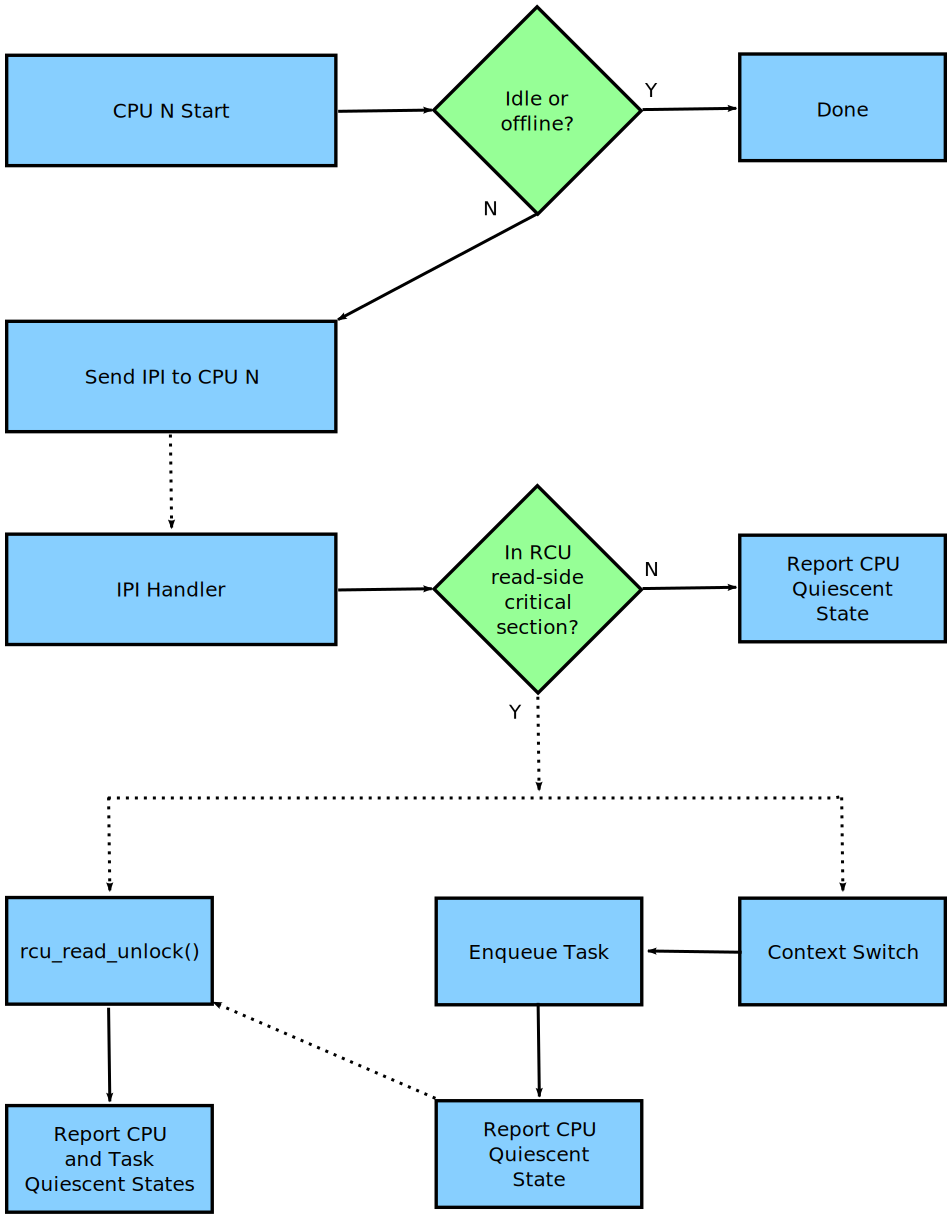
\includegraphics{rcu/design/ExpRCUFlow}}
\end{center}

The solid arrows denote direct action, for example, a function call.
The dotted arrows denote indirect action, for example, an IPI
or a state that is reached after some time.

If a given CPU is offline or idle, \co{synchronize_rcu_expedited()}
will ignore it because idle and offline CPUs are already residing
in quiescent states.
Otherwise, the expedited grace period will use
\co{smp_call_function_single()} to send the CPU an IPI, which
is handled by \co{rcu_exp_handler()}.

However, because this is preemptible RCU, \co{rcu_exp_handler()}
can check to see if the CPU is currently running in an RCU read-side
critical section.
If not, the handler can immediately report a quiescent state.
Otherwise, it sets flags so that the outermost \co{rcu_read_unlock()}
invocation will provide the needed quiescent-state report.
This flag-setting avoids the previous forced preemption of all
CPUs that might have RCU read-side critical sections.
In addition, this flag-setting is done so as to avoid increasing
the overhead of the common-case fastpath through the scheduler.

Again because this is preemptible RCU, an RCU read-side critical section
can be preempted.
When that happens, RCU will enqueue the task, which will the continue to
block the current expedited grace period until it resumes and finds its
outermost \co{rcu_read_unlock()}.
The CPU will report a quiescent state just after enqueuing the task because
the CPU is no longer blocking the grace period.
It is instead the preempted task doing the blocking.
The list of blocked tasks is managed by \co{rcu_preempt_ctxt_queue()},
which is called from \co{rcu_preempt_note_context_switch()}, which
in turn is called from \co{rcu_note_context_switch()}, which in
turn is called from the scheduler.


\QuickQuiz{
  Why not just have the expedited grace period check the state of all
  the CPUs?
  After all, that would avoid all those real-time-unfriendly
  IPIs.
}\QuickQuizAnswer{
  Because we want the RCU read-side critical sections to run fast,
  which means no memory barriers.
  Therefore, it is not possible to
  safely check the state from some other CPU\@.
  And even if it was
  possible to safely check the state, it would still be necessary to
  IPI the CPU to safely interact with the upcoming
  \co{rcu_read_unlock()} invocation, which means that the remote state
  testing would not help the worst-case latency that real-time
  applications care about.

  One way to prevent your real-time application from getting hit with
  these IPIs is to build your kernel with \co{CONFIG_NO_HZ_FULL=y}.
  RCU
  would then perceive the CPU running your application as being idle,
  and it would be able to safely detect that state without needing to
  IPI the CPU\@.
}\QuickQuizEnd

Please note that this is just the overall flow:
Additional complications
can arise due to races with CPUs going idle or offline, among other
things.

\subsection{RCU-sched Expedited Grace Periods}

\co{CONFIG_PREEMPTION=n} kernels implement RCU-sched.
The overall flow of
the handling of a given CPU by an RCU-sched expedited grace period is
shown in the following diagram:

\begin{center}
\resizebox{.6\columnwidth}{!}{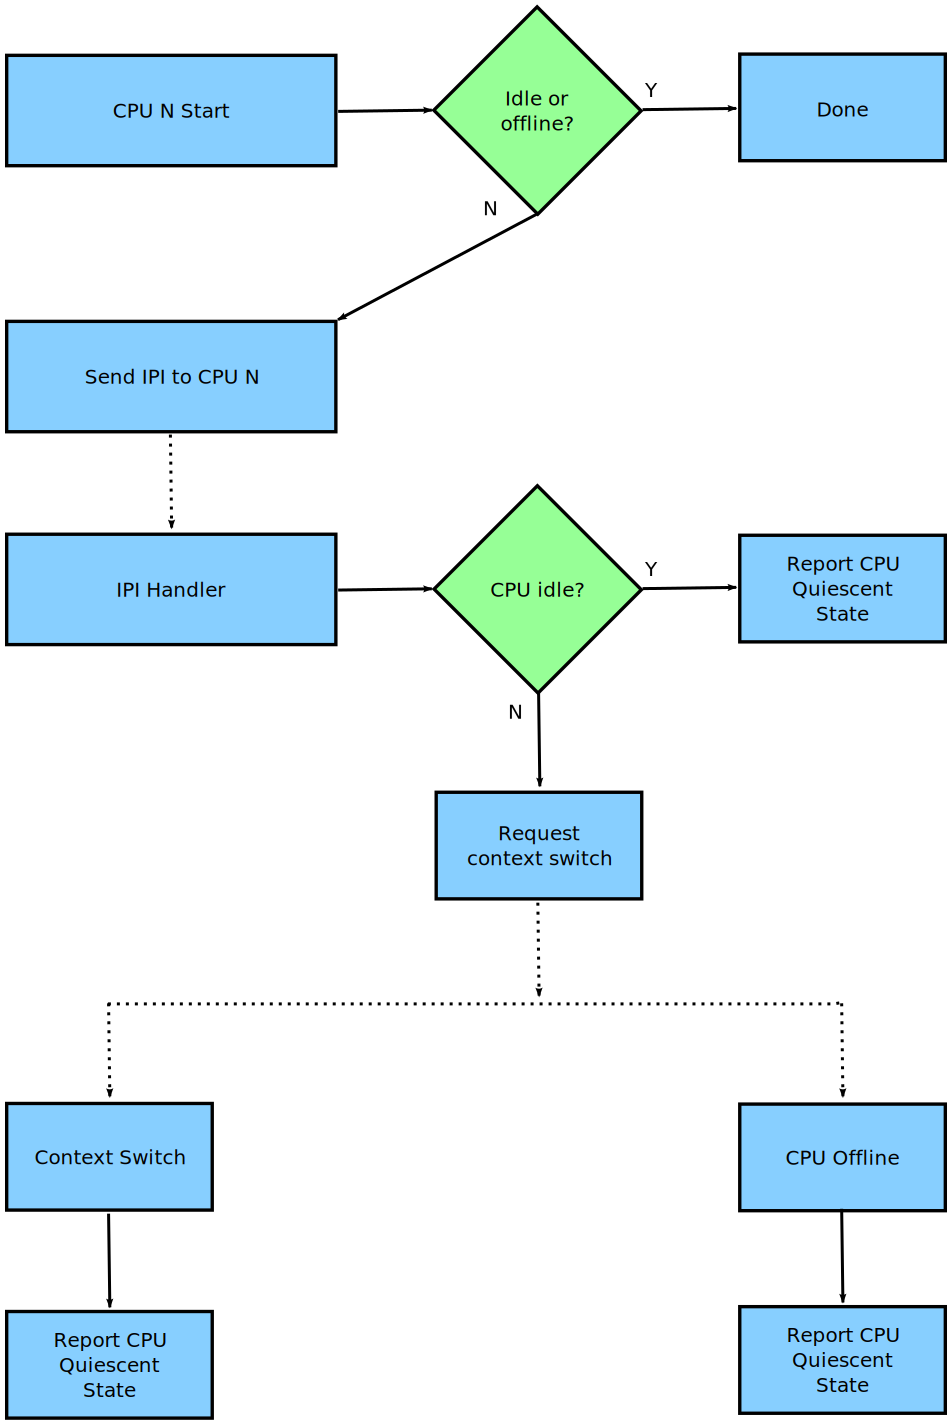
\includegraphics{rcu/design/ExpSchedFlow}}
\end{center}

As with RCU-preempt, RCU-sched's \co{synchronize_rcu_expedited()} ignores
offline and idle CPUs, again because they are in remotely detectable
quiescent states.
However, because the \co{rcu_read_lock_sched()} and
\co{rcu_read_unlock_sched()} leave no trace of their invocation, in
general it is not possible to tell whether or not the current CPU is in
an RCU read-side critical section.
The best that RCU-sched's
\co{rcu_exp_handler()} can do is to check for idle, on the off-chance
that the CPU went idle while the IPI was in flight.
If the CPU is idle,
then \co{rcu_exp_handler()} reports the quiescent state.

Otherwise, the handler forces a future context switch by setting the
\co{NEED_RESCHED} flag of the current task's thread flag and the CPU preempt
counter.
At the time of the context switch, the CPU reports the
quiescent state. Should the CPU go offline first, it will report the
quiescent state at that time.


\subsection{Expedited Grace Period and CPU Hotplug}

The expedited nature of expedited grace periods require a much tighter
interaction with CPU hotplug operations than is required for normal
grace periods.
In addition, attempting to IPI offline CPUs will result
in splats, but failing to IPI online CPUs can result in too-short grace
periods.
Neither option is acceptable in production kernels.

The interaction between expedited grace periods and CPU hotplug
operations is carried out at several levels:

\begin{enumerate}
\item The number of CPUs that have ever been online is tracked by the
   \co{rcu_state} structure's \co{->ncpus} field.
   The \co{rcu_state}
   structure's \co{->ncpus_snap} field tracks the number of CPUs that
   have ever been online at the beginning of an RCU expedited grace
   period.
   Note that this number never decreases, at least in the
   absence of a time machine.

\item The identities of the CPUs that have ever been online is tracked by
   the \co{rcu_node} structure's \co{->expmaskinitnext} field.
   The
   \co{rcu_node} structure's \co{->expmaskinit} field tracks the
   identities of the CPUs that were online at least once at the
   beginning of the most recent RCU expedited grace period.
   The
   \co{rcu_state} structure's \co{->ncpus} and \co{->ncpus_snap} fields are
   used to detect when new CPUs have come online for the first time,
   that is, when the \co{rcu_node} structure's \co{->expmaskinitnext}
   field has changed since the beginning of the last RCU expedited grace
   period, which triggers an update of each \co{rcu_node} structure's
   \co{->expmaskinit} field from its \co{->expmaskinitnext} field.

\item Each \co{rcu_node} structure's \co{->expmaskinit} field is used to
   initialize that structure's \co{->expmask} at the beginning of each
   RCU expedited grace period.
   This means that only those CPUs that have
   been online at least once will be considered for a given grace
   period.

\item Any CPU that goes offline will clear its bit in its leaf \co{rcu_node}
   structure's \co{->qsmaskinitnext} field, so any CPU with that bit
   clear can safely be ignored.
   However, it is possible for a CPU coming
   online or going offline to have this bit set for some time while
   \co{cpu_online} returns \co{false}.

\item For each non-idle CPU that RCU believes is currently online, the
   grace period invokes \co{smp_call_function_single()}.
   If this
   succeeds, the CPU was fully online.
   Failure indicates that the CPU is
   in the process of coming online or going offline, in which case it is
   necessary to wait for a short time period and try again.
   The purpose
   of this wait (or series of waits, as the case may be) is to permit a
   concurrent CPU-hotplug operation to complete.

\item In the case of RCU-sched, one of the last acts of an outgoing CPU is
   to invoke \co{rcutree_report_cpu_dead()}, which reports a quiescent state for
   that CPU\@.
   However, this is likely paranoia-induced redundancy.
\end{enumerate}

\QuickQuiz{
  Why all the dancing around with multiple counters and masks tracking
  CPUs that were once online? Why not just have a single set of masks
  tracking the currently online CPUs and be done with it?
}\QuickQuizAnswer{
  Maintaining single set of masks tracking the online CPUs \emph{sounds}
  easier, at least until you try working out all the race conditions
  between grace-period initialization and CPU-hotplug operations.
  For
  example, suppose initialization is progressing down the tree while a
  CPU-offline operation is progressing up the tree.
  This situation can
  result in bits set at the top of the tree that have no counterparts
  at the bottom of the tree.
  Those bits will never be cleared, which
  will result in grace-period hangs.
  In short, that way lies madness,
  to say nothing of a great many bugs, hangs, and deadlocks.
  In contrast, the current multi-mask multi-counter scheme ensures that
  grace-period initialization will always see consistent masks up and
  down the tree, which brings significant simplifications over the
  single-mask method.

  This is an instance of
  % dead link: http://www.cs.columbia.edu/~library/TR-repository/reports/reports-1992/cucs-039-92.ps.gz
  % Synthesis: an efficient implementation of fundamental operating system services
  % At ACM: https://dl.acm.org/doi/10.5555/143219
  \href{https://dl.acm.org/doi/10.5555/143219}
  {deferring work in order to avoid synchronization}.
  Lazily recording CPU-hotplug events at the beginning of the next
  grace period greatly simplifies maintenance of the CPU-tracking
  bitmasks in the \co{rcu_node} tree.
}\QuickQuizEnd


\subsection{Expedited Grace Period Refinements}

\subsubsection{Idle-CPU Checks}

Each expedited grace period checks for idle CPUs when initially forming
the mask of CPUs to be IPIed and again just before IPIing a CPU (both
checks are carried out by \co{sync_rcu_exp_select_cpus()}).
If the CPU is
idle at any time between those two times, the CPU will not be IPIed.
Instead, the task pushing the grace period forward will include the idle
CPUs in the mask passed to \co{rcu_report_exp_cpu_mult()}.

For RCU-sched, there is an additional check:
If the IPI has interrupted
the idle loop, then \co{rcu_exp_handler()} invokes
\co{rcu_report_exp_rdp()} to report the corresponding quiescent state.

For RCU-preempt, there is no specific check for idle in the IPI handler
(\co{rcu_exp_handler()}), but because RCU read-side critical sections are
not permitted within the idle loop, if \co{rcu_exp_handler()} sees that
the CPU is within RCU read-side critical section, the CPU cannot
possibly be idle.
Otherwise, \co{rcu_exp_handler()} invokes
\co{rcu_report_exp_rdp()} to report the corresponding quiescent state,
regardless of whether or not that quiescent state was due to the CPU
being idle.

In summary, RCU expedited grace periods check for idle when building the
bitmask of CPUs that must be IPIed, just before sending each IPI, and
(either explicitly or implicitly) within the IPI handler.

\subsubsection{Batching via Sequence Counter}

If each grace-period request was carried out separately, expedited grace
periods would have abysmal scalability and problematic high-load
characteristics.
Because each grace-period operation can serve an
unlimited number of updates, it is important to \emph{batch} requests, so
that a single expedited grace-period operation will cover all requests
in the corresponding batch.

This batching is controlled by a sequence counter named
\co{->expedited_sequence} in the \co{rcu_state} structure.
This counter
has an odd value when there is an expedited grace period in progress and
an even value otherwise, so that dividing the counter value by two gives
the number of completed grace periods.
During any given update request,
the counter must transition from even to odd and then back to even, thus
indicating that a grace period has elapsed.
Therefore, if the initial
value of the counter is \co{s}, the updater must wait until the counter
reaches at least the value \co{(s+3)&~0x1}.
This counter is managed by
the following access functions:

\begin{enumerate}
\item \co{rcu_exp_gp_seq_start()}, which marks the start of an expedited
   grace period.
\item \co{rcu_exp_gp_seq_end()}, which marks the end of an expedited grace
   period.
\item \co{rcu_exp_gp_seq_snap()}, which obtains a snapshot of the counter.
\item \co{rcu_exp_gp_seq_done()}, which returns \co{true} if a full expedited
   grace period has elapsed since the corresponding call to
   \co{rcu_exp_gp_seq_snap()}.
\end{enumerate}

Again, only one request in a given batch need actually carry out a
grace-period operation, which means there must be an efficient way to
identify which of many concurrent requests will initiate the grace
period, and that there be an efficient way for the remaining requests to
wait for that grace period to complete.
However, that is the topic of
the next section.

\subsubsection{Funnel Locking and Wait/Wakeup}

The natural way to sort out which of a batch of updaters will initiate
the expedited grace period is to use the \co{rcu_node} combining tree, as
implemented by the \co{exp_funnel_lock()} function.
The first updater
corresponding to a given grace period arriving at a given \co{rcu_node}
structure records its desired grace-period sequence number in the
\co{->exp_seq_rq} field and moves up to the next level in the tree.
Otherwise, if the \co{->exp_seq_rq} field already contains the sequence
number for the desired grace period or some later one, the updater
blocks on one of four wait queues in the \co{->exp_wq[]} array, using the
second-from-bottom and third-from bottom bits as an index.
An
\co{->exp_lock} field in the \co{rcu_node} structure synchronizes access
to these fields.

An empty \co{rcu_node} tree is shown in the following diagram, with the
white cells representing the \co{->exp_seq_rq} field and the red cells
representing the elements of the \co{->exp_wq[]} array.

\begin{center}
\resizebox{\columnwidth}{!}{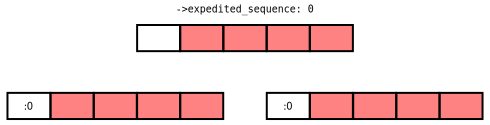
\includegraphics{rcu/design/Funnel0}}
\end{center}

The next diagram shows the situation after the arrival of Task~A and
Task~B at the leftmost and rightmost leaf \co{rcu_node} structures,
respectively.
The current value of the \co{rcu_state} structure's
\co{->expedited_sequence} field is zero, so adding three and clearing the
bottom bit results in the value two, which both tasks record in the
\co{->exp_seq_rq} field of their respective \co{rcu_node} structures:

\begin{center}
\resizebox{\columnwidth}{!}{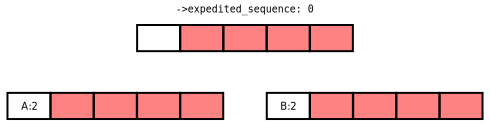
\includegraphics{rcu/design/Funnel1}}
\end{center}

Each of Tasks~A and~B will move up to the root \co{rcu_node} structure.
Suppose that Task~A wins, recording its desired grace-period sequence
number and resulting in the state shown below:

\begin{center}
\resizebox{\columnwidth}{!}{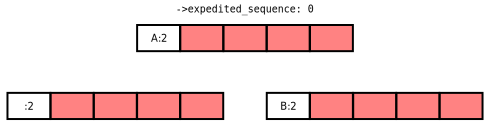
\includegraphics{rcu/design/Funnel2}}
\end{center}

Task~A now advances to initiate a new grace period, while Task~B moves
up to the root \co{rcu_node} structure, and, seeing that its desired
sequence number is already recorded, blocks on \co{->exp_wq[1]}.

\QuickQuiz{
  Why \co{->exp_wq[1]}?
  Given that the value of these tasks' desired
  sequence number is two, so shouldn't they instead block on
  \co{->exp_wq[2]}?
}\QuickQuizAnswer{
  No.
  Recall that the bottom bit of the desired sequence number indicates
  whether or not a grace period is currently in progress.
  It is
  therefore necessary to shift the sequence number right one bit
  position to obtain the number of the grace period.
  This results in
  \co{->exp_wq[1]}.
}\QuickQuizEnd

If Tasks~C and~D also arrive at this point, they will compute the same
desired grace-period sequence number, and see that both leaf
\co{rcu_node} structures already have that value recorded.
They will
therefore block on their respective \co{rcu_node} structures'
\co{->exp_wq[1]} fields, as shown below:

\begin{center}
\resizebox{\columnwidth}{!}{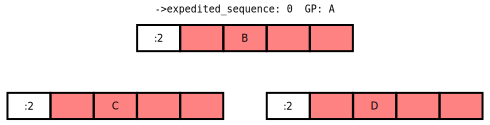
\includegraphics{rcu/design/Funnel3}}
\end{center}

Task~A now acquires the \co{rcu_state} structure's \co{->exp_mutex} and
initiates the grace period, which increments \co{->expedited_sequence}.
Therefore, if Tasks~E and~F arrive, they will compute a desired sequence
number of 4 and will record this value as shown below:

\begin{center}
\resizebox{\columnwidth}{!}{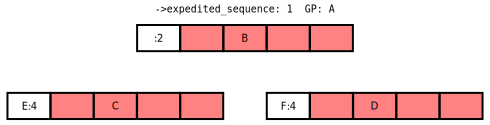
\includegraphics{rcu/design/Funnel4}}
\end{center}

Tasks~E and~F will propagate up the \co{rcu_node} combining tree, with
Task~F blocking on the root \co{rcu_node} structure and Task~E wait for
Task~A to finish so that it can start the next grace period.
The
resulting state is as shown below:

\begin{center}
\resizebox{\columnwidth}{!}{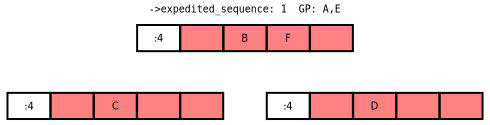
\includegraphics{rcu/design/Funnel5}}
\end{center}

Once the grace period completes, Task~A starts waking up the tasks
waiting for this grace period to complete, increments the
\co{->expedited_sequence}, acquires the \co{->exp_wake_mutex} and then
releases the \co{->exp_mutex}.
This results in the following state:

\begin{center}
\resizebox{\columnwidth}{!}{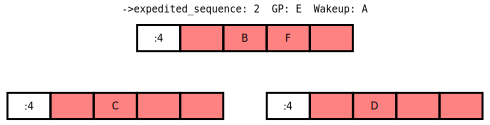
\includegraphics{rcu/design/Funnel6}}
\end{center}

Task~E can then acquire \co{->exp_mutex} and increment
\co{->expedited_sequence} to the value three.
If new tasks~G and~H arrive
and moves up the combining tree at the same time, the state will be as
follows:

\begin{center}
\resizebox{\columnwidth}{!}{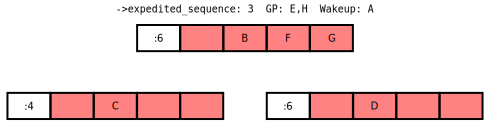
\includegraphics{rcu/design/Funnel7}}
\end{center}

Note that three of the root \co{rcu_node} structure's waitqueues are now
occupied.
However, at some point, Task~A will wake up the tasks blocked
on the \co{->exp_wq} waitqueues, resulting in the following state:

\begin{center}
\resizebox{\columnwidth}{!}{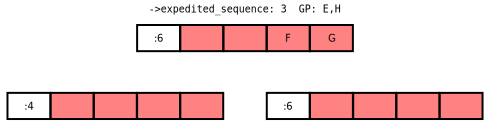
\includegraphics{rcu/design/Funnel8}}
\end{center}

Execution will continue with Tasks~E and~H completing their grace
periods and carrying out their wakeups.

\QuickQuiz{
  What happens if Task~A takes so long to do its wakeups that Task~E's
  grace period completes?
}\QuickQuizAnswer{
  Then Task~E will block on the \co{->exp_wake_mutex}, which will also
  prevent it from releasing \co{->exp_mutex}, which in turn will prevent
  the next grace period from starting.
  This last is important in
  preventing overflow of the \co{->exp_wq[]} array.
}\QuickQuizEnd

\subsubsection{Use of Workqueues}

In earlier implementations, the task requesting the expedited grace
period also drove it to completion.
This straightforward approach had
the disadvantage of needing to account for POSIX signals sent to user
tasks, so more recent implementations use the Linux kernel's
workqueues (see \path{Documentation/core-api/workqueue.rst}).

The requesting task still does counter snapshotting and funnel-lock
processing, but the task reaching the top of the funnel lock does a
\co{schedule_work()} (from \co{_synchronize_rcu_expedited()} so that a
workqueue kthread does the actual grace-period processing.
Because
workqueue kthreads do not accept POSIX signals, grace-period-wait
processing need not allow for POSIX signals.
In addition, this approach
allows wakeups for the previous expedited grace period to be overlapped
with processing for the next expedited grace period.
Because there are
only four sets of waitqueues, it is necessary to ensure that the
previous grace period's wakeups complete before the next grace period's
wakeups start.
This is handled by having the \co{->exp_mutex} guard
expedited grace-period processing and the \co{->exp_wake_mutex} guard
wakeups.
The key point is that the \co{->exp_mutex} is not released until
the first wakeup is complete, which means that the \co{->exp_wake_mutex}
has already been acquired at that point.
This approach ensures that the
previous grace period's wakeups can be carried out while the current
grace period is in process, but that these wakeups will complete before
the next grace period starts.
This means that only three waitqueues are
required, guaranteeing that the four that are provided are sufficient.

\subsubsection{Stall Warnings}

Expediting grace periods does nothing to speed things up when RCU
readers take too long, and therefore expedited grace periods check for
stalls just as normal grace periods do.

\QuickQuiz{
  But why not just let the normal grace-period machinery detect the
  stalls, given that a given reader must block both normal and
  expedited grace periods?
}\QuickQuizAnswer{
  Because it is quite possible that at a given time there is no normal
  grace period in progress, in which case the normal grace period
  cannot emit a stall warning.
}\QuickQuizEnd

The \co{synchronize_sched_expedited_wait()} function loops waiting for
the expedited grace period to end, but with a timeout set to the current
RCU CPU stall-warning time.
If this time is exceeded, any CPUs or
\co{rcu_node} structures blocking the current grace period are printed.
Each stall warning results in another pass through the loop, but the
second and subsequent passes use longer stall times.

\subsubsection{Mid-boot operation}

The use of workqueues has the advantage that the expedited grace-period
code need not worry about POSIX signals.
Unfortunately, it has the
corresponding disadvantage that workqueues cannot be used until they are
initialized, which does not happen until some time after the scheduler
spawns the first task.
Given that there are parts of the kernel that
really do want to execute grace periods during this mid-boot ``dead
zone'', expedited grace periods must do something else during this time.

What they do is to fall back to the old practice of requiring that the
requesting task drive the expedited grace period, as was the case before
the use of workqueues.
However, the requesting task is only required to
drive the grace period during the mid-boot dead zone.
Before mid-boot, a
synchronous grace period is a no-op. Some time after mid-boot,
workqueues are used.

Non-expedited non-SRCU synchronous grace periods must also operate
normally during mid-boot.
This is handled by causing non-expedited grace
periods to take the expedited code path during mid-boot.

The current code assumes that there are no POSIX signals during the
mid-boot dead zone.
However, if an overwhelming need for POSIX signals
somehow arises, appropriate adjustments can be made to the expedited
stall-warning code.
One such adjustment would reinstate the
pre-workqueue stall-warning checks, but only during the mid-boot dead
zone.

With this refinement, synchronous grace periods can now be used from
task context pretty much any time during the life of the kernel.
That
is, aside from some points in the suspend, hibernate, or shutdown code
path.

\subsection{Summary}

Expedited grace periods use a sequence-number approach to promote
batching, so that a single grace-period operation can serve numerous
requests.
A funnel lock is used to efficiently identify the one task out
of a concurrent group that will request the grace period.
All members of
the group will block on waitqueues provided in the \co{rcu_node}
structure.
The actual grace-period processing is carried out by a
workqueue.

CPU-hotplug operations are noted lazily in order to prevent the need for
tight synchronization between expedited grace periods and CPU-hotplug
operations.
The dyntick-idle counters are used to avoid sending IPIs to
idle CPUs, at least in the common case. RCU-preempt and RCU-sched use
different IPI handlers and different code to respond to the state
changes carried out by those handlers, but otherwise use common code.

Quiescent states are tracked using the \co{rcu_node} tree, and once all
necessary quiescent states have been reported, all tasks waiting on this
expedited grace period are awakened.
A pair of mutexes are used to allow
one grace period's wakeups to proceed concurrently with the next grace
period's processing.

This combination of mechanisms allows expedited grace periods to run
reasonably efficiently.
However, for non-time-critical tasks, normal
grace periods should be used instead because their longer duration
permits much higher degrees of batching, and thus much lower per-request
overheads.

%\section{A Tour Through RCU's Requirements}
\label{sec:rcu:A Tour Through RCU's Requirements}

\begin{Note}
Copyright IBM Corporation, 2015

Author: Paul E. McKenney

The initial version of this document appeared in the
\href{https://lwn.net/}{LWN} on those articles:
\href{https://lwn.net/Articles/652156/}{part 1},
\href{https://lwn.net/Articles/652677/}{part 2}, and
\href{https://lwn.net/Articles/653326/}{part 3}.
\end{Note}


\subsection{Introduction}

Read-copy update (RCU) is a synchronization mechanism that is often used
as a replacement for reader-writer locking.
RCU is unusual in that
updaters do not block readers, which means that RCU's read-side
primitives can be exceedingly fast and scalable.
In addition, updaters
can make useful forward progress concurrently with readers.
However, all
this concurrency between RCU readers and updaters does raise the
question of exactly what RCU readers are doing, which in turn raises the
question of exactly what RCU's requirements are.

This document therefore summarizes RCU's requirements, and can be
thought of as an informal, high-level specification for RCU\@.
It is
important to understand that RCU's specification is primarily empirical
in nature; in fact, I learned about many of these requirements the hard
way.
This situation might cause some consternation, however, not only
has this learning process been a lot of fun, but it has also been a
great privilege to work with so many people willing to apply
technologies in interesting new ways.

All that aside, here are the categories of currently known RCU
requirements:

\begin{enumerate}
\item Fundamental Requirements
\item Fundamental Non-Requirements
\item Parallelism Facts of Life
\item Quality-of-Implementation Requirements
\item Linux Kernel Complications
\item Software-Engineering Requirements
\item Other RCU Flavors
\item Possible Future Changes
\end{enumerate}

This is followed by a summary.

%however, the answers to
%each quick quiz immediately follows the quiz.
%Select the big white space
%with your mouse to see the answer.

\begin{Note}
  Quick Quizzes are rendered by perfbook's scheme, where the answers
  go to a later chapter.
  Each pair of quiz and answer is cross-referenced by hyper-links in
  the PDF\@.
\end{Note}

\subsection{Fundamental Requirements}

RCU's fundamental requirements are the closest thing RCU has to hard
mathematical requirements.
These are:

\begin{enumerate}
\item Grace-Period Guarantee
\item Publish/Subscribe Guarantee
\item Memory-Barrier Guarantees
\item RCU Primitives Guaranteed to Execute Unconditionally
\item Guaranteed Read-to-Write Upgrade
\end{enumerate}

\subsubsection{Grace-Period Guarantee}

RCU's grace-period guarantee is unusual in being premeditated:
Jack
Slingwine and I had this guarantee firmly in mind when we started work
on RCU (then called “rclock”) in the early 1990s.
That said, the past
two decades of experience with RCU have produced a much more detailed
understanding of this guarantee.

RCU's grace-period guarantee allows updaters to wait for the completion
of all pre-existing RCU read-side critical sections.
An RCU read-side
critical section begins with the marker \co{rcu_read_lock()} and ends
with the marker \co{rcu_read_unlock()}.
These markers may be nested, and
RCU treats a nested set as one big RCU read-side critical section.
Production-quality implementations of \co{rcu_read_lock()} and
\co{rcu_read_unlock()} are extremely lightweight, and in fact have
exactly zero overhead in Linux kernels built for production use with
\co{CONFIG_PREEMPTION=n}.

This guarantee allows ordering to be enforced with extremely low
overhead to readers, for example:

\begin{fcvlabel}[ln:rcu:desing:req1]
\begin{VerbatimN}[commandchars=\%\@\$]
	int x, y;

	void thread0(void)
	{
		rcu_read_lock();
		r1 = READ_ONCE(x);
		r2 = READ_ONCE(y);
		rcu_read_unlock();
	}

	void thread1(void)
	{
		WRITE_ONCE(x, 1);
		synchronize_rcu(); %lnlbl@sync$
		WRITE_ONCE(y, 1);
	}
\end{VerbatimN}
\end{fcvlabel}

\begin{fcvref}[ln:rcu:desing:req1]
Because the \co{synchronize_rcu()} on \clnref{sync} % line 14
waits for all pre-existing
readers, any instance of \co{thread0()} that loads a value of zero
from~\co{x} must complete before \co{thread1()} stores to~\co{y}, so that
instance must also load a value of zero from~\co{y}.
Similarly, any
instance of \co{thread0()} that loads a value of one from~\co{y} must have
started after the \co{synchronize_rcu()} started, and must therefore also
load a value of one from~\co{x}.
\end{fcvref}
Therefore, the outcome:

\begin{VerbatimU}
	(r1 == 0 && r2 == 1)
\end{VerbatimU}

\noindent%
cannot happen.

\QuickQuiz{
  Wait a minute!
  You said that updaters can make useful forward
  progress concurrently with readers, but pre-existing readers will
  block \co{synchronize_rcu()}!!!
  Just who are you trying to fool???
}\QuickQuizAnswer{
  First, if updaters do not wish to be blocked by readers, they can use
  \co{call_rcu()} or \co{kfree_rcu()}, which will be discussed later.
  Second, even when using \co{synchronize_rcu()}, the other update-side
  code does run concurrently with readers, whether pre-existing or not.
}\QuickQuizEnd

This scenario resembles one of the first uses of RCU in
\href{https://en.wikipedia.org/wiki/DYNIX}{DYNIX/ptx}, which managed a
distributed lock manager's transition into a state suitable for handling
recovery from node failure, more or less as follows:

\begin{fcvlabel}[ln:rcu:design:req2]
\begin{VerbatimN}[commandchars=\%\@\$]
	#define STATE_NORMAL        0
	#define STATE_WANT_RECOVERY 1
	#define STATE_RECOVERING    2
	#define STATE_WANT_NORMAL   3

	int state = STATE_NORMAL;

	void do_something_dlm(void)
	{
		int state_snap;

		rcu_read_lock();
		state_snap = READ_ONCE(state);
		if (state_snap == STATE_NORMAL)
			do_something();
		else
			do_something_carefully();
		rcu_read_unlock();
	}

	void start_recovery(void)
	{
		WRITE_ONCE(state, STATE_WANT_RECOVERY);
		synchronize_rcu();
		WRITE_ONCE(state, STATE_RECOVERING);
		recovery();
		WRITE_ONCE(state, STATE_WANT_NORMAL);
		synchronize_rcu();   %lnlbl@sync2$
		WRITE_ONCE(state, STATE_NORMAL);
	}
\end{VerbatimN}
\end{fcvlabel}

The RCU read-side critical section in \co{do_something_dlm()} works with
the \co{synchronize_rcu()} in \co{start_recovery()} to guarantee that
\co{do_something()} never runs concurrently with \co{recovery()}, but with
little or no synchronization overhead in \co{do_something_dlm()}.

\QuickQuiz{
\begin{fcvref}[ln:rcu:design:req2]
  Why is the \co{synchronize_rcu()} on \clnref{sync2} %line 28
  needed?
\end{fcvref}
}\QuickQuizAnswer{
  Without that extra grace period, memory reordering could result in
  \co{do_something_dlm()} executing \co{do_something()} concurrently with
  the last bits of \co{recovery(}.
}\QuickQuizEnd

In order to avoid fatal problems such as deadlocks, an RCU read-side
critical section must not contain calls to \co{synchronize_rcu()}.
Similarly, an RCU read-side critical section must not contain anything
that waits, directly or indirectly, on completion of an invocation of
\co{synchronize_rcu()}.

Although RCU's grace-period guarantee is useful in and of itself, with
\href{https://lwn.net/Articles/573497/}{quite a few use cases}, it would
be good to be able to use RCU to coordinate read-side access to linked
data structures.
For this, the grace-period guarantee is not sufficient,
as can be seen in function \co{add_gp_buggy()} below.
We will look at the
reader's code later, but in the meantime, just think of the reader as
locklessly picking up the \co{gp} pointer, and, if the value loaded is
non-\co{NULL}, locklessly accessing the \co{->a} and \co{->b} fields.

\begin{VerbatimN}
	bool add_gp_buggy(int a, int b)
	{
		p = kmalloc(sizeof(*p), GFP_KERNEL);
		if (!p)
			return -ENOMEM;
		spin_lock(&gp_lock);
                if (rcu_access_pointer(gp)) {
			spin_unlock(&gp_lock);
			return false;
		}
		p->a = a;
		p->b = a;
		gp = p; /* ORDERING BUG */
		spin_unlock(&gp_lock);
		return true;
	}
\end{VerbatimN}

The problem is that both the compiler and weakly ordered CPUs are within
their rights to reorder this code as follows:

\begin{fcvlabel}[ln:rcu:design:req3]
\begin{VerbatimN}[commandchars=\%\@\$]
	bool add_gp_buggy_optimized(int a, int b)
	{
		p = kmalloc(sizeof(*p), GFP_KERNEL);
		if (!p)
			return -ENOMEM;
		spin_lock(&gp_lock);
		if (rcu_access_pointer(gp)) {
			spin_unlock(&gp_lock);
			return false;
		}
		gp = p; /* ORDERING BUG */ %lnlbl@bug$
		p->a = a;
		p->b = a;
		spin_unlock(&gp_lock);
		return true;
	}
\end{VerbatimN}
\end{fcvlabel}

\begin{fcvref}[ln:rcu:design:req3]
If an RCU reader fetches \co{gp} just after \co{add_gp_buggy_optimized}
executes \clnref{bug}, % line 11
it will see garbage in the \co{->a} and \co{->b} fields.
\end{fcvref}
And this is but one of many ways in which compiler and hardware
optimizations could cause trouble.
Therefore, we clearly need some way
to prevent the compiler and the CPU from reordering in this manner,
which brings us to the publish-subscribe guarantee discussed in the next
section.

\subsubsection{Publish/Subscribe Guarantee}

RCU's publish-subscribe guarantee allows data to be inserted into a
linked data structure without disrupting RCU readers.
The updater uses
\co{rcu_assign_pointer()} to insert the new data, and readers use
\co{rcu_dereference()} to access data, whether new or old.
The following
shows an example of insertion:

\begin{fcvlabel}[ln:rcu:design:rcu4]
\begin{VerbatimN}[commandchars=\%\@\$]
	bool add_gp(int a, int b)
	{
		p = kmalloc(sizeof(*p), GFP_KERNEL);
		if (!p)
			return -ENOMEM;
		spin_lock(&gp_lock);
		if (rcu_access_pointer(gp)) {
			spin_unlock(&gp_lock);
			return false;
		}
		p->a = a;                   %lnlbl@a$
		p->b = a;                   %lnlbl@b$
		rcu_assign_pointer(gp, p);  %lnlbl@assign$
		spin_unlock(&gp_lock);
		return true;
	}
\end{VerbatimN}
\end{fcvlabel}

\begin{fcvref}[ln:rcu:design:rcu4]
The \co{rcu_assign_pointer()} on \clnref{assign} % line 13
is conceptually equivalent to a
simple assignment statement, but also guarantees that its assignment
will happen after the two assignments in \clnref{a,b}, %lines 11 and 12
similar to the
C11 \co{memory_order_release} store operation.
\end{fcvref}
It also prevents any
number of ``interesting'' compiler optimizations, for example, the use of
\co{gp} as a scratch location immediately preceding the assignment.

\QuickQuiz{
  But \co{rcu_assign_pointer()} does nothing to prevent the two
  assignments to \co{p->a} and \co{p->b} from being reordered.
  Can't that
  also cause problems?
}\QuickQuizAnswer{
  No, it cannot. The readers cannot see either of these two fields
  until the assignment to \co{gp}, by which time both fields are fully
  initialized.
  So reordering the assignments to \co{p->a} and \co{p->b}
  cannot possibly cause any problems.
}\QuickQuizEnd

It is tempting to assume that the reader need not do anything special to
control its accesses to the RCU-protected data, as shown in
\co{do_something_gp_buggy()} below:

\begin{VerbatimN}
	bool do_something_gp_buggy(void)
	{
		rcu_read_lock();
		p = gp;  /* OPTIMIZATIONS GALORE!!! */
		if (p) {
			do_something(p->a, p->b);
			rcu_read_unlock();
			return true;
		}
		rcu_read_unlock();
		return false;
	}
\end{VerbatimN}

However, this temptation must be resisted because there are a
surprisingly large number of ways that the compiler (or weak ordering
CPUs like the DEC Alpha) can trip this code up.
For but one example, if
the compiler were short of registers, it might choose to refetch from
\co{gp} rather than keeping a separate copy in~\co{p} as follows:

\begin{VerbatimN}
	bool do_something_gp_buggy_optimized(void)
	{
		rcu_read_lock();
		if (gp) { /* OPTIMIZATIONS GALORE!!! */
			do_something(gp->a, gp->b);
			rcu_read_unlock();
			return true;
		}
		rcu_read_unlock();
		return false;
	}
\end{VerbatimN}

If this function ran concurrently with a series of updates that replaced
the current structure with a new one, the fetches of \co{gp->a}n and
\co{gp->b} might well come from two different structures, which could
cause serious confusion.
To prevent this (and much else besides),
\co{do_something_gp()} uses \co{rcu_dereference()} to fetch from \co{gp}:

\begin{fcvlabel}[ln:rcu:design:req5]
\begin{VerbatimN}[commandchars=\%\@\$]
	bool do_something_gp(void)
	{
		rcu_read_lock();
		p = rcu_dereference(gp);
		if (p) {
			do_something(p->a, p->b);
			rcu_read_unlock();    %lnlbl@unlock$
			return true;
		}
		rcu_read_unlock();
		return false;
	}
\end{VerbatimN}
\end{fcvlabel}

The \co{rcu_dereference()} uses volatile casts and (for DEC Alpha) memory
barriers in the Linux kernel.
Should a
\href{http://www.rdrop.com/users/paulmck/RCU/consume.2015.07.13a.pdf}
{high-quality implementation of C11 \co{memory_order_consume} [PDF]}
ever appear, then \co{rcu_dereference()} could be implemented as a
\co{memory_order_consume} load. Regardless of the exact implementation, a
pointer fetched by \co{rcu_dereference()} may not be used outside of the
outermost RCU read-side critical section containing that
\co{rcu_dereference()}, unless protection of the corresponding data
element has been passed from RCU to some other synchronization
mechanism, most commonly locking or reference counting
(see \path{../../rcuref.rst}).

In short, updaters use \co{rcu_assign_pointer()} and readers use
\co{rcu_dereference()}, and these two RCU API elements work together to
ensure that readers have a consistent view of newly added data elements.

Of course, it is also necessary to remove elements from RCU-protected
data structures, for example, using the following process:

\begin{enumerate}
\item Remove the data element from the enclosing structure.
\item Wait for all pre-existing RCU read-side critical sections to complete
   (because only pre-existing readers can possibly have a reference to
   the newly removed data element).
\item At this point, only the updater has a reference to the newly removed
   data element, so it can safely reclaim the data element, for example,
   by passing it to \co{kfree()}.
\end{enumerate}

This process is implemented by \co{remove_gp_synchronous()}:

\begin{fcvlabel}[ln:rcu:design:req6]
\begin{VerbatimN}[commandchars=\%\@\$]
	bool remove_gp_synchronous(void)
	{
		struct foo *p;

		spin_lock(&gp_lock);
		p = rcu_access_pointer(gp);  %lnlbl@access$
		if (!p) {
			spin_unlock(&gp_lock);
			return false;
		}
		rcu_assign_pointer(gp, NULL);  %lnlbl@null$
		spin_unlock(&gp_lock);
		synchronize_rcu();    %lnlbl@sync$
		kfree(p);             %lnlbl@kfree$
		return true;
	}
\end{VerbatimN}
\end{fcvlabel}

\begin{fcvref}[ln:rcu:design:req6]
This function is straightforward, with \clnref{sync} % line13
waiting for a grace
period before \clnref{kfree} % line 14
frees the old data element.
\end{fcvref}
\begin{fcvref}[ln:rcu:design:req5]
This waiting ensures
that readers will reach \clnref{unlock} % line 7
of \co{do_something_gp()} before the data
element referenced by~\co{p} is freed.
\end{fcvref}
\begin{fcvref}[ln:rcu:design:req6]
The \co{rcu_access_pointer()} on \clnref{access} % line 6
is similar to \co{rcu_dereference()}, except that:
\end{fcvref}

\begin{enumerate}
\item The value returned by \co{rcu_access_pointer()} cannot be
   dereferenced. If you want to access the value pointed to as well as
   the pointer itself, use \co{rcu_dereference()} instead of
   \co{rcu_access_pointer()}.
\item The call to \co{rcu_access_pointer()} need not be protected.
   In
   contrast, \co{rcu_dereference()} must either be within an RCU
   read-side critical section or in a code segment where the pointer
   cannot change, for example, in code protected by the corresponding
   update-side lock.
\end{enumerate}

\QuickQuiz{
  Without the \co{rcu_dereference()} or the \co{rcu_access_pointer()},
  what destructive optimizations might the compiler make use of?
}\QuickQuizAnswer{
  Let's start with what happens to \co{do_something_gp()} if it fails to
  use \co{rcu_dereference()}.
  It could reuse a value formerly fetched
  from this same pointer.
  It could also fetch the pointer from \co{gp}
  in a byte-at-a-time manner, resulting in \emph{load tearing}, in turn
  resulting a bytewise mash-up of two distinct pointer values.
  It might
  even use value-speculation optimizations, where it makes a wrong
  guess, but by the time it gets around to checking the value, an
  update has changed the pointer to match the wrong guess.
  Too bad
  about any dereferences that returned pre-initialization garbage in
  the meantime!
  For \co{remove_gp_synchronous()}, as long as all modifications to
  \co{gp} are carried out while holding \co{gp_lock}, the above
  optimizations are harmless.
  However, \co{sparse} will complain if you
  define \co{gp} with \co{__rcu} and then access it without using either
  \co{rcu_access_pointer()} or \co{rcu_dereference()}.
}\QuickQuizEnd

In short, RCU's publish-subscribe guarantee is provided by the
combination of \co{rcu_assign_pointer()} and \co{rcu_dereference()}.
This
guarantee allows data elements to be safely added to RCU-protected
linked data structures without disrupting RCU readers.
This guarantee
can be used in combination with the grace-period guarantee to also allow
data elements to be removed from RCU-protected linked data structures,
again without disrupting RCU readers.

This guarantee was only partially premeditated.
DYNIX/ptx used an
explicit memory barrier for publication, but had nothing resembling
\co{rcu_dereference()} for subscription, nor did it have anything
resembling the dependency-ordering barrier that was later subsumed
into \co{rcu_dereference()} and later still into \co{READ_ONCE()}.
The
need for these operations made itself known quite suddenly at a
late-1990s meeting with the DEC Alpha architects, back in the days when
DEC was still a free-standing company.
It took the Alpha architects a
good hour to convince me that any sort of barrier would ever be needed,
and it then took me a good \emph{two} hours to convince them that their
documentation did not make this point clear.
More recent work with the C
and C++ standards committees have provided much education on tricks and
traps from the compiler.
In short, compilers were much less tricky in
the early 1990s, but in 2015, don't even think about omitting
\co{rcu_dereference()}!


\subsubsection{Memory-Barrier Guarantees}

The previous section's simple linked-data-structure scenario clearly
demonstrates the need for RCU's stringent memory-ordering guarantees on
systems with more than one CPU\@:

\begin{fcvref}[ln:rcu:design:req6]
\begin{enumerate}
\item Each CPU that has an RCU read-side critical section that begins
   before \co{synchronize_rcu()} starts is guaranteed to execute a full
   memory barrier between the time that the RCU read-side critical
   section ends and the time that \co{synchronize_rcu()} returns.
   Without
   this guarantee, a pre-existing RCU read-side critical section might
   hold a reference to the newly removed \co{struct foo} after the
   \co{kfree()} on \clnref{kfree} % line 14
   of \co{remove_gp_synchronous()}.
\item Each CPU that has an RCU read-side critical section that ends after
   \co{synchronize_rcu()} returns is guaranteed to execute a full memory
   barrier between the time that \co{synchronize_rcu()} begins and the
   time that the RCU read-side critical section begins.
   Without this
   guarantee, a later RCU read-side critical section running after the
   \co{kfree()} on \clnref{kfree} % line 14
   of \co{remove_gp_synchronous()} might later run
   \co{do_something_gp()} and find the newly deleted \co{struct foo}.
\item If the task invoking \co{synchronize_rcu()} remains on a given CPU,
   then that CPU is guaranteed to execute a full memory barrier sometime
   during the execution of \co{synchronize_rcu()}.
   This guarantee ensures
   that the \co{kfree()} on \clnref{kfree} % line 14
   of \co{remove_gp_synchronous()} really
   does execute after the removal on \clnref{null}. % line 11
\item If the task invoking \co{synchronize_rcu()} migrates among a group of
   CPUs during that invocation, then each of the CPUs in that group is
   guaranteed to execute a full memory barrier sometime during the
   execution of \co{synchronize_rcu()}.
   This guarantee also ensures that
   the \co{kfree()} on \clnref{kfree} % line 14
   of \co{remove_gp_synchronous()} really does
   execute after the removal on \clnref{null}, % line 11
   but also in the case where the
   thread executing the \co{synchronize_rcu()} migrates in the meantime.
\end{enumerate}
\end{fcvref}

\QuickQuiz{
  Given that multiple CPUs can start RCU read-side critical sections at
  any time without any ordering whatsoever, how can RCU possibly tell
  whether or not a given RCU read-side critical section starts before a
  given instance of \co{synchronize_rcu()}?
}\QuickQuizAnswer{
  If RCU cannot tell whether or not a given RCU read-side critical
  section starts before a given instance of \co{synchronize_rcu()}, then
  it must assume that the RCU read-side critical section started first.
  In other words, a given instance of \co{synchronize_rcu()} can avoid
  waiting on a given RCU read-side critical section only if it can
  prove that \co{synchronize_rcu()} started first.
  A related question is ``When \co{rcu_read_lock()} doesn't generate any
  code, why does it matter how it relates to a grace period?''
  The
  answer is that it is not the relationship of \co{rcu_read_lock()}
  itself that is important, but rather the relationship of the code
  within the enclosed RCU read-side critical section to the code
  preceding and following the grace period.
  If we take this viewpoint,
  then a given RCU read-side critical section begins before a given
  grace period when some access preceding the grace period observes the
  effect of some access within the critical section, in which case none
  of the accesses within the critical section may observe the effects
  of any access following the grace period.

  As of late 2016, mathematical models of RCU take this viewpoint, for
  example, see slides 62 and 63 of the
  \href{http://www2.rdrop.com/users/paulmck/scalability/paper/LinuxMM.2016.10.04c.LCE.pdf}{2016 LinuxCon}
  presentation.
}\QuickQuizEnd

\QuickQuiz{
  The first and second guarantees require unbelievably strict ordering!
  Are all these memory barriers \emph{really} required?
}\QuickQuizAnswer{
  Yes, they really are required.
  To see why the first guarantee is
  required, consider the following sequence of events:

  \begin{enumerate}
  \item CPU 1: \co{rcu_read_lock()}
  \item CPU 1: \co{q = rcu_dereference(gp); /* Very likely to return p. */}
  \item CPU 0: \co{list_del_rcu(p);}
  \item CPU 0: \co{synchronize_rcu()} starts.
  \item CPU 1: \co{do_something_with(q->a);} \\
     \co{/* No smp_mb(), so might happen after kfree(). */}
  \item CPU 1: \co{rcu_read_unlock()}
  \item CPU 0: \co{synchronize_rcu()} returns.
  \item CPU 0: \co{kfree(p);}
  \end{enumerate}

  Therefore, there absolutely must be a full memory barrier between the
  end of the RCU read-side critical section and the end of the grace
  period.

  The sequence of events demonstrating the necessity of the second rule
  is roughly similar:

  \begin{enumerate}
  \item CPU 0: \co{list_del_rcu(p);}
  \item CPU 0: \co{synchronize_rcu()} starts.
  \item CPU 1: \co{rcu_read_lock()}
  \item CPU 1: \co{q = rcu_dereference(gp);} \\
     \co{/* Might return p if no memory barrier. */}
  \item CPU 0: \co{synchronize_rcu()} returns.
  \item CPU 0: \co{kfree(p);}
  \item CPU 1: \co{do_something_with(q->a); /* Boom!!! */}
  \item CPU 1: \co{rcu_read_unlock()}
  \end{enumerate}

  And similarly, without a memory barrier between the beginning of the
  grace period and the beginning of the RCU read-side critical section,
  CPU~1 might end up accessing the freelist.

  The ``as if'' rule of course applies, so that any implementation that
  acts as if the appropriate memory barriers were in place is a correct
  implementation.
  That said, it is much easier to fool yourself into
  believing that you have adhered to the as-if rule than it is to
  actually adhere to it!
}\QuickQuizEnd

\QuickQuiz{
  You claim that \co{rcu_read_lock()} and \co{rcu_read_unlock()} generate
  absolutely no code in some kernel builds.
  This means that the
  compiler might arbitrarily rearrange consecutive RCU read-side
  critical sections.
  Given such rearrangement, if a given RCU read-side
  critical section is done, how can you be sure that all prior RCU
  read-side critical sections are done? Won't the compiler
  rearrangements make that impossible to determine?
}\QuickQuizAnswer{
  In cases where \co{rcu_read_lock()} and \co{rcu_read_unlock()} generate
  absolutely no code, RCU infers quiescent states only at special
  locations, for example, within the scheduler.
  Because calls to
  \co{schedule()} had better prevent calling-code accesses to shared
  variables from being rearranged across the call to \co{schedule()}, if
  RCU detects the end of a given RCU read-side critical section, it
  will necessarily detect the end of all prior RCU read-side critical
  sections, no matter how aggressively the compiler scrambles the code.
  Again, this all assumes that the compiler cannot scramble code across
  calls to the scheduler, out of interrupt handlers, into the idle
  loop, into user-mode code, and so on. But if your kernel build allows
  that sort of scrambling, you have broken far more than just RCU!
}\QuickQuizEnd

Note that these memory-barrier requirements do not replace the
fundamental RCU requirement that a grace period wait for all
pre-existing readers.
On the contrary, the memory barriers called out in
this section must operate in such a way as to \emph{enforce} this fundamental
requirement. Of course, different implementations enforce this
requirement in different ways, but enforce it they must.


\subsubsection{RCU Primitives Guaranteed to Execute Unconditionally}

The common-case RCU primitives are unconditional.
They are invoked, they
do their job, and they return, with no possibility of error, and no need
to retry.
This is a key RCU design philosophy.

However, this philosophy is pragmatic rather than pigheaded.
If someone
comes up with a good justification for a particular conditional RCU
primitive, it might well be implemented and added. After all, this
guarantee was reverse-engineered, not premeditated.
The unconditional
nature of the RCU primitives was initially an accident of
implementation, and later experience with synchronization primitives
with conditional primitives caused me to elevate this accident to a
guarantee.
Therefore, the justification for adding a conditional
primitive to RCU would need to be based on detailed and compelling use
cases.


\subsubsection{Guaranteed Read-to-Write Upgrade}

As far as RCU is concerned, it is always possible to carry out an update
within an RCU read-side critical section. For example, that RCU
read-side critical section might search for a given data element, and
then might acquire the update-side spinlock in order to update that
element, all while remaining in that RCU read-side critical section. Of
course, it is necessary to exit the RCU read-side critical section
before invoking \co{synchronize_rcu()}, however, this inconvenience can
be avoided through use of the \co{call_rcu()} and \co{kfree_rcu()} API
members described later in this document.

\QuickQuiz{
  But how does the upgrade-to-write operation exclude other readers?
}\QuickQuizAnswer{
  It doesn't, just like normal RCU updates, which also do not exclude
  RCU readers.
}\QuickQuizEnd

This guarantee allows lookup code to be shared between read-side and
update-side code, and was premeditated, appearing in the earliest
DYNIX/ptx RCU documentation.


\subsection{Fundamental Non-Requirements}

RCU provides extremely lightweight readers, and its read-side
guarantees, though quite useful, are correspondingly lightweight.
It is
therefore all too easy to assume that RCU is guaranteeing more than it
really is.
Of course, the list of things that RCU does not guarantee is
infinitely long, however, the following sections list a few
non-guarantees that have caused confusion.
Except where otherwise noted,
these non-guarantees were premeditated.

\begin{enumerate}
\item Readers Impose Minimal Ordering
\item Readers Do Not Exclude Updaters
\item Updaters Only Wait For Old Readers
\item Grace Periods Don't Partition Read-Side Critical Sections
\item Read-Side Critical Sections Don't Partition Grace Periods
\end{enumerate}


\subsubsection{Readers Impose Minimal Ordering}

Reader-side markers such as \co{rcu_read_lock()} and
\co{rcu_read_unlock()} provide absolutely no ordering guarantees except
through their interaction with the grace-period APIs such as
\co{synchronize_rcu()}.
To see this, consider the following pair of
threads:

\begin{VerbatimN}
	void thread0(void)
	{
		rcu_read_lock();
		WRITE_ONCE(x, 1);
		rcu_read_unlock();
		rcu_read_lock();
		WRITE_ONCE(y, 1);
		rcu_read_unlock();
	}

	void thread1(void)
	{
		rcu_read_lock();
		r1 = READ_ONCE(y);
		rcu_read_unlock();
		rcu_read_lock();
		r2 = READ_ONCE(x);
		rcu_read_unlock();
	}
\end{VerbatimN}

After \co{thread0()} and \co{thread1()} execute concurrently, it is quite
possible to have

\begin{VerbatimU}
      (r1 == 1 && r2 == 0)
\end{VerbatimU}

\noindent%
(that is, \co{y}~appears to have been assigned before~\co{x}), which would
not be possible if \co{rcu_read_lock()} and \co{rcu_read_unlock()} had
much in the way of ordering properties.
But they do not, so the CPU is
within its rights to do significant reordering.
This is by design:
Any
significant ordering constraints would slow down these fast-path APIs.

\QuickQuiz{
  Can't the compiler also reorder this code?
}\QuickQuizAnswer{
  No, the volatile casts in \co{READ_ONCE()} and \co{WRITE_ONCE()}
  prevent the compiler from reordering in this particular case.
}\QuickQuizEnd


\subsubsection{Readers Do Not Exclude Updaters}

Neither \co{rcu_read_lock()} nor \co{rcu_read_unlock()} exclude updates.
All they do is to prevent grace periods from ending. The following
example illustrates this:

\begin{VerbatimN}
	void thread0(void)
	{
		rcu_read_lock();
		r1 = READ_ONCE(y);
		if (r1) {
			do_something_with_nonzero_x();
			r2 = READ_ONCE(x);
			WARN_ON(!r2); /* BUG!!! */
		}
		rcu_read_unlock();
	}

	void thread1(void)
	{
		spin_lock(&my_lock);
		WRITE_ONCE(x, 1);
		WRITE_ONCE(y, 1);
		spin_unlock(&my_lock);
	}
\end{VerbatimN}

If the \co{thread0()} function's \co{rcu_read_lock()} excluded the
\co{thread1()} function's update, the \co{WARN_ON()} could never fire.
But
the fact is that \co{rcu_read_lock()} does not exclude much of anything
aside from subsequent grace periods, of which \co{thread1()} has none, so
the \co{WARN_ON()} can and does fire.


\subsubsection{Updaters Only Wait For Old Readers}

It might be tempting to assume that after \co{synchronize_rcu()}
completes, there are no readers executing.
This temptation must be
avoided because new readers can start immediately after
\co{synchronize_rcu()} starts, and \co{synchronize_rcu()} is under no
obligation to wait for these new readers.

\QuickQuiz{
  Suppose that \co{synchronize_rcu()} did wait until \emph{all} readers had
  completed instead of waiting only on pre-existing readers.
  For how
  long would the updater be able to rely on there being no readers?
}\QuickQuizAnswer{
  For no time at all.
  Even if \co{synchronize_rcu()} were to wait until
  all readers had completed, a new reader might start immediately after
  \co{synchronize_rcu()} completed.
  Therefore, the code following
  \co{synchronize_rcu()} can \emph{never} rely on there being no readers.
}\QuickQuizEnd


\subsubsection{Grace Periods Don't Partition Read-Side Critical Sections}

It is tempting to assume that if any part of one RCU read-side critical
section precedes a given grace period, and if any part of another RCU
read-side critical section follows that same grace period, then all of
the first RCU read-side critical section must precede all of the second.
However, this just isn't the case:
A single grace period does not
partition the set of RCU read-side critical sections.
An example of this
situation can be illustrated as follows, where \co{x}, \co{y}, and~\co{z}
are initially all zero:

\begin{VerbatimN}
	void thread0(void)
	{
		rcu_read_lock();
		WRITE_ONCE(a, 1);
		WRITE_ONCE(b, 1);
		rcu_read_unlock();
	}

	void thread1(void)
	{
		r1 = READ_ONCE(a);
		synchronize_rcu();
		WRITE_ONCE(c, 1);
	}

	void thread2(void)
	{
		rcu_read_lock();
		r2 = READ_ONCE(b);
		r3 = READ_ONCE(c);
		rcu_read_unlock();
	}
\end{VerbatimN}

It turns out that the outcome:

\begin{VerbatimU}
      (r1 == 1 && r2 == 0 && r3 == 1)
\end{VerbatimU}

\noindent%
is entirely possible.
The following figure show how this can happen,
with each circled \co{QS} indicating the point at which RCU recorded a
\emph{quiescent state} for each thread, that is, a state in which RCU knows
that the thread cannot be in the midst of an RCU read-side critical
section that started before the current grace period:

\begin{center}
\resizebox{.7\columnwidth}{!}{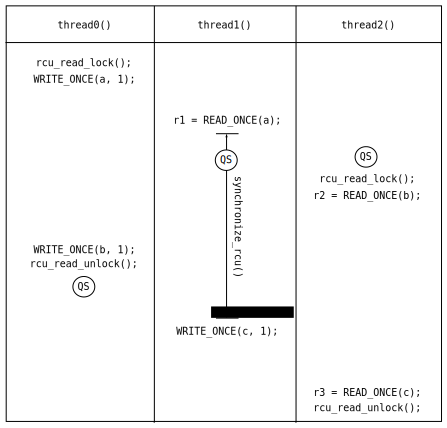
\includegraphics{rcu/design/GPpartitionReaders1}}
\end{center}

If it is necessary to partition RCU read-side critical sections in this
manner, it is necessary to use two grace periods, where the first grace
period is known to end before the second grace period starts:

\begin{VerbatimN}
	void thread0(void)
	{
		rcu_read_lock();
		WRITE_ONCE(a, 1);
		WRITE_ONCE(b, 1);
		rcu_read_unlock();
	}

	void thread1(void)
	{
		r1 = READ_ONCE(a);
		synchronize_rcu();
		WRITE_ONCE(c, 1);
	}

	void thread2(void)
	{
		r2 = READ_ONCE(c);
		synchronize_rcu();
		WRITE_ONCE(d, 1);
	}

	void thread3(void)
	{
		rcu_read_lock();
		r3 = READ_ONCE(b);
		r4 = READ_ONCE(d);
		rcu_read_unlock();
	}
\end{VerbatimN}

Here, if \co{(r1 == 1)}, then \co{thread0()}'s write to~\co{b} must happen
before the end of \co{thread1()}'s grace period.
If in addition
\co{(r4 == 1)}, then \co{thread3()}'s read from~\co{b} must happen after
the beginning of \co{thread2()}'s grace period.
If it is also the case
that \co{(r2 == 1)}, then the end of \co{thread1()}'s grace period must
precede the beginning of \co{thread2()}'s grace period.
This mean that
the two RCU read-side critical sections cannot overlap, guaranteeing
that \co{(r3 == 1)}.
As a result, the outcome:

\begin{VerbatimU}
      (r1 == 1 && r2 == 1 && r3 == 0 && r4 == 1)
\end{VerbatimU}

\noindent%
cannot happen.

This non-requirement was also non-premeditated, but became apparent when
studying RCU's interaction with memory ordering.


\subsubsection{Read-Side Critical Sections Don't Partition Grace Periods}

It is also tempting to assume that if an RCU read-side critical section
happens between a pair of grace periods, then those grace periods cannot
overlap.
However, this temptation leads nowhere good, as can be
illustrated by the following, with all variables initially zero:

\begin{VerbatimN}
	void thread0(void)
	{
		rcu_read_lock();
		WRITE_ONCE(a, 1);
		WRITE_ONCE(b, 1);
		rcu_read_unlock();
	}

	void thread1(void)
	{
		r1 = READ_ONCE(a);
		synchronize_rcu();
		WRITE_ONCE(c, 1);
	}

	void thread2(void)
	{
		rcu_read_lock();
		WRITE_ONCE(d, 1);
		r2 = READ_ONCE(c);
		rcu_read_unlock();
	}

	void thread3(void)
	{
		r3 = READ_ONCE(d);
		synchronize_rcu();
		WRITE_ONCE(e, 1);
	}

	void thread4(void)
	{
		rcu_read_lock();
		r4 = READ_ONCE(b);
		r5 = READ_ONCE(e);
		rcu_read_unlock();
	}
\end{VerbatimN}

In this case, the outcome:

\begin{VerbatimU}
      (r1 == 1 && r2 == 1 && r3 == 1 && r4 == 0 && r5 == 1)
\end{VerbatimU}

\noindent%
is entirely possible, as illustrated below:

\begin{center}
\resizebox{\columnwidth}{!}{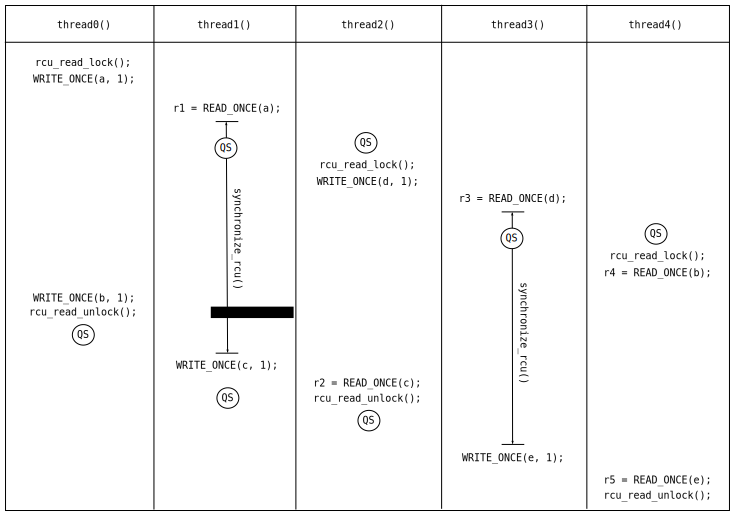
\includegraphics{rcu/design/ReadersPartitionGP1}}
\end{center}

Again, an RCU read-side critical section can overlap almost all of a
given grace period, just so long as it does not overlap the entire grace
period.
As a result, an RCU read-side critical section cannot partition
a pair of RCU grace periods.

\QuickQuiz{
  How long a sequence of grace periods, each separated by an RCU
  read-side critical section, would be required to partition the RCU
  read-side critical sections at the beginning and end of the chain?
}\QuickQuizAnswer{
  In theory, an infinite number. In practice, an unknown number that is
  sensitive to both implementation details and timing considerations.
  Therefore, even in practice, RCU users must abide by the theoretical
  rather than the practical answer.
}\QuickQuizEnd


\subsection{Parallelism Facts of Life}

These parallelism facts of life are by no means specific to RCU, but the
RCU implementation must abide by them.
They therefore bear repeating:

\begin{enumerate}
\item Any CPU or task may be delayed at any time, and any attempts to avoid
   these delays by disabling preemption, interrupts, or whatever are
   completely futile.
   This is most obvious in preemptible user-level
   environments and in virtualized environments (where a given guest
   OS's VCPUs can be preempted at any time by the underlying
   hypervisor), but can also happen in bare-metal environments due to
   ECC errors, NMIs, and other hardware events.
   Although a delay of more
   than about 20~seconds can result in splats, the RCU implementation is
   obligated to use algorithms that can tolerate extremely long delays,
   but where ``extremely long'' is not long enough to allow wrap-around
   when incrementing a 64-bit counter.
\item Both the compiler and the CPU can reorder memory accesses.
   Where it
   matters, RCU must use compiler directives and memory-barrier
   instructions to preserve ordering.
\item Conflicting writes to memory locations in any given cache line will
   result in expensive cache misses.
   Greater numbers of concurrent
   writes and more-frequent concurrent writes will result in more
   dramatic slowdowns.
   RCU is therefore obligated to use algorithms that
   have sufficient locality to avoid significant performance and
   scalability problems.
\item As a rough rule of thumb, only one CPU's worth of processing may be
   carried out under the protection of any given exclusive lock.
   RCU
   must therefore use scalable locking designs.
\item Counters are finite, especially on 32-bit systems.
   RCU's use of
   counters must therefore tolerate counter wrap, or be designed such
   that counter wrap would take way more time than a single system is
   likely to run.
   An uptime of ten years is quite possible, a runtime of
   a century much less so.
   As an example of the latter, RCU's
   dyntick-idle nesting counter allows 54~bits for interrupt nesting
   level (this counter is 64~bits even on a 32-bit system).
   Overflowing
   this counter requires $2^54$ half-interrupts on a given CPU
   without that CPU ever going idle.
   If a half-interrupt happened every
   microsecond, it would take 570 years of runtime to overflow this
   counter, which is currently believed to be an acceptably long time.
\item Linux systems can have thousands of CPUs running a single Linux
   kernel in a single shared-memory environment.
   RCU must therefore pay
   close attention to high-end scalability.
\end{enumerate}

This last parallelism fact of life means that RCU must pay special
attention to the preceding facts of life.
The idea that Linux might
scale to systems with thousands of CPUs would have been met with some
skepticism in the 1990s, but these requirements would have otherwise
have been unsurprising, even in the early 1990s.


\subsection{Quality-of-Implementation Requirements}

These sections list quality-of-implementation requirements.
Although an
RCU implementation that ignores these requirements could still be used,
it would likely be subject to limitations that would make it
inappropriate for industrial-strength production use.
Classes of
quality-of-implementation requirements are as follows:

\begin{enumerate}
\item Specialization
\item Performance and Scalability
\item Forward Progress
\item Composability
\item Corner Cases
\end{enumerate}

These classes is covered in the following sections.


\subsubsection{Specialization}

RCU is and always has been intended primarily for read-mostly
situations, which means that RCU's read-side primitives are optimized,
often at the expense of its update-side primitives.
Experience thus far
is captured by the following list of situations:

\begin{enumerate}
\item Read-mostly data, where stale and inconsistent data is not a problem:
   RCU works great!
\item Read-mostly data, where data must be consistent: RCU works well.
\item Read-write data, where data must be consistent: RCU \emph{might} work OK.
   Or not.
\item Write-mostly data, where data must be consistent: RCU is very
   unlikely to be the right tool for the job, with the following
   exceptions, where RCU can provide:

   \begin{enumerate}
   \item Existence guarantees for update-friendly mechanisms.
   \item Wait-free read-side primitives for real-time use.
   \end{enumerate}
\end{enumerate}

This focus on read-mostly situations means that RCU must interoperate
with other synchronization primitives.
For example, the \co{add_gp()} and
\co{remove_gp_synchronous()} examples discussed earlier use RCU to
protect readers and locking to coordinate updaters.
However, the need
extends much farther, requiring that a variety of synchronization
primitives be legal within RCU read-side critical sections, including
spinlocks, sequence locks, atomic operations, reference counters, and
memory barriers.

\QuickQuiz{
  What about sleeping locks?
}\QuickQuizAnswer{
  These are forbidden within Linux-kernel RCU read-side critical
  sections because it is not legal to place a quiescent state (in this
  case, voluntary context switch) within an RCU read-side critical
  section.
  However, sleeping locks may be used within userspace RCU
  read-side critical sections, and also within Linux-kernel sleepable
  RCU (SRCU) %`(SRCU) <Sleepable RCU_>`__
  read-side critical sections.
  In
  addition, the \co{-rt} patchset turns spinlocks into a sleeping locks so
  that the corresponding critical sections can be preempted, which also
  means that these sleeplockified spinlocks (but not other sleeping
  locks!) may be acquire within \co{-rt}-Linux-kernel RCU read-side critical
  sections.
  Note that it \emph{is} legal for a normal RCU read-side critical section
  to conditionally acquire a sleeping locks (as in
  \co{mutex_trylock()}), but only as long as it does not loop
  indefinitely attempting to conditionally acquire that sleeping locks.
  The key point is that things like \co{mutex_trylock()} either return
  with the mutex held, or return an error indication if the mutex was
  not immediately available. Either way, \co{mutex_trylock()} returns
  immediately without sleeping.
}\QuickQuizEnd

It often comes as a surprise that many algorithms do not require a
consistent view of data, but many can function in that mode, with
network routing being the poster child.
Internet routing algorithms take
significant time to propagate updates, so that by the time an update
arrives at a given system, that system has been sending network traffic
the wrong way for a considerable length of time.
Having a few threads
continue to send traffic the wrong way for a few more milliseconds is
clearly not a problem:
In the worst case, TCP retransmissions will
eventually get the data where it needs to go.
In general, when tracking
the state of the universe outside of the computer, some level of
inconsistency must be tolerated due to speed-of-light delays if nothing
else.

Furthermore, uncertainty about external state is inherent in many cases.
For example, a pair of veterinarians might use heartbeat to determine
whether or not a given cat was alive.
But how long should they wait
after the last heartbeat to decide that the cat is in fact dead?
Waiting
less than 400 milliseconds makes no sense because this would mean that a
relaxed cat would be considered to cycle between death and life more
than 100 times per minute.
Moreover, just as with human beings, a cat's
heart might stop for some period of time, so the exact wait period is a
judgment call.
One of our pair of veterinarians might wait 30 seconds
before pronouncing the cat dead, while the other might insist on waiting
a full minute.
The two veterinarians would then disagree on the state of
the cat during the final 30 seconds of the minute following the last
heartbeat.

Interestingly enough, this same situation applies to hardware.
When push
comes to shove, how do we tell whether or not some external server has
failed?
We send messages to it periodically, and declare it failed if we
don't receive a response within a given period of time.
Policy decisions
can usually tolerate short periods of inconsistency.
The policy was
decided some time ago, and is only now being put into effect, so a few
milliseconds of delay is normally inconsequential.

However, there are algorithms that absolutely must see consistent data.
For example, the translation between a user-level SystemV semaphore ID
to the corresponding in-kernel data structure is protected by RCU, but
it is absolutely forbidden to update a semaphore that has just been
removed.
In the Linux kernel, this need for consistency is accommodated
by acquiring spinlocks located in the in-kernel data structure from
within the RCU read-side critical section, and this is indicated by the
green box in the figure above. Many other techniques may be used, and
are in fact used within the Linux kernel.

In short, RCU is not required to maintain consistency, and other
mechanisms may be used in concert with RCU when consistency is required.
RCU's specialization allows it to do its job extremely well, and its
ability to interoperate with other synchronization mechanisms allows the
right mix of synchronization tools to be used for a given job.


\subsubsection{Performance and Scalability}

Energy efficiency is a critical component of performance today, and
Linux-kernel RCU implementations must therefore avoid unnecessarily
awakening idle CPUs.
I cannot claim that this requirement was
premeditated.
In fact, I learned of it during a telephone conversation
in which I was given ``frank and open'' feedback on the importance of
energy efficiency in battery-powered systems and on specific
energy-efficiency shortcomings of the Linux-kernel RCU implementation.
In my experience, the battery-powered embedded community will consider
any unnecessary wakeups to be extremely unfriendly acts.
So much so that
mere Linux-kernel-mailing-list posts are insufficient to vent their ire.

Memory consumption is not particularly important for in most situations,
and has become decreasingly so as memory sizes have expanded and memory
costs have plummeted.
However, as I learned from Matt Mackall's
\href{http://elinux.org/Linux_Tiny-FAQ}{bloatwatch} efforts, memory
footprint is critically important on single-CPU systems with
non-preemptible (\co{CONFIG_PREEMPTION=n}) kernels, and thus
\href{https://lore.kernel.org/r/20090113221724.GA15307@linux.vnet.ibm.com}{tiny RCU}
was born.
Josh Triplett has since taken over the small-memory banner
with his \href{https://tiny.wiki.kernel.org/}{Linux kernel tinification}
project, which resulted in SRCU %`SRCU <Sleepable RCU_>`__
becoming optional
for those kernels not needing it.

The remaining performance requirements are, for the most part,
unsurprising.
For example, in keeping with RCU's read-side
specialization, \co{rcu_dereference()} should have negligible overhead
(for example, suppression of a few minor compiler optimizations).
Similarly, in non-preemptible environments, \co{rcu_read_lock()} and
\co{rcu_read_unlock()} should have exactly zero overhead.

In preemptible environments, in the case where the RCU read-side
critical section was not preempted (as will be the case for the
highest-priority real-time process), \co{rcu_read_lock()} and
\co{rcu_read_unlock()} should have minimal overhead.
In particular, they
should not contain atomic read-modify-write operations, memory-barrier
instructions, preemption disabling, interrupt disabling, or backwards
branches.
However, in the case where the RCU read-side critical section
was preempted, \co{rcu_read_unlock()} may acquire spinlocks and disable
interrupts.
This is why it is better to nest an RCU read-side critical
section within a preempt-disable region than vice versa, at least in
cases where that critical section is short enough to avoid unduly
degrading real-time latencies.

The \co{synchronize_rcu()} grace-period-wait primitive is optimized for
throughput.
It may therefore incur several milliseconds of latency in
addition to the duration of the longest RCU read-side critical section.
On the other hand, multiple concurrent invocations of
\co{synchronize_rcu()} are required to use batching optimizations so that
they can be satisfied by a single underlying grace-period-wait
operation.
For example, in the Linux kernel, it is not unusual for a
single grace-period-wait operation to serve more than
\href{https://www.usenix.org/conference/2004-usenix-annual-technical-conference/making-rcu-safe-deep-sub-millisecond-response}{1,000 separate invocations}
of \co{synchronize_rcu()}, thus amortizing the per-invocation overhead
down to nearly zero.
However, the grace-period optimization is also
required to avoid measurable degradation of real-time scheduling and
interrupt latencies.

In some cases, the multi-millisecond \co{synchronize_rcu()} latencies are
unacceptable.
In these cases, \co{synchronize_rcu_expedited()} may be
used instead, reducing the grace-period latency down to a few tens of
microseconds on small systems, at least in cases where the RCU read-side
critical sections are short.
There are currently no special latency
requirements for \co{synchronize_rcu_expedited()} on large systems, but,
consistent with the empirical nature of the RCU specification, that is
subject to change.
However, there most definitely are scalability
requirements:
A storm of \co{synchronize_rcu_expedited()} invocations on
4096 CPUs should at least make reasonable forward progress.
In return
for its shorter latencies, \co{synchronize_rcu_expedited()} is permitted
to impose modest degradation of real-time latency on non-idle online
CPUs.
Here, ``modest'' means roughly the same latency degradation as a
scheduling-clock interrupt.

There are a number of situations where even
\co{synchronize_rcu_expedited()}'s reduced grace-period latency is
unacceptable.
In these situations, the \co{asynchronous call_rcu()} can
be used in place of \co{synchronize_rcu()} as follows:

\begin{fcvlabel}[ln:rcu:design:req7]
\begin{VerbatimN}[commandchars=\%\@\$]
	struct foo {          %lnlbl@foo:b$
		int a;
		int b;
		struct rcu_head rh;
	};                    %lnlbl@foo:e$

	static void remove_gp_cb(struct rcu_head *rhp)
	{
		struct foo *p = container_of(rhp, struct foo, rh);

		kfree(p);
	}

	bool remove_gp_asynchronous(void)
	{
		struct foo *p;

		spin_lock(&gp_lock);            %lnlbl@lock$
		p = rcu_access_pointer(gp);     %lnlbl@access$
		if (!p) {
			spin_unlock(&gp_lock);
			return false;
		}
		rcu_assign_pointer(gp, NULL);
		call_rcu(&p->rh, remove_gp_cb);  %lnlbl@call$
		spin_unlock(&gp_lock);           %lnlbl@unlock$
		return true;
	}
\end{VerbatimN}
\end{fcvlabel}

\begin{fcvref}[ln:rcu:design:req7]
A definition of \co{struct foo} is finally needed, and appears on
\clnrefrange{foo:b}{foo:e}. % lines 1-5
The function \co{remove_gp_cb()} is passed to \co{call_rcu()}
on \clnref{call}, % line 25
and will be invoked after the end of a subsequent grace
period.
This gets the same effect as \co{remove_gp_synchronous()}, but
without forcing the updater to wait for a grace period to elapse.
The
\co{call_rcu()} function may be used in a number of situations where
neither \co{synchronize_rcu()} nor \co{synchronize_rcu_expedited()} would
be legal, including within preempt-disable code, \co{local_bh_disable()}
code, interrupt-disable code, and interrupt handlers.
However, even
\co{call_rcu()} is illegal within NMI handlers and from idle and offline
CPUs.
The callback function (\co{remove_gp_cb()} in this case) will be
executed within softirq (software interrupt) environment within the
Linux kernel, either within a real softirq handler or under the
protection of \co{local_bh_disable()}.
In both the Linux kernel and in
userspace, it is bad practice to write an RCU callback function that
takes too long.
Long-running operations should be relegated to separate
threads or (in the Linux kernel) workqueues.
\end{fcvref}

\QuickQuiz{
\begin{fcvref}[ln:rcu:design:req7]
  Why does \clnref{access} % line 19
  use \co{rcu_access_pointer()}? After all,
  \co{call_rcu()} on \clnref{call} % line 25
  stores into the structure, which would
  interact badly with concurrent insertions.
  Doesn't this mean that
  \co{rcu_dereference()} is required?
\end{fcvref}
}\QuickQuizAnswer{
\begin{fcvref}[ln:rcu:design:req7]
  Presumably the \co{->gp_lock} acquired on \clnref{lock} % line 18
  excludes any
  changes, including any insertions that \co{rcu_dereference()} would
  protect against.
  Therefore, any insertions will be delayed until
  after \co{->gp_lock} is released on \clnref{unlock}, % line 26
  which in turn means that
  \co{rcu_access_pointer()} suffices.
\end{fcvref}
}\QuickQuizEnd

However, all that \co{remove_gp_cb()} is doing is invoking \co{kfree()} on
the data element.
This is a common idiom, and is supported by
\co{kfree_rcu()}, which allows ``fire and forget'' operation as shown
below:

\begin{VerbatimN}
	struct foo {
		int a;
		int b;
		struct rcu_head rh;
	};

	bool remove_gp_faf(void)
	{
		struct foo *p;

		spin_lock(&gp_lock);
		p = rcu_dereference(gp);
		if (!p) {
			spin_unlock(&gp_lock);
			return false;
		}
		rcu_assign_pointer(gp, NULL);
		kfree_rcu(p, rh);
		spin_unlock(&gp_lock);
		return true;
	}
\end{VerbatimN}

Note that \co{remove_gp_faf()} simply invokes \co{kfree_rcu()} and
proceeds, without any need to pay any further attention to the
subsequent grace period and \co{kfree()}.
It is permissible to invoke
\co{kfree_rcu()} from the same environments as for \co{call_rcu()}.
Interestingly enough, DYNIX/ptx had the equivalents of \co{call_rcu()}
and \co{kfree_rcu()}, but not \co{synchronize_rcu()}.
This was due to the
fact that RCU was not heavily used within DYNIX/ptx, so the very few
places that needed something like \co{synchronize_rcu()} simply
open-coded it.

\QuickQuiz{
  Earlier it was claimed that \co{call_rcu()} and \co{kfree_rcu()}
  allowed updaters to avoid being blocked by readers.
  But how can that
  be correct, given that the invocation of the callback and the freeing
  of the memory (respectively) must still wait for a grace period to
  elapse?
}\QuickQuizAnswer{
  We could define things this way, but keep in mind that this sort of
  definition would say that updates in garbage-collected languages
  cannot complete until the next time the garbage collector runs, which
  does not seem at all reasonable.
  The key point is that in most cases,
  an updater using either \co{call_rcu()} or \co{kfree_rcu()} can proceed
  to the next update as soon as it has invoked \co{call_rcu()} or
  \co{kfree_rcu()}, without having to wait for a subsequent grace
  period.
}\QuickQuizEnd

But what if the updater must wait for the completion of code to be
executed after the end of the grace period, but has other tasks that can
be carried out in the meantime? The polling-style
\co{get_state_synchronize_rcu()} and \co{cond_synchronize_rcu()} functions
may be used for this purpose, as shown below:

\begin{fcvlabel}[ln:rcu:design:req8]
\begin{VerbatimN}[commandchars=\%\@\$]
	bool remove_gp_poll(void)
	{
		struct foo *p;
		unsigned long s;

		spin_lock(&gp_lock);
		p = rcu_access_pointer(gp);
		if (!p) {
			spin_unlock(&gp_lock);
			return false;
		}
		rcu_assign_pointer(gp, NULL);
		spin_unlock(&gp_lock);
		s = get_state_synchronize_rcu();  %lnlbl@getstate$
		do_something_while_waiting();     %lnlbl@do$
		cond_synchronize_rcu(s);          %lnlbl@condsync$
		kfree(p);
		return true;
	}
\end{VerbatimN}
\end{fcvlabel}

\begin{fcvref}[ln:rcu:design:req8]
On \clnref{getstate}, % line 14
\co{get_state_synchronize_rcu()} obtains a ``cookie'' from RCU,
then \clnref{do} % line 15
carries out other tasks, and finally, \clnref{condsync} % line 16
returns
immediately if a grace period has elapsed in the meantime, but otherwise
waits as required.
\end{fcvref}
The need for \co{get_state_synchronize_rcu} and
\co{cond_synchronize_rcu()} has appeared quite recently, so it is too
early to tell whether they will stand the test of time.

RCU thus provides a range of tools to allow updaters to strike the
required tradeoff between latency, flexibility and CPU overhead.


\subsubsection{Forward Progress}

In theory, delaying grace-period completion and callback invocation is
harmless.
In practice, not only are memory sizes finite but also
callbacks sometimes do wakeups, and sufficiently deferred wakeups can be
difficult to distinguish from system hangs.
Therefore, RCU must provide
a number of mechanisms to promote forward progress.

These mechanisms are not foolproof, nor can they be. For one simple
example, an infinite loop in an RCU read-side critical section must by
definition prevent later grace periods from ever completing.
For a more
involved example, consider a 64-CPU system built with
\co{CONFIG_RCU_NOCB_CPU=y} and booted with \co{rcu_nocbs=1-63}, where
CPUs~1 through~63 spin in tight loops that invoke \co{call_rcu()}.
Even
if these tight loops also contain calls to \co{cond_resched()} (thus
allowing grace periods to complete), CPU~0 simply will not be able to
invoke callbacks as fast as the other 63 CPUs can register them, at
least not until the system runs out of memory.
In both of these
examples, the Spiderman principle applies:
With great power comes great
responsibility.
However, short of this level of abuse, RCU is required
to ensure timely completion of grace periods and timely invocation of
callbacks.

RCU takes the following steps to encourage timely completion of grace
periods:

\begin{enumerate}
\item If a grace period fails to complete within 100 milliseconds, RCU
   causes future invocations of \co{cond_resched()} on the holdout CPUs
   to provide an RCU quiescent state.
   RCU also causes those CPUs'
   \co{need_resched()} invocations to return \co{true}, but only after the
   corresponding CPU's next scheduling-clock.
\item CPUs mentioned in the \co{nohz_full} kernel boot parameter can run
   indefinitely in the kernel without scheduling-clock interrupts, which
   defeats the above \co{need_resched()} strategem.
   RCU will therefore
   invoke \co{resched_cpu()} on any \co{nohz_full} CPUs still holding out
   after 109 milliseconds.
\item In kernels built with \co{CONFIG_RCU_BOOST=y}, if a given task that
   has been preempted within an RCU read-side critical section is
   holding out for more than 500 milliseconds, RCU will resort to
   priority boosting.
\item If a CPU is still holding out 10 seconds into the grace period, RCU
   will invoke \co{resched_cpu()} on it regardless of its \co{nohz_full}
   state.
\end{enumerate}

The above values are defaults for systems running with \co{HZ=1000}.
They
will vary as the value of \co{HZ} varies, and can also be changed using
the relevant Kconfig options and kernel boot parameters.
RCU currently
does not do much sanity checking of these parameters, so please use
caution when changing them.
Note that these forward-progress measures
are provided only for RCU, not for SRCU %`SRCU <Sleepable RCU_>`__
or Task RCU\@. %`Tasks RCU`_.

RCU takes the following steps in \co{call_rcu()} to encourage timely
invocation of callbacks when any given non-\co{rcu_nocbs} CPU has
10,000 callbacks, or has 10,000 more callbacks than it had the last time
encouragement was provided:

\begin{enumerate}
\item Starts a grace period, if one is not already in progress.
\item Forces immediate checking for quiescent states, rather than waiting
   for three milliseconds to have elapsed since the beginning of the
   grace period.
\item Immediately tags the CPU's callbacks with their grace period
   completion numbers, rather than waiting for the \co{RCU_SOFTIRQ}
   handler to get around to it.
\item Lifts callback-execution batch limits, which speeds up callback
   invocation at the expense of degrading realtime response.
\end{enumerate}

Again, these are default values when running at \co{HZ=1000}, and can be
overridden.
Again, these forward-progress measures are provided only for
RCU, not for SRCU %`SRCU <Sleepable RCU_>`__
or Task RCU. %`Tasks RCU`_
Even for RCU, callback-invocation forward
progress for \co{rcu_nocbs} CPUs is much less well-developed, in part
because workloads benefiting from \co{rcu_nocbs} CPUs tend to invoke
\co{call_rcu()} relatively infrequently.
If workloads emerge that need
both \co{rcu_nocbs} CPUs and high \co{call_rcu()} invocation rates, then
additional forward-progress work will be required.


\subsubsection{Composability}

Composability has received much attention in recent years, perhaps in
part due to the collision of multicore hardware with object-oriented
techniques designed in single-threaded environments for single-threaded
use.
And in theory, RCU read-side critical sections may be composed, and
in fact may be nested arbitrarily deeply.
In practice, as with all
real-world implementations of composable constructs, there are
limitations.

Implementations of RCU for which \co{rcu_read_lock()} and
\co{rcu_read_unlock()} generate no code, such as Linux-kernel RCU when
\co{CONFIG_PREEMPTION=n}, can be nested arbitrarily deeply.
After all, there
is no overhead. Except that if all these instances of
\co{rcu_read_lock()} and \co{rcu_read_unlock()} are visible to the
compiler, compilation will eventually fail due to exhausting memory,
mass storage, or user patience, whichever comes first.
If the nesting is
not visible to the compiler, as is the case with mutually recursive
functions each in its own translation unit, stack overflow will result.
If the nesting takes the form of loops, perhaps in the guise of tail
recursion, either the control variable will overflow or (in the Linux
kernel) you will get an RCU CPU stall warning. Nevertheless, this class
of RCU implementations is one of the most composable constructs in
existence.

RCU implementations that explicitly track nesting depth are limited by
the nesting-depth counter.
For example, the Linux kernel's preemptible
RCU limits nesting to \co{INT_MAX}. This should suffice for almost all
practical purposes.
That said, a consecutive pair of RCU read-side
critical sections between which there is an operation that waits for a
grace period cannot be enclosed in another RCU read-side critical
section.
This is because it is not legal to wait for a grace period
within an RCU read-side critical section:
To do so would result either
in deadlock or in RCU implicitly splitting the enclosing RCU read-side
critical section, neither of which is conducive to a long-lived and
prosperous kernel.

It is worth noting that RCU is not alone in limiting composability. For
example, many transactional-memory implementations prohibit composing a
pair of transactions separated by an irrevocable operation (for example,
a network receive operation).
For another example, lock-based critical
sections can be composed surprisingly freely, but only if deadlock is
avoided.

In short, although RCU read-side critical sections are highly
composable, care is required in some situations, just as is the case for
any other composable synchronization mechanism.


\subsubsection{Corner Cases}

A given RCU workload might have an endless and intense stream of RCU
read-side critical sections, perhaps even so intense that there was
never a point in time during which there was not at least one RCU
read-side critical section in flight.
RCU cannot allow this situation to
block grace periods: As long as all the RCU read-side critical sections
are finite, grace periods must also be finite.

That said, preemptible RCU implementations could potentially result in
RCU read-side critical sections being preempted for long durations,
which has the effect of creating a long-duration RCU read-side critical
section.
This situation can arise only in heavily loaded systems, but
systems using real-time priorities are of course more vulnerable.
Therefore, RCU priority boosting is provided to help deal with this
case.
That said, the exact requirements on RCU priority boosting will
likely evolve as more experience accumulates.

Other workloads might have very high update rates.
Although one can
argue that such workloads should instead use something other than RCU,
the fact remains that RCU must handle such workloads gracefully.
This
requirement is another factor driving batching of grace periods, but it
is also the driving force behind the checks for large numbers of queued
RCU callbacks in the \co{call_rcu()} code path.
Finally, high update
rates should not delay RCU read-side critical sections, although some
small read-side delays can occur when using
\co{synchronize_rcu_expedited()}, courtesy of this function's use of
\co{smp_call_function_single()}.

Although all three of these corner cases were understood in the early
1990s, a simple user-level test consisting of \co{close(open(path))} in a
tight loop in the early 2000s suddenly provided a much deeper
appreciation of the high-update-rate corner case.
This test also
motivated addition of some RCU code to react to high update rates, for
example, if a given CPU finds itself with more than 10,000 RCU callbacks
queued, it will cause RCU to take evasive action by more aggressively
starting grace periods and more aggressively forcing completion of
grace-period processing.
This evasive action causes the grace period to
complete more quickly, but at the cost of restricting RCU's batching
optimizations, thus increasing the CPU overhead incurred by that grace
period.


\subsection{Software-Engineering Requirements}

Between Murphy's Law and ``To err is human'', it is necessary to guard
against mishaps and misuse:

\begin{enumerate}
\item It is all too easy to forget to use \co{rcu_read_lock()} everywhere
   that it is needed, so kernels built with \co{CONFIG_PROVE_RCU=y} will
   splat if \co{rcu_dereference()} is used outside of an RCU read-side
   critical section.
   Update-side code can use
   \co{rcu_dereference_protected()}, which takes a
   \href{https://lwn.net/Articles/371986/}{lockdep expression} to indicate what is
   providing the protection.
   If the indicated protection is not
   provided, a lockdep splat is emitted.
   Code shared between readers and updaters can use
   \co{rcu_dereference_check()}, which also takes a lockdep expression,
   and emits a lockdep splat if neither \co{rcu_read_lock()} nor the
   indicated protection is in place.
   In addition,
   \co{rcu_dereference_raw()} is used in those (hopefully rare) cases
   where the required protection cannot be easily described.
   Finally,
   \co{rcu_read_lock_held()} is provided to allow a function to verify
   that it has been invoked within an RCU read-side critical section.
   I
   was made aware of this set of requirements shortly after Thomas
   Gleixner audited a number of RCU uses.
\item A given function might wish to check for RCU-related preconditions
   upon entry, before using any other RCU API\@.
   The
   \co{rcu_lockdep_assert()} does this job, asserting the expression in
   kernels having lockdep enabled and doing nothing otherwise.
\item It is also easy to forget to use \co{rcu_assign_pointer()} and
   \co{rcu_dereference()}, perhaps (incorrectly) substituting a simple
   assignment.
   To catch this sort of error, a given RCU-protected
   pointer may be tagged with \co{__rcu}, after which \co{sparse} will
   complain about simple-assignment accesses to that pointer.
   Arnd
   Bergmann made me aware of this requirement, and also supplied the
   needed \href{https://lwn.net/Articles/376011/}{patch series}.
\item Kernels built with \co{CONFIG_DEBUG_OBJECTS_RCU_HEAD=y} will splat if
   a data element is passed to \co{call_rcu()} twice in a row, without a
   grace period in between.
   (This error is similar to a double free.)
   The corresponding \co{rcu_head} structures that are dynamically
   allocated are automatically tracked, but \co{rcu_head} structures
   allocated on the stack must be initialized with
   \co{init_rcu_head_on_stack()} and cleaned up with
   \co{destroy_rcu_head_on_stack()}.
   Similarly, statically allocated
   non-stack \co{rcu_head} structures must be initialized with
   \co{init_rcu_head()} and cleaned up with \co{destroy_rcu_head()}.
   Mathieu Desnoyers made me aware of this requirement, and also
   supplied the needed
   \href{https://lore.kernel.org/r/20100319013024.GA28456@Krystal}{patch}.
\item An infinite loop in an RCU read-side critical section will eventually
   trigger an RCU CPU stall warning splat, with the duration of
   ``eventually'' being controlled by the \co{RCU_CPU_STALL_TIMEOUT}
   \co{Kconfig} option, or, alternatively, by the
   \co{rcupdate.rcu_cpu_stall_timeout} boot/sysfs parameter.
   However, RCU
   is not obligated to produce this splat unless there is a grace period
   waiting on that particular RCU read-side critical section.

   Some extreme workloads might intentionally delay RCU grace periods,
   and systems running those workloads can be booted with
   \co{rcupdate.rcu_cpu_stall_suppress} to suppress the splats.
   This
   kernel parameter may also be set via \co{sysfs}. Furthermore, RCU CPU
   stall warnings are counter-productive during sysrq dumps and during
   panics.
   RCU therefore supplies the \co{rcu_sysrq_start()} and
   \co{rcu_sysrq_end()} API members to be called before and after long
   sysrq dumps.
   RCU also supplies the \co{rcu_panic()} notifier that is
   automatically invoked at the beginning of a panic to suppress further
   RCU CPU stall warnings.

   This requirement made itself known in the early 1990s, pretty much
   the first time that it was necessary to debug a CPU stall. That said,
   the initial implementation in DYNIX/ptx was quite generic in
   comparison with that of Linux.

\item Although it would be very good to detect pointers leaking out of RCU
   read-side critical sections, there is currently no good way of doing
   this.
   One complication is the need to distinguish between pointers
   leaking and pointers that have been handed off from RCU to some other
   synchronization mechanism, for example, reference counting.
\item In kernels built with \co{CONFIG_RCU_TRACE=y}, RCU-related information
   is provided via event tracing.
\item Open-coded use of \co{rcu_assign_pointer()} and \co{rcu_dereference()}
   to create typical linked data structures can be surprisingly
   error-prone. Therefore, RCU-protected
   \href{https://lwn.net/Articles/609973/#RCU%20List%20APIs}{linked lists} and,
   more recently, RCU-protected
   \href{https://lwn.net/Articles/612100/}{hash tables} are available.
   Many
   other special-purpose RCU-protected data structures are available in
   the Linux kernel and the userspace RCU library.
\item Some linked structures are created at compile time, but still require
   \co{__rcu} checking.
   The \co{RCU_POINTER_INITIALIZER()} macro serves
   this purpose.
\item It is not necessary to use \co{rcu_assign_pointer()} when creating
   linked structures that are to be published via a single external
   pointer.
   The \co{RCU_INIT_POINTER()} macro is provided for this task.
\end{enumerate}

This not a hard-and-fast list:
RCU's diagnostic capabilities will
continue to be guided by the number and type of usage bugs found in
real-world RCU usage.


\subsection{Linux Kernel Complications}

The Linux kernel provides an interesting environment for all kinds of
software, including RCU\@.
Some of the relevant points of interest are as
follows:

\begin{enumerate}
\item Configuration
\item Firmware Interface
\item Early Boot
\item Interrupts and NMIs
\item Loadable Modules
\item Hotplug CPU
\item Scheduler and RCU
\item Tracing and RCU
\item Accesses to User Memory and RCU
\item Energy Efficiency
\item Scheduling-Clock Interrupts and RCU
\item Memory Efficiency
\item Performance, Scalability, Response Time, and Reliability
\end{enumerate}

This list is probably incomplete, but it does give a feel for the most
notable Linux-kernel complications.
Each of the following sections
covers one of the above topics.


\subsubsection{Configuration}

RCU's goal is automatic configuration, so that almost nobody needs to
worry about RCU's \co{Kconfig} options.
And for almost all users, RCU
does in fact work well ``out of the box.''

However, there are specialized use cases that are handled by kernel boot
parameters and \co{Kconfig} options.
Unfortunately, the \co{Kconfig}
system will explicitly ask users about new \co{Kconfig} options, which
requires almost all of them be hidden behind a \co{CONFIG_RCU_EXPERT}
\co{Kconfig} option.

This all should be quite obvious, but the fact remains that Linus
Torvalds recently had to
\href{https://lore.kernel.org/r/CA+55aFy4wcCwaL4okTs8wXhGZ5h-ibecy_Meg9C4MNQrUnwMcg@mail.gmail.com>}{remind}
me of this requirement.


\subsubsection{Firmware Interface}

In many cases, kernel obtains information about the system from the
firmware, and sometimes things are lost in translation.
Or the
translation is accurate, but the original message is bogus.

For example, some systems' firmware overreports the number of CPUs,
sometimes by a large factor.
If RCU naively believed the firmware, as it
used to do, it would create too many per-CPU kthreads.
Although the
resulting system will still run correctly, the extra kthreads needlessly
consume memory and can cause confusion when they show up in \co{ps}
listings.

RCU must therefore wait for a given CPU to actually come online before
it can allow itself to believe that the CPU actually exists.
The
resulting ``ghost CPUs'' (which are never going to come online) cause a
number of \href{https://paulmck.livejournal.com/37494.html}{interesting complications}.


\subsubsection{Early Boot}

The Linux kernel's boot sequence is an interesting process, and RCU is
used early, even before \co{rcu_init()} is invoked.
In fact, a number of
RCU's primitives can be used as soon as the initial task's
\co{task_struct} is available and the boot CPU's per-CPU variables are
set up.
The read-side primitives (\co{rcu_read_lock()},
\co{rcu_read_unlock()}, \co{rcu_dereference()}, and
\co{rcu_access_pointer()}) will operate normally very early on, as will
\co{rcu_assign_pointer()}.

Although \co{call_rcu()} may be invoked at any time during boot,
callbacks are not guaranteed to be invoked until after all of RCU's
kthreads have been spawned, which occurs at \co{early_initcall()} time.
This delay in callback invocation is due to the fact that RCU does not
invoke callbacks until it is fully initialized, and this full
initialization cannot occur until after the scheduler has initialized
itself to the point where RCU can spawn and run its kthreads.
In theory,
it would be possible to invoke callbacks earlier, however, this is not a
panacea because there would be severe restrictions on what operations
those callbacks could invoke.

Perhaps surprisingly, \co{synchronize_rcu()} and
\co{synchronize_rcu_expedited()}, will operate normally during very early
boot, the reason being that there is only one CPU and preemption is
disabled.
This means that the call \co{synchronize_rcu()} (or friends)
itself is a quiescent state and thus a grace period, so the early-boot
implementation can be a no-op.

However, once the scheduler has spawned its first kthread, this early
boot trick fails for \co{synchronize_rcu()} (as well as for
\co{synchronize_rcu_expedited()}) in \co{CONFIG_PREEMPTION=y} kernels.
The
reason is that an RCU read-side critical section might be preempted,
which means that a subsequent \co{synchronize_rcu()} really does have to
wait for something, as opposed to simply returning immediately.
Unfortunately, \co{synchronize_rcu()} can't do this until all of its
kthreads are spawned, which doesn't happen until some time during
\co{early_initcalls()} time. But this is no excuse:
RCU is nevertheless
required to correctly handle synchronous grace periods during this time
period.
Once all of its kthreads are up and running, RCU starts running
normally.

\QuickQuiz{
  How can RCU possibly handle grace periods before all of its kthreads
  have been spawned???
}\QuickQuizAnswer{
  Very carefully!
  During the ``dead zone'' between the time that the scheduler spawns the
  first task and the time that all of RCU's kthreads have been spawned,
  all synchronous grace periods are handled by the expedited
  grace-period mechanism.
  At runtime, this expedited mechanism relies
  on workqueues, but during the dead zone the requesting task itself
  drives the desired expedited grace period.
  Because dead-zone
  execution takes place within task context, everything works.
  Once the
  dead zone ends, expedited grace periods go back to using workqueues,
  as is required to avoid problems that would otherwise occur when a
  user task received a POSIX signal while driving an expedited grace
  period.

  And yes, this does mean that it is unhelpful to send POSIX signals to
  random tasks between the time that the scheduler spawns its first
  kthread and the time that RCU's kthreads have all been spawned.
  If
  there ever turns out to be a good reason for sending POSIX signals
  during that time, appropriate adjustments will be made.
  (If it turns
  out that POSIX signals are sent during this time for no good reason,
  other adjustments will be made, appropriate or otherwise.)
}\QuickQuizEnd

I learned of these boot-time requirements as a result of a series of
system hangs.


\subsubsection{Interrupts and NMIs}

The Linux kernel has interrupts, and RCU read-side critical sections are
legal within interrupt handlers and within interrupt-disabled regions of
code, as are invocations of \co{call_rcu()}.

Some Linux-kernel architectures can enter an interrupt handler from
non-idle process context, and then just never leave it, instead
stealthily transitioning back to process context.
This trick is
sometimes used to invoke system calls from inside the kernel. These
``half-interrupts'' mean that RCU has to be very careful about how it
counts interrupt nesting levels.
I learned of this requirement the hard
way during a rewrite of RCU's dyntick-idle code.

The Linux kernel has non-maskable interrupts (NMIs), and RCU read-side
critical sections are legal within NMI handlers.
Thankfully, RCU
update-side primitives, including \co{call_rcu()}, are prohibited within
NMI handlers.

The name notwithstanding, some Linux-kernel architectures can have
nested NMIs, which RCU must handle correctly. Andy Lutomirski
\href{https://lore.kernel.org/r/CALCETrXLq1y7e_dKFPgou-FKHB6Pu-r8+t-6Ds+8=va7anBWDA@mail.gmail.com}{surprised me}
with this requirement; he also kindly surprised me with
\href{https://lore.kernel.org/r/CALCETrXSY9JpW3uE6H8WYk81sg56qasA2aqmjMPsq5dOtzso=g@mail.gmail.com}{an algorithm}
that meets this requirement.

Furthermore, NMI handlers can be interrupted by what appear to RCU to be
normal interrupts.
One way that this can happen is for code that
directly invokes \co{ct_irq_enter()} and \co{ct_irq_exit()} to be called
from an NMI handler.
This astonishing fact of life prompted the current
code structure, which has \co{ct_irq_enter()} invoking
\co{ct_nmi_enter()} and \co{ct_irq_exit()} invoking \co{ct_nmi_exit()}.
And yes, I also learned of this requirement the hard way.


\subsubsection{Loadable Modules}

The Linux kernel has loadable modules, and these modules can also be
unloaded.
After a given module has been unloaded, any attempt to call
one of its functions results in a segmentation fault.
The module-unload
functions must therefore cancel any delayed calls to loadable-module
functions, for example, any outstanding \co{mod_timer()} must be dealt
with via \co{timer_shutdown_sync()} or similar.

Unfortunately, there is no way to cancel an RCU callback; once you
invoke \co{call_rcu()}, the callback function is eventually going to be
invoked, unless the system goes down first.
Because it is normally
considered socially irresponsible to crash the system in response to a
module unload request, we need some other way to deal with in-flight RCU
callbacks.

RCU therefore provides \co{rcu_barrier()}, which waits until all
in-flight RCU callbacks have been invoked.
If a module uses
\co{call_rcu()}, its exit function should therefore prevent any future
invocation of \co{call_rcu()}, then invoke \co{rcu_barrier()}.
In theory,
the underlying module-unload code could invoke \co{rcu_barrier()}
unconditionally, but in practice this would incur unacceptable
latencies.

Nikita Danilov noted this requirement for an analogous
filesystem-unmount situation, and Dipankar Sarma incorporated
\co{rcu_barrier()} into RCU\@.
The need for \co{rcu_barrier()} for module
unloading became apparent later.

\begin{Note}
   important:

   The \co{rcu_barrier()} function is not, repeat,
   \emph{not}, obligated to wait for a grace period.
   It is instead only required
   to wait for RCU callbacks that have already been posted.
   Therefore, if
   there are no RCU callbacks posted anywhere in the system,
   \co{rcu_barrier()} is within its rights to return immediately.
   Even if
   there are callbacks posted, \co{rcu_barrier()} does not necessarily need
   to wait for a grace period.
\end{Note}

\QuickQuiz{
  Wait a minute!
  Each RCU callbacks must wait for a grace period to
  complete, and \co{rcu_barrier()} must wait for each pre-existing
  callback to be invoked.
  Doesn't \co{rcu_barrier()} therefore need to
  wait for a full grace period if there is even one callback posted
  anywhere in the system?
}\QuickQuizAnswer{
  Absolutely not!!!
  Yes, each RCU callbacks must wait for a grace period to complete, but
  it might well be partly (or even completely) finished waiting by the
  time \co{rcu_barrier()} is invoked.
  In that case, \co{rcu_barrier()}
  need only wait for the remaining portion of the grace period to
  elapse.
  So even if there are quite a few callbacks posted,
  \co{rcu_barrier()} might well return quite quickly.

  So if you need to wait for a grace period as well as for all
  pre-existing callbacks, you will need to invoke both
  \co{synchronize_rcu()} and \co{rcu_barrier()}.
  If latency is a concern,
  you can always use workqueues to invoke them concurrently.
}\QuickQuizEnd


\subsubsection{Hotplug CPU}

The Linux kernel supports CPU hotplug, which means that CPUs can come
and go.
It is of course illegal to use any RCU API member from an
offline CPU, with the exception of SRCU % `SRCU <Sleepable RCU_>`__
read-side
critical sections.
This requirement was present from day one in
DYNIX/ptx, but on the other hand, the Linux kernel's CPU-hotplug
implementation is ``interesting.''

The Linux-kernel CPU-hotplug implementation has notifiers that are used
to allow the various kernel subsystems (including RCU) to respond
appropriately to a given CPU-hotplug operation.
Most RCU operations may
be invoked from CPU-hotplug notifiers, including even synchronous
grace-period operations such as (\co{synchronize_rcu()} and
\co{synchronize_rcu_expedited()}).
However, these synchronous operations
do block and therefore cannot be invoked from notifiers that execute via
\co{stop_machine()}, specifically those between the \co{CPUHP_AP_OFFLINE}
and \co{CPUHP_AP_ONLINE} states.

In addition, all-callback-wait operations such as \co{rcu_barrier()} may
not be invoked from any CPU-hotplug notifier.
This restriction is due
to the fact that there are phases of CPU-hotplug operations where the
outgoing CPU's callbacks will not be invoked until after the CPU-hotplug
operation ends, which could also result in deadlock.
Furthermore,
\co{rcu_barrier()} blocks CPU-hotplug operations during its execution,
which results in another type of deadlock when invoked from a CPU-hotplug
notifier.

Finally, RCU must avoid deadlocks due to interaction between hotplug,
timers and grace period processing.
It does so by maintaining its own set
of books that duplicate the centrally maintained \co{cpu_online_mask},
and also by reporting quiescent states explicitly when a CPU goes
offline.
This explicit reporting of quiescent states avoids any need
for the force-quiescent-state loop (FQS) to report quiescent states for
offline CPUs.
However, as a debugging measure, the FQS loop does splat
if offline CPUs block an RCU grace period for too long.

An offline CPU's quiescent state will be reported either:

\begin{enumerate}
\item  As the CPU goes offline using RCU's hotplug notifier (\co{rcutree_report_cpu_dead()}).
\item  When grace period initialization (\co{rcu_gp_init()}) detects a
    race either with CPU offlining or with a task unblocking on a leaf
    \co{rcu_node} structure whose CPUs are all offline.
\end{enumerate}

The CPU-online path (\co{rcutree_report_cpu_starting()}) should never need to report
a quiescent state for an offline CPU\@.
However, as a debugging measure,
it does emit a warning if a quiescent state was not already reported
for that CPU\@.

During the checking/modification of RCU's hotplug bookkeeping, the
corresponding CPU's leaf node lock is held.
This avoids race conditions
between RCU's hotplug notifier hooks, the grace period initialization
code, and the FQS loop, all of which refer to or modify this bookkeeping.


\subsubsection{Scheduler and RCU}

RCU makes use of kthreads, and it is necessary to avoid excessive CPU-time
accumulation by these kthreads.
This requirement was no surprise, but
RCU's violation of it when running context-switch-heavy workloads when
built with \co{CONFIG_NO_HZ_FULL=y}
\href{http://www.rdrop.com/users/paulmck/scalability/paper/BareMetal.2015.01.15b.pdf}{did come as a surprise [PDF]}.
RCU has made good progress towards meeting this requirement, even for
context-switch-heavy \co{CONFIG_NO_HZ_FULL=y} workloads, but there is
room for further improvement.

There is no longer any prohibition against holding any of
scheduler's runqueue or priority-inheritance spinlocks across an
\co{rcu_read_unlock()}, even if interrupts and preemption were enabled
somewhere within the corresponding RCU read-side critical section.
Therefore, it is now perfectly legal to execute \co{rcu_read_lock()}
with preemption enabled, acquire one of the scheduler locks, and hold
that lock across the matching \co{rcu_read_unlock()}.

Similarly, the RCU flavor consolidation has removed the need for negative
nesting.
The fact that interrupt-disabled regions of code act as RCU
read-side critical sections implicitly avoids earlier issues that used
to result in destructive recursion via interrupt handler's use of RCU\@.


\subsubsection{Tracing and RCU}

It is possible to use tracing on RCU code, but tracing itself uses RCU\@.
For this reason, \co{rcu_dereference_raw_check()} is provided for use
by tracing, which avoids the destructive recursion that could otherwise
ensue.
This API is also used by virtualization in some architectures,
where RCU readers execute in environments in which tracing cannot be
used.
The tracing folks both located the requirement and provided the
needed fix, so this surprise requirement was relatively painless.


\subsubsection{Accesses to User Memory and RCU}

The kernel needs to access user-space memory, for example, to access data
referenced by system-call parameters.
The \co{get_user()} macro does this job.

However, user-space memory might well be paged out, which means that
\co{get_user()} might well page-fault and thus block while waiting for the
resulting I/O to complete.
It would be a very bad thing for the compiler to
reorder a \co{get_user()} invocation into an RCU read-side critical section.

For example, suppose that the source code looked like this:

\begin{VerbatimN}
	rcu_read_lock();
	p = rcu_dereference(gp);
	v = p->value;
	rcu_read_unlock();
	get_user(user_v, user_p);
	do_something_with(v, user_v);
\end{VerbatimN}

The compiler must not be permitted to transform this source code into
the following:

\begin{fcvlabel}[ln:rcu:design:req9]
\begin{VerbatimN}[commandchars=\%\@\$]
	rcu_read_lock();
	p = rcu_dereference(gp);
	get_user(user_v, user_p); // BUG: POSSIBLE PAGE FAULT!!!
	v = p->value;     %lnlbl@uaf$
	rcu_read_unlock();
	do_something_with(v, user_v);
\end{VerbatimN}
\end{fcvlabel}

If the compiler did make this transformation in a \co{CONFIG_PREEMPTION=n} kernel
build, and if \co{get_user()} did page fault, the result would be a quiescent
state in the middle of an RCU read-side critical section.
\begin{fcvref}[ln:rcu:design:req9]
This misplaced
quiescent state could result in \clnref{uaf} % line 4
being a use-after-free access,
which could be bad for your kernel's actuarial statistics.
Similar examples
can be constructed with the call to \co{get_user()} preceding the
\co{rcu_read_lock()}.
\end{fcvref}

Unfortunately, \co{get_user()} doesn't have any particular ordering properties,
and in some architectures the underlying \co{asm} isn't even marked
\co{volatile}.
And even if it was marked \co{volatile}, the above access to
\co{p->value} is not volatile, so the compiler would not have any reason to keep
those two accesses in order.

Therefore, the Linux-kernel definitions of \co{rcu_read_lock()} and
\co{rcu_read_unlock()} must act as compiler barriers, at least for outermost
instances of \co{rcu_read_lock()} and \co{rcu_read_unlock()} within a nested set
of RCU read-side critical sections.


\subsubsection{Energy Efficiency}

Interrupting idle CPUs is considered socially unacceptable, especially
by people with battery-powered embedded systems.
RCU therefore conserves
energy by detecting which CPUs are idle, including tracking CPUs that
have been interrupted from idle.
This is a large part of the
energy-efficiency requirement, so I learned of this via an irate phone
call.

Because RCU avoids interrupting idle CPUs, it is illegal to execute an
RCU read-side critical section on an idle CPU.
(Kernels built with
\co{CONFIG_PROVE_RCU=y} will splat if you try it.)

It is similarly socially unacceptable to interrupt an \co{nohz_full} CPU
running in userspace.
RCU must therefore track \co{nohz_full} userspace
execution.
RCU must therefore be able to sample state at two points in
time, and be able to determine whether or not some other CPU spent any
time idle and/or executing in userspace.

These energy-efficiency requirements have proven quite difficult to
understand and to meet, for example, there have been more than five
clean-sheet rewrites of RCU's energy-efficiency code, the last of which
was finally able to demonstrate
\href{http://www.rdrop.com/users/paulmck/realtime/paper/AMPenergy.2013.04.19a.pdf}{real energy savings running on real hardware [PDF]}.
As noted earlier, I learned of many of these requirements via angry
phone calls:
Flaming me on the Linux-kernel mailing list was apparently
not sufficient to fully vent their ire at RCU's energy-efficiency bugs!


\subsubsection{Scheduling-Clock Interrupts and RCU}

The kernel transitions between in-kernel non-idle execution, userspace
execution, and the idle loop.
Depending on kernel configuration, RCU
handles these states differently:

\begin{VerbatimU}
+-------------+------------------+------------------+-----------------+
| HZ Kconfig  | In-Kernel        | Usermode         | Idle            |
+=============+==================+==================+=================+
| HZ_PERIODIC | Can rely on      | Can rely on      | Can rely on     |
|             | scheduling-clock | scheduling-clock | RCU's           |
|             | interrupt.       | interrupt and    | dyntick-idle    |
|             |                  | its detection    | detection.      |
|             |                  | of interrupt     |                 |
|             |                  | from usermode.   |                 |
+-------------+------------------+------------------+-----------------+
| NO_HZ_IDLE  | Can rely on      | Can rely on      | Can rely on     |
|             | scheduling-clock | scheduling-clock | RCU's           |
|             | interrupt.       | interrupt and    | dyntick-idle    |
|             |                  | its detection    | detection.      |
|             |                  | of interrupt     |                 |
|             |                  | from usermode.   |                 |
+-------------+------------------+------------------+-----------------+
| NO_HZ_FULL  | Can only         | Can rely on      | Can rely on     |
|             | sometimes rely   | RCU's            | RCU's           |
|             | on               | dyntick-idle     | dyntick-idle    |
|             | scheduling-clock | detection.       | detection.      |
|             | interrupt. In    |                  |                 |
|             | other cases, it  |                  |                 |
|             | is necessary to  |                  |                 |
|             | bound kernel     |                  |                 |
|             | execution times  |                  |                 |
|             | and/or use       |                  |                 |
|             | IPIs.            |                  |                 |
+-------------+------------------+------------------+-----------------+
\end{VerbatimU}

\QuickQuiz{
  Why can't \co{NO_HZ_FULL} in-kernel execution rely on the
  scheduling-clock interrupt, just like \co{HZ_PERIODIC} and
  \co{NO_HZ_IDLE} do?
}\QuickQuizAnswer{
  Because, as a performance optimization, \co{NO_HZ_FULL} does not
  necessarily re-enable the scheduling-clock interrupt on entry to each
  and every system call.
}\QuickQuizEnd

However, RCU must be reliably informed as to whether any given CPU is
currently in the idle loop, and, for \co{NO_HZ_FULL}, also whether that
CPU is executing in usermode, as discussed earlier. % `earlier <Energy Efficiency_>`__.
It also requires that the
scheduling-clock interrupt be enabled when RCU needs it to be:

\begin{enumerate}
\item If a CPU is either idle or executing in usermode, and RCU believes it
   is non-idle, the scheduling-clock tick had better be running.
   Otherwise, you will get RCU CPU stall warnings.
   Or at best, very long
   (11-second) grace periods, with a pointless IPI waking the CPU from
   time to time.
\item If a CPU is in a portion of the kernel that executes RCU read-side
   critical sections, and RCU believes this CPU to be idle, you will get
   random memory corruption.
   \textbf{DON'T DO THIS!!!}
   This is one reason to test with lockdep, which will complain about
   this sort of thing.
\item If a CPU is in a portion of the kernel that is absolutely positively
   no-joking guaranteed to never execute any RCU read-side critical
   sections, and RCU believes this CPU to be idle, no problem.
   This
   sort of thing is used by some architectures for light-weight
   exception handlers, which can then avoid the overhead of
   \co{ct_irq_enter()} and \co{ct_irq_exit()} at exception entry and
   exit, respectively.
   Some go further and avoid the entireties of
   \co{irq_enter()} and \co{irq_exit()}.
   Just make very sure you are running some of your tests with
   \co{CONFIG_PROVE_RCU=y}, just in case one of your code paths was in
   fact joking about not doing RCU read-side critical sections.
\item If a CPU is executing in the kernel with the scheduling-clock
   interrupt disabled and RCU believes this CPU to be non-idle, and if
   the CPU goes idle (from an RCU perspective) every few jiffies, no
   problem.
   It is usually OK for there to be the occasional gap between
   idle periods of up to a second or so.
   If the gap grows too long, you get RCU CPU stall warnings.
\item If a CPU is either idle or executing in usermode, and RCU believes it
   to be idle, of course no problem.
\item If a CPU is executing in the kernel, the kernel code path is passing
   through quiescent states at a reasonable frequency (preferably about
   once per few jiffies, but the occasional excursion to a second or so
   is usually OK) and the scheduling-clock interrupt is enabled, of
   course no problem.
   If the gap between a successive pair of quiescent states grows too
   long, you get RCU CPU stall warnings.
\end{enumerate}

\QuickQuiz{
  But what if my driver has a hardware interrupt handler that can run
  for many seconds?
  I cannot invoke \co{schedule()} from an hardware
  interrupt handler, after all!
}\QuickQuizAnswer{
  One approach is to do \co{ct_irq_exit(); ct_irq_enter();} every so
  often.
  But given that long-running interrupt handlers can cause other
  problems, not least for response time, shouldn't you work to keep
  your interrupt handler's runtime within reasonable bounds?
}\QuickQuizEnd

But as long as RCU is properly informed of kernel state transitions
between in-kernel execution, usermode execution, and idle, and as long
as the scheduling-clock interrupt is enabled when RCU needs it to be,
you can rest assured that the bugs you encounter will be in some other
part of RCU or some other part of the kernel!


\subsubsection{Memory Efficiency}

Although small-memory non-realtime systems can simply use Tiny RCU, code
size is only one aspect of memory efficiency.
Another aspect is the size
of the \co{rcu_head} structure used by \co{call_rcu()} and
\co{kfree_rcu()}.
Although this structure contains nothing more than a
pair of pointers, it does appear in many RCU-protected data structures,
including some that are size critical.
The \co{page} structure is a case
in point, as evidenced by the many occurrences of the \co{union} keyword
within that structure.

This need for memory efficiency is one reason that RCU uses hand-crafted
singly linked lists to track the \co{rcu_head} structures that are
waiting for a grace period to elapse.
It is also the reason why
\co{rcu_head} structures do not contain debug information, such as fields
tracking the file and line of the \co{call_rcu()} or \co{kfree_rcu()} that
posted them.
Although this information might appear in debug-only kernel
builds at some point, in the meantime, the \co{->func} field will often
provide the needed debug information.

However, in some cases, the need for memory efficiency leads to even
more extreme measures.
Returning to the \co{page} structure, the
\co{rcu_head} field shares storage with a great many other structures
that are used at various points in the corresponding page's lifetime.
In
order to correctly resolve certain
\href{https://lore.kernel.org/r/1439976106-137226-1-git-send-email-kirill.shutemov@linux.intel.com}{race conditions},
the Linux kernel's memory-management subsystem needs a particular bit to
remain zero during all phases of grace-period processing, and that bit
happens to map to the bottom bit of the \co{rcu_head} structure's
\co{->next} field.
RCU makes this guarantee as long as \co{call_rcu()} is
used to post the callback, as opposed to \co{kfree_rcu()} or some future
``lazy'' variant of \co{call_rcu()} that might one day be created for
energy-efficiency purposes.

That said, there are limits.
RCU requires that the \co{rcu_head}
structure be aligned to a two-byte boundary, and passing a misaligned
\co{rcu_head} structure to one of the \co{call_rcu()} family of functions
will result in a splat.
It is therefore necessary to exercise caution
when packing structures containing fields of type \co{rcu_head}.
Why not
a four-byte or even eight-byte alignment requirement?
Because the m68k
architecture provides only two-byte alignment, and thus acts as
alignment's least common denominator.

The reason for reserving the bottom bit of pointers to \co{rcu_head}
structures is to leave the door open to ``lazy'' callbacks whose
invocations can safely be deferred. Deferring invocation could
potentially have energy-efficiency benefits, but only if the rate of
non-lazy callbacks decreases significantly for some important workload.
In the meantime, reserving the bottom bit keeps this option open in case
it one day becomes useful.


\subsubsection{Performance, Scalability, Response Time, and Reliability}

Expanding on the earlier discussion, % `earlier discussion <Performance and Scalability_>`__
RCU is used heavily by
hot code paths in performance-critical portions of the Linux kernel's
networking, security, virtualization, and scheduling code paths.
RCU
must therefore use efficient implementations, especially in its
read-side primitives.
To that end, it would be good if preemptible RCU's
implementation of \co{rcu_read_lock()} could be inlined, however, doing
this requires resolving \co{#include} issues with the \co{task_struct}
structure.

The Linux kernel supports hardware configurations with up to 4096 CPUs,
which means that RCU must be extremely scalable.
Algorithms that involve
frequent acquisitions of global locks or frequent atomic operations on
global variables simply cannot be tolerated within the RCU
implementation. RCU therefore makes heavy use of a combining tree based
on the \co{rcu_node} structure.
RCU is required to tolerate all CPUs
continuously invoking any combination of RCU's runtime primitives with
minimal per-operation overhead.
In fact, in many cases, increasing load
must \emph{decrease} the per-operation overhead, witness the batching
optimizations for \co{synchronize_rcu()}, \co{call_rcu()},
\co{synchronize_rcu_expedited()}, and \co{rcu_barrier()}.
As a general
rule, RCU must cheerfully accept whatever the rest of the Linux kernel
decides to throw at it.

The Linux kernel is used for real-time workloads, especially in
conjunction with the
\href{https://wiki.linuxfoundation.org/realtime/}{\co{-rt} patchset}.
The
real-time-latency response requirements are such that the traditional
approach of disabling preemption across RCU read-side critical sections
is inappropriate.
Kernels built with \co{CONFIG_PREEMPTION=y} therefore use
an RCU implementation that allows RCU read-side critical sections to be
preempted.
This requirement made its presence known after users made it
clear that an earlier
\href{https://lwn.net/Articles/107930/}{real-time patch}
did not meet their needs, in
conjunction with some
\href{https://lore.kernel.org/r/20050318002026.GA2693@us.ibm.com}{RCU issues}
encountered by a very early version of the \co{-rt} patchset.

In addition, RCU must make do with a sub-100-microsecond real-time
latency budget.
In fact, on smaller systems with the \co{-rt} patchset, the
Linux kernel provides sub-20-microsecond real-time latencies for the
whole kernel, including RCU\@.
RCU's scalability and latency must
therefore be sufficient for these sorts of configurations.
To my
surprise, the sub-100-microsecond real-time latency budget
\href{http://www.rdrop.com/users/paulmck/realtime/paper/bigrt.2013.01.31a.LCA.pdf}{applies to even the largest systems [PDF]},
up to and including systems with 4096 CPUs.
This real-time requirement
motivated the grace-period kthread, which also simplified handling of a
number of race conditions.

RCU must avoid degrading real-time response for CPU-bound threads,
whether executing in usermode (which is one use case for
\co{CONFIG_NO_HZ_FULL=y}) or in the kernel.
That said, CPU-bound loops in
the kernel must execute \co{cond_resched()} at least once per few tens of
milliseconds in order to avoid receiving an IPI from RCU\@.

Finally, RCU's status as a synchronization primitive means that any RCU
failure can result in arbitrary memory corruption that can be extremely
difficult to debug.
This means that RCU must be extremely reliable,
which in practice also means that RCU must have an aggressive
stress-test suite.
This stress-test suite is called \co{rcutorture}.

Although the need for \co{rcutorture} was no surprise, the current
immense popularity of the Linux kernel is posing interesting---and perhaps
unprecedented---validation challenges.
To see this, keep in mind that
there are well over one billion instances of the Linux kernel running
today, given Android smartphones, Linux-powered televisions, and
servers.
This number can be expected to increase sharply with the advent
of the celebrated Internet of Things.

Suppose that RCU contains a race condition that manifests on average
once per million years of runtime.
This bug will be occurring about
three times per \emph{day} across the installed base. RCU could simply hide
behind hardware error rates, given that no one should really expect
their smartphone to last for a million years.
However, anyone taking too
much comfort from this thought should consider the fact that in most
jurisdictions, a successful multi-year test of a given mechanism, which
might include a Linux kernel, suffices for a number of types of
safety-critical certifications.
In fact, rumor has it that the Linux
kernel is already being used in production for safety-critical
applications.
I don't know about you, but I would feel quite bad if a
bug in RCU killed someone.
Which might explain my recent focus on
validation and verification.


\subsection{Other RCU Flavors}

One of the more surprising things about RCU is that there are now no
fewer than five \emph{flavors}, or API families.
In addition, the primary
flavor that has been the sole focus up to this point has two different
implementations, non-preemptible and preemptible.
The other four flavors
are listed below, with requirements for each described in a separate
section.

\begin{enumerate}
\item Bottom-Half Flavor (Historical)
\item Sched Flavor (Historical)
\item Sleepable RCU
\item Tasks RCU
\item Tasks Trace RCU
\end{enumerate}


\subsubsection{Bottom-Half Flavor (Historical)}

The RCU-bh flavor of RCU has since been expressed in terms of the other
RCU flavors as part of a consolidation of the three flavors into a
single flavor.
The read-side API remains, and continues to disable
softirq and to be accounted for by lockdep.
Much of the material in this
section is therefore strictly historical in nature.

The softirq-disable (AKA ``bottom-half'', hence the \qco{_bh} abbreviations)
flavor of RCU, or \emph{RCU-bh}, was developed by Dipankar Sarma to provide a
flavor of RCU that could withstand the network-based denial-of-service
attacks researched by Robert Olsson.
These attacks placed so much
networking load on the system that some of the CPUs never exited softirq
execution, which in turn prevented those CPUs from ever executing a
context switch, which, in the RCU implementation of that time, prevented
grace periods from ever ending.
The result was an out-of-memory
condition and a system hang.

The solution was the creation of RCU-bh, which does
\co{local_bh_disable()} across its read-side critical sections, and which
uses the transition from one type of softirq processing to another as a
quiescent state in addition to context switch, idle, user mode, and
offline.
This means that RCU-bh grace periods can complete even when
some of the CPUs execute in softirq indefinitely, thus allowing
algorithms based on RCU-bh to withstand network-based denial-of-service
attacks.

Because \co{rcu_read_lock_bh()} and \co{rcu_read_unlock_bh()} disable and
re-enable softirq handlers, any attempt to start a softirq handlers
during the RCU-bh read-side critical section will be deferred.
In this
case, \co{rcu_read_unlock_bh()} will invoke softirq processing, which can
take considerable time.
One can of course argue that this softirq
overhead should be associated with the code following the RCU-bh
read-side critical section rather than \co{rcu_read_unlock_bh()}, but the
fact is that most profiling tools cannot be expected to make this sort
of fine distinction.
For example, suppose that a three-millisecond-long
RCU-bh read-side critical section executes during a time of heavy
networking load.
There will very likely be an attempt to invoke at least
one softirq handler during that three milliseconds, but any such
invocation will be delayed until the time of the
\co{rcu_read_unlock_bh()}.
This can of course make it appear at first
glance as if \co{rcu_read_unlock_bh()} was executing very slowly.

The \href{https://lwn.net/Articles/609973/#RCU%20Per-Flavor%20API%20Table}{RCU-bh API}
includes \co{rcu_read_lock_bh()}, \co{rcu_read_unlock_bh()}, \co{rcu_dereference_bh()},
\co{rcu_dereference_bh_check()}, and \co{rcu_read_lock_bh_held()}.
However, the
old RCU-bh update-side APIs are now gone, replaced by \co{synchronize_rcu()},
\co{synchronize_rcu_expedited()}, \co{call_rcu()}, and \co{rcu_barrier()}.
In addition,
anything that disables bottom halves also marks an RCU-bh read-side
critical section, including \co{local_bh_disable()} and \co{local_bh_enable()},
\co{local_irq_save()} and \co{local_irq_restore()}, and so on.


\subsubsection{Sched Flavor (Historical)}

The RCU-sched flavor of RCU has since been expressed in terms of the
other RCU flavors as part of a consolidation of the three flavors into a
single flavor.
The read-side API remains, and continues to disable
preemption and to be accounted for by lockdep.
Much of the material in
this section is therefore strictly historical in nature.

Before preemptible RCU, waiting for an RCU grace period had the side
effect of also waiting for all pre-existing interrupt and NMI handlers.
However, there are legitimate preemptible-RCU implementations that do
not have this property, given that any point in the code outside of an
RCU read-side critical section can be a quiescent state.
Therefore,
\emph{RCU-sched} was created, which follows ``classic'' RCU in that an
RCU-sched grace period waits for pre-existing interrupt and NMI
handlers.
In kernels built with \co{CONFIG_PREEMPTION=n}, the RCU and
RCU-sched APIs have identical implementations, while kernels built with
\co{CONFIG_PREEMPTION=y} provide a separate implementation for each.

Note well that in \co{CONFIG_PREEMPTION=y} kernels,
\co{rcu_read_lock_sched()} and \co{rcu_read_unlock_sched()} disable and
re-enable preemption, respectively.
This means that if there was a
preemption attempt during the RCU-sched read-side critical section,
\co{rcu_read_unlock_sched()} will enter the scheduler, with all the
latency and overhead entailed.
Just as with \co{rcu_read_unlock_bh()},
this can make it look as if \co{rcu_read_unlock_sched()} was executing
very slowly. However, the highest-priority task won't be preempted, so
that task will enjoy low-overhead \co{rcu_read_unlock_sched()}
invocations.

The \href{https://lwn.net/Articles/609973/#RCU%20Per-Flavor%20API%20Table}{RCU-sched API}
includes \co{rcu_read_lock_sched()}, \co{rcu_read_unlock_sched()},
\co{rcu_read_lock_sched_notrace()}, \co{rcu_read_unlock_sched_notrace()},
\co{rcu_dereference_sched()}, \co{rcu_dereference_sched_check()}, and
\co{rcu_read_lock_sched_held()}.
However, the old RCU-sched update-side APIs
are now gone, replaced by \co{synchronize_rcu()}, \co{synchronize_rcu_expedited()},
\co{call_rcu()}, and \co{rcu_barrier()}.
In addition, anything that disables
preemption also marks an RCU-sched read-side critical section,
including \co{preempt_disable()} and \co{preempt_enable()}, \co{local_irq_save()}
and \co{local_irq_restore()}, and so on.


\subsubsection{Sleepable RCU}

For well over a decade, someone saying ``I need to block within an RCU
read-side critical section'' was a reliable indication that this someone
did not understand RCU\@.
After all, if you are always blocking in an RCU
read-side critical section, you can probably afford to use a
higher-overhead synchronization mechanism.
However, that changed with
the advent of the Linux kernel's notifiers, whose RCU read-side critical
sections almost never sleep, but sometimes need to.
This resulted in the
introduction of \href{https://lwn.net/Articles/202847/}{sleepable RCU}, or
\emph{SRCU}.

SRCU allows different domains to be defined, with each such domain
defined by an instance of an \co{srcu_struct} structure.
A pointer to
this structure must be passed in to each SRCU function, for example,
\co{synchronize_srcu(&ss)}, where \co{ss} is the \co{srcu_struct}
structure.
The key benefit of these domains is that a slow SRCU reader
in one domain does not delay an SRCU grace period in some other domain.
That said, one consequence of these domains is that read-side code must
pass a ``cookie'' from \co{srcu_read_lock()} to \co{srcu_read_unlock()}, for
example, as follows:

\begin{VerbatimN}
	int idx;

	idx = srcu_read_lock(&ss);
	do_something();
	srcu_read_unlock(&ss, idx);
\end{VerbatimN}

As noted above, it is legal to block within SRCU read-side critical
sections, however, with great power comes great responsibility.
If you
block forever in one of a given domain's SRCU read-side critical
sections, then that domain's grace periods will also be blocked forever.
Of course, one good way to block forever is to deadlock, which can
happen if any operation in a given domain's SRCU read-side critical
section can wait, either directly or indirectly, for that domain's grace
period to elapse.
For example, this results in a self-deadlock:

\begin{fcvlabel}[ln:rcu:design:req10]
\begin{VerbatimN}[commandchars=\%\@\$]
	int idx;

	idx = srcu_read_lock(&ss);
	do_something();
	synchronize_srcu(&ss);     %lnlbl@syncsrcu$
	srcu_read_unlock(&ss, idx);
\end{VerbatimN}
\end{fcvlabel}

\begin{fcvref}[ln:rcu:design:req10]
However, if \clnref{syncsrcu} % line 5
acquired a mutex that was held across a
\co{synchronize_srcu()} for domain \co{ss}, deadlock would still be
possible.
Furthermore, if \clnref{syncsrcu} % line 5
acquired a mutex that was held across a
\co{synchronize_srcu()} for some other domain \co{ss1}, and if an
\co{ss1}-domain SRCU read-side critical section acquired another mutex
that was held across as \co{ss}-domain \co{synchronize_srcu()}, deadlock
would again be possible.
Such a deadlock cycle could extend across an
arbitrarily large number of different SRCU domains.
Again, with great
power comes great responsibility.
\end{fcvref}

Unlike the other RCU flavors, SRCU read-side critical sections can run
on idle and even offline CPUs.
This ability requires that
\co{srcu_read_lock()} and \co{srcu_read_unlock()} contain memory barriers,
which means that SRCU readers will run a bit slower than would RCU
readers.
It also motivates the \co{smp_mb__after_srcu_read_unlock()} API,
which, in combination with \co{srcu_read_unlock()}, guarantees a full
memory barrier.

Also unlike other RCU flavors, \co{synchronize_srcu()} may \emph{not} be
invoked from CPU-hotplug notifiers, due to the fact that SRCU grace
periods make use of timers and the possibility of timers being
temporarily ``stranded'' on the outgoing CPU\@.
This stranding of timers
means that timers posted to the outgoing CPU will not fire until late in
the CPU-hotplug process.
The problem is that if a notifier is waiting on
an SRCU grace period, that grace period is waiting on a timer, and that
timer is stranded on the outgoing CPU, then the notifier will never be
awakened, in other words, deadlock has occurred.
This same situation of
course also prohibits \co{srcu_barrier()} from being invoked from
CPU-hotplug notifiers.

SRCU also differs from other RCU flavors in that SRCU's expedited and
non-expedited grace periods are implemented by the same mechanism.
This
means that in the current SRCU implementation, expediting a future grace
period has the side effect of expediting all prior grace periods that
have not yet completed.
(But please note that this is a property of the
current implementation, not necessarily of future implementations.)
In
addition, if SRCU has been idle for longer than the interval specified
by the \co{srcutree.exp_holdoff} kernel boot parameter (25 microseconds
by default), and if a \co{synchronize_srcu()} invocation ends this idle
period, that invocation will be automatically expedited.

As of v4.12, SRCU's callbacks are maintained per-CPU, eliminating a
locking bottleneck present in prior kernel versions.
Although this will
allow users to put much heavier stress on \co{call_srcu()}, it is
important to note that SRCU does not yet take any special steps to deal
with callback flooding. So if you are posting (say) 10,000 SRCU
callbacks per second per CPU, you are probably totally OK, but if you
intend to post (say) 1,000,000 SRCU callbacks per second per CPU, please
run some tests first.
SRCU just might need a few adjustment to deal with
that sort of load.
Of course, your mileage may vary based on the speed
of your CPUs and the size of your memory.

The \href{https://lwn.net/Articles/609973/#RCU%20Per-Flavor%20API%20Table}{SRCU API}
includes \co{srcu_read_lock()}, \co{srcu_read_unlock()},
\co{srcu_dereference()}, \co{srcu_dereference_check()},
\co{synchronize_srcu()}, \co{synchronize_srcu_expedited()},
\co{call_srcu()}, \co{srcu_barrier()}, and \co{srcu_read_lock_held()}.
It
also includes \co{DEFINE_SRCU()}, \co{DEFINE_STATIC_SRCU()}, and
\co{init_srcu_struct()} APIs for defining and initializing
\co{srcu_struct} structures.

More recently, the SRCU API has added polling interfaces:

\begin{enumerate}
\item \co{start_poll_synchronize_srcu()} returns a cookie identifying
   the completion of a future SRCU grace period and ensures
   that this grace period will be started.
\item \co{poll_state_synchronize_srcu()} returns \co{true} iff the
   specified cookie corresponds to an already-completed
   SRCU grace period.
\item \co{get_state_synchronize_srcu()} returns a cookie just like
   \co{start_poll_synchronize_srcu()} does, but differs in that
   it does nothing to ensure that any future SRCU grace period
   will be started.
\end{enumerate}

These functions are used to avoid unnecessary SRCU grace periods in
certain types of buffer-cache algorithms having multi-stage age-out
mechanisms.
The idea is that by the time the block has aged completely
from the cache, an SRCU grace period will be very likely to have elapsed.


\subsubsection{Tasks RCU}

Some forms of tracing use ``trampolines'' to handle the binary rewriting
required to install different types of probes.
It would be good to be
able to free old trampolines, which sounds like a job for some form of
RCU\@.
However, because it is necessary to be able to install a trace
anywhere in the code, it is not possible to use read-side markers such
as \co{rcu_read_lock()} and \co{rcu_read_unlock()}.
In addition, it does
not work to have these markers in the trampoline itself, because there
would need to be instructions following \co{rcu_read_unlock()}.
Although
\co{synchronize_rcu()} would guarantee that execution reached the
\co{rcu_read_unlock()}, it would not be able to guarantee that execution
had completely left the trampoline.
Worse yet, in some situations
the trampoline's protection must extend a few instructions \emph{prior} to
execution reaching the trampoline.
For example, these few instructions
might calculate the address of the trampoline, so that entering the
trampoline would be pre-ordained a surprisingly long time before execution
actually reached the trampoline itself.

The solution, in the form of
\href{https://lwn.net/Articles/607117/}{Tasks RCU},
is to have implicit read-side
critical sections that are delimited by voluntary context switches, that
is, calls to \co{schedule()}, \co{cond_resched()}, and
\co{synchronize_rcu_tasks()}.
In addition, transitions to and from
userspace execution also delimit tasks-RCU read-side critical sections.
Idle tasks are ignored by Tasks RCU, and Tasks Rude RCU may be used to
interact with them.

Note well that involuntary context switches are \emph{not} Tasks-RCU quiescent
states.
After all, in preemptible kernels, a task executing code in a
trampoline might be preempted.
In this case, the Tasks-RCU grace period
clearly cannot end until that task resumes and its execution leaves that
trampoline.
This means, among other things, that \co{cond_resched()} does
not provide a Tasks RCU quiescent state.
(Instead, use \co{rcu_softirq_qs()}
from softirq or \co{rcu_tasks_classic_qs()} otherwise.)

The tasks-RCU API is quite compact, consisting only of
\co{call_rcu_tasks()}, \co{synchronize_rcu_tasks()}, and
\co{rcu_barrier_tasks()}.
In \co{CONFIG_PREEMPTION=n} kernels, trampolines
cannot be preempted, so these APIs map to \co{call_rcu()},
\co{synchronize_rcu()}, and \co{rcu_barrier()}, respectively.
In
\co{CONFIG_PREEMPTION=y} kernels, trampolines can be preempted, and these
three APIs are therefore implemented by separate functions that check
for voluntary context switches.


\subsubsection{Tasks Rude RCU}

Some forms of tracing need to wait for all preemption-disabled regions
of code running on any online CPU, including those executed when RCU is
not watching.
This means that \co{synchronize_rcu()} is insufficient, and
Tasks Rude RCU must be used instead.
This flavor of RCU does its work by
forcing a workqueue to be scheduled on each online CPU, hence the ``Rude''
moniker.
And this operation is considered to be quite rude by real-time
workloads that don't want their \co{nohz_full} CPUs receiving IPIs and
by battery-powered systems that don't want their idle CPUs to be awakened.

Once kernel entry/exit and deep-idle functions have been properly tagged
\co{noinstr}`, Tasks RCU can start paying attention to idle tasks (except
those that are idle from RCU's perspective) and then Tasks Rude RCU can
be removed from the kernel.

The tasks-rude-RCU API is also reader-marking-free and thus quite compact,
consisting solely of \co{synchronize_rcu_tasks_rude()}.


\subsubsection{Tasks Trace RCU}

Some forms of tracing need to sleep in readers, but cannot tolerate
SRCU's read-side overhead, which includes a full memory barrier in both
\co{srcu_read_lock()} and \co{srcu_read_unlock()}.
This need is handled by a
Tasks Trace RCU that uses scheduler locking and IPIs to synchronize with
readers.
Real-time systems that cannot tolerate IPIs may build their
kernels with \co{CONFIG_TASKS_TRACE_RCU_READ_MB=y}, which avoids the IPIs at
the expense of adding full memory barriers to the read-side primitives.

The tasks-trace-RCU API is also reasonably compact,
consisting of \co{rcu_read_lock_trace()}, \co{rcu_read_unlock_trace()},
\co{rcu_read_lock_trace_held()}, \co{call_rcu_tasks_trace()},
\co{synchronize_rcu_tasks_trace()}, and \co{rcu_barrier_tasks_trace()}.


\subsection{Possible Future Changes}

One of the tricks that RCU uses to attain update-side scalability is to
increase grace-period latency with increasing numbers of CPUs.
If this
becomes a serious problem, it will be necessary to rework the
grace-period state machine so as to avoid the need for the additional
latency.

RCU disables CPU hotplug in a few places, perhaps most notably in the
\co{rcu_barrier()} operations.
If there is a strong reason to use
\co{rcu_barrier()} in CPU-hotplug notifiers, it will be necessary to
avoid disabling CPU hotplug.
This would introduce some complexity, so
there had better be a \emph{very} good reason.

The tradeoff between grace-period latency on the one hand and
interruptions of other CPUs on the other hand may need to be
re-examined.
The desire is of course for zero grace-period latency as
well as zero interprocessor interrupts undertaken during an expedited
grace period operation.
While this ideal is unlikely to be achievable,
it is quite possible that further improvements can be made.

The multiprocessor implementations of RCU use a combining tree that
groups CPUs so as to reduce lock contention and increase cache locality.
However, this combining tree does not spread its memory across NUMA
nodes nor does it align the CPU groups with hardware features such as
sockets or cores.
Such spreading and alignment is currently believed to
be unnecessary because the hotpath read-side primitives do not access
the combining tree, nor does \co{call_rcu()} in the common case.
If you
believe that your architecture needs such spreading and alignment, then
your architecture should also benefit from the
\co{rcutree.rcu_fanout_leaf} boot parameter, which can be set to the
number of CPUs in a socket, NUMA node, or whatever.
If the number of
CPUs is too large, use a fraction of the number of CPUs.
If the number
of CPUs is a large prime number, well, that certainly is an
``interesting'' architectural choice! More flexible arrangements might be
considered, but only if \co{rcutree.rcu_fanout_leaf} has proven
inadequate, and only if the inadequacy has been demonstrated by a
carefully run and realistic system-level workload.

Please note that arrangements that require RCU to remap CPU numbers will
require extremely good demonstration of need and full exploration of
alternatives.

RCU's various kthreads are reasonably recent additions.
It is quite
likely that adjustments will be required to more gracefully handle
extreme loads.
It might also be necessary to be able to relate CPU
utilization by RCU's kthreads and softirq handlers to the code that
instigated this CPU utilization.
For example, RCU callback overhead
might be charged back to the originating \co{call_rcu()} instance, though
probably not in production kernels.

Additional work may be required to provide reasonable forward-progress
guarantees under heavy load for grace periods and for callback
invocation.


\subsection{Summary}

This document has presented more than two decade's worth of RCU
requirements.
Given that the requirements keep changing, this will not
be the last word on this subject, but at least it serves to get an
important subset of the requirements set forth.


\subsection{Acknowledgments}

I am grateful to Steven Rostedt, Lai Jiangshan, Ingo Molnar, Oleg
Nesterov, Borislav Petkov, Peter Zijlstra, Boqun Feng, and Andy
Lutomirski for their help in rendering this article human readable, and
to Michelle Rankin for her support of this effort.
Other contributions
are acknowledged in the Linux kernel's git archive.

%\section{A Tour Through Tree RCU's Data Structures [LWN.net]}
\label{sec:rcu:A Tour Through Tree RCU's Data Structures}

\begin{Note}
December 18, 2016

This article was contributed by Paul E. McKenney
\end{Note}

\subsection{Introduction}

This document describes RCU's major data structures and their relationship
to each other.

\subsection{Data-Structure Relationships}

RCU is for all intents and purposes a large state machine, and its
data structures maintain the state in such a way as to allow RCU readers
to execute extremely quickly, while also processing the RCU grace periods
requested by updaters in an efficient and extremely scalable fashion.
The efficiency and scalability of RCU updaters is provided primarily
by a combining tree, as shown below:

\begin{center}
\resizebox{.7\columnwidth}{!}{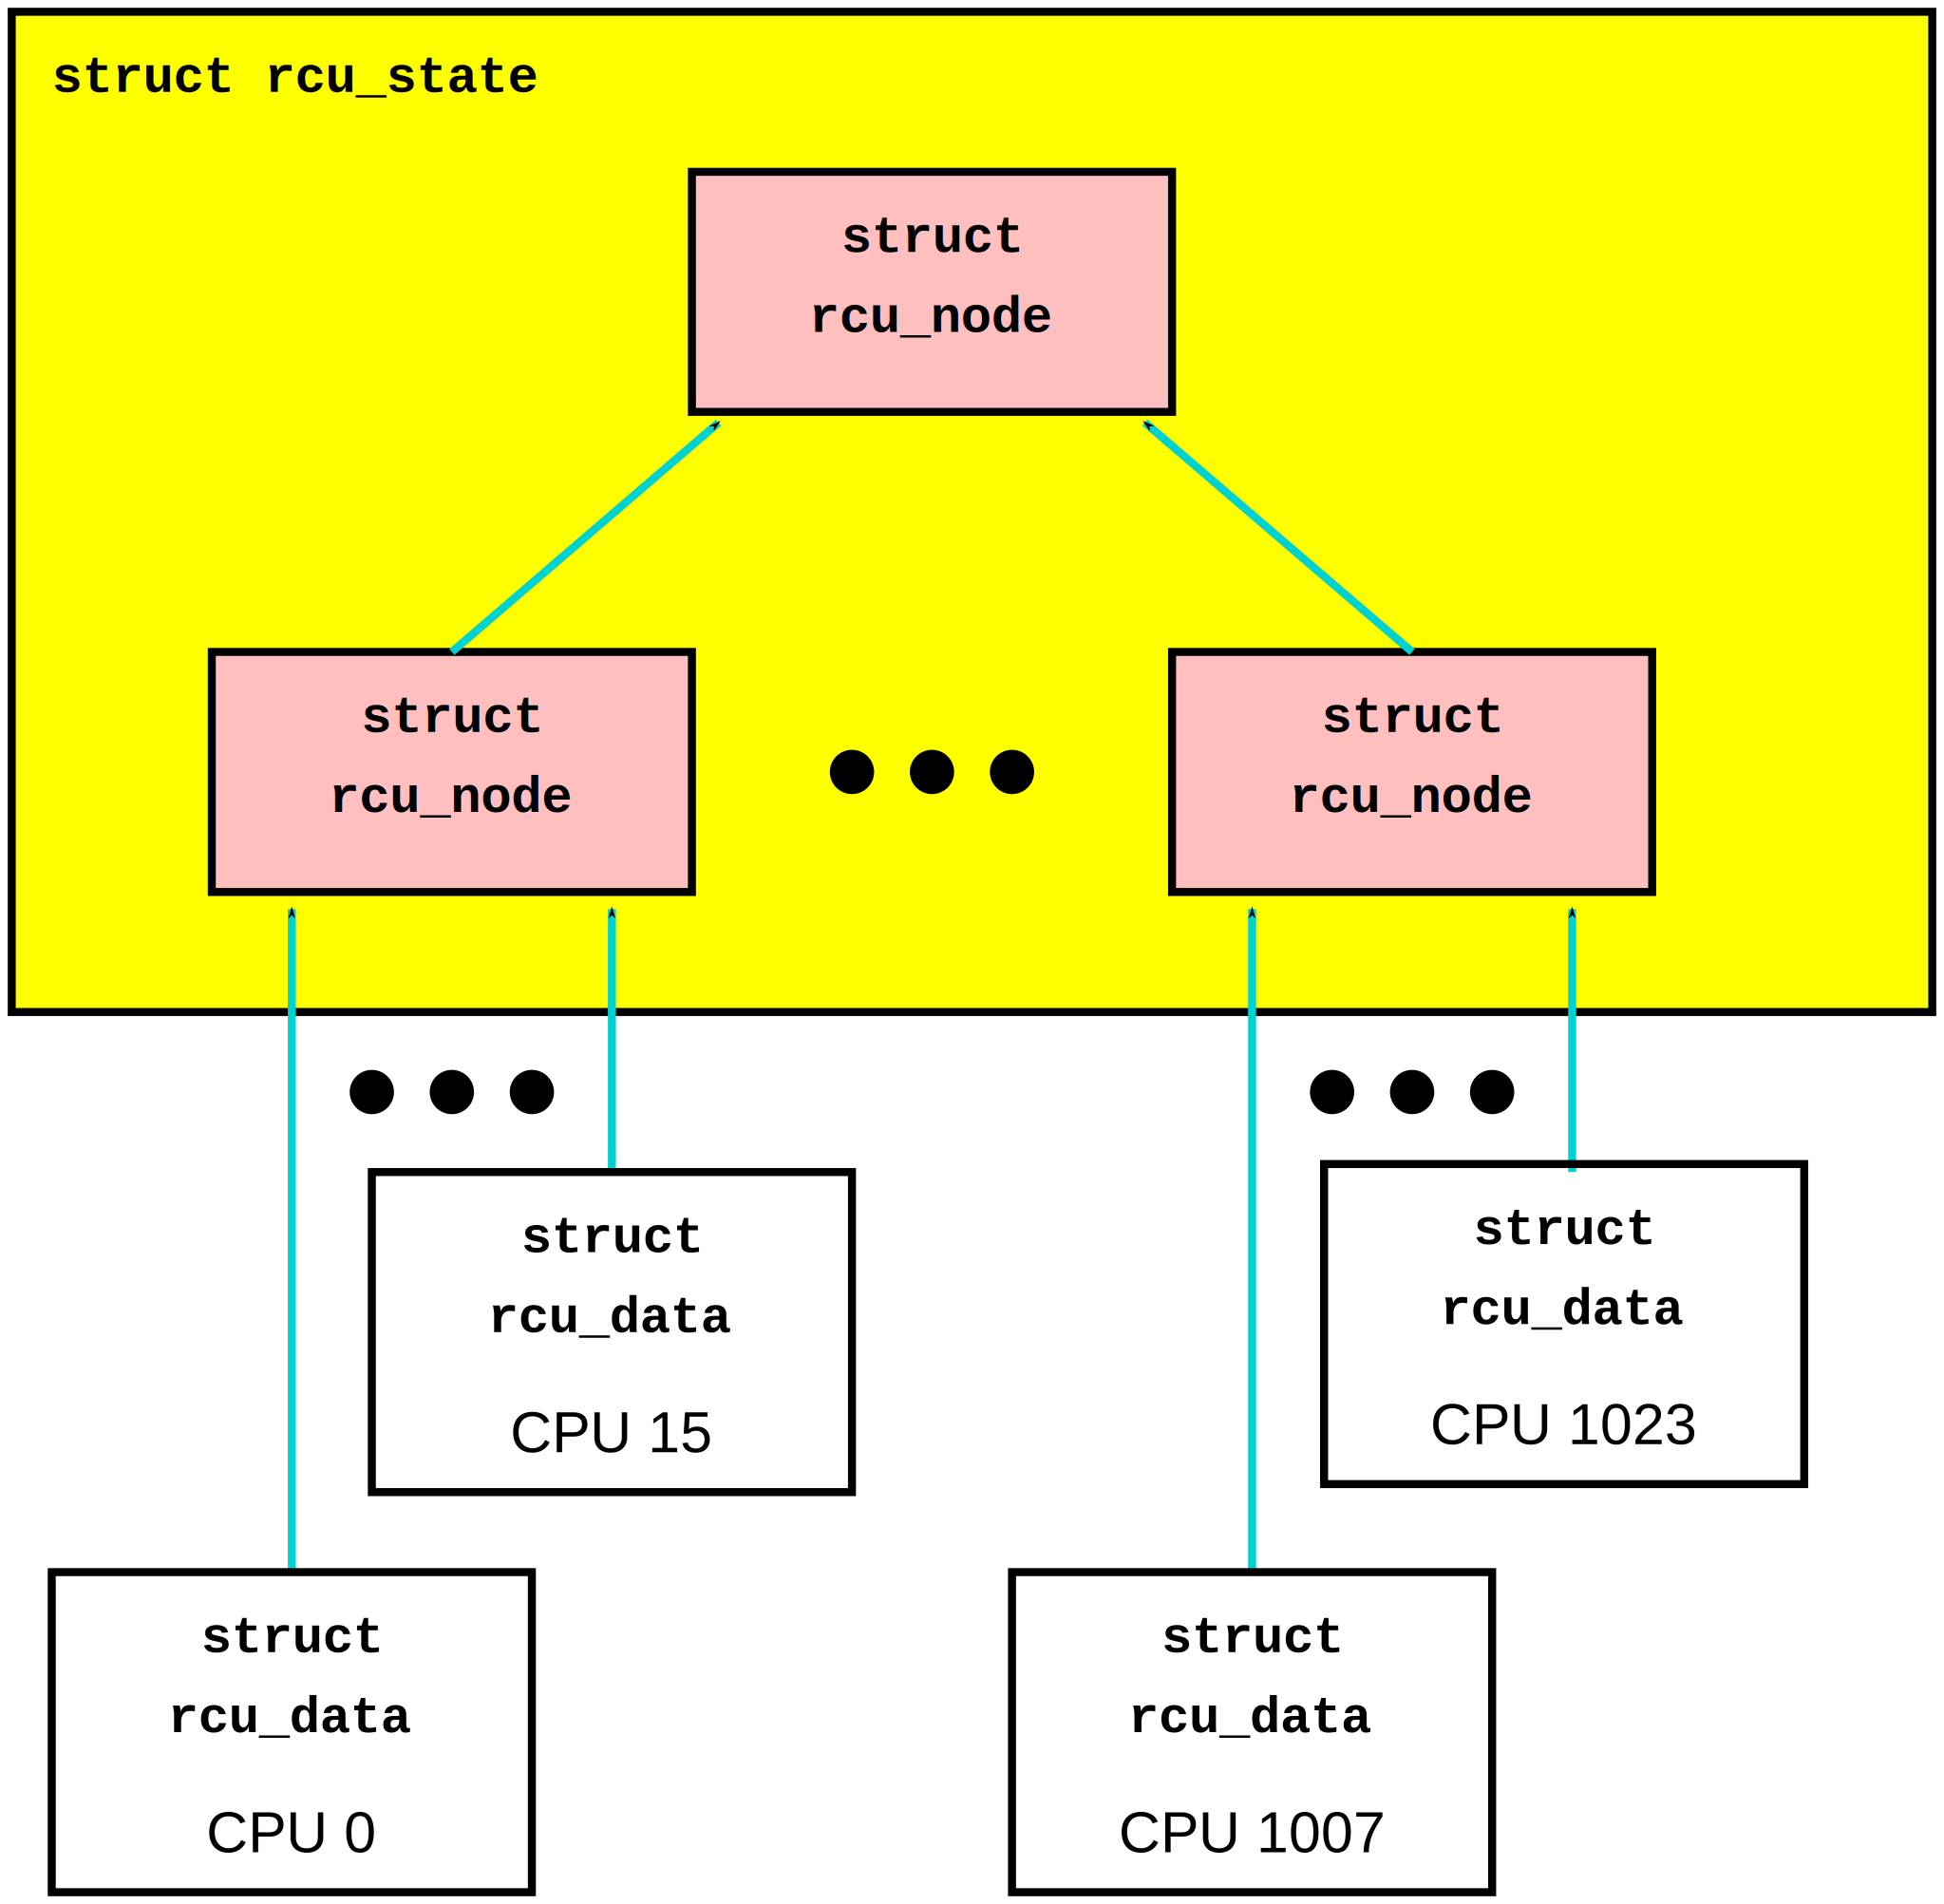
\includegraphics{rcu/design/BigTreeClassicRCU}}
\end{center}

This diagram shows an enclosing \co{rcu_state} structure containing a tree
of \co{rcu_node} structures.
Each leaf node of the \co{rcu_node} tree has up
to 16 \co{rcu_data} structures associated with it, so that there are
\co{NR_CPUS} number of \co{rcu_data} structures, one for each possible CPU\@.
This structure is adjusted at boot time, if needed, to handle the common
case where \co{nr_cpu_ids} is much less than \co{NR_CPUs}.
For example, a number of Linux distributions set \co{NR_CPUs=4096},
which results in a three-level \co{rcu_node} tree.
If the actual hardware has only 16 CPUs, RCU will adjust itself
at boot time, resulting in an \co{rcu_node} tree with only a single node.

The purpose of this combining tree is to allow per-CPU events
such as quiescent states, dyntick-idle transitions,
and CPU hotplug operations to be processed efficiently
and scalably.
Quiescent states are recorded by the per-CPU \co{rcu_data} structures,
and other events are recorded by the leaf-level \co{rcu_node}
structures.
All of these events are combined at each level of the tree until finally
grace periods are completed at the tree's root \co{rcu_node}
structure.
A grace period can be completed at the root once every CPU
(or, in the case of \co{CONFIG_PREEMPT_RCU}, task)
has passed through a quiescent state.
Once a grace period has completed, record of that fact is propagated
back down the tree.

As can be seen from the diagram, on a 64-bit system
a two-level tree with 64 leaves can accommodate 1,024 CPUs, with a fanout
of 64 at the root and a fanout of 16 at the leaves.

\QuickQuiz{
  Why isn't the fanout at the leaves also 64?
}\QuickQuizAnswer{
  Because there are more types of events that affect the leaf-level
  \co{rcu_node} structures than further up the tree.
  Therefore, if the
  leaf \co{rcu_node} structures have fanout of 64, the contention on
  these structures' \co{->structures} becomes excessive.
  Experimentation
  on a wide variety of systems has shown that a fanout of 16 works well
  for the leaves of the \co{rcu_node} tree.

  Of course, further experience with systems having hundreds or
  thousands of CPUs may demonstrate that the fanout for the non-leaf
  \co{rcu_node} structures must also be reduced.
  Such reduction can be
  easily carried out when and if it proves necessary.
  In the meantime,
  if you are using such a system and running into contention problems
  on the non-leaf \co{rcu_node} structures, you may use the
  \co{CONFIG_RCU_FANOUT} kernel configuration parameter to reduce the
  non-leaf fanout as needed.

  Kernels built for systems with strong NUMA characteristics might
  also need to adjust \co{CONFIG_RCU_FANOUT} so that the domains of
  the \co{rcu_node} structures align with hardware boundaries.
  However, there has thus far been no need for this.
}\QuickQuizEnd

If your system has more than 1,024 CPUs (or more than 512 CPUs on a
32-bit system), then RCU will automatically add more levels to the tree.
For example, if you are crazy enough to build a 64-bit system with
65,536 CPUs, RCU would configure the \co{rcu_node} tree as follows:

\begin{center}
\resizebox{\columnwidth}{!}{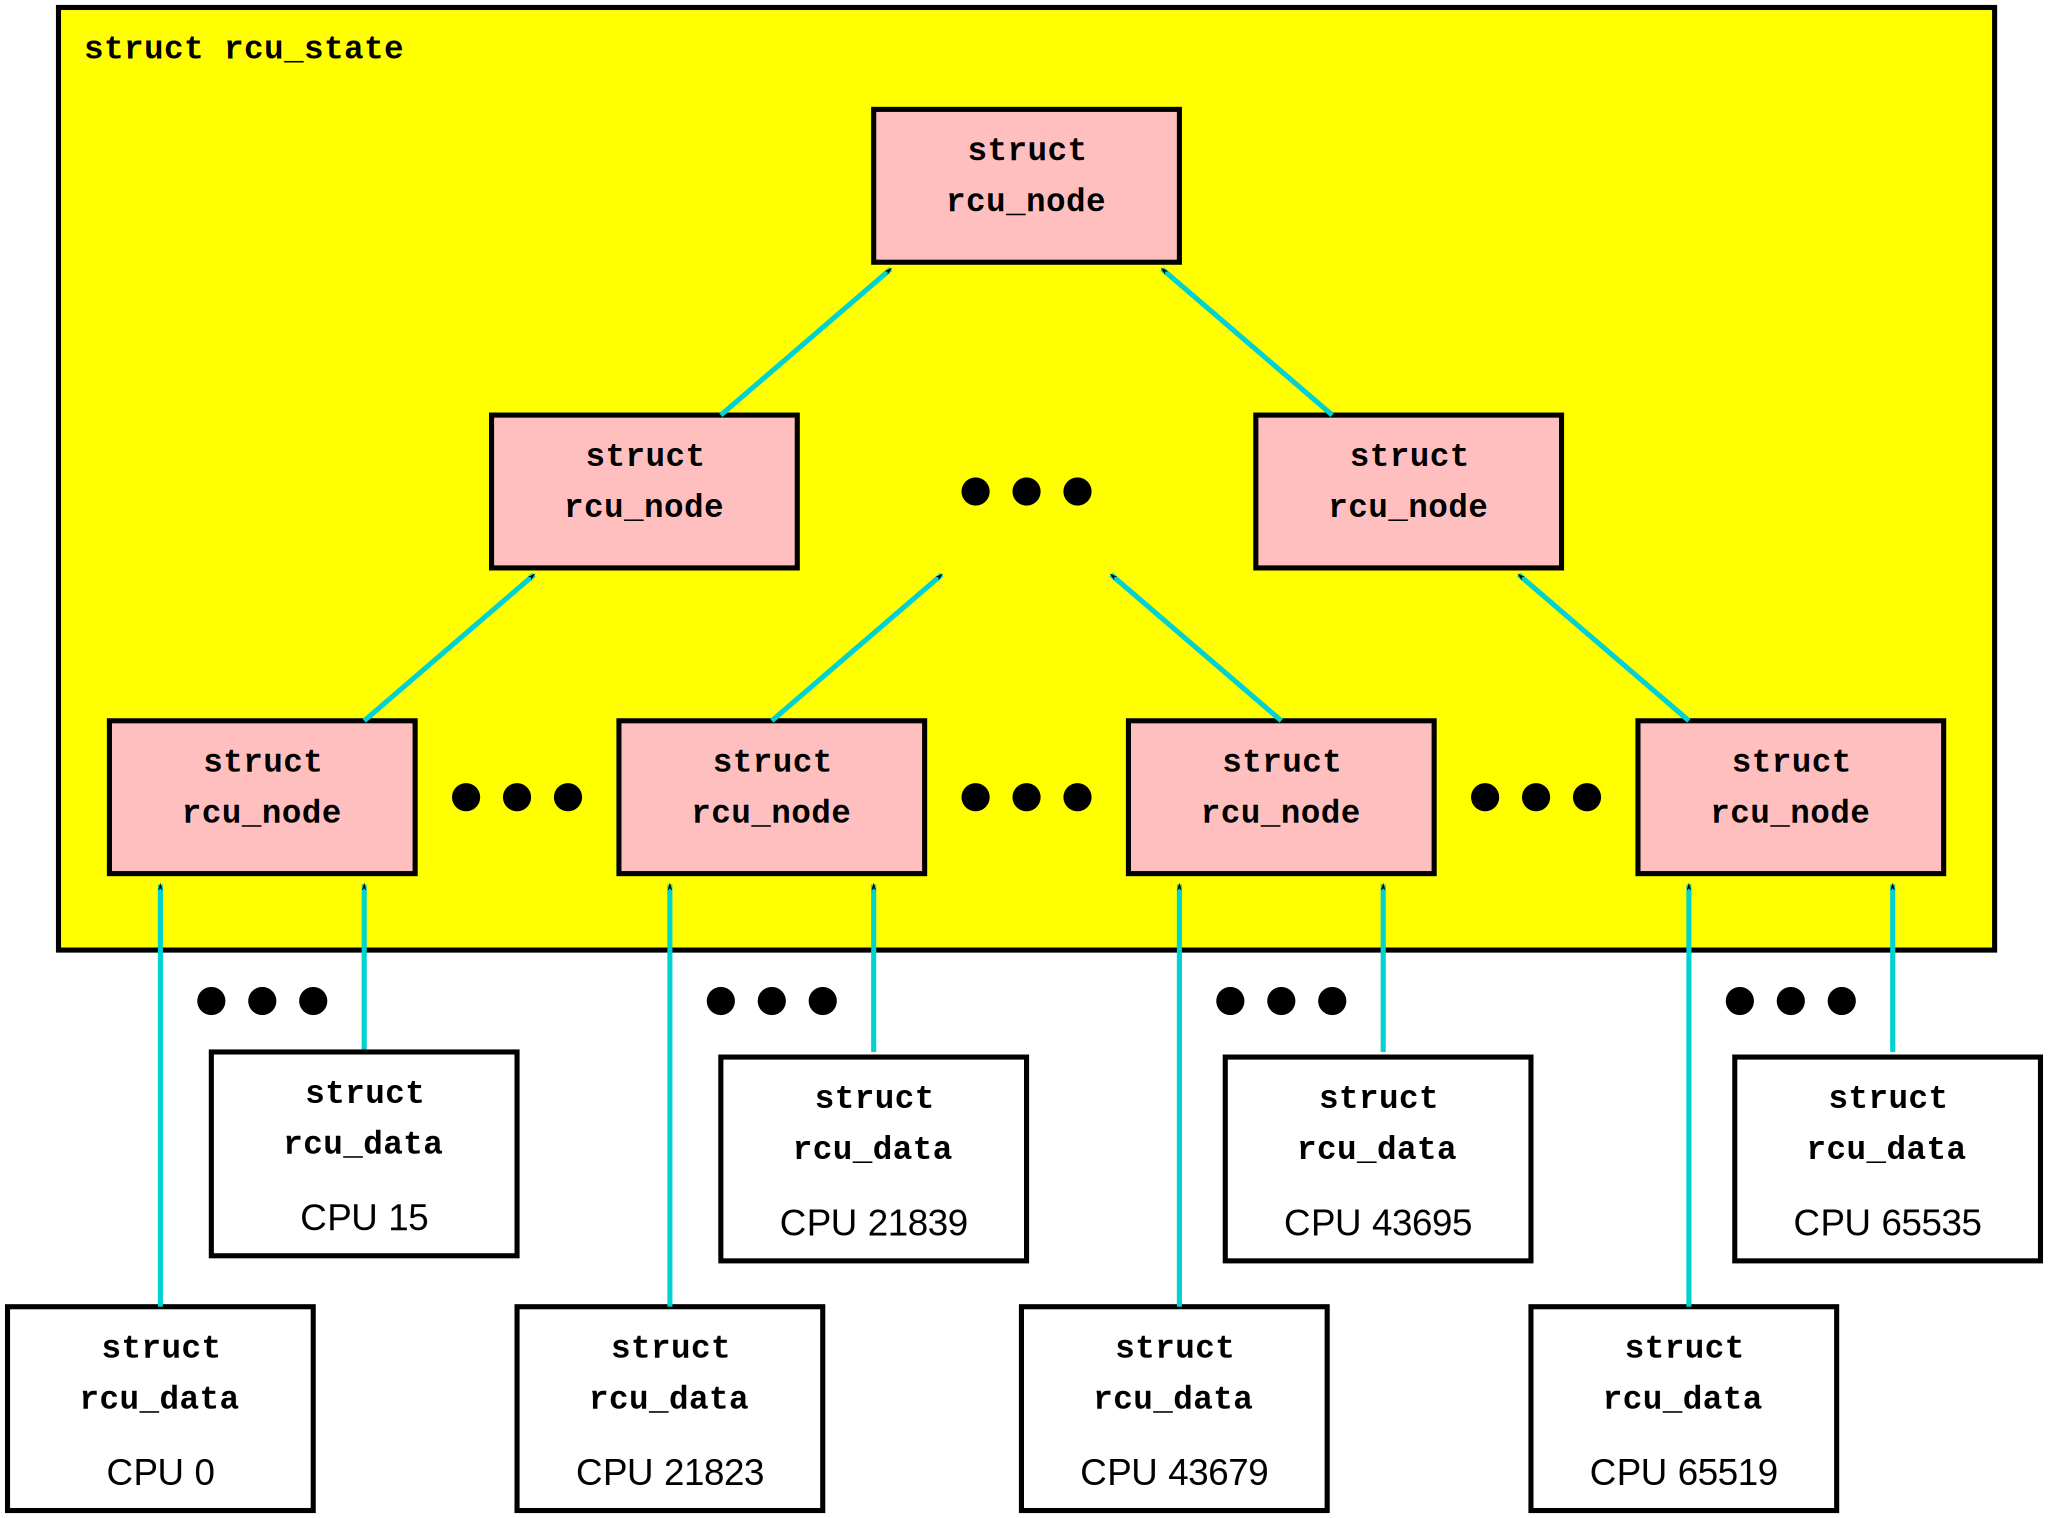
\includegraphics{rcu/design/HugeTreeClassicRCU}}
\end{center}

RCU currently permits up to a four-level tree, which on a 64-bit system
accommodates up to 4,194,304 CPUs, though only a mere 524,288 CPUs for
32-bit systems.
On the other hand, you can set both
\co{CONFIG_RCU_FANOUT} and \co{CONFIG_RCU_FANOUT_LEAF} to be as small as~2,
which would result in a 16-CPU test using a 4-level tree.
This can be
useful for testing large-system capabilities on small test machines.

This multi-level combining tree allows us to get most of the performance
and scalability benefits of partitioning, even though RCU grace-period
detection is inherently a global operation.
The trick here is that only
the last CPU to report a quiescent state into a given \co{rcu_node}
structure need advance to the \co{rcu_node} structure at the next level
up the tree.
This means that at the leaf-level \co{rcu_node} structure,
only one access out of sixteen will progress up the tree.
For the
internal \co{rcu_node} structures, the situation is even more extreme:
Only one access out of sixty-four will progress up the tree.
Because the
vast majority of the CPUs do not progress up the tree, the lock
contention remains roughly constant up the tree.
No matter how many CPUs
there are in the system, at most 64 quiescent-state reports per grace
period will progress all the way to the root \co{rcu_node} structure,
thus ensuring that the lock contention on that root \co{rcu_node}
structure remains acceptably low.

In effect, the combining tree acts like a big shock absorber, keeping
lock contention under control at all tree levels regardless of the level
of loading on the system.

RCU updaters wait for normal grace periods by registering RCU callbacks,
either directly via \co{call_rcu()} or indirectly via
\co{synchronize_rcu()} and friends.
RCU callbacks are represented by
\co{rcu_head} structures, which are queued on \co{rcu_data} structures
while they are waiting for a grace period to elapse, as shown in the
following figure:

\begin{center}
\resizebox{.8\columnwidth}{!}{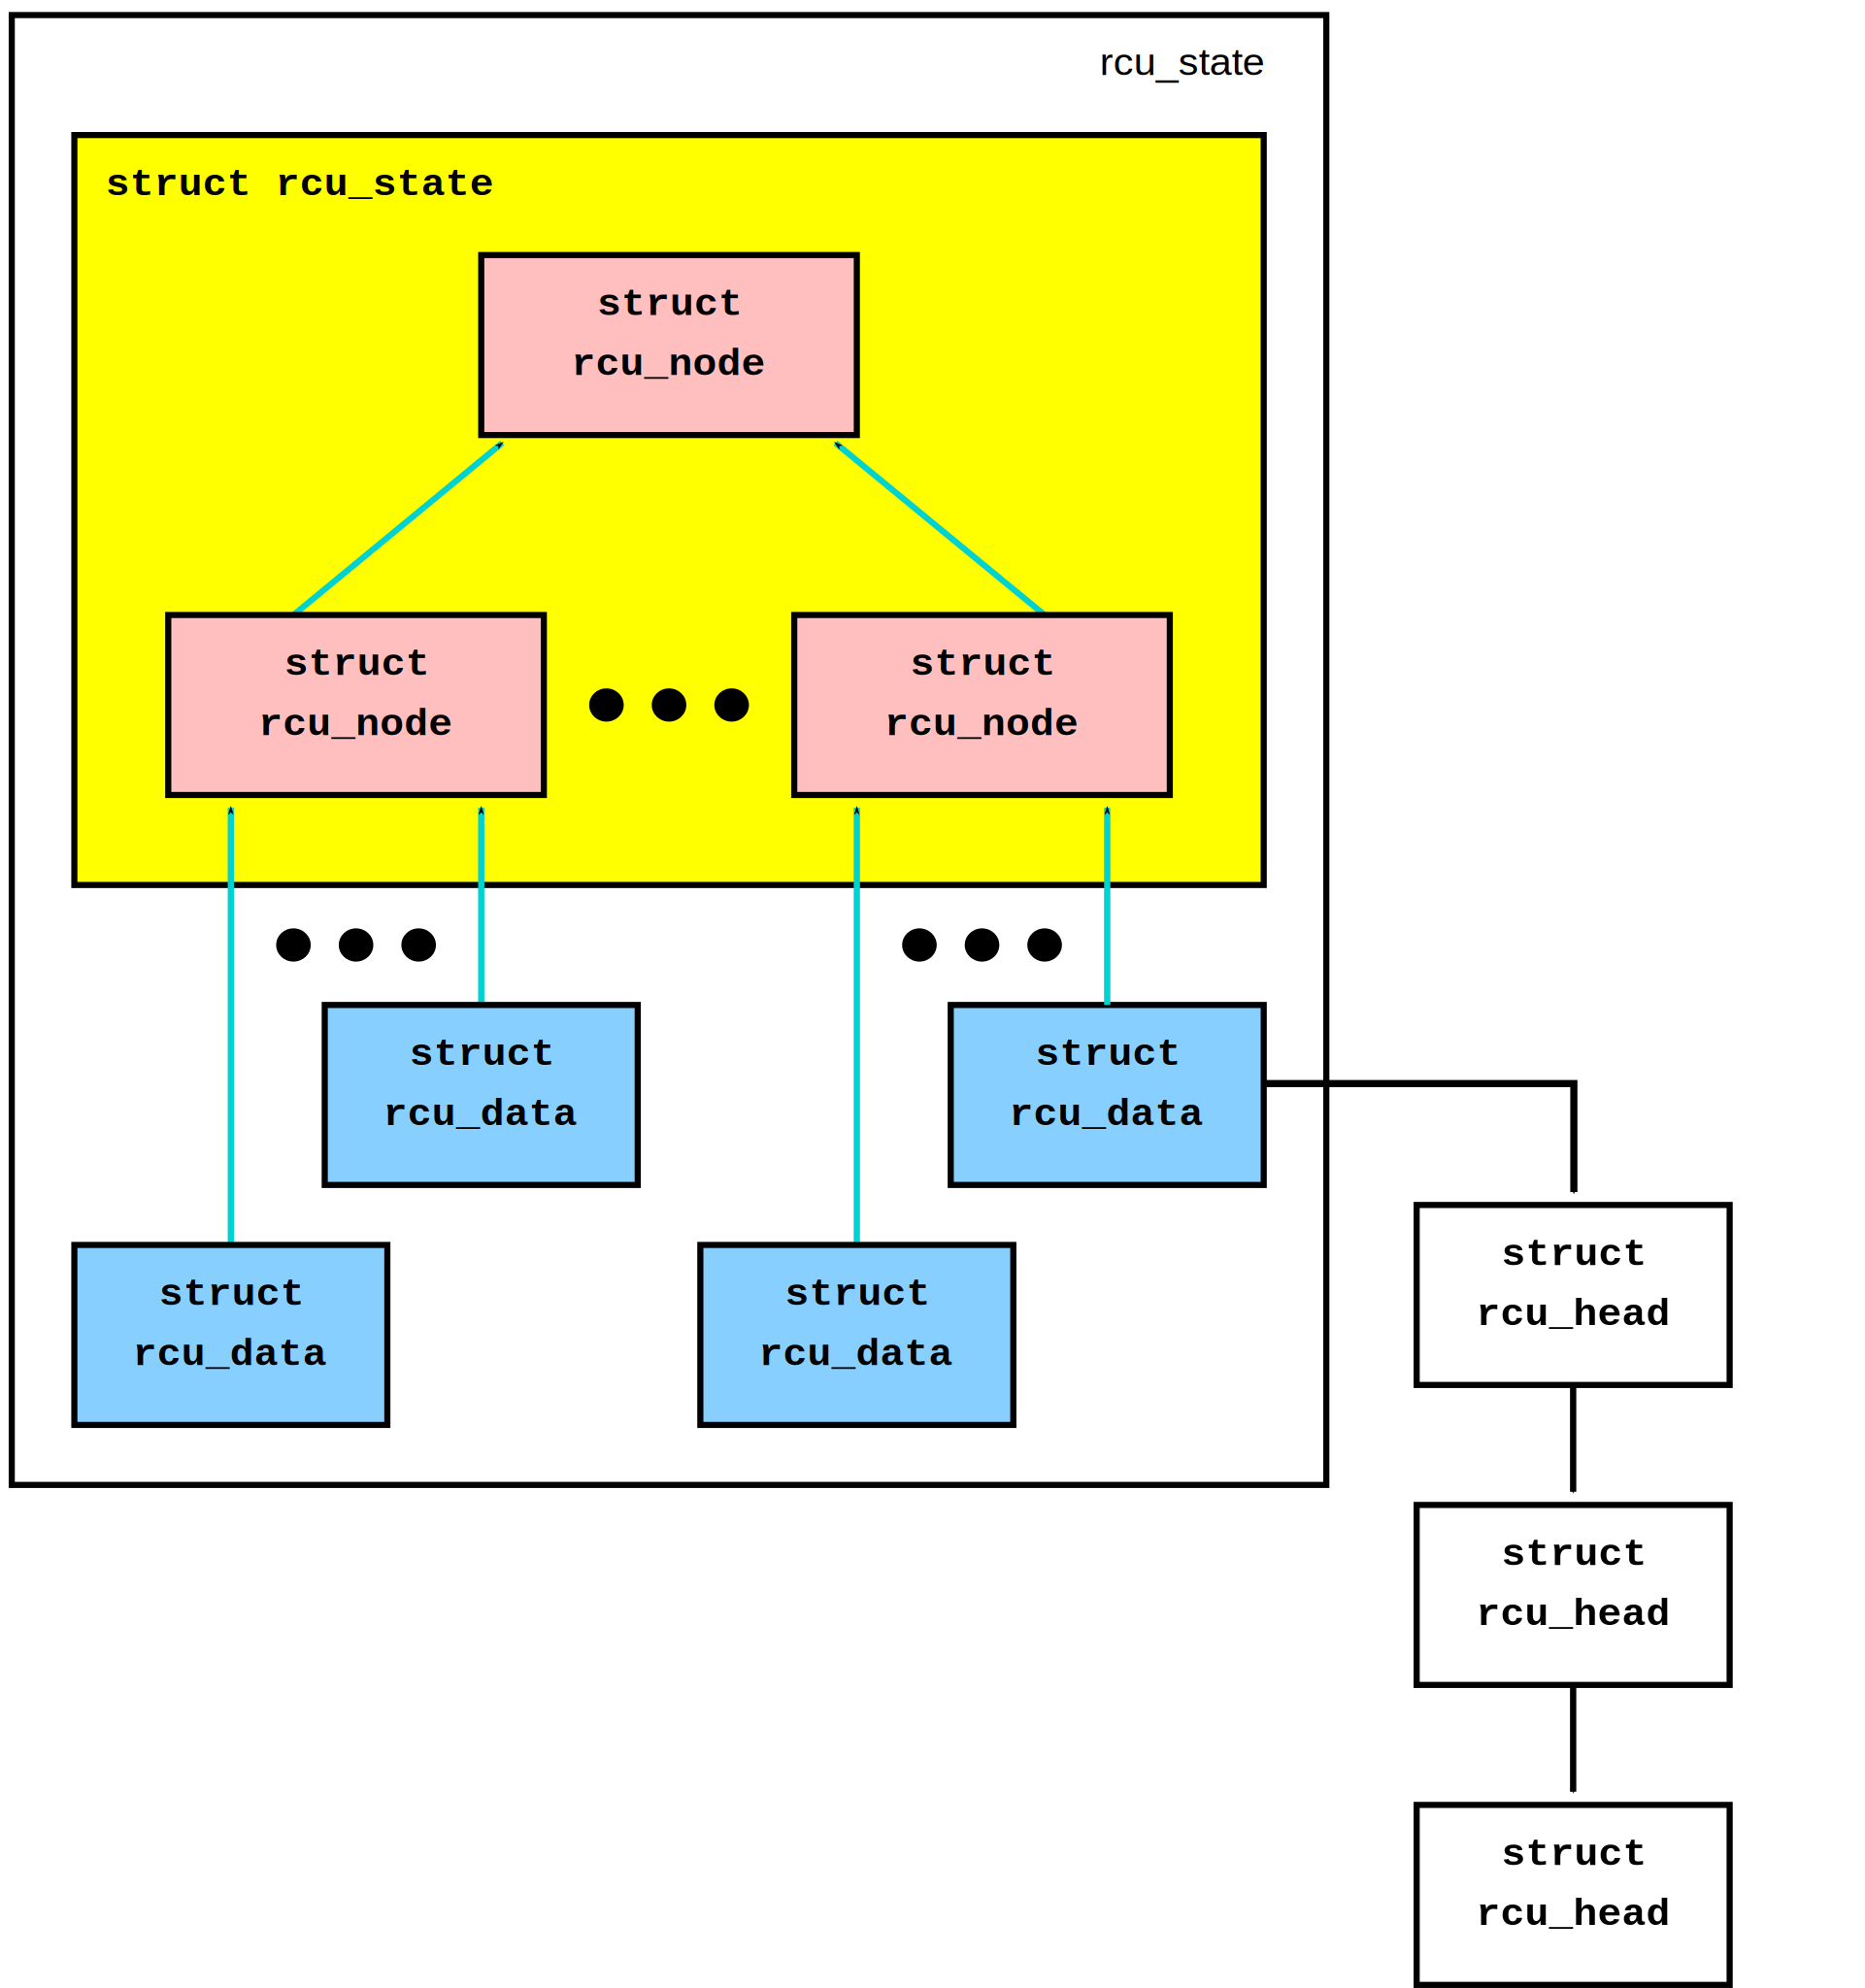
\includegraphics{rcu/design/BigTreePreemptRCUBHdyntickCB}}
\end{center}

This figure shows how \co{TREE_RCU}'s and \co{PREEMPT_RCU}'s major data
structures are related.
Lesser data structures will be introduced with
the algorithms that make use of them.

Note that each of the data structures in the above figure has its own
synchronization:

\begin{enumerate}
\item Each \co{rcu_state} structures has a lock and a mutex, and some fields
   are protected by the corresponding root \co{rcu_node} structure's lock.
\item Each \co{rcu_node} structure has a spinlock.
\item The fields in \co{rcu_data} are private to the corresponding CPU,
   although a few can be read and written by other CPUs.
\end{enumerate}

It is important to note that different data structures can have very
different ideas about the state of RCU at any given time.
For but one
example, awareness of the start or end of a given RCU grace period
propagates slowly through the data structures.
This slow propagation is
absolutely necessary for RCU to have good read-side performance.
If this
balkanized implementation seems foreign to you, one useful trick is to
consider each instance of these data structures to be a different
person, each having the usual slightly different view of reality.

The general role of each of these data structures is as follows:

\begin{description}
\item[\tco{rcu_state}:]
   This structure forms the interconnection between the
   \co{rcu_node} and \co{rcu_data} structures, tracks grace periods,
   serves as short-term repository for callbacks orphaned by CPU-hotplug
   events, maintains \co{rcu_barrier()} state, tracks expedited
   grace-period state, and maintains state used to force quiescent
   states when grace periods extend too long,
\item[\tco{rcu_node}:]
   This structure forms the combining tree that propagates
   quiescent-state information from the leaves to the root, and also
   propagates grace-period information from the root to the leaves.
   It
   provides local copies of the grace-period state in order to allow
   this information to be accessed in a synchronized manner without
   suffering the scalability limitations that would otherwise be imposed
   by global locking.
   In \co{CONFIG_PREEMPT_RCU} kernels, it manages the
   lists of tasks that have blocked while in their current RCU read-side
   critical section.
   In \co{CONFIG_PREEMPT_RCU} with
   \co{CONFIG_RCU_BOOST}, it manages the per-\co{rcu_node}
   priority-boosting kernel threads (kthreads) and state.
   Finally, it
   records CPU-hotplug state in order to determine which CPUs should be
   ignored during a given grace period.
\item[\tco{rcu_data}:]
   This per-CPU structure is the focus of quiescent-state
   detection and RCU callback queuing.
   It also tracks its relationship
   to the corresponding leaf \co{rcu_node} structure to allow
   more-efficient propagation of quiescent states up the \co{rcu_node}
   combining tree.
   Like the \co{rcu_node} structure, it provides a local
   copy of the grace-period information to allow for-free synchronized
   access to this information from the corresponding CPU\@.
   Finally, this
   structure records past dyntick-idle state for the corresponding CPU
   and also tracks statistics.
\item[\tco{rcu_head}:] This structure represents RCU callbacks, and is the
   only structure allocated and managed by RCU users.
   The \co{rcu_head}
   structure is normally embedded within the RCU-protected data
   structure.
\end{description}

If all you wanted from this article was a general notion of how RCU's
data structures are related, you are done.
Otherwise, each of the
following sections give more details on the \co{rcu_state}, \co{rcu_node}
and \co{rcu_data} data structures.

\subsubsection{The \texttt{rcu\_state} Structure}

The \co{rcu_state} structure is the base structure that represents the
state of RCU in the system.
This structure forms the interconnection
between the \co{rcu_node} and \co{rcu_data} structures, tracks grace
periods, contains the lock used to synchronize with CPU-hotplug events,
and maintains state used to force quiescent states when grace periods
extend too long.

A few of the \co{rcu_state} structure's fields are discussed, singly and
in groups, in the following sections. The more specialized fields are
covered in the discussion of their use.

\paragraph{Relationship to \texttt{rcu\_node} and \texttt{rcu\_data} Structures}

This portion of the \co{rcu_state} structure is declared as follows:

\begin{VerbatimN}
		struct rcu_node node[NUM_RCU_NODES];
		struct rcu_node *level[NUM_RCU_LVLS + 1];
		struct rcu_data __percpu *rda;
\end{VerbatimN}

\QuickQuiz{
  Wait a minute!
  You said that the \co{rcu_node} structures formed a
  tree, but they are declared as a flat array!
  What gives?
}\QuickQuizAnswer{
  The tree is laid out in the array.
  The first node In the array is the
  head, the next set of nodes in the array are children of the head
  node, and so on until the last set of nodes in the array are the
  leaves.
  See the diagrams following this Quick Quiz to see how this works.
}\QuickQuizEnd

The \co{rcu_node} tree is embedded into the \co{->node[]} array as shown
in the following figure:

\begin{center}
\resizebox{.8\columnwidth}{!}{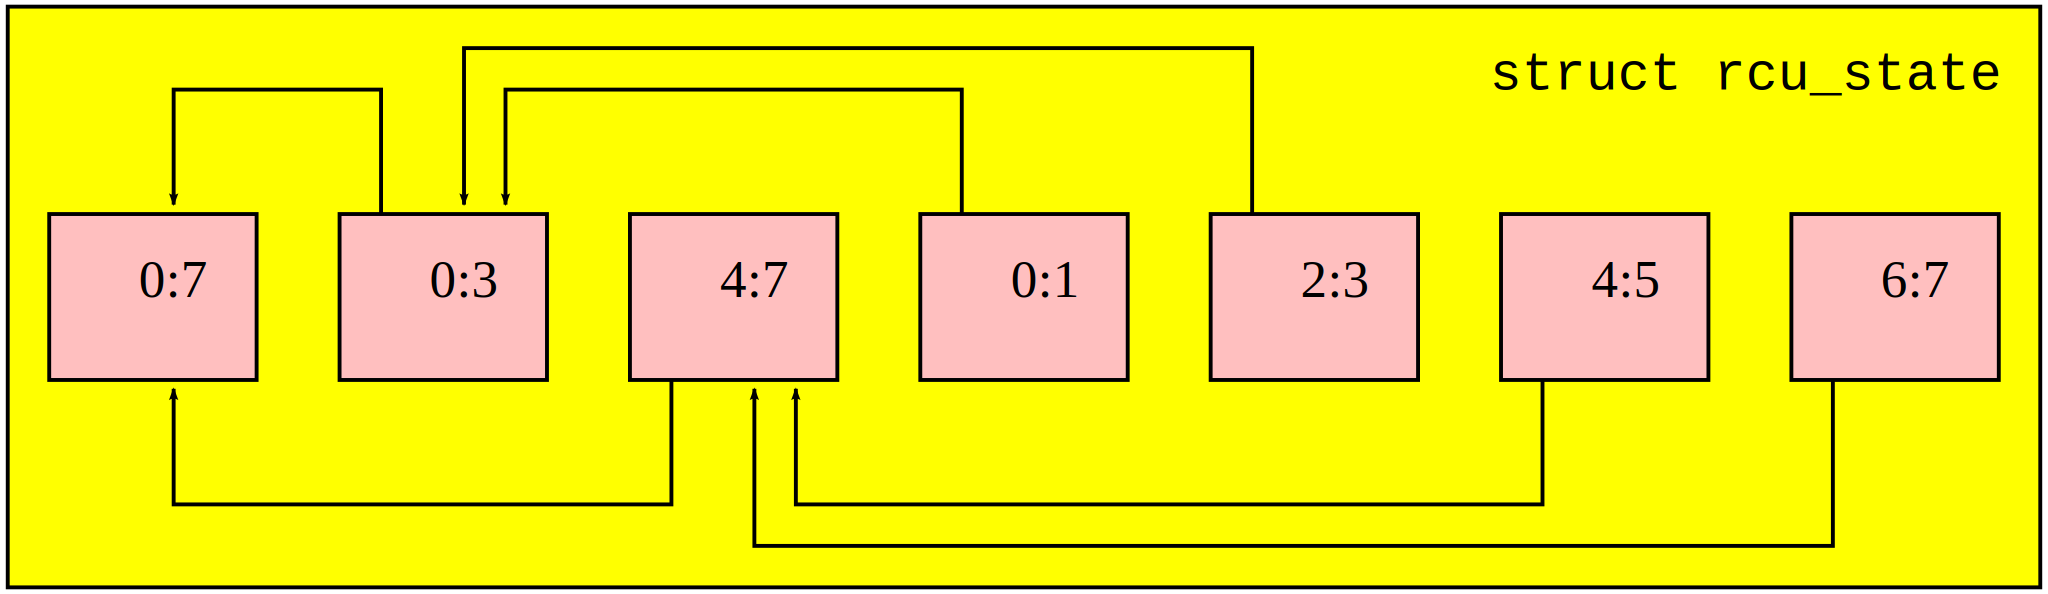
\includegraphics{rcu/design/TreeMapping}}
\end{center}

One interesting consequence of this mapping is that a breadth-first
traversal of the tree is implemented as a simple linear scan of the
array, which is in fact what the \co{rcu_for_each_node_breadth_first()}
macro does.
This macro is used at the beginning and ends of grace
periods.

Each entry of the \co{->level} array references the first \co{rcu_node}
structure on the corresponding level of the tree, for example, as shown
below:

\begin{center}
\resizebox{.8\columnwidth}{!}{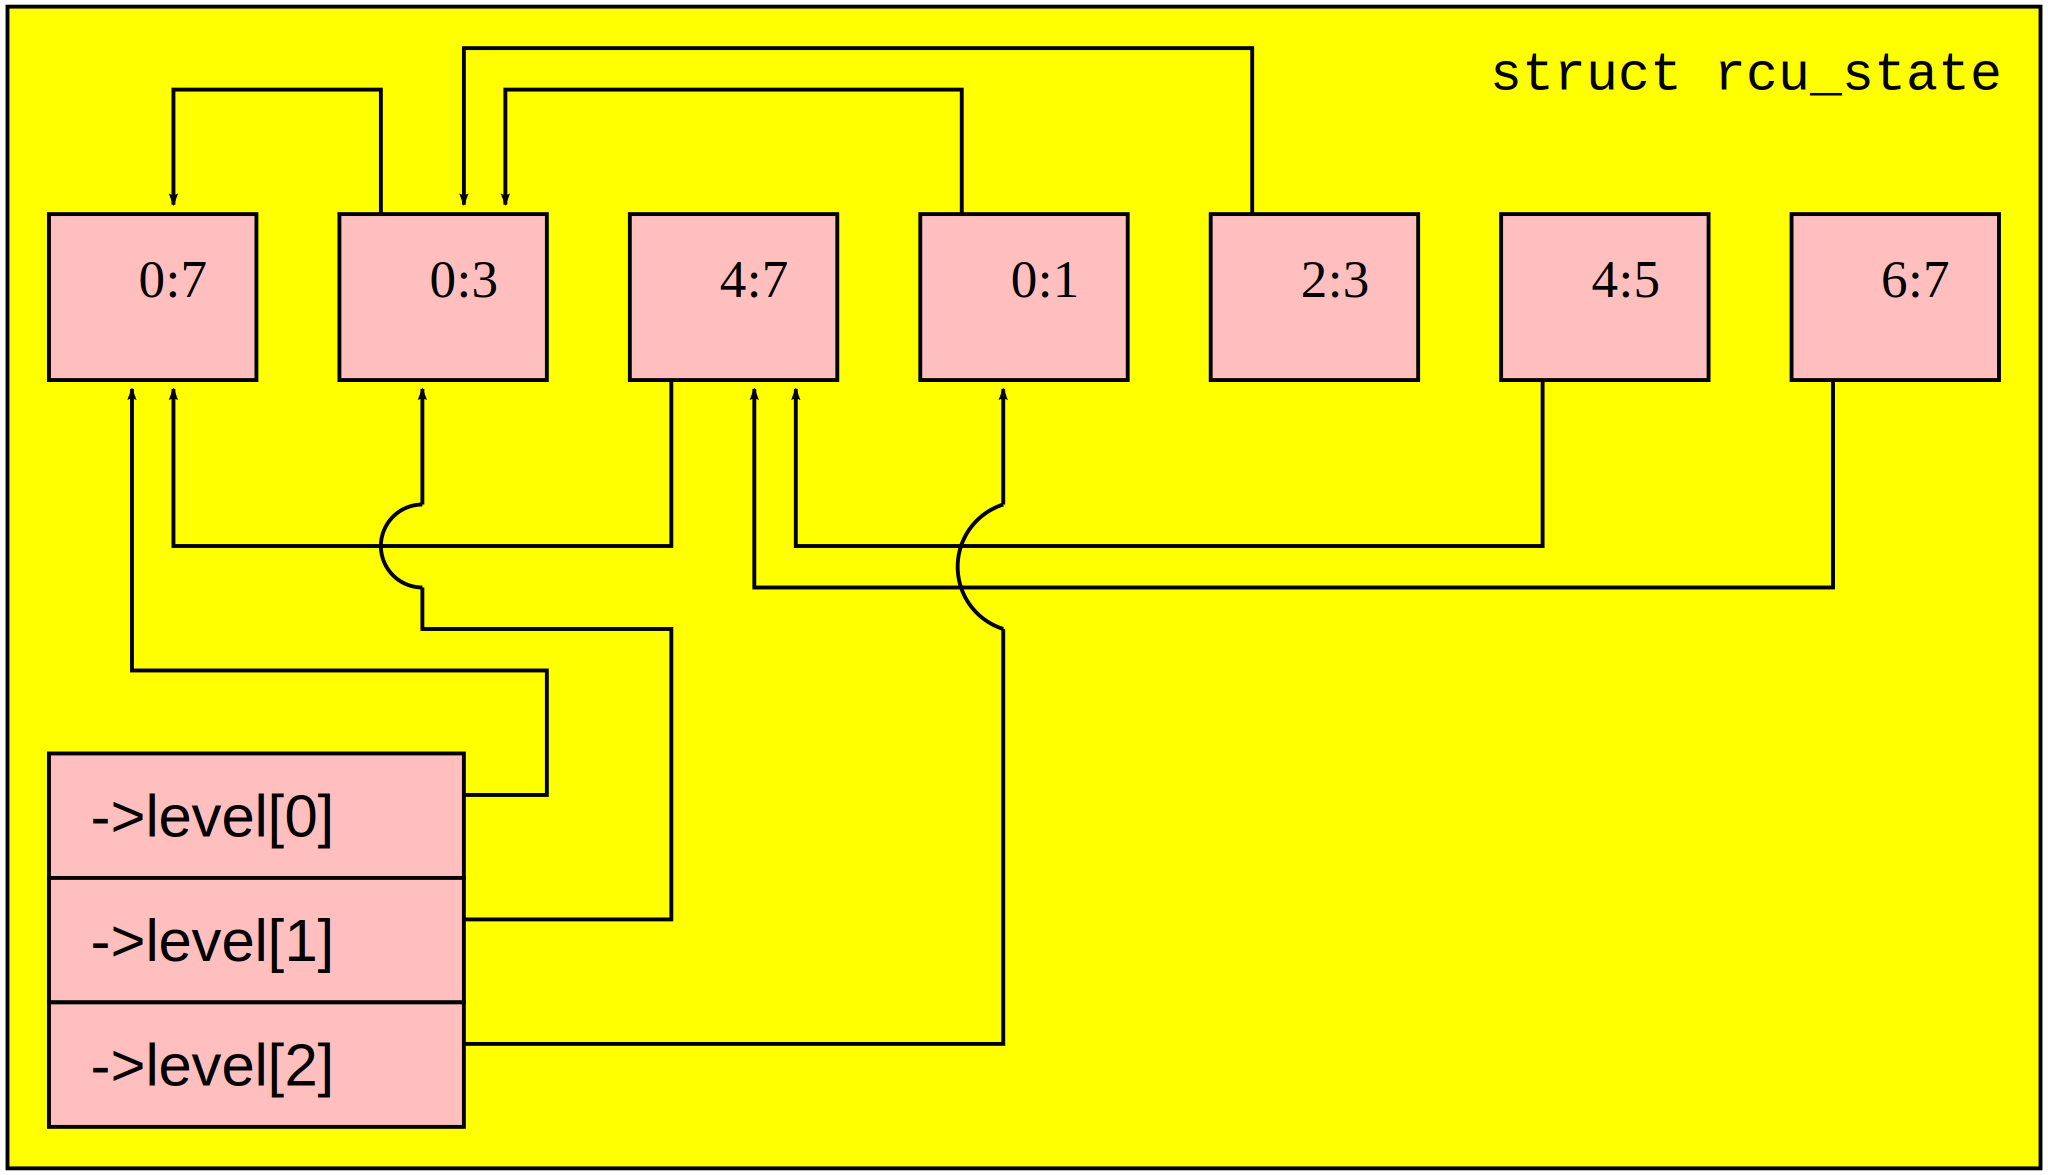
\includegraphics{rcu/design/TreeMappingLevel}}
\end{center}

The zero\textsuperscript{th} element of the array references the root
\co{rcu_node} structure, the first element references the first child of
the root \co{rcu_node}, and finally the second element references the
first leaf \co{rcu_node} structure.

For whatever it is worth, if you draw the tree to be tree-shaped rather
than array-shaped, it is easy to draw a planar representation:

\begin{center}
\resizebox{\columnwidth}{!}{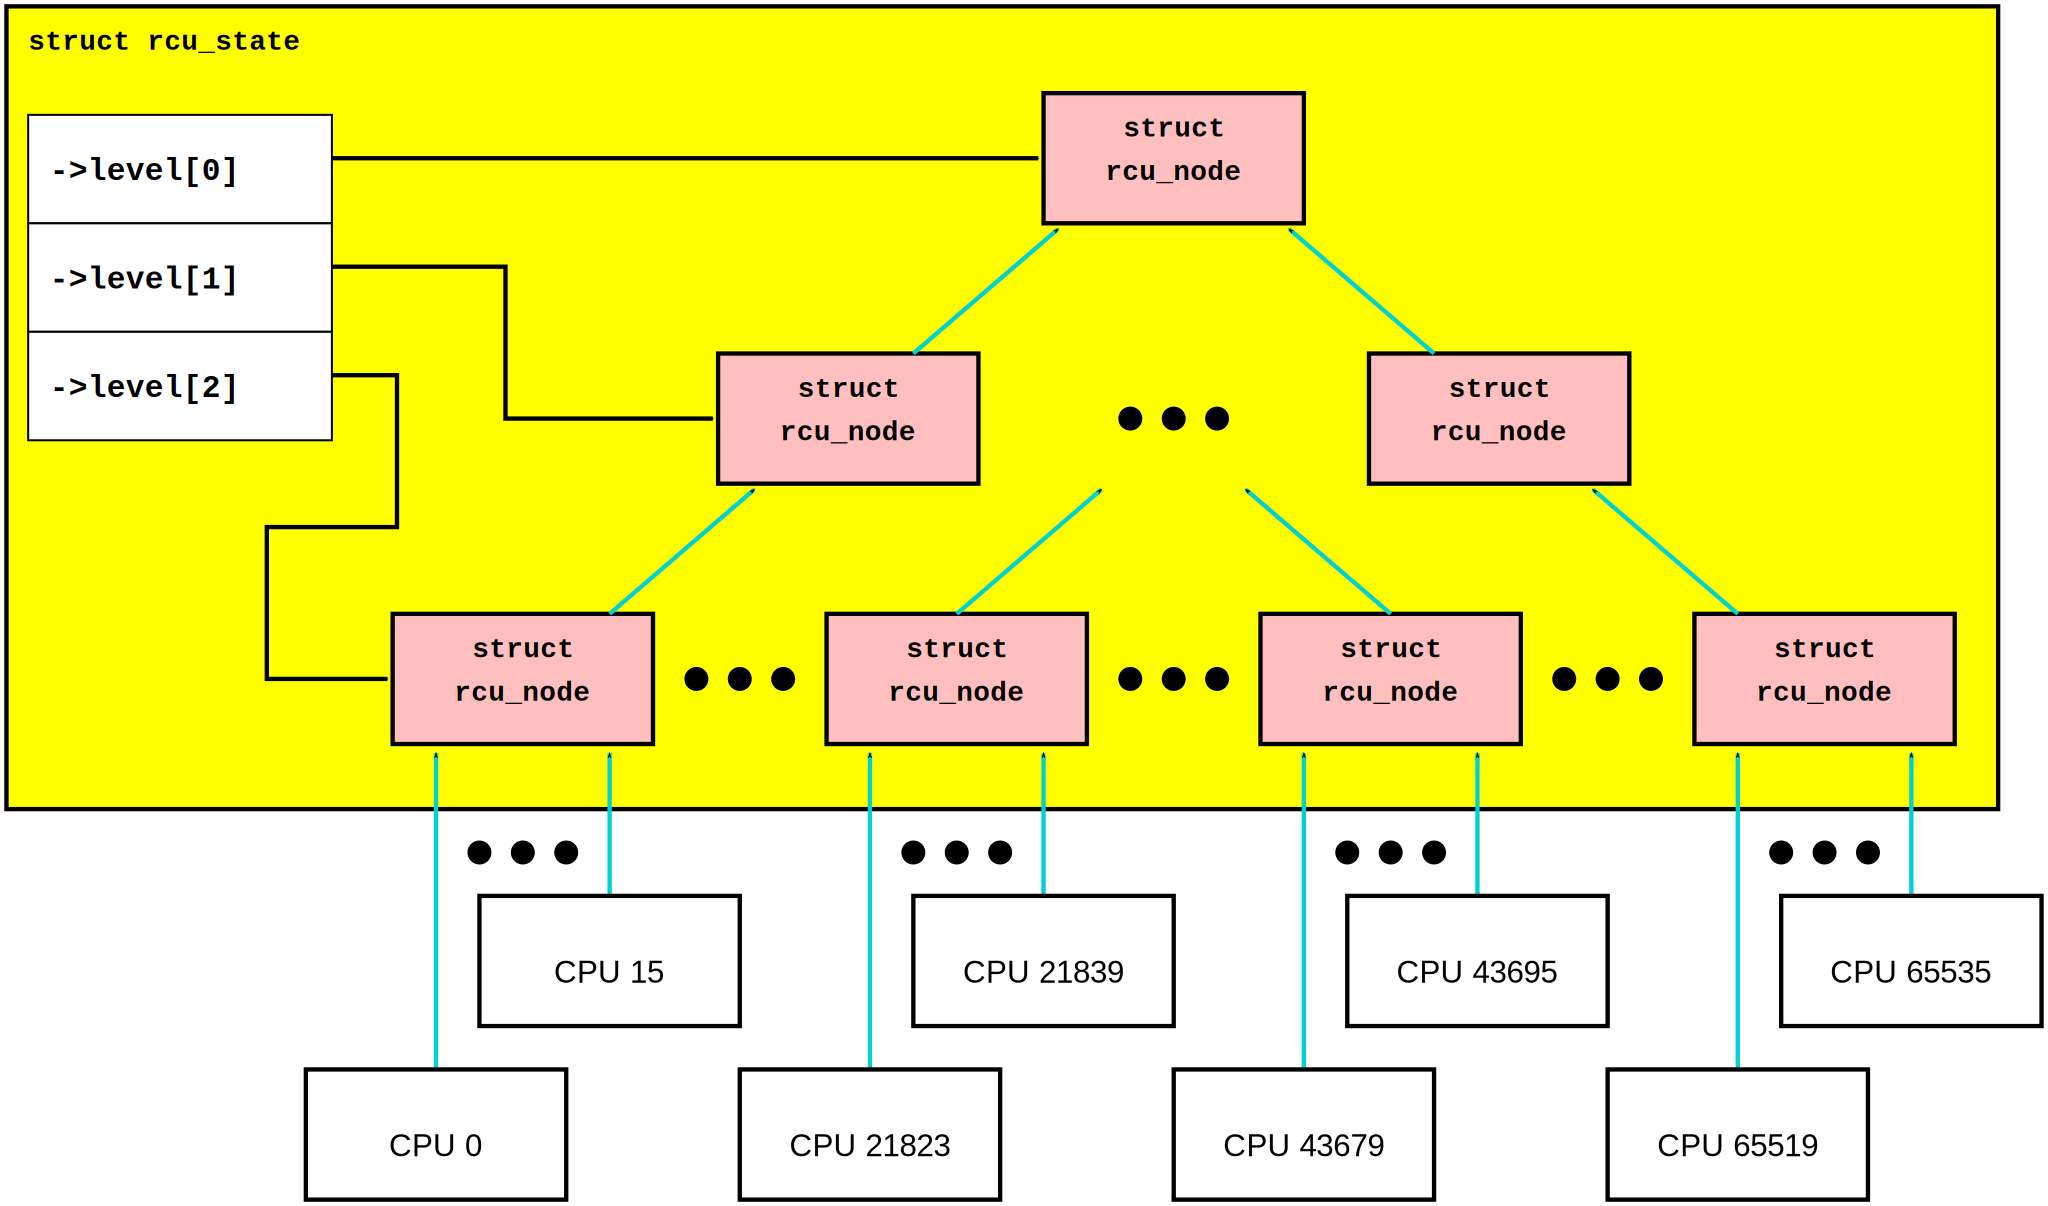
\includegraphics{rcu/design/TreeLevel}}
\end{center}

Finally, the \co{->rda} field references a per-CPU pointer to the
corresponding CPU's \co{rcu_data} structure.

All of these fields are constant once initialization is complete, and
therefore need no protection.

\paragraph{Grace-Period Tracking}

This portion of the \co{rcu_state} structure is declared as follows:

\begin{VerbatimN}
	unsigned long gp_seq;
\end{VerbatimN}

RCU grace periods are numbered, and the \co{->gp_seq} field contains the
current grace-period sequence number.
The bottom two bits are the state
of the current grace period, which can be zero for not yet started or
one for in progress. In other words, if the bottom two bits of
\co{->gp_seq} are zero, then RCU is idle. Any other value in the bottom
two bits indicates that something is broken.
This field is protected by
the root \co{rcu_node} structure's \co{->lock} field.

There are \co{->gp_seq} fields in the \co{rcu_node} and \co{rcu_data}
structures as well.
The fields in the \co{rcu_state} structure represent
the most current value, and those of the other structures are compared
in order to detect the beginnings and ends of grace periods in a
distributed fashion.
The values flow from \co{rcu_state} to \co{rcu_node}
(down the tree from the root to the leaves) to \co{rcu_data}.

\paragraph{Miscellaneous}

This portion of the \co{rcu_state} structure is declared as follows:

\begin{VerbatimN}
	unsigned long gp_max;
	char abbr;
	char *name;
\end{VerbatimN}

The \co{->gp_max} field tracks the duration of the longest grace period
in jiffies.
It is protected by the root \co{rcu_node}'s \co{->lock}.

The \co{->name} and \co{->abbr} fields distinguish between preemptible RCU
(\co{rcu_preempt} and \qco{p}) and non-preemptible RCU (\co{rcu_sched} and \qco{s}).
These fields are used for diagnostic and tracing purposes.

\subsubsection{The \texttt{rcu\_node} Structure}

The \co{rcu_node} structures form the combining tree that propagates
quiescent-state information from the leaves to the root and also that
propagates grace-period information from the root down to the leaves.
They provide local copies of the grace-period state in order to allow
this information to be accessed in a synchronized manner without
suffering the scalability limitations that would otherwise be imposed by
global locking.
In \co{CONFIG_PREEMPT_RCU} kernels, they manage the lists
of tasks that have blocked while in their current RCU read-side critical
section.
In \co{CONFIG_PREEMPT_RCU} with \co{CONFIG_RCU_BOOST}, they
manage the per-\co{rcu_node} priority-boosting kernel threads
(kthreads) and state.
Finally, they record CPU-hotplug state in order to
determine which CPUs should be ignored during a given grace period.

The \co{rcu_node} structure's fields are discussed, singly and in groups,
in the following sections.

\paragraph{Connection to Combining Tree}

This portion of the \co{rcu_node} structure is declared as follows:

\begin{VerbatimN}
	struct rcu_node *parent;
	u8 level;
	u8 grpnum;
	unsigned long grpmask;
	int grplo;
	int grphi;
\end{VerbatimN}

The \co{->parent} pointer references the \co{rcu_node} one level up in the
tree, and is \co{NULL} for the root \co{rcu_node}.
The RCU implementation
makes heavy use of this field to push quiescent states up the tree.
The
\co{->level} field gives the level in the tree, with the root being at
level zero, its children at level one, and so on.
The \co{->grpnum} field
gives this node's position within the children of its parent, so this
number can range between~0 and~31 on 32-bit systems and between~0 and~63
on 64-bit systems.
The \co{->level} and \co{->grpnum} fields are used only
during initialization and for tracing.
The \co{->grpmask} field is the
bitmask counterpart of \co{->grpnum}, and therefore always has exactly
one bit set.
This mask is used to clear the bit corresponding to this
\co{rcu_node} structure in its parent's bitmasks, which are described
later.
Finally, the \co{->grplo} and \co{->grphi} fields contain the
lowest and highest numbered CPU served by this \co{rcu_node} structure,
respectively.

All of these fields are constant, and thus do not require any
synchronization.

\paragraph{Synchronization}

This field of the \co{rcu_node} structure is declared as follows:

\begin{VerbatimN}
	raw_spinlock_t lock;
\end{VerbatimN}

This field is used to protect the remaining fields in this structure,
unless otherwise stated.
That said, all of the fields in this structure
can be accessed without locking for tracing purposes.
Yes, this can
result in confusing traces, but better some tracing confusion than to be
heisenbugged out of existence.

% .. _grace-period-tracking-1:

\paragraph{Grace-Period Tracking}

This portion of the \co{rcu_node} structure is declared as follows:

\begin{VerbatimN}
	unsigned long gp_seq;
	unsigned long gp_seq_needed;
\end{VerbatimN}

The \co{rcu_node} structures' \co{->gp_seq} fields are the counterparts of
the field of the same name in the \co{rcu_state} structure.
They each may
lag up to one step behind their \co{rcu_state} counterpart.
If the bottom
two bits of a given \co{rcu_node} structure's \co{->gp_seq} field is zero,
then this \co{rcu_node} structure believes that RCU is idle.

The \co{>gp_seq} field of each \co{rcu_node} structure is updated at the
beginning and the end of each grace period.

The \co{->gp_seq_needed} fields record the furthest-in-the-future grace
period request seen by the corresponding \co{rcu_node} structure.
The
request is considered fulfilled when the value of the \co{->gp_seq} field
equals or exceeds that of the \co{->gp_seq_needed} field.

\QuickQuiz{
  Suppose that this \co{rcu_node} structure doesn't see a request for a
  very long time.
  Won't wrapping of the \co{->gp_seq} field cause
  problems?
}\QuickQuizAnswer{
  No, because if the \co{->gp_seq_needed} field lags behind the
  \co{->gp_seq} field, the \co{->gp_seq_needed} field will be updated at
  the end of the grace period.
  Modulo-arithmetic comparisons therefore
  will always get the correct answer, even with wrapping.
}\QuickQuizEnd

\paragraph{Quiescent-State Tracking}

These fields manage the propagation of quiescent states up the combining
tree.

This portion of the \co{rcu_node} structure has fields as follows:

\begin{VerbatimN}
	unsigned long qsmask;
	unsigned long expmask;
	unsigned long qsmaskinit;
	unsigned long expmaskinit;
\end{VerbatimN}

The \co{->qsmask} field tracks which of this \co{rcu_node} structure's
children still need to report quiescent states for the current normal
grace period.
Such children will have a value of~1 in their
corresponding bit.
Note that the leaf \co{rcu_node} structures should be
thought of as having \co{rcu_data} structures as their children.
Similarly, the \co{->expmask} field tracks which of this \co{rcu_node}
structure's children still need to report quiescent states for the
current expedited grace period.
An expedited grace period has the same
conceptual properties as a normal grace period, but the expedited
implementation accepts extreme CPU overhead to obtain much lower
grace-period latency, for example, consuming a few tens of microseconds
worth of CPU time to reduce grace-period duration from milliseconds to
tens of microseconds.
The \co{->qsmaskinit} field tracks which of this
\co{rcu_node} structure's children cover for at least one online CPU\@.
This mask is used to initialize \co{->qsmask}, and \co{->expmaskinit} is
used to initialize \co{->expmask} and the beginning of the normal and
expedited grace periods, respectively.

\QuickQuiz{
  Why are these bitmasks protected by locking?
  Come on, haven't you
  heard of atomic instructions???
}\QuickQuizAnswer{
  Lockless grace-period computation!
  Such a tantalizing possibility!
  But consider the following sequence of events:

  \begin{enumerate}
  \item CPU~0 has been in dyntick-idle mode for quite some time.
     When it
     wakes up, it notices that the current RCU grace period needs it to
     report in, so it sets a flag where the scheduling clock interrupt
     will find it.
  \item Meanwhile, CPU~1 is running \co{force_quiescent_state()}, and
     notices that CPU~0 has been in dyntick idle mode, which qualifies
     as an extended quiescent state.
  \item CPU~0's scheduling clock interrupt fires in the middle of an RCU
     read-side critical section, and notices that the RCU core needs
     something, so commences RCU softirq processing.
  \item CPU~0's softirq handler executes and is just about ready to report
     its quiescent state up the \co{rcu_node} tree.
  \item But CPU~1 beats it to the punch, completing the current grace
     period and starting a new one.
  \item CPU~0 now reports its quiescent state for the wrong grace period.
     That grace period might now end before the RCU read-side critical
     section.
     If that happens, disaster will ensue.
  \end{enumerate}

  So the locking is absolutely required in order to coordinate clearing
  of the bits with updating of the grace-period sequence number in
  \co{->gp_seq}.
}\QuickQuizEnd

\paragraph{Blocked-Task Management}

\co{PREEMPT_RCU} allows tasks to be preempted in the midst of their RCU
read-side critical sections, and these tasks must be tracked explicitly.
The details of exactly why and how they are tracked will be covered in a
separate article on RCU read-side processing.
For now, it is enough to
know that the \co{rcu_node} structure tracks them.

\begin{VerbatimN}
	struct list_head blkd_tasks;
	struct list_head *gp_tasks;
	struct list_head *exp_tasks;
	bool wait_blkd_tasks;
\end{VerbatimN}

The \co{->blkd_tasks} field is a list header for the list of blocked and
preempted tasks.
As tasks undergo context switches within RCU read-side
critical sections, their \co{task_struct} structures are enqueued (via
the \co{task_struct}'s \co{->rcu_node_entry} field) onto the head of the
\co{->blkd_tasks} list for the leaf \co{rcu_node} structure corresponding
to the CPU on which the outgoing context switch executed.
As these tasks
later exit their RCU read-side critical sections, they remove themselves
from the list.
This list is therefore in reverse time order, so that if
one of the tasks is blocking the current grace period, all subsequent
tasks must also be blocking that same grace period.
Therefore, a single
pointer into this list suffices to track all tasks blocking a given
grace period.
That pointer is stored in \co{->gp_tasks} for normal grace
periods and in \co{->exp_tasks} for expedited grace periods.
These last
two fields are \co{NULL} if either there is no grace period in flight or
if there are no blocked tasks preventing that grace period from
completing.
If either of these two pointers is referencing a task that
removes itself from the \co{->blkd_tasks} list, then that task must
advance the pointer to the next task on the list, or set the pointer to
\co{NULL} if there are no subsequent tasks on the list.

For example, suppose that tasks~T1, T2, and~T3 are all hard-affinitied
to the largest-numbered CPU in the system.
Then if task~T1 blocked in an
RCU read-side critical section, then an expedited grace period started,
then task~T2 blocked in an RCU read-side critical section, then a normal
grace period started, and finally task~3 blocked in an RCU read-side
critical section, then the state of the last leaf \co{rcu_node}
structure's blocked-task list would be as shown below:

\begin{center}
\resizebox{\columnwidth}{!}{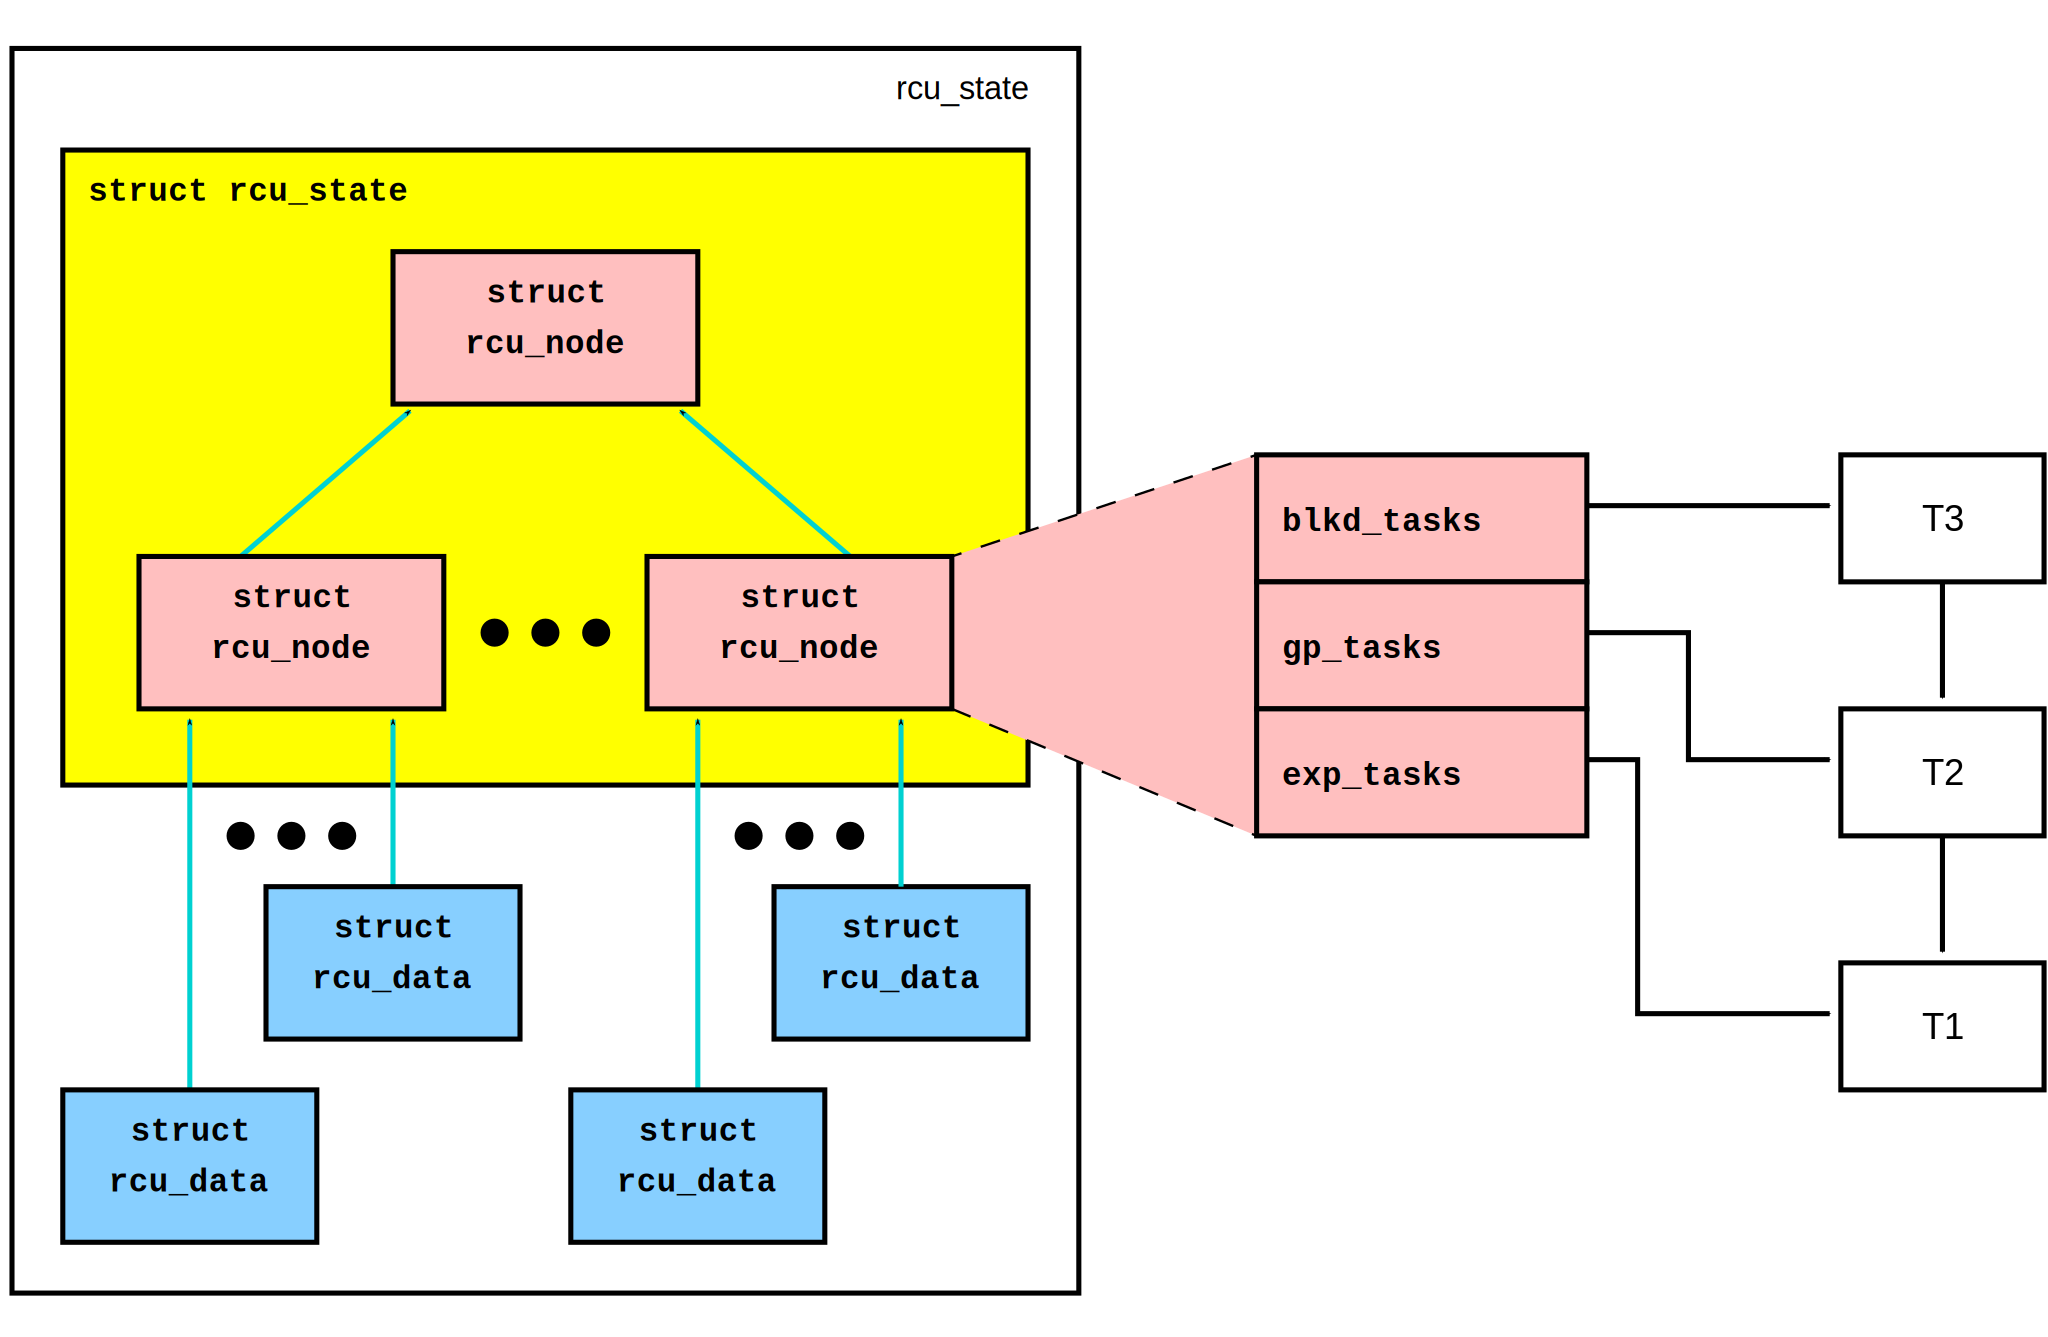
\includegraphics{rcu/design/blkd_task}}
\end{center}

Task~T1 is blocking both grace periods, task~T2 is blocking only the
normal grace period, and task~T3 is blocking neither grace period.
Note
that these tasks will not remove themselves from this list immediately
upon resuming execution.
They will instead remain on the list until they
execute the outermost \co{rcu_read_unlock()} that ends their RCU
read-side critical section.

The \co{->wait_blkd_tasks} field indicates whether or not the current
grace period is waiting on a blocked task.

\paragraph{Sizing the \texttt{rcu\_node} Array}

The \co{rcu_node} array is sized via a series of C-preprocessor
expressions as follows:

\begin{fcvlabel}[ln:rcu:design:data1]
\begin{VerbatimN}[breaklines=true,xleftmargin=1pt,xrightmargin=0pt,commandchars=\%\@\$]
	#ifdef CONFIG_RCU_FANOUT
	#define RCU_FANOUT CONFIG_RCU_FANOUT
	#else
	# ifdef CONFIG_64BIT
	# define RCU_FANOUT 64
	# else
	# define RCU_FANOUT 32
	# endif
	#endif

	#ifdef CONFIG_RCU_FANOUT_LEAF     %lnlbl@confleaf:if$
	#define RCU_FANOUT_LEAF CONFIG_RCU_FANOUT_LEAF
	#else
	# ifdef CONFIG_64BIT
	# define RCU_FANOUT_LEAF 64
	# else
	# define RCU_FANOUT_LEAF 32
	# endif
	#endif                            %lnlbl@confleaf:endif$

	#define RCU_FANOUT_1        (RCU_FANOUT_LEAF) %lnlbl@fanout1$
	#define RCU_FANOUT_2        (RCU_FANOUT_1 * RCU_FANOUT)
	#define RCU_FANOUT_3        (RCU_FANOUT_2 * RCU_FANOUT)
	#define RCU_FANOUT_4        (RCU_FANOUT_3 * RCU_FANOUT) %lnlbl@fanout4$

	#if NR_CPUS <= RCU_FANOUT_1       %lnlbl@cpus:if$
	#  define RCU_NUM_LVLS        1         %lnlbl@lvls1$
	#  define NUM_RCU_LVL_0        1        %lnlbl@lvl01$
	#  define NUM_RCU_NODES        NUM_RCU_LVL_0
	#  define NUM_RCU_LVL_INIT    { NUM_RCU_LVL_0 }
	#  define RCU_NODE_NAME_INIT  { "rcu_node_0" }  %lnlbl@nodenameinit1$
	#  define RCU_FQS_NAME_INIT   { "rcu_node_fqs_0" }
	#  define RCU_EXP_NAME_INIT   { "rcu_node_exp_0" }  %lnlbl@expnameinit1$
	#elif NR_CPUS <= RCU_FANOUT_2
	#  define RCU_NUM_LVLS        2         %lnlbl@lvls2$
	#  define NUM_RCU_LVL_0        1        %lnlbl@lvl02$
	#  define NUM_RCU_LVL_1        DIV_ROUND_UP(NR_CPUS, RCU_FANOUT_1) %lnlbl@lvl12$
	#  define NUM_RCU_NODES        (NUM_RCU_LVL_0 + NUM_RCU_LVL_1)
	#  define NUM_RCU_LVL_INIT    { NUM_RCU_LVL_0, NUM_RCU_LVL_1 }
	#  define RCU_NODE_NAME_INIT  { "rcu_node_0", "rcu_node_1" } %lnlbl@nodenameinit2$
	#  define RCU_FQS_NAME_INIT   { "rcu_node_fqs_0", "rcu_node_fqs_1" }
	#  define RCU_EXP_NAME_INIT   { "rcu_node_exp_0", "rcu_node_exp_1" } %lnlbl@expnameinit2$
	#elif NR_CPUS <= RCU_FANOUT_3
	#  define RCU_NUM_LVLS        3         %lnlbl@lvls3$
	#  define NUM_RCU_LVL_0        1        %lnlbl@lvl03$
	#  define NUM_RCU_LVL_1        DIV_ROUND_UP(NR_CPUS, RCU_FANOUT_2) %lnlbl@lvl13$
	#  define NUM_RCU_LVL_2        DIV_ROUND_UP(NR_CPUS, RCU_FANOUT_1) %lnlbl@lvl23$
	#  define NUM_RCU_NODES        (NUM_RCU_LVL_0 + NUM_RCU_LVL_1 + NUM_RCU_LVL_2)
	#  define NUM_RCU_LVL_INIT    { NUM_RCU_LVL_0, NUM_RCU_LVL_1, NUM_RCU_LVL_2 }
	#  define RCU_NODE_NAME_INIT  { "rcu_node_0", "rcu_node_1", "rcu_node_2" } %lnlbl@nodenameinit3$
	#  define RCU_FQS_NAME_INIT   { "rcu_node_fqs_0", "rcu_node_fqs_1", "rcu_node_fqs_2" }
	#  define RCU_EXP_NAME_INIT   { "rcu_node_exp_0", "rcu_node_exp_1", "rcu_node_exp_2" } %lnlbl@expnameinit3$
	#elif NR_CPUS <= RCU_FANOUT_4
	#  define RCU_NUM_LVLS        4         %lnlbl@lvls4$
	#  define NUM_RCU_LVL_0        1        %lnlbl@lvl04$
	#  define NUM_RCU_LVL_1        DIV_ROUND_UP(NR_CPUS, RCU_FANOUT_3) %lnlbl@lvl14$
	#  define NUM_RCU_LVL_2        DIV_ROUND_UP(NR_CPUS, RCU_FANOUT_2)
	#  define NUM_RCU_LVL_3        DIV_ROUND_UP(NR_CPUS, RCU_FANOUT_1) %lnlbl@lvl34$
	#  define NUM_RCU_NODES        (NUM_RCU_LVL_0 + NUM_RCU_LVL_1 + NUM_RCU_LVL_2 + NUM_RCU_LVL_3)
	#  define NUM_RCU_LVL_INIT    { NUM_RCU_LVL_0, NUM_RCU_LVL_1, NUM_RCU_LVL_2, NUM_RCU_LVL_3 }
	#  define RCU_NODE_NAME_INIT  { "rcu_node_0", "rcu_node_1", "rcu_node_2", "rcu_node_3" } %lnlbl@nodenameinit4$
	#  define RCU_FQS_NAME_INIT   { "rcu_node_fqs_0", "rcu_node_fqs_1", "rcu_node_fqs_2", "rcu_node_fqs_3" }
	#  define RCU_EXP_NAME_INIT   { "rcu_node_exp_0", "rcu_node_exp_1", "rcu_node_exp_2", "rcu_node_exp_3" }  %lnlbl@expnameinit4$
	#else         %lnlbl@cpus:else$
	# error "CONFIG_RCU_FANOUT insufficient for NR_CPUS"
	#endif        %lnlbl@cpus:endif$
\end{VerbatimN}
\end{fcvlabel}

\begin{fcvref}[ln:rcu:design:data1]
The maximum number of levels in the \co{rcu_node} structure is currently
limited to four, as specified by \clnrefrange{fanout1}{fanout4} % lines 21--24
and the structure of the
subsequent \qco{if} statement.
For 32-bit systems, this allows
\co{16*32*32*32=524,288} CPUs, which should be sufficient for the next few
years at least.
For 64-bit systems, \co{16*64*64*64=4,194,304} CPUs is
allowed, which should see us through the next decade or so.
This
four-level tree also allows kernels built with \co{CONFIG_RCU_FANOUT=8}
to support up to 4096 CPUs, which might be useful in very large systems
having eight CPUs per socket (but please note that no one has yet shown
any measurable performance degradation due to misaligned socket and
\co{rcu_node} boundaries).
In addition, building kernels with a full four
levels of \co{rcu_node} tree permits better testing of RCU's
combining-tree code.

The \co{RCU_FANOUT} symbol controls how many children are permitted at
each non-leaf level of the \co{rcu_node} tree.
If the
\co{CONFIG_RCU_FANOUT} Kconfig option is not specified, it is set based
on the word size of the system, which is also the Kconfig default.

The \co{RCU_FANOUT_LEAF} symbol controls how many CPUs are handled by
each leaf \co{rcu_node} structure.
Experience has shown that allowing a
given leaf \co{rcu_node} structure to handle 64 CPUs, as permitted by the
number of bits in the \co{->qsmask} field on a 64-bit system, results in
excessive contention for the leaf \co{rcu_node} structures' \co{->lock}
fields.
The number of CPUs per leaf \co{rcu_node} structure is therefore
limited to 16 given the default value of \co{CONFIG_RCU_FANOUT_LEAF}.
If
\co{CONFIG_RCU_FANOUT_LEAF} is unspecified, the value selected is based
on the word size of the system, just as for \co{CONFIG_RCU_FANOUT}.
\Clnrefrange{confleaf:if}{confleaf:endif} % Lines 11--19
perform this computation.

\Clnrefrange{fanout1}{fanout4} % Lines 21--24
compute the maximum number of CPUs supported by a
single-level (which contains a single \co{rcu_node} structure),
two-level, three-level, and four-level \co{rcu_node} tree, respectively,
given the fanout specified by \co{RCU_FANOUT} and \co{RCU_FANOUT_LEAF}.
These numbers of CPUs are retained in the \co{RCU_FANOUT_1},
\co{RCU_FANOUT_2}, \co{RCU_FANOUT_3}, and \co{RCU_FANOUT_4} C-preprocessor
variables, respectively.

These variables are used to control the C-preprocessor \co{#if} statement
spanning \clnrefrange{cpus:if}{cpus:endif} % lines 26--66
that computes the number of \co{rcu_node} structures
required for each level of the tree, as well as the number of levels
required.
The number of levels is placed in the \co{NUM_RCU_LVLS}
C-preprocessor variable by \clnref{lvls1,lvls2,lvls3,lvls4}. % lines 27, 35, 44, and 54.
The number of
\co{rcu_node} structures for the topmost level of the tree is always
exactly one, and this value is unconditionally placed into
\co{NUM_RCU_LVL_0} by \clnref{lvl01,lvl02,lvl03,lvl04}. % lines 28, 36, 45, and 55.
The rest of the levels
(if any) of the \co{rcu_node} tree are computed by dividing the maximum
number of CPUs by the fanout supported by the number of levels from the
current level down, rounding up.
This computation is performed by
lines~\lnref{lvl12}, \lnref{lvl13}--\lnref{lvl23}, and~\lnref{lvl14}--\lnref{lvl34}. % 37, 46--47, and~56--58.
Lines~\lnref{nodenameinit1}--\lnref{expnameinit1}, % 31--33
\lnref{nodenameinit2}--\lnref{expnameinit2}, % 40--42
\lnref{nodenameinit3}--\lnref{expnameinit3}, % 50--52
and~\lnref{nodenameinit4}--\lnref{expnameinit4} % and~62--63
create
initializers for lockdep lock-class names.
Finally, \clnrefrange{cpus:else}{cpus:endif} % lines 64--66
produce
an error if the maximum number of CPUs is too large for the specified
fanout.
\end{fcvref}

\subsubsection{The \texttt{rcu\_segcblist} Structure}

The \co{rcu_segcblist} structure maintains a segmented list of callbacks
as follows:

\begin{VerbatimN}
	#define RCU_DONE_TAIL        0
	#define RCU_WAIT_TAIL        1
	#define RCU_NEXT_READY_TAIL  2
	#define RCU_NEXT_TAIL        3
	#define RCU_CBLIST_NSEGS     4

	struct rcu_segcblist {
		struct rcu_head *head;
		struct rcu_head **tails[RCU_CBLIST_NSEGS];
		unsigned long gp_seq[RCU_CBLIST_NSEGS];
		long len;
		long len_lazy;
	};
\end{VerbatimN}

The segments are as follows:

\begin{description}
\item[\tco{RCU_DONE_TAIL}:]
   Callbacks whose grace periods have elapsed.
   These
   callbacks are ready to be invoked.
\item[\tco{RCU_WAIT_TAIL}:]
   Callbacks that are waiting for the current grace
   period.
   Note that different CPUs can have different ideas about which
   grace period is current, hence the \co{->gp_seq} field.
\item[\tco{RCU_NEXT_READY_TAIL}:]
   Callbacks waiting for the next grace period
   to start.
\item[\tco{RCU_NEXT_TAIL}:]
   Callbacks that have not yet been associated with a
   grace period.
\end{description}

The \co{->head} pointer references the first callback or is \co{NULL} if
the list contains no callbacks (which is \emph{not} the same as being empty).
Each element of the \co{->tails[]} array references the \co{->next}
pointer of the last callback in the corresponding segment of the list,
or the list's \co{->head} pointer if that segment and all previous
segments are empty.
If the corresponding segment is empty but some
previous segment is not empty, then the array element is identical to
its predecessor.
Older callbacks are closer to the head of the list, and
new callbacks are added at the tail.
This relationship between the
\co{->head} pointer, the \co{->tails[]} array, and the callbacks is shown
in this diagram:

\begin{center}
\resizebox{.7\columnwidth}{!}{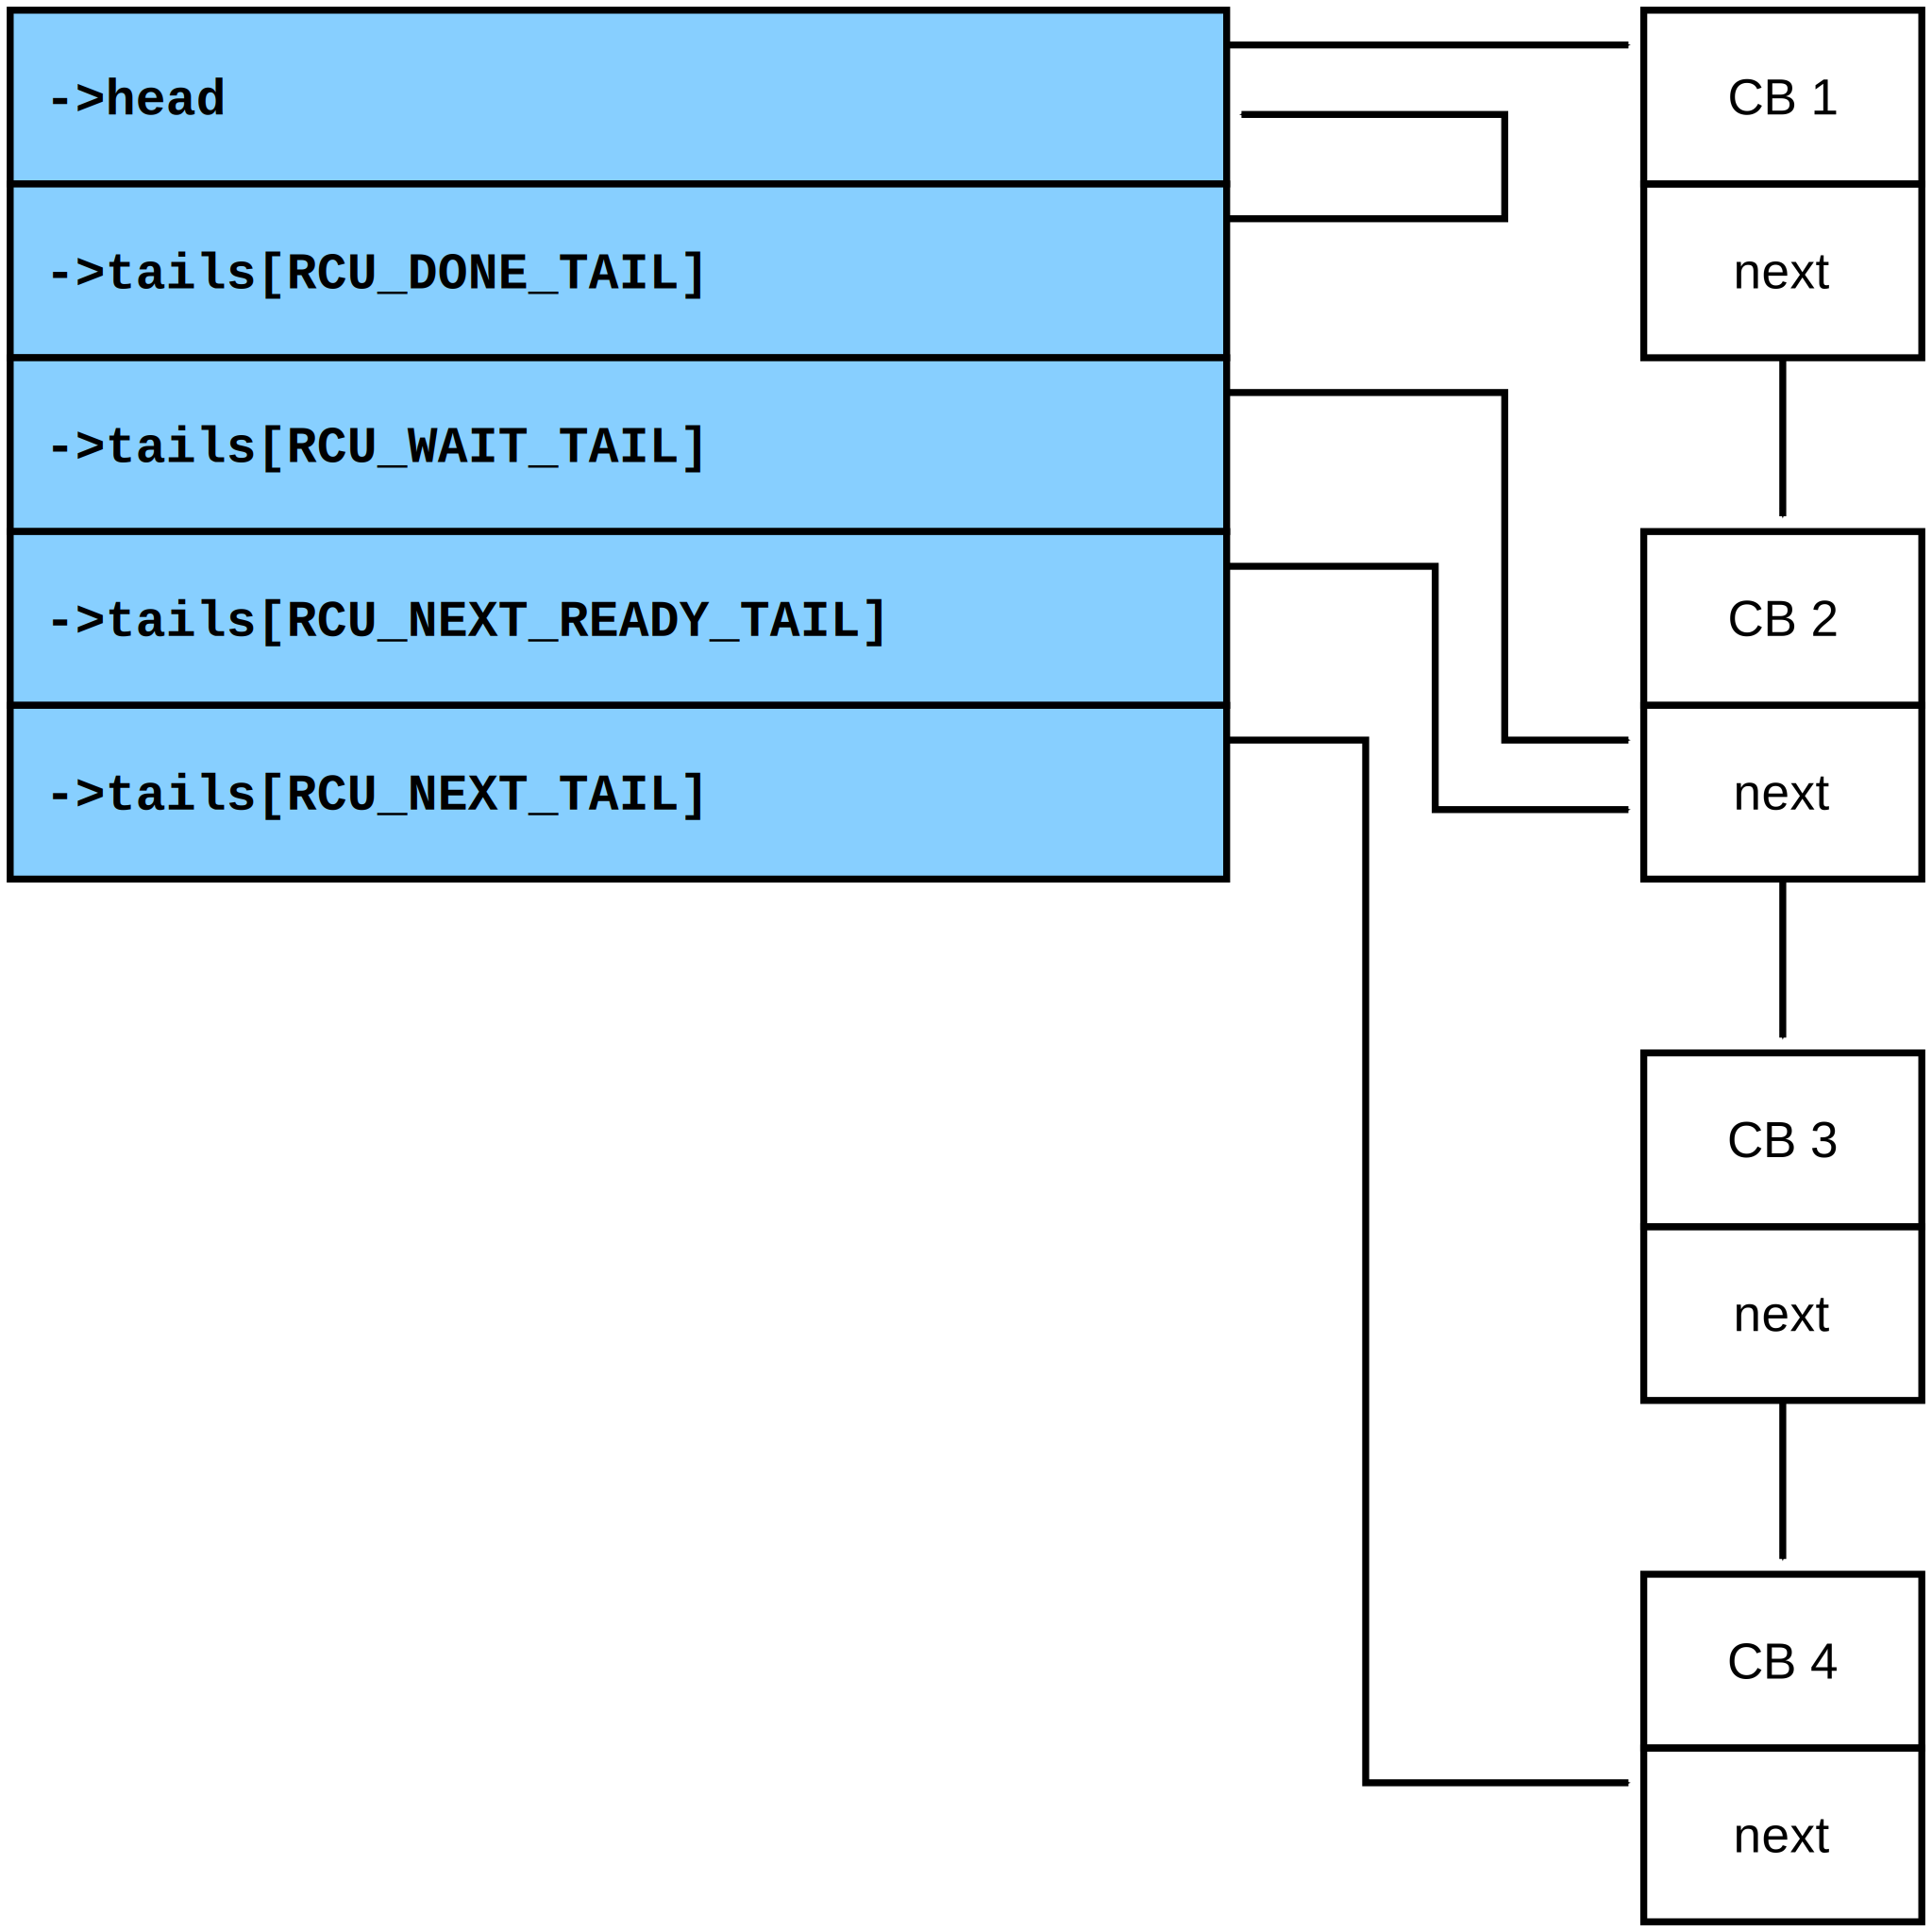
\includegraphics{rcu/design/nxtlist}}
\end{center}

In this figure, the \co{->head} pointer references the first RCU callback
in the list.
The \co{->tails[RCU_DONE_TAIL]} array element references the
\co{->head} pointer itself, indicating that none of the callbacks is
ready to invoke.
The \co{->tails[RCU_WAIT_TAIL]} array element references
callback CB~2's \co{->next} pointer, which indicates that CB~1 and CB~2
are both waiting on the current grace period, give or take possible
disagreements about exactly which grace period is the current one.
The
\co{->tails[RCU_NEXT_READY_TAIL]} array element references the same RCU
callback that \co{->tails[RCU_WAIT_TAIL]} does, which indicates that
there are no callbacks waiting on the next RCU grace period.
The
\co{->tails[RCU_NEXT_TAIL]} array element references CB~4's \co{->next}
pointer, indicating that all the remaining RCU callbacks have not yet
been assigned to an RCU grace period.
Note that the
\co{->tails[RCU_NEXT_TAIL]} array element always references the last RCU
callback's \co{->next} pointer unless the callback list is empty, in
which case it references the \co{->head} pointer.

There is one additional important special case for the
\co{->tails[RCU_NEXT_TAIL]} array element:
It can be \co{NULL} when this
list is \emph{disabled}.
Lists are disabled when the corresponding CPU is
offline or when the corresponding CPU's callbacks are offloaded to a
kthread, both of which are described elsewhere.

CPUs advance their callbacks from the \co{RCU_NEXT_TAIL} to the
\co{RCU_NEXT_READY_TAIL} to the \co{RCU_WAIT_TAIL} to the
\co{RCU_DONE_TAIL} list segments as grace periods advance.

The \co{->gp_seq[]} array records grace-period numbers corresponding to
the list segments.
This is what allows different CPUs to have different
ideas as to which is the current grace period while still avoiding
premature invocation of their callbacks.
In particular, this allows CPUs
that go idle for extended periods to determine which of their callbacks
are ready to be invoked after reawakening.

The \co{->len} counter contains the number of callbacks in \co{->head},
and the \co{->len_lazy} contains the number of those callbacks that are
known to only free memory, and whose invocation can therefore be safely
deferred.

\begin{Note}
   Important:

   It is the \co{->len} field that determines whether or
   not there are callbacks associated with this \co{rcu_segcblist}
   structure, \emph{not} the \co{->head} pointer.
   The reason for this is that all
   the ready-to-invoke callbacks (that is, those in the \co{RCU_DONE_TAIL}
   segment) are extracted all at once at callback-invocation time
   (\co{rcu_do_batch}), due to which \co{->head} may be set to \co{NULL} if there
   are no not-done callbacks remaining in the \co{rcu_segcblist}.
   If
   callback invocation must be postponed, for example, because a
   high-priority process just woke up on this CPU, then the remaining
   callbacks are placed back on the \co{RCU_DONE_TAIL} segment and
   \co{->head} once again points to the start of the segment.
   In short, the
   head field can briefly be \co{NULL} even though the CPU has callbacks
   present the entire time.
   Therefore, it is not appropriate to test the
   \co{->head} pointer for \co{NULL}.
\end{Note}

In contrast, the \co{->len} and \co{->len_lazy} counts are adjusted only
after the corresponding callbacks have been invoked.
This means that the
\co{->len} count is zero only if the \co{rcu_segcblist} structure really
is devoid of callbacks.
Of course, off-CPU sampling of the \co{->len}
count requires careful use of appropriate synchronization, for example,
memory barriers.
This synchronization can be a bit subtle, particularly
in the case of \co{rcu_barrier()}.

\subsubsection{The \texttt{rcu\_data} Structure}

The \co{rcu_data} maintains the per-CPU state for the RCU subsystem.
The
fields in this structure may be accessed only from the corresponding CPU
(and from tracing) unless otherwise stated.
This structure is the focus
of quiescent-state detection and RCU callback queuing.
It also tracks
its relationship to the corresponding leaf \co{rcu_node} structure to
allow more-efficient propagation of quiescent states up the \co{rcu_node}
combining tree.
Like the \co{rcu_node} structure, it provides a local
copy of the grace-period information to allow for-free synchronized
access to this information from the corresponding CPU\@.
Finally, this
structure records past dyntick-idle state for the corresponding CPU and
also tracks statistics.

The \co{rcu_data} structure's fields are discussed, singly and in groups,
in the following sections.

\paragraph{Connection to Other Data Structures}

This portion of the \co{rcu_data} structure is declared as follows:

\begin{VerbatimN}
		int cpu;
		struct rcu_node *mynode;
		unsigned long grpmask;
		bool beenonline;
\end{VerbatimN}

The \co{->cpu} field contains the number of the corresponding CPU and the
\co{->mynode} field references the corresponding \co{rcu_node} structure.
The \co{->mynode} is used to propagate quiescent states up the combining
tree.
These two fields are constant and therefore do not require
synchronization.

The \co{->grpmask} field indicates the bit in the \co{->mynode->qsmask}
corresponding to this \co{rcu_data} structure, and is also used when
propagating quiescent states.
The \co{->beenonline} flag is set whenever
the corresponding CPU comes online, which means that the debugfs tracing
need not dump out any \co{rcu_data} structure for which this flag is not
set.

\paragraph{Quiescent-State and Grace-Period Tracking}

This portion of the \co{rcu_data} structure is declared as follows:

\begin{VerbatimN}
		unsigned long gp_seq;
		unsigned long gp_seq_needed;
		bool cpu_no_qs;
		bool core_needs_qs;
		bool gpwrap;
\end{VerbatimN}

The \co{->gp_seq} field is the counterpart of the field of the same name
in the \co{rcu_state} and \co{rcu_node} structures.
The
\co{->gp_seq_needed} field is the counterpart of the field of the same
name in the \co{rcu_node} structure.
They may each lag up to one behind their
\co{rcu_node} counterparts, but in \co{CONFIG_NO_HZ_IDLE} and
\co{CONFIG_NO_HZ_FULL} kernels can lag arbitrarily far behind for CPUs in
dyntick-idle mode (but these counters will catch up upon exit from
dyntick-idle mode).
If the lower two bits of a given \co{rcu_data}
structure's \co{->gp_seq} are zero, then this \co{rcu_data} structure
believes that RCU is idle.

\QuickQuiz{
  All this replication of the grace period numbers can only cause
  massive confusion.
  Why not just keep a global sequence number and be
  done with it???
}\QuickQuizAnswer{
  Because if there was only a single global sequence numbers, there
  would need to be a single global lock to allow safely accessing and
  updating it.
  And if we are not going to have a single global lock, we
  need to carefully manage the numbers on a per-node basis.
  Recall from
  the answer to a previous Quick Quiz that the consequences of applying
  a previously sampled quiescent state to the wrong grace period are
  quite severe.
}\QuickQuizEnd

The \co{->cpu_no_qs} flag indicates that the CPU has not yet passed
through a quiescent state, while the \co{->core_needs_qs} flag indicates
that the RCU core needs a quiescent state from the corresponding CPU\@.
The \co{->gpwrap} field indicates that the corresponding CPU has remained
idle for so long that the \co{gp_seq} counter is in danger of overflow,
which will cause the CPU to disregard the values of its counters on its
next exit from idle.

\paragraph{RCU Callback Handling}

In the absence of CPU-hotplug events, RCU callbacks are invoked by the
same CPU that registered them.
This is strictly a cache-locality
optimization: callbacks can and do get invoked on CPUs other than the
one that registered them.
After all, if the CPU that registered a given
callback has gone offline before the callback can be invoked, there
really is no other choice.

This portion of the \co{rcu_data} structure is declared as follows:

\begin{VerbatimN}
	struct rcu_segcblist cblist;
	long qlen_last_fqs_check;
	unsigned long n_cbs_invoked;
	unsigned long n_nocbs_invoked;
	unsigned long n_cbs_orphaned;
	unsigned long n_cbs_adopted;
	unsigned long n_force_qs_snap;
	long blimit;
\end{VerbatimN}

The \co{->cblist} structure is the segmented callback list described
earlier.
The CPU advances the callbacks in its \co{rcu_data} structure
whenever it notices that another RCU grace period has completed.
The CPU
detects the completion of an RCU grace period by noticing that the value
of its \co{rcu_data} structure's \co{->gp_seq} field differs from that of
its leaf \co{rcu_node} structure.
Recall that each \co{rcu_node}
structure's \co{->gp_seq} field is updated at the beginnings and ends of
each grace period.

The \co{->qlen_last_fqs_check} and \co{->n_force_qs_snap} coordinate the
forcing of quiescent states from \co{call_rcu()} and friends when
callback lists grow excessively long.

The \co{->n_cbs_invoked}, \co{->n_cbs_orphaned}, and \co{->n_cbs_adopted}
fields count the number of callbacks invoked, sent to other CPUs when
this CPU goes offline, and received from other CPUs when those other
CPUs go offline.
The \co{->n_nocbs_invoked} is used when the CPU's
callbacks are offloaded to a kthread.

Finally, the \co{->blimit} counter is the maximum number of RCU callbacks
that may be invoked at a given time.

\paragraph{Dyntick-Idle Handling}

This portion of the \co{rcu_data} structure is declared as follows:

\begin{VerbatimN}
		int watching_snap;
		unsigned long dynticks_fqs;
\end{VerbatimN}

The \co{->watching_snap} field is used to take a snapshot of the
corresponding CPU's dyntick-idle state when forcing quiescent states,
and is therefore accessed from other CPUs.
Finally, the
\co{->dynticks_fqs} field is used to count the number of times this CPU
is determined to be in dyntick-idle state, and is used for tracing and
debugging purposes.

This portion of the \co{rcu_data} structure is declared as follows:

\begin{VerbatimN}
		long nesting;
		long nmi_nesting;
		atomic_t dynticks;
		bool rcu_need_heavy_qs;
		bool rcu_urgent_qs;
\end{VerbatimN}

These fields in the \co{rcu_data} structure maintain the per-CPU dyntick-idle
state for the corresponding CPU\@.
The fields may be accessed only from
the corresponding CPU (and from tracing) unless otherwise stated.

The \co{->nesting} field counts the nesting depth of process
execution, so that in normal circumstances this counter has value zero
or one.
NMIs, irqs, and tracers are counted by the
\co{->nmi_nesting} field.
Because NMIs cannot be masked, changes
to this variable have to be undertaken carefully using an algorithm
provided by Andy Lutomirski.
The initial transition from idle adds one,
and nested transitions add two, so that a nesting level of five is
represented by a \co{->nmi_nesting} value of nine.
This counter
can therefore be thought of as counting the number of reasons why this
CPU cannot be permitted to enter dyntick-idle mode, aside from
process-level transitions.

However, it turns out that when running in non-idle kernel context, the
Linux kernel is fully capable of entering interrupt handlers that never
exit and perhaps also vice versa.
Therefore, whenever the
\co{->nesting} field is incremented up from zero, the
\co{->nmi_nesting} field is set to a large positive number, and
whenever the \co{->nesting} field is decremented down to zero,
the \co{->nmi_nesting} field is set to zero.
Assuming that
the number of misnested interrupts is not sufficient to overflow the
counter, this approach corrects the \co{->nmi_nesting} field
every time the corresponding CPU enters the idle loop from process
context.

The \co{->dynticks} field counts the corresponding CPU's transitions to
and from either dyntick-idle or user mode, so that this counter has an
even value when the CPU is in dyntick-idle mode or user mode and an odd
value otherwise.
The transitions to/from user mode need to be counted
for user mode adaptive-ticks support (see \path{Documentation/timers/no_hz.rst}).

The \co{->rcu_need_heavy_qs} field is used to record the fact that the
RCU core code would really like to see a quiescent state from the
corresponding CPU, so much so that it is willing to call for
heavy-weight dyntick-counter operations.
This flag is checked by RCU's
context-switch and \co{cond_resched()} code, which provide a momentary
idle sojourn in response.

Finally, the \co{->rcu_urgent_qs} field is used to record the fact that
the RCU core code would really like to see a quiescent state from the
corresponding CPU, with the various other fields indicating just how
badly RCU wants this quiescent state.
This flag is checked by RCU's
context-switch path (\co{rcu_note_context_switch}) and the \co{cond_resched}
code.

\QuickQuiz{
  Why not simply combine the \co{->nesting} and
  \co{->nmi_nesting} counters into a single counter that just
  counts the number of reasons that the corresponding CPU is non-idle?
}\QuickQuizAnswer{
  Because this would fail in the presence of interrupts whose handlers
  never return and of handlers that manage to return from a made-up
  interrupt.
}\QuickQuizEnd

Additional fields are present for some special-purpose builds, and are
discussed separately.

\subsubsection{The \texttt{rcu\_head} Structure}

Each \co{rcu_head} structure represents an RCU callback.
These structures
are normally embedded within RCU-protected data structures whose
algorithms use asynchronous grace periods.
In contrast, when using
algorithms that block waiting for RCU grace periods, RCU users need not
provide \co{rcu_head} structures.

The \co{rcu_head} structure has fields as follows:

\begin{VerbatimN}
		struct rcu_head *next;
		void (*func)(struct rcu_head *head);
\end{VerbatimN}

The \co{->next} field is used to link the \co{rcu_head} structures
together in the lists within the \co{rcu_data} structures.
The \co{->func}
field is a pointer to the function to be called when the callback is
ready to be invoked, and this function is passed a pointer to the
\co{rcu_head} structure.
However, \co{kfree_rcu()} uses the \co{->func}
field to record the offset of the \co{rcu_head} structure within the
enclosing RCU-protected data structure.

Both of these fields are used internally by RCU\@.
From the viewpoint of
RCU users, this structure is an opaque ``cookie''.

\QuickQuiz{
  Given that the callback function \co{->func} is passed a pointer to
  the \co{rcu_head} structure, how is that function supposed to find the
  beginning of the enclosing RCU-protected data structure?
}\QuickQuizAnswer{
  In actual practice, there is a separate callback function per type of
  RCU-protected data structure.
  The callback function can therefore use
  the \co{container_of()} macro in the Linux kernel (or other
  pointer-manipulation facilities in other software environments) to
  find the beginning of the enclosing structure.
}\QuickQuizEnd

\subsubsection{RCU-Specific Fields in the \texttt{task\_struct} Structure}

The \co{CONFIG_PREEMPT_RCU} implementation uses some additional fields in
the \co{task_struct} structure:

\begin{VerbatimN}
	#ifdef CONFIG_PREEMPT_RCU
		int rcu_read_lock_nesting;
		union rcu_special rcu_read_unlock_special;
		struct list_head rcu_node_entry;
		struct rcu_node *rcu_blocked_node;
	#endif /* #ifdef CONFIG_PREEMPT_RCU */
	#ifdef CONFIG_TASKS_RCU
		unsigned long rcu_tasks_nvcsw;
		bool rcu_tasks_holdout;
		struct list_head rcu_tasks_holdout_list;
		int rcu_tasks_idle_cpu;
	#endif /* #ifdef CONFIG_TASKS_RCU */
\end{VerbatimN}

The \co{->rcu_read_lock_nesting} field records the nesting level for RCU
read-side critical sections, and the \co{->rcu_read_unlock_special} field
is a bitmask that records special conditions that require
\co{rcu_read_unlock()} to do additional work.
The \co{->rcu_node_entry}
field is used to form lists of tasks that have blocked within
preemptible-RCU read-side critical sections and the
\co{->rcu_blocked_node} field references the \co{rcu_node} structure whose
list this task is a member of, or \co{NULL} if it is not blocked within a
preemptible-RCU read-side critical section.

The \co{->rcu_tasks_nvcsw} field tracks the number of voluntary context
switches that this task had undergone at the beginning of the current
tasks-RCU grace period, \co{->rcu_tasks_holdout} is set if the current
tasks-RCU grace period is waiting on this task,
\co{->rcu_tasks_holdout_list} is a list element enqueuing this task on
the holdout list, and \co{->rcu_tasks_idle_cpu} tracks which CPU this
idle task is running, but only if the task is currently running, that
is, if the CPU is currently idle.

\subsubsection{Accessor Functions}

The following listing shows the \co{rcu_get_root()},
\co{rcu_for_each_node_breadth_first} and \co{rcu_for_each_leaf_node()}
function and macros:

\begin{VerbatimN}
	static struct rcu_node *rcu_get_root(struct rcu_state *rsp)
	{
		return &rsp->node[0];
	}

	#define rcu_for_each_node_breadth_first(rsp, rnp) \
	        for ((rnp) = &(rsp)->node[0]; \
	             (rnp) < &(rsp)->node[NUM_RCU_NODES]; (rnp)++)

	#define rcu_for_each_leaf_node(rsp, rnp) \
	        for ((rnp) = (rsp)->level[NUM_RCU_LVLS - 1]; \
	             (rnp) < &(rsp)->node[NUM_RCU_NODES]; (rnp)++)
\end{VerbatimN}

The \co{rcu_get_root()} simply returns a pointer to the first element of
the specified \co{rcu_state} structure's \co{->node[]} array, which is the
root \co{rcu_node} structure.

As noted earlier, the \co{rcu_for_each_node_breadth_first()} macro takes
advantage of the layout of the \co{rcu_node} structures in the
\co{rcu_state} structure's \co{->node[]} array, performing a breadth-first
traversal by simply traversing the array in order.
Similarly, the
\co{rcu_for_each_leaf_node()} macro traverses only the last part of the
array, thus traversing only the leaf \co{rcu_node} structures.

\QuickQuiz{
  What does \co{rcu_for_each_leaf_node()} do if the \co{rcu_node} tree
  contains only a single node?
}\QuickQuizAnswer{
  In the single-node case, \co{rcu_for_each_leaf_node()} traverses the
  single node.
}\QuickQuizEnd

\subsection{Summary}

So the state of RCU is represented by an \co{rcu_state} structure, which
contains a combining tree of \co{rcu_node} and \co{rcu_data} structures.
Finally, in \co{CONFIG_NO_HZ_IDLE} kernels, each CPU's dyntick-idle state
is tracked by dynticks-related fields in the \co{rcu_data} structure.
If
you made it this far, you are well prepared to read the code
walkthroughs in the other articles in this series.

\subsection{Acknowledgments}

I owe thanks to Cyrill Gorcunov, Mathieu Desnoyers, Dhaval Giani, Paul
Turner, Abhishek Srivastava, Matt Kowalczyk, and Serge Hallyn for
helping me get this document into a more human-readable state.

\subsection{Legal Statement}

This work represents the view of the author and does not necessarily
represent the view of IBM\@.

Linux is a registered trademark of Linus Torvalds.

Other company, product, and service names may be trademarks or service
marks of others.



\QuickQuizAnswers

\end{document}
